\documentclass[12pt, a4paper]{book}

% -------------------------------------------------------------------
% Packages
% -------------------------------------------------------------------
\usepackage[utf8]{inputenc}
\usepackage[T1]{fontenc}
\usepackage{lmodern}       % Improved font rendering
\usepackage{geometry}      % Page margins
\usepackage{amsmath}       % Math formatting
\usepackage{amssymb}       % Math symbols
\usepackage{graphicx}      % Handling images
\usepackage{float}         % Force figure placement with [H]
\usepackage{fancyhdr}      % Custom headers/footers
\usepackage{enumitem}      % Custom lists
\usepackage{hyperref}      % Hyperlinks for navigation
\usepackage{caption}       % Better caption formatting
\usepackage{tikz}
\usepackage{cancel}
\usepackage{array}
\usepackage{ragged2e}
\usepackage[titletoc]{appendix}
\usepackage{booktabs}
\usepackage[table,xcdraw]{xcolor}
\usepackage{mathtools}
\usetikzlibrary{shapes, arrows.meta, positioning, calc, fit, backgrounds}
\usetikzlibrary{positioning,arrows}
\usepackage[american]{circuitikz}
\usetikzlibrary{shapes.symbols}
\usetikzlibrary{patterns}
\usetikzlibrary{shapes.geometric}
\usetikzlibrary{fit}
\usepackage[scaled]{helvet}               % Load Helvetica font
\renewcommand{\familydefault}{\sfdefault} % Set it as the default text font
\usepackage{sfmath}                       % Make math equations Sans-Serif too
\usepackage{algorithm}
\usepackage{algpseudocode}
\usepackage[numbers,sort&compress]{natbib}  % Bibliography support
% -------------------------------------------------------------------

\usepackage{tabularx} % For adjustable table widths
% Table of Contents: widen number columns to prevent overlap (e.g., 10.15)
\makeatletter
\renewcommand{\l@section}{\@dottedtocline{1}{1.5em}{3.0em}}
\renewcommand{\l@subsection}{\@dottedtocline{2}{4.5em}{3.8em}}
\renewcommand{\l@subsubsection}{\@dottedtocline{3}{8.3em}{4.5em}}
\makeatother

% Page Setup
% -------------------------------------------------------------------
\geometry{top=2cm, bottom=2cm, left=2cm, right=2cm}
\setlength{\parskip}{1em}
\setlength{\parindent}{0pt}
\usepackage{pgfplots}
\pgfplotsset{compat=1.18} % Or 'compat=newest' to ensure future compatibility

% Header and Footer configuration
% Header and Footer configuration
\pagestyle{fancy}
\fancyhf{}
\setlength{\headheight}{15pt} % Fixes a common warning
\lhead{\textbf{Model Predictive Control}}
\rhead{\leftmark} % <--- This automatically puts the current Chapter name here
\cfoot{\thepage}
\renewcommand{\chaptermark}[1]{\markboth{Chapter \thechapter: #1}{}}

% ===================================================================
% FANCY EXAMPLE ENVIRONMENT SETUP
% ===================================================================
\usepackage[most]{tcolorbox}
\tcbuselibrary{skins} % <--- Add this line to be 100% sure
% Define a custom color for the examples (A nice Teal)
\definecolor{excolor}{RGB}{0, 128, 128} 
\definecolor{exback}{RGB}{240, 250, 250}

% Define the specific blue color from the image
\definecolor{techblue}{RGB}{0, 160, 230}

% Custom column types for vertical alignment
\newcolumntype{L}[1]{>{\RaggedRight\hspace{0pt}}m{#1}}
\newcolumntype{C}[1]{>{\Centering\hspace{0pt}}m{#1}}

% Define the 'examplebox' environment
\newtcolorbox[auto counter, number within=chapter]{examplebox}[2][]{%
	% General Style
	enhanced, 
	breakable,                    % Allow box to break across pages
	colback=exback,               % Background color
	colframe=excolor,             % Border Color
	coltitle=white,               % Title Font Color
	% Title Box Formatting
	fonttitle=\bfseries\sffamily,
	title={Example~\thetcbcounter: #2}, 
	attach boxed title to top left={xshift=0.5cm, yshift*=-3mm},
	boxed title style={%
		colback=excolor,
		arc=3mm,
		drop lifted shadow=black!30
	},
	% Frame Formatting
	arc=6mm,
	drop fuzzy shadow,            % The shadow behind the main box
	% Margins
	top=5mm,
	bottom=5mm,
	left=5mm,
	right=5mm,
	before upper={\setlength{\parskip}{1em}}, 
	#1 % Allows extra options to be passed
}

% Optional: A 'Solution' separator command to use inside the box
\newcommand{\solution}{\tcbline\textbf{\textsf{Solution:}}\par}

\usepackage{listings}
\usepackage{xcolor}
 \usepackage{tikz-3dplot}
% Define colors for code highlighting
\definecolor{codegreen}{rgb}{0,0.6,0}
\definecolor{codegray}{rgb}{0.5,0.5,0.5}
\definecolor{codepurple}{rgb}{0.58,0,0.82}
\definecolor{backcolour}{rgb}{0.95,0.95,0.92}

% Configure the appearance of code listings
\lstset{
	backgroundcolor=\color{backcolour},   
	commentstyle=\color{codegreen},
	keywordstyle=\color{magenta},
	numberstyle=\tiny\color{codegray},
	stringstyle=\color{codepurple},
	basicstyle=\ttfamily\footnotesize, % Typewriter font
	breakatwhitespace=false,         
	breaklines=true,                 
	captionpos=b,                    
	keepspaces=true,                 
	numbers=left,                    % Line numbers on left
	numbersep=5pt,                  
	showspaces=false,                
	showstringspaces=false,
	showtabs=false,                  
	tabsize=2,
	frame=single,                    % Box around the code
	aboveskip=1.5\baselineskip,      % Space before listing
	belowskip=1.5\baselineskip       % Space after listing
}

\newtheorem{definition}{Definition}
\newtheorem{interpretation}{Interpretation}
\newtheorem{remark}{Remark}
% -------------------------------------------------------------------
% Title Details
% -------------------------------------------------------------------
\title{\textbf{Model Predictive Control}\\ From Foundations to Advanced Topics}

\author{\.Ibrahim K\"u\c c\"ukdemiral }
\date{\today}
% Custom box for Definitions
\newtcolorbox[auto counter, number within=chapter]{defnbox}[1]{
	colback=blue!5!white,
	colframe=blue!75!black,
	fonttitle=\bfseries,
	title={#1},
	before upper={\setlength{\parskip}{1em}} 
}

\newtcolorbox[auto counter, number within=chapter]{alertbox}[1]{
	colback=red!5!white,      % Background color (pale red)
	colframe=red!75!black,    % Frame color (dark red)
	fonttitle=\bfseries,      % Title font style
	title=#1,                  % The title variable
	before upper={\setlength{\parskip}{1em}} 
}

\newtcolorbox[auto counter, number within=chapter]{summarybox}[1]{
	colback=white,           % Background color (change to match your style, e.g., gray!5)
	colframe=black,          % Border color
	colbacktitle=black,      % Title background color
	coltitle=white,          % Title text color
		before upper={\setlength{\parskip}{1em}},
	fonttitle=\bfseries,
	title={#1}             
}
% Add to preamble if needed
\newtcolorbox[auto counter, number within=chapter]{notebox}[1]{
	colback=yellow!5!white, 
	colframe=yellow!75!black, 
	fonttitle=\bfseries, 
	title=#1,
		boxed title style={%
		colback=excolor,
		arc=3mm,
		drop lifted shadow=black!30
	},
		% Frame Formatting
	arc=6mm,
	drop fuzzy shadow,            % The shadow behind the main box
	% Margins
	top=5mm,
	bottom=5mm,
	left=5mm,
	right=5mm,
	before upper={\setlength{\parskip}{1em}}  
	}

\newtcolorbox[auto counter, number within=chapter]{safetybox}[1]{
	colback=red!5!white,
	colframe=red!75!black,
	fonttitle=\bfseries,
	title={#1},
	before upper={\setlength{\parskip}{1em}} 
}

\definecolor{mpcblue}{RGB}{0,115,189}
\definecolor{plantgreen}{RGB}{34,139,34}
\definecolor{obsvorange}{RGB}{217,83,25}
\definecolor{targetpurp}{RGB}{126,47,142}
\definecolor{ctgray}{RGB}{80,80,80}
\definecolor{satred}{RGB}{190,30,45}
\definecolor{sensorgold}{RGB}{180,140,20}
\begin{document}
\raggedbottom
\hypersetup{pageanchor=false}

	\maketitle
	\hypersetup{pageanchor=true}

	% Copyright page (verso of title page)
	\thispagestyle{empty}
	\vspace*{\fill}
	\begin{center}
		\textcopyright{} 2026 \.Ibrahim K\"u\c{c}\"ukdemiral

		\vspace{0.8cm}

		This work is licensed under the Creative Commons Attribution--NonCommercial 4.0\\
		International License (CC BY--NC 4.0).\\[4pt]
		\texttt{\url{https://creativecommons.org/licenses/by-nc/4.0/}}

		\vspace{1.5cm}

		\textbf{How to cite this book}\\[4pt]
		\.Ibrahim K\"u\c{c}\"ukdemiral.\\
		\textit{Model Predictive Control: From Foundations to Advanced Topics.}\\
		2026. \texttt{https://doi.org/10.5281/zenodo.19310682}
	\end{center}
	\vspace*{\fill}
	\cleardoublepage

	% Dedication page
	\thispagestyle{empty}
	\vspace*{\stretch{1}}
	\begin{center}
		\large\itshape
		To Neslihan and Demir
	\end{center}
	\vspace*{\stretch{3}}
	\cleardoublepage

	\tableofcontents
	\newpage
	\chapter*{Foreword}
\addcontentsline{toc}{chapter}{Foreword}

Model Predictive Control (MPC) is an optimisation-based control methodology. By explicitly exploiting a dynamical model of the system, MPC predicts future behaviour and determines control actions by solving a constrained optimisation problem in real time. This distinguishes MPC from classical feedback controllers such as PID or lead--lag compensators, which rely on fixed control laws designed offline.

Initially developed in the process industries~\cite{Qin2003}, MPC has since been adopted in robotics (trajectory tracking under actuator limits), autonomous vehicles (path planning with obstacle avoidance), and aerospace (powered descent guidance under thrust constraints). Its ability to handle multivariable dynamics and hard constraints within a single optimisation framework makes it applicable wherever classical single-loop controllers reach their limits.

\paragraph{Aim and scope.}
This book has been written with a strongly practical emphasis. The primary objective is to introduce MPC in a way that allows readers to apply the techniques they learn directly to realistic engineering problems, rather than treating MPC as a purely theoretical topic. Wherever possible, abstract concepts are motivated using physical intuition, illustrative examples, and implementation-oriented discussions. Mathematical depth is deliberately balanced against clarity and applicability throughout.

The first eight chapters form the core of the book. They take the reader from the mathematical foundations---optimisation, state-space modelling, controllability, observability---through the LQR and Kalman filter, to the formulation and implementation of constrained linear MPC with output feedback. Each chapter includes worked examples and MATLAB code so that readers can reproduce every result.

Beyond the core, several supplementary chapters extend MPC into more advanced territory: robust and tube MPC for systems with bounded disturbances, nonlinear MPC via direct transcription and sequential convexification, and learning-based MPC methods including GP-MPC, Koopman MPC, and data-driven predictive control (DeePC). A Simulink implementation chapter demonstrates closed-loop MPC in a building energy system. Two self-study appendices review the required linear algebra and the probability theory used in the Kalman filter chapters.

The book is structured so that it can be followed either as a companion to a taught course or as a self-contained resource for independent study. A reader who works through the chapters sequentially should acquire a working knowledge of MPC sufficient to model systems, formulate predictive control problems, and implement controllers using modern computational tools.

\paragraph{The $^{(*)}$ symbol.} Chapters and sections marked with $^{(*)}$ in their title contain supplementary material that goes beyond the core exposition. This includes the formal stability theory section in the MPC chapter (recursive feasibility, terminal sets, and the Lyapunov stability proof), the Simulink implementation chapter (Chapter~\ref{chap:simulink_mpc}), the Robust and Tube MPC chapter (Chapter~\ref{chap:tube_mpc}), the Nonlinear MPC chapter (Chapter~\ref{chap:nmpc}), the MPC with Learning chapter (Chapter~\ref{chap:learning_mpc}), and the conclusion chapter (Chapter~\ref{chap:conclusion}). The core material is contained in the unmarked chapters and sections.

\paragraph{Software prerequisites.}
The MATLAB code throughout this book requires:
\begin{itemize}[noitemsep]
  \item MATLAB R2019b or later (for \texttt{yline}, \texttt{tiledlayout}).
  \item \emph{Control System Toolbox} --- \texttt{ctrb}, \texttt{obsv}, \texttt{dlqr}, \texttt{dare}, \texttt{c2d}, \texttt{ss}.
  \item \emph{Optimization Toolbox} --- \texttt{quadprog}, \texttt{linprog}.
  \item \emph{YALMIP} (free, \url{https://yalmip.github.io}) --- used in every MPC chapter.
  \item \emph{MPT3} (free, \url{https://www.mpt3.org}) --- polytopic sets in Chapters~\ref{chap:linear_mpc} and~\ref{chap:tube_mpc}.
  \item \emph{CasADi} (free, \url{https://web.casadi.org}) --- nonlinear MPC in Chapter~\ref{chap:nmpc}.
\end{itemize}
Optional toolboxes: Statistics and Machine Learning Toolbox (\texttt{normpdf}, \texttt{normcdf}, \texttt{norminv}, \texttt{mvnrnd}), Deep Learning Toolbox (\texttt{feedforwardnet}), and Simulink.

\paragraph{Prerequisites.}
A basic background in SISO control systems, state-space representations, linear algebra, and numerical computation is assumed. Familiarity with MATLAB is strongly recommended, as examples and implementations throughout the book rely on MATLAB-based workflows. With this background, the material should be accessible to graduate-level readers in control, instrumentation, and related engineering disciplines. Readers who need to refresh specific mathematical topics are encouraged to consult the appendices as needed.

\vspace{1.5cm}
\begin{flushright}
\textit{\.Ibrahim K\"u\c{c}\"ukdemiral}\\
Glasgow, Scotland, UK\\
2026
\end{flushright}

	\mainmatter
	
	% ===================================================================
% CHAPTER 1
% ===================================================================
\part{Fundamentals}
\chapter{Introduction to Model Predictive Control}
\label{chap:introduction}

For over fifty years, control engineering relied on a simple rule: measure the error, then correct it. Classical feedback controllers such as PID react to what has already happened. Model Predictive Control (MPC) takes a fundamentally different approach: it uses a mathematical model of the system to predict future behaviour and computes control actions by solving a constrained optimisation problem at each time step.

MPC originated in the process industries~\cite{Qin2003} but is now applied across robotics, autonomous vehicles, aerospace, renewable energy, building climate control, biomedical systems, and finance. The common thread in these applications is that the system has multiple interacting variables, hard physical constraints, and benefits from anticipating future conditions rather than merely reacting to past errors.

\section{From Classical Control to Optimisation-Based Control}

\subsection{Classical Control Revisited}
Model Predictive Control (MPC) must first be placed within the framework of classical control theory in order to be understood. The goal of a typical control loop, illustrated in Figure~\ref{fig:classic_loop}, is to adjust a system (or plant) so that its outputs follow a desired reference.

In the classical approach, a controller is designed, usually represented as a transfer function $G_c(s)$ in the Laplace domain. On its own, this controller is a dynamic system. In order to produce an input for the plant, it processes measurements and reference signals. The goal of the design process is to create a dynamic system (the controller) with characteristics like stability, quick rise time, and little overshoot in the closed-loop transfer function.

\begin{figure}[H]
	\centering
	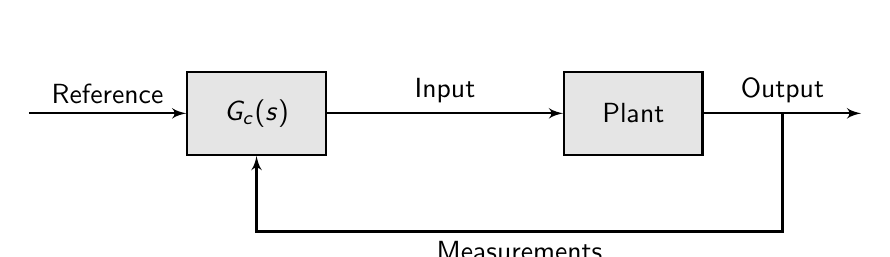
\begin{tikzpicture}[auto, node distance=2.5cm, >=latex', thick]
		% Define styles for the blocks and lines
		\tikzstyle{block} = [draw, rectangle, fill=gray!20, minimum height=3em, minimum width=5em]
		\tikzstyle{line} = [draw, ->]
		
		% Place the nodes (blocks)
		\node [block] (controller) {$G_c(s)$};
		\node [block, right=3cm of controller] (plant) {Plant};
		
		% Coordinates for start and end
		\node [coordinate, left=2cm of controller] (input) {};
		\node [coordinate, right=2cm of plant] (output) {};
		
		% Draw the connections
		% 1. Reference to G(s)
		\draw [line] (input) -- node {Reference} (controller);
		
		% 2. G(s) to Plant
		\draw [line] (controller) -- node {Input} (plant);
		
		% 3. Plant to Output
		\draw [line] (plant) -- node [name=y] {Output} (output);
		
		% 4. Feedback loop (Measurements)
		% We start from the output line, go down, go left, then up to G(s)
		\draw [line] (y.south) |- ++(0,-1.5) -| node [pos=0.25, below] {Measurements} (controller.south);
		
	\end{tikzpicture}
	\caption{The Classical Control Loop. The controller is a pre-designed dynamic block (e.g., PID) that maps error to input of the controlled system called \emph{plant}.}
	\label{fig:classic_loop}
\end{figure}

To give an example, in classical control (e.g., Proportional-Integral-Derivative or PID), the engineer explicitly defines \emph{how} the controller calculates the input. The internal structure of a PID controller is shown in Figure~\ref{fig:pid_structure}. A PID controller is explicitly instructed to:
\begin{enumerate}
	\item Calculate the error, $e(t)=r(t)-y(t)$ (Reference - Output).
	\item Integrate the error, $\int e(t)dt$.
	\item Differentiate the error, $\dfrac{d}{dt}e(t)$.
	\item Multiply these terms by specific gains ($K_p, K_i, K_d$) and sum them to obtain control signal, $$u(t)=K_pe(t)+K_i \int e(t)dt+K_d\frac{d}{dt}e(t)$$
\end{enumerate}
This sum constitutes the control input that is applied to the plant. The behaviour is fixed by the mathematical structure of the controller. That means when one knows $e(t)$ numerically and once the control gains ($K_p, K_i, K_d$) are selected, the control signal applied to the plant can be precisely calculated in closed form. 

\begin{figure}[t]
	\centering
	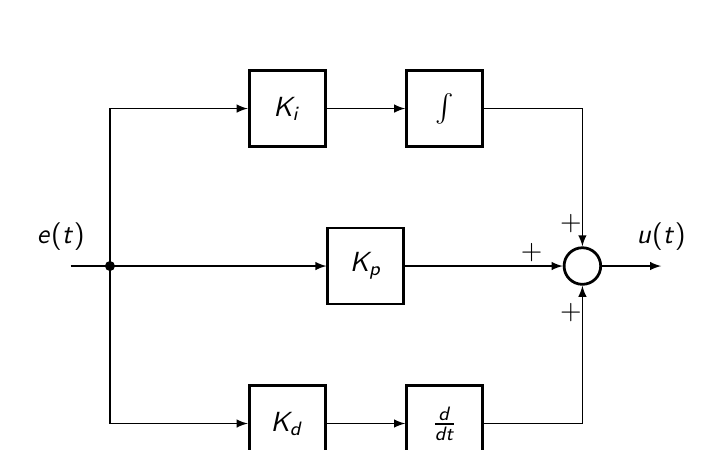
\begin{tikzpicture}
		% Paths, nodes and wires:
		\node[shape=rectangle, draw, line width=1pt, minimum width=0.965cm, minimum height=0.965cm](N1) at (4.25, 9){} node[anchor=center] at (N1.text){$K_i$};
		\node[shape=rectangle, draw, line width=1pt, minimum width=0.965cm, minimum height=0.965cm](N2) at (6.25, 9){} node[anchor=center] at (N2.text){$\int$};
		\node[shape=rectangle, draw, line width=1pt, minimum width=0.965cm, minimum height=0.965cm](N3) at (5.25, 7){} node[anchor=center] at (N3.text){$K_p$};
		\node[shape=rectangle, draw, line width=1pt, minimum width=0.965cm, minimum height=0.965cm](N4) at (4.25, 5){} node[anchor=center] at (N4.text){$K_d$};
		\node[shape=rectangle, draw, line width=1pt, minimum width=0.965cm, minimum height=0.965cm](N5) at (6.25, 5){} node[anchor=center] at (N5.text){$\frac{d}{dt}$};
		\node[shape=circle, draw, line width=1pt, minimum width=0.465cm] at (8, 7){};
		\draw[-latex] (2, 7) -- (2, 9) -- (3.75, 9);
		\draw[-latex] (4.75, 9) -- (5.75, 9);
		\draw[-latex] (6.75, 9) -- (8, 9) -- (8, 7.25);
		\draw[-latex] (1.5, 7) -- (4.75, 7);
		\draw[-latex] (5.75, 7) -- (7.75, 7);
		\draw[-latex] (2, 7) -- (2, 5) -- (3.75, 5);
		\draw[-latex] (4.75, 5) -- (5.75, 5);
		\draw[-latex] (6.75, 5) -- (8, 5) -- (8, 6.75);
		\draw[-latex] (8.25, 7) -- (9, 7);
		\node[circ] at (2, 7){};
		\node[shape=rectangle, minimum width=0.465cm, minimum height=0.715cm] at (7.75, 7.5){} node[anchor=north west, align=left, text width=0.077cm, inner sep=6pt] at (7.5, 7.875){$+$};
		\node[shape=rectangle, minimum width=0.465cm, minimum height=0.715cm] at (7.25, 7.125){} node[anchor=north west, align=left, text width=0.077cm, inner sep=6pt] at (7, 7.5){$+$};
		\node[shape=rectangle, minimum width=0.465cm, minimum height=0.715cm] at (7.75, 6.375){} node[anchor=north west, align=left, text width=0.077cm, inner sep=6pt] at (7.5, 6.75){$+$};
		\node[shape=rectangle, minimum width=0.715cm, minimum height=0.215cm](N6) at (1.375, 7.375){} node[anchor=center] at (N6.text){$e(t)$} node[anchor=north west, align=left, text width=0.327cm, inner sep=6pt] at (1, 7.5){};
		\node[shape=rectangle, minimum width=0.715cm, minimum height=0.215cm](N7) at (9, 7.375){} node[anchor=center] at (N7.text){$u(t)$} node[anchor=north west, align=left, text width=0.327cm, inner sep=6pt] at (8.625, 7.5){};
	\end{tikzpicture}
	\caption{The internal structure of a PID controller. The error ($e$) is processed in parallel: it is integrated, differentiated, and scaled by specific gains before being summed to produce the control input ($u$).}
	\label{fig:pid_structure}
\end{figure}

\subsection{The MPC Approach: Optimisation-Based Control}
As shown in Figure~\ref{fig:mpc_loop}, MPC represents a fundamental shift in this philosophy. In an MPC architecture, the explicit controller block is replaced by an \emph{optimisation routine}. Here we call it \emph{Optimiser}. This is mostly an embedded digital computer that runs an algorithm.  

Instead of specifying \emph{how} to calculate the input mathematically, MPC specifies \emph{what} the controller should achieve. That means, there is no controller structure specified but the optimiser directly generates the control signal. If the error signal, $e(t)$ is known, we do not know what the controller will generate. The signal generated by the optimiser that goes into the \emph{Plant} depends on many factors and conditions of the controller,  measured signal,  dynamics of the plant, reference signal, environmental conditions, and their current, past and predicted values. 

Generally, the engineer provides the optimiser with four key components:
\begin{enumerate}
	\item \textbf{A Model (Plant dynamics):} Information on how the plant reacts to inputs and disturbances (typically a state-space model derived from first principles like Newton's second law of motion, Kirchhoff's voltage and current laws for electrical circuits).
	\item \textbf{Measurements:} The current state $x(t)$ of the system and historical data. This could be either a measured signal or estimated one.
	\item \textbf{Objectives:} A mathematical function  \emph{cost} representing the goal (e.g., tracking a reference or minimising energy consumption).
	\item \textbf{Constraints:} Limitations on the system (e.g., maximum valve opening, safety limits, temperature limits, rate bounds of the actuator etc.).
\end{enumerate}


\begin{figure}[t]
	\centering
	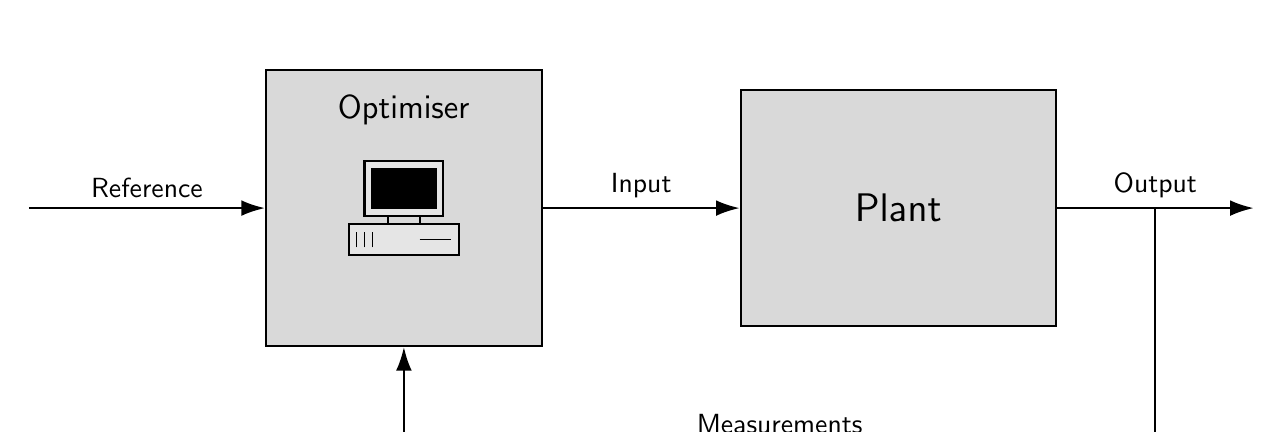
\begin{tikzpicture}[auto, node distance=2.5cm, >={Latex[length=3mm, width=2mm]}, thick]
		
		% ---------------------------------------------------------
		% 1. Define Styles
		% ---------------------------------------------------------
		\tikzstyle{block} = [draw, rectangle, fill=gray!30, minimum height=4em, minimum width=6em, text width=6em, align=center]
		\tikzstyle{line} = [draw, ->]
		\tikzstyle{coord} = [coordinate]
		
		% ---------------------------------------------------------
		% 2. Place Nodes (Blocks)
		% ---------------------------------------------------------
		
		% The Optimizer Block (We make it larger to fit the icon)
		\node [block, minimum height=3.5cm, minimum width=3.5cm] (opt) {};
		
		% Text label for Optimizer (placed at the top of the block)
		\node [below=0.2cm] at (opt.north) {\large \textsf{Optimiser}};
		
		% The Computer Icon (drawn manually inside the Optimizer block)
		% Monitor
		\draw [fill=black!10, thick] ($(opt.center)+(-0.5, -0.1)$) rectangle ($(opt.center)+(0.5, 0.6)$);
		\draw [fill=black] ($(opt.center)+(-0.4, 0.0)$) rectangle ($(opt.center)+(0.4, 0.5)$);
		% Stand
		\draw [thick] ($(opt.center)+(-0.2, -0.1)$) -- ($(opt.center)+(-0.2, -0.2)$) -- ($(opt.center)+(0.2, -0.2)$) -- ($(opt.center)+(0.2, -0.1)$);
		% PC Unit (Desktop case)
		\draw [fill=black!10, thick] ($(opt.center)+(-0.7, -0.6)$) rectangle ($(opt.center)+(0.7, -0.2)$);
		% Vents/Drive details on PC Unit
		\draw [thin] ($(opt.center)+(-0.6, -0.5)$) -- ($(opt.center)+(-0.6, -0.3)$);
		\draw [thin] ($(opt.center)+(-0.5, -0.5)$) -- ($(opt.center)+(-0.5, -0.3)$);
		\draw [thin] ($(opt.center)+(-0.4, -0.5)$) -- ($(opt.center)+(-0.4, -0.3)$);
		\draw [thin] ($(opt.center)+(0.2, -0.4)$) -- ($(opt.center)+(0.6, -0.4)$);
		
		% The Plant Block
		\node [block, right=2.5cm of opt, minimum height=3cm, minimum width=4cm] (plant) {\Large \textsf{Plant}};
		
		% ---------------------------------------------------------
		% 3. Draw Connections
		% ---------------------------------------------------------
		
		% Input Reference
		\node [coord, left=3cm of opt] (input) {};
		\draw [line] (input) -- node[above] { \textsf{Reference}} (opt);
		
		% Optimizer to Plant
		\draw [line] (opt) -- node[above] { \textsf{Input}} (plant);
		
		% Output
		\node [coord, right=2.5cm of plant] (output) {};
		\draw [line] (plant) -- node[name=y, above] { \textsf{Output}} (output);
		
		% Feedback Loop (Measurements)
		% Start from the output line 'y', go down, go left, go up into bottom of Optimizer
		\draw [line] (y.south) |- ++(0,-3) -| node[pos=0.25, above] { \textsf{Measurements}} (opt.south);
		
	\end{tikzpicture}
	\caption{The MPC Control Loop. The fixed controller is replaced by an on-line optimiser that uses a model and constraints of the plant as well as predefined objective function to solve for the optimal control input.}
	\label{fig:mpc_loop}
\end{figure}


The optimiser processes this information to select the input that brings the plant to ideal form by minimising an objective (cost) while strictly respecting constraints. 

\section{Conceptual Framework: The Racing Car Analogy}

To intuitively grasp the mechanics of MPC, consider the challenge of driving a racing car around a circuit in the minimum possible time. To design an effective controller for this vehicle, one must first formalise the environment and the vehicle’s behaviour:
\begin{itemize}
	\item \textbf{The Model (Dynamics):} The controller must understand how the car responds to inputs—how steering, acceleration, and braking translate into changes in position and velocity.
	\item \textbf{The Measurements (Feedback):} To plan the optimal trajectory, the controller must know the car's current state at every instant. This includes the position ($x, y$) relative to the track boundaries, the velocity ($v$) to judge braking distances, and the heading angle ($\theta$) to align with the apex of the next corner.
	\item \textbf{The Objective (Cost Function):} The primary goal is to minimise the lap time, often whilst secondary goals, such as minimising fuel consumption or tyre wear, are also considered.
	\item \textbf{The Constraints:} The car must remain within the track boundaries, stay below the engine's maximum power output, and respect the physical limits of tyre traction to avoid skidding.

\end{itemize}
Consider the racing track shown in Figure~\ref{fig:racing_car}. A human driver naturally performs predictive control. Upon approaching a corner, the driver does not simply react to the car's current position. Instead, they look ahead—establishing a \textit{prediction horizon}. They anticipate the car's future trajectory based on its current momentum and adjust their inputs \textit{proactively}. For example, a driver will pull to the outside of the track to flatten the turn radius, anticipating the geometry of the road ahead before they even reach the apex.

\begin{figure}[t]
	\centering
	\includegraphics[width=0.9\textwidth]{Figures/racing1.pdf}
	\caption{Model Predictive Control for trajectory optimisation in a racing scenario. The controller plans an optimal path (cyan) over the prediction horizon that minimises a cost function (tracking the reference line) while satisfying state constraints (track edges) and avoiding obstacles (red cars).}
	\label{fig:racing_car}
\end{figure}

Imagine if the driver planned the entire lap at the starting line based on a map, closed their eyes, and executed that plan blindly. This "open-loop" execution would inevitably result in a crash. This failure occurs because the internal model is never perfect. There are several reasons for this failure:
\begin{itemize}
	\item \textbf{Model Mismatch:} Tyre friction changes as the rubber heats up, or oil on the track alters the grip levels. 
	\item \textbf{Disturbances:} External factors, such as sudden wind gusts, push the car off its intended path.
	\item \textbf{Unforeseen Constraints:} A driver might round a blind corner to discover a stationary, crashed car blocking the road.
\end{itemize}
The original plan calculated at the start line cannot account for these variables. To survive, the driver must use constant visual feedback to discard the old plan and calculate a new trajectory that avoids the obstacle.
In MPC, this is known as a \textbf{receding horizon} strategy. The controller calculates an optimal sequence of actions for the entire horizon but only executes the immediate first step. A fraction of a second later, it takes a new measurement and repeats the entire optimisation. This constant re-planning makes the system robust to uncertainty and ensures the car remains on the track, even in a changing or unpredictable environment.

\section{Receding Horizon Control (RHC)}

The mathematical framework that brings the racing car analogy to life is known as \textit{Receding Horizon Control} (RHC). This strategy serves as the engine of MPC, bridging the gap between static optimisation and dynamic control.

\subsection{The Algorithm}
The RHC strategy operates in discrete time steps. At each sampling instant $t$, the controller performs the following sequence, as illustrated in Figure~\ref{fig:mpc_concept_and_timeline}:

\begin{enumerate}
	\item \textbf{Measure:} Obtain the current state of the system, denoted as $x(t)$ via sensors or estimators. This provides the \emph{starting line} for the current iteration.
	\item \textbf{Plan (Optimise):} Using an internal model of the plant, calculate an optimal sequence of future control inputs $\{u_0, u_1, \dots, u_{N-1}\}$ over a finite prediction horizon $N$. This sequence is chosen to minimise a cost function (such as error from a reference) whilst respecting all physical constraints.
	
	\item \textbf{Execute:} Although a full sequence of $N$ steps was calculated, the controller applies \textbf{only the first element}, $u_0$, to the plant. The remaining $N-1$ steps of the plan are discarded.
	\item \textbf{Evolve:} The system evolves for one sample period under the influence of the applied input and any external disturbances.
	\item \textbf{Repeat:} At the next time step $t+1$, the entire process begins again. The horizon "recedes" (shifts forward by one step), and a new optimisation problem is solved from the new state 	$x(t+1)$.
\end{enumerate}

\begin{figure}[h]
	\centering
	\resizebox{0.85\textwidth}{!}{
	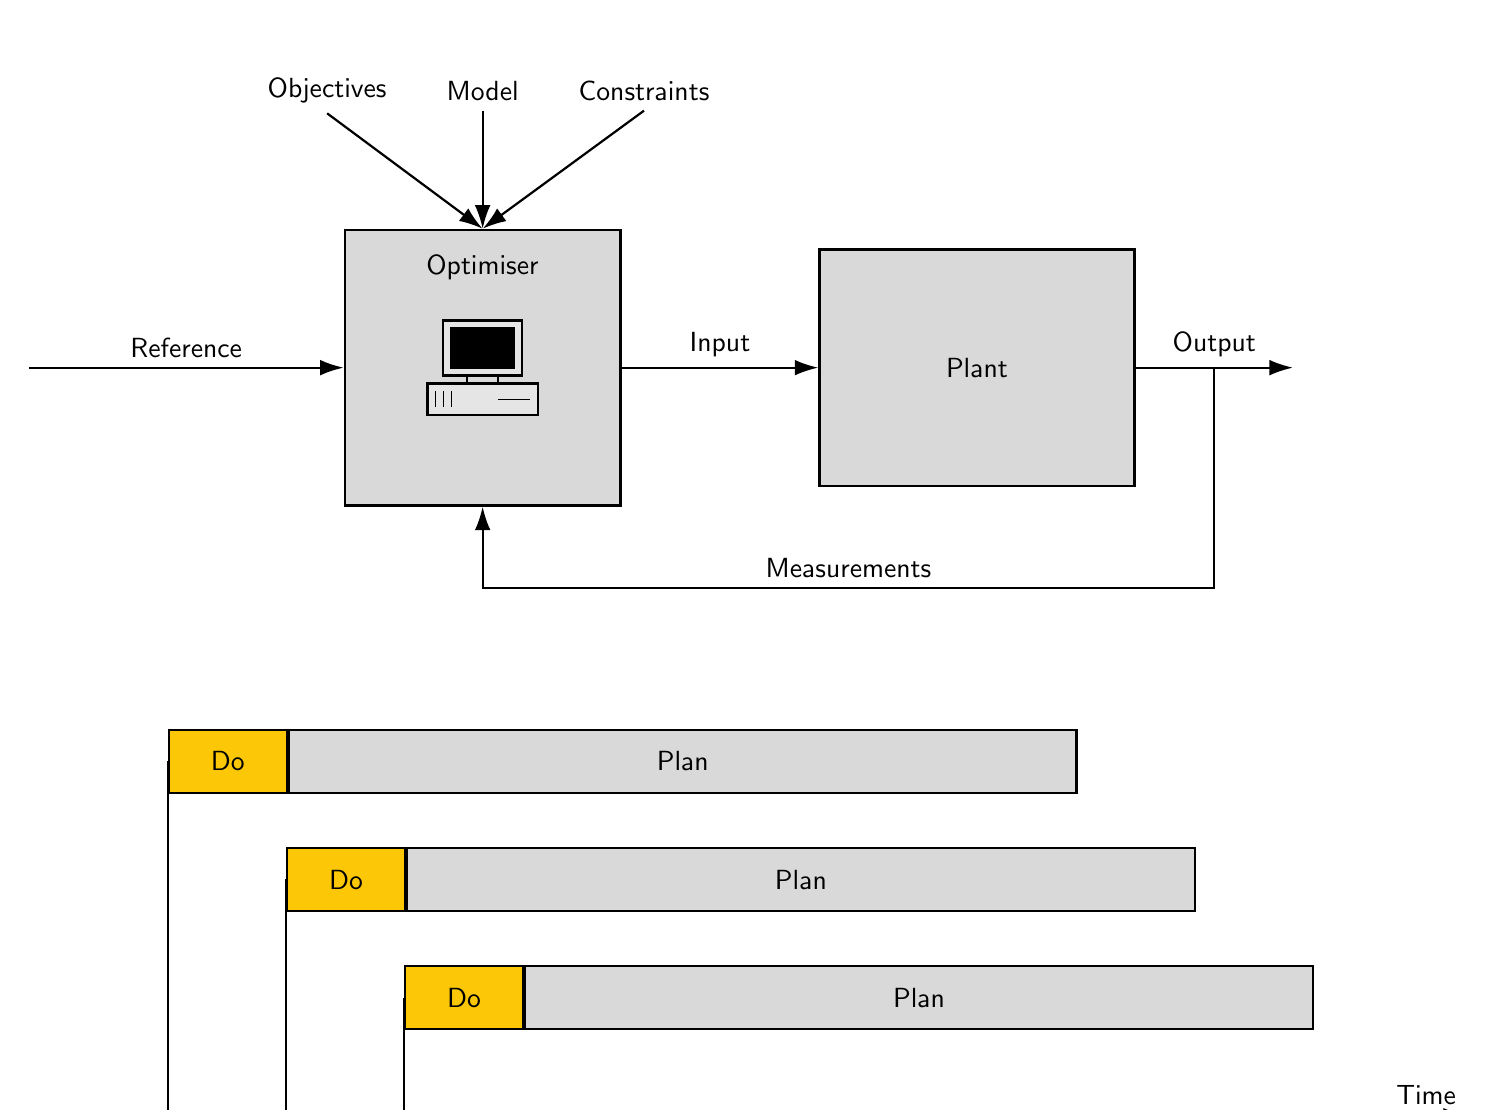
\begin{tikzpicture}[auto, >={Latex[length=3mm, width=2mm]}, thick]
		
		% =========================================================
		% PART 1: TOP DIAGRAM (CONTROL LOOP)
		% =========================================================
		
		% 1. Define Styles
		\tikzstyle{block} = [draw, rectangle, fill=gray!30, minimum height=4em, minimum width=6em, align=center]
		\tikzstyle{line} = [draw, ->]
		
		% 2. Place Main Blocks
		% Optimizer Block
		\node [block, minimum height=3.5cm, minimum width=3.5cm] (opt) at (0,0) {};
		\node [below=0.2cm] at (opt.north) { \textsf{Optimiser}};
		
		% Computer Icon inside Optimizer
		\draw [fill=black!10, thick] ($(opt.center)+(-0.5, -0.1)$) rectangle ($(opt.center)+(0.5, 0.6)$);
		\draw [fill=black] ($(opt.center)+(-0.4, 0.0)$) rectangle ($(opt.center)+(0.4, 0.5)$);
		\draw [thick] ($(opt.center)+(-0.2, -0.1)$) -- ($(opt.center)+(-0.2, -0.2)$) -- ($(opt.center)+(0.2, -0.2)$) -- ($(opt.center)+(0.2, -0.1)$);
		\draw [fill=black!10, thick] ($(opt.center)+(-0.7, -0.6)$) rectangle ($(opt.center)+(0.7, -0.2)$);
		\draw [thin] ($(opt.center)+(-0.6, -0.5)$) -- ($(opt.center)+(-0.6, -0.3)$);
		\draw [thin] ($(opt.center)+(-0.5, -0.5)$) -- ($(opt.center)+(-0.5, -0.3)$);
		\draw [thin] ($(opt.center)+(-0.4, -0.5)$) -- ($(opt.center)+(-0.4, -0.3)$);
		\draw [thin] ($(opt.center)+(0.2, -0.4)$) -- ($(opt.center)+(0.6, -0.4)$);
		
		% Plant Block
		\node [block, right=2.5cm of opt, minimum height=3cm, minimum width=4cm] (plant) { \textsf{Plant}};
		
		% 3. Main Horizontal Connections
		% Reference
		\node [coordinate, left=4cm of opt] (input) {};
		\draw [line] (input) -- node[above] { \textsf{Reference}} (opt);
		
		% Input
		\draw [line] (opt) -- node[above] { \textsf{Input}} (plant);
		
		% Output
		\node [coordinate, right=2cm of plant] (output) {};
		\draw [line] (plant) -- node[name=y, above] { \textsf{Output}} (output);
		
		% Feedback
		\draw [line] (y.south) |- ++(0,-2.8) -| node[pos=0.25, above] { \textsf{Measurements}} (opt.south);
		
		% 4. Top Inputs (Objectives, Model, Constraints)
		\node [above=1.5cm of opt] (model) { \textsf{Model}};
		\node [left=0.5cm of model] (obj) { \textsf{Objectives}};
		\node [right=0.5cm of model] (const) { \textsf{Constraints}};
		
		\draw [line] (obj.south) -- (opt.north);
		\draw [line] (model.south) -- (opt.north);
		\draw [line] (const.south) -- (opt.north);
		
		
		% =========================================================
		% PART 2: BOTTOM DIAGRAM (TIMELINE)
		% =========================================================
		
		% Shift coordinate system down
		\begin{scope}[yshift=-8cm, xshift=-4cm]
			
			% Styles for bars
			\tikzstyle{dobar} = [draw, fill=yellow!80!red, minimum height=0.8cm]
			\tikzstyle{planbar} = [draw, fill=gray!30, minimum height=0.8cm, anchor=west]
			
			% Row 1 (Top)
			\node [dobar, minimum width=1.5cm, anchor=west] (do1) at (0, 3) { \textsf{Do}};
			\node [planbar, minimum width=10cm] (plan1) at (do1.east) { \textsf{Plan}};
			% Vertical line to axis
			\draw [thick] (do1.west) -- (0, 0);
			
			% Row 2 (Middle) - Shifted right
			\node [dobar, minimum width=1.5cm, anchor=west] (do2) at (1.5, 1.5) { \textsf{Do}};
			\node [planbar, minimum width=10cm] (plan2) at (do2.east) { \textsf{Plan}};
			% Vertical line to axis
			\draw [thick] (do2.west) -- (1.5, 0);
			
			% Row 3 (Bottom) - Shifted right again
			\node [dobar, minimum width=1.5cm, anchor=west] (do3) at (3.0, 0) {}; % Empty box for alignment initially
			% Re-draw slightly offset to look "stacked" properly or just place nodes manually
			% Let's place explicitly to match image structure
			\node [dobar, minimum width=1.5cm, anchor=west] (do3_real) at (3.0, 0) { \textsf{Do}};
			\node [planbar, minimum width=10cm] (plan3) at (do3_real.east) { \textsf{Plan}};
			% Vertical line to axis
			\draw [thick] (do3_real.west) -- (3.0, -1.5); % Extend down to axis
			
			% Time Axis
			\draw [->, very thick] (-0.5, -1.5) -- (16.5, -1.5) node[above left] { \textsf{Time}};
			
			% Fix vertical lines for Row 1 and 2 to reach the new axis level
			\draw [thick] (do1.west) -- (0, -1.5);
			\draw [thick] (do2.west) -- (1.5, -1.5);
			
		\end{scope}
		
	\end{tikzpicture}
}
	\caption{\textbf{Top}: The closed-loop architecture. The controller uses an internal Model to predict plant behaviour, an Optimiser to minimise a cost function (Objectives) subject to safety limits (Constraints), and real-time Measurements to correct prediction errors.
		\textbf{Bottom}: The Receding Horizon strategy. At each time step, an optimal trajectory is computed over a long prediction horizon (\emph{Plan}), but only the first control action is applied (\emph{Do}). The horizon then shifts forward, and the optimisation repeats with updated feedback, turning an open-loop prediction into a closed-loop controller.}
	\label{fig:mpc_concept_and_timeline}
\end{figure}

The reader may naturally ask: \textit{"If the plan calculated at step $t$ was \emph{optimal}, why discard the rest of it and repeat the work at step $t+1$?"}

The answer lies in the inevitable gap between the controller's internal model and the real world. If we were to execute the entire $N$-step sequence without looking back, we would be operating in \emph{open-loop}. Any small modelling error that falls into that $N$ instants or unexpected gust of wind would cause the system to drift away from the intended path.

By only executing the first step and then re-measuring the state, we turn a series of open-loop predictions into a \emph{closed-loop} feedback strategy. The \emph{horizon} refers to how far into the future the controller predicts. Since we repeat the optimisation at every step, the horizon moves forward with time. This repetitive re-planning ensures that the control action is always based on the most current information. The \emph{receding} nature of the horizon ensures that the controller is constantly correcting for errors and reacting to new information, much like the driver who constantly adjusts their steering as the road unfolds. 

\section{Why Use Model Predictive Control?}

Whilst traditional control methods—like Proportional-Integral-Derivative (PID) control, lead-lag compensation, and the Linear Quadratic Regulator (LQR)—are still workhorses of industrial automation, they often hit their limits when dealing with today's demanding performance requirements. Model Predictive Control has become a leading approach for complex systems by anticipating future behaviour through model-based prediction.

The transition from classical methods to MPC is typically driven by the need to operate closer to the physical limits of a system without compromising safety or stability. Unlike traditional controllers, which are often tuned via trial-and-error to achieve a specific response, MPC provides a systematic framework that accounts for the system's model and its environment. The primary advantages that distinguish MPC from its predecessors are outlined in the following subsections.

\subsection{Systematic Handling of Constraints}

This is the most significant advantage of MPC. In the real world, every engineering system is subject to physical and operational limits. These may include \textit{actuator constraints}, such as the maximum opening of a valve or the voltage limit of a motor, and \textit{state constraints}, such as maintaining a chemical reactor below a critical temperature or ensuring a vehicle remains within track boundaries.

\textbf{Classical Control:} Ignores constraints during design and is inherently \emph{blind} to these boundaries. A PID controller, for instance, may calculate a control action that the hardware cannot physically execute. This often leads to \emph{integrator windup}, where the controller's internal logic becomes saturated, resulting in large overshoots or sluggish recovery. 

\textbf{MPC:} Includes constraints directly in the optimisation. The optimiser knows the limits and will find the best control action that resides \textit{on the boundary} of those limits without crossing them. MPC behaves non-linearly: it acts gently when far from a constraint but aggressively when approaching a limit to prevent violation. (See Figure~\ref{fig:constraints_comparison}). MPC treats constraints as fundamental components of the control problem. By predicting future behaviour, the optimiser can anticipate a potential constraint violation and adjust the control signal proactively \emph{before} the limit is reached. This ability to operate safely at the very edge of the feasible operating space is perhaps the most significant economic driver for MPC in industry.


\begin{figure}[h]
	\centering
	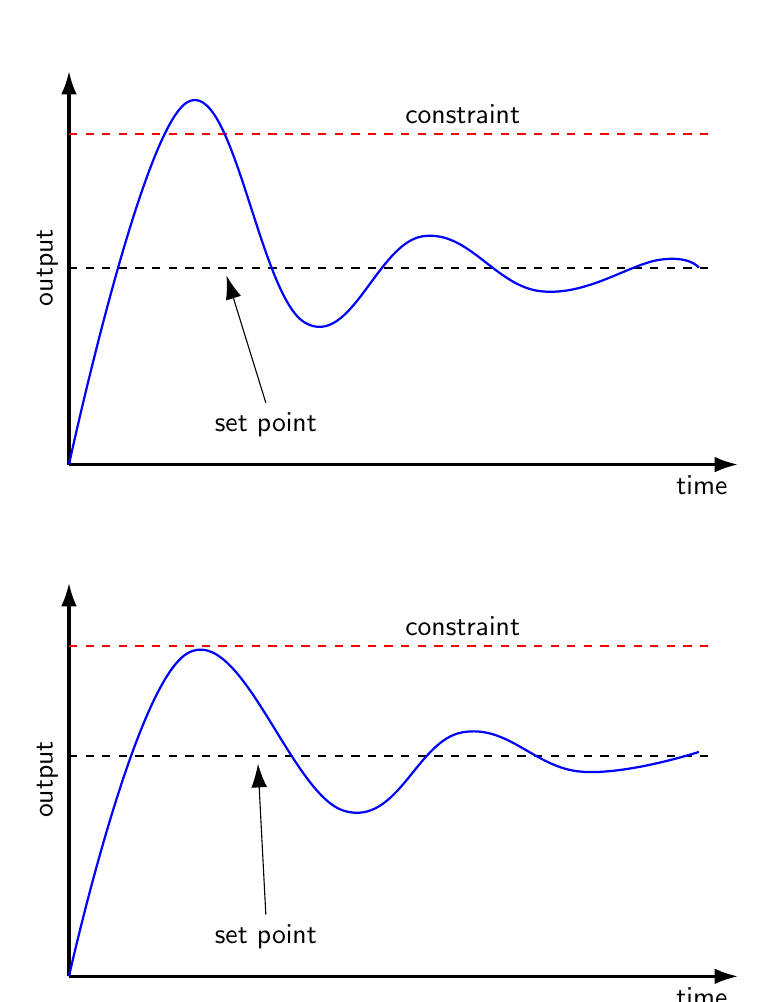
\begin{tikzpicture}[>={Latex[length=3mm, width=2mm]}, thick, font=\sffamily]
		
		% ---------------------------------------------------------
		% TOP PLOT: Violation of Constraint
		% ---------------------------------------------------------
		\begin{scope}
			% Axes
			\draw[->, very thick] (0,0) -- (8.5,0) node[below left] { time};
			\draw[->, very thick] (0,0) -- (0,5) node[midway, above, rotate=90] { output};
			
			% Constraint Line (Red Dashed)
			\draw[red, dashed, thick] (0,4.2) -- (8.2,4.2);
			\node[above] at (5, 4.2) { constraint};
			
			% Set Point Line (Black Dashed)
			\draw[dashed, thick] (0,2.5) -- (8.2,2.5);
			
			% The Response Curve (Blue) - High Overshoot
			% Using coordinates to shape the "Underdamped" look
			\draw[blue, thick] plot [smooth, tension=0.7] coordinates {
				(0,0) 
				(1.5, 4.6)   % Peak crossing constraint
				(3.0, 1.8)   % Valley
				(4.5, 2.9)   % Secondary Peak
				(6.0, 2.2)   % Secondary Valley
				(7.5, 2.6)   % Settling
				(8.0, 2.5)
			};
			
			% Set Point Label
			\node (sp_text) at (2.5, 0.5) { set point};
			\draw[->, thin] (sp_text.north) -- (2.0, 2.4);
		\end{scope}
		
		% ---------------------------------------------------------
		% BOTTOM PLOT: Respecting Constraint (MPC Style)
		% ---------------------------------------------------------
		\begin{scope}[yshift=-6.5cm] % Shift down
			% Axes
			\draw[->, very thick] (0,0) -- (8.5,0) node[below left] { time};
			\draw[->, very thick] (0,0) -- (0,5) node[midway, above, rotate=90] { output};
			
			% Constraint Line (Red Dashed)
			\draw[red, dashed, thick] (0,4.2) -- (8.2,4.2);
			\node[above] at (5, 4.2) { constraint};
			
			% Set Point Line (Black Dashed)
			% Note: In the image, the bottom set point looks slightly higher relative to the axis
			\draw[dashed, thick] (0,2.8) -- (8.2,2.8);
			
			% The Response Curve (Blue) - Controlled Overshoot
			\draw[blue, thick] plot [smooth, tension=0.7] coordinates {
				(0,0) 
				(1.5, 4.1)   % Peak just below constraint
				(3.5, 2.1)   % Valley
				(5.0, 3.1)   % Secondary Peak
				(6.5, 2.6)   % Secondary Valley
				(8.0, 2.85)  % Settling
			};
			
			% Set Point Label
			\node (sp_text_b) at (2.5, 0.5) { set point};
			\draw[->, thin] (sp_text_b.north) -- (2.4, 2.7);
		\end{scope}
		
	\end{tikzpicture}
	\caption{\textbf{Top:} Classical control showing significant overshoot violating constraints. \textbf{Bottom:} Predictive control respecting constraints by adjusting the trajectory.}
	\label{fig:constraints_comparison}
\end{figure}

\subsection{Future Knowledge and Preview Capability}

A major drawback of many traditional controllers is that they're inherently \textit{causal}—they can only react to what's already happened or what's happening right now. However, in many modern engineering applications, we often have access to "future knowledge"—information about upcoming changes in what we want the system to do, or predicted external disturbances. MPC can exploit this information directly through its prediction mechanism, via its \textit{look-ahead} or \textit{preview} capability.

To show the advantage of acting on future information, consider the following examples:
\begin{itemize}
	\item \textbf{Smart Energy Management:} Think about a building's HVAC (Heating, Ventilation, and Air Conditioning) system. If the weather forecast predicts a scorching heatwave for the afternoon—right when electricity prices hit their peak—an MPC controller can choose to "pre-cool" the building's thermal mass during the cooler morning hours whilst energy is cheaper. A traditional PID controller, being reactive, would only ramp up the cooling once the internal temperature had already started to climb, consuming electricity during the most expensive tariff period.
	
	\item \textbf{Autonomous Path Following:} In autonomous driving, the vehicle often has map data or sensor information about the road layout ahead. If there's a sharp bend coming up, a reactive controller (like a lane-keeping PID) would only start to steer or slow down once it detects a tracking error at the corner. In contrast, MPC sees the curve in its prediction horizon and begins adjusting the steering angle and reducing speed \textit{before} entering the turn. This produces a smoother, safer, and more "human-like" driving experience.
	
	\item \textbf{Renewable Energy Integration:} In a microgrid, if the forecast shows a sudden drop in solar irradiance coming (say, due to approaching cloud cover), MPC can proactively fire up a backup power source or dial back non-essential loads. This keeps the grid stable by making up for the power shortfall before the frequency actually drops.
\end{itemize}

Incorporating forecast information into the optimisation converts a reactive control strategy into a proactive one.

\subsection{Multivariable Control and Complex Objectives}

Whilst classical control theory typically tackles problems by designing individual loops for individual variables (Single-Input Single-Output, or SISO), modern systems are rarely this straightforward. MPC handles Multi-Input Multi-Output (MIMO) systems natively through its state-space formulation, and its flexibility in defining what "optimal" performance actually means.

\subsubsection{Handling Cross-Coupling in MIMO Systems}
In many real-world systems, the inputs and outputs are "coupled". This means that tweaking one input to control a particular output will inevitably affect other outputs as well. MPC handles this problem very well. 

\begin{examplebox}{The Shower Analogy.}
	Consider the everyday challenge of adjusting a shower. You've got two goals: keeping the water at a specific temperature and achieving your desired flow pressure. You also have two controls at your disposal: the hot tap and the cold tap.
	
	\begin{itemize}
		\item \textbf{The PID Approach (Decentralised):} A traditional strategy might assign one controller to temperature (operating the hot tap) and another to pressure (operating the cold tap). If you want more pressure, the pressure controller opens the cold tap. This increases the flow, but immediately throws off the temperature, causing the water to go freezing cold. The temperature controller then scrambles to fix this, which in turn messes with the pressure. The two loops end up fighting each other, leading to an oscillation and a rather uncomfortable shower.
		
		\item \textbf{The MPC Approach (Centralised):} MPC uses a multivariable model that understands how everything interacts. It knows that to increase pressure \textit{without} disturbing the temperature, it needs to open \textit{both} the hot and cold taps at the same time in just the right ratio. Because it works out all the inputs together, it accounts for cross-coupling automatically—no need for complicated decoupling networks.
	\end{itemize}
\end{examplebox}

\subsubsection{Defining \emph{Optimality} via Cost Functions}

Classical controllers such as PID typically have a very narrow notion of what constitutes success: the control objective is simply to drive the tracking error to zero. While this makes PID controllers effective and easy to deploy, it also means that they have no inherent understanding of \emph{cost} or \emph{trade-offs}. Model Predictive Control (MPC), by contrast, is built around an explicit cost function, denoted by \(J\), which allows the engineer to state mathematically what aspects of performance are important for a given application.

By tuning the relative \emph{weights} of the different terms in the cost function, the behaviour of an MPC controller can be shaped to handle more complex and realistic scenarios, where competing objectives must be balanced rather than optimised in isolation.

Consider, for example, a high-precision servo system. A PID controller may react very aggressively in its attempt to eliminate even tiny tracking errors, leading to rapid actuator motion and unwanted vibrations. An MPC controller can be designed to include a penalty on the \emph{rate of change} of the control input, \(\Delta u\). This effectively tells the controller to prioritise accurate tracking, but only insofar as it does not require excessive or abrupt actuation. The resulting control signal is smoother, reducing mechanical wear and helping to extend the lifespan of the hardware.

A similar principle applies in process control applications such as chemical plants. There may be several different ways to achieve the desired product quality. One strategy might rely more heavily on steam, which is effective but expensive, while another might use additional catalyst, which is cheaper but leads to slower dynamics. Within an MPC framework, such preferences can be encoded directly by assigning different economic weights to each input. The optimiser then determines the specific combination of control actions that satisfies the quality constraints while minimising the overall financial cost.



\section{Operation of MPC}

The Model Predictive Control problem is fundamentally defined as a finite-horizon optimisation problem that is solved repeatedly at each time step. To understand how MPC operates, one must examine its three core mathematical components: Modelling the cost function, imposing constraints, and applying the receding horizon principle.

\subsection{The Prediction Model}
Predicting the future evolution of a system requires an explicit mathematical description of its dynamics. As digital controllers operate at discrete sampling instants, this description is typically expressed in discrete time. For a linear, time-invariant system, the prediction model is written in State–Space form as
\begin{equation}
	x_{k+1} = A x_k + B u_k .
\end{equation}
Here, $x_k \in \mathbb{R}^n$ denotes the \emph{state vector}, which encapsulates the variables describing the system’s current condition (such as position, velocity, or temperature), while $u_k \in \mathbb{R}^m$ denotes the \emph{control input} applied at time step $k$. The matrices $A$ and $B$ characterise the system dynamics and determine how the state evolves from time step $k$ to $k+1$ under the applied input.

\subsection{The Objective (Cost Function)}
With a model capable of predicting future behaviour, the next step is to define what constitutes desirable performance. In MPC, this is achieved through the definition of a scalar cost function, $J$, which evaluates the quality of a predicted state and input trajectory over a finite prediction horizon of length $N$. A widely adopted choice is the quadratic cost function
\begin{equation}
	J(x_0, {u}) = \sum_{k=0}^{N-1} \left( x_k^\top  Q x_k + u_k^\top  R u_k \right) + x_N^\top  Q_N x_N .
\end{equation}
\begin{notebox}{Cost function scaling}
Some references (and Chapter~5) include a factor $\tfrac{1}{2}$ in front of the cost for compatibility with the standard QP form $\tfrac{1}{2}z^\top H z + f^\top z$. This does not change the optimal solution --- only the numerical value of the cost. We omit the $\tfrac{1}{2}$ here for clarity.
\end{notebox}
The quadratic structure ensures that larger deviations are penalised disproportionately more than smaller ones, reflecting a least-squares philosophy. The relative importance of competing objectives is governed by the weighting matrices:
\begin{itemize}
	\item \textbf{Performance weight ($Q$):} penalises deviations of the state from its reference. Increasing $Q$ encourages faster error correction and leads to more aggressive closed-loop behaviour.
	\item \textbf{Input weight ($R$):} penalises control effort. Larger values of $R$ discourage excessive or rapid changes in the control input, resulting in more conservative actuation.
	\item \textbf{Terminal weight ($Q_N$):} penalises the terminal state $x_N$ at the end of the horizon and is commonly introduced to promote stability and desirable long-term behaviour.
\end{itemize}

Although the compact matrix notation $x^\top  Q x$ is mathematically convenient, it can obscure the physical interpretation of the tuning parameters. To clarify this intuition, it is instructive to examine a simple example.

Consider a mechanical system, such as a robotic manipulator or a vehicle, with two state variables and a single control input:
\begin{itemize}
	\item $x_1$: position error relative to a desired target,
	\item $x_2$: velocity,
	\item $u$: applied force (for example, motor voltage or throttle input).
\end{itemize}
The state vector is therefore $x_k = \begin{bmatrix} x_1 \\ x_2 \end{bmatrix}$. In practice, the state weighting matrix $Q$ is almost always chosen to be diagonal, allowing each state component to be penalised independently:
\begin{equation}
	Q = \begin{bmatrix} q_1 & 0 \\ 0 & q_2 \end{bmatrix} ,
\end{equation}
where $q_1 \ge 0$ and $q_2 \ge 0$ are tuning parameters selected by the engineer.

\subsubsection*{Explicit Expansion of the Cost}
Expanding the quadratic term $x_k^\top  Q x_k$ reveals its interpretation as a weighted sum of squared state variables:
\begin{equation}
	\begin{aligned}
		x_k^\top  Q x_k 
		&= \begin{bmatrix} x_1 & x_2 \end{bmatrix}
		\begin{bmatrix} q_1 & 0 \\ 0 & q_2 \end{bmatrix}
		\begin{bmatrix} x_1 \\ x_2 \end{bmatrix} \\
		&= \begin{bmatrix} x_1 & x_2 \end{bmatrix}
		\begin{bmatrix} q_1 x_1 \\ q_2 x_2 \end{bmatrix} \\
		&= q_1 x_1^2 + q_2 x_2^2 .
	\end{aligned}
\end{equation}
Each state therefore contributes to the overall cost in proportion to both its magnitude and its associated weight. If the control input is scalar, the matrix $R$ reduces to a single non-negative scalar $r$, and the corresponding term simplifies to
\begin{equation}
	u_k^\top  R u_k = r u_k^2 .
\end{equation}
This formulation highlights that MPC does not merely seek to eliminate state error, but instead explicitly balances tracking performance against the cost of control effort.


\subsubsection*{How to Tune the Weights}
Once the cost function is written out explicitly, its interpretation becomes quite intuitive. In essence, $J$ acts like a balance sheet: at every time step, the controller adds up a set of penalties and then chooses the control action that makes this total as small as possible:
\begin{equation}
	J \approx \sum \big( \underbrace{q_1 x_1^2}_{\text{Position penalty}} 
	+ \underbrace{q_2 x_2^2}_{\text{Velocity penalty}} 
	+ \underbrace{r u^2}_{\text{Energy penalty}} \big) .
\end{equation}
The relative size of the weights determines the controller’s priorities and, ultimately, its behaviour. Several typical tuning regimes are worth highlighting:

\begin{enumerate}
	\item \textbf{High-precision tuning ($q_1 \gg r$):}  
	If, for instance, $q_1 = 100$ and $r = 1$, the controller treats position errors as far more costly than the use of control effort. As a result, it will act aggressively, applying large inputs to eliminate even small position errors as quickly as possible.
	
	\item \textbf{Energy-saving tuning ($r \gg q_1$):}  
	Conversely, if $r = 100$ and $q_1 = 1$, control effort is considered expensive. In this case, the controller is willing to tolerate larger or longer-lasting position errors if that reduces the amount of energy or fuel consumed.
	
	\item \textbf{Damping-oriented tuning (large $q_2$):}  
	If the closed-loop response exhibits excessive oscillations, increasing $q_2$ can be effective. Since $x_2$ represents velocity, heavily penalising this term discourages rapid motion, resulting in a smoother, more heavily damped response that behaves much like an electronic damper.
\end{enumerate}


Thus, $Q$ and $R$ are not abstract mathematical abstractions; they are the \emph{knobs} the engineer turns to define the personality of the controller.

\subsection{Constraint Handling}

Unlike classical control approaches (such as PID), which may effectively demand unbounded actuation without regard for physical feasibility, MPC is formulated to explicitly respect real-world limitations. The optimisation problem is therefore solved subject to a set of constraints, typically expressed as linear inequalities. In compact matrix form, these constraints are written as
\begin{equation}
	F x_k + G u_k \leq b .
\end{equation}
At first glance, this expression may appear rather abstract. In practice, however, it is nothing more than a convenient way of collecting many simple and intuitive rules into a single mathematical statement. Each row of the inequality corresponds to a specific restriction—such as limits on actuator saturation, allowable state ranges, or safety margins—that the controller is required to satisfy at every time step.


\begin{examplebox}{Constraints always exist in physical systems}
Let us revisit our 2-state vehicle system, where $x_1$ is position, $x_2$ is velocity, and $u$ is the acceleration command. Suppose we have the following physical limits:
\begin{enumerate}
	\item \textbf{Actuator Limit:} The engine can provide a maximum acceleration of $+10 \, m/s^2$ and a maximum braking (deceleration) of $-10 \, m/s^2$.
	\item \textbf{Safety Limit:} The vehicle must not exceed a speed limit of $50 \, m/s$.
\end{enumerate}

Mathematically, these are three separate inequalities:
\begin{align*}
	u_k &\leq 10 && \text{(Max Accel)} \\
	u_k &\geq -10 \implies -u_k \leq 10 && \text{(Max Brake - note the sign flip)} \\
	x_2 &\leq 50 && \text{(Speed Limit)}
\end{align*}
\textit{Note:} Standard solvers usually require all constraints to be in the form "$\dots \leq \text{Constant}$". Therefore, we multiply "greater than" constraints by $-1$ to flip the sign.

To fit these into the standard form $F x_k + G u_k \leq b$, we stack them into matrices. Recall that $x_k = [x_1, x_2]^\top $:

\begin{equation}
	\underbrace{
		\begin{bmatrix}
			0 & 0 \\
			0 & 0 \\
			0 & 1
		\end{bmatrix}
	}_{F}
	\begin{bmatrix} x_1 \\ x_2 \end{bmatrix}
	+
	\underbrace{
		\begin{bmatrix}
			1 \\
			-1 \\
			0
		\end{bmatrix}
	}_{G}
	u_k
	\leq
	\underbrace{
		\begin{bmatrix} 
			10 \\
			10 \\
			50 
		\end{bmatrix}
	}_{b}
\end{equation}

By reading this matrix row by row, we can see how the algebra represents the physical reality:
\begin{itemize}
	\item \textbf{Row 1:} $0 \cdot x + 1 \cdot u \leq 10 \implies u \leq 10$.
	\item \textbf{Row 2:} $0 \cdot x - 1 \cdot u \leq 10 \implies -u \leq 10 \implies u \geq -10$.
	\item \textbf{Row 3:} $1 \cdot x_2 + 0 \cdot u \leq 50 \implies x_2 \leq 50$.
\end{itemize}

This matrix formulation defines a \textbf{feasible region}—a geometric \emph{safe space} within which the system must operate. If the predicted trajectory tries to leave this space (e.g., predicting a velocity of $51 \, m/s$), the optimiser will actively alter the input $u_k$ to prevent the violation, ensuring the car slows down \textit{before} it breaks the speed limit.
\end{examplebox}



\begin{figure}[h]
	\centering
	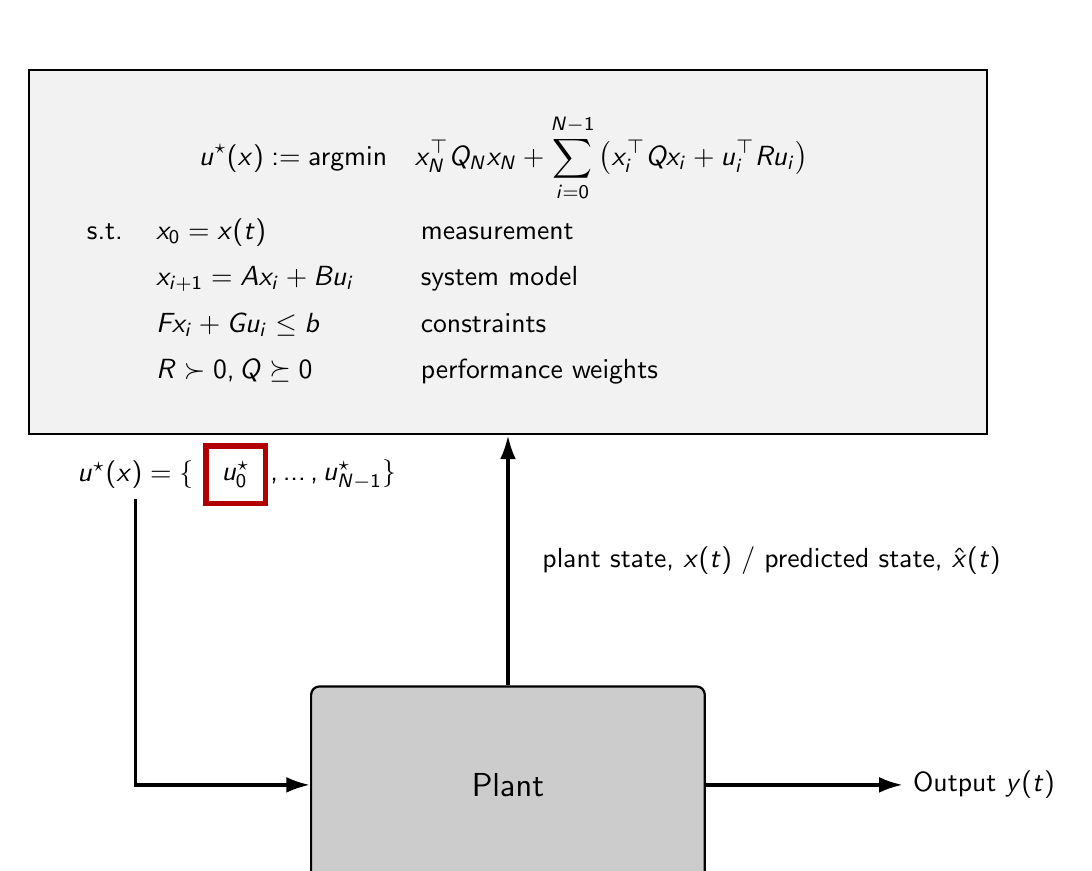
\begin{tikzpicture}[>={Latex[length=3mm, width=2mm]}, thick, font=\sffamily]

		% ---------------------------------------------------------
		% 1. TOP BLOCK: The Optimization Problem
		% ---------------------------------------------------------
		\node [draw, fill=black!5, rectangle, inner sep=15pt, align=left] (optim) {
			% We use a minipage to hold the math structure
			\begin{minipage}{11cm}
				% The Objective Function
				\begin{equation*}
					u^\star(x) := \text{argmin} \quad x_N^\top  Q_N x_N + \sum_{i=0}^{N-1} \left( x_i^\top  Q x_i + u_i^\top  R u_i \right)
				\end{equation*}
				
				% The Constraints (using a tabular for alignment)
				\vspace{-0.5em}
				\renewcommand{\arraystretch}{1.4} % Add vertical space between rows
				\begin{tabular}{rlll}
					s.t. &  $x_0 = x(t)$ & &  measurement \\
					&  $x_{i+1} = A x_i + B u_i$ & &  system model \\
					&  $F x_i + G u_i \leq b$ & &  constraints \\
					&  $R \succ 0, Q \succeq 0$ & &  performance weights
				\end{tabular}
			\end{minipage}
		};
		
		% ---------------------------------------------------------
		% 2. THE PLANT BLOCK
		% ---------------------------------------------------------
		% Positioned below and slightly to the right
		\node [draw, fill=black!20, rectangle, minimum height=2.5cm, minimum width=5cm, rounded corners=3pt, below=5.5cm of optim] (plant) at (optim.center) {\large Plant};
		
		% ---------------------------------------------------------
		% 3. THE CONTROL SEQUENCE (u*)
		% ---------------------------------------------------------
		% We split this into nodes to circle the u_0 term easily
		
		% The left part "u*(x) = {"
			\node [below=0.5cm of optim.south west, anchor=west, xshift=0.5cm] (seq_left) { $u^\star(x) = \{$};
			
			% The term to be circled "u*_0"
			\node [right=0.1cm of seq_left] (u0) { $u_0^\star$};
			
			% The Red Circle
			\node[draw=red!70!black, line width=2pt, inner sep=2pt, fit=(u0)] (square) {};
			
			
			% The rest ", ..., u*_N-1 }"
		\node [right=0.0cm of u0] (seq_right) { $, \dots, u_{N-1}^\star \}$};
		
		% ---------------------------------------------------------
		% 4. CONNECTIONS
		% ---------------------------------------------------------
		
		% Feedback Arrow: Plant -> Optimization (state x)
		% Starts from top of plant, goes to bottom of Optimization box
		\draw [->, line width=1.2pt] (plant.north) -- (plant.north |- optim.south) node [midway, right=0.3cm] { plant state,  $x(t)$ / predicted state, $\hat x(t)$};
		
		% Control Input Arrow: From the sequence to the Plant
		% Following the visual style: Line goes down from the sequence area, then right into the plant
		\draw [->, line width=1.2pt] (seq_left.south) |- (plant.west);
		
		% Output Arrow: Plant -> Output y
		\node [right=2.5cm of plant] (output) { Output $y(t)$};
		\draw [->, line width=1.2pt] (plant.east) -- (output.west);
		
	\end{tikzpicture}
	\caption{Mathematical formulation of the MPC problem and the Receding Horizon implementation.}
	\label{fig:mpc_math_formulation}
\end{figure}

\subsection{The Receding Horizon Principle}

The final piece of the MPC puzzle is the strategy of implementation. As illustrated in Figure~\ref{fig:mpc_math_formulation}, and shown in the flow chart Figure~\ref{fig:rhc_flowchart}, the process operates in closed loop, but still relying on an open-loop anticipation.

At every specific time step $t$, the controller solves the optimisation problem to find the optimal \textbf{sequence} of future control inputs, denoted as ${U}^\star$:
\begin{equation}
	{U}^\star = \{u^\star_{0}, u^\star_{1}, \dots, u^\star_{N-1}\} = \arg \min_{{U}} J(x_0, {U})
\end{equation}
This sequence represents a complete plan for the next $N$ time steps. For example, in a self-driving car, this sequence might represent the steering angles for the next 10 seconds. However,  MPC does \textbf{not} implement the entire plan but follows the following rules:

\begin{enumerate}
	\item \textbf{Extract:} Take only the first element of the optimal sequence, $u^\star_{0}$.
	\item \textbf{Apply:} Send this single signal to the plant actuators.
	\item \textbf{Discard:} Throw away the remaining calculated inputs ($u^\star_{1} \dots u^\star_{N-1}$).
	\item \textbf{Evolve:} Wait for one sample step ($t \to t+1$), measure the new state $x_{t+1}$, and shift the horizon forward by one step.
	\item \textbf{Repeat:} Solve the entire optimisation problem again from scratch.
\end{enumerate}


% Define block styles for the flowchart
\tikzstyle{block} = [rectangle, draw, fill=blue!10, 
text width=8em, text centered, rounded corners, minimum height=3em]
\tikzstyle{cloud} = [ellipse, draw, fill=red!10, 
text width=4em, text centered, minimum height=2.5em]
\tikzstyle{line} = [draw, -latex', thick]

\begin{figure}[htbp]
	\centering
	\begin{tikzpicture}[node distance=2.5cm, auto]
		
		% Nodes
		\node [block] (solve) {\textbf{Solve} optimisation problem};
		\node [block, below of=solve] (extract) {\textbf{Extract} $u^\star_{0}$};
		\node [block, below of=extract] (apply) {\textbf{Apply} to plant actuators};
		\node [cloud, below of=apply] (plant) {Plant};
		\node [block, below of=plant] (evolve) {\textbf{Evolve} $t \to t+1$ \\ Measure $x_{t+1}$};
		
		% Position the Shift node to the right of Apply
		\node [block, right of=apply, node distance=5cm] (shift) {\textbf{Shift} horizon forward};
		
		% Position the Discard node to the left of Plant
		\node [block, left of=plant, node distance=4cm] (discard) {\textbf{Discard} $u^\star_{1} \dots u^\star_{N-1}$};
		
		% Paths
		\path [line] (solve) -- (extract);
		\path [line] (extract) -- node [right] {$u^\star_0$} (apply);
		\path [line] (apply) -- (plant);
		\path [line] (plant) -- node [right] {$x_{t+1}$} (evolve);
		\path [line] (evolve) -| (shift);
		\path [line] (shift) |- (solve);
		
		% Discard arrow from extract (dashed)
		\path [line, dashed] (extract) -| node [above, pos=0.2] {unused} (discard);
		
	\end{tikzpicture}
	
	\caption{Summary of the Receding Horizon Control (RHC) loop.}
	\label{fig:rhc_flowchart}
\end{figure}
The reader might ask: \textit{"Why waste computational power calculating $N$ steps if we only use the first?"}

The answer is \textbf{feedback}. The model used for prediction is never a perfect representation of reality. If we applied the entire sequence ${U}^\star$ blindly, any unmodelled disturbance (e.g., a gust of wind) or parameter mismatch (e.g., a change in friction) would cause the system to drift off course. By re-planning at every single time step based on fresh measurements, MPC converts an "open-loop optimal control" problem into a "closed-loop feedback" strategy, ensuring robustness against uncertainty.

\vspace{0.5cm}
\begin{notebox}{Practical Guideline: When to use MPC?}
	MPC comes at a cost: it requires a mathematical model and significant computational power to solve the optimisation problem in real-time (often within milliseconds). Therefore, 
	\begin{itemize}
		\item If a system is simple (SISO), linear, and operates far from its physical limits, a classical \textbf{PID controller} is computationally cheaper and often sufficient.
		\item MPC should be reserved for problems where its unique ability to handle \textbf{constraints}, \textbf{multivariable interactions}, and \textbf{future look-ahead} justifies the added complexity.
	\end{itemize}
\end{notebox}

\section{Applications of Model Predictive Control}

Model Predictive Control (MPC) is widely used across an exceptionally broad
range of application domains. One of its distinguishing characteristics is
its scalability across vastly different time scales. Nowadays, it is applied to different systems ranging from nanoseconds in embedded electronic systems to weeks in large-scale industrial and logistical decision-making. This diversity reflects MPC’s ability to exploit predictions, incorporate  constraints, and handle multivariable interactions in a unified framework.

\subsubsection*{Nanosecond to Millisecond Domains}

At the fastest end of the spectrum, MPC is deployed in
\begin{itemize}
	\item \textbf{Computer control (ns scale)}, where extremely rapid
	decision-making is required, for example in advanced semiconductor
	manufacturing or embedded hardware processes.
	
	\item \textbf{Traction control (ms scale)}, where vehicles must respond
	quickly to rapid variations in tyre–road interaction. MPC allows the
	controller to anticipate future slip conditions while respecting actuator
	limits, improving safety and performance.
\end{itemize}

\subsubsection*{Second to Hour Domains}

For slower mechanical and thermal systems, MPC operates at time scales of
seconds to hours:
\begin{itemize}
	\item \textbf{Power systems ($\mu$s--s)} benefit from MPC’s ability to
	regulate voltage and frequency, incorporate network constraints, and
	schedule generation resources.
	
	\item \textbf{Buildings (seconds)} are a classical MPC application area.
	The building thermal response, HVAC equipment limitations, and comfort
	constraints make MPC highly effective for energy-efficient control.
	
	\item \textbf{Refineries (minutes)} rely on MPC for large multivariable
	process control. Here MPC has been an industry standard for decades,
	particularly for maintaining optimal operating points close to constraints.
	
	\item \textbf{Nurse rostering (hours)} and other personnel scheduling
	problems use MPC-inspired formulations to accommodate work rules,
	hospital demand patterns, and staffing constraints.
\end{itemize}

\subsubsection*{Day to Week Domains}

At even larger horizons, MPC ideas extend into logistical and economic
decision-making:
\begin{itemize}
	\item \textbf{Train and airline scheduling (days)} requires the coordination of resources,
	timetables, and infrastructure. MPC provides a mechanism for repeatedly
	updating schedules based on predicted passenger demand and network delays.
	
	\item \textbf{Production planning (weeks)} uses MPC to optimise inventory,
	production rates, and resource allocation. The receding-horizon structure
	ensures that plans remain feasible as forecasts and operational conditions
	evolve.
\end{itemize}


\section{Case Study: Energy-Efficient Building Control}

Buildings are one of the best places to implement Model Predictive Control. Buildings account for roughly 40\% of total energy consumption in many industrialised countries, with HVAC systems representing a large share of that demand. Most of this energy is consumed during day-to-day operation rather than construction, and the systems involved are full of physical and operational constraints that MPC handles well. Better control of heating, cooling, ventilation, and lighting does not just cut costs; it also has a real effect on environmental impact.

What makes buildings particularly interesting is that cutting their carbon emissions can actually be profitable. Figure~\ref{fig:building} shows a Marginal Abatement Cost Curve for London's building stock. The vertical axis shows what it costs to eliminate one tonne of $\mathrm{CO_2}$, while each bar's width indicates how much carbon a particular technology can cut. Notably, bars below the zero line represent measures that save money over their lifetime---the energy bill reductions more than cover the upfront investment.

Building controls fall within this profitable zone (number 4). Unlike expensive physical retrofits or new renewable infrastructure, improving building control strategies through MPC delivers significant efficiency gains that pay for themselves.

There's another practical reason MPC works so well here: building owners expect upgrades to pay back through lower energy bills. MPC is built for exactly this scenario. It can anticipate weather forecasts and occupancy patterns, handle the slow thermal dynamics of buildings, and respect comfort requirements and equipment limits—all while optimising systematically over time. This means it can shift heating and cooling to more efficient periods, shave peak demand, and keep occupants comfortable.

In short, buildings tick all the boxes that make MPC attractive: multiple interacting systems, real constraints, long-term dynamics, and measurable financial returns. That is why the built environment has become one of the most active areas for MPC research and real-world application~\cite{Oldewurtel2012}.
\begin{figure}
	\centering
	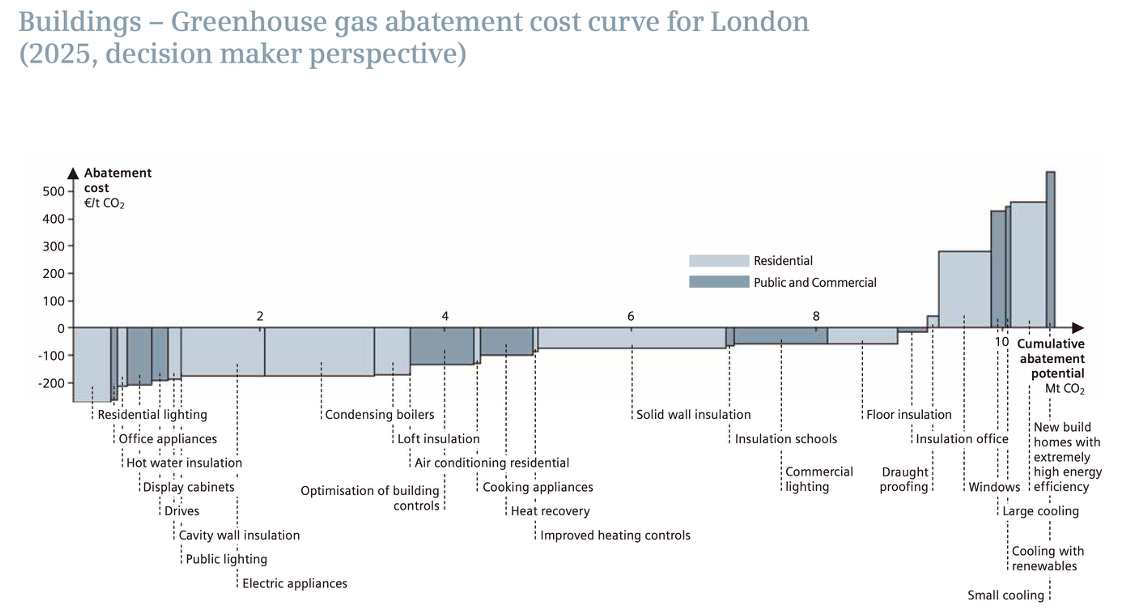
\includegraphics[width=0.99\linewidth]{Figures/building}
	\caption{Marginal Abatement Cost Curve (MACC) for the residential and commercial sectors. The vertical axis represents the cost to abate one tonne of CO$_2$, whilst the horizontal axis shows the cumulative reduction potential. Measures below the zero line—such as the \emph{optimisation of building controls}—offer a negative abatement cost, meaning they generate net financial savings over their lifetime. Source: Adapted from Siemens and McKinsey \& Company, \textit{\href{https://w3.siemens.com/topics/global/en/sustainable-cities/resilience/Documents/London_Final_Report_en.pdf}{Sustainable Urban Infrastructure: London Edition — A view to 2025}} (2008).}
	\label{fig:building}
\end{figure}

\subsection{Model Predictive Control for a One-Zone Building}

To illustrate how MPC can be applied in building energy management, this section
considers a simplified but representative example: a single thermal zone with
electrical heating and external disturbances from weather and solar radiation as shown in Figure~\ref{fig:singlezone}. Although simplified, the model captures the essential thermal dynamics and constraints that arise in real buildings, and it provides a clear foundation for constructing an MPC.

\begin{figure}
	\centering
	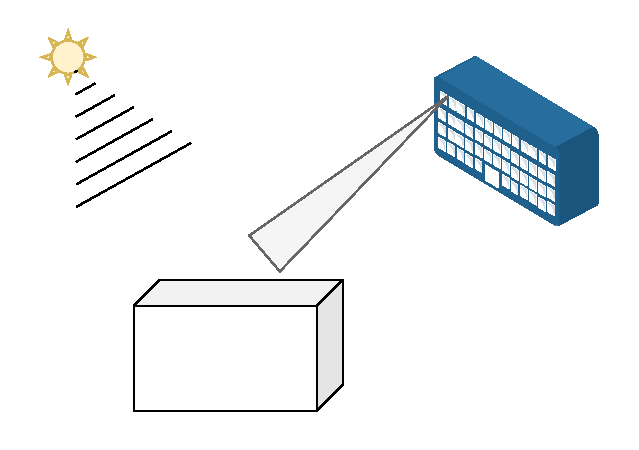
\includegraphics[width=0.7\linewidth]{Figures/SingleZone}
	\caption{Single zone of a building.}
	\label{fig:singlezone}
\end{figure}

The example is based on an EnergyPlus building model that has been
linearised and reduced automatically using the \emph{openBuild} tool.  
The resulting discrete-time state-space model has four states:
\[
x = \begin{bmatrix}
	x_1 \\ x_2 \\ x_3 \\ x_4
\end{bmatrix},
\qquad
x_1 = \text{zone air temperature}, \qquad
x_{2..4} = \text{wall temperatures}.
\]

The system evolves according to
\begin{equation}
	x_{k+1} = A x_k + B u_k
	+ E_{\mathrm{rad}}\, v^{\mathrm{rad}}_k
	+ E_{\mathrm{amb}}\, T^{\mathrm{amb}}_k,
	\label{eq:onezone_dynamics}
\end{equation}
where
\begin{itemize}
	\item \(u_k\) is the control input, representing the heat flux delivered to the zone,
	\item \(v^{\mathrm{rad}}_k\) is the incident solar radiation (a disturbance),
	\item \(T^{\mathrm{amb}}_k\) is the outdoor ambient temperature (another disturbance),
	\item \(A, B, E_{\mathrm{rad}}, E_{\mathrm{amb}}\) are obtained from linearisation.
\end{itemize}

The output of interest is the zone air temperature:
\[
y_k = c^\top x_k,
\]
where \(c^\top =\begin{bmatrix}
	1 & 0 & 0 & 0
\end{bmatrix}\) extracts the first state corresponding to \(x_1\).

\subsubsection{Control Objectives and Constraints}

The primary objective is to maintain the indoor temperature within a predefined
comfort band (e.g., around \(21^\circ\mathrm{C}\)) while minimising energy use.  
This naturally leads to the following requirements:
\begin{enumerate}
	\item \textbf{Comfort constraint}:
	\[
	|\,y_k - 21\,| \leq 2^\circ\mathrm{C}.
	\]
	\item \textbf{Actuator constraint} (electric heater):
	\[
	0 \leq u_k \leq 1,
	\]
	where \(u_k\) is normalised to the 0--100\% heating range.
	\item \textbf{Disturbance forecasts}:  
	Predictions of future weather (solar radiation and ambient temperature) 
	are incorporated over the MPC prediction horizon.  
	These forecasts are available from standard meteorological data.
\end{enumerate}

\subsubsection{MPC Problem Formulation}

The MPC problem aims to minimise energy use while satisfying comfort constraints.
Over a prediction horizon \(N\), the optimisation problem is:

\begin{equation}
	\begin{aligned}
		\min_{\{u_0,\dots,u_{N-1}\}} \quad &
		\sum_{i=0}^{N-1} |u_i|
		\\
		\text{s.t.} \quad &
		x_{i+1} = A x_i + B u_i + E_{\mathrm{rad}}\, v^{\mathrm{rad}}_i
		+ E_{\mathrm{amb}}\, T^{\mathrm{amb}}_i,
		\\
		& y_i = c^\top x_i,
		\\
		& |\,y_i - 21\,| \leq 2,
		\\
		& 0 \leq u_i \leq 1,
	\end{aligned}
	\label{eq:onezone_mpc}
\end{equation}

where:
\begin{itemize}
	\item The cost function \(\sum |u_i|\) represents total thermal energy consumption.
	\item The constraints enforce comfort and equipment limitations.
	\item Disturbance predictions enter the model explicitly through
	\(v^{\mathrm{rad}}_i\) and \(T^{\mathrm{amb}}_i\).
\end{itemize}

This formulation is intentionally simple and is the first step toward more advanced building MPC strategies. Later we shall extend this model to incorporate night-time temperature setbacks, pre-heating strategies, and time-of-use
 economic considerations while maintaining comfort. Figure~\ref{fig:building1} shows the application of the MPC and its evaluation. 


\begin{figure}
	\centering
	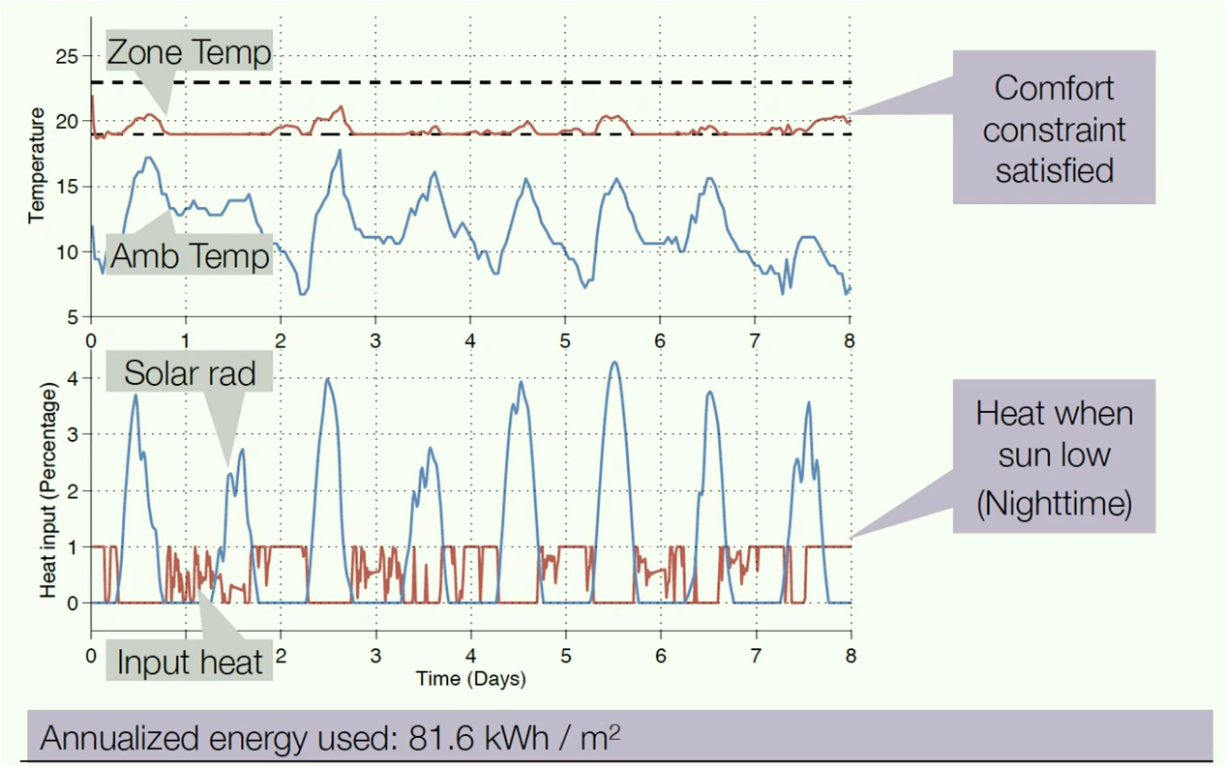
\includegraphics[width=0.95\linewidth]{Figures/building1}
	\caption{Closed-loop simulation results of Model Predictive Control (MPC) for a single-zone building. The top panel demonstrates the controller's ability to maintain the zone temperature (red line) within the specified comfort constraints (dashed lines), despite significant fluctuations in the ambient temperature (blue line). The bottom panel illustrates the relationship between the control input and disturbances; heating (red line) is applied primarily during nighttime or periods of low solar radiation (blue line) to compensate for heat loss, effectively minimizing energy use to an annualized rate of 81.6 kWh/m². (\textit{Taken from lecture slides of ME-425, EPFL with the permission of Prof C. Jones})}
	\label{fig:building1}
\end{figure}

\textbf{Can we do better with Model Predictive Control with Time-of-Use Pricing?}\\

In its simplest form, the controller's job is to minimise the total thermal energy consumed. But in modern smart grid setups, electricity prices change throughout the day depending on demand. To reflect this reality, we can shift the focus from minimising raw energy use to minimising the actual economic cost of running the system. We do this by incorporating a Time-of-Use tariff into the cost function.

\subsubsection{Problem Formulation}

We define a time-varying price vector $p \in \mathbb{R}^N$ over the prediction horizon. The tariff structure is defined based on peak and off-peak hours as follows:

\begin{equation*}
	p_k =
	\begin{cases}
		P_{\text{day}} & \text{if } 09:00 \le t_k < 18:00 \quad \text{(Peak)} \\
		P_{\text{night}} & \text{if } 18:00 \le t_k < 09:00 \quad \text{(Off-Peak)}
	\end{cases}
\end{equation*}

where $P_{\text{day}} > P_{\text{night}}$. The optimisation problem is now reformulated to minimise the weighted sum of the control inputs. Additionally, to ensure feasibility during aggressive load shifting, we introduce a slack variable $\sigma_i$ to relax the comfort constraints (soft constraints). If this is not done, the problem might become infeasible. The resulting optimisation problem can be written as:

\begin{align*}
	\min_{u, \sigma} \quad & \sum_{i=0}^{N-1} p_i |u_i| + \rho \|\sigma_i\| \\
	\text{s.t.} \quad & x_{i+1} = A x_i + B u_i + E_{\text{rad}} v_{i,\text{rad}} + E_{\text{amb}} T_{i,\text{amb}} \\
	& y_i = C x_i \\
	& |y_i - 21| \le 2 + \sigma_i \\
	& 0 \le u_i \le 1 \\
	& \sigma_i \ge 0
\end{align*}

where $\rho$ is a very large penalty weight to discourage comfort violations unless necessary. 

Introducing a price signal fundamentally changes how the controller behaves. Unlike the energy-optimal controller, which puts off heating until the very last moment, the economic-optimal controller uses the building's thermal mass as a kind of energy battery.

As Figure \ref{fig:tou_results} shows, the controller engages in load shifting and pre-heating. Knowing that prices will jump at 09:00, it heats the zone aggressively during the cheap off-peak hours in the early morning, pushing the temperature up towards the upper comfort limit of $23^\circ$. The thermal energy stored in the building's fabric then allows the system to dial back or switch off heating entirely during the expensive peak hours (09:00–18:00), keeping costs down whilst still maintaining occupant comfort.

\begin{figure}
	\centering
	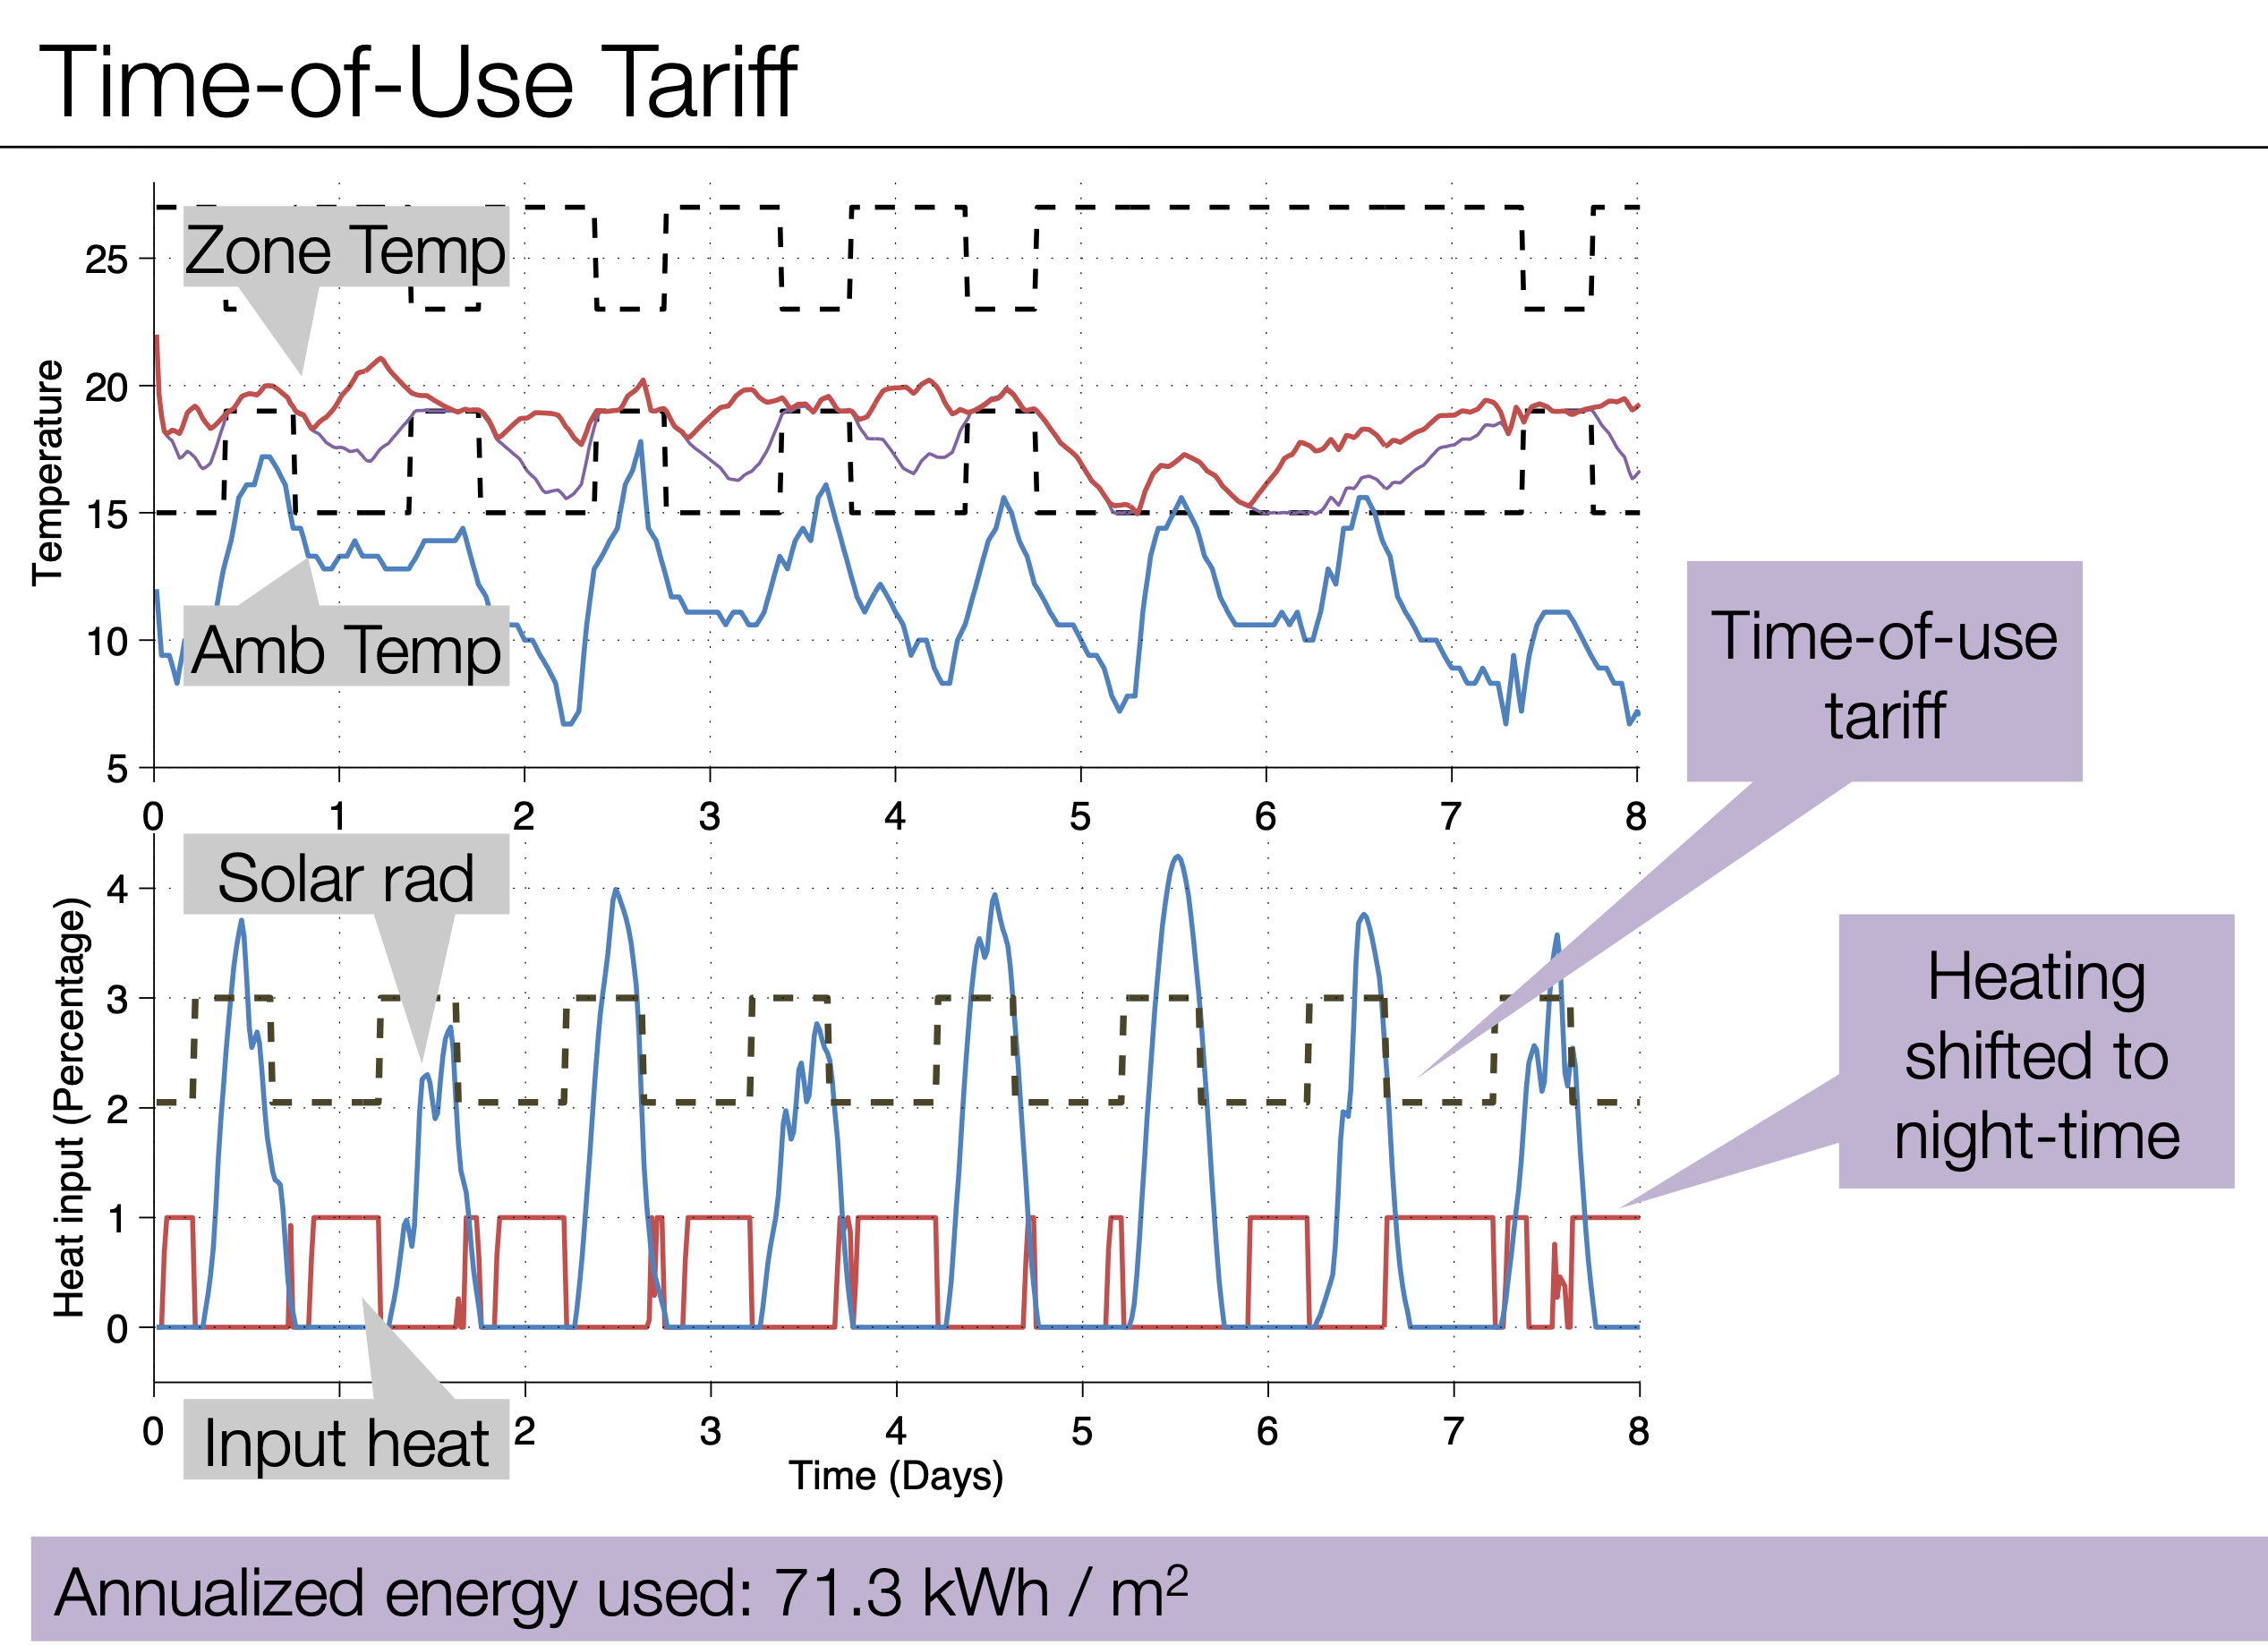
\includegraphics[width=0.95\linewidth]{Figures/building2}
	\caption{Simulation results under Time-of-Use (ToU) tariff. The bottom plot demonstrates the shifting of heating inputs to night-time hours to avoid high daytime electricity prices. (\textit{Taken from lecture slides of ME-425, EPFL with the permission of Prof C. Jones.})}
	\label{fig:tou_results}
\end{figure}


\section{A First MPC Example in MATLAB}

Before diving into the mathematical theory in the chapters that follow, it is instructive to see MPC in action on a simple example. The short MATLAB script below implements a complete MPC controller for a scalar unstable system using the YALMIP toolbox, so that the reader can run it immediately and build intuition for how the algorithm works.

\begin{lstlisting}[language=Matlab, caption={A minimal MPC example for a scalar unstable system.}, label={lst:first_mpc}]
	% 1. Define the scalar unstable system: x_{k+1} = 1.2*x_k + u_k
	A = 1.2;  B = 1;
	Q = 1;    R = 0.1;
	N = 10;   % Prediction horizon

	% Terminal cost from the discrete Riccati equation
	[P,~,~] = dare(A, B, Q, R);

	% 2. YALMIP formulation
	u = sdpvar(1, N);
	x = sdpvar(1, N+1);
	x0 = sdpvar(1, 1);        % Parameter: current state

	obj = 0;
	cons = [x(:,1) == x0];    % Initial condition constraint

	for k = 1:N
		obj  = obj + x(:,k)'*Q*x(:,k) + u(:,k)'*R*u(:,k);
		cons = [cons, x(:,k+1) == A*x(:,k) + B*u(:,k)];
		cons = [cons, -1 <= u(:,k) <= 1];   % Input constraint
	end
	obj = obj + x(:,N+1)'*P*x(:,N+1);       % Terminal cost

	% 3. Build the optimizer object (parametric in x0)
	opts = sdpsettings('verbose', 0, 'solver', 'quadprog');
	controller = optimizer(cons, obj, opts, x0, u(:,1));

	% 4. Closed-loop simulation
	T_sim = 30;
	x_state = 5;              % Initial condition
	x_hist = zeros(1, T_sim+1);  u_hist = zeros(1, T_sim);
	x_hist(1) = x_state;

	for t = 1:T_sim
		[u_opt, errcode] = controller(x_state);
		if errcode ~= 0, warning('Solver failed!'); end
		u_hist(t) = u_opt;
		x_state = A*x_state + B*u_opt;
		x_hist(t+1) = x_state;
	end

	% 5. Plot results
	figure;
	subplot(2,1,1);
	stairs(0:T_sim, x_hist, 'b', 'LineWidth', 2); grid on;
	ylabel('State (x)'); title('MPC Closed-Loop Response');
	subplot(2,1,2);
	stairs(0:T_sim-1, u_hist, 'b', 'LineWidth', 2); hold on;
	yline( 1, 'r--', 'LineWidth', 1.5);
	yline(-1, 'r--', 'LineWidth', 1.5);
	ylabel('Input (u)'); xlabel('Time step (k)'); grid on;
\end{lstlisting}

When you run this script, you should observe that the controller successfully drives the unstable state from $x_0 = 5$ to the origin despite the system being open-loop unstable ($a = 1.2$). Notice that the control input saturates at $u = -1$ during the first several time steps, when the state is large and the controller must apply maximum effort; once the state is sufficiently small, the input comes off the constraint and the controller smoothly regulates the state to zero.

\begin{notebox}{Prerequisites}
	This script requires MATLAB with the YALMIP toolbox and a QP solver such as \texttt{quadprog}. Installation instructions for YALMIP are given in the Foreword.
\end{notebox}


\section{Chapter Summary}

This chapter introduced Model Predictive Control (MPC) and contrasted it with classical control methods like PID. Unlike classical approaches that rely on pre-designed, fixed control laws, MPC solves a constrained optimisation problem on-line at each time step.

The main points are:

\begin{itemize}
	\item \textbf{Optimisation-Based Control:} MPC separates the \textit{control law} from the \textit{performance specifications}. Instead of tuning gains, the engineer defines a mathematical model of the plant, a cost function (objective), and physical constraints. The controller then solves an optimisation problem at every time step to find the best input sequence.
	
	\item \textbf{Receding Horizon Principle:} The operational backbone of MPC is the Receding Horizon Control (RHC) strategy. The controller measures the current state, plans a future trajectory over a finite horizon $N$, executes only the first step ($u_0$), and then repeats the process. This iterative re-planning provides the necessary feedback to handle uncertainties and disturbances, similar to a driver adjusting steering through a corner.
	
	\item \textbf{Explicit Constraint Handling:} A distinguishing feature of MPC is its ability to explicitly account for physical and safety limitations (e.g., valve limits, temperature bounds) during the design phase. While classical controllers clip signals when limits are reached, MPC anticipates these limits and steers the system along the constraint boundary to maximise performance safely.
	
	\item \textbf{Anticipation and Future Knowledge:} MPC is inherently predictive. It can utilise forecasts of known disturbances (such as weather or customer demand) to take pre-emptive action. 
	
	\item \textbf{Scalability:} The methodology is applicable across a vast range of time scales, from nanosecond-level processor control to week-level production planning, provided the optimisation problem can be solved within the sampling interval.
\end{itemize}

The chapter concluded with a practical application of MPC to a single-zone building, illustrating two distinct behaviours:
\begin{enumerate}
	\item \textbf{Energy Minimisation:} By incorporating weather forecasts, the MPC controller can reject disturbances (solar radiation, ambient temperature) efficiently, maintaining occupant comfort while minimising total energy use.
	\item \textbf{Economic Optimisation (Time-of-Use):} When electricity prices vary, MPC exploits the time-varying tariff structure. The controller exhibits \textit{load shifting} behaviours—specifically \textit{pre-heating}—where it overheats the building during off-peak hours (using the thermal mass as storage) to reduce expensive consumption during peak hours.
\end{enumerate}

MPC provides a systematic approach to controlling constrained, multivariable systems by formulating the control problem directly as a mathematical optimisation. For a comprehensive treatment of MPC theory and practice, the reader is referred to~\cite{Rawlings2017}.


\section*{Exercises}

\begin{enumerate}

	\item \textbf{The Receding Horizon Principle.}
	The receding horizon strategy is the operational backbone of MPC.
	\begin{enumerate}
		\item[(a)] In your own words, explain what ``receding horizon'' means. Why does the horizon ``recede'' at each time step?
		\item[(b)] At each time step, MPC computes an optimal sequence of $N$ future control inputs but only \emph{applies the first one} before solving the problem again. A student argues: ``This is wasteful—why not just apply the entire sequence and save computation?'' Write a short paragraph explaining why this approach would fail in practice. Your answer should mention at least two reasons (e.g., model mismatch, disturbances).
		\item[(c)] Consider the flowchart in Figure~\ref{fig:rhc_flowchart}. List, in order, the five steps the MPC controller performs at each sampling instant.
	\end{enumerate}

	\item \textbf{MPC versus PID and LQR.}
	Classical controllers such as PID and LQR are still widely used in industry.
	\begin{enumerate}
		\item[(a)] Give \emph{two} advantages that MPC has over a standard PID controller. For each advantage, briefly describe a real-world scenario where that advantage is critical.
		\item[(b)] Give \emph{one} practical disadvantage of MPC compared with PID. Under what circumstances would you recommend keeping a PID controller rather than replacing it with MPC?
		\item[(c)] The Linear Quadratic Regulator (LQR) also minimises a quadratic cost function of the form $\sum(x^\top Q x + u^\top R u)$. Identify \emph{one key difference} between LQR and MPC that explains why MPC is preferred when hard constraints on inputs or states must be satisfied.
		\item[(d)] Referring to the ``shower analogy'' in Section~1.4, describe in plain language how a \emph{decentralised PID} strategy and the \emph{MPC centralised} strategy each attempt to regulate both temperature and pressure. Why does the PID strategy lead to oscillation?
	\end{enumerate}

	\item \textbf{Numerical Exercise: Scalar System with Input Constraints.}
	Consider the scalar unstable system used in the MATLAB example (Listing~\ref{lst:first_mpc}):
	\[
		x_{k+1} = 1.2\, x_k + u_k,
	\]
	with initial state $x_0 = 5$ and input constraint $-1 \le u_k \le 1$.
	\begin{enumerate}
		\item[(a)] Without any controller ($u_k = 0$ for all $k$), compute the state values $x_1$, $x_2$, and $x_3$ starting from $x_0 = 5$. What does this tell you about the open-loop behaviour of the system?
		\item[(b)] Suppose the MPC controller applies the maximum allowed braking effort $u_k = -1$ at every step. Compute $x_1$, $x_2$, and $x_3$ under this saturated input. Is the system being stabilised? (\emph{Hint:} check whether $|x_k|$ is growing or shrinking.)
		\item[(c)] From the MATLAB description (Listing~\ref{lst:first_mpc} and the paragraph following it), the control input saturates at $u = -1$ during the first several time steps. Explain in one or two sentences \emph{why} the constraint is active at the start and why it eventually becomes inactive as the simulation progresses.
		\item[(d)] The cost function uses weights $Q = 1$ and $R = 0.1$. What does the choice $R < Q$ imply about the controller's priorities? What would change qualitatively if you set $R = 10$ instead?
	\end{enumerate}

	\item \textbf{Constraint Types: Hard vs.\ Soft, State vs.\ Input.}
	Constraints in MPC are categorised in two ways: by \emph{type} (hard or soft) and by \emph{variable} (state or input).
	\begin{enumerate}
		\item[(a)] \emph{Hard constraints} are constraints that must never be violated, while \emph{soft constraints} are relaxed by introducing a penalty term in the cost function. Give one example of a hard constraint and one example of a soft constraint in the building energy case study (Section~1.6). Explain why treating the comfort band as a soft constraint—rather than a hard one—can be important for ensuring the optimisation problem always has a solution.
		\item[(b)] In the building model, the actuator bound $0 \le u_k \le 1$ is an \emph{input constraint}, while the comfort requirement $|y_k - 21| \le 2$ is a \emph{state (output) constraint}. Explain, in plain language, the difference between these two types. Which type is typically easier to guarantee will always be satisfied, and why?
		\item[(c)] The Time-of-Use formulation in Section~1.6 introduces a slack variable $\sigma_i \ge 0$ that relaxes the comfort constraint to $|y_i - 21| \le 2 + \sigma_i$. Describe what happens to the comfort constraint if the penalty weight $\rho$ is set to a very large value versus a very small value.
		\item[(d)] Consider the vehicle example in Section~1.5 with state $x = [x_1, x_2]^\top$ (position, velocity) and acceleration input $u$. Write down, in words rather than matrices, one input constraint and one state constraint that would be physically reasonable for a road vehicle.
	\end{enumerate}

	\item \textbf{Building Energy Application: Forecast Errors and Controller Behaviour.}
	The building MPC case study relies on weather forecasts for outdoor temperature and solar radiation over the prediction horizon.
	\begin{enumerate}
		\item[(a)] Suppose the weather forecast predicts a mild day, but in reality a sudden cold snap arrives halfway through the day. Describe qualitatively what you would expect to happen to the indoor temperature under MPC. Would the situation be better or worse if the same forecast error occurred under a classical reactive (PID) controller? Justify your answer.
		\item[(b)] In the Time-of-Use strategy, the controller pre-heats the building during cheap off-peak hours in anticipation of expensive peak electricity prices (09:00--18:00). If the forecast for solar radiation is \emph{overestimated} (i.e., the controller expects more free solar heat than actually arrives), describe the likely consequence for occupant comfort during peak hours. Would you classify this as a failure of the model, the constraints, or the forecast?
		\item[(c)] The case study states that the annualised energy consumption is 81.6 kWh/m\textsuperscript{2}. Explain, in two or three sentences, how incorporating a Time-of-Use electricity tariff changes the \emph{pattern} of energy consumption even if the \emph{total} energy used over a day remains roughly the same.
		\item[(d)] MPC for buildings is listed as a ``negative abatement cost'' measure on the Marginal Abatement Cost Curve in Figure~\ref{fig:building}. In plain terms, what does this mean for a building owner? Why does smart control fall into this category whereas many other carbon-reduction measures do not?
	\end{enumerate}

\end{enumerate}




	% ===================================================================
% CHAPTER 2: OPTIMISATION
% ===================================================================

\chapter{Optimisation: The Engine of MPC}
\label{chap:optimisation}

\begin{quote}
	\textit{``Since the fabric of the universe is most perfect and the work of a most wise Creator, nothing at all takes place in the universe in which some rule of maximum or minimum does not appear.''} \\
	
	\hfill --- \textbf{Leonhard Euler}
\end{quote}


In Chapter~\ref{chap:introduction}, we introduced MPC as a controller that looks ahead and adjusts control actions by solving an optimisation problem at every time step. But this raises a fundamental question: how exactly does the computer decide which adjustment is the \emph{correct} one?

A classical PID controller follows a simple, fixed rule: if the error increases, push back harder. It is reactive and rigid. An MPC controller, however, does not follow a pre-written rule. Instead, at every single time step, it faces a choice. It determines the best control action within the given constraints. This process of systematic selection is called \emph{optimisation}.

Optimisation provides the mathematical framework for translating engineering objectives—such as \emph{drive fast but be safe}—into precise numerical instructions that a computer can understand. If the system model is the map that tells the controller where it \textit{can} go, optimisation is the navigator that decides where it \textit{should} go.

In this chapter, we step away from system dynamics for a moment to focus purely on this decision-making engine. We will learn how to formulate engineering goals as objective functions, how to translate physical limits into mathematical constraints, and how to distinguish between problems that are easy for computers to solve and those that are computationally impossible.

\section{What is Optimisation?}

In a general sense, the Oxford Dictionary defines optimisation as:
\begin{itemize}
	\item ``The action of making the \textbf{best} or \textbf{most effective} use of a situation or resource.''
\end{itemize}

In engineering, we translate this concept into a precise mathematical framework. We are not just ``trying to do our best''; we are systematically searching for a specific numerical value that satisfies a mathematical criterion.

\begin{defnbox}{Mathematical Definition of Optimisation}
	A numerical approach for seeking a \textbf{best} decision or action from a \textbf{set of alternatives}.
\end{defnbox}

\section{The Anatomy of an Optimisation Problem}

Formally, optimisation equates to the minimisation (or maximisation) of an \textit{objective function} $J(x)$, depending on a variable vector $x$, subject to constraints. The general mathematical problem is written as:

\begin{equation}
	\begin{aligned}
		\min_{x} \quad & J(x) \\
		\text{s.t.} \quad & x \in S
	\end{aligned}
\end{equation}

To translate a real-world engineering problem into the mathematical form described above, we must identify three fundamental components. Regardless of the complexity, almost every optimisation problem consists of:

\begin{enumerate}
	\item \textbf{Decision Variables ($x$):} These are the \emph{knobs} the solver can turn to minimise the cost. In the context of MPC, these variables usually represent the sequence of future control inputs (e.g., valve positions, motor currents, steering angles) over the prediction horizon.
	
	\item \textbf{Objective Function ($J$):} A scalar mathematical expression that quantifies \emph{performance}. The solver attempts to find the decision variables that result in the smallest possible value for this function. It typically represents physical quantities such as energy cost, tracking error, fuel consumption, or elapsed time.
	
	\item \textbf{Constraints:} The rules that must be obeyed. These define the \textit{feasible set} (denoted as $S$). Constraints distinguish practical engineering from pure mathematics by strictly enforcing physical limits (e.g., maximum voltage, tank capacity) or safety bounds (e.g., obstacle avoidance).
\end{enumerate}

Mathematically, we often denote the decision variables as $z$ to distinguish them from the system state $x$ used in control theory. The standard optimisation form is written as:

\begin{equation}
	\begin{aligned}
		\min_{x} \quad & J (x) \\
		\text{s.t.} \quad & g_i(x) \leq 0, \quad i=1,\ldots,m & \text{(Inequality constraints)} \\
		& h_j(x) = 0, \quad j=1,\ldots,q & \text{(Equality constraints)}
	\end{aligned}
\end{equation}

\begin{notebox}{Study note: Constraint Types}
	\begin{itemize}
	\item \textbf{Inequalities ($g \le 0$)} describe ranges, like ``speed must be less than 100 km/h''. \\
	\item \textbf{Equalities ($h = 0$)} describe strict physics, like $F = ma$. In MPC, the system dynamics ($x_{k+1} = Ax_k + Bu_k$) are treated as equality constraints. Note that here $x$ is the state of the system and not a decision variable. 
	\end{itemize}
\end{notebox}

\section{Illustrative Examples}

To make the abstract definitions of decision variables, objective functions, and constraints concrete, let us consider two distinct optimisation problems.

The process of translating a physical or data-driven problem into a mathematical optimisation format is known as \textbf{modelling}. This step is often more challenging than the solution itself. In both examples below, we follow a systematic three-step approach:
\begin{enumerate}
	\item \textbf{Identify the Decision Variables:} What are the \emph{knobs} we can turn?
	\item \textbf{Formulate the Objective:} What is the single metric that defines \emph{best}?
	\item \textbf{Define the Constraints:} What are the physical or logical limits we must obey?
\end{enumerate}

The first example (Box Volume) illustrates a geometric design problem where \emph{physical constraints} play a critical role—analogous to actuator limits in control systems. The second example (Linear Regression) introduces the concept of \emph{least-squares minimisation}, which is the mathematical foundation for data science.

\begin{examplebox}{Maximising Box Volume}
	\textbf{Problem Statement:} Given a square piece of cardboard with dimensions $1\,\text{m} \times 1\,\text{m}$ as shown in Figure~\ref{fig:box_volume}, we wish to construct an open-top box with the maximum possible volume. We achieve this by cutting equal squares of side length $x$ from the four corners and folding up the sides.
	

	\begin{center}
		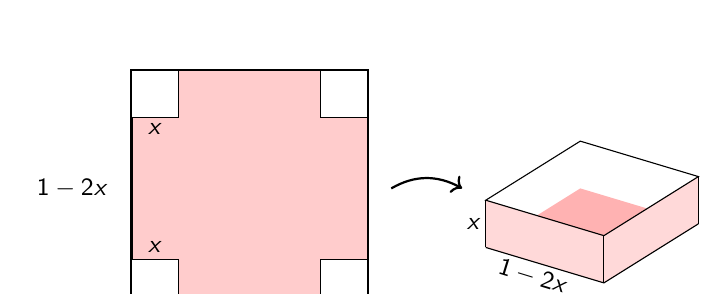
\begin{tikzpicture}[scale=1.5]
			% SMALLER VERSION OF THE FIGURE FOR INSIDE THE BOX
			% 2D Sheet
			\fill[red!20] (0,0) rectangle (2,2);
			\draw[thick] (0,0) rectangle (2,2);
			\foreach \x/\y in {0/0, 1.6/0, 0/1.6, 1.6/1.6} {
				\fill[white, draw=black] (\x,\y) rectangle (\x+0.4,\y+0.4);
			}
			\node at (0.2, 1.5) {\small $x$};
			\node at (-0.5, 1) {\small $1-2x$};
			\node at (0.2, 0.5) {\small $x$};
			
			% Arrow
			\draw[->, thick, bend left] (2.2, 1) to (2.8, 1);
			
			% 3D Box
			\begin{scope}[xshift=3cm, yshift=0.5cm]
				\coordinate (A) at (0,0);
				\node at (-0.1, 0.2) {\small $x$};
				\coordinate (B) at (1.0, -0.3); 
				\coordinate (C) at (1.8, 0.2); 
				\coordinate (Ah) at (0, 0.4);
				\coordinate (Bh) at (1.0, 0.1);
				\coordinate (Ch) at (1.8, 0.6);
				\coordinate (Dh) at (0.8, 0.9);
				\fill[red!30] (A) -- (B) -- (C) -- (0.8,0.5) -- cycle;
				\fill[red!15] (A) -- (B) -- (Bh) -- (Ah) -- cycle;
				\fill[red!15] (B) -- (C) -- (Ch) -- (Bh) -- cycle;
				\draw (A) -- (B) -- (C);
				\draw (Ah) -- (Bh) -- (Ch) -- (Dh) -- cycle;
				\draw (A) -- (Ah); \draw (B) -- (Bh); \draw (C) -- (Ch);
				\node[rotate=-17] at (0.4, -0.25) {\small $1-2x$};
			\end{scope}
		\end{tikzpicture}
	\end{center}
	\captionof{figure}{Box volume maximisation problem.}
	\label{fig:box_volume}
	\solution
	
	We map this problem to the three components of optimisation:
	
	\begin{enumerate}
		\item \textbf{Decision Variable ($x$):} The size of the corner cut.
		\item \textbf{Constraints:} 
		\begin{itemize}
			\item The cut must be positive: $x \geq 0$.
			\item The cut cannot overlap (total width is 1m): $2x \leq 1 \implies x \leq 0.5$.
		\end{itemize}
		\item \textbf{Objective Function:} Maximise Volume $V = \text{length} \times \text{width} \times \text{height}$.
		\[ J(x) = \underbrace{(1-2x) \cdot (1-2x)}_{\textbf{Base Area}} \cdot x = x(1-2x)^2 \]
	\end{enumerate}
	
	\textbf{Mathematical Formulation:}\footnote{ \textbf{Note on Standard Form:} While this example seeks to \textit{maximise} volume, most standard solvers (including \texttt{quadprog} in MATLAB) are designed to \textit{minimise} functions. In engineering practice, we simply flip the sign of the objective function. Maximising $f(x)$ is mathematically equivalent to minimising $-f(x)$.}
	\begin{equation*}
		\begin{aligned}
			\max_{x} \quad & x(1-2x)^2 \\
			\text{s.t.} \quad & 0 \leq x \leq 0.5
		\end{aligned}
	\end{equation*}
	or equivalently
		\begin{equation*}
		\begin{aligned}
			\min \quad & -x(1-2x)^2 \\
			\text{s.t.} \quad & 0 \leq x \leq 0.5
		\end{aligned}
		\end{equation*}
\end{examplebox}


\begin{examplebox}{Linear Regression (Least Squares)}
	\textbf{Problem Statement:} Suppose we are given a dataset containing $N$ pairs of experimental measurements: $\{(x_1, y_1), (x_2, y_2), \dots, (x_N, y_N)\}$ as shown in Figure~\ref{fig:linear_regression}.
	
	We want to find the linear model (a straight line) that "best fits" this data.
	
	\begin{center}
		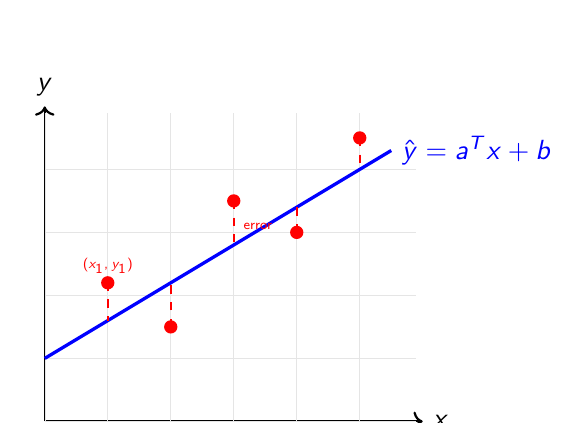
\begin{tikzpicture}[scale=0.8]
			% Axes
			\draw[->, thick] (0,0) -- (6,0) node[right] {$x$};
			\draw[->, thick] (0,0) -- (0,5) node[above] {$y$};
			\draw[step=1cm, gray!20, very thin] (0,0) grid (5.9,4.9);
			
			% The Model Line
			\draw[blue, very thick] (0,1) -- (5.5, 4.3) node[right] {$\hat{y} = a^T x + b$};
			
			% Data Points
			\foreach \p/\x/\y in {1/1/2.2, 2/2/1.5, 3/3/3.5, 4/4/3.0, 5/5/4.5} {
				\draw[dashed, red, thick] (\x, \y) -- (\x, {0.6*\x + 1}); % Residual
				\fill[red] (\x, \y) circle (3pt);
			}
			% Labels
			\node[red, above] at (1, 2.2) {\tiny $(x_1, y_1)$};
			\node[right, red] at (3, 3.1) {\tiny error};
		\end{tikzpicture}
		\captionof{figure}{Dataset (red), linear interpolation (blue).}
		\label{fig:linear_regression}
	\end{center}
	
	\solution
	
	Note that in this specific problem, the $x$ values are \textbf{constants} (data we measured), not decision variables.
	
	\begin{enumerate}
		\item \textbf{Decision Variables:}  The parameters of the line: the slope vector $a \in \mathbb{R}^n$ and the intercept $b \in \mathbb{R}$.
		\begin{itemize}
			\item Note: In the 2D plot above, $n=1$, so $a$ is a scalar slope. However, the math holds for $n$-dimensional vectors.
		\end{itemize}
		
		\item \textbf{Objective Function:} We define the prediction for the $i$-th data point as $\hat{y}_i = a^T x_i + b$. We want to minimise the Sum of Squared Errors (SSE):
		\[ J(a, b) = \sum_{i=1}^{N} (y_i - \hat{y}_i)^2 = \sum_{i=1}^{N} \left( y_i - (a^T x_i + b) \right)^2 \]
		
		\item \textbf{Constraints:} In this case, $a$ and $b$ can be any real numbers. There are no restrictions. Therefore this is an unconstrained optimisation. 
	\end{enumerate}
	
	\textbf{Mathematical Formulation:}\\
	
	\begin{equation*}
		\min_{a, b} \quad \sum_{i=1}^{N} \left( y_i - (a^T x_i + b) \right)^2 
	\end{equation*}
\end{examplebox}


\section{Ingredients of Multi-Variable Optimisation}

In the previous examples (the box and the line fitting), we dealt with specific cases. Now, let us formalise the general structure of an optimisation problem involving multiple variables. This is the exact structure used in Model Predictive Control, where we must simultaneously optimise a sequence of inputs over time.

\subsection{Problem Setting: The Decision Vector}

In real-world engineering, we rarely make a single scalar decision. Instead, we must determine a set of $n$ values simultaneously. To handle this mathematically, we collect all individual decision variables ($x_1, x_2, \dots, x_n$) into a single \emph{decision vector}: $x \in \mathbb{R}^n$:
\begin{equation}
	x = \begin{bmatrix} x_1 \\ x_2 \\ \vdots \\ x_n \end{bmatrix}
\end{equation}
Then the objective function $J$ maps this vector to a scalar real number (a score or cost):
\[ J: \mathbb{R}^n \to \mathbb{R} \]
For example, in MPC, if we have a control horizon of 10 steps and 2 inputs, our decision vector $x$ has a dimension of $n=20$.

\subsection{Understanding Vector-to-Scalar Mapping: The \emph{cost} function}

The mathematical notation $J: \mathbb{R}^n \to \mathbb{R}$ often confuses beginners. It reads: \textit{"The function $f$ takes a vector of $n$ numbers and transforms it into a single real number."}

To understand why this is necessary, let us consider a relatable real-world analogy: The Shopping Basket.

\subsubsection*{The Analogy}

Imagine you are at a supermarket checkout.

\begin{enumerate}
	\item \textbf{The Vector ($x$):} Your shopping basket contains many different items. You might have 2 loaves of bread, 6 eggs, and 1 litre of milk. We can list these quantities as a vector:
	\[ 
	x = \begin{bmatrix} 2 \\ 6 \\ 1 \end{bmatrix} 
	\begin{matrix} \leftarrow \text{Bread} \\ \leftarrow \text{Eggs} \\ \leftarrow \text{Milk} \end{matrix}
	\]
	This vector represents the \textit{state} of your shopping. It is multi-dimensional because it contains different types of information.
	
	\item \textbf{The Objective Function ($J$):} The checkout till scans your items. It applies a specific rule (the price list) to your vector. It multiplies each item by its value and sums them up:
	\[ 
	J(x) = (2 \times \pounds 1.00) + (6 \times \pounds 0.20) + (1 \times \pounds 0.80) 
	\]
	
	\item \textbf{The Scalar ($J$):} The till produces a single number: {\pounds 4.00}.
\end{enumerate}
This is visually described in Figure~\ref{fig:cost_function_analogy}. 
\begin{center}
	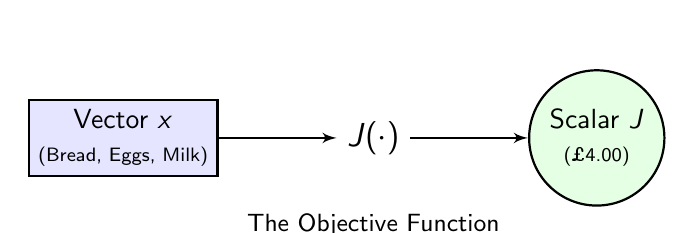
\begin{tikzpicture}[node distance=2cm, auto, >=latex', thick]
		% Nodes
		\node [draw, rectangle, align=center, fill=blue!10, minimum height=2.5em] (vector) {Vector $x$\\ \scriptsize (Bread, Eggs, Milk)};
		\node [right=1.5cm of vector] (func) {\large $J(\cdot)$};
		\node [draw, circle, align=center, fill=green!10, right=1.5cm of func, minimum size=2.5em] (scalar) {Scalar $J$\\ \scriptsize (\pounds 4.00)};
		
		% Arrows
		\draw [->] (vector) -- (func);
		\draw [->] (func) -- (scalar);
		
		% Label
		\node [below=0.5cm of func] {\small The Objective Function};
	\end{tikzpicture}
	\captionof{figure}{Analogy of cost function.}
	\label{fig:cost_function_analogy}
\end{center}

\subsubsection*{Why is this important in Engineering?}

You cannot easily say which of two shopping baskets is \emph{larger} just by looking at the items—one might have more eggs but no milk. However, once you map them to a {scalar} (the total price), comparison becomes easy. You can instantly say which basket costs less.

In Model Predictive Control, our \emph{basket} ($x$) contains complex decisions: valve positions, heater settings, and motor speeds over the next 20 minutes. We cannot simply look at two different plans and say \emph{Plan A is better than Plan B,} because Plan A might use less fuel but Plan B might track the temperature better.

The objective function $J(x)$ squashes all these complex, multi-dimensional decisions into a single number (a score). 
\begin{itemize}
	\item If Plan A scores $10.5$ and Plan B scores $8.2$, and we are minimising cost, we know for a fact that {Plan B is the mathematical winner}.
\end{itemize}

\begin{notebox}{Key Takeaway}
	Optimisation algorithms cannot minimise a list or a vector. They can only minimise a single number. The objective function acts as a \emph{translator}, converting a complex list of engineering decisions into a single score that allows us to rank them.
\end{notebox}

\subsection{Constraints and the Feasible Set}


We rarely operate in an ideal world. Our decisions are restricted by physical limits. These restrictions are defined by a finite number of equations or inequalities involving the decision variables.

\begin{enumerate}
	\item \textbf{Inequality Constraints ($g_i$):} These represent bounds, such as "Temperature must be less than $100^{\circ}\mathrm{C}$" or "Valve must be open at least 10\%".
	\[ g_i(x) \leq b_i, \quad i = 1, \dots, m \]
	
	\item \textbf{Equality Constraints ($h_j$):} These represent strict physics or model dynamics, such as \emph{Input flow must equal output flow} or $F = ma$.
	\[ h_j(x) = 0, \quad j = 1, \dots, q \]
	
	\item \textbf{Domain Restrictions:} Sometimes variables are not continuous. For instance, a switch is either ON (1) or OFF (0). If $p$ variables are discrete (integers) and the rest are continuous, we denote the domain as $x \in \mathbb{R}^{n-p} \times \mathbb{Z}^p$. Note that dealing with domain restrictions is difficult in optimisation. 
\end{enumerate}


Collectively, these constraints define a specific region in the $n$-dimensional space called the \emph{Feasible Set} $S$. The optimisation algorithm is only allowed to search for solutions within this set.
\begin{equation}
	S = \{ x \in \mathbb{R}^n \mid g_i(x) \leq b_i \ \forall i, \ h_j(x) = 0 \ \forall j \}
\end{equation}
If the intersection of these constraints is empty (e.g., $x > 5$ AND $x < 3$), the problem is \textit{infeasible}—there is no solution.

\begin{examplebox}{Visualising the Feasible Set}
	Consider a 2-dimensional problem ($x \in \mathbb{R}^2$) with two inequality constraints:
	\begin{enumerate}
		\item $g_1(x) = x_1^2 + x_2^2 \leq 4$ (Must be inside a circle of radius 2).
		\item $g_2(x) = x_1^3 - x_2 \leq 0 \implies x_2 \geq x_1^3$ (Must be above the cubic curve).
	\end{enumerate}
	The feasible set $S$ is the intersection of these two regions (the purple area as shown in Figure~\ref{fig:intersection_of_constraints}).
	
	\begin{center}
		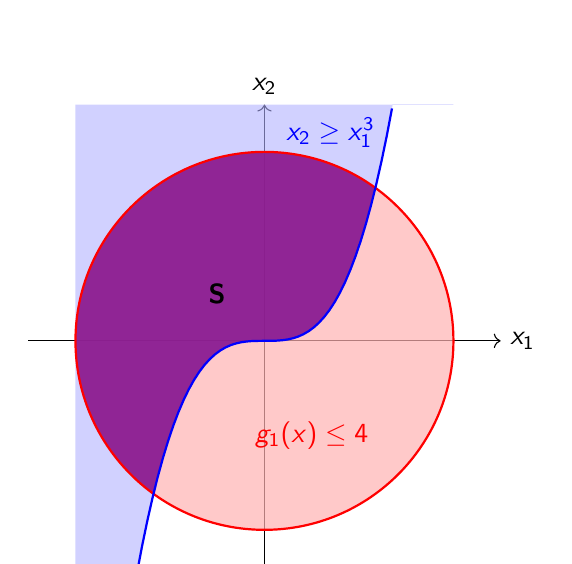
\begin{tikzpicture}[scale=1.2]
			% Draw Axes
			\draw[->] (-2.5,0) -- (2.5,0) node[right] {$x_1$};
			\draw[->] (0,-2.5) -- (0,2.5) node[above] {$x_2$};
			
			% Region 1: Circle x^2 + y^2 <= 4 (Red)
			% We fill with opacity
			\fill[red!30, opacity=0.7] (0,0) circle (2cm);
			
			% Region 2: x2 >= x1^3 (Blue)
			% We clip a rectangle to the area above the curve
			\begin{scope}
				\clip (-2.5, -2.5) rectangle (2.5, 2.5);
				\fill[blue!30, opacity=0.6] plot[domain=-2:2, samples=50] (\x, {\x*\x*\x}) |- (-2,2.5) -- cycle;
			\end{scope}
			
			% Re-draw Intersection (Purple/Darker) to emphasize
			\begin{scope}
				\clip (0,0) circle (2cm);
				\fill[blue!50!red, opacity=0.8] plot[domain=-1.3:1.3, samples=50] (\x, {\x*\x*\x}) |- (-2,2.5) -- (-2, -2.5) -- cycle;
			\end{scope}
			
			% Draw Boundaries
			\draw[thick, red] (0,0) circle (2cm);
			\node[red] at (.5, -1.) {$g_1(x) \le 4$};
			
			\draw[thick, blue, domain=-1.35:1.35, samples=50] plot (\x, {\x*\x*\x});
			\node[blue] at (0.7, 2.2) {$x_2 \ge x_1^3$};
			
			\node at (-0.5, 0.5) {\textbf{S}};
		\end{tikzpicture}
		\captionof{figure}{Intersection of constraints. Blue region $x_2 \ge x_1^3$, red region $x_1^2+x_2^2 \le 4$. $S$ is the intersection and the feasible domain.}
		\label{fig:intersection_of_constraints}
	\end{center}
\end{examplebox}

\subsection{Standard Form: Minimisation vs. Maximisation}

Standard numerical solvers (like \texttt{quadprog} or \texttt{fmincon} in MATLAB) are typically written to perform \textbf{minimisation}. However, engineering problems are often phrased as maximisation (e.g., maximise profit, maximise volume).

To reconcile this, we rely on a mathematical identity. But first, we must clarify a precise piece of notation often used in optimisation: the difference between $\min$ and $\arg \min$.

\textbf{Notation Note: Minimum vs. Argument of the Minimum:} \\

\begin{itemize}
	\item \textbf{$\min f(x)$:} Returns the \textbf{value} of the function at the minimum. This is the score (the vertical axis on a graph).
	\item \textbf{$\arg \min f(x)$:} Returns the {argument} (the variable $x$) that produces that minimum. This is the decision (the horizontal axis).
\end{itemize}

In MPC, we are primarily interested in the $\arg \min$ because we need to know \textit{what input $u$ to apply} to the system, not just what the theoretical cost is.

\textbf{Converting Maximisation to Minimisation:}\\

With this notation in mind, we can state the equivalence principle. We do not need separate software to solve maximisation problems. We rely on the identity that finding the argument that maximises a function is equivalent to finding the argument that minimises its negative:

\begin{equation}
	\underbrace{\arg \max_{x \in S} f(x)}_{\text{Best Decision}} \equiv \underbrace{\arg \min_{x \in S} \{-f(x)\}}_{\text{Equivalent Search}}
\end{equation}

Visually, multiplying the objective function by $-1$ flips the curve upside down. A peak (maximum) in the original function becomes a valley (minimum) in the negated function. While the vertical values flip signs, the \textbf{horizontal location ($x$)} of the optimal point remains exactly the same. This is pictured in Figure~\ref{fig:minimization_vs_max}.

\begin{figure}
	\begin{center}
		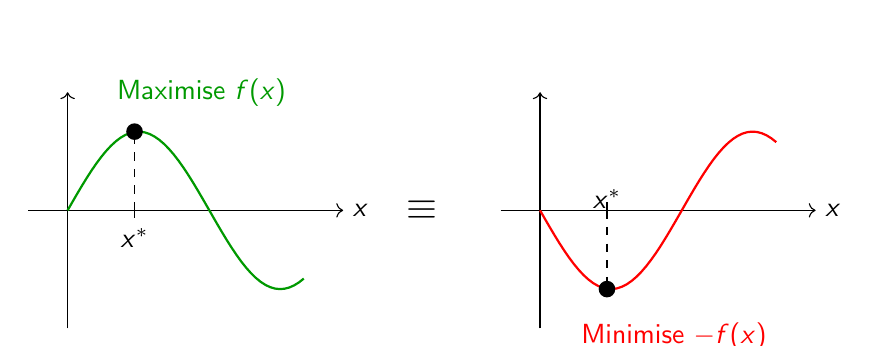
\begin{tikzpicture}[scale=1]
			% Maximisation Plot
			\begin{scope}
				\draw[->] (-0.5,0) -- (3.5,0) node[right] {$x$};
				\draw[->] (0,-1.5) -- (0,1.5);
				
				% Draw the function
				\draw[thick, green!60!black] plot[domain=0:3, samples=50] (\x, {sin(\x*100)});
				\node[green!60!black] at (1.7, 1.5) {Maximise $f(x)$};
				
				% Draw x* lines and labels
				\draw[dashed] (0.85, 0) -- (0.85, 1);
				\draw (0.85, 0.1) -- (0.85, -0.1) node[below] {$x^*$}; % Tick mark and label
				
				% Draw the optimal point
				\fill[black] (0.85, 1) circle (3pt);
			\end{scope}
			
			% Equivalence Symbol
			\node at (4.5, 0) {\Large $\equiv$};
			
			% Minimisation Plot
			\begin{scope}[xshift=6cm]
				\draw[->] (-0.5,0) -- (3.5,0) node[right] {$x$};
				\draw[->] (0,-1.5) -- (0,1.5);
				
				% Draw the function
				\draw[thick, red] plot[domain=0:3, samples=50] (\x, {-sin(\x*100)});
				\node[red] at (1.7, -1.6) {Minimise $-f(x)$};
				
				% Draw x* lines and labels
				\draw[dashed] (0.85, 0) -- (0.85, -1);
				\draw (0.85, 0.1) -- (0.85, -0.1) node[above] {$x^*$}; % Tick mark and label
				
				% Draw the optimal point
				\fill[black] (0.85, -1) circle (3pt);
			\end{scope}
		\end{tikzpicture}
	\end{center}
	\caption{Visual representation of the equivalence between maximisation and minimisation. To maximise an objective function $f(x)$ (green curve), one can equivalently minimise its negative, $-f(x)$ (red curve). Note that while the vertical value flips sign, the optimal decision variable $x^*$ (the horizontal position of the black dot) remains identical.}
	\label{fig:minimization_vs_max}
\end{figure}

Therefore, in this course, we will consistently formulate our MPC problems as minimisation tasks, usually minimising an energy or error cost function.



% ===================================================================
% SECTION: CLASSIFICATION OF PROBLEMS
% ===================================================================

\section{Terminology in Optimisation}

With the general structure of an optimisation problem in place, we now refine the vocabulary. Some optimisation problems can be solved in milliseconds on a cheap microcontroller, whilst others might take days on a supercomputer and still fail to find the best solution.

The distinguishing factor is rarely just the size of the problem (the number of variables); rather, it is the geometry of the problem.

The difference between easy and hard problems lies not in the number of variables but in the geometry of the search space. The central concept here is \textbf{Convexity}: if the objective is convex and the constraints form a convex set, then any local minimum is guaranteed to be the global minimum. We begin by defining the building blocks of this geometry: sets and functions.

\subsection{Convex Sets}

A fundamental concept in optimisation, particularly in Model Predictive Control (MPC), is that of a \textbf{convex set}. Working with convex sets and functions simplifies the optimisation problem significantly, often guaranteeing that any local optimum is also a global optimum.

\begin{defnbox}{Convex Set}
	A set $\mathcal{X}$ is \textbf{convex} if and only if for any pair of points $x$ and $y$ in $\mathcal{X}$, any \textbf{convex combination} of $x$ and $y$ lies in $\mathcal{X}$.
\end{defnbox}

Mathematically, this definition is stated as:
$$
\mathcal{X} \text{ is convex} \quad \Longleftrightarrow \quad \lambda x + (1 - \lambda)y \in \mathcal{X}, \quad \forall \lambda \in [0, 1], \quad \forall x, y \in \mathcal{X}
$$
The term $\lambda x + (1 - \lambda)y$ represents a line segment connecting $x$ and $y$.

\begin{notebox}{Interpretation}
	All line segments starting and ending in $\mathcal{X}$ stay within $\mathcal{X}$.
\end{notebox}


To illustrate the concept, consider the following examples of convex and non-convex sets.

\begin{figure}[h!]
	\centering
	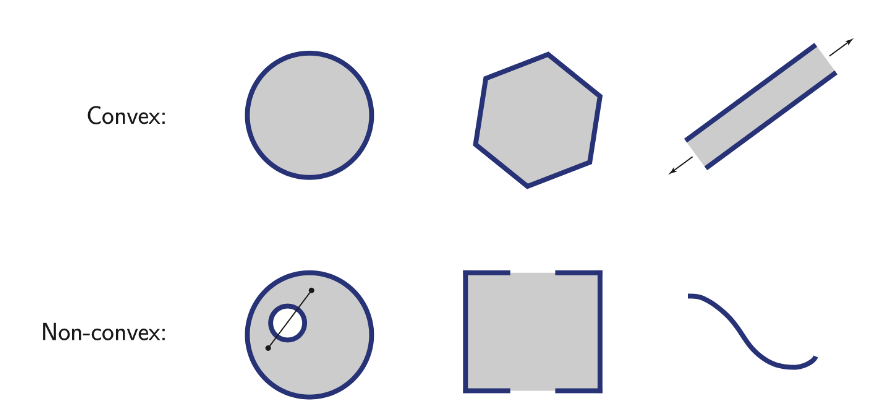
\includegraphics[width=0.7\textwidth]{Figures/convex_sets}
	\caption{Visual examples of convex and non-convex sets. A set is non-convex if a line segment connecting two of its points leaves the set.}
	\label{fig:convexsets}
\end{figure}

In the context of Model Predictive Control (MPC), constraints are often defined by linear inequalities. Geometrically, these constraints represent hyperplanes and half-spaces. Understanding these geometric primitives is essential because they form the building blocks of convex sets.


\begin{defnbox}{Hyperplane}
A hyperplane is a set of the form:
\begin{equation}
	\{x \in \mathbb{R}^n \mid a^\top x = b\}
\end{equation}
where $a \in \mathbb{R}^n$ (with $a \neq 0$) and $b \in \mathbb{R}$. The vector $a$ is the \textit{normal vector} to the hyperplane; it is orthogonal to any vector lying within the hyperplane.

In $\mathbb{R}^2$, a hyperplane defines a line. In $\mathbb{R}^3$, it defines a plane. This is shown on the left of Figure~\ref{fig:hyperplane_halfspace}.
\end{defnbox}

\begin{defnbox}{Half space}
	A hyperplane divides the space $\mathbb{R}^n$ into two halves. A half-space is the set of points on one side of (or on) the hyperplane:
\begin{equation}
	\{x \in \mathbb{R}^n \mid a^\top x \leq b\}
\end{equation}
This is known as a \textit{closed} half-space because it includes the boundary (the hyperplane itself). If the inequality is strict ($<$), it is an \textit{open} half-space. This is shown on the right of Figure~\ref{fig:hyperplane_halfspace}.
\end{defnbox}

Hyperplanes and half-spaces are always convex sets. This property ensures that optimisation problems with linear constraints remain convex.

\begin{figure}[!h]
	\centering
	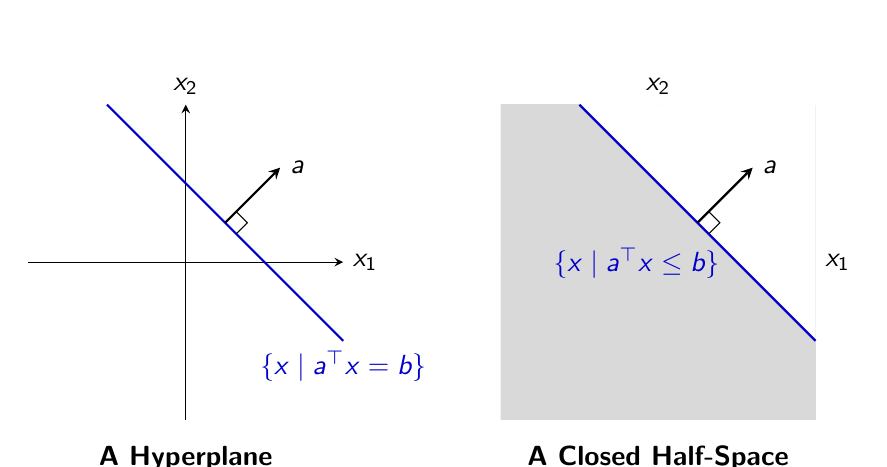
\begin{tikzpicture}[scale=1, >=stealth]
		% LEFT PLOT: Hyperplane
		\begin{scope}
			\draw[->] (-2,0) -- (2,0) node[right] {$x_1$};
			\draw[->] (0,-2) -- (0,2) node[above] {$x_2$};
			
			% Line: x1 + x2 = 1 => x2 = -x1 + 1
			\draw[thick, blue!80!black] (-1, 2) -- (2, -1) node[below] {$\{x \mid a^\top x = b\}$};
			
			% Normal vector a = (1,1). Placed at (0.5, 0.5)
			\draw[->, thick] (0.5, 0.5) -- (1.2, 1.2) node[right] {$a$};
			
			% Right angle symbol
			\draw[rotate around={-45:(0.5,0.5)}] (0.5, 0.7) -- (0.7, 0.7) -- (0.7, 0.5);
			
			\node at (0, -2.5) {\textbf{A Hyperplane}};
		\end{scope}
		
		% RIGHT PLOT: Half-space
		\begin{scope}[xshift=6cm]
			\draw[->] (-2,0) -- (2,0) node[right] {$x_1$};
			\draw[->] (0,-2) -- (0,2) node[above] {$x_2$};
			
			% Fill the area x1 + x2 <= 1
			\fill[gray!30] (-2, -2) rectangle (2, 2);
			\fill[white] (-1, 2) -- (2, -1) -- (2, 2) -- (-1, 2); 
			% (Alternative simple clip for halfspace)
			\begin{scope}
				\clip (-2,-2) rectangle (2,2);
				\fill[gray!30] (-3, 4) -- (4, -3) -- (-3, -3) -- cycle;
			\end{scope}
			
			% Line
			\draw[thick, blue!80!black] (-1, 2) -- (2, -1);
			\node[blue!80!black, below left] at (0.9, 0.3) {$\{x \mid a^\top x \leq b\}$};
			
			% Normal vector
			\draw[->, thick] (0.5, 0.5) -- (1.2, 1.2) node[right] {$a$};
			
			% Right angle symbol
			\draw[rotate around={-45:(0.5,0.5)}] (0.5, 0.7) -- (0.7, 0.7) -- (0.7, 0.5);
			
			\node at (0, -2.5) {\textbf{A Closed Half-Space}};
		\end{scope}
	\end{tikzpicture}
	\caption{Visual representation of a hyperplane (left) and a closed half-space (right). The vector $a$ is normal to the boundary.}
	\label{fig:hyperplane_halfspace}
\end{figure}

\begin{examplebox}{Linear Constraint in $\mathbb{R}^2$}
	
	Consider a linear relation defined by the equation:
	\begin{equation}
		2x_1 + 1x_2 = 2
	\end{equation}
	This represents a line in 2D space. To relate this to the standard hyperplane definition $a^\top x = b$, we define the vectors:
	\begin{equation}
		a = \begin{pmatrix} 2 \\ 1 \end{pmatrix}, \quad x = \begin{pmatrix} x_1 \\ x_2 \end{pmatrix}, \quad b = 2
	\end{equation}
	Thus, the equation becomes:
	\begin{equation}
		\underbrace{\begin{pmatrix} 2 & 1 \end{pmatrix}}_{a^\top} \begin{pmatrix} x_1 \\ x_2 \end{pmatrix} = \underbrace{2}_{b}
	\end{equation}
	
	\textbf{Connection to the Gradient:}\\

	Readers needing a refresher on vectors, matrices, and eigenvalues may consult Appendix~\ref{app:linalg}.

	We can also view this through the lens of multivariate calculus. Let us define a function $f(x)$ implicitly by the zero-level set:
	\begin{equation}
		f(x) = 2x_1 + x_2 - 2 = 0
	\end{equation}
	The gradient of this function, denoted as $\nabla f$, is a column vector containing the partial derivatives with respect to $x_1$ and $x_2$:
	\begin{equation}
		a = \nabla_x f = \begin{pmatrix} \dfrac{\partial f}{\partial x_1} \\[12pt] \dfrac{\partial f}{\partial x_2} \end{pmatrix} = \begin{pmatrix} 2 \\ 1 \end{pmatrix}
	\end{equation}
	This confirms that the vector $a = (2, 1)^\top$ is the gradient of the linear function defining the hyperplane. Geometrically, the gradient vector is perpendicular to the level sets of the function, meaning $a$ is perpendicular to the line $2x_1 + x_2 = 2$, as shown in Figure \ref{fig:example_hyperplane}.
	
		\begin{center}
		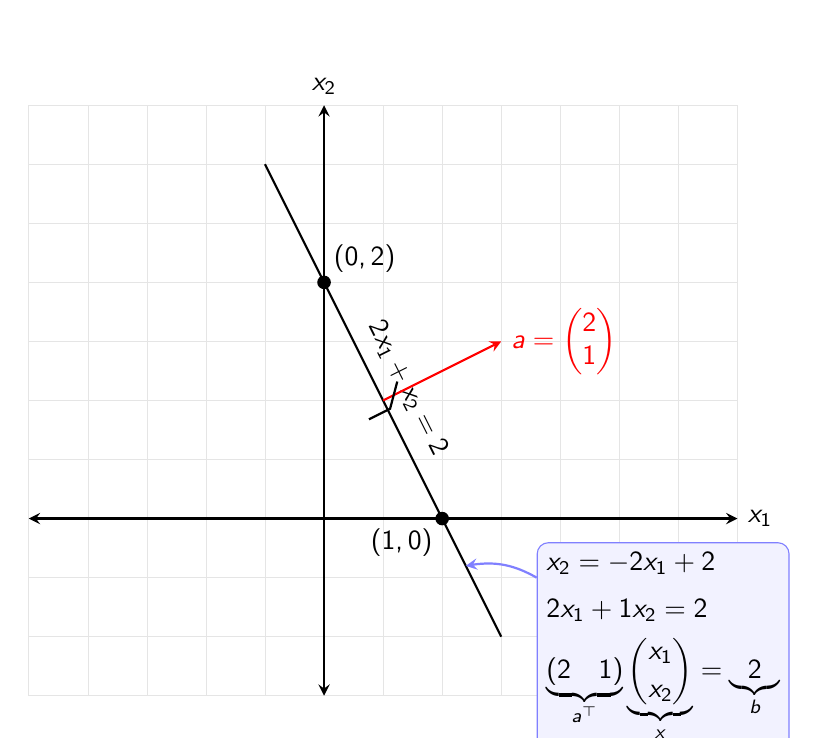
\begin{tikzpicture}[scale=1.5, >=stealth]
			% Grid
			\draw[step=0.5cm, gray!20, very thin] (-2.5,-1.5) grid (3.5,3.5);
			
			% Axes
			\draw[<->, thick] (-2.5,0) -- (3.5,0) node[right] {$x_1$};
			\draw[<->, thick] (0,-1.5) -- (0,3.5) node[above] {$x_2$};
			
			% The Line: 2x1 + x2 = 2  => x2 = -2x1 + 2
			% Intercepts: (1,0) and (0,2)
			% Plot from x1 = -0.5 to 1.5
			% x = -0.5 => y = 3
			% x = 1.5 => y = -1
			\draw[thick, black] (-0.5, 3) -- (1.5, -1) node[midway, sloped, above, yshift=2pt] {$2x_1 + x_2 = 2$};
			
			% Intercept Points
			\filldraw (0,2) circle (1.5pt) node[above right] {$(0,2)$};
			\filldraw (1,0) circle (1.5pt) node[below left] {$(1,0)$};
			
			% Normal Vector calculation
			\coordinate (P) at (0.5, 1);
			\draw[->, red, thick] (P) -- ++(1, 0.5) node[right] {$a = \begin{pmatrix} 2 \\ 1 \end{pmatrix}$};
			
			% Right angle marker
			\draw[thick] ($(P)!0.2cm!-63.4:(1.5,-1)$) -- ++(26.6:0.2) -- ($(P)!0.2cm!26.6:(1.5,1.5)$);
			
			% Annotation Box (Blue rounded rectangle)
			\node[draw=blue!50, fill=blue!5, rounded corners, align=left, anchor=north west] 
			at (1.8, -0.2) {
				$x_2 = -2x_1 + 2$ \\[0.5em]
				$2x_1 + 1x_2 = 2$ \\[0.5em]
				$\underbrace{(2 \quad 1)}_{a^\top} \underbrace{\binom{x_1}{x_2}}_{x} = \underbrace{2}_{b}$
			};
			
			% Curved arrow from box to line
			\draw[->, blue!50, thick, bend right=20] (1.8, -0.5) to (1.2, -0.4);
			
		\end{tikzpicture}
		\captionof{figure}{Geometric example of the hyperplane $2x_1 + x_2 = 2$. The normal vector $a=(2,1)^\top$ determines the orientation of the line.}
		\label{fig:example_hyperplane}
	\end{center}
	
	
	
\end{examplebox}



\begin{defnbox}{Polyhedron}
	Let $a_i \in \mathbb{R}^n$ and $b_i \in \mathbb{R}$ for $i=1,\dots,m$.  
	A \emph{polyhedron} $P \subset \mathbb{R}^n$ is the intersection of a finite
	number of closed half–spaces,
	\[
	P := \{ x \in \mathbb{R}^n \mid a_i^\top x \le b_i,\; i = 1,\dots,m \}.
	\]
	If we collect the row vectors $a_i^\top$ into a matrix
	$A := [a_1,\dots,a_m]^\top \in \mathbb{R}^{m \times n}$ and
	$b := [b_1,\dots,b_m]^\top \in \mathbb{R}^m$, then we may write
	\[
	P := \{ x \in \mathbb{R}^n \mid Ax \le b\},
	\]
	where the inequality is understood row–wise.
\end{defnbox}

\begin{defnbox}{Polytope}
	A \emph{polytope} is a bounded polyhedron, that is, a polyhedron which is
	contained in a ball of finite radius.
\end{defnbox}

\begin{alertbox}{Important observation}
	Any intersection of convex sets is convex. Each closed half–space
	$\{x \mid a_i^\top x \le b_i\}$ is convex, therefore every polyhedron
	(and hence every polytope) is a convex set. However, union of convex sets are not convex in general.
\end{alertbox}

\begin{examplebox}{Numerical Example: Defining a Polytope}
	
	Consider the set $P \subset \mathbb{R}^2$ defined by the inequalities
	\begin{align*}
		x_1 &\ge 0, &
		x_2 &\ge 0, \\
		x_1 &\le 3, &
		x_2 &\le 2, \\
		x_1 + x_2 &\le 4.
	\end{align*}
	We can rewrite these in the standard form $Ax \le b$ as
	\[
	A=
	\begin{bmatrix}
		-1 & 0 \\
		0 &-1 \\
		1 & 0 \\
		0 & 1 \\
		1 & 1
	\end{bmatrix},
	\qquad
	b=
	\begin{bmatrix}
		0 \\ 0 \\ 3 \\ 2 \\ 4
	\end{bmatrix},
	\qquad
	P := \{x\in\mathbb{R}^2 \mid Ax \le b\}.
	\]
	The intersection of these half–spaces is a bounded polygon with vertices
	\[
	\{(0,0),\ (3,0),\ (3,1),\ (2,2),\ (0,2)\},
	\]
	so $P$ is a polytope.
	
	The polytope $P$ can be visualised in the $(x_1,x_2)$–plane as shown in Figure~\ref{fig:polyhedron}:
	
	\begin{center}
	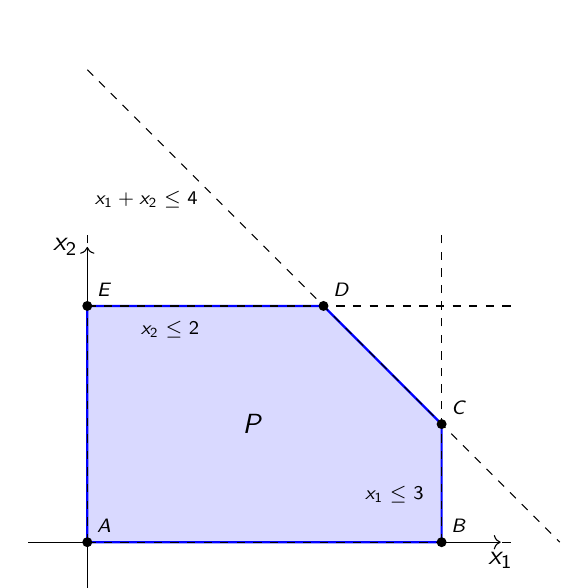
\begin{tikzpicture}[scale=1.5]
		% Axes
		\draw[->] (-0.5,0) -- (3.5,0) node[below] {$x_1$};
		\draw[->] (0,-0.5) -- (0,2.5) node[left] {$x_2$};
		
		% Feasible region (polytope)
		\fill[blue!15]
		(0,0) -- (3,0) -- (3,1) -- (2,2) -- (0,2) -- cycle;
		
		\draw[thick,blue]
		(0,0) -- (3,0) -- (3,1) -- (2,2) -- (0,2) -- cycle;
		
		% Constraint lines (optional, dashed)
		\draw[dashed] (0,0) -- (3.6,0);          % x2 = 0
		\draw[dashed] (0,0) -- (0,2.6);          % x1 = 0
		\draw[dashed] (3,0) -- (3,2.6);          % x1 = 3
		\draw[dashed] (0,2) -- (3.6,2);          % x2 = 2
		\draw[dashed] (0,4) -- (4,0);            % x1 + x2 = 4
		
		% Vertex labels
		\foreach \x/\y/\name in {0/0/A, 3/0/B, 3/1/C, 2/2/D, 0/2/E}
		\fill (\x,\y) circle (1.2pt) node[above right] {\scriptsize $\name$};
		
		% Text labels for half-spaces
		\node at (0.7,1.8) {\scriptsize $x_2 \le 2$};
		\node at (2.6,0.4) {\scriptsize $x_1 \le 3$};
		\node at (0.5,2.9) {\scriptsize $x_1 + x_2 \le 4$};
		
		\node at (1.4,1.0) {$P$};
	\end{tikzpicture}
	\captionof{figure}{Intersection of half spaces is a convex polyhedron.}
	\label{fig:polyhedron}
	\end{center}
	
\end{examplebox}


\subsection{Convex Functions}

Let $S$ be a convex subset of a vector space. We define the properties of functions mapping $S$ to the real numbers $\mathbb{R}$ as follows.

\begin{defnbox}{Convex Function}
	A function $f: S \rightarrow \mathbb{R}$ is said to be \textbf{convex} if $S$ is convex and the following inequality holds for all $z_1, z_2 \in S$ and for all $\lambda \in [0, 1]$:
	\begin{equation}
		f(\lambda z_1 + (1 - \lambda)z_2) \leq \lambda f(z_1) + (1 - \lambda)f(z_2)
	\end{equation}
	Geometrically, this means that the line segment connecting any two points on the graph of the function lies above or on the graph between the two points.
\end{defnbox}
	
\begin{defnbox}{Concave Function}
	A function $f: S \rightarrow \mathbb{R}$ is \textbf{concave} if $S$ is convex and $-f$ is a convex function. Equivalently, the inequality in the definition of convexity is reversed.
\end{defnbox}


The concept of convexity is illustrated in Figure \ref{fig:convex_func}. The curve represents the function $f$. The red secant line connects two points $(z_1, f(z_1))$ and $(z_2, f(z_2))$. For a convex function, the value of the function evaluated at a weighted average of two points (the black dot on the curve) is always less than or equal to the weighted average of the function values (the black dot on the red line).

\begin{figure}[h]
	\centering
	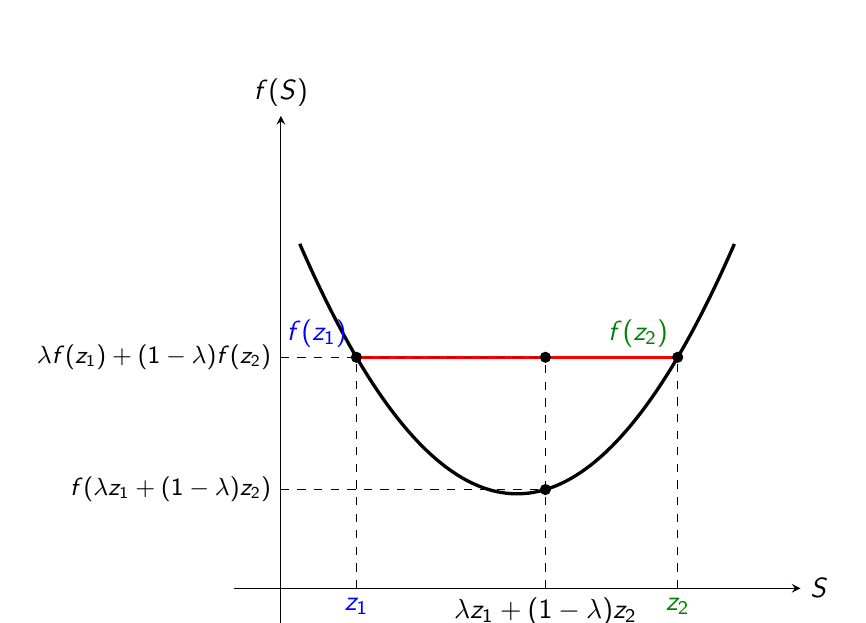
\begin{tikzpicture}[scale=1.2, >=stealth]
		% Define the function (simple parabola shifted)
		\def\func(#1){0.5*(#1-2.5)*(#1-2.5) + 1}
		
		% Define points
		\def\zOne{0.8}
		\def\zTwo{4.2}
		\def\zMix{2.8} 
		
		% Calculate y values
		\pgfmathsetmacro{\yOne}{\func(\zOne)}
		\pgfmathsetmacro{\yTwo}{\func(\zTwo)}
		\pgfmathsetmacro{\yCurve}{\func(\zMix)}
		
		% Calculate y value on the secant line (linear interpolation)
		% slope m = (y2 - y1) / (z2 - z1)
		% y_line = y1 + m * (zMix - z1)
		\pgfmathsetmacro{\slope}{(\yTwo - \yOne) / (\zTwo - \zOne)}
		\pgfmathsetmacro{\yLine}{\yOne + \slope * (\zMix - \zOne)}
		
		% Coordinate Axes
		\draw[->] (-0.5,0) -- (5.5,0) node[right] {$S$};
		\draw[->] (0,-0.5) -- (0,5) node[above] {$f(S)$};
		
		% Draw the curve
		\draw[line width=1.2pt] plot[domain=0.2:4.8, samples=100] (\x, {0.5*(\x-2.5)*(\x-2.5) + 1});
		
		% Draw the secant line (Red)
		\draw[red, line width=1.2pt] (\zOne, \yOne) -- (\zTwo, \yTwo);
		
		% Draw points
		\filldraw (\zOne, \yOne) circle (1.5pt) node[above left, text=blue] {$f(z_1)$};
		\filldraw (\zTwo, \yTwo) circle (1.5pt) node[above left, text=green!50!black] {$f(z_2)$};
		\filldraw (\zMix, \yCurve) circle (1.5pt); % Point on curve
		\filldraw (\zMix, \yLine) circle (1.5pt);  % Point on line
		
		% Dashed projection lines (Vertical)
		\draw[dashed] (\zOne, 0) -- (\zOne, \yOne);
		\draw[dashed] (\zTwo, 0) -- (\zTwo, \yTwo);
		\draw[dashed] (\zMix, 0) -- (\zMix, \yCurve); % To curve
		\draw[dashed] (\zMix, \yCurve) -- (\zMix, \yLine); % Connect curve to line
		
		% Dashed projection lines (Horizontal)
		\draw[dashed] (0, \yCurve) -- (\zMix, \yCurve);
		\draw[dashed] (0, \yLine) -- (\zMix, \yLine);
		
		% Labels on X-axis
		\node[below, text=blue] at (\zOne, 0) {$z_1$};
		\node[below, text=green!50!black] at (\zTwo, 0) {$z_2$};
		\node[below] at (\zMix, 0) {$\lambda z_1 + (1-\lambda)z_2$};
		
		% Labels on Y-axis
		\node[left, font=\small] at (0, \yLine) {$\lambda f(z_1) + (1-\lambda)f(z_2)$};
		\node[left, font=\small] at (0, \yCurve) {$f(\lambda z_1 + (1-\lambda)z_2)$};
		
	\end{tikzpicture}
	\caption{Geometric interpretation of a convex function. The line segment connecting any two points on the curve lies above the function values.}
	\label{fig:convex_func}
\end{figure}



\section{Classification of Optimisation Problems}

In the previous sections, we defined the general anatomy of an optimisation problem (Variables, Objectives, Constraints). However, in engineering practice, identifying the specific \textit{class} of a problem is critical.

Different classes of problems require different numerical algorithms (solvers). For instance, solving a linear problem is instantaneous, whereas solving a non-convex nonlinear problem might take hours or fail completely. If we can mathematically massage our engineering problem to fit a standard form, we can solve it efficiently using off-the-shelf software.

We typically classify problems in two ways:
\begin{enumerate}
	\item By the \textbf{existence and type of constraints} (Constrained vs. Unconstrained).
	\item By the \textbf{mathematical structure} of the cost and constraint functions (Linear, Quadratic, Nonlinear).
\end{enumerate}

\subsection{Classification I: Existence of Constraints}

The most fundamental distinction is whether the decision variables are restricted by boundaries.

\subsubsection{Unconstrained Optimisation}

An unconstrained problem is one where the decision variables can take any value in the Euclidean space $\mathbb{R}^n$. There are no boundaries, fences, or rules limiting $x$.

\begin{equation}
	\min_{x \in \mathbb{R}^n} J(x)
\end{equation}

\paragraph*{Visualising Unconstrained Problems: Level Curves}

When dealing with $n$ variables, the function $J(x)$ describes a surface in $n+1$ dimensions. This is hard to visualise. Instead, we use {Level Curves} (or contour lines). A level curve is a hypersurface defined by $J(x) = c$, where $c$ is a constant scalar. This is exactly like looking at a topographical map of a mountain; each line represents a constant height.

\begin{examplebox}{Unconstrained Example: The Bowl}
	Consider the simple quadratic function:
	\[ J(x) = x_1^2 + x_2^2 \]
	Here, $x = [x_1, x_2]^\top$. We want to find the minimum. The level curves are circles where $x_1^2 + x_2^2 = c$.
	\begin{itemize}
		\item If $c=5$, the curve is a circle of radius $\sqrt{5}$.
		\item If $c=0$, the curve is a single point at the origin.
	\end{itemize}
	Figure~\ref{fig:level_curves} shows several level curves $J=2$, $J=6$, $J=12$ and $J=20$.
	
	
	\begin{center}
		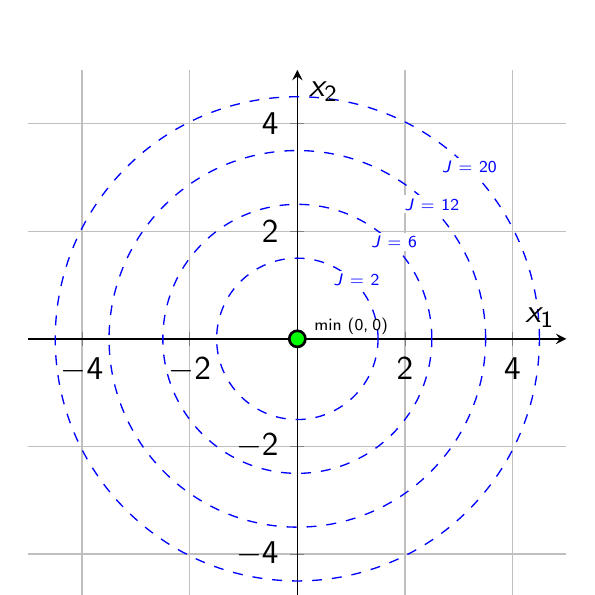
\begin{tikzpicture}[scale=1.2]
			\begin{axis}[
				axis lines = middle,
				xlabel = $x_1$,
				ylabel = $x_2$,
				xmin = -5, xmax = 5,
				ymin = -5, ymax = 5,
				axis equal image,
				grid = major,
				xtick = {-4,-2,0,2,4},
				ytick = {-4,-2,0,2,4},
				]
				% Draw contours (circles)
				\draw[blue, dashed] (axis cs:0,0) circle [radius=1.5]; % f approx 2.25
				\draw[blue, dashed] (axis cs:0,0) circle [radius=2.5]; % f approx 6.25
				\draw[blue, dashed] (axis cs:0,0) circle [radius=3.5]; % f approx 12.25
				\draw[blue, dashed] (axis cs:0,0) circle [radius=4.5]; % f approx 20.25
				
				% Labels for the contours
				\node[blue, font=\tiny, fill=white, inner sep=1pt] at (axis cs: 1.1, 1.1) {$J=2$};
				\node[blue, font=\tiny, fill=white, inner sep=1pt] at (axis cs: 1.8, 1.8) {$J=6$};
				\node[blue, font=\tiny, fill=white, inner sep=1pt] at (axis cs: 2.5, 2.5) {$J=12$};
				\node[blue, font=\tiny, fill=white, inner sep=1pt] at (axis cs: 3.2, 3.2) {$J=20$};
				
				% The Minimum
				\draw[fill=green, draw=black, thick] (axis cs:0,0) circle [radius=0.15];
				\node[anchor=north west] at (axis cs:0.1, 0.6) {\tiny min $(0,0)$};
			\end{axis}
		\end{tikzpicture}
		\captionof{figure}{Level Curves of $J(x) = x_1^2 + x_2^2$.}
		\label{fig:level_curves}
	\end{center}
	
	The optimiser searches for the level curve with the smallest possible $c$. Geometrically, this is the centre of the concentric circles.
\end{examplebox}

\subsubsection{Constrained Optimisation}

In most engineering applications, particularly MPC, we are restricted. Valves cannot open more than 100\%, and tanks cannot hold negative volume. This leads to constrained optimisation, where $x$ must belong to a specific feasible set $S$. We classify these based on how the set $S$ is defined.

\paragraph{Type A: Equality Constraints}

An equality constrained problem restricts the decision variables to lie strictly on a specific curve or surface ($h(x)=0$). The solver is not allowed to choose any point off this line. Mathematically, this reduces the dimension of the search space.

\begin{examplebox}{Equality Constraints: The Tangent Point}
	\textbf{Problem Statement:} 
	Minimise the same quadratic function as before, but subject to a linear equality constraint.
	
	\begin{equation*}
		\begin{aligned}
			& \min_{x} \quad  J(x) = x_1^2 + x_2^2 \\
			\text{subject to:} &\\
			 & h(x) = x_1 + 2x_2 - 4 = 0
		\end{aligned}
	\end{equation*}
	
	\textbf{Visualisation:}
	This problem is visualised in Figure~\ref{fig:optimization_with_constraints}. 
	\begin{center}
		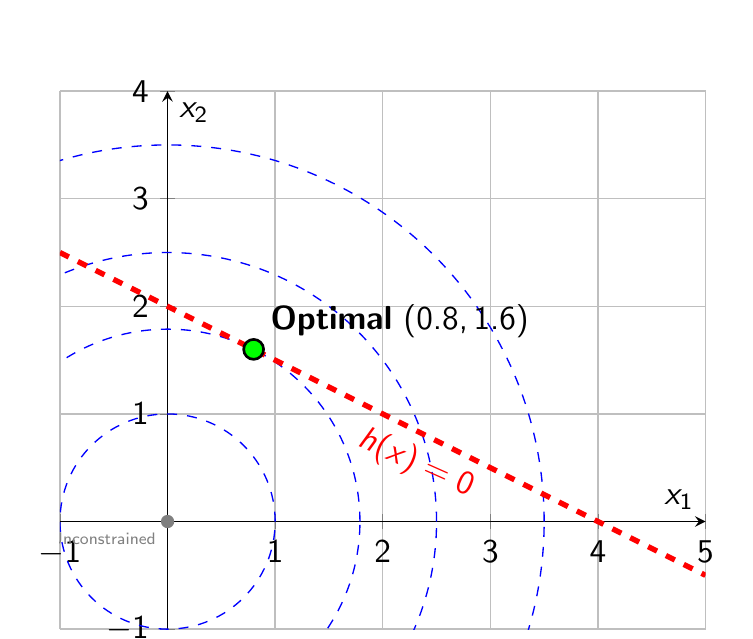
\begin{tikzpicture}[scale=1.2]
			\begin{axis}[
				axis lines = middle,
				xlabel = $x_1$,
				ylabel = $x_2$,
				xmin = -1, xmax = 5,
				ymin = -1, ymax = 4,
				axis equal image,
				grid = major,
				]
				% 1. Draw Level Curves
				\draw[blue, dashed] (axis cs:0,0) circle [radius=1];
				\draw[blue, dashed] (axis cs:0,0) circle [radius=1.788];
				\draw[blue, dashed] (axis cs:0,0) circle [radius=2.5];
				\draw[blue, dashed] (axis cs:0,0) circle [radius=3.5];
				
				% 2. Draw Constraint Line: x1 + 2x2 - 4 = 0  =>  x2 = 2 - 0.5*x1
				\addplot[domain=-1:5, samples=2, color=red, ultra thick, dashed] {2 - 0.5*x};
				\node[red, rotate=-24, anchor=south] at (axis cs: 2.2, 0.3) {$h(x)=0$};
				
				% 3. Draw Unconstrained Minimum (Origin)
				\fill[gray] (axis cs:0,0) circle (2pt) node[below left] {\tiny Unconstrained};
				
				% 4. Draw Constrained Minimum
				\fill[green, draw=black, thick] (axis cs:0.8, 1.6) circle (3pt);
				\node[anchor=south west] at (axis cs:0.85, 1.6) {\textbf{Optimal} $(0.8, 1.6)$};
			\end{axis}
		\end{tikzpicture}
		\captionof{figure}{Minimising $J(x)$ on the line $h(x)=0$}.
		\label{fig:optimization_with_constraints}
	\end{center}
	
	\solution
	The optimal point is found where the constraint line is exactly {tangent} to a level curve.
\end{examplebox}

\paragraph{Type B: Inequality Constraints}

Unlike equality constraints, inequality constraints confine the solution to a \textit{region} (a set of alternatives). The optimal solution may lie on the boundary of this region (active constraint) or strictly inside it (inactive constraint).

\begin{examplebox}{Inequality Constraints: The Feasible Region}
	Minimise the cost function $J(x) = x_1^2 + x_2^2$, subject to four linear inequalities:
	\[
	\begin{aligned}
		-x_1 - 2x_2 + 5 &\leq 0 \\
		2x_1 + x_2 - 5 &\leq 0 \\
		x_1 \ge 0, \ x_2 &\ge 0
	\end{aligned}
	\]
	\solution
	

	Visualisation is excellent for understanding, but to get numerical answers, we use software. In this course, we utilise \textbf{YALMIP}, an open source MATLAB toolbox that allows us to write optimisation problems using syntax that looks almost identical to the mathematics.
	
	The workflow always follows three steps: 
	\begin{center}
	Define Optimisation Variables $\to$ Define Model $\to$ Solve.
	\end{center}

	
	\begin{lstlisting}[language=Matlab]
		% 1. Define Decision Variables
		% 'sdpvar' creates a symbolic variable that YALMIP tracks.
		x = sdpvar(2,1); 
		
		% 2. Define the Objective Function
		J = x(1)^2 + x(2)^2;
		
		% 3. Define Constraints
		% We create a list of inequalities using standard MATLAB brackets.
		Constraints = [ -x(1) - 2*x(2) + 5 <= 0, ...
								2*x(1) +   x(2) - 5 <= 0, ...
								x(1) >= 0, ...
								x(2) >= 0 ];
		
		% 4. Call the Solver
		% We ask YALMIP to minimise J subject to Constraints
		optimize(Constraints, J);
		
		% 5. Extract Result
		% The symbolic variable 'x' now holds the optimal value.
		x_star = value(x) % Result: (1, 2)
	\end{lstlisting}
	
	\textbf{Visualisation:}
	Geometrically, the optimiser ``expands'' the level curves (blue circles) from the origin until they first touch the feasible region (grey polygon).
	
	\begin{center}
		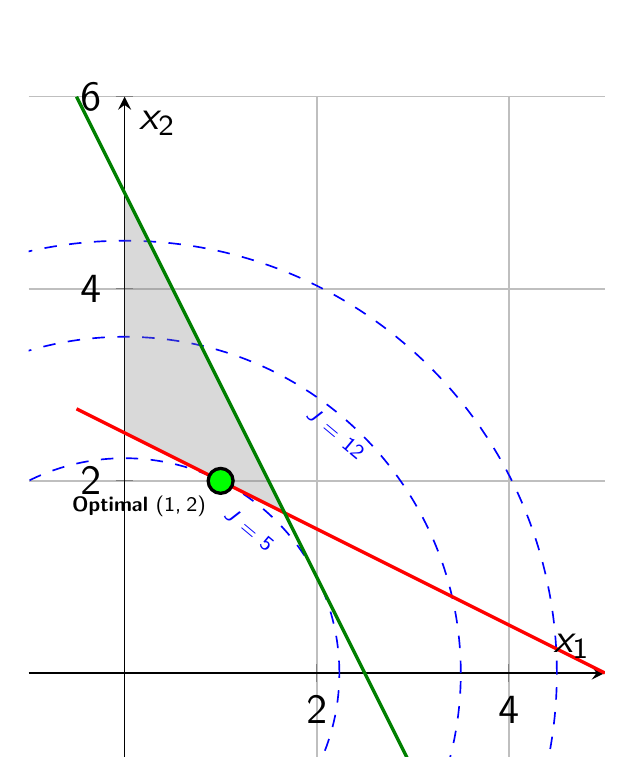
\begin{tikzpicture}[scale=1.5]
			\begin{axis}[
				axis lines = middle,
				xlabel = $x_1$,
				ylabel = $x_2$,
				xmin = -1, xmax = 5,
				ymin = -1, ymax = 6,
				axis equal image,
				grid = major,
				]
				
				% 1. Level Curves
				\draw[blue, dashed] (axis cs:0,0) circle [radius=2.236]; % Radius sqrt(5) approx 2.23
				\draw[blue, dashed] (axis cs:0,0) circle [radius=3.5];
				\draw[blue, dashed] (axis cs:0,0) circle [radius=4.5];
				
				\node[rotate= -40, blue, font=\tiny] at (axis cs: 1.3, 1.5) {$J=5$};
				\node[rotate= -40, blue, font=\tiny] at (axis cs: 2.2, 2.5) {$J=12$};
				% 2. Feasible Region
				\fill[gray, opacity=0.3] (axis cs:0, 2.5) -- (axis cs:0, 5) -- (axis cs:1.666, 1.666) -- cycle;
				
				% 3. Constraint Lines
				\addplot[domain=-0.5:5, color=red, thick] {2.5 - 0.5*x};
				\addplot[domain=-0.5:3, color=green!50!black, thick] {5 - 2*x};
				
				% 4. Optimal Point
				\fill[green, draw=black, thick] (axis cs:1, 2) circle (3pt);
				\node[anchor=north east] at (axis cs:1, 2) {{\tiny \textbf{Optimal} $(1, 2)$}};
			\end{axis}
		\end{tikzpicture}
	\end{center}
\end{examplebox}
\paragraph{Type C: General Constraints}

In the most general case, a problem contains both equality and inequality constraints. The solver must find a solution that lies inside the inequality region \textbf{and} lies exactly on the equality curve.

Geometrically, the feasible set is the intersection of the regions defined by all constraints. This often effectively reduces the dimensionality of the search space.

\begin{examplebox}{General Constraints: Mixing Equalities and Inequalities}
	\textbf{Problem Statement:}
	Consider a scenario where we must satisfy both safety limits (inequalities) and strict physical laws (equalities). We wish to minimise the quadratic cost $J(x) = x_1^2 + x_2^2$ subject to:
	\begin{equation*}
		\begin{aligned}
			\text{s.t.} \quad & -x_1 - 2x_2 + 5 \leq 0 \\
			& 2x_1 + x_2 - 5 \leq 0 \\
			& x_1 \ge 0, \quad x_2 \ge 0 \\
			& x_1 + 2x_2 - 7 = 0 \quad {(Equality)}
		\end{aligned}
	\end{equation*}
	
	\solution
	
	\textbf{YALMIP Implementation:}
	When translating this into code, pay close attention to the syntax for the equality constraint. In MATLAB, a single equals sign (\texttt{=}) represents assignment (e.g., setting a variable's value). To represent a logical equality condition ($h(x)=0$), we must use the double equals sign (\texttt{==}).
	
	\begin{lstlisting}[language=Matlab]
		% 1. Define Variables and Objective
		x = sdpvar(2,1);
		J = x(1)^2 + x(2)^2;
		
		% 2. Define Inequality Constraints (The Feasible Region)
		g1 = [-x(1) - 2*x(2) + 5 <= 0]; 
		g2 = [ 2*x(1) + x(2) - 5 <= 0]; 
		g3 = [x(1) >= 0];               
		g4 = [x(2) >= 0];     
		
		% 3. Define Equality Constraint (The Manifold)
		% Note the use of '==' for logical equality
		h  = [x(1) + 2*x(2) - 7 == 0];
		
		% 4. Combine and Solve
		Constraints = [g1, g2, g3, g4, h];
		optimize(Constraints, J);
		
		x_star = value(x) % Result: (1, 3)
	\end{lstlisting}
	
	\textbf{Visualisation and Analysis:}
	The geometry of this problem is illustrated in Figure~\ref{fig:Intersection_of_constraints}.
	\begin{itemize}
		\item The inequalities form the grey triangular region.
		\item The equality constraint is represented by the orange dashed line.
	\end{itemize}
	A valid solution must satisfy \textit{both} conditions. Therefore, the feasible set is reduced to the specific line segment where the orange line slices through the grey triangle.
	
	\begin{center}
		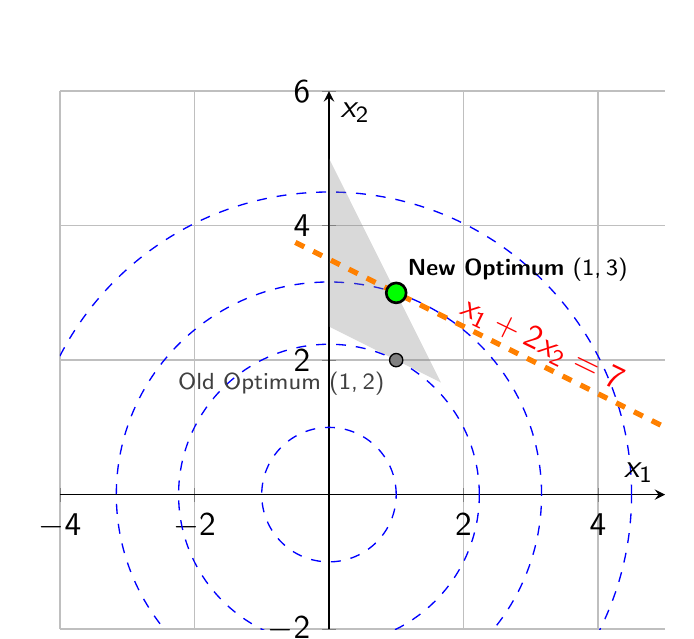
\begin{tikzpicture}[scale=1.2]
			\begin{axis}[
				axis lines = middle,
				xlabel = $x_1$,
				ylabel = $x_2$,
				xmin = -4, xmax = 5,
				ymin = -2, ymax = 6,
				axis equal image,
				grid = major,
				]
				
				% 1. Level Curves
				\draw[blue, dashed] (axis cs:0,0) circle [radius=2.236]; % f=5 (Old optimum)
				\draw[blue, dashed] (axis cs:0,0) circle [radius=3.162]; % f=10 (New optimum)
				\draw[blue, dashed] (axis cs:0,0) circle [radius=4.5];
				\draw[blue, dashed] (axis cs:0,0) circle [radius=1];
				
				
				% 2. Feasible Region (Grey Triangle from Inequalities)
				\fill[gray, opacity=0.3] (axis cs:0, 2.5) -- (axis cs:0, 5) -- (axis cs:1.666, 1.666) -- cycle;
				
				% 3. Equality Constraint Line: x + 2y = 7 -> y = 3.5 - 0.5x
				\addplot[domain=-0.5:5, color=orange, ultra thick, dashed] {3.5 - 0.5*x};
				\node[red, font=\normalsize, rotate=-26, anchor=south] at (axis cs: 3, 1.9) { $x_1 + 2x_2 = 7$};
				
				% 4. Previous Optimal Point (Inequalities only)
				\fill[gray, draw=black] (axis cs:1, 2) circle (2pt);
				\node[darkgray, font=\scriptsize, anchor=north east] at (axis cs:1, 2) {Old Optimum $(1, 2)$};
				
				% 5. New Optimal Point
				\fill[green, draw=black, thick] (axis cs:1, 3) circle (3pt);
				\node[anchor=south west, font=\scriptsize] at (axis cs:1, 3) { \textbf{New Optimum} $(1, 3)$};
				
			\end{axis}
		\end{tikzpicture}
		\captionof{figure}{Intersection of Equality and Inequalities}
		\label{fig:Intersection_of_constraints}
	\end{center}
	
	\textbf{The Cost of Constraints:}
	In the previous example (inequalities only), the optimiser could reach the point $(1,2)$, which yielded a cost of $J=5$. 
	
	However, the new equality constraint forces the solution to lie on the line $x_1 + 2x_2 = 7$. The point $(1,2)$ is no longer valid because $1 + 2(2) = 5 \neq 7$. The solver is forced to move further away from the origin to satisfy this new rule, settling at $(1,3)$ with a higher cost of $J=10$.
	
	This illustrates a fundamental rule of engineering optimisation: {Adding constraints generally worsens (increases) the minimum cost}, as it restricts the freedom of the solver to find "cheaper" solutions.
\end{examplebox}

\subsection{Classification II: Mathematical Structure}

Optimisation problems vary greatly in difficulty depending on the structure of their objective functions and constraints. In this section we review some of the most commonly encountered problem classes, beginning with those that are considered \emph{easy} from a computational point of view, and progressing to problems that are, in general, far more challenging to solve.

% --------------------------------------------------------
\subsubsection{Linear Programmes (LPs)}

Linear Programmes constitute one of the most fundamental classes of convex optimisation problems. Both the objective and the constraints are linear:
\begin{align*}
	&\min_{x} \; c^{\top} x \\
	 \text{subject to: } & \\
	&Gx \le h \\
	&Ax = b 
\end{align*}

The feasible set of an LP is a polyhedron, and the optimum, when it exists, is attained at an extreme point (vertex) of this polyhedron. Linear optimisation on a polytope may be visualised as shifting parallel hyperplanes of constant cost until they touch the feasible region. Figure~\ref{fig:LP} shows a 2D example where the polytope  corresponds to the closed area modelled by $Gx\le h$ and dashed lines shows the cost for different values of $c^\top x$.

\begin{figure}[!htb]
	\centering
	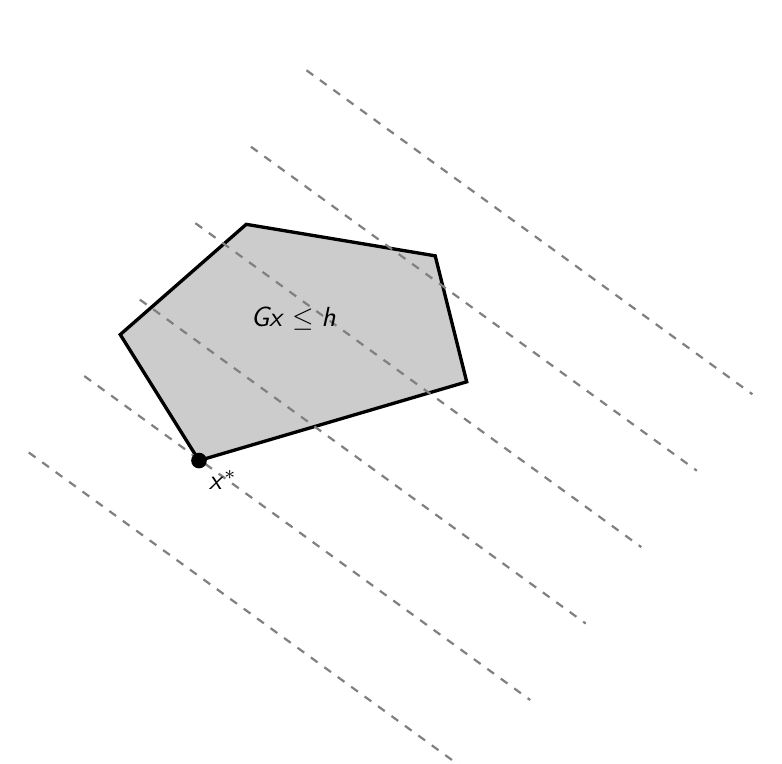
\begin{tikzpicture}[scale=2]
		
		% Define the vertices of the pentagon (polytope P)
		\coordinate (A) at (0.5, 0);
		\coordinate (B) at (0, 0.8);
		\coordinate (C) at (0.8, 1.5);
		\coordinate (D) at (2, 1.3);
		\coordinate (E) at (2.2, 0.5);
		
		% Draw and fill the polytope
		\fill[gray!40] (A) -- (B) -- (C) -- (D) -- (E) -- cycle;
		\draw[line width=1.2pt] (A) -- (B) -- (C) -- (D) -- (E) -- cycle;
		
		% Draw the dashed parallel lines (level sets of objective function) - AFTER the polytope
		\foreach \y in {-0.3, 0.3, 0.9, 1.5, 2.1, 2.7} {
			\draw[dashed, gray, rotate = -36, thick] (-0.5, \y) -- (3, \y);
		}
		
		% Label the polytope
		\node at (1.1, 0.9) { $Gx \le h$};
		
		% Mark the optimal point
		\node[circle, fill=black, inner sep=2pt] at (A) {};
		\node[below right] at (A) {$x^*$};
		
		
	\end{tikzpicture}
	\caption{Linear optimisation on a polytope.}
	\label{fig:LP}
\end{figure}

\begin{examplebox}{Linear Programme: Minimum-Effort Steady State}
	
	\textbf{The Goal:}
	Consider a discrete-time linear system $$x_{k+1} = Ax_k + Bu_k$$ We wish to find a steady-state pair $(x_{\mathrm{ss}}, u_{\mathrm{ss}})$ (an equilibrium point where the system stays at rest ($x_{k+1} = x_k$)) subject to safety constraints.
	
	Crucially, among all possible valid equilibria, we want to find the one that requires the \emph{least control effort}. In engineering (e.g., satellite thrusters), "effort" is often quantified by fuel consumption, which corresponds to the sum of the absolute values of the inputs.
	
	\textbf{1. The 1-Norm and Notation:}
	Mathematically, we want to minimise the \textbf{1-norm} of the input vector $u \in \mathbb{R}^m$:
	\begin{equation}
		\|u\|_1 = \sum_{i=1}^{m} |u_i| = |u_1|+|u_2|+\cdots + |u_m|
	\end{equation}
	However, the absolute value function $|u|$ is non-linear. Standard LP solvers cannot handle it directly. To solve this, we use a standard optimisation trick involving the vector $1$.
	\begin{itemize}
		\item Let $1$ be a column vector of ones: $1 = [1, 1, \dots, 1]^\top$.
		\item Then $1^\top t$ is simply the sum of the elements of vector $t$: $\sum t_i$.
	\end{itemize}
	
	\textbf{2. The Epigraph Trick:}
	We introduce an auxiliary decision vector $t \in \mathbb{R}^m$. We constrain $t$ to be an upper bound on the magnitude of $u$:
	\begin{equation}
		-t_i \le u_i \le t_i \implies |u_i| \le t_i
	\end{equation}
	If we minimise the sum of elements in $t$ (i.e., $\min 1^\top t$), the solver will squeeze $t_i$ down until $t_i = |u_i|$. This effectively minimises $|u_i|$ using only linear inequalities.
	
	\textbf{3. The Formulation:}
	We can now pose the full Linear Programme. The decision variables are the input $u$, the state $x_{\mathrm{ss}}$, and the auxiliary bound $t$.
	
	\[
	\begin{aligned}
		&\min_{u,\, x_{\mathrm{ss}},\, t} \quad   1^\top t  && \text{(Minimise total fuel/effort)}\\
		\text{subject to:} &&& \\ 
		& (I-A)x_{\mathrm{ss}} - Bu = 0, && \text{(Equilibrium Physics)}\\
		& G\,x_{\mathrm{ss}} \le h, && \text{(Safety Constraints)}\\
		& u_{\min} \le u \le u_{\max}, && \text{(Actuator Limits)}\\
		& -t \le u \le t. && \text{(Norm Linearisation)}
	\end{aligned}
	\]
	
	This formulation allows us to find the most efficient operating point for the system using extremely fast and reliable Linear Programming solvers.
\end{examplebox}

\begin{examplebox}{Stigler's Diet Problem:}
	
The Stigler Diet Problem is a classic linear optimisation problem. The objective is to determine the most cost-effective daily diet that meets specific nutritional requirements using a limited set of foods.

In this simplified 2D version, we consider two food items: {Corn} and {Wheat Bread}. We aim to minimise the total daily cost while satisfying constraints for {Energy (Calories)} and {Vitamin A}.

We first define the problem using general parameters and units.

\textbf{Decision Variables:}
\begin{itemize}
	\item $x_1$: Quantity of Corn [kg]
	\item $x_2$: Quantity of Bread [kg]
\end{itemize}

\textbf{Parameters:}
\begin{itemize}
	\item $c_1, c_2$: Price of food [\$/kg]
	\item $k_1, k_2$: Energy content [kcal/kg]
	\item $v_1, v_2$: Vitamin A content [$\mu$g/kg]
	\item $K_{min}, K_{max}$: Daily energy limits [kcal]
	\item $V_{min}, V_{max}$: Daily Vitamin A limits [$\mu$g]
\end{itemize}

\textbf{Optimisation Model:}
\begin{align*}
	\underset{x_1,\,x_2}{\text{min}} \quad & J(x) = c_1 x_1 + c_2 x_2 \\
	\text {Subject to:} \quad & K_{min} \leq k_1 x_1 + k_2 x_2 \leq K_{max} \\
	& V_{min} \leq v_1 x_1 + v_2 x_2 \leq V_{max} \\
	& x_1 \geq 0, \quad x_2 \geq 0
\end{align*}

Using the specific data provided for the problem:

\textbf{Data:}
\begin{itemize}
	\item Costs: $c_1 = 2.0$, $c_2 = 0.5$
	\item Energy: $k_1 = 750$, $k_2 = 650$ (Target: $2000 - 3000$ kcal)
	\item Vitamin A: $v_1 = 250$, $v_2 = 0$ (Target: $500 - 800$ $\mu$g)
\end{itemize}

Numerically, the problem can be stated as follows:

	\begin{align*}
			&\underset{x_1,x_2}{\min }  \quad J(x) = 2x_1 + 0.5x_2 & \\
			\text{Subject to:} &&\\
		&2000 \leq 750x_1 + 650x_2 \leq 3000 & \text{(Energy)} \\
		&500 \leq 250x_1 \phantom{{} + 650x_2} \leq 800 & \text{(Vitamin A)} \\
		& x_1 \geq 0, \quad x_2 \geq 0 & \text{(Nonnegativity)}
	\end{align*}
	Figure~\ref{fig:stigler2d} shows the feasible solution set along with the optimal solution that minimises the cost of nutrition. 
	
\begin{lstlisting}[language=Matlab, caption=Solving Stigler's Problem with YALMIP]
	clear; clc;
	
	x1 = sdpvar(1); % Corn (kg)
	x2 = sdpvar(1); % Bread (kg)
	
	Objective = 2*x1 + 0.5*x2;
	
	% 3. Define Constraints
	Constraints = [];
	Constraints = [Constraints, 2000 <= 750*x1 + 650*x2 <= 3000];
	Constraints = [Constraints, 500 <= 250*x1 <= 800];
	Constraints = [Constraints, x1 >= 0, x2 >= 0];
	
	% 'linprog' for LP; use 'quadprog' or 'osqp' for QP/SOCP variants.
	options = sdpsettings('verbose', 0, 'solver', 'linprog');
	sol = optimize(Constraints, Objective, options);
	
	if sol.problem == 0
		fprintf('Optimal Solution:\n');
		fprintf('x1 (Corn) : %.4f kg\n', value(x1));
		fprintf('x2 (Bread): %.4f kg\n', value(x2));
		fprintf('Min Cost  : $%.4f\n', value(Objective));
	else
		disp('Problem could not be solved.');
	end
\end{lstlisting}
\end{examplebox}
\begin{figure}[h!]
	\centering
	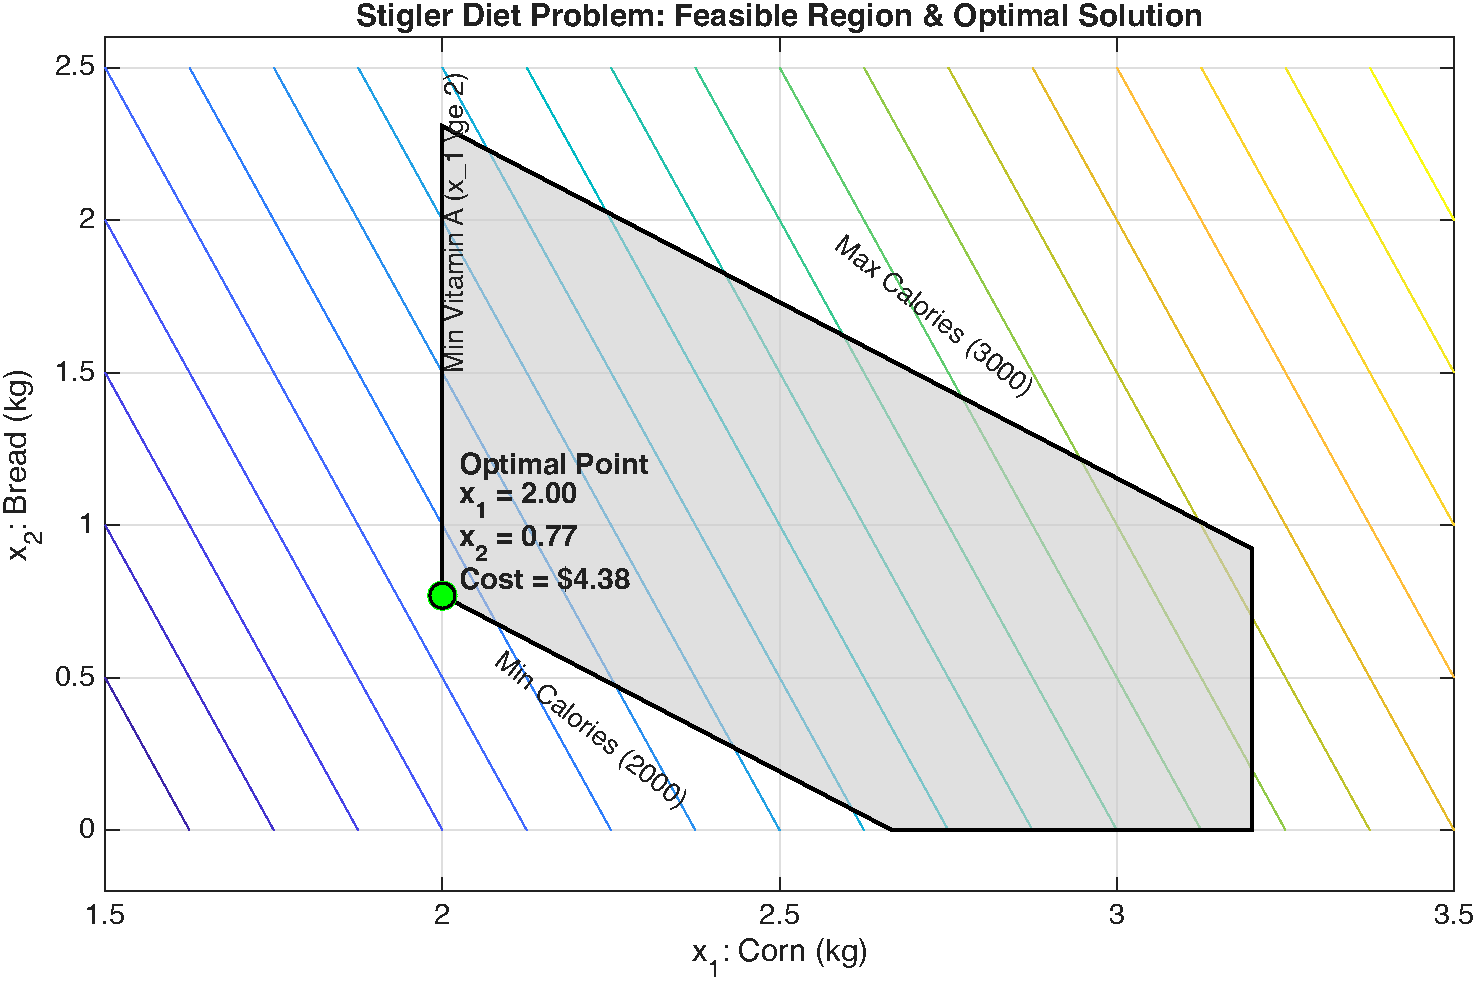
\includegraphics[width=0.7\linewidth]{Figures/Stigler2d}
	\caption{Numerical solution of the 2d Stigler problem in MATLAB.}
	\label{fig:stigler2d}
\end{figure}

% --------------------------------------------------------
\subsubsection{Convex Quadratic Programmes (QPs)}

Quadratic Programmes (QPs) extend linear optimisation by allowing a quadratic objective function whilst retaining linear equality and inequality constraints.
A QP takes the general form
\begin{align*}
	&\min_{x} \quad \frac{1}{2} x^{\top} P x + q^{\top} x \\ 
	 \text{subject to: } & \\
	 & Gx \le h \\ 
	 & Ax = b 
\end{align*}

where, $x\in \mathbb R^n$, $P \in \mathbb{R}^{n \times n}$, $q \in \mathbb{R}^n$, $G \in
\mathbb{R}^{m \times n}$, and $A \in \mathbb{R}^{p \times n}$.  
The feasible region defined by the linear constraints is always a polyhedron.

The QP is \emph{convex} if and only if the Hessian matrix $P$ is
positive semidefinite:
\[
P \succeq 0 .
\]
This is shown in Figure~\ref{fig:QP}.

\begin{notebox}{Tests for Positive Semidefiniteness ($P \succeq 0$)}
	For a \emph{symmetric} matrix \(P\), the following statements are equivalent and may be used to verify that \(P\) is positive semidefinite:
	
	\begin{enumerate}
		\item \textbf{Eigenvalues:} All eigenvalues of \(P\) are non-negative:
		\[
		\lambda_i(P) \ge 0, \qquad i=1,\dots,n.
		\]
		
		\item \textbf{Quadratic Form:} The quadratic form is non-negative for every vector \(z \in \mathbb{R}^n\):
		\[
		z^\top P z \ge 0, \qquad \forall z \in \mathbb{R}^n.
		\]
		
		\item \textbf{Principal Minors:} All \emph{principal minors} of \(P\) are non-negative.
		In other words, the determinant of every principal submatrix must satisfy
		\[
		\det(P_{\mathcal I,\mathcal I}) \ge 0
		\]
		for every index set \(\mathcal I \subseteq \{1,\dots,n\}\).
	\end{enumerate}
	
	\textbf{Important note:}  
	For \emph{positive definite} matrices \((P \succ 0)\), Sylvester's criterion states that it is enough to check that all \emph{leading principal minors} are strictly positive. However, for \emph{positive semidefinite} matrices \((P \succeq 0)\), checking only the leading principal minors is \emph{not} sufficient in general; one must check all principal minors, or use one of the equivalent tests above.

	(For a review of eigenvalues, definiteness, and related matrix concepts, see Appendix~\ref{app:linalg}.)
\end{notebox}

\begin{defnbox}{Hessian}
	The Hessian matrix, denoted as $\nabla^2 f(x)$ or $H(x)$, collects all second-order partial derivatives of a scalar-valued function $f: \mathbb{R}^n \to \mathbb{R}$. If $x = [x_1, x_2, \dots, x_n]^\top$, the element in the $i$-th row and $j$-th column is given by:
	\begin{equation*}
		H_{ij} = \dfrac{\partial^2 f}{\partial x_i \partial x_j}
	\end{equation*}
\end{defnbox}

\begin{examplebox}{Example: Hessian}
	Consider a simple function of two variables:
	\[
	f(x) = 3x_1^2 + 2x_1 x_2 + 5x_2^2
	\]
	First, we find the gradient (first derivatives):
	\[
	\dfrac{\partial f}{\partial x_1} = 6x_1 + 2x_2, \quad \dfrac{\partial f}{\partial x_2} = 2x_1 + 10x_2
	\]
	Differentiating again gives the Hessian matrix:
	\[
	H = \begin{bmatrix}
		\dfrac{\partial^2 f}{\partial x_1^2} & \dfrac{\partial^2 f}{\partial x_1 \partial x_2} \\[12pt]
		\dfrac{\partial^2 f}{\partial x_2 \partial x_1} & \dfrac{\partial^2 f}{\partial x_2^2}
	\end{bmatrix}
	= \begin{bmatrix}
		6 & 2 \\
		2 & 10
	\end{bmatrix}
	\]
	Note that for smooth functions, the Hessian is always a \textbf{symmetric} matrix ($H_{ij} = H_{ji}$).
\end{examplebox}



In the strictly convex case (where $P \succ 0$), the level sets of the objective function form concentric ellipses. This structure guarantees that the optimisation problem yields a \textbf{unique global minimiser}, provided the feasible region is non-empty. 

Geometrically, the solver searches for the smallest possible ellipse that still overlaps with the constraints. The optimal solution is found at the precise point where this lowest-cost contour touches (or \emph{grazes}) the feasible polytope. This graphical interpretation is illustrated in Figure~\ref{fig:QP}.

\begin{figure}[!h]
	\centering
	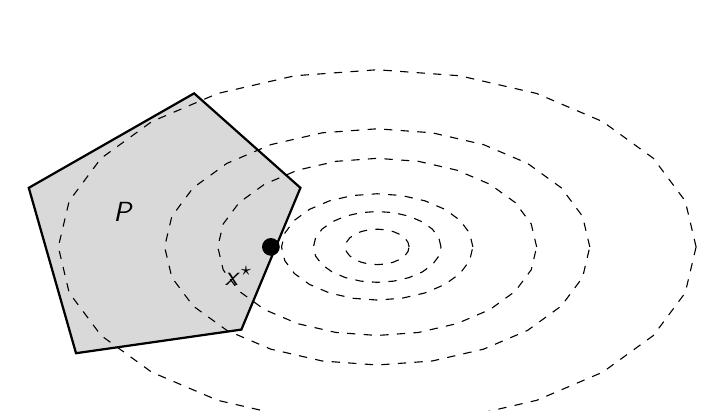
\begin{tikzpicture}[scale=1.5]
		
		% Polytope
		\fill[gray!30]
		(0,0) -- (1.4,0.2) -- (1.9,1.4) -- (1.0,2.2) -- (-0.4,1.4) -- cycle;
		\draw[black, thick]
		(0,0) -- (1.4,0.2) -- (1.9,1.4) -- (1.0,2.2) -- (-0.4,1.4) -- cycle;
		
		% Quadratic contours (elliptical shapes)
		\foreach \scale in {0.6,1.2,1.8,3,4,6} {
			\draw[dashed, domain=0:360]
			plot ({2.55 + 0.45*\scale*cos(\x)}, {0.9 + 0.25*\scale*sin(\x)});
		}
		
		% Optimal point
		\filldraw[black] (1.65,0.9) circle (2pt);
		\node at (1.38,0.65) {$x^\star$};
		
		% Label inside polytope
		\node at (0.4,1.2) {$P$};
		
	\end{tikzpicture}
	\caption{Convex quadratic optimisation on a polytope. Contours indicate
		decreasing objective value towards the optimal point $x^\star$.}
	\label{fig:QP}
\end{figure}

Convex QPs benefit from strong theoretical guarantees and can be solved
efficiently using interior-point, active-set, or first-order optimisation
methods. They are widely used in control, signal processing, finance,
estimation, and engineering design.

\begin{examplebox}{Example: Robot Distance to a Restricted Zone}
	\textbf{Scenario:} Let a robot is located at coordinates $p = (3, 2)$. A restricted geometric zone $\mathcal{X}$ (representing an obstacle or a target landing pad) is defined as a unit box centered at the origin. The robot must compute the shortest distance to this zone to plan its trajectory.
	
	\solution
	
	\textbf{Optimisation Problem:}
	Find the point $x \in \mathcal{X}$ closest to $p$:
	\begin{equation*}
		\min_{x \in \mathbb{R}^2} \; (x_1 - 3)^2 + (x_2 - 2)^2
	\end{equation*}
	
	\textbf{Constraints (Standard Format):}
	The unit box is defined by bounds $-1 \leq x_1 \leq 1$ and $-1 \leq x_2 \leq 1$. In standard linear inequality form $Ax \leq b$, these are written as:
	\begin{align*}
		x_1 &\leq 1 \\
		-x_1 &\leq 1 \\
		x_2 &\leq 1 \\
		-x_2 &\leq 1
	\end{align*}
	
	\textbf{Visualising the Solution:}
	By inspecting the geometry (see Figure \ref{fig:qp_distance}), the closest point within the box to $(3,2)$ is the upper-right corner of the box, $x^* = (1, 1)$.
	
	\begin{center}
		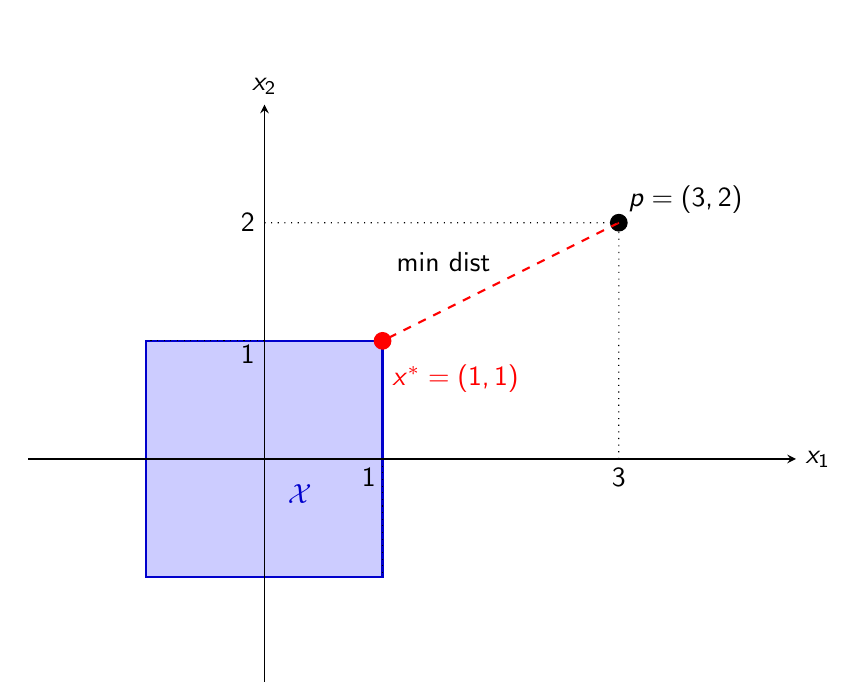
\begin{tikzpicture}[scale=1.5, >=stealth]
			% Draw Axes
			
			
			% Draw the Box (Constraint Set X)
			% Fill with light blue, thick border
			\filldraw[fill=blue!20, draw=blue!80!black, thick] (-1, -1) rectangle (1, 1);
			\node[blue!80!black] at (0.3, -0.3) {$\mathcal{X}$};
			
			% Draw the Robot/Target Point p
			\coordinate (P) at (3, 2);
			\filldraw[black] (P) circle (2pt) node[above right] {$p = (3, 2)$};
			
			% Draw the Solution Point x*
			\coordinate (Sol) at (1, 1);
			\filldraw[red] (Sol) circle (2pt) node[below right, yshift=-5pt] {$x^* = (1, 1)$};
			
			% Draw the distance line
			\draw[red, dashed, thick] (P) -- (Sol) node[midway, above left, text=black] {min dist};
			
			% Draw projection lines for the Point P
			\draw[dotted] (3, 0) node[below] {$3$} -- (P);
			\draw[dotted] (0, 2) node[left] {$2$} -- (P);
			
			% Draw projection lines for the Box limits
			\draw[dotted] (1, 0) node[below, xshift=-5pt] {$1$} -- (1, -1);
			\draw[dotted] (0, 1) node[left, yshift=-5pt] {$1$} -- (-1, 1);
			
			\draw[->] (-2, 0) -- (4.5, 0) node[right] {$x_1$};
			\draw[->] (0, -2) -- (0, 3) node[above] {$x_2$};
			
		\end{tikzpicture}
		\captionof{figure}{Geometry of the optimisation problem.}
		\label{fig:qp_distance}
	\end{center}
	
	To solve this problem numerically using a solver (like OSQP, quadprog, or GUROBI), we must map the problem into the standard Quadratic Programming form:
	\begin{equation}
		\min_{x} \; \frac{1}{2} x^\top P x + q^\top x \quad \text{subject to} \quad Gx \leq h
	\end{equation}
	
	
	We expand the squared Euclidean distance objective:
	\begin{align*}
		J(x) &= (x_1 - 3)^2 + (x_2 - 2)^2 \\
		&= (x_1^2 - 6x_1 + 9) + (x_2^2 - 4x_2 + 4) \\
		&= \underbrace{x_1^2 + x_2^2}_{\text{Quadratic part}} \underbrace{- 6x_1 - 4x_2}_{\text{Linear part}} + \underbrace{13}_{\text{Constant}}
	\end{align*}
	The constant term ($13$) does not affect the optimal location $x^*$ and is discarded. To match the standard form $\frac{1}{2} x^\top P x$, the matrix $P$ must be scaled such that the diagonal elements are 2.
	\[
	\frac{1}{2} \underbrace{\begin{bmatrix} x_1 & x_2 \end{bmatrix}}_{x^\top}
	\underbrace{\begin{bmatrix} 2 & 0 \\ 0 & 2 \end{bmatrix}}_{P} 
	\underbrace{\begin{bmatrix} x_1 \\ x_2 \end{bmatrix}}_{x}
	+ 
	\underbrace{\begin{bmatrix} -6 & -4 \end{bmatrix}}_{q^\top} 
	\begin{bmatrix} x_1 \\ x_2 \end{bmatrix}
	\]
	Thus, we define:
	\[
	P = \begin{bmatrix} 2 & 0 \\ 0 & 2 \end{bmatrix}, \quad 
	q = \begin{bmatrix} -6 \\ -4 \end{bmatrix}
	\]
	
	
	The unit box constraints are:
	\[
	-1 \leq x_1 \leq 1 \quad \text{and} \quad -1 \leq x_2 \leq 1
	\]
	These must be rewritten as "less than or equal to" inequalities ($Gx \leq h$):
	\begin{align*}
		x_1 &\leq 1 \\
		-x_1 &\leq 1 \\
		x_2 &\leq 1 \\
		-x_2 &\leq 1 
	\end{align*}
	In matrix notation, this becomes:
	\[
	\underbrace{\begin{bmatrix} 
			1 &  0 \\
			-1 &  0 \\
			0 &  1 \\
			0 & -1 
	\end{bmatrix}}_{G} 
	\begin{bmatrix} x_1 \\ x_2 \end{bmatrix} 
	\leq 
	\underbrace{\begin{bmatrix} 
			1 \\ 1 \\ 1 \\ 1 
	\end{bmatrix}}_{h}
	\]	

\subsection*{MATLAB Implementation using YALMIP}
Having derived the standard QP matrices manually, we can now solve the problem using MATLAB. The following code demonstrates YALMIP's symbolic framework to automate the process.

\begin{lstlisting}[caption={Solving the Robot Trajectory QP using YALMIP and quadprog.}, label={lst:yalmip_qp}]
	clear; clc;
	ops = sdpsettings('solver', 'quadprog', 'verbose', 0);
	
	p = [3; 2];          % Robot position
	x = sdpvar(2, 1);    % Variable
	
	Objective  = (x(1) - p(1))^2 + (x(2) - p(2))^2;
	
	Constraints = [-1 <= x <= 1];
	
	optimize(Constraints , Objective, ops);
	
	x_opt = value(x);
	fprintf('Optimal Sol : x1=%.2f, x2=%.2f\n', x_opt(1), x_opt(2));
\end{lstlisting}	

\subsection*{Direct Implementation using quadprog}
While YALMIP offers a convenient high-level interface, it is essential to understand how to pass the problem matrices directly to a solver. This effectively opens the "black box" of the optimisation tool.

In MATLAB, the native solver \texttt{quadprog}\footnote{requires optimization toolbox} solves problems of the form:
\begin{equation*}
	\min_x \frac{1}{2}x^\top H x + f^\top x \quad \text{subject to} \quad A x \leq b
\end{equation*}
This syntax requires a direct mapping from our mathematical notation ($P, q, G, h$) to MATLAB's standard arguments ($H, f, A, b$).

\begin{lstlisting}[caption={Direct solution using MATLAB's built-in quadprog solver.}, label={lst:quadprog_direct}]
	clear; clc;
	
	% 1. Map the Mathematical Notation to MATLAB Syntax
	% Objective: 1/2 * x'*P*x + q'*x
	H = [2, 0; 
			0, 2];         	% Our Matrix P
	f = [-6; -4];       % Our Vector q
	
	% Constraints: G*x <= h
	A = [ 1,  0; 
			-1,  0; 
			0,  1; 
			0, -1];       % Our Matrix G
	b = [1; 1; 1; 1];   % Our Vector h
	
	% 2. Set Options (optional, to suppress command window output)
	options = optimoptions('quadprog', 'Display', 'off');
	
	% 3. Call the Solver
	% Syntax: x = quadprog(H, f, A, b)
	x_opt = quadprog(H, f, A, b, [], [], [], [], [], options);
	
	% 4. Display Results
	fprintf('Optimal Sol : x1=%.2f, x2=%.2f\n', x_opt(1), x_opt(2));
\end{lstlisting}
	
\end{examplebox}





% --------------------------------------------------------
\subsubsection{Nonconvex Quadratic Programmes}

Not all optimisation problems retain convexity. Once convexity is lost, global optimality becomes substantially harder to guarantee. While standard MPC relies on convex optimisation, certain control formulations lead to nonconvex problems. A specific class of these "hard" problems is the Nonconvex Quadratic Programme (QP).

When the matrix $P$ in the quadratic objective is not positive semidefinite ($P \not\succeq 0$), the objective function is nonconvex. This often manifests as saddle-shaped level sets. Consequently, the feasible polytope may contain multiple local minima, making the global optimum difficult to find efficiently.

The formulation is given by:
\begin{align*}
	&\min_x \quad \frac{1}{2} x^{\top} Px + q^{\top} x\\
	 \text{subject to: }& \\
	&Gx \le h \\
	& Ax = b 
\end{align*}

\begin{figure}[h]
	\centering
	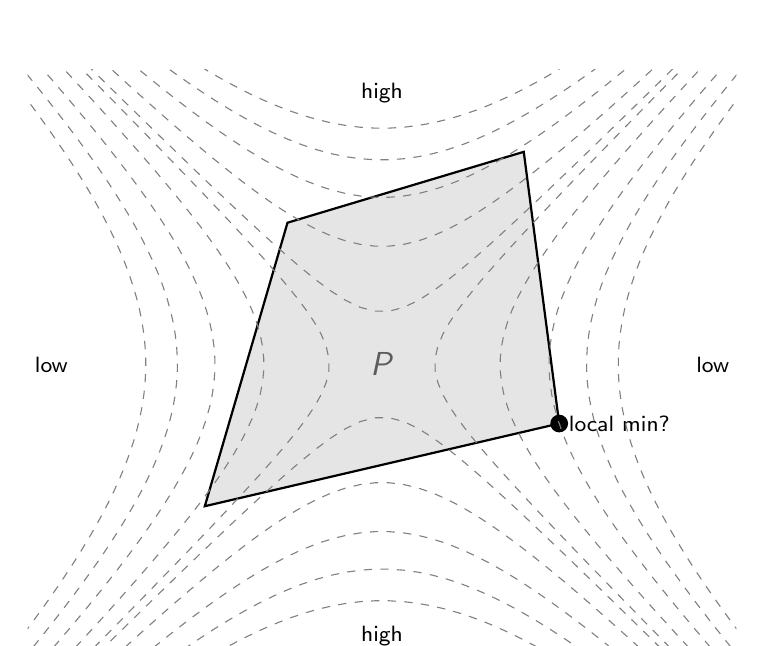
\begin{tikzpicture}[scale=1.5]
		% Clip everything to a reasonable viewing box
		\clip (-3,-2.5) rectangle (3,2.5);
		
		% 2. Draw the Polytope (Feasible Set)
		% Arbitrary shape crossing the saddle
		\coordinate (P1) at (-1.5, -1.2);
		\coordinate (P2) at (1.5, -0.5);
		\coordinate (P3) at (1.2, 1.8);
		\coordinate (P4) at (-0.8, 1.2);
		
		\fill[gray!40, opacity=0.5] (P1) -- (P2) -- (P3) -- (P4) -- cycle;
		\draw[thick, black] (P1) -- (P2) -- (P3) -- (P4) -- cycle;
		
		% 3. Annotations
		\node at (0,0) [font=\large, opacity=0.6] {$P$};
		
		% Labels matching the visual style of the slide
		\node[font=\footnotesize, fill=white, inner sep=1pt] at (0, 2.3) {high};
		\node[font=\footnotesize, fill=white, inner sep=1pt] at (0, -2.3) {high};
		\node[font=\footnotesize, fill=white, inner sep=1pt] at (-2.8, 0) {low};
		\node[font=\footnotesize, fill=white, inner sep=1pt] at (2.8, 0) {low};
		
		% Example stationary point / vertex
		\filldraw (P2) circle (2pt); 
		\node[right, font=\footnotesize] at (P2) {local min?};
		
		% Vertical Hyperbolas (Opening Up/Down)
		% y = +/- sqrt(x^2 - c) for c < 0 (or x^2 - y^2 = -k)
		\foreach \k in {0.2, 1, 2, 3, 4} {
			\draw[dashed, gray] plot[domain=-3:3, samples=50] (\x, {sqrt(\x*\x + \k)});
			\draw[dashed, gray] plot[domain=-3:3, samples=50] (\x, {-sqrt(\x*\x + \k)});
		}
		
		% Horizontal Hyperbolas (Opening Left/Right)
		% x = +/- sqrt(y^2 + k) 
		% We use \x as the parameter for the vertical axis (y-value) here
		\foreach \k in {0.2, 1, 2, 3, 4} {
			\draw[dashed, gray] plot[domain=-2.5:2.5, samples=50] ({sqrt(\x*\x + \k)}, \x);
			\draw[dashed, gray] plot[domain=-2.5:2.5, samples=50] ({-sqrt(\x*\x + \k)}, \x);
		}
		
	\end{tikzpicture}
	\caption{Nonconvex quadratic optimisation on a polytope. The dashed lines represent the contours of a saddle-shaped objective function. The global optimum is likely at a vertex, but local minima may exist.}
	\label{fig:NonconvexQP}
\end{figure}

% --------------------------------------------------------
\subsubsection{Mixed-Integer Linear Programmes (MILPs)}

A Mixed-Integer Linear Programme retains the linear objective and constraints of an LP but imposes integrality restrictions on some or all decision variables:
\begin{align*}
	&\min_{x} \quad c^{\top} x \\
	 \text{subject to: } & \\
	&Gx \le h \\
	&Ax = b \\
	&x \in \{0,1\}^n \;\; \text{or} \;\; x \in \mathbb{Z}^n .
\end{align*}

The feasible set becomes a set of discrete points embedded within a polyhedron, leading to a combinatorial explosion in complexity. Figure~\ref{fig:MIP} shows a sketch of a possible mixed-integer problem. 

\begin{examplebox}{MILP: Industrial Energy Management}
	
	\textbf{The General Problem:}
	Consider an industrial site supplied by the electrical grid and equipped with a dispatchable generator and a battery energy storage system. The objective is to minimise the total operating cost over a finite horizon of $N$ discrete time steps of duration $\Delta t$, while meeting the site demand and respecting operational constraints.
	
	The generator can be switched on or off and incurs both fuel and start-up costs. The battery is subject to energy dynamics and cannot charge and discharge simultaneously.
	
	\medskip
	
	For each time step $k=1,\dots,N$, define:
	\begin{align*}
		p_g(k) &\ge 0 && \text{generator power (kW)},\\
		p_{\mathrm{grid}}(k) &\ge 0 && \text{grid import power (kW)},\\
		p_{\mathrm{ch}}(k),\, p_{\mathrm{dis}}(k) &\ge 0 && \text{battery charge/discharge power (kW)},\\
		E(k) & && \text{battery energy (kWh)},\\
		u(k) &\in \{0,1\} && \text{generator on/off status},\\
		s(k) &\in \{0,1\} && \text{generator start-up indicator},\\
		z(k) &\in \{0,1\} && \text{battery charge mode indicator}.
	\end{align*}
	
	\medskip
	\textbf{Objective function:}
	The total operating cost is given by
	\begin{equation}
		\min \sum_{k=1}^{N} \Delta t 
		\left(
		c_{\mathrm{grid}}(k)\,p_{\mathrm{grid}}(k)
		+
		c_f\,p_g(k)
		\right)
		+
		\sum_{k=1}^{N} c_{\mathrm{start}}\, s(k),
	\end{equation}
	where $c_{\mathrm{grid}}(k)$ denotes the time-varying electricity price, $c_f$ the generator fuel cost coefficient, and $c_{\mathrm{start}}$ the generator start-up cost.
	
	\medskip
	\textbf{Constraints:}
	
	\emph{Power balance:}
	\begin{equation}
		p_{\mathrm{grid}}(k) + p_g(k) + p_{\mathrm{dis}}(k) - p_{\mathrm{ch}}(k) = d(k),
		\quad \forall k.
	\end{equation}
	The term $d(k)$ represents the exogenous electrical demand (load) of the system at time step $k$, assumed to be known over the prediction horizon.
	
	\emph{Generator operating limits:}
	\begin{equation}
		P_{g,\min} u(k) \le p_g(k) \le P_{g,\max} u(k),
		\quad \forall k.
	\end{equation}
	
	\emph{Generator start-up logic:}
	\begin{align}
		s(1) &\ge u(1),\\
		s(k) &\ge u(k) - u(k-1), \quad k=2,\dots,N.
	\end{align}
	where $s(k)$ is a binary variable that equals one if the generator is started at time $k$, i.e. when the on/off status $u(k)$ transitions from 0 to 1.
	
	\emph{Battery energy dynamics:}
	\begin{equation}
		E(k+1) = E(k) + \Delta t\,\eta_{\mathrm{ch}}\,p_{\mathrm{ch}}(k)
		- \Delta t\,\frac{1}{\eta_{\mathrm{dis}}}\,p_{\mathrm{dis}}(k),
	\end{equation}
	with $E(1)=E_0$. Also, $\eta_{\mathrm{ch}}\in(0,1]$ and $\eta_{\mathrm{dis}}\in(0,1]$ denote the charging and discharging efficiencies of the battery, respectively.
	
	\emph{Battery and grid limits:}
	\begin{align}
		E_{\min} &\le E(k) \le E_{\max},\\
		0 &\le p_{\mathrm{ch}}(k) \le P_{\mathrm{ch},\max},\\
		0 &\le p_{\mathrm{dis}}(k) \le P_{\mathrm{dis},\max},\\
		0 &\le p_{\mathrm{grid}}(k) \le P_{\mathrm{grid},\max}.
	\end{align}
	
	\emph{Nonsimultaneous charging and discharging:}
	\begin{align}
		p_{\mathrm{ch}}(k) &\le P_{\mathrm{ch},\max} z(k),\\
		p_{\mathrm{dis}}(k) &\le P_{\mathrm{dis},\max} [1-z(k)].
	\end{align}
	
	\tcbline
	\textbf{Solving this problem:}
	The model above is a Mixed-Integer Linear Programme (MILP) due to the binary variables $u(k), s(k), z(k)$. It requires specialised solvers like Gurobi or CPLEX. In the software section later, we will implement a \textbf{simplified} version of this (a continuous LP) to demonstrate the concept in MATLAB.
	
\end{examplebox}


\begin{figure}[!htb]
	\centering
	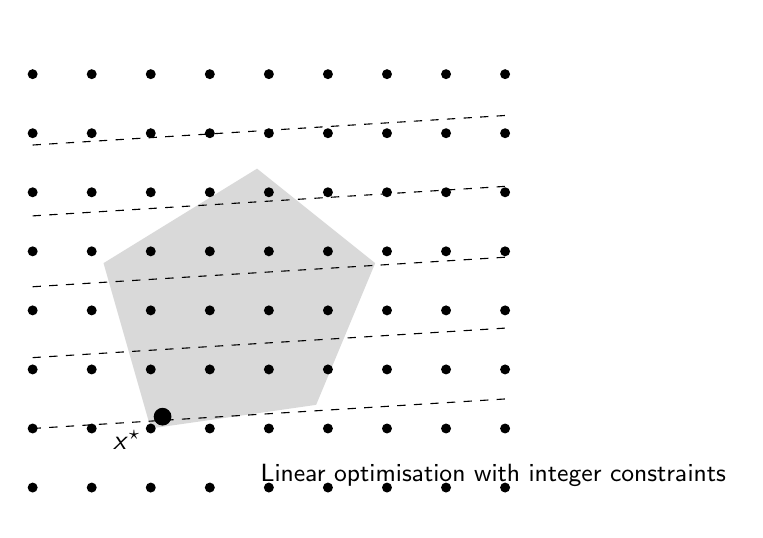
\begin{tikzpicture}[scale=1.5]
		
		% Polytope
		\fill[gray!30]
		(0,0) -- (1.4,0.2) -- (1.9,1.4) -- (0.9,2.2) -- (-0.4,1.4) -- cycle;
		
		% Grid of integer points
		\foreach \x in {-1,-0.5,...,3} {
			\foreach \y in {-1,-0.5,...,3} {
				\fill (\x,\y) circle (1.2pt);
			}
		}
		
		% Parallel cost hyperplanes
		\foreach \y in {0.0,0.6,1.2,1.8,2.4} {
			\draw[dashed] (-1,\y) -- (3,\y+0.25);
		}
		
		% Integer-optimal point
		\filldraw[black] (0.1,0.1) circle (2pt);
		\node at (-0.2,-0.1) {$x^\star$};
		
		\node at (2.9,-0.4) {\small Linear optimisation with integer constraints};
		
	\end{tikzpicture}
	\caption{MILP feasible set: discrete integer lattice points within a polytope.}
	\label{fig:MIP}
\end{figure}

\section{Software Tools for Optimisation}

Implementing Model Predictive Control (MPC) requires a robust software stack. Generally, the implementation workflow is divided into two distinct layers:
\begin{enumerate}
	\item \textbf{Parsers (Modelling Languages):} High-level interfaces that allow the user to define the optimisation problem using intuitive algebraic syntax (e.g., \texttt{x\^{}2 + y\^{}2 <= 1}). The parser translates this symbolic representation into the standard numerical matrix formats required by the solver.
	\item \textbf{Solvers:} The low-level numerical engines that perform the mathematical iterations to find the optimal solution (e.g., Active-Set methods or Interior-Point methods).
\end{enumerate}

\subsection{Modelling Languages (Parsers)}

Choosing the right parser depends heavily on the programming environment (MATLAB vs. Python) and the type of problem (Convex vs. Nonlinear).

For \textbf{MATLAB} users, \textbf{YALMIP} is the de facto standard for prototyping. It supports a vast array of solvers and allows users to switch between them by changing a single line of code. \textbf{CVX} is another popular option, specifically designed for Disciplined Convex Programming (DCP), a methodology that requires users to compose their optimisation problems from a fixed library of convex functions and composition rules so that convexity is automatically verified.

For \textbf{Python} users, \textbf{CVXPY} is the equivalent of CVX, providing a clean object-oriented interface for convex problems. 

For \textbf{Nonlinear MPC (NMPC)} and high-performance applications, \textbf{CasADi} is widely used in both Python and MATLAB. Unlike standard parsers, CasADi implements Algorithmic Differentiation (AD), allowing it to compute exact gradients and Hessians automatically, which is critical for solving nonlinear control problems efficiently.

\begin{table}[h]
	\centering
	\caption{Comparison of Common Modelling Languages (Parsers)}
	\label{tab:parsers}
	\renewcommand{\arraystretch}{1.3}
	\begin{tabularx}{\textwidth}{@{}l l l X@{}}
		\toprule
		\textbf{Name} & \textbf{Platform} & \textbf{License} & \textbf{Primary Purpose \& Notes} \\
		\midrule
		\textbf{YALMIP} & MATLAB & Free & The \emph{Swiss Army Knife} of MATLAB optimisation. Excellent for prototyping QP, LP, SDP, and MIP. \\
		\textbf{CVX} & MATLAB & Free & Enforces Disciplined Convex Programming (DCP). Guarantees convexity but stricter than YALMIP. \\
		\textbf{CVXPY} & Python & Free (Apache) & The standard for convex optimisation in Python. Intuitive object-oriented syntax. \\
		\textbf{CasADi} & Python/C++ & Free (LGPL) & Ideal for Nonlinear MPC (NMPC). Features algorithmic differentiation and C-code generation for embedded targets. \\
		\textbf{Pyomo} & Python & Free (BSD) & General modelling language, widely used in Operations Research (OR) and process systems engineering. \\
		\textbf{JuMP} & Julia & Free (MIT) & Extremely fast modelling language. Gaining significant popularity in the control community. \\
		\bottomrule
	\end{tabularx}
\end{table}

\subsection{Numerical Solvers}

The choice of solver is dictated by the problem class and the deployment requirements.

\subsubsection*{Linear and Quadratic Solvers (Standard MPC)}
For linear MPC, we typically solve a \textbf{Quadratic Programme (QP)}. Solvers like \textbf{OSQP} (Operator Splitting Quadratic Programme) and \textbf{quadprog} are popular because they are robust, code-generatable, and solve for moderate accuracy very quickly. \textbf{qpOASES} is an active-set solver specifically designed for MPC; it uses "warm-starting" to solve the next time-step's problem almost instantly based on the previous solution.

For commercial applications, \textbf{Gurobi} and \textbf{CPLEX} are the industry leaders, offering unmatched speed for large-scale Mixed-Integer (MIP) and convex problems.

\subsubsection*{Conic and Nonlinear Solvers (Robust \& Nonlinear MPC)}
If the MPC formulation involves ellipsoidal constraints (Robust MPC) or Linear Matrix Inequalities (LMIs), a \textbf{Conic Solver} is required. \textbf{MOSEK} is the industry leader for these types of problems (SOCP and SDP). For pure MATLAB-based research involving LMIs, \textbf{SeDuMi} remains a classic open-source option.

For Nonlinear MPC, \textbf{IPOPT} (Interior Point OPTimizer) is the standard open-source engine, often paired with CasADi.

\begin{table}[h]
	\centering
	\caption{List of Common Numerical Solvers}
	\label{tab:solvers}
	\renewcommand{\arraystretch}{1.3}
	\begin{tabularx}{\textwidth}{@{}l l l l X@{}}
		\toprule
		\textbf{Solver} & \textbf{Type} & \textbf{Method} & \textbf{License} & \textbf{Best For} \\
		\midrule
		\textbf{quadprog} & QP & Interior-Point & Proprietary & Standard MATLAB solver (requires Opt. Toolbox). {Primary solver used in this course}. \\
		\textbf{OSQP} & QP & ADMM\footnote{ADMM (Alternating Direction Method of Multipliers) is a first-order algorithm that decomposes a large optimisation problem into smaller sub-problems that are solved in alternation, making it well suited to embedded and real-time applications.} & Free (Apache) & Embedded MPC. Very robust, division-free code; widely used in Python/Julia. \\
		\textbf{qpOASES} & QP & Active-Set & Free (LGPL) & Small-to-medium MPC. Excellent {warm-starting} capabilities for dense problems. \\
		\textbf{Gurobi} & LP, QP, MIP & Simplex/Barrier & Commercial & Gold standard for MIP and convex speed. Free academic licenses available. \\
		\textbf{MOSEK} & SOCP, SDP & Interior-Point & Commercial & The leader for {Robust MPC} (Conic constraints) and Semidefinite programming. \\
		\textbf{SeDuMi} & SDP, SOCP & Interior-Point & Free (GPL) & Established MATLAB solver for Linear Matrix Inequality(LMI)-based control and stability analysis. \\
		\textbf{IPOPT} & NLP & Interior-Point & Free (EPL) & Large-scale nonlinear optimisation (NMPC). Standard engine for CasADi. \\
		\textbf{SNOPT} & NLP & SQP & Commercial & Highly nonlinear, non-convex problems (e.g., aerospace trajectory planning). \\
		\textbf{ECOS} & SOCP, LP & Interior-Point & Free (GPL) & Lightweight, embedded-friendly Second-Order Cone solver. \\
		\bottomrule
	\end{tabularx}
\end{table}



\section{Solving Optimisation Problems: From Theory to Code}

Mathematical formulation is only half the battle. To deploy Model Predictive Control, we must translate these equations into code that a computer can solve. In this section, we explore a complex energy management system as an example.


\subsection{Economic MPC for Smart Grids}

In this  example, we explore a sophisticated application of optimisation: \textbf{Economic Energy Management}.  The goal here is purely economic: minimise the total cost of electricity over a 24-hour horizon.

\subsubsection{Problem Scenario}
Although the general problem formulation (the MILP discussed earlier) included complex generator logic, for this MATLAB example we will solve a simplified but highly relevant subset: {Battery Energy Arbitrage}.

Consider a home with:
\begin{itemize}
	\item \textbf{Load ($P_{load}$):} The household power consumption (lighting, appliances).
	\item \textbf{Solar Generation ($P_{solar}$):} Free renewable energy available during the day.
	\item \textbf{Battery Storage:} A unit capable of storing energy ($E_{bat}$) to bridge the gap between supply and demand.
	\item \textbf{Grid Connection:} Allows buying power when needed or selling excess power.
\end{itemize}

\textbf{The Challenge:} Electricity prices fluctuate throughout the day (Time-of-Use pricing). Prices are low at night and high in the evening. We must decide the optimal battery charge/discharge schedule to minimise the daily bill.

\subsubsection{Mathematical Formulation}
We define the discrete time step $\Delta t = 1$ hour and the horizon $N=24$ hours.

\textbf{1. Variables:}
\begin{itemize}
	\item $P_{grid}(k)$: Power exchanged with the grid (kW). Positive = Buy, Negative = Sell.
	\item $P_{bat}(k)$: Battery charging power (kW). Positive = Charge, Negative = Discharge.
	\item $E_{bat}(k)$: Energy stored in the battery (kWh).
\end{itemize}

\textbf{2. The Objective Function:}
Minimise the cumulative cost of grid usage:
\begin{equation}
	\min_{P_{bat}, P_{grid}} \sum_{k=0}^{N-1} \text{Price}(k) \times P_{grid}(k) \cdot \Delta t
\end{equation}

\textbf{3. Constraints:}
\begin{align}
	\text{Power Balance:} \quad & P_{grid}(k) + P_{solar}(k) = P_{load}(k) + P_{bat}(k) \\
	\text{Dynamics:} \quad & E_{bat}(k+1) = E_{bat}(k) + P_{bat}(k) \cdot \Delta t \\
	\text{Capacity Limits:} \quad & E_{min} \leq E_{bat}(k) \leq E_{max} \\
	\text{Power Limits:} \quad & P_{min} \leq P_{bat}(k) \leq P_{max}
\end{align}

\subsubsection{Implementation (MATLAB \& YALMIP)}
We use YALMIP to translate this word problem into a numerical format. Since this problem is purely continuous, we solve it as a Linear Programme (LP) using \texttt{quadprog} (with zero quadratic cost) or \texttt{linprog}.

\begin{lstlisting}[language=Matlab]
	% --- 1. System Parameters ---
	N = 24;                 % Horizon (24 hours)
	E_cap = 13.5;           % Battery Capacity (kWh, e.g., Tesla Powerwall)
	P_max = 5;              % Max Charge/Discharge rate (kW)
	dt = 1;                 % Time step (1 hour)
	
	% --- 2. Forecast Data (Profiles) ---
	% Price: 0.10 (Off-peak), 0.30 (Peak: 17:00-21:00)
	Price = 0.10 * ones(N,1);  Price(18:21) = 0.30; 
	
	% Solar: Peak at noon (simple sine wave approx)
	t = (0:N-1)';
	Solar = max(0, 4 * sin(pi * (t - 6) / 12)); 
	
	% Load: Peaks in morning and evening
	Load = 1 + 2 * exp(-(t-19).^2/10) + 1 * exp(-(t-8).^2/5);
	
	% --- 3. Optimisation Variables ---
	P_grid = sdpvar(N, 1);   % Grid Power
	P_bat  = sdpvar(N, 1);   % Battery Power
	E_bat  = sdpvar(N+1, 1); % Battery State of Charge
	
	% --- 4. Constraints Construction ---
	C = [];
	
	% Start with empty battery (Assumption for this specific day)
	% In real MPC, E_bat(1) would equal the measured sensor value.
	C = [C, E_bat(1) == 0]; 
	
	for k = 1:N
		% Dynamics: Energy integration
		C = [C, E_bat(k+1) == E_bat(k) + P_bat(k) * dt];
	
		% Power Balance: Supply (Grid+Solar) = Demand (Load+BatteryCharge)
		C = [C, P_grid(k) + Solar(k) == Load(k) + P_bat(k)];
	
		% Physical Constraints
		C = [C, 0 <= E_bat(k+1) <= E_cap]; % Capacity limits
		C = [C, -P_max <= P_bat(k) <= P_max]; % Power limits
	end
	
	% --- 5. Objective: Minimise Total Cost ---
	Objective = Price' * P_grid;
	
	% --- 6. Solve ---
	ops = sdpsettings('solver','quadprog','verbose',0);
	sol = optimize(C, Objective, ops);
\end{lstlisting}


\subsubsection{Visualising the Result}

The result is best understood visually (Figure \ref{fig:smartgrid}). 
\begin{enumerate}
	\item \textbf{Pre-Charging:} Notice that between 00:00 and 06:00, the battery charges (blue bars positive) even though the sun isn't shining. It buys cheap electricity to store it.
	\item \textbf{Peak Shaving:} During the peak price window (17:00--21:00), the battery discharges (blue bars negative). The optimiser "decided" to sell the stored energy to avoid paying the high grid price, drastically reducing the bill.
\end{enumerate}

\begin{figure}[!htb]
	\centering
	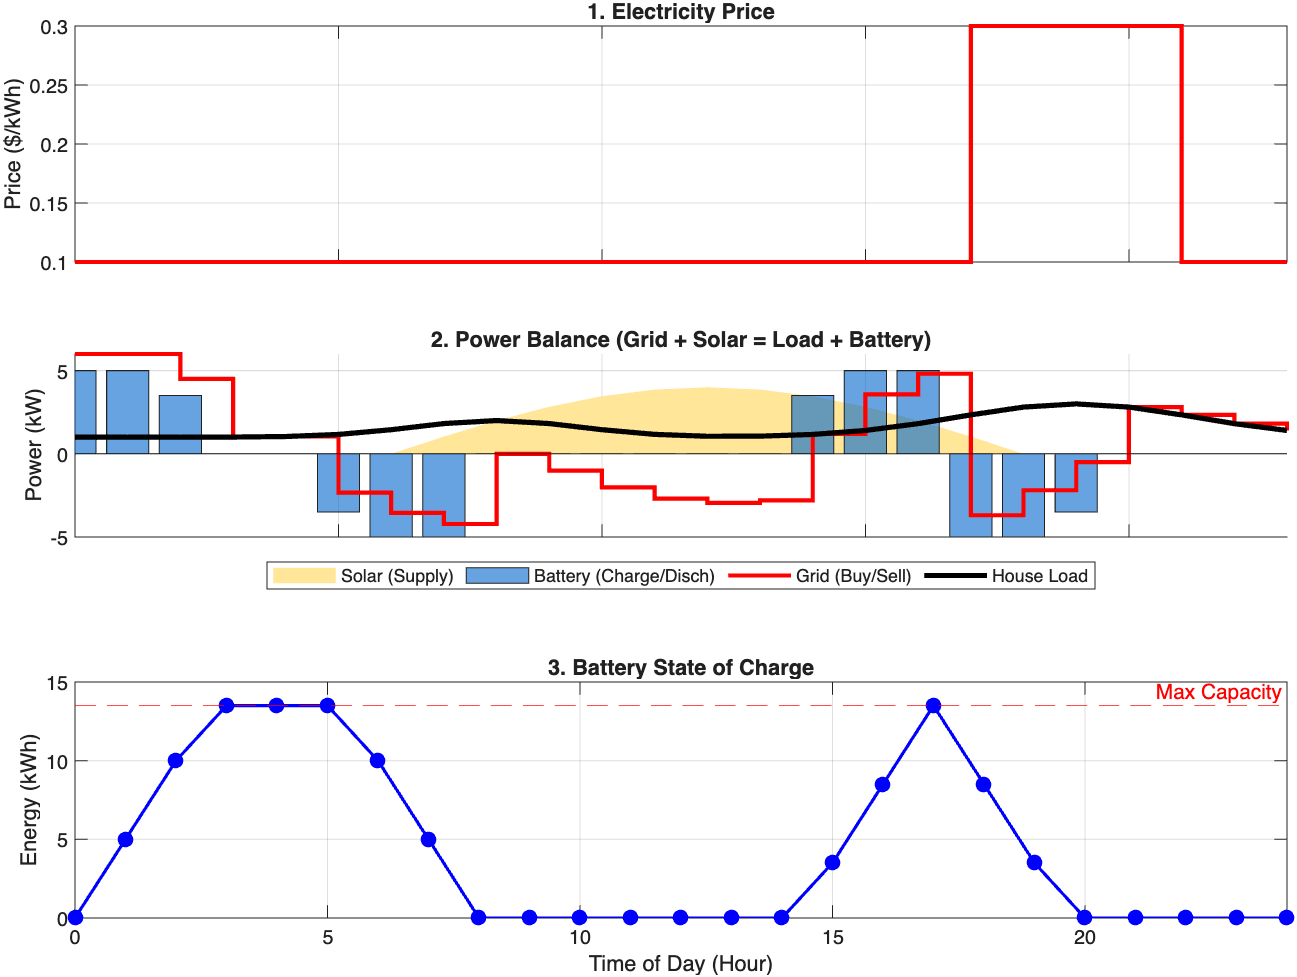
\includegraphics[width=1\linewidth]{Figures/energy_management}
	\caption{\textbf{Economic Optimisation Results.} \textbf{Top:} The Time-of-Use price signal with a peak period between hours 17:00 and 21:00. \textbf{Middle:} Visual verification of the power balance equation ($P_{grid} + P_{solar} = P_{load} + P_{bat}$). Note the \textbf{Grid usage (Red line)}: the system buys power at night to pre-charge the battery (positive red step) and sells power back to the grid during the peak price window (negative red step), effectively performing energy arbitrage. \textbf{Bottom:} The state of charge trajectory, showing the battery filling up in anticipation of the price spike and emptying completely to maximise revenue.}
	\label{fig:smartgrid}
\end{figure}

\section{Key Takeaways}
\begin{itemize}
	\item \textbf{Optimisation is Translation:} MPC translates qualitative engineering goals (e.g., ``drive fast but don't crash'') into quantitative mathematical statements (e.g., ``minimise travel time subject to velocity limits'').
\item \textbf{The Scalar Score:} An algorithm cannot minimise a vector or a list of conflicting goals. The \emph{objective function} $J(x)$ serves to compress complex multi-variable decisions into a single scalar number (a cost), allowing different control strategies to be ranked and compared.

\item \textbf{Constraints Define Reality:} Unlike classical control, where saturation is often an afterthought, optimisation explicitly handles physical limitations. The \emph{feasible set} is the intersection of all equality and inequality constraints. If this set is empty, the problem is infeasible, and no solution exists.

\item \textbf{Convexity:} The most critical property of an optimisation problem is convexity. If the objective function is convex (bowl-shaped) and the constraints form a convex set, any local minimum found is guaranteed to be the \textbf{global minimum}. This reliability is essential for safety-critical control systems.

\item \textbf{Standard Forms:}
\begin{itemize}
	\item \textbf{LP (Linear Programme):} Linear cost and constraints. extremely fast; used for economic dispatch and simple regulation.
	\item \textbf{QP (Quadratic Programme):} Quadratic cost (energy/error) and linear constraints. This is the standard formulation for linear MPC.
	\item \textbf{MILP (Mixed-Integer):} Contains discrete decisions (On/Off). Computationally expensive but necessary for logic-based control.
\end{itemize}

\item \textbf{Minimisation vs. Maximisation:} Solvers generally seek to minimise cost. To maximise a benefit (like profit), we simply minimise the negative of that function:
\[ \arg \max f(x) \equiv \arg \min (-f(x)) \]
\end{itemize}

\section*{Exercises}
\begin{enumerate}
	\item \textbf{Convex Sets and Functions.}
	Determine whether each of the following sets is convex. Justify your answer using the definition $\lambda x + (1-\lambda)y \in \mathcal{X}$ for all $\lambda \in [0,1]$ and all $x, y \in \mathcal{X}$.
	\begin{enumerate}
		\item $\mathcal{X}_1 = \{x \in \mathbb{R}^2 \mid x_1^2 + x_2^2 \leq 4\}$
		\item $\mathcal{X}_2 = \{x \in \mathbb{R}^2 \mid x_1^2 + x_2^2 \geq 1\}$
		\item $\mathcal{X}_3 = \{x \in \mathbb{R}^2 \mid 2x_1 + 3x_2 \leq 6, \ x_1 \geq 0, \ x_2 \geq 0\}$
	\end{enumerate}
	Furthermore, determine whether $f(x) = 5x_1^2 - 4x_1 x_2 + 3x_2^2$ is convex by computing its Hessian and checking the eigenvalues.

	\item \textbf{Gradient and Hessian Computation.}
	Consider the function
	\[
	J(x) = 4x_1^2 + 6x_1 x_2 + 8x_2^2 - 10x_1 + 2x_2.
	\]
	\begin{enumerate}
		\item Compute the gradient $\nabla J(x)$ and find the stationary point by solving $\nabla J(x) = 0$.
		\item Compute the Hessian matrix $H = \nabla^2 J(x)$.
		\item Determine whether $H$ is positive definite, positive semidefinite, or indefinite. What does this imply about the stationary point found in~(a)?
	\end{enumerate}

	\item \textbf{Optimality Conditions for Equality-Constrained Problems.}
	Consider the problem
	\begin{equation*}
		\begin{aligned}
			\min_{x \in \mathbb{R}^2} \quad & J(x) = x_1^2 + x_2^2 \\
			\text{s.t.} \quad & h(x) = 3x_1 + x_2 - 6 = 0.
		\end{aligned}
	\end{equation*}
	\begin{enumerate}
		\item Sketch the level curves of $J(x)$ and the constraint line $h(x)=0$ in the $(x_1, x_2)$-plane.
		\item Write down the Lagrangian $\mathcal{L}(x, \lambda) = J(x) + \lambda\, h(x)$ and derive the first-order (KKT) necessary conditions $\nabla_x \mathcal{L} = 0$ and $h(x) = 0$.
		\item Solve the resulting system of equations for $x_1^*$, $x_2^*$, and the Lagrange multiplier $\lambda^*$.
	\end{enumerate}

	\item \textbf{KKT Conditions with Inequality Constraints.}
	A process engineer wishes to minimise the cost function $J(x) = (x_1 - 4)^2 + (x_2 - 3)^2$ subject to:
	\begin{equation*}
		\begin{aligned}
			g_1(x) &= x_1 + x_2 - 5 \leq 0 \\
			g_2(x) &= -x_1 \leq 0 \\
			g_3(x) &= -x_2 \leq 0
		\end{aligned}
	\end{equation*}
	\begin{enumerate}
		\item Sketch the feasible set $S$ and the level curves of $J(x)$.
		\item State the full Karush--Kuhn--Tucker (KKT) conditions for this problem, including stationarity, primal feasibility, dual feasibility, and complementary slackness.
		\item Identify which constraints are active at the optimum and solve for the optimal point $x^*$ and the associated multipliers.
	\end{enumerate}

	\item \textbf{Linear Programme Formulation.}
	A small factory produces two products, A and B, using two machines. The relevant data is given below:
	\begin{center}
		\begin{tabular}{lccc}
			\toprule
			& Machine~1 (hrs/unit) & Machine~2 (hrs/unit) & Profit (\pounds/unit) \\
			\midrule
			Product A & 2 & 1 & 8 \\
			Product B & 1 & 3 & 6 \\
			\midrule
			Available & 10 hrs & 12 hrs & \\
			\bottomrule
		\end{tabular}
	\end{center}
	\begin{enumerate}
		\item Formulate the problem of maximising total profit as a Linear Programme. Clearly state the decision variables, objective function, and all constraints (including non-negativity).
		\item Convert the maximisation problem to an equivalent minimisation problem in the standard form $\min\, c^\top x$ subject to $Gx \leq h$.
		\item Identify the matrices $c$, $G$, and $h$ explicitly.
	\end{enumerate}

	\item \textbf{Quadratic Programme: Standard Form and Convexity.}
	Consider the following optimisation problem arising from a simplified MPC formulation:
	\begin{equation*}
		\begin{aligned}
			\min_{u \in \mathbb{R}^2} \quad & J(u) = 3u_1^2 + 2u_1 u_2 + 4u_2^2 - 8u_1 - 6u_2 \\
			\text{s.t.} \quad & u_1 + u_2 \leq 5 \\
			& 0 \leq u_1 \leq 3 \\
			& 0 \leq u_2 \leq 4
		\end{aligned}
	\end{equation*}
	\begin{enumerate}
		\item Rewrite the objective in the standard QP form $\frac{1}{2} u^\top P u + q^\top u$ by identifying the matrices $P$ and $q$.
		\item Show that $P$ is positive definite (and hence the problem is convex) by computing its eigenvalues.
		\item Express all constraints in the standard inequality form $Gu \leq h$ and identify the matrices $G$ and $h$.
		\item Write a short YALMIP script (or \texttt{quadprog} call) that solves this QP in MATLAB.
	\end{enumerate}

	\item \textbf{From Engineering to Optimisation: Satellite Fuel Minimisation.}
	A satellite has two thrusters providing control inputs $u_1$ and $u_2$ (in Newtons). The discrete-time dynamics of its position $x \in \mathbb{R}^2$ are given by:
	\[
	x_{k+1} = A x_k + B u_k, \qquad A = \begin{bmatrix} 1 & 0.5 \\ 0 & 1 \end{bmatrix}, \quad B = \begin{bmatrix} 0.125 \\ 0.5 \end{bmatrix}.
	\]
	The satellite must reach a desired steady-state position $x_{\mathrm{ss}}$ satisfying $(I-A)x_{\mathrm{ss}} = B u_{\mathrm{ss}}$, while minimising the total fuel consumption $\|u_{\mathrm{ss}}\|_1$, subject to $-10 \leq u_{\mathrm{ss}} \leq 10$.
	\begin{enumerate}
		\item Show that the steady-state equilibrium condition leads to an equality constraint that is linear in $(x_{\mathrm{ss}}, u_{\mathrm{ss}})$.
		\item Using the epigraph trick described in this chapter, reformulate the 1-norm minimisation as a Linear Programme with decision variables $(x_{\mathrm{ss}}, u_{\mathrm{ss}}, t)$.
		\item Write down all the constraints explicitly, including the equilibrium condition, actuator bounds, and the auxiliary norm linearisation constraints $-t \leq u_{\mathrm{ss}} \leq t$.
	\end{enumerate}
\end{enumerate}

	\chapter{State-Space Representation of Dynamic Systems}
\label{chap:statespace}

\begin{quote}
	\textit{``The sciences do not try to explain, they hardly even try to interpret, they mainly make models. By a model is meant a mathematical construct which, with the addition of certain verbal interpretations, describes observed phenomena.''} \\
	\hfill --- \textbf{John von Neumann}
\end{quote}

The success of any Model Predictive Control strategy hinges on the quality of the controlled system's internal model. To predict the future evolution of a system and optimise control actions, we require a mathematical representation that is both accurate enough to capture the relevant dynamics and computationally efficient enough to be solved in real-time.

While the physical world operates in continuous time and is inherently nonlinear, MPC algorithms typically run on digital processors in discrete time steps. Furthermore, to utilise fast convex solvers (such as Quadratic Programming), we often approximate these dynamics as linear systems. Therefore, the ability to translate physical laws into Linear Time-Invariant (LTI) state-space models and discretise them accurately is a fundamental prerequisite for MPC design.

In this chapter, we establish the mathematical modelling framework used by the predictive controllers developed in later chapters. We will cover:
\begin{itemize}
	\item A very short review of the \textbf{Continuous-Time (CT) LTI state-space} formulation.
	\item Practical methods for deriving models of \textbf{electrical and mechanical systems} from first principles.
	\item The concept of \textbf{equilibrium points} and \textbf{local linearisation} to approximate nonlinear dynamics.
	\item Techniques for \textbf{discretisation}, including the analytic solution for linear systems (Zero-Order Hold) and numerical integration methods (Forward Euler, Runge-Kutta) for nonlinear systems.
	\item An analysis of \textbf{stability} in the discrete-time domain.
\end{itemize}

\section{What is state-space, and why is it central to MPC?}

In control theory, and particularly in Model Predictive Control (MPC), the state-space formulation provides the fundamental language for modelling dynamic systems. Rather than describing behaviour only through input--output relationships, the state-space approach characterises a system through a set of internal variables—called \emph{states}—that capture the system’s stored energy, configuration, or memory.

The key idea is that, if the state of a system is known at a given time, together with future inputs, then its future evolution is fully determined. This property makes the state-space framework especially well suited to prediction-based control strategies such as MPC.

\subsection*{General form of a state-space model}

A general nonlinear continuous-time state-space model is compactly written as:
\[
\dot{x}(t) = f\big(x(t), u(t), t\big), 
\qquad 
y(t) = h\big(x(t), u(t), t\big).
\]
While this vector notation is elegant, it represents a system of coupled first-order differential equations. Explicitly expanding the vectors reveals the underlying structure:

\begin{equation}
	\underbrace{
		\begin{bmatrix}
			\dot{x}_1(t) \\
			\dot{x}_2(t) \\
			\vdots \\
			\dot{x}_n(t)
		\end{bmatrix}
	}_{\dot{x}(t)}
	=
	\underbrace{
		\begin{bmatrix}
			f_1 \big( x_1(t), \dots, x_n(t), \, u_1(t), \dots, u_m(t), \, t \big) \\
			f_2 \big( x_1(t), \dots, x_n(t), \, u_1(t), \dots, u_m(t), \, t \big) \\
			\vdots \\
			f_n \big( x_1(t), \dots, x_n(t), \, u_1(t), \dots, u_m(t), \, t \big)
		\end{bmatrix}
	}_{f(x(t), u(t), t)}
\end{equation}

Similarly, the output equation relates the internal states to the measurable quantities:

\begin{equation}
	\underbrace{
		\begin{bmatrix}
			y_1(t) \\
			y_2(t) \\
			\vdots \\
			y_p(t)
		\end{bmatrix}
	}_{y(t)}
	=
	\underbrace{
		\begin{bmatrix}
			h_1 \big( x_1(t), \dots, x_n(t), \, u_1(t), \dots, u_m(t), \, t \big) \\
			h_2 \big( x_1(t), \dots, x_n(t), \, u_1(t), \dots, u_m(t), \, t \big) \\
			\vdots \\
			h_p \big( x_1(t), \dots, x_n(t), \, u_1(t), \dots, u_m(t), \, t \big)
		\end{bmatrix}
	}_{h(x(t), u(t), t)}
\end{equation}

Here:
\begin{itemize}
	\item $x_i(t)$ represents the $i$-th state variable (e.g., position, voltage).
	\item $u_j(t)$ represents the $j$-th control input (e.g., force, current).
	\item $f_i(\cdot)$ describes the dynamic evolution of the $i$-th state.
\end{itemize}


\begin{examplebox}{Nonlinear Modelling of a Simple Pendulum}
	To illustrate the transition from physical laws to state-space equations, consider the classic simple pendulum system shown in Figure~\ref{fig:Pendulum}, consisting of a mass $m$ attached to a rigid, massless rod of length $\ell$. The pivot is acted upon by an external control torque $u(t)$ and a viscous friction coefficient $b$.
	
	\begin{center}
		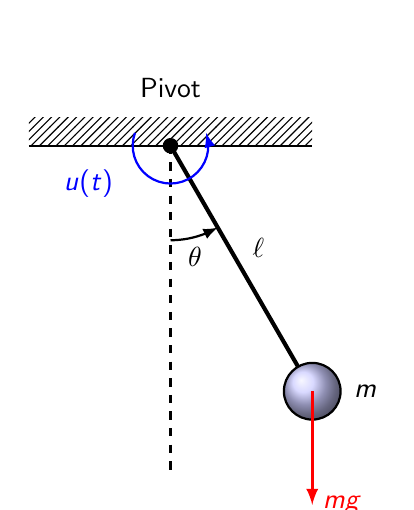
\begin{tikzpicture}[thick, >=latex, scale=1.2]
			% Ceiling
			\fill [pattern = north east lines] (-1.5,0) rectangle (1.5,0.3);
			\draw (-1.5,0) -- (1.5,0);
			
			% Pivot
			\filldraw [black] (0,0) circle (2pt);
			\node at (0,0.4) [above] {Pivot};
			
			% Dashed vertical line
			\draw [dashed] (0,0) -- (0,-3.5);
			
			% Pendulum Rod (at angle -30 degrees for illustration)
			\draw [line width=1.5pt] (0,0) -- (1.5,-2.598) node [midway, above right] {$\ell$};
			
			% Mass
			\shade [ball color=blue!20] (1.5,-2.598) circle (0.3);
			\draw (1.5,-2.598) circle (0.3) node [right=0.4cm] {$m$};
			
			% Angle theta
			\draw [->] (0,-1) arc (270:300:1) node [midway, below] {$\theta$};
			
			% Gravity vector
			\draw [->, red, line width=1pt] (1.5,-2.598) -- (1.5,-3.8) node [right] {$mg$};
			
			% Torque input
			\draw [->, blue, domain=160:380] plot ({0.4*cos(\x)}, {0.4*sin(\x)});
			\node [blue, left] at (-0.5,-0.4) {$u(t)$};
		\end{tikzpicture}
		\captionof{figure}{Pendulum system.}
		\label{fig:Pendulum}
	\end{center}
	
	\textbf{1. Physical Laws} \\
	We apply Newton's second law for rotational motion:
	\[
	\tau_{\text{net}} = I \ddot{\theta}
	\]
	where $I = m\ell^2$ is the moment of inertia and $\theta$ is the angular position measured from the vertical downward position. The torques acting on the system are:
	\begin{itemize}
		\item \textbf{Control Torque:} $+u(t)$ (applied at the pivot).
		\item \textbf{Gravity:} $-mg\ell \sin\theta$ (restoring torque).
		\item \textbf{Friction:} $-b \dot{\theta}$ (viscous damping opposing motion).
	\end{itemize}
	
	Substituting these into the equation of motion:
	\[
	m\ell^2 \ddot{\theta} = u(t) - mg\ell \sin\theta - b \dot{\theta}
	\]
	Solving for the angular acceleration $\ddot{\theta}$:
	\begin{equation*}
		\ddot{\theta} = -\frac{g}{\ell} \sin\theta - \frac{b}{m\ell^2} \dot{\theta} + \frac{1}{m\ell^2} u(t)
	\end{equation*}
	
	\textbf{2. State-Space Formulation} \\
	To convert this second-order differential equation into first-order state-space form, we define the state variables:
	\[
	x_1(t) = \theta(t) \quad \text{(Angle)}, \qquad x_2(t) = \dot{\theta}(t) \quad \text{(Angular Velocity)}
	\]
	Taking the time derivative of the state vector:
	\begin{align*}
		\dot{x}_1 &= \dot{\theta} = x_2 \\
		\dot{x}_2 &= \ddot{\theta} = -\frac{g}{\ell} \sin x_1 - \frac{b}{m\ell^2} x_2 + \frac{1}{m\ell^2} u
	\end{align*}
	
	We can now write this explicitly in the vector form $\dot{x} = f(x, u)$ introduced previously:
	\begin{equation}
		\underbrace{\begin{bmatrix} \dot{x}_1 \\[10pt] \dot{x}_2 \end{bmatrix}}_{\dot{x}(t)} 
		= 
		\underbrace{\begin{bmatrix} 
				x_2 \\[10pt]
				-\dfrac{g}{\ell} \sin(x_1) - \dfrac{b}{m\ell^2} x_2 + \dfrac{1}{m\ell^2} u 
		\end{bmatrix}}_{f(x, u)}
	\end{equation}
	
	If our objective is to measure the angle, the output equation becomes:
	\[
	y(t) = \underbrace{\begin{bmatrix} 1 & 0 \end{bmatrix} \begin{bmatrix} x_1 \\ x_2 \end{bmatrix}}_{h(x)} = x_1
	\]
	This clearly demonstrates the nonlinear nature of the system, arising from the trigonometric term $\sin(x_1)$ inside the vector function $f$.
	
	\textbf{3. Linearisation (Small Angle Approximation)} \\
	While nonlinear models capture the full physics, they are computationally expensive to use in real-time optimisation. However, for many control applications, the pendulum operates near the vertical downward equilibrium ($\theta = 0$).
	
	For small deviations from this equilibrium ($|\theta| \ll 1$ rad), we can apply the small-angle approximation:
	\[
	\sin(\theta) \approx \theta \implies \sin(x_1) \approx x_1
	\]
	Substituting this into the nonlinear state equation for $\dot{x}_2$, the dynamics become linear:
	\[
	\dot{x}_2 = -\frac{g}{\ell} x_1 - \frac{b}{m\ell^2} x_2 + \frac{1}{m\ell^2} u
	\]
	We can now rewrite the entire system in the standard LTI matrix form $\dot{x} = Ax + Bu$:
	\begin{equation}
		\underbrace{\begin{bmatrix} \dot{x}_1 \\ \dot{x}_2 \end{bmatrix}}_{\dot{x}}
		=
		\underbrace{\begin{bmatrix} 
				0 & 1 \\ 
				-\dfrac{g}{\ell} & -\dfrac{b}{m\ell^2} 
		\end{bmatrix}}_{A} 
		\underbrace{\begin{bmatrix} x_1 \\ x_2 \end{bmatrix}}_{x}
		+
		\underbrace{\begin{bmatrix} 
				0 \\ 
				\dfrac{1}{m\ell^2} 
		\end{bmatrix}}_{B} 
		u
	\end{equation}
	
	The output equation remains linear:
	\begin{equation}
		y = \underbrace{\begin{bmatrix} 1 & 0 \end{bmatrix}}_{C} x + \underbrace{\begin{bmatrix} 0 \end{bmatrix}}_{D} u
	\end{equation}
	
	This yields the familiar state-space quadruplet $(A, B, C, D)$. Throughout the majority of this course, we will focus on systems that can be described by (or approximated by) such linear models, as they allow for the use of highly efficient convex optimisation solvers (e.g., Quadratic Programming).
\end{examplebox}

\begin{notebox}{Summary}
The state vector $x(t)$ contains the minimal set of variables required to describe the system’s internal condition. Knowledge of $x(t)$ at the current time allows prediction of future states and outputs, which is precisely the information required by MPC.

For linear time-invariant (LTI) systems, which form the backbone of most MPC formulations, the model reduces to
\begin{align*}
\dot{x}(t) &= A x(t) + B u(t) \\
y(t) &= C x(t) + D u(t),
\end{align*}
with constant matrices $A$, $B$, $C$, and $D$ formed by physical parameters of the system.
\end{notebox}

\subsection*{Physical interpretation of states}

In practice, states are not abstract quantities: they usually correspond to physically meaningful variables associated with energy storage. Typical examples include:
\begin{itemize}
	\item \textbf{Electrical:} Currents in inductors and voltages across capacitors (magnetic and electric energy).
\item \textbf{Mechanical:} Positions and velocities of masses (potential and kinetic energy).
	\item \textbf{Process:} Temperatures, pressures, or concentrations (thermal and chemical potential).
\end{itemize}

This interpretation provides a systematic way to construct models from first principles. Starting from physical laws—such as Kirchhoff’s laws in electrical systems or Newton’s laws in mechanical systems—we obtain differential equations whose natural variables become the system states.

\begin{notebox}{Caveat: Intentionally incorporated states}
	It is also common to extend the state vector with non-physical variables to improve control performance. For instance, to ensure the controller eliminates steady-state error (offset-free tracking), we often add an \textbf{integrator state} or a \textbf{disturbance estimate} to the model. 
	
	These are mathematical constructs rather than physical ones, yet they are treated identically within the state-space framework. We will explore these techniques in the upcoming chapters.
\end{notebox}

\subsection*{Why does MPC rely on state-space models?}

The importance of the state-space formulation in MPC can be summarised as follows:
\begin{itemize}
	\item \textbf{Recursive Prediction:} The state-space form ($x_{k+1} = Ax_k + Bu_k$) is inherently recursive. This allows the controller to compute the future evolution of the system over a horizon $N$ simply by iterating matrix multiplications, which is computationally efficient for real-time optimisation.
	
	\item \textbf{Native MIMO Capability:} Unlike transfer functions, which require complex coupling terms to model interactions, state-space models naturally accommodate Multi-Input Multi-Output (MIMO) systems via matrix dimensions. This is essential for industrial processes where inputs are rarely isolated.
	
	\item \textbf{Direct Constraint Handling:} MPC is defined by its ability to respect limits. Physical bounds (e.g., valve positions or safety pressures) map directly onto simple linear inequalities involving the state and input vectors ($Cx + Du \leq b$), making them easy for standard solvers to process.
	
	\item \textbf{Systematic Discretisation:} While physical laws are derived in continuous time (differential equations), digital controllers operate in discrete time (difference equations). State-space theory provides exact methods (such as the Zero-Order Hold) to convert continuous models into discrete forms without losing physical insight.
\end{itemize}

\medskip
The state-space representation provides a modelling framework that connects physical intuition, mathematical analysis, and predictive control design. MPC relies on it directly.

In the following examples, we remind readers how to derive state-space models directly from physical principles in order to build intuition and highlight common modelling patterns.


\begin{examplebox}{State--Space Modelling of an RLC Circuit}
	
	Consider the electrical circuit shown in Figure~\ref{fig:RLC01}, consisting of a voltage source $V_i$, resistors $R_1$ and $R_2$, an inductor $L$, and a capacitor $C$. Write state equations in matrix form.
		\begin{center}
		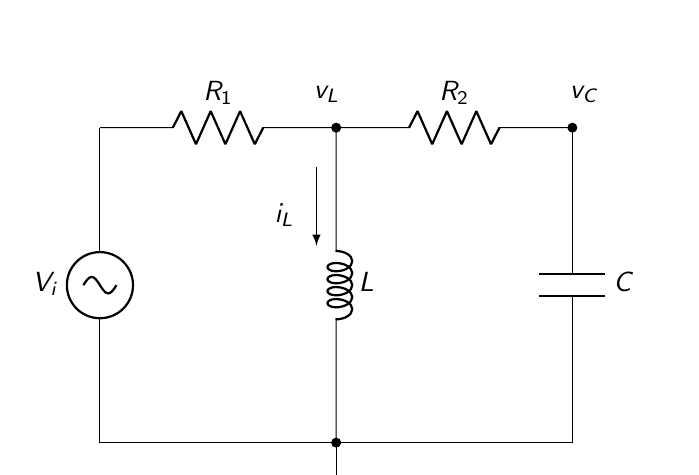
\begin{tikzpicture}
			% Paths, nodes and wires:
			\draw (2, 5) to[sinusoidal voltage source, l={$V_i$}] (2, 9);
			\draw (2, 9) to[american resistor, l={$R_1$}] (5, 9);
			\node[circ] at (5, 9){};
			\draw (5, 9) to[cute inductor, l={$L$}] (5, 5);
			\draw (5, 9) to[american resistor, l={$R_2$}] (8, 9);
			\node[circ] at (8, 9){};
			\draw (8, 9) to[capacitor, l={$C$}] (8, 5);
			\node[circ] at (5, 5){};
			\draw (8, 5) -- (5, 5) -- (2, 5);
			\node[ground] at (5, 5){};
			\draw[-latex] (4.75, 8.5) -- (4.75, 7.5);
			\node[shape=rectangle, minimum width=1.465cm,
			minimum height=0.715cm] at (4.75, 7.875){}
			node[anchor=north west, align=left,
			text width=1.077cm, inner sep=6pt] at (4, 8.25){$i_L$};
			\node[shape=rectangle, minimum width=1.465cm,
			minimum height=0.465cm] at (5.25, 9.5){}
			node[anchor=north west, align=left,
			text width=1.077cm, inner sep=6pt] at (4.5, 9.75){$v_L$};
			\node[shape=rectangle, minimum width=1.465cm,
			minimum height=0.465cm] at (8.5, 9.5){}
			node[anchor=north west, align=left,
			text width=1.077cm, inner sep=6pt] at (7.75, 9.75){$v_C$};
		\end{tikzpicture}
		\captionof{figure}{An RLC circuit.}
		\label{fig:RLC01}
	\end{center}
	
	\medskip
	\solution
	We select the energy variables as state variables:
	\[
	x_1 = i_L \quad \text{(inductor current)}, 
	\qquad 
	x_2 = v_C \quad \text{(capacitor voltage)},
	\]
	and take the input as
	\[
	u = v_i .
	\]
	
We begin with the constitutive relations of the energy–storage elements. 
Since the state variables are chosen as the inductor current and the capacitor voltage, all other variables are expressed in terms of these states and the input.
\begin{align}
	v_L &= L \frac{d i_L}{dt}, \\
	i_C &= C \frac{d v_C}{dt}.
\end{align}

The current flowing through resistor $R_2$ is given by Ohm’s law as
\[
i_{R_2} = \frac{v_L - v_C}{R_2}.
\]
Applying Kirchhoff’s Current Law (KCL) at node $v_C$ and noting that the capacitor current equals the current through $R_2$ yields
\[
C \dot{v}_C = \frac{v_L - v_C}{R_2}.
\]
	
	Applying KCL at node $v_L$ yields
	\[
	\frac{v_i - v_L}{R_1} = i_L + \frac{v_L - v_C}{R_2}.
	\]
	
	Solving for $v_L$:
	\[
	v_L =
	\frac{R_2}{R_1 + R_2} v_i
	- \frac{R_1 R_2}{R_1 + R_2} i_L
	+ \frac{R_1}{R_1 + R_2} v_C .
	\]
	
	\medskip
	\textbf{State equations.}
	Substituting $v_L$ into the inductor and capacitor equations gives
	\begin{align}
		 \frac{d}{dt}{i}_L &=
		-\frac{R_1 R_2}{L(R_1 + R_2)} i_L
		+ \frac{R_1}{L(R_1 + R_2)} v_C
		+ \frac{R_2}{L(R_1 + R_2)} v_i, \\[6pt]
		 \frac{d}{dt}{v}_C &=
		-\frac{R_1}{C(R_1 + R_2)} i_L
		-\frac{1}{C(R_1 + R_2)} v_C
		+ \frac{1}{C(R_1 + R_2)} v_i.
	\end{align}
	
	\medskip
	\textbf{State--space representation.}
	Defining the state vector $x = [\, i_L \;\; v_C \,]^\top$, the system can be written compactly as
	\[
	\dot{x} = A x + B u,
	\]
	where
	\[
	A =
	\begin{bmatrix}
		-\dfrac{R_1 R_2}{L(R_1 + R_2)} & \dfrac{R_1}{L(R_1 + R_2)} \\[8pt]
		-\dfrac{R_1}{C(R_1 + R_2)} & -\dfrac{1}{C(R_1 + R_2)}
	\end{bmatrix},
	\qquad
	B =
	\begin{bmatrix}
		\dfrac{R_2}{L(R_1 + R_2)} \\[8pt]
		\dfrac{1}{C(R_1 + R_2)}
	\end{bmatrix}.
	\]

\end{examplebox}



\begin{examplebox}{Mass--Spring--Damper with External Forcing (State--Space Modelling)}
	\textbf{Question.}
	A mass--spring--damper system shown in Figure~\ref{fig:MDS_system} is subjected to an external force input $F(t)$. The displacement of the mass from equilibrium is denoted by $\zeta(t)$ (positive to the right). The system parameters are mass $m$, damping coefficient $c$, and spring stiffness $k$.
	
	\medskip
	\begin{center}
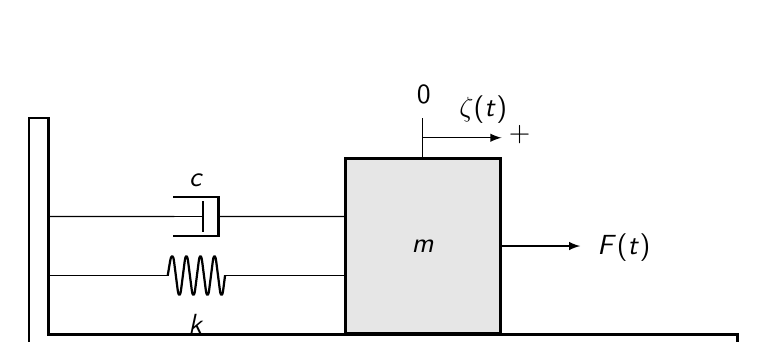
\begin{tikzpicture}
	% Paths, nodes and wires:
	\path[draw={rgb,255:red,0;green,0;blue,0}, line width=1pt] (1, 8.5) -| (1, 6.5) -| (10, 6.75) |- (1.25, 6.75) -- (1.25, 9.5) -| (1, 8.5);
	\draw (1.25, 7.5) to[spring, l_={$k$}] (5, 7.5);
	\draw (1.25, 8.25) to[damper, l={$c$}] (5, 8.25);
	\node[shape=rectangle, fill={rgb,255:red,145;green,145;blue,145}, fill opacity=0.23, draw, line width=1pt, minimum width=1.965cm, minimum height=2.215cm](N1) at (6, 7.875){} node[anchor=center] at (N1.text){$m$};
	\draw[-latex] (7, 7.875) -- (8, 7.875);
	\draw[-latex] (6, 9.25) -- (7, 9.25);
	\node[shape=rectangle, minimum width=1.215cm, minimum height=0.715cm] at (8.625, 7.875){} node[anchor=north west, align=left, text width=0.827cm, inner sep=6pt] at (8, 8.25){$F(t)$};
	\node[shape=rectangle, minimum width=1.215cm, minimum height=0.715cm] at (6.872, 9.625){} node[anchor=north west, align=left, text width=0.827cm, inner sep=6pt] at (6.247, 10){$\zeta(t)$};
	\node[shape=rectangle, minimum width=1.215cm, minimum height=0.715cm] at (7.5, 9.25){} node[anchor=north west, align=left, text width=0.827cm, inner sep=6pt] at (6.875, 9.625){$+$};
	\draw (6, 9) -| (6, 9.5);
	\node[shape=rectangle, minimum width=1.215cm, minimum height=0.715cm] at (6.331, 9.753){} node[anchor=north west, align=left, text width=0.827cm, inner sep=6pt] at (5.706, 10.128){$0$};
\end{tikzpicture}
	\captionof{figure}{Mass-damper-spring system.}
\label{fig:MDS_system}
	\end{center}
	
	\medskip
	\begin{enumerate}
		\item Write the equation of motion for the system in terms of $\zeta(t)$, $\dot{\zeta}(t)$, $\ddot{\zeta}(t)$, and the input force $F(t)$.
		\item Choose a suitable state vector and write the continuous-time state-space model
		\[
		\dot{x}(t) = A x(t) + B u(t),
		\]
		clearly defining $x(t)$ and $u(t)$.
		\item If the output is the displacement, i.e.\ $y(t)=\zeta(t)$, write the output equation
		\[
		y(t) = C x(t) + D u(t).
		\]
	\end{enumerate}
	\medskip
	\solution
	\textbf{1) Equation of motion:}
	Let $\zeta(t)$ denote the displacement of the mass from equilibrium (positive to the right), and let $F(t)$ be the applied external force. By Newton’s second law, the sum of forces on the mass equals $m\ddot{\zeta}(t)$. The spring force is $-k\zeta(t)$ and the damper force is $-c\dot{\zeta}(t)$. Hence,
	\[
	m\ddot{\zeta}(t) = F(t) - c\dot{\zeta}(t) - k\zeta(t),
	\]
	or equivalently,
	\[
	m\ddot{\zeta}(t) + c\dot{\zeta}(t) + k\zeta(t) = F(t).
	\]
	
	\medskip
	\textbf{2) Choice of states and state equations:}
	Choose the standard second-order state variables
	\[
	x_1(t)=\zeta(t), 
	\qquad 
	x_2(t)=\dot{\zeta}(t),
	\qquad 
	u(t)=F(t).
	\]
	Then
	\[
	\dot{x}_1(t) = x_2(t),
	\]
	and, from the equation of motion,
	\[
	\dot{x}_2(t)=\ddot{\zeta}(t) = -\frac{k}{m}x_1(t) - \frac{c}{m}x_2(t) + \frac{1}{m}u(t).
	\]
	
	\medskip
	\textbf{3) State-space form:}
	Defining $x(t)=\begin{bmatrix}x_1(t)\\x_2(t)\end{bmatrix}$, the system can be written as
	\[
	\dot{x}(t)=A x(t)+B u(t),
	\]
	with
	\[
	A=
	\begin{bmatrix}
		0 & 1\\[4pt]
		-\dfrac{k}{m} & -\dfrac{c}{m}
	\end{bmatrix},
	\qquad
	B=
	\begin{bmatrix}
		0\\[4pt]
		\dfrac{1}{m}
	\end{bmatrix}.
	\]
	
	\medskip
	\textbf{4) Output equation.}
	If the measured output is the displacement $y(t)=\zeta(t)=x_1(t)$, then
	\[
	y(t)=C x(t)+D u(t),
	\]
	where
	\[
	C=\begin{bmatrix}1 & 0\end{bmatrix},
	\qquad
	D=\begin{bmatrix}0\end{bmatrix}.
	\]
	
\end{examplebox}

\section{Nonlinear Systems and Local Linearisation}

Many real-world systems are inherently nonlinear. Nonlinearities may arise from physical laws, geometric effects, saturation, friction, or actuator limits. While linear state-space models play a central role in MPC, they are often obtained as local approximations of an underlying nonlinear system.

In this section, we introduce nonlinear state-space models, define equilibrium points, and show how nonlinear dynamics can be approximated locally using Taylor expansion. This leads naturally to the concept of Jacobian linearisation.

\subsection{Nonlinear state-space models}

A general nonlinear continuous-time system is described by
\begin{align*}
\dot{x}(t) &= f\big(x(t), u(t)\big) \\
y(t) &= h\big(x(t), u(t)\big),
\end{align*}
where the functions $f(\cdot)$ and $h(\cdot)$ are nonlinear mappings.

Unlike linear systems, nonlinear systems:
\begin{itemize}
	\item may have multiple equilibrium points,
	\item exhibit behaviour that depends strongly on the operating point,
	\item cannot, in general, be analysed using superposition.
\end{itemize}

For MPC design, it is common to operate the system near a desired steady state. Linearisation provides a systematic way to approximate the nonlinear dynamics locally around such an operating point.

\subsection{Equilibrium points}

An equilibrium point represents a state of operation where the system's dynamic evolution ceases. If a system is initialised at an equilibrium state and the external inputs remain constant, the state will not change over time.

We distinguish between the definitions for continuous-time and discrete-time systems below.

\begin{defnbox}{Definition: Equilibrium Points}
	\textbf{1. Continuous-Time Case:} \\
	For a continuous-time system $\dot{x}(t) = f(x(t), u(t))$, an equilibrium point is a pair $(x_e, u_e)$ such that the time derivative vanishes:
	\begin{equation}
		f(x_e, u_e) = 0
	\end{equation}
	
	\textbf{2. Discrete-Time Case:} \\
	For a discrete-time system $x_{k+1} = f(x_k, u_k)$, an equilibrium point is a pair $(x_e, u_e)$ such that the next state is identical to the current state (a fixed point):
	\begin{equation}
		x_e = f(x_e, u_e)
	\end{equation}
\end{defnbox}

\subsection*{Determination of Equilibria}
To find the equilibrium points for a given constant input $u_e$, one must solve a set of algebraic equations:
\begin{itemize}
	\item \textbf{Continuous:} Solve the system of equations $f(x, u_e) = 0$ for $x$.
	\item \textbf{Discrete:} Solve the fixed-point equation $x - f(x, u_e) = 0$ for $x$.
\end{itemize}
Note that nonlinear systems may have multiple equilibrium points, a single unique equilibrium, or no equilibrium points at all for a specific input.

\subsection*{Physical Interpretation}
In engineering contexts, equilibrium points are often referred to as \textit{operating points}, \textit{trim points}, or \textit{steady states}. Physically, they correspond to:
\begin{itemize}
	\item \textbf{Mechanical Systems:} A position of rest (velocity and acceleration are zero) or motion at a constant velocity (acceleration is zero).
	\item \textbf{Thermal/Chemical Systems:} A state where inflows equal outflows, resulting in constant temperature, pressure, or concentration.
	\item \textbf{Electrical Systems:} A state where capacitor voltages and inductor currents have settled to constant DC values.
\end{itemize}
Ideally, a control system is designed to steer the dynamic system from an arbitrary initial state towards a desired equilibrium point $(x_{ref}, u_{ref})$.


\subsection{Local approximation via Taylor expansion}

To analyse system behaviour near an equilibrium, we approximate the nonlinear dynamics using a Taylor series expansion.

\subsubsection*{Scalar case}

Consider a scalar nonlinear system
\[
\dot{x} = f(x,u),
\]
and let $(x_e,u_e)$ be an equilibrium point.

The first-order Taylor expansion of $f(x,u)$ about $(x_e,u_e)$ is
\[
f(x,u) \approx f(x_e,u_e)
+ \frac{\partial f}{\partial x}\Big|_{(x_e,u_e)} (x-x_e)
+ \frac{\partial f}{\partial u}\Big|_{(x_e,u_e)} (u-u_e).
\]

Since $f(x_e,u_e)=0$ at equilibrium, this simplifies to
\[
\dot{x} \approx 
\frac{\partial f}{\partial x}\Big|_{(x_e,u_e)} (x-x_e)
+ \frac{\partial f}{\partial u}\Big|_{(x_e,u_e)} (u-u_e).
\]

This expression describes a \emph{linear approximation} of the nonlinear system near the equilibrium.

\subsubsection*{Multivariable case}

Now consider the nonlinear vector-valued system
\[
\dot{x} = f(x,u), 
\qquad 
x \in \mathbb{R}^n, \; u \in \mathbb{R}^m.
\]

Expanding $f(x,u)$ about the equilibrium $(x_e,u_e)$ yields
\[
f(x,u) \approx f(x_e,u_e)
+ \frac{\partial f}{\partial x}\Big|_{(x_e,u_e)} (x-x_e)
+ \frac{\partial f}{\partial u}\Big|_{(x_e,u_e)} (u-u_e).
\]

Again using $f(x_e,u_e)=0$, we obtain
\[
\dot{x} \approx A (x-x_e) + B (u-u_e),
\]
where the matrix
\[
A = \left.\frac{\partial f}{\partial x}\right|_{(x_e,u_e)} 
 =
\left[
\begin{array}{cccc}
	\dfrac{\partial f_1}{\partial x_1} &
	\dfrac{\partial f_1}{\partial x_2} &
	\cdots &
	\dfrac{\partial f_1}{\partial x_n} \\[8pt]
	
	\dfrac{\partial f_2}{\partial x_1} &
	\dfrac{\partial f_2}{\partial x_2} &
	\cdots &
	\dfrac{\partial f_2}{\partial x_n} \\[4pt]
	
	\vdots & \vdots & \ddots & \vdots \\[4pt]
	
	\dfrac{\partial f_n}{\partial x_1} &
	\dfrac{\partial f_n}{\partial x_2} &
	\cdots &
	\dfrac{\partial f_n}{\partial x_n}
\end{array}
\right]_{(x_e,u_e)}.
\]

Note that each entry $A_{ij}$ represents the sensitivity of the $i$th state equation to the $j$th state variable, evaluated at the equilibrium point.

Similarly, 
\[
B = \left.\frac{\partial f}{\partial u}\right|_{(x_e,u_e)} =
\left[
\begin{array}{cccc}
	\dfrac{\partial f_1}{\partial u_1} &
	\dfrac{\partial f_1}{\partial u_2} &
	\cdots &
	\dfrac{\partial f_1}{\partial u_m} \\[8pt]
	
	\dfrac{\partial f_2}{\partial u_1} &
	\dfrac{\partial f_2}{\partial u_2} &
	\cdots &
	\dfrac{\partial f_2}{\partial u_m} \\[4pt]
	
	\vdots & \vdots & \ddots & \vdots \\[4pt]
	
	\dfrac{\partial f_n}{\partial u_1} &
	\dfrac{\partial f_n}{\partial u_2} &
	\cdots &
	\dfrac{\partial f_n}{\partial u_m}
\end{array}
\right]_{(x_e,u_e)}.
\]

Each entry $B_{ij}$ quantifies how the $j$th input influences the $i$th state equation in the neighbourhood of the equilibrium.

\medskip
\noindent
With these matrices, the linearised dynamics in deviation variables
\[
\tilde{x} = x - x_e,
\qquad
\tilde{u} = u - u_e
\]
are given by
\[
\dot{\tilde{x}} = A \tilde{x} + B \tilde{u}.
\]

If the output equation is nonlinear,
\[
y = h(x,u),
\]
a similar expansion gives
\[
\tilde{y} = C \tilde{x} + D \tilde{u},
\]
with
\[
C = \left.\frac{\partial h}{\partial x}\right|_{(x_e,u_e)},
\qquad
D = \left.\frac{\partial h}{\partial u}\right|_{(x_e,u_e)}.
\]

\medskip


\begin{examplebox}{Nonlinear Planar Duorotor}
	\textbf{Question:}
	The nonlinear dynamics of a planar duorotor (shown in Figure~\ref{fig:duorotor_model}) with mass $m$, inertia $J$, and arm length $\ell$ are given by:
	\begin{align*}
		m\ddot{p}_x &= -(u_1+u_2)\sin(\theta) \\
		m\ddot{p}_y &= (u_1+u_2)\cos(\theta) - mg \\
		J\ddot{\theta} &= \frac{\ell }{2}(u_2 - u_1)
	\end{align*}
	where $p_x$ is the horizontal position and $p_y$ is the vertical position.
	Linearise these dynamics around the hover equilibrium ($\theta=0, u_1=u_2=mg/2$) to obtain an LTI state-space model, $\dot{{x}} = A{x} + B{u}$.
	
\begin{center}
		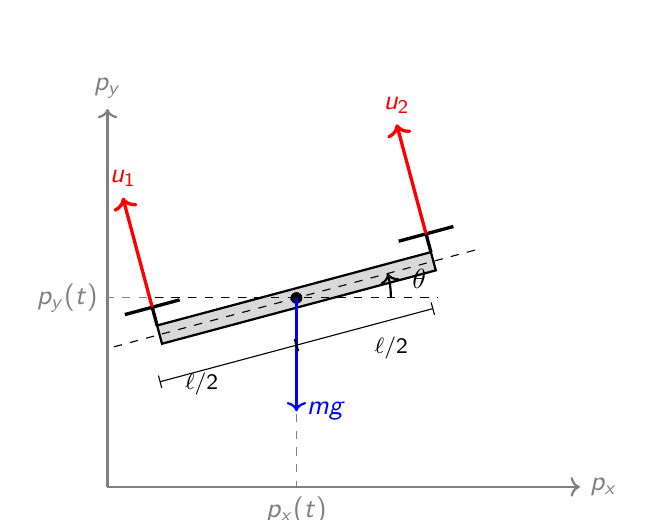
\begin{tikzpicture}[scale=1.2]
			% Define parameters
			\def\angle{15} % Tilt angle for visualization
			\def\px{2}     % Position x
			\def\py{2}     % Position y
			\def\arm{1.5}  % Half arm length
			
			% Inertial Frame / Axes
			\draw[->, thick, gray] (0,0) -- (5,0) node[right] {$p_x$};
			\draw[->, thick, gray] (0,0) -- (0,4) node[above] {$p_y$};
			
			% Dashed lines for position projection
			\draw[dashed, gray] (\px, \py) -- (\px, 0) node[below] {$p_x(t)$};
			\draw[dashed, gray] (\px, \py) -- (0, \py) node[left] {$p_y(t)$};
			
			% Drone Local Frame (Rotated)
			\begin{scope}[shift={(\px,\py)}, rotate=\angle]
				% Body
				\draw[thick, fill=gray!30] (-\arm, -0.1) rectangle (\arm, 0.1);
				\node[circle, fill=black, inner sep=1.5pt] at (0,0) {}; % CoM
				
				% Left Rotor (u1)
				\draw[very thick] (-\arm, 0.1) -- (-\arm, 0.3);
				\draw[very thick] (-\arm-0.3, 0.3) -- (-\arm+0.3, 0.3);
				\draw[->, very thick, red] (-\arm, 0.3) -- (-\arm, 1.5) node[above] {$u_1$};
				
				% Right Rotor (u2)
				\draw[very thick] (\arm, 0.1) -- (\arm, 0.3);
				\draw[very thick] (\arm-0.3, 0.3) -- (\arm+0.3, 0.3);
				\draw[->, very thick, red] (\arm, 0.3) -- (\arm, 1.5) node[above] {$u_2$};
				
				% Body axis line for angle measurement
				\draw[dashed] (-\arm-0.5, 0) -- (\arm+0.5, 0);
			\end{scope}
			
			% Horizontal reference at CoM for angle theta
			\draw[dashed] (\px-1.5, \py) -- (\px+1.5, \py);
			
			% Angle arc
			\draw[->, thick] (\px+1.0, \py) arc (0:\angle:1.0);
			\node at (\px+1.3, \py+0.2) {$\theta$};
			
			% Gravity Vector
			\draw[->, thick, blue] (\px, \py) -- (\px, \py-1.2) node[right] {$mg$};
			
			% Dimensions (Arm length)
			\draw[|-|] (\px, \py-0.5) -- ++(\angle:\arm) node[midway, below right, font=\footnotesize] {$\ell/2$};
			\draw[|-|] (\px, \py-0.5) -- ++(\angle+180:\arm) node[midway, below left, font=\footnotesize] {$\ell/2$};
			
		\end{tikzpicture}
		\captionof{figure}{Planar duorotor model showing states ($p_x, p_y, \theta$) and inputs ($u_1, u_2$). The coordinate system is inertial, with $\theta$ measured counter-clockwise from the vertical (upward).}
		\label{fig:duorotor_model}
\end{center}
	
	
	\medskip
	\solution
	\textbf{1) Define states and inputs:}
	We select the state vector such that the generalized coordinates appear first, followed by their velocities:
	\[
	x(t) = 
	\begin{bmatrix} x_1 & x_2 & x_3 & x_4 & x_5 & x_6 \end{bmatrix}^\top
	=
	\begin{bmatrix} p_x & p_y & \theta & \dot{p}_x & \dot{p}_y & \dot{\theta} \end{bmatrix}^\top.
	\]
	The input vector is $u = [\, u_1 \;\; u_2 \,]^\top$.
	
	The nonlinear state-space equations $\dot{x} = f(x,u)$ are:
	\begin{align*}
		\dot{x}_1 &= x_4, \\
		\dot{x}_2 &= x_5, \\
		\dot{x}_3 &= x_6, \\
		\dot{x}_4 &= -\frac{1}{m}(u_1+u_2)\sin(x_3), \\
		\dot{x}_5 &= \frac{1}{m}(u_1+u_2)\cos(x_3) - g, \\
		\dot{x}_6 &= \frac{\ell}{2J}(u_2 - u_1).
	\end{align*}
	
	\textbf{2) Determine the equilibrium point:}
	At hover, the drone is stationary at the origin with zero angle:
	\[
	x_e = [\, 0 \;\; 0 \;\; 0 \;\; 0 \;\; 0 \;\; 0 \,]^\top.
	\]
	Setting accelerations ($\dot{x}_4, \dot{x}_5, \dot{x}_6$) to zero:
	\begin{itemize}
		\item From $\dot{x}_5=0$: $\dfrac{1}{m}(u_{1,e}+u_{2,e})\cos(0) - g = 0 \implies u_{1,e}+u_{2,e} = mg$.
		\item From $\dot{x}_6=0$: $\dfrac{\ell}{2J}(u_{2,e}-u_{1,e}) = 0 \implies u_{1,e} = u_{2,e}$.
	\end{itemize}
	Thus, the equilibrium inputs are $u_{1,e} = u_{2,e} = \dfrac{mg}{2}$.
	
	\medskip
	\textbf{3) Jacobian Linearisation:}
	We compute the Jacobian matrices $A = \dfrac{\partial f}{\partial x}$ and $B = \frac{\partial f}{\partial u}$ evaluated at $(x_e, u_e)$.
	
	For matrix $A$:
	Rows 1--3 are purely kinematic ($\dot{p} = v$), resulting in an identity matrix in the top-right block. For rows 4--6, we check the derivatives with respect to the angle $\theta$ (state $x_3$):
	\begin{align*}
		\frac{\partial \dot{x}_4}{\partial x_3} \bigg|_{eq} &= -\frac{u_{1,e}+u_{2,e}}{m}\cos(x_{3,e}) = -\frac{mg}{m}(1) = -g, \\
		\frac{\partial \dot{x}_5}{\partial x_3} \bigg|_{eq} &= -\frac{u_{1,e}+u_{2,e}}{m}\sin(x_{3,e}) = -\frac{mg}{m}(0) = 0.
	\end{align*}
	
	For matrix $B$:
	We compute derivatives of the accelerations with respect to inputs $u_1$ and $u_2$:
	\begin{align*}
		\frac{\partial \dot{x}_4}{\partial u} \bigg|_{eq} &= -\frac{1}{m}\sin(x_{3,e}) = 0, \\
		\frac{\partial \dot{x}_5}{\partial u} \bigg|_{eq} &= \frac{1}{m}\cos(x_{3,e}) = \frac{1}{m}.
	\end{align*}
	The angular acceleration $\dot{x}_6$ remains linear in $u$, with coefficients $\mp \frac{\ell}{2J}$.
	
	\medskip
	\textbf{4) Final State-Space Model:}
	Substituting these values, we obtain the linearised model $\dot{\tilde{x}} = A \tilde{x} + B \tilde{u}$:
	\[
	A = 
	\begin{bmatrix}
		0 & 0 & 0 & 1 & 0 & 0 \\
		0 & 0 & 0 & 0 & 1 & 0 \\
		0 & 0 & 0 & 0 & 0 & 1 \\
		0 & 0 & -g & 0 & 0 & 0 \\
		0 & 0 & 0 & 0 & 0 & 0 \\
		0 & 0 & 0 & 0 & 0 & 0
	\end{bmatrix},
	\quad
	B = 
	\begin{bmatrix}
		0 & 0 \\
		0 & 0 \\
		0 & 0 \\
		0 & 0 \\
		\dfrac{1}{m} & \dfrac{1}{m} \\[4pt]
		-\dfrac{\ell}{2J} & \dfrac{\ell}{2J}
	\end{bmatrix}.
	\]
	where $\tilde{x} = x - x_e$ and $\tilde{u} = u - u_e$.
\end{examplebox}



\section{Obtaining DT Realisation of CT LTI State-space systems}

For a homogeneous LTI system $\dot{{x}} = {A}{x}$, the state at a future time $t+\Delta t$ is given by:
\begin{equation}
	{x}(t+\Delta t) = e^{{A}\Delta t} {x}(t)
\end{equation}
The term $e^{{A}\Delta t}$ is the matrix exponential. It is not computed element-wise; rather, it is defined by the infinite Taylor series expansion:
\[
e^{{M}} = {I} + {M} + \frac{1}{2!}{M}^2 + \frac{1}{3!}{M}^3 + \cdots
\]
In MATLAB, this is computed efficiently using the \texttt{expm()} function.

\subsection{Exact Discretisation of LTI Systems}
This analytical solution gives us a way to \textit{exactly} discretise a linear system. If we choose a fixed time step $h = \Delta t$, the discrete-time dynamics are:
\begin{equation}
	{x}_{k+1} = {A}_d {x}_k \quad \text{where} \quad {A}_d = e^{{A}h}
\end{equation}
This is fundamentally different from numerical integrators like Euler or RK4, which are approximations. For LTI systems, the matrix exponential provides the exact transition matrix ${A}_d$.

\begin{table}[h!]
	\centering
	\begin{tabular}{|l|l|}
		\hline
		\textbf{Linear Systems} & \textbf{Nonlinear Systems} \\
		\hline
		$\dot{{x}} = {A}{x}$ & $\dot{{x}} = {f}({x})$ \\
		Can be solved exactly in closed form. & Almost never have closed-form solutions. \\
		Discretised exactly using $e^{{A}h}$. & Discretised approximately using numerical \\
		& integrators (Euler, RK4, ODE45, etc.). \\
		\hline
	\end{tabular}
	\caption{Comparison of solving linear vs. nonlinear ODEs.}
\end{table}


\section{Discretisation of Forced Linear Systems}

How do we discretise a forced system $\dot{{x}} = {A}{x} + {B}{u}$? The matrix exponential only applies to homogeneous systems (of the form $\dot{{z}} = {T}{z}$). We can use a clever trick: augment the state to absorb the input and then apply the matrix exponential.

First, we must assume something about how the control input ${u}(t)$ behaves \textit{between} discrete time steps. The most common assumption is a \emph{Zero-Order Hold (ZOH)}, which means the control input is held constant over each time step:
\[
{u}(t) = {u}_k \quad \text{for} \quad t \in [t_k, t_{k+1})
\]
This is equivalent to stating that the derivative of the input is zero during the interval: $\dot{{u}} = {0}$.

With the ZOH assumption, we can create an augmented state vector ${z} = [{x}^T, {u}^T]^T$. The dynamics of this new state are:
\[
\dot{{z}} = \begin{bmatrix} \dot{{x}} \\ \dot{{u}} \end{bmatrix} = \begin{bmatrix} {A}{x} + {B}{u} \\ {0} \end{bmatrix} = \underbrace{\begin{bmatrix} {A} & {B} \\ {0} & {0} \end{bmatrix}}_{{T}} \begin{bmatrix} {x} \\ {u} \end{bmatrix} = {T}{z}
\]
We now have a larger, but homogeneous, linear system. We can apply the matrix exponential to find its exact discrete-time solution:
\[
{z}_{k+1} = e^{{T}h} {z}_k \implies \begin{bmatrix} {x}_{k+1} \\ {u}_{k+1} \end{bmatrix} = e^{\begin{bmatrix} {A} & {B} \\ {0} & {0} \end{bmatrix}h} \begin{bmatrix} {x}_k \\ {u}_k \end{bmatrix}
\]
The matrix exponential of this block matrix has a special structure that gives us our final discrete-time system:
\[
e^{{T}h} = \begin{bmatrix} {A}_d & {B}_d \\ {0} & {I} \end{bmatrix}
\]
Expanding the equation for ${x}_{k+1}$ gives the standard discrete-time form:
\begin{equation}\label{eqn:stateEquation}
	{x}_{k+1} = {A}_d {x}_k + {B}_d {u}_k
\end{equation}


\begin{lstlisting}[language=Matlab, caption={MATLAB code to perform ZOH discretization of a forced LTI system.}, label={lst:matlab_zoh}]
	% Define a continuous-time LTI system
	A = [0, 1; -5, -2]; % Example A matrix
	B = [0; 1];         % Example B matrix
	h = 0.1;            % Time step
	
	n = size(A, 1); % Number of states
	m = size(B, 2); % Number of inputs
	
	% Form the augmented matrix T
	T = [A, B; 
		  zeros(m, n), zeros(m, m)];
	
	% Compute the matrix exponential of T*h
	M = expm(T * h);
	
	% Extract the discrete-time matrices Ad and Bd
	Ad = M(1:n, 1:n);
	Bd = M(1:n, n+1:end);
	
	disp('Ad = '); disp(Ad);
	disp('Bd = '); disp(Bd);
\end{lstlisting}

\section{Numerical Discretisation of Nonlinear Systems}

In the previous sections, we established that Linear Time-Invariant (LTI) systems can be discretised \emph{exactly} using the matrix exponential ($e^{Ah}$). However, the majority of physical systems—such as robotic arms, chemical reactors, and aerial vehicles—are inherently nonlinear:
\[
\dot{x}(t) = f(x(t), u(t)).
\]
For these systems, a closed-form solution for $x(t)$ rarely exists. To implement MPC, or to simulate these systems on a computer, we must approximate the continuous-time evolution using numerical integration methods.

In digital control, we typically assume a Zero-Order Hold (ZOH) on the input, meaning the control input is held constant over the sampling interval $h$:
\[
u(t) = u_k \quad \text{for} \quad t \in [t_k, t_{k+1}).
\]

\subsection{Forward Euler Method}
The simplest numerical approach is the Forward Euler method, which approximates the derivative as a constant slope evaluated at the beginning of the interval. It is derived from the first-order truncation of the Taylor series:
\begin{equation}
	x_{k+1} = x_k + h \cdot f(x_k, u_k).
\end{equation}

While Euler's method is algebraically simple and easy to differentiate (which is useful for optimization gradients), it suffers from significant drawbacks.

\begin{alertbox}{Warning: Avoid Euler's Method}
	Forward Euler is a first-order method, meaning the global error scales linearly with the step size ($\mathcal{O}(h)$). It is notoriously inaccurate and numerically unstable for \emph{stiff} systems (systems with fast dynamics). 
	
	Using Euler's method can introduce artificial energy into the simulation, causing stable physical systems to appear unstable (blow up) unless the time step $h$ is chosen to be infinitesimally small. {For this reason, Forward Euler should generally be avoided for accurate simulation of physical plants.}
\end{alertbox}

\subsection{Runge--Kutta 4 (RK4) Method}
The standard workhorse for engineering simulation is the 4th-order Runge--Kutta (RK4) method. Rather than relying on a single slope calculation, RK4 takes a weighted average of four slopes calculated at different points within the time step.

Given the current state $x_k$, input $u_k$, and time step $h$, the update is calculated as follows:
\begin{align*}
	k_1 &= f(x_k, u_k) \nonumber \\
	k_2 &= f\left(x_k + \frac{h}{2} k_1, u_k\right) \nonumber \\
	k_3 &= f\left(x_k + \frac{h}{2} k_2, u_k\right) \nonumber \\
	k_4 &= f(x_k + h k_3, u_k) \nonumber \\
	x_{k+1} &= x_k + \frac{h}{6} (k_1 + 2k_2 + 2k_3 + k_4).
\end{align*}
The RK4 method has a global error of $\mathcal{O}(h^4)$, providing a significantly higher degree of accuracy and stability than Euler's method for the same time step.

\begin{examplebox}{MATLAB Implementation: RK4 Integrator}
	A robust implementation of a single RK4 step in MATLAB for a generic nonlinear system:
	
	\begin{lstlisting}[language=Matlab]
		function x_next = rk4_step(f_dynamics, x_curr, u_curr, h)
			% f_dynamics: Function handle @(x,u) ...
			% x_curr:     Current state vector [n x 1]
			% u_curr:     Current input vector [m x 1]
			% h:          Time step (dt)
		
			k1 = f_dynamics(x_curr, u_curr);
			k2 = f_dynamics(x_curr + 0.5*h*k1, u_curr);
			k3 = f_dynamics(x_curr + 0.5*h*k2, u_curr);
			k4 = f_dynamics(x_curr + h*k3, u_curr);
		
			x_next = x_curr + (h/6)*(k1 + 2*k2 + 2*k3 + k4);
		end
	\end{lstlisting}
\end{examplebox}

\begin{examplebox}{Comparison of Numerical Integrators: The Harmonic Oscillator}
	\textbf{System Description} \\
	Consider a simple undamped mass-spring system (harmonic oscillator) with mass $m=1$ and spring constant $k=1$. The equation of motion is:
	\[
	\ddot{p}(t) + p(t) = 0
	\]
	We define the state vector $x = [x_1, x_2]^\top = [p, \dot{p}]^\top$. The continuous-time dynamics $\dot{x} = f(x)$ are:
	\[
	\frac{d}{dt} \begin{bmatrix} x_1 \\ x_2 \end{bmatrix} 
	= 
	\begin{bmatrix} x_2 \\ -x_1 \end{bmatrix}.
	\]
	The exact analytical solution for an initial condition $x_0 = [1, 0]^\top$ is a perfect sinusoid, $x_1(t) = \cos(t)$, which represents a circle in the phase plane (energy is conserved).
	
	\medskip
	\textbf{1. Forward Euler Discretisation} \\
	Applying the Euler update law $x_{k+1} = x_k + h f(x_k)$ yields:
	\begin{align*}
		x_{1, k+1} &= x_{1,k} + h \cdot x_{2,k} \\
		x_{2, k+1} &= x_{2,k} - h \cdot x_{1,k}
	\end{align*}
	Notice that the new state depends linearly on the current slope.
	
	\medskip
	\textbf{2. Runge--Kutta 4 (RK4) Discretisation} \\
	Applying the RK4 method requires four evaluations of the dynamics function $f(x)$ per step:
	\begin{align*}
		k_1 &= f(x_k) \\
		k_2 &= f(x_k + 0.5 h k_1) \\
		k_3 &= f(x_k + 0.5 h k_2) \\
		k_4 &= f(x_k + h k_3)
	\end{align*}
	\[
	x_{k+1} = x_k + \frac{h}{6}(k_1 + 2k_2 + 2k_3 + k_4).
	\]
	
	\medskip
	\textbf{Simulation Results} \\
	Figure~\ref{fig:integrator_comparison} compares these two methods against the exact solution across different sampling times $h$. 
	
	It can be observed that the \textbf{Forward Euler} method is numerically unstable for every selection of sampling time $h$; it introduces artificial energy into the system, causing the amplitude to grow unbounded (spiralling out) as time progresses. This occurs because the continuous-time eigenvalues are purely imaginary ($\pm j\omega$), placing them outside the Forward Euler stability region for any $h > 0$. In contrast, the \textbf{RK4} method maintains high accuracy and preserves stability even at larger time steps.
\end{examplebox}

\begin{figure}
	\centering
	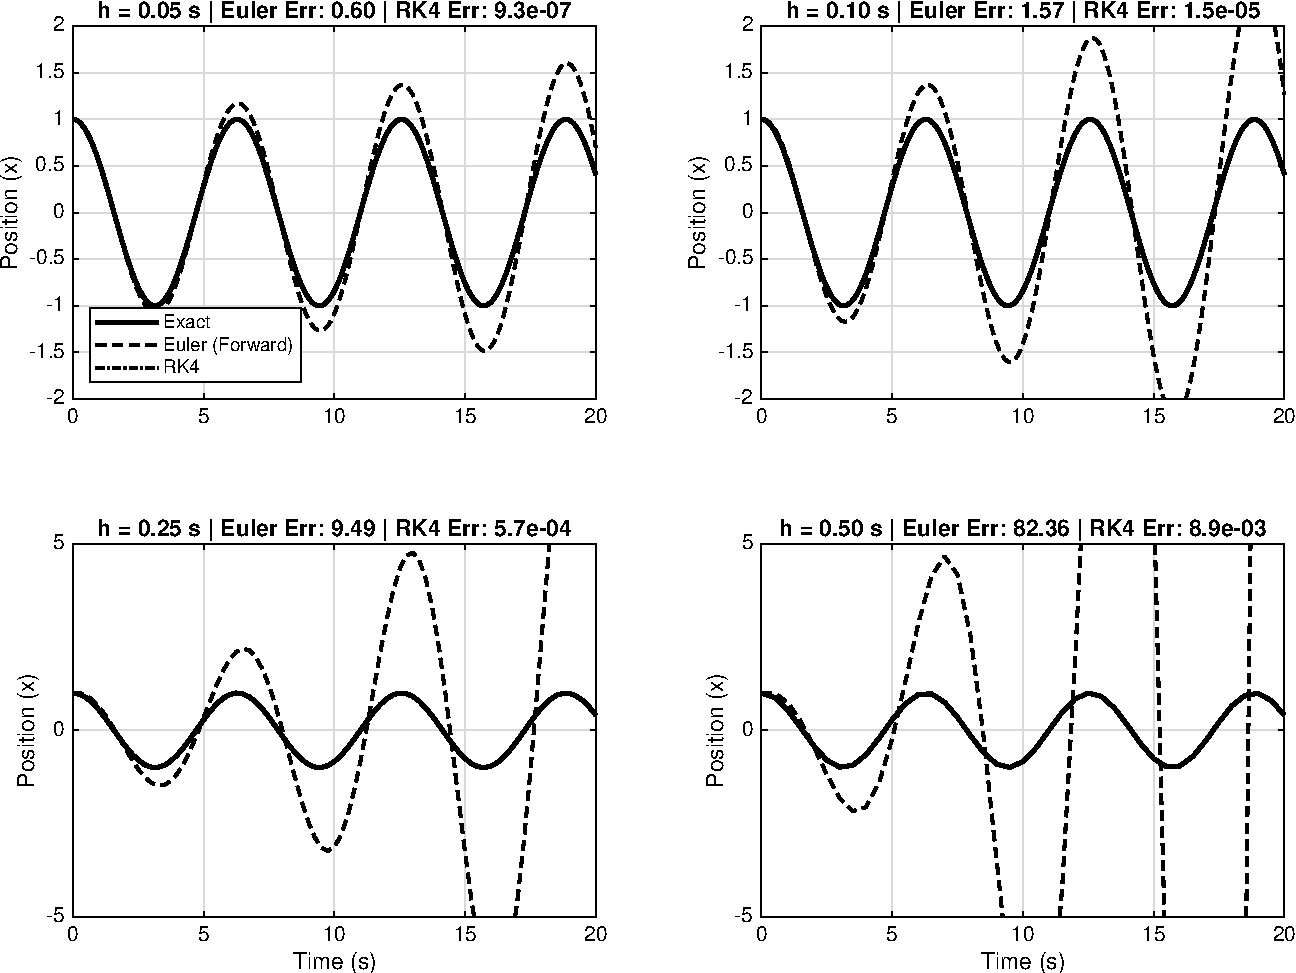
\includegraphics[width=1\linewidth]{Figures/RK4_vs_euler.pdf}
\caption{Comparison of numerical integration accuracy for an undamped harmonic oscillator ($\ddot{p} + p = 0$) across increasing time steps $h \in \{0.05, 0.10, 0.25, 0.50\}$ seconds. For this system (purely imaginary eigenvalues), the \textbf{Forward Euler} method (red dashed) is numerically unstable; it introduces artificial energy into the simulation, causing the amplitude to grow unbounded as time progresses. This error scales linearly with $h$. In contrast, the \textbf{Runge--Kutta 4 (RK4)} method (blue dash-dot) maintains high fidelity to the \textbf{Exact} solution (solid gray), preserving stability even at the coarsest time step of $h=0.50$\,s.}
	\label{fig:integrator_comparison}
\end{figure}


\section{Stability of Discrete-Time Systems}

The dynamics of a discrete-time system can be viewed as an iterated map:
\[
{x}_{k+1} = {f}_d({x}_k).
\]
An equilibrium point ${x}^*$ satisfies ${f}_d({x}^*) = {x}^*$. To analyse the local stability of ${x}^*$, we linearise the dynamics around this point:
\[
\delta {x}_{k+1} \approx {A}_d \delta {x}_k,
\quad \text{where} \quad 
{A}_d = \left. \frac{\partial {f}_d}{\partial {x}} \right|_{{x} = {x}^*}.
\]

\begin{alertbox}{Discrete-Time Stability Condition}
 The equilibrium point ${x}^*$ is (locally) asymptotically stable if and only if all eigenvalues of ${A}_d$ lie strictly inside the unit circle in the complex plane:
	\begin{equation*}
		|\lambda_i({A}_d)| < 1 \quad \forall i.
	\end{equation*}
\end{alertbox}

For linear systems ${x}_{k+1} = {A}_d {x}_k$, this condition is both necessary and sufficient.

\subsection{Geometric Interpretation: The Unit Circle}

Unlike continuous-time systems, where stability is defined by the Left Half Plane (LHP), discrete-time stability is determined by the \textbf{Unit Circle}. The mapping between the two domains is governed by the relation $z = e^{sh}$, where $h$ is the sampling time. Figure~\ref{fig:unit_circle} shows an unstable system having 4 eigenvalues. 

\begin{itemize}
	\item \textbf{Stable:} Eigenvalues lie strictly \emph{inside} the unit circle ($|\lambda| < 1$). The state vector decays to zero.
	\item \textbf{Unstable:} At least one eigenvalue lies \emph{outside} the unit circle ($|\lambda| > 1$). The state vector grows unbounded.
	\item \textbf{Marginally Stable:} Eigenvalues lie \emph{on} the unit circle ($|\lambda| = 1$). The system may oscillate or remain constant, but does not decay.
\end{itemize}

\begin{figure}[h]
	\centering
	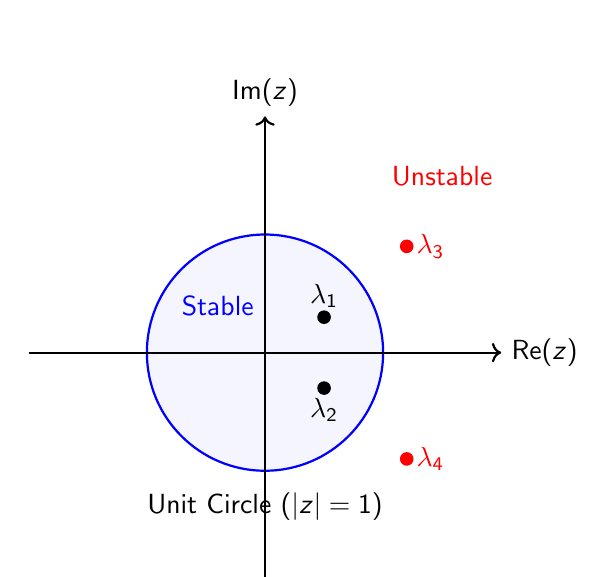
\begin{tikzpicture}[scale=1.5]		
		% Unit Circle
		\draw[thick, blue, fill=blue!4] (0,0) circle (1cm);
		\node[blue] at (-0.4,0.4) {Stable};
		
		% Labels
		\node [red] at (1.5, 1.5) {Unstable};
		
		% Roots examples
		\filldraw[black] (0.5, 0.3) circle (1.5pt) node[above] {$\lambda_1$};
		\filldraw[black] (0.5, -0.3) circle (1.5pt) node[below] {$\lambda_2$};
		\filldraw[red] (1.2, 0.9) circle (1.5pt) node[right] {$\lambda_3$};
		\filldraw[red] (1.2, -0.9) circle (1.5pt) node[right] {$\lambda_4$};
		
		% Annotation
		\node[anchor=north] at (0,-1.1) {Unit Circle ($|z|=1$)};
		\draw[->, thick] (-2,0) -- (2,0) node[right] {Re($z$)};
		\draw[->, thick] (0,-2) -- (0,2) node[above] {Im($z$)};
	\end{tikzpicture}
	\caption{Stability in the Z-plane. For the system to be stable, all eigenvalues (poles) must reside within the shaded blue region. Blue eigenvalues are stable whereas red ones are unstable. Therefore the system having these eigenvalues is unstable.}
	\label{fig:unit_circle}
\end{figure}

\subsection{Lyapunov Stability and the Stein Equation}

While eigenvalue analysis is useful for linear analysis, a more general approach—fundamental to optimal control—is the \textbf{Lyapunov method}. Instead of looking at roots of a polynomial, we look at the system's "energy".

For a linear discrete-time system $x_{k+1} = A x_k$, let us define a quadratic energy candidate function:
\begin{equation}
	V(x_k) = x_k^\top P x_k
\end{equation}
where $P$ is a symmetric, positive definite matrix ($P \succ 0$). For the system to be stable, this energy must decrease at every time step ($V(x_{k+1}) < V(x_k)$).

Substituting the dynamics into the energy difference yields:
\begin{align*}
	V(x_{k+1}) - V(x_k) &= x_{k+1}^\top P x_{k+1} - x_k^\top P x_k \\
	&= (A x_k)^\top P (A x_k) - x_k^\top P x_k \\
	&= x_k^\top (A^\top P A - P) x_k
\end{align*}
For the energy to decrease strictly, the term in the brackets must be negative definite. This leads to the \textbf{Discrete Lyapunov Equation}, also known as the \textit{Stein Equation}.

\begin{alertbox}{Lyapunov Stability Theorem}
	The discrete-time linear system $x_{k+1} = A x_k$ is asymptotically stable if and only if, for any given positive definite matrix $Q \succ 0$, there exists a unique positive definite matrix $P \succ 0$ satisfying:
	\begin{equation*}
		A^\top P A - P = -Q
	\end{equation*}
\end{alertbox}

\begin{notebox}{Connection to LQR}
	This equation is not just a stability check; it is the foundation of the Linear Quadratic Regulator. In LQR, we essentially look for a control law that shapes the matrix $A_{cl} = (A-BK)$ such that this energy-decrease condition is satisfied optimally.
\end{notebox}

\begin{notebox}{Further reading}
Standard references for state-space modelling and discretisation include \citet{Ogata2010} and \citet{Franklin2015}. The reader seeking a deeper treatment of continuous-to-discrete conversion methods is referred to these texts.
\end{notebox}

\section*{Exercises}

\begin{enumerate}

\item \textbf{Transfer Function to State-Space Conversion.}
A system is described by the transfer function
\[
G(s) = \frac{s + 3}{s^3 + 4s^2 + 6s + 4}.
\]
\begin{enumerate}
	\item[(a)] Convert $G(s)$ into a continuous-time state-space representation $\dot{x} = Ax + Bu$, $y = Cx + Du$ using the controllable canonical form. Clearly state the matrices $A$, $B$, $C$, and $D$.
	\item[(b)] Verify that $D = 0$ and explain, in terms of the degrees of numerator and denominator, why this is the case.
\end{enumerate}

\item \textbf{Matrix Exponential Computation.}
Consider the continuous-time system $\dot{x} = Ax$ with
\[
A = \begin{bmatrix} 0 & 1 \\ 0 & 0 \end{bmatrix}.
\]
\begin{enumerate}
	\item[(a)] Using the Taylor series definition $e^{M} = I + M + \frac{1}{2!}M^2 + \frac{1}{3!}M^3 + \cdots$, compute $e^{Ah}$ analytically by first evaluating $A^2$, $A^3$, etc.
	\item[(b)] For the initial condition $x(0) = [\,1 \;\; 2\,]^\top$, write the closed-form expression for $x(t)$.
	\item[(c)] Now let $A = \begin{bmatrix} -1 & 0 \\ 0 & -3 \end{bmatrix}$. Compute $e^{Ah}$ and comment on how the diagonal structure simplifies the computation.
\end{enumerate}

\item \textbf{Zero-Order Hold Discretisation.}
A mass--spring--damper system with mass $m = 1\,\text{kg}$, damping coefficient $c = 2\,\text{Ns/m}$, and spring stiffness $k = 5\,\text{N/m}$ has the continuous-time state-space model
\[
\dot{x} = \begin{bmatrix} 0 & 1 \\ -5 & -2 \end{bmatrix} x + \begin{bmatrix} 0 \\ 1 \end{bmatrix} u, \qquad y = \begin{bmatrix} 1 & 0 \end{bmatrix} x.
\]
\begin{enumerate}
	\item[(a)] Form the augmented matrix
	$T = \begin{bmatrix} A & B \\ 0 & 0 \end{bmatrix}$
	and explain why computing $e^{Th}$ yields the exact discrete-time matrices $A_d$ and $B_d$ under a ZOH assumption.
	\item[(b)] Using MATLAB (or by hand for bonus practice), compute $A_d$ and $B_d$ for a sampling time $h = 0.1\,\text{s}$.
	\item[(c)] Write the resulting discrete-time state-space model $x_{k+1} = A_d x_k + B_d u_k$ and the output equation $y_k = C_d x_k$.
\end{enumerate}

\item \textbf{Deviation Variables and Linearisation.}
Consider the nonlinear system describing a continuously stirred tank reactor (CSTR):
\[
\dot{x}_1 = -x_1 + D_a(1 - x_1)\exp\!\left(\frac{x_2}{1 + x_2/\gamma}\right), \qquad
\dot{x}_2 = -(1+\beta)x_2 + D_a B(1 - x_1)\exp\!\left(\frac{x_2}{1 + x_2/\gamma}\right) + \beta\, u,
\]
where $x_1$ is the dimensionless concentration, $x_2$ is the dimensionless temperature, $u$ is the coolant temperature, and $D_a$, $B$, $\beta$, $\gamma$ are positive parameters.
\begin{enumerate}
	\item[(a)] Suppose an equilibrium $(x_{1,e},\, x_{2,e},\, u_e)$ has been found numerically. Write the general expressions for the Jacobian matrices
	$A = \dfrac{\partial f}{\partial x}\Big|_{(x_e, u_e)}$ and $B = \dfrac{\partial f}{\partial u}\Big|_{(x_e, u_e)}$.
	\item[(b)] Define the deviation variables $\tilde{x} = x - x_e$ and $\tilde{u} = u - u_e$, and write the linearised model $\dot{\tilde{x}} = A\tilde{x} + B\tilde{u}$.
	\item[(c)] Explain why the linearised model is only valid in a neighbourhood of $(x_e, u_e)$ and what happens to its accuracy as $\|\tilde{x}\|$ and $\|\tilde{u}\|$ increase.
\end{enumerate}

\item \textbf{Eigenvalue Analysis for Stability.}
Consider the discrete-time system $x_{k+1} = A_d x_k$ with
\[
A_d = \begin{bmatrix} 0.5 & 0.3 \\ -0.2 & 0.4 \end{bmatrix}.
\]
\begin{enumerate}
	\item[(a)] Compute the eigenvalues of $A_d$ by solving $\det(A_d - \lambda I) = 0$.
	\item[(b)] Determine whether the system is asymptotically stable by checking the discrete-time stability condition $|\lambda_i(A_d)| < 1$ for all $i$.
	\item[(c)] Now consider the modified system matrix
	$A_d' = \begin{bmatrix} 0.8 & 0.6 \\ -0.6 & 0.8 \end{bmatrix}$.
	Compute the eigenvalues of $A_d'$ and determine whether the system is stable, unstable, or marginally stable. Sketch the location of the eigenvalues relative to the unit circle in the $z$-plane.
\end{enumerate}

\item \textbf{From Physics to Discrete-Time Model (Combined Exercise).}
An electrical circuit consists of a single resistor $R$ in series with an inductor $L$, driven by a voltage source $v_i(t)$. The current through the inductor is $i_L(t)$.
\begin{enumerate}
	\item[(a)] Using Kirchhoff's voltage law, derive the first-order differential equation governing $i_L(t)$.
	\item[(b)] Write the continuous-time state-space model with $x = i_L$ and $u = v_i$, identifying the scalars $A$, $B$, $C$, and $D$ (assume the output is the inductor current).
	\item[(c)] Compute the exact ZOH discrete-time model $x_{k+1} = A_d x_k + B_d u_k$ analytically. \textit{Hint:} For a scalar system, $A_d = e^{Ah}$ and $B_d = \int_0^h e^{A\tau}\,d\tau \cdot B$.
	\item[(d)] Compute the eigenvalue of $A_d$ and determine the condition on $R$, $L$, and $h$ for which the discrete-time system is stable.
\end{enumerate}

\end{enumerate}

	%%%%%%%%%%%%%%%%%%%%%%%%%%%%%%%%%%%%%%%%%%%%%%%%%%%%%%%%%%%%%%%%%%%%%%%%%
%                   CHAPTER 4: CONTROLLABILITY                          %
%%%%%%%%%%%%%%%%%%%%%%%%%%%%%%%%%%%%%%%%%%%%%%%%%%%%%%%%%%%%%%%%%%%%%%%%%

\chapter{Controllability \& Observability}
\label{chap:controllability}


Now that we have established the state-space modelling framework (Chapter~\ref{chap:statespace}), we turn to two structural questions that determine whether a control or estimation design is even possible.

In previous chapters, we focused on the machinery of optimisation—how to select the \textit{best} input to minimise a cost function. However, before asking "what is the optimal trajectory?", we must answer a more fundamental question: "does a valid trajectory exist?"

This chapter introduces the twin structural properties of \textbf{controllability} and \textbf{observability}. These concepts define the physical limitations of what a control system can achieve, regardless of the sophistication of the algorithm used.

\begin{itemize}
	\item \textbf{Controllability} answers the question of \textit{actuation}: Is it possible to steer the system from its current state to any desired target state using the available inputs? If a system is unreachable, no amount of mathematical optimisation can force it to the target.
	
	\item \textbf{Observability} answers the question of \textit{sensing}: Is it possible to reconstruct the full internal state of the system solely by monitoring the inputs and outputs? Since MPC and LQR typically require full state feedback ($x_k$), observability is the prerequisite for designing the estimators (such as Kalman Filters) required to implement these controllers in reality.
\end{itemize}

For modern control strategies like Model Predictive Control, these are not merely theoretical curiosities; they are the necessary existence conditions. If a system lacks these properties, the optimisation problem may be ill-posed, leading to controllers that are either unstable or physically incapable of meeting their objectives.

\section{Controllability}

The fundamental question of controllability is: given the dynamics $x_{k+1} = A x_k + B u_k$, do the actuators (represented by matrix $B$) possess sufficient authority over the system states (governed by matrix $A$) to drive the system to a specific target?

Consider a trivial example where the matrix $B$ is all zeros. In such a case, the control input $u_k$ has no effect on the state evolution, rendering us powerless to change the trajectory. While this is an extreme case, a system can be uncontrollable even with non-zero actuators if their influence is geometrically restricted to a specific subspace of the state space.

\begin{defnbox}{Definition: Controllability}
A system is \emph{controllable} if, for any initial state $x_0$ and any target state $x_N$, there exists a finite sequence of control inputs that drives the system from $x_0$ to $x_N$.
\end{defnbox}

\subsection{Derivation of the Rank Condition}

For Linear Time-Invariant (LTI) systems where the state vector is $x_k \in \mathbb R^n$, we can derive a simple algebraic test for controllability. We begin by expanding the discrete-time dynamics to express the state $x_N$ as a function of the initial state $x_0$ and the control history.

Starting from $k=0$ and substituting recursively:
\begin{align*}
	x_1 &= A x_0 + B u_0 \\
	x_2 &= A x_1 + B u_1 = A(A x_0 + B u_0) + B u_1 = A^2 x_0 + AB u_0 + B u_1 \\
	&\vdots \\
	x_N &= A^N x_0 + \sum_{i=0}^{N-1} A^{N-1-i} B u_i
\end{align*}

We can rewrite this summation in a compact matrix-vector form. By collecting all control inputs into a stacked vector $\mathcal{U}$, we obtain:
\[
x_N - A^N x_0 = 
\underbrace{\begin{bmatrix} B & AB & A^2 B & \cdots & A^{N-1} B \end{bmatrix}}_{\mathcal{C}_N}
\underbrace{\begin{bmatrix} u_{N-1} \\ u_{N-2} \\ \vdots \\ u_0 \end{bmatrix}}_{\mathcal{U}}
\]
This equation is a linear system of the form ${b} = \mathcal{C}_N\, \mathcal{U}$. The controllability problem reduces to a linear algebra problem: 

\begin{alertbox}{Question}
Does a solution $\mathcal{U}$ exist for any desired vector ${b} = x_N - A^N x_0$?
\end{alertbox}
For a solution to exist for \emph{any} target state in the $n$-dimensional state space, the matrix $\mathcal{C}_N$ must span $\mathbb{R}^n$. This requires $\mathcal{C}_N$ to have full row rank. 

While this matrix grows with the horizon $N$, the \textbf{Cayley-Hamilton Theorem} tells us that any matrix power $A^k$ for $k \ge n$ can be written as a linear combination of lower powers ($I, \dots, A^{n-1}$). Consequently, adding columns beyond $A^{n-1}B$ provides no new linearly independent directions.
The Cayley-Hamilton Theorem states that every square matrix satisfies its own characteristic equation; as a consequence, $A^n$ (and all higher powers) can be expressed as a linear combination of $I, A, \dots, A^{n-1}$.
We can therefore define the standard \textbf{Controllability Matrix} $\mathcal{C}$ using only $n$ blocks.

\begin{equation*}
	\mathcal{C} = \begin{bmatrix} B & AB & A^2 B & \cdots & A^{n-1} B \end{bmatrix}
\end{equation*}

\begin{alertbox}{Theorem: The Kalman Rank Condition}
	Consider an LTI system with state dimension $n$. The system pair $(A, B)$ is controllable if and only if the \textbf{controllability matrix} $\mathcal{C}$ has full rank:
	\begin{equation*}
		\text{rank}(\mathcal{C}) = n
	\end{equation*}
	where the matrix is constructed from the system matrices as:
	\begin{equation*}
		\mathcal{C} = \begin{bmatrix} B & AB & A^2B & \cdots & A^{n-1}B \end{bmatrix}
	\end{equation*}
	\textbf{Interpretation:} If this condition holds, the columns of $\mathcal{C}$ span the entire state space $\mathbb{R}^n$. This guarantees that there is no "hidden" subspace where the state can get stuck; the input $u$ has the authority to steer the state vector anywhere in the $n$-dimensional space.
\end{alertbox}

\begin{figure}[H]
	\centering
	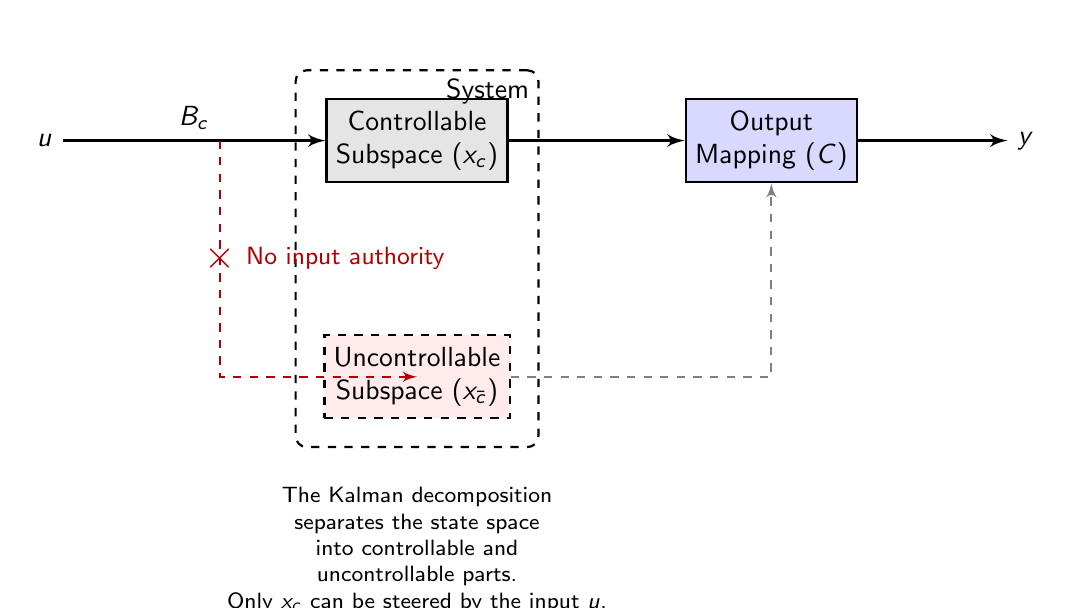
\begin{tikzpicture}[auto, >=latex', thick]
		% Define styles
		\tikzstyle{block} = [draw, rectangle, fill=gray!20, minimum height=3em, minimum width=6em, align=center]
		\tikzstyle{dashedblock} = [draw, dashed, rectangle, fill=red!8, minimum height=3em, minimum width=6em, align=center]
		\tikzstyle{line} = [draw, ->]
		\tikzstyle{bigbox} = [draw, dashed, rounded corners, inner sep=10pt]

		% Input
		\node [coordinate] (input) at (-1.5, 0) {};
		\node [left] at (input) {$u$};

		% Controllable subspace block
		\node [block] (controllable) at (3, 0) {Controllable\\Subspace ($x_c$)};

		% Uncontrollable subspace block
		\node [dashedblock] (uncontrollable) at (3, -3) {Uncontrollable\\Subspace ($x_{\bar{c}}$)};

		% Summing point / output
		\node [block, fill=blue!15] (output_map) at (7.5, 0) {Output\\Mapping ($C$)};

		% Output
		\node [coordinate] (output) at (10.5, 0) {};
		\node [right] at (output) {$y$};

		% System boundary
		\node [bigbox, fit=(controllable)(uncontrollable), label={[anchor=north east]north east:System}] (system) {};

		% Arrows
		\draw [line, line width=1.2pt] (input) -- node[above]{$B_c$} (controllable);
		\draw [line, line width=1.2pt] (controllable) -- (output_map);
		\draw [line, line width=1.2pt] (output_map) -- (output);

		% Dashed arrow from uncontrollable to output (it may still affect y)
		\draw [line, dashed, gray] (uncontrollable) -| (output_map);

		% Crossed-out arrow to show u does NOT reach uncontrollable subspace
		\draw [line, dashed, red!70!black] (0.5, 0) -- (0.5, -3) -- (controllable |- uncontrollable.west);
		\node [red!70!black, font=\Large\bfseries] at (0.5, -1.5) {$\times$};
		\node [red!70!black, font=\small, right] at (0.7, -1.5) {No input authority};

		% Annotation
		\node [font=\footnotesize, text width=5cm, align=center] at (3, -5.2) {The Kalman decomposition separates the state space\\into controllable and uncontrollable parts.\\Only $x_c$ can be steered by the input $u$.};

	\end{tikzpicture}
	\caption{Controllability decomposition of a linear system. The input $u$ drives only the controllable subspace $x_c$. The uncontrollable subspace $x_{\bar{c}}$ evolves independently of $u$ and cannot be steered by any control action. Both subspaces may contribute to the output $y$.}
	\label{fig:controllability_decomposition}
\end{figure}

\subsection{Controllability in MATLAB}

Let us verify this condition for a discrete-time double integrator system. While we could construct the matrix manually, the best practice is to use the MATLAB Control System Toolbox function \texttt{ctrb}. This ensures the method generalizes correctly to higher-dimensional systems.

\begin{lstlisting}[language=Matlab, caption={MATLAB script to check controllability using the \texttt{ctrb} command.}, label={lst:matlab_controllability}]
	% 1. Define the discrete-time double integrator
	h = 0.1;               % Sampling time
	A = [1, h; 
			0, 1];            
	
	B = [0.5*h^2; 
			h];               
	
	n = size(A, 1);        
	
	% 2. Compute Controllability Matrix
	Co = ctrb(A, B);
	
	% 3. Check Rank Condition
	rank_Co = rank(Co);
	
	fprintf('State Dimension n = %d\n', n);
	fprintf('Rank of Co      = %d\n', rank_Co);

\end{lstlisting}

\textbf{Results}\\

Since the rank of the controllability matrix (2) equals the number of states (2), the system is controllable. This mathematically guarantees that an input sequence exists to drive the robot from any initial position and velocity to any target state (assuming no actuator saturation), satisfying the necessary condition for LQR design which will be covered in the next chapter.

\section{Observability}

While controllability deals with the active problem of steering the state $x$ using the input $u$, \textbf{observability} addresses the passive inverse problem: can we reconstruct the internal state $x(t)$ solely by monitoring the system's input $u(t)$ and output $y(t)$?

This concept is fundamental for practical MPC implementation. Most advanced control strategies (including MPC and LQR) are \textit{state-feedback} controllers, meaning they calculate the optimal input $u = -Kx$ based on the full state vector. However, in reality, we rarely measure every state variable directly due to sensor costs or physical impossibility. Instead, we measure a subset $y = Cx$ and use a mathematical algorithm known as a \textit{State Observer} (e.g., a Kalman Filter) to estimate the missing variables. Observability is the mathematical guarantee that this estimation is possible.

\begin{defnbox}{Observability}
	A linear system is defined as \textbf{observable} if the initial state $x(t_0)$ can be uniquely determined from the knowledge of the system input $u(t)$ and output $y(t)$ over a finite time interval $t_0 \leq t \leq t_1$. 
	
	If a system is \textbf{unobservable}, there exists at least one "hidden" mode inside the system that does not affect the output $y(t)$. Consequently, the controller acts "blindly" with respect to this mode, which can lead to undetected instability.
\end{defnbox}

\subsection{The Observability Matrix}
For an LTI system defined by matrices $A$ (dynamics) and $C$ (measurement), observability is a structural property of the pair $(A, C)$. It determines whether the information from the internal states propagates to the output.

To test for this property, we construct the \textbf{Observability Matrix}, denoted by $\mathcal{O}$:
\begin{equation*}
	\mathcal{O} = 
	\begin{bmatrix}
		C \\
		CA \\
		CA^2 \\
		\vdots \\
		CA^{n-1}
	\end{bmatrix}
\end{equation*}
Note that $\mathcal{O}$ is a matrix of dimension $(n \cdot p) \times n$, where $n$ is the number of states and $p$ is the number of outputs.

\begin{notebox}{Kalman Rank Condition for Observability}
	An LTI system is fully observable if and only if the observability matrix has \textbf{full column rank}:
	\begin{equation*}
		\text{rank}(\mathcal{O}) = n
	\end{equation*}
	If the rank is less than $n$, the system is unobservable, and the \emph{unobservable states} correspond to the null space of $\mathcal{O}$.
\end{notebox}

\begin{examplebox}{Unobservable Systems}
Consider a simple 2-state system where the dynamics are decoupled, and we only measure the first state:
\begin{align*}
	\dot{x} &= \begin{bmatrix} -1 & 0 \\ 0 & -2 \end{bmatrix} x + \begin{bmatrix} 1 \\ 1 \end{bmatrix} u \\
	y &= \underbrace{\begin{bmatrix} 1 & 0 \end{bmatrix}}_{C} x
\end{align*}
Here, $x_1$ decays with time constant 1, and $x_2$ decays with time constant 0.5. The sensor $y$ measures $x_1$ perfectly.

Let us check the Observability Matrix $\mathcal{O}$:
\begin{equation*}
	\mathcal{O} = \begin{bmatrix} C \\ CA \end{bmatrix} 
	= \begin{bmatrix} 
		1 & 0 \\ 
		(1)(-1) + (0)(0) & (1)(0) + (0)(-2) 
	\end{bmatrix}
	= \begin{bmatrix} 
		1 & 0 \\ 
		-1 & 0 
	\end{bmatrix}
\end{equation*}
The second column is entirely zero. The rank of this matrix is 1 (which is less than $n=2$). 

\textbf{Interpretation:} The sensor output $y$ is mathematically disconnected from state $x_2$. No matter how long we record the data, we can never know the value of $x_2$. If $x_2$ were unstable (e.g., a positive eigenvalue), the system would explode, and the controller would be unaware until the machine physically failed.
\end{examplebox}

\begin{examplebox}{Controllability of a Three-State System}
Consider a three-state system with the following sparse matrices:
\begin{equation*}
	A = \begin{bmatrix} 0 & 1 & 0 \\ 0 & 0 & 1 \\ 0 & 0 & 0 \end{bmatrix}, \qquad
	B = \begin{bmatrix} 0 \\ 0 \\ 1 \end{bmatrix}
\end{equation*}
This system represents a \textit{triple integrator} (e.g., a frictionless mass where the input is a jerk signal --- the rate of change of acceleration). The state vector is $x = \begin{bmatrix} \text{position} & \text{velocity} & \text{acceleration} \end{bmatrix}^\top$.

Since $n = 3$, the controllability matrix requires three blocks: $\mathcal{C} = \begin{bmatrix} B & AB & A^2 B \end{bmatrix}$.

\textbf{Step 1:} Compute $AB$:
\begin{equation*}
	AB = \begin{bmatrix} 0 & 1 & 0 \\ 0 & 0 & 1 \\ 0 & 0 & 0 \end{bmatrix}
	\begin{bmatrix} 0 \\ 0 \\ 1 \end{bmatrix}
	= \begin{bmatrix} 0 \\ 1 \\ 0 \end{bmatrix}
\end{equation*}

\textbf{Step 2:} Compute $A^2 B$:
\begin{equation*}
	A^2 B = A(AB) = \begin{bmatrix} 0 & 1 & 0 \\ 0 & 0 & 1 \\ 0 & 0 & 0 \end{bmatrix}
	\begin{bmatrix} 0 \\ 1 \\ 0 \end{bmatrix}
	= \begin{bmatrix} 1 \\ 0 \\ 0 \end{bmatrix}
\end{equation*}

\textbf{Step 3:} Assemble the controllability matrix:
\begin{equation*}
	\mathcal{C} = \begin{bmatrix} B & AB & A^2 B \end{bmatrix}
	= \begin{bmatrix} 0 & 0 & 1 \\ 0 & 1 & 0 \\ 1 & 0 & 0 \end{bmatrix}
\end{equation*}

\textbf{Step 4:} Determine the rank. The matrix $\mathcal{C}$ is a permutation matrix (each row and each column contains exactly one non-zero entry). Its determinant is:
\begin{equation*}
	\det(\mathcal{C}) = 0 \cdot (0 \cdot 0 - 0 \cdot 0) - 0 \cdot (0 \cdot 0 - 1 \cdot 0) + 1 \cdot (0 \cdot 0 - 1 \cdot 1) = -1 \neq 0
\end{equation*}
Therefore $\text{rank}(\mathcal{C}) = 3 = n$.

\textbf{Interpretation:} The system is fully controllable. Despite the input $u$ entering only the third state equation directly, its effect propagates through the chain of integrators: after one time step, the input influences $x_3$; after two steps, it reaches $x_2$; and after three steps, it reaches $x_1$. The single actuator has full authority over all three states, which is a characteristic property of systems in \textit{controllable canonical form}.
\end{examplebox}

\begin{examplebox}{Observable System: Adding a Second Sensor}
Consider the same 2-state system from the previous unobservable example, but suppose we replace the sensor with one that measures a \textit{combination} of both states:
\begin{align*}
	\dot{x} &= \begin{bmatrix} -1 & 0 \\ 0 & -2 \end{bmatrix} x + \begin{bmatrix} 1 \\ 1 \end{bmatrix} u \\
	y &= \underbrace{\begin{bmatrix} 1 & 1 \end{bmatrix}}_{C} x
\end{align*}
The $A$ matrix is identical to the unobservable case. The only change is that $C = \begin{bmatrix} 1 & 1 \end{bmatrix}$ instead of $\begin{bmatrix} 1 & 0 \end{bmatrix}$. Physically, this sensor now measures $y = x_1 + x_2$, coupling both states into the output.

Let us construct the observability matrix $\mathcal{O}$:

\textbf{Step 1:} Compute $CA$:
\begin{equation*}
	CA = \begin{bmatrix} 1 & 1 \end{bmatrix}
	\begin{bmatrix} -1 & 0 \\ 0 & -2 \end{bmatrix}
	= \begin{bmatrix} -1 & -2 \end{bmatrix}
\end{equation*}

\textbf{Step 2:} Assemble the observability matrix:
\begin{equation*}
	\mathcal{O} = \begin{bmatrix} C \\ CA \end{bmatrix}
	= \begin{bmatrix} 1 & 1 \\ -1 & -2 \end{bmatrix}
\end{equation*}

\textbf{Step 3:} Check the rank. The determinant is:
\begin{equation*}
	\det(\mathcal{O}) = (1)(-2) - (1)(-1) = -2 + 1 = -1 \neq 0
\end{equation*}
Therefore $\text{rank}(\mathcal{O}) = 2 = n$.

\textbf{Interpretation:} The system is now fully observable. By measuring a linear combination of both states rather than a single state in isolation, the sensor output $y = x_1 + x_2$ contains information about both modes. Because the two modes decay at different rates ($\lambda_1 = -1$ and $\lambda_2 = -2$), the observer can separate their individual contributions from the mixed signal over time. This example demonstrates that observability is a property of the \textit{pair} $(A, C)$: the same dynamics can be observable or unobservable depending entirely on the sensor configuration.
\end{examplebox}

\subsection{Derivation of the Rank Condition}

We can derive the observability condition intuitively by considering a Discrete-Time LTI system. Our objective is simple: given a sequence of measurements $y_0, y_1, \dots$, can we mathematically calculate the initial state vector $x_0$?

\subsubsection*{Step 1: Isolating the Unforced Response}
The general output equation is:
\begin{equation*}
	y_k = C A^k x_0 + \sum_{j=0}^{k-1} C A^{k-1-j} B u_j + D u_k
\end{equation*}
Based on the {Principle of Superposition}, the output consists of two parts: the \textit{free response} (dependent only on initial conditions) and the \textit{forced response} (dependent on inputs). Since the inputs $u_k$ are known, we can calculate the forced response and subtract it from the measurement. Thus, without loss of generality, we treat the problem as solving for $x_0$ in the unforced system:
\begin{align*}
	x_{k+1} &= A x_k \\
	y_k &= C x_k
\end{align*}

\subsubsection*{Step 2: Stacking the Measurements}
Let us observe the system for $n$ time steps (where $n$ is the dimension of the state vector) and write the output at each step in terms of the initial state $x_0$:
\begin{align*}
	k=0: & \quad y_0 = C x_0 \\
	k=1: & \quad y_1 = C x_1 = C (A x_0) = CA x_0 \\
	k=2: & \quad y_2 = C x_2 = C (A^2 x_0) = CA^2 x_0 \\
	& \quad \vdots \\
	k=n-1: & \quad y_{n-1} = C A^{n-1} x_0
\end{align*}

\subsubsection*{Step 3: The Linear System of Equations}
We can stack these individual equations into a single large matrix equation $Y = \mathcal{O} x_0$:
\begin{equation*}
	\underbrace{\begin{bmatrix} y_0 \\ y_1 \\ \vdots \\ y_{n-1} \end{bmatrix}}_{{Y}}
	=
	\underbrace{\begin{bmatrix} C \\ CA \\ \vdots \\ CA^{n-1} \end{bmatrix}}_{\mathcal{O}}
	x_0
\end{equation*}

Here:
\begin{itemize}
	\item ${Y}$ is the vector of collected measurements (known).
	\item $\mathcal{O}$ is the \textbf{Observability Matrix} (known).
	\item $x_0$ is the state vector we wish to find (unknown).
\end{itemize}

\subsubsection*{Step 4: The Invertibility Condition}
This is a standard linear algebra problem of the form $Ax = b$. We have $n$ unknowns (the elements of $x_0$). To find a \textbf{unique} solution for $x_0$, the matrix $\mathcal{O}$ must provide enough independent equations to constrain the solution fully.

Mathematically, this requires that the mapping be invertible (specifically, left-invertible). This is only possible if the columns of $\mathcal{O}$ are linearly independent.

\begin{summarybox}{The Rank Test}
	A system is observable if and only if the Observability Matrix has full rank:
	\begin{equation*}
		\text{rank}(\mathcal{O}) = n
	\end{equation*}
	If this holds, we can uniquely solve for the state via the left pseudo-inverse:
	\[ x_0 = (\mathcal{O}^\top \mathcal{O})^{-1} \mathcal{O}^\top {Y} \]
\end{summarybox}

\textit{Note:} One might ask, "Why stop at $n-1$?" According to the \textbf{Cayley-Hamilton Theorem}, any matrix power $A^k$ for $k \ge n$ can be written as a linear combination of lower powers ($I, A, \dots, A^{n-1}$). Therefore, taking more measurements beyond $k=n-1$ adds rows to $\mathcal{O}$ that are linearly dependent on previous rows, providing no new information for determining the rank.

\subsection{Observability in MATLAB}

To demonstrate the physical meaning of observability, we analyse the double integrator model (position and velocity) under two different sensor configurations:
\begin{enumerate}
	\item \textbf{Position Sensor ($y=x_1$):} We measure position. Can we infer velocity? Intuitively yes, by observing the change in position over time.
	\item \textbf{Velocity Sensor ($y=x_2$):} We measure velocity. Can we infer position? Intuitively no, because we do not know the starting integration constant.
\end{enumerate}

\begin{lstlisting}[language=Matlab, caption={MATLAB script comparing two sensor configurations.}, label={lst:matlab_observability}]

	h = 0.1;
	A = [1, h; 
			0, 1];
	n = size(A, 1);
	
	C1 = [1, 0]; % We measure the first state
	
	Ob1 = obsv(A, C1);
	rank_Ob1 = rank(Ob1);
	
	C2 = [0, 1]; % We measure the second state
	
	Ob2 = obsv(A, C2);
	rank_Ob2 = rank(Ob2);
	
\end{lstlisting}

\textbf{Results:}\\

In Case 1, the matrix $\mathcal{O}$ has rank 2, meaning the rows are linearly independent; information about both states is present in the output history. In Case 2, the matrix has rank 1 (identical rows). The "position" mode is unobservable. If we only measure speed, the robot's absolute position is mathematically impossible to reconstruct.

\begin{defnbox}{Stabilisability and Detectability}
A pair $(A, B)$ is \textbf{stabilisable} if every uncontrollable mode of $A$ is stable (i.e.\ has eigenvalue magnitude less than 1 in discrete time, or negative real part in continuous time). Equivalently, $(A, B)$ is stabilisable if there exists a feedback gain $K$ such that $A - BK$ is Schur stable.

A pair $(A, C)$ is \textbf{detectable} if every unobservable mode of $A$ is stable. Equivalently, $(A, C)$ is detectable if there exists an observer gain $L$ such that $A - LC$ is Schur stable.
\end{defnbox}

Stabilisability is required for the existence of a stabilising solution to the discrete algebraic Riccati equation (DARE), which provides the LQR gain (Chapter~5) and the terminal cost in MPC (Chapter~7). Detectability of $(A, C)$ is required for the convergence of the Kalman filter (Chapter~6). These weaker conditions replace full controllability and observability in most practical design procedures.

\section*{Exercises}

\begin{enumerate}

\item Consider the discrete-time system $(A,\,B)$ with
\[
A = \begin{bmatrix} 0 & 1 & 0 \\ 0 & 0 & 1 \\ -6 & -11 & -6 \end{bmatrix}, \qquad
B = \begin{bmatrix} 0 \\ 0 \\ 1 \end{bmatrix}.
\]
\begin{enumerate}
	\item Construct the controllability matrix $\mathcal{C} = \begin{bmatrix} B & AB & A^2 B \end{bmatrix}$.
	\item Compute $\text{rank}(\mathcal{C})$ and determine whether the system is controllable.
	\item Repeat the analysis for $B' = \begin{bmatrix} 1 \\ 0 \\ 0 \end{bmatrix}$ and comment on how the input coupling affects controllability.
\end{enumerate}

\item A discrete-time system is described by
\[
A = \begin{bmatrix} 1 & 0.1 \\ 0 & 1 \end{bmatrix}, \qquad
C = \begin{bmatrix} 1 & 0 \end{bmatrix}.
\]
\begin{enumerate}
	\item Construct the observability matrix $\mathcal{O}$ and verify that $\text{rank}(\mathcal{O}) = 2$.
	\item Now change the output matrix to $C' = \begin{bmatrix} 0 & 0 \end{bmatrix}$ (i.e.\ no sensor). What is the rank of the resulting observability matrix, and what does this imply physically?
	\item Suppose instead $C'' = \begin{bmatrix} 1 & 1 \end{bmatrix}$. Determine whether the system $(A,\,C'')$ is observable.
\end{enumerate}

\item The \textbf{Popov--Belevitch--Hautus (PBH) test} provides an eigenvalue-based criterion for controllability: the pair $(A,\,B)$ is controllable if and only if
\[
\text{rank}\!\begin{bmatrix} \lambda I - A & B \end{bmatrix} = n \quad \text{for every eigenvalue } \lambda \text{ of } A.
\]
Consider the system
\[
A = \begin{bmatrix} -1 & 0 \\ 0 & -3 \end{bmatrix}, \qquad
B = \begin{bmatrix} 1 \\ 0 \end{bmatrix}.
\]
\begin{enumerate}
	\item Find the eigenvalues of $A$.
	\item Apply the PBH test at each eigenvalue to determine which modes are controllable and which are uncontrollable.
	\item Verify your conclusion by computing the controllability matrix $\mathcal{C}$ and checking its rank.
\end{enumerate}

\item A continuous-time system has the state-space representation
\[
A = \begin{bmatrix} -2 & 0 \\ 0 & 0.5 \end{bmatrix}, \qquad
B = \begin{bmatrix} 1 \\ 0 \end{bmatrix}.
\]
\begin{enumerate}
	\item Show that the pair $(A,\,B)$ is \emph{not} controllable by computing $\text{rank}(\mathcal{C})$.
	\item Identify the uncontrollable mode. Is this mode stable or unstable?
	\item Based on your answer, determine whether the system is \emph{stabilisable}. Justify your reasoning using the definition given in this chapter: a system is stabilisable if all uncontrollable modes are stable.
	\item Now suppose the system matrix is changed to $A' = \begin{bmatrix} -2 & 0 \\ 0 & -0.5 \end{bmatrix}$ while $B$ remains the same. Is this modified system stabilisable? Why or why not?
\end{enumerate}

\item Consider the continuous-time system
\[
A = \begin{bmatrix} 0 & 1 \\ -2 & -3 \end{bmatrix}, \qquad
C = \begin{bmatrix} 1 & 0 \end{bmatrix}.
\]
A state observer (Luenberger observer) reconstructs the state via
\[
\dot{\hat{x}} = A \hat{x} + B u + L(y - C \hat{x}),
\]
where $L \in \mathbb{R}^{2 \times 1}$ is the observer gain. The estimation error $e = x - \hat{x}$ satisfies $\dot{e} = (A - LC)\,e$.
\begin{enumerate}
	\item Verify that the pair $(A,\,C)$ is observable.
	\item Suppose we wish the observer error dynamics to have eigenvalues at $\{-5,\, -6\}$. Determine the gain vector $L = \begin{bmatrix} l_1 \\ l_2 \end{bmatrix}$ such that the characteristic polynomial of $(A - LC)$ matches $(\lambda + 5)(\lambda + 6) = \lambda^2 + 11\lambda + 30$.
	\item Comment on how the choice of observer eigenvalues (relative to the open-loop eigenvalues of $A$) affects the speed of state estimation convergence.
\end{enumerate}

\end{enumerate}
	\part{Optimal Control and Optimal Estimation}



\chapter{LQR Design via Quadratic Programming}
\label{chap:lqr}

\begin{quote}
	\textit{``The linear variance-minimisation problem... constitutes the most complete and elegant part of optimal control theory.''} \\
	
	\hfill --- \textbf{Huibert Kwakernaak \& Raphael Sivan}, \textit{Linear Optimal Control Systems} (1972)
\end{quote}

In the preceding chapters, we focused on modelling dynamical systems and analysing their fundamental properties such as stability, controllability, and observability. We now transition from \textit{analysis} to \textit{synthesis}. How do we design a controller that not only stabilises a system but does so in the best possible way?

The Linear Quadratic Regulator (LQR) is a foundational result in optimal control theory. It provides a systematic method to trade off regulation performance against control effort. Traditionally, this problem is introduced via the algebraic Riccati equation—a recursive solution ideal for infinite-horizon unconstrained problems. However, to fully grasp Model Predictive Control (MPC), we must view LQR through a different lens.

In this chapter, we adopt a numerical optimisation perspective. Instead of solving the control problem recursively (time-step by time-step), we will formulate the entire trajectory optimisation as a single, large static task—specifically, a \textbf{Quadratic Programme (QP)}.

By "stacking" the predicted states and inputs into large vectors, we transform the dynamic control problem into a standard linear algebra problem. The required linear algebra background is reviewed in Appendix~\ref{app:linalg}. This "batch" approach not only provides a one-shot, exact solution but also establishes the essential mathematical framework required to incorporate physical constraints in the chapters that follow.

\section{Problem Formulation}

The discrete-time LQR problem aims to determine the optimal sequence of control inputs $u$ and the corresponding state trajectory $x$ that minimise a quadratic cost function. The optimisation is constrained by the linear evolution of the system, anchored by a known, fixed initial state $x_0$.

Mathematically, we define the decision variables as the sequence of inputs $\{u_0, \dots, u_{N-1}\}$ and the sequence of future states $\{x_1, \dots, x_N\}$. The finite-horizon optimisation problem is formulated as follows:

\begin{equation*}
	\min_{x_{1:N}, u_{0:N-1}} J = \underbrace{\frac{1}{2} x_N^\top Q_N x_N}_{\text{Terminal Cost}} + \sum_{k=0}^{N-1} \left( \underbrace{\frac{1}{2} x_k^\top Q_k x_k}_{\text{State Penalty}} + \underbrace{\frac{1}{2} u_k^\top R_k u_k}_{\text{Control Effort}} \right)
\end{equation*}
The factor $\tfrac{1}{2}$ is included for compatibility with the standard QP form; it does not affect the optimal solution.

This minimisation is subject to two types of constraints:
\begin{enumerate}
	\item \textbf{Initial Condition:} The trajectory must start from the current measured state:
	\begin{equation*}
		x_{k=0} = x(0)
	\end{equation*}
	\item \textbf{System Dynamics:} The states must evolve according to the linear physical laws:
	\begin{equation*}
		x_{k+1} = A_k x_k + B_k u_k, \quad \text{for } k = 0, \dots, N-1
	\end{equation*}
\end{enumerate}

\subsection*{Convexity Conditions}
To ensure the problem is \emph{well-posed} (i.e., it has a unique, global minimum and is numerically stable), we impose strict requirements on the weighting matrices:
\begin{itemize}
	\item The state weighting matrices ($Q_k, Q_N$) must be \textbf{Positive Semi-Definite} ($Q \succeq 0$). This ensures the cost function is convex (bowl-shaped), punishing deviations from the origin.
	\item The control weighting matrices ($R_k$) must be \textbf{Positive Definite} ($R \succ 0$). This ensures strict convexity with respect to the input, preventing the solver from requesting infinite control energy.
\end{itemize}

\section{Sparse Quadratic Programming Formulation}

To cast the LQR problem into the standard QP form
\begin{align*}
	&\min_\zeta \quad \frac{1}{2}\zeta^\top H \zeta \\
	 \text{subject to:}& \\
	 &  \mathcal{C}\zeta = d
\end{align*}
we must stack all decision variables into a single vector $z$ and represent the cost and constraints using large, sparse block matrices. We adopt a "simultaneous" or "sparse" approach, where both inputs and states are treated as optimisation variables.

\subsection*{The Decision Vector ($\zeta$)}
We stack the control inputs and the resulting states chronologically. Note that the initial state $x_0$ is \textbf{not} a decision variable (it is a measured constant), so the vector starts with $u_0$:
\begin{equation*}
	\zeta = \begin{bmatrix} u_0^\top, & x_1^\top, & u_1^\top, & x_2^\top, & \cdots, & u_{N-1}^\top, & x_N^\top \end{bmatrix}^\top
\end{equation*}
This interleaved ordering ($u, x, u, x, \dots$) is chosen deliberately to keep the resulting matrices banded (sparse), which significantly speeds up numerical solving.

\subsection*{The Cost Hessian ($H$)}
The objective function is a sum of quadratic terms. Since $x_0$ is constant, the term $x_0^\top Q_0 x_0$ does not affect the location of the minimum and is omitted. The Hessian matrix $H$ is a block-diagonal matrix containing the weights for each variable in $\zeta$:
\begin{equation*}
	H = \text{blkdiag}(R_0, \, Q_1, \, R_1, \, \dots, \, R_{N-1}, \, Q_N) = 
	\begin{bmatrix}
		R_0 & & & & \\
		& Q_1 & & & \\
		& & R_1 & & \\
		& & & \ddots & \\
		& & & & Q_N
	\end{bmatrix}
\end{equation*}
Since $Q \succeq 0$ and $R \succ 0$, this large matrix $H$ is Positive Definite (or Semi-Definite), ensuring the problem is convex.

\subsection*{The Equality Constraints ($\mathcal{C}\zeta = d$)}
The system dynamics impose a linear equality constraint at every time step. We rearrange the update equation $x_{k+1} = A_k x_k + B_k u_k$ to bring all decision variables to the left-hand side:
\begin{equation*}
	-A_k x_k - B_k u_k + x_{k+1} = 0
\end{equation*}
For the special case of the first step ($k=0$), since $x_0$ is known, we move it to the right-hand side:
\begin{equation*}
	- B_0 u_0 + x_1 = A_0 x_0
\end{equation*}

Stacking these equations for $k=0 \dots N-1$ yields the structured system $\mathcal{C}\zeta = d$:
\begin{equation*}
	\underbrace{
		\begin{bmatrix}
			B_0 & -I & 0 & 0 & \cdots & 0 \\
			0 & A_1 & B_1 & -I & \cdots & 0 \\
			\vdots & \vdots& \ddots & \ddots & \ddots & \vdots \\
			0 & 0 & \cdots & A_{N-1} & B_{N-1} & -I
		\end{bmatrix}
	}_{\mathcal{C}}
	\zeta
	=
	\underbrace{
		\begin{bmatrix} -A_0 x_0 \\ 0 \\ \vdots \\ 0 \end{bmatrix}
	}_{d}
\end{equation*}
Notice the \emph{staircase} structure of the matrix $\mathcal{C}$. This sparsity allows specialised solvers to compute the solution very efficiently, even for long horizons ($N$).

\section{Solution via KKT Conditions}

With the LQR problem cast as an equality-constrained Quadratic Programme, we can determine the exact solution by applying the \textbf{Karush-Kuhn-Tucker (KKT) conditions}. 

For students unfamiliar with this term, the KKT conditions are simply the generalisation of the method of Lagrange Multipliers to problems with multiple constraints. Since our specific formulation contains no inequality constraints (e.g., no limits on $u$ or $x$ yet), the KKT conditions reduce to a large system of linear equations.

\subsection{The KKT System}
We form the Lagrangian function $\mathcal{L}$ by adjoining the constraints to the cost function using a vector of Lagrange multipliers, $\lambda$ (often called \textit{costates} in control theory):
\begin{equation}
	\mathcal{L}(\zeta, \lambda) = \frac{1}{2}\zeta^\top H \zeta + \lambda^\top(\mathcal{C}\zeta - d)
\end{equation}
The necessary conditions for optimality are found by setting the derivatives with respect to all variables to zero:

\begin{enumerate}
	\item \textbf{Stationarity (Gradient w.r.t variables is zero):} 
	\[ \nabla_\zeta \mathcal{L} = H\zeta + \mathcal{C}^\top \lambda = 0 \]
	\item \textbf{Primal Feasibility (Constraints are satisfied):} 
	\[ \nabla_\lambda \mathcal{L} = \mathcal{C}\zeta - d = 0 \]
\end{enumerate}

Combining these yields the \textbf{KKT System}, a linear matrix equation:
\begin{equation*}
	\begin{bmatrix}
		H & \mathcal{C}^\top \\
		\mathcal{C} & 0
	\end{bmatrix}
	\begin{bmatrix}
		\zeta \\ \lambda
	\end{bmatrix}
	=
	\begin{bmatrix}
		0 \\ d
	\end{bmatrix}
\end{equation*}

\subsubsection*{Explicit Structure of the KKT Matrix}
To see the structure clearly, let us expand this system for a short horizon $N=4$. For clarity, we assume an {LTI system} (constant matrices $A, B, Q, R$), though the method applies equally to time-varying systems.

The matrix below reveals the \emph{sparse} nature of the problem. The top-left block is the Hessian $H$, the bottom-left is the constraint matrix $\mathcal{C}$, and the top-right is $\mathcal{C}^\top$.

\begin{equation*}
		\left[
		\begin{array}{cccccccc|cccc}
			R & & & & & & & & B^\top & & & \\
			& Q & & & & & & & -I & A^\top & & \\
			& & R & & & & & & & B^\top & & \\
			& & & Q & & & & & & -I & A^\top & \\
			& & & & R & & & & & & B^\top & \\
			& & & & & Q & & & & & -I & A^\top \\
			& & & & & & R & & & & & B^\top \\
			& & & & & & & Q_N & & & & -I \\
			\hline
			B & -I & & & & & & & & & & \\
			& A & B & -I & & & & & & & & \\
			& & & A & B & -I & & & & & & \\
			& & & &  & A & B & -I & & & & \\
		\end{array}
		\right]
		\begin{bmatrix} u_0 \\ x_1 \\ u_1 \\ x_2 \\ u_2 \\ x_3 \\ u_3 \\ x_4 \\ \hline \lambda_1 \\ \lambda_2 \\ \lambda_3 \\ \lambda_4 \end{bmatrix}
		=
		\begin{bmatrix} 0 \\ 0 \\ 0 \\ 0 \\ 0 \\ 0 \\ 0 \\ 0 \\ \hline -A x_0 \\ 0 \\ 0 \\ 0 \end{bmatrix}
\end{equation*}

\subsection{Solving the KKT System (The Riccati Recursion)}
While the large matrix above can be inverted directly using a computer (which is how MPC solvers typically work), we can derive the fundamental equations of optimal control by solving it analytically via \textbf{block back-substitution}.

We start from the very last rows (the end of the horizon) and work backwards to the present.

\textbf{1. Terminal Condition ($k=N$):} \\
Recalling that we chose a prediction horizon of $N=4$ for this specific example, we begin our analysis at the very end of the matrix. Look at the row corresponding to the derivative with respect to the final state $x_4$ (the last block-column of $H$):
\[ 
Q_N x_4 - I \lambda_4 = 0 \implies \lambda_4 = Q_N x_4 
\]
This equation reveals that the final Lagrange multiplier (costate) is strictly determined by the final state penalty. For the sake of recursion, we define a matrix $P_N$ such that $P_N = Q_N$.

\textbf{2. Optimising the Control ($k=N-1$):} \\
Now look at the row for $u_3$:
\[ R u_3 + B^\top \lambda_4 = 0 \]
Substituting $\lambda_4 = P_4 x_4$:
\[ R u_3 + B^\top P_4 x_4 = 0 \]
From the dynamics equation (last row of constraints), we know $x_4 = A x_3 + B u_3$. Substituting this in:
\[ R u_3 + B^\top P_4 (A x_3 + B u_3) = 0 \]
Grouping the terms related to $u_3$:
\[ (R + B^\top P_4 B) u_3 = - B^\top P_4 A x_3 \]
This allows us to solve for the optimal input $u_3$ as a linear feedback of the state $x_3$:
\begin{equation*}
	u_3 = -\underbrace{(R + B^\top P_4 B)^{-1} B^\top P_4 A}_{K_3} x_3
\end{equation*}

\textbf{3. Recursive Costate Update:} \\
Finally, look at the row for $x_3$:
\[ Q x_3 - \lambda_3 + A^\top \lambda_4 = 0 \implies \lambda_3 = Q x_3 + A^\top \lambda_4 \]
Substitute $\lambda_4$ and our new formula for $u_3$:
\[ \lambda_3 = (Q + A^\top P_4 (A - B K_3)) x_3 \]
This implies $\lambda_3 = P_3 x_3$, where $P_3$ is the term in the brackets.

\textbf{Conclusion:}
This pattern repeats for every step backwards, giving us the famous \textbf{Riccati Equation}.

\begin{summarybox}{Derivation of the Riccati Recursion}
	By solving the KKT system via back-substitution, we prove that the optimal control is a linear state feedback law $u_k = -K_k x_k$, where the matrices are computed recursively:
	
	\begin{enumerate}
		\item \textbf{Initialise:} Set $P_N = Q_N$.
		\item \textbf{Iterate Backwards} (for $k = N-1$ down to $0$):
		\begin{itemize}
			\item Calculate the feedback gain:
			\[ K_k = (R + B^\top P_{k+1} B)^{-1} B^\top P_{k+1} A \]
			\item Update the cost-to-go matrix ($P$):
			\[ P_k = Q + A^\top P_{k+1} (A - B K_k) \]
		\end{itemize}
	\end{enumerate}
	
	Once the sequence of gains $\{K_0, \dots, K_{N-1}\}$ is calculated offline, the optimal trajectory is generated by simply simulating the system forward from $x_0$.
\end{summarybox}

\begin{notebox}{Why the Batch Formulation?}
	The attentive reader may ask: \textit{"If the Riccati recursion is efficient, why did we formulate the Batch QP?"}
	
	While recursion is ideal for unconstrained LQR, it fails when we introduce inequality constraints (e.g., $u_{\min} \le u_k \le u_{\max}$). The Batch QP formulation ($ \min \zeta^\top H \zeta \text{ s.t. } \mathcal{C}\zeta=d, \mathcal{G}\zeta \le h$) is the standard form used by solvers when we move to Model Predictive Control in the next chapter.
\end{notebox}

\begin{examplebox}{Double Integrator LQR}
	
	We apply this method to a double integrator system (mass $m=1$, force input $u$). The robust two-pass Riccati algorithm is implemented below.
	
	\begin{lstlisting}[language=Matlab, caption={MATLAB implementation of the LQR solution via Riccati recursion.}, label=lst:matlab_riccati]
		clear; clc; close all;
		
		%% Problem Setup
		h = 0.1;               % Time step
		A = [1, h; 0, 1];      % State matrix
		B = [0.5*h^2; h];      % Input matrix
		Tfinal = 10.0;
		N = floor(Tfinal / h); % Horizon steps
		
		x0 = [1.0; 0];         % Initial state
		Q = eye(2);            % State cost
		R = 0.1;               % Control cost
		Qn = eye(2);           % Terminal cost
		
		%% Backward Pass (Riccati)
		P = cell(1, N + 1); 
		K = cell(1, N);     
		
		P{N + 1} = Qn; % Initialize terminal cost
		
		for k = N:-1:1
			Pk_next = P{k + 1};
			% Compute Gain
			K{k} = (R + B' * Pk_next * B) \ (B' * Pk_next * A);
			% Update Cost-to-Go
			P{k} = Q + A' * Pk_next * (A - B * K{k});
		end
		
		%% Forward Pass (Simulation)
		x_hist = zeros(2, N + 1);
		u_hist = zeros(1, N);
		x_hist(:, 1) = x0;
		
		for k = 1:N
			u_hist(:, k) = -K{k} * x_hist(:, k);
			x_hist(:, k + 1) = A * x_hist(:, k) + B * u_hist(:, k);
		end
		
		% Plotting results... (omitted)
	\end{lstlisting}
The simulation results given in Figure~\ref{fig:lqr-solution} confirm that the finite-horizon optimal control problem drives the system state to the origin efficiently. The quadratic programme and the Riccati recursion are not two different controllers, but two equivalent ways of solving the same finite-horizon LQR problem. In both cases, the optimisation yields an optimal input sequence $(u_0,\dots,u_{N-1})$. The Riccati recursion, however, also makes explicit the underlying time-varying state-feedback law
\[
u_k = -K_k x_k,
\]
which is computationally more efficient and more natural for closed-loop implementation.

	\begin{center}
	
\includegraphics[width=0.9\linewidth]{"Figures/Finite_LQR.pdf"}
	\captionof{figure}{Optimal state and control trajectories for the double integrator. The states converge smoothly to the origin using the computed feedback gains.}
	\label{fig:lqr-solution}
	\end{center}

\end{examplebox}



\section{Infinite-Horizon LQR for Stabilisation}

In the previous section, we derived the LQR solution for a specific horizon $N$. The resulting controller, $u_k = -K_k x_k$, is \textbf{time-varying}; the feedback gain $K_k$ changes at every single time step as the system approaches the final horizon.

However, in the vast majority of engineering applications, we are not interested in controlling a system for a fixed duration (e.g., "stabilise the robot for exactly 10 seconds"). Instead, we aim to maintain the system at a desired setpoint indefinitely—whether it is keeping a drone hovering, maintaining a room temperature, or regulating the voltage in a power grid. In these scenarios, the control horizon is effectively infinite ($N \to \infty$).

\subsection{Convergence of the Riccati Recursion}

As shown in Figure~\ref{fig:riccati_convergence}, for a system with a $2 \times 2$ matrix $P$, a key empirical observation provides the motivation for the infinite-horizon solution. When the finite-horizon Riccati recursion is solved backward in time for a time-invariant system (where matrices $A$, $B$, $Q$, and $R$ are constant), the cost-to-go matrix $P_k$ and the feedback gain matrix $K_k$ converge rapidly to steady-state values.

As the backward recursion progresses from $k=N-1$ towards $k=0$ (moving away from the terminal time), the influence of the specific terminal cost $P_N = Q_N$ diminishes. After just a few steps, the matrices typically settle to constant values, $P_\infty$ and $K_\infty$. This suggests that for a sufficiently long horizon, a single, constant feedback gain is effectively optimal for the majority of the trajectory.

\begin{figure}[h]
	\centering
	\includegraphics[width=0.9\linewidth]{"Figures/Riccati Convergence"}
	\caption{Numerical convergence of the Riccati recursion. The plot tracks the unique entries of the symmetric cost-to-go matrix $P_k$ ($P_{11}, P_{12}, P_{22}$) as the recursion proceeds backward from the terminal time. Starting from the terminal condition $P_N = Q_N$, the values rapidly converge to constant steady-state values as the effective horizon increases, corresponding to the infinite-horizon solution $P_\infty$.}
	\label{fig:riccati_convergence}
\end{figure}

\section{The Discrete Algebraic Riccati Equation (DARE) and Infinite Horizon LQR}
Instead of iterating the recursion many times to find the steady-state solution, we can solve for it directly. The convergence of $P_k$ implies that in the infinite-horizon limit, the matrix is no longer changing from one time step to the next. We can therefore assume a fixed-point condition:
\begin{equation}
	P_k = P_{k+1} = P
\end{equation}
where $P$ is the steady-state, positive semi-definite solution. By substituting this condition into the recursive equation for $P_k$, we transform the recursion into an algebraic equation. 

Let us start with the two equations from the recursion:
\begin{align*}
	K_k &= (R + B^\top P_{k+1} B)^{-1} B^\top P_{k+1} A \\
	P_k &= Q + A^\top P_{k+1} (A - B K_k)
\end{align*}
Substituting the expression for $K_k$ into the equation for $P_k$:
\begin{equation*}
	P_k = Q + A^\top P_{k+1} \left( A - B (R + B^\top P_{k+1} B)^{-1} B^\top P_{k+1} A \right)
\end{equation*}
Now, applying the steady-state condition $P_k = P_{k+1} = P$, we arrive at the \textbf{Discrete Algebraic Riccati Equation (DARE)}:
\begin{equation*}
	P = Q + A^\top P A - A^\top P B (R + B^\top P B)^{-1} B^\top P A
\end{equation*}
This is a nonlinear matrix equation for the unknown matrix $P$. It is no longer a recursion but a fixed-point problem that must be solved for the unique positive semi-definite matrix $P$ that satisfies it.
(For a review of eigenvalues, positive definiteness, and matrix equations, see Appendix~\ref{app:linalg}.)

\subsection{The Optimal Controller and Guaranteed Stability}
Once the DARE is solved for $P$, the constant, optimal feedback gain $K$ for the infinite-horizon problem is computed as:
\begin{equation*}
	K = (R + B^\top P B)^{-1} B^\top P A
\end{equation*}
The resulting control law is a simple static state feedback:
\begin{equation*}
	u_k = -K x_k
\end{equation*}
When this feedback law is applied to the system, the dynamics of the controlled, or \textit{closed-loop}, system become:
\begin{align*}
	x_{k+1} &= A x_k + Bu_k \\
	&= A x_k - B K x_k \\
	&= (A - B K)x_k
\end{align*}
We define the closed-loop dynamics matrix as $A_{cl} = A - B K$. A cornerstone result of LQR theory is that, under standard assumptions of stabilisability and detectability, the resulting closed-loop system is guaranteed to be stable. For a discrete-time system, this means that all eigenvalues of the closed-loop matrix $A_{cl}$ have a magnitude strictly less than one. This built-in stability guarantee is one of the most powerful features of the LQR framework, eliminating the need for manual gain tuning and stability analysis via classical methods like Bode or root locus plots.

In practice, one does not solve the DARE by hand. Specialised and highly efficient numerical solvers are used, such as the \texttt{dare} function available in standard control toolboxes for MATLAB, Python, and Julia.

The standard syntax for solving the discrete-time algebraic Riccati equation in MATLAB is:
\begin{equation*}
	[P, L, K] = \texttt{dare}(A, B, Q, R)
\end{equation*}
The function takes the system matrices $(A, B)$ and the weight matrices $(Q, R)$ as inputs. It returns:
\begin{itemize}
	\item $P$: The unique, symmetric, positive-definite solution to the algebraic Riccati equation.
	\item $L$: The vector of closed-loop eigenvalues (all of which will have magnitude $<1$ if the system is stabilisable).
	\item $K$: The optimal steady-state feedback gain matrix.
\end{itemize}

\begin{examplebox}{Numerical Example: Infinite-Horizon Stabilisation}
	To demonstrate the power and simplicity of the infinite-horizon LQR controller, we revisit the \textbf{Double Integrator} problem. This system represents a simple mass controlled by a force, discretized with a sampling time of $h=0.1$ seconds.
	
	\textbf{1. System Definition} \\
	The discrete-time state-space matrices $(A, B)$ and the chosen weighting matrices $(Q, R)$ are defined as:
	\begin{equation*}
		A = \begin{bmatrix} 1 & h \\ 0 & 1 \end{bmatrix}, \quad 
		B = \begin{bmatrix} 0.5\, h^2 \\ h \end{bmatrix}, \quad 
		Q = \begin{bmatrix} 1 & 0 \\ 0 & 1 \end{bmatrix}, \quad 
		R = 0.1
	\end{equation*}
	
	\textbf{2. The Objective} \\
	Instead of computing a time-varying sequence of gains $K_k$ for a specific duration, our goal is to find a single, constant feedback gain matrix $K_{\infty}$ that will stabilise the system from any initial condition. 
	
	To do this, we solve the \textbf{Discrete Algebraic Riccati Equation (DARE)}. In MATLAB, this is automated by the command \texttt{dare}, which returns the steady-state solution $P_{\infty}$ and the optimal gain $K_{\infty}$.
	
	\textbf{3. Implementation}
	The following MATLAB code calculates this gain and simulates the closed-loop response starting from $x_0 = [1; 0]$.
	
	\begin{lstlisting}[language=Matlab, caption={MATLAB code for infinite-horizon LQR control using the \texttt{dare} command.}, label=lst:matlab_dare]
		clear; clc; close all;
		
		h = 0.1;               			% Sampling time
		A = [1, h; 0, 1];      		 % System Dynamics
		B = [0.5*h^2; h];   	 % Input Matrix
		Q = eye(2);            		% State Penalty
		R = 0.1;               			% Input Penalty
		
		[P_inf, L_eig, K_inf] = dare(A, B, Q, R);
		
		Tfinal = 10.0;
		N = floor(Tfinal / h);
		x0 = [1 ; 0];         
		x_hist = zeros(2, N + 1);
		u_hist = zeros(1, N);
		x_hist(:, 1) = x0;
		
		A_cl = A - B * K_inf;
		
		for k = 1:N
				u_hist(:, k) = -K_inf * x_hist(:, k);
				x_hist(:, k + 1) = A_cl * x_hist(:, k);
		end
		
		t_vec = 0:h:Tfinal;
		
		subplot(2,1,1);
		plot(t_vec, x_hist(1,:), 'b-', 'LineWidth', 2); hold on;
		plot(t_vec, x_hist(2,:), 'r--', 'LineWidth', 2);
		grid on; 
		title('State Trajectories'); 
		xlabel('Time (s)'); ylabel('State'); 
		legend({'Position', 'Velocity'});
		
		subplot(2,1,2);
		plot(t_vec(1:end-1), u_hist, 'k-', 'LineWidth', 2);
		grid on; 
		title('Control Input'); 
		xlabel('Time (s)'); ylabel('Control (u)');
	\end{lstlisting}
	
	\textbf{Discussion:}
	The code makes a single call to \texttt{dare} to find the optimal policy. The simulation loop then applies the constant feedback law $u_k = -K_{\infty} x_k$.
	
	The resulting trajectories (produced by the plotting section) would demonstrate that this constant gain successfully drives the state to the origin. Unlike the finite-horizon approach, which requires storing a look-up table of gains, this static $K_{\infty}$ is extremely memory-efficient, making it the standard choice for regulation tasks on embedded hardware.

\begin{center}
	
\includegraphics[width=1\linewidth]{"Figures/InFinite_LQR.pdf"}
	\captionof{figure}{Optimal state and control trajectories for the double integrator. The states converge smoothly to the origin using the computed feedback gains.}
	\label{fig:infinite_lqr-solution}
\end{center}

\end{examplebox}



\section{LQR for Non-Zero Setpoint Tracking}

Up to this point, we have assumed the control objective is to drive the state to the origin (regulation). However, in most practical applications, we wish to drive the system to a specific, non-zero operating point or \emph{setpoint}.

For a target state $x_g$ and input $u_g$ to be a valid setpoint, the system must be able to remain there indefinitely. Mathematically, this pair must satisfy the system's equilibrium condition:
\begin{equation} \label{eqn:EquilibriumCondition}
	x_g = A x_g + B u_g
\end{equation}
This condition implies that if the system reaches state $x_g$ and the constant control $u_g$ is applied, the state will not change ($x_{k+1} = x_k$).

\begin{examplebox}{Intuition: The Hovering Drone}
	Consider a quadrotor drone. The state vector $x$ consists of vertical position $z$ and vertical velocity $v$.
	
	If our goal is to hover at a height of 5 metres, the target state is $x_g = [5, 0]^\top$. However, we cannot simply turn the motors off ($u=0$) once we reach 5 metres, or the drone will fall due to gravity. 
	
	To satisfy the equilibrium condition ($\dot{v} = 0$), the motors must generate a constant upward thrust exactly equal to the drone's weight ($mg$). Therefore, the equilibrium input is $u_g = mg$. Without this non-zero \textbf{feedforward} term, the controller would constantly fight against gravity, resulting in a steady-state error.
\end{examplebox}

\subsection{Error Dynamics and the Deviation System}
To solve this tracking problem using standard LQR tools, we employ a change of variables. We define "deviation" or "error" variables (denoted by the tilde $\tilde{\cdot}$) representing the distance of the current system from the goal:
\begin{align}\label{eqn:tilde_variables}
	\tilde{x}_k &\triangleq x_k - x_g \nonumber \\
	\tilde{u}_k &\triangleq u_k - u_g
\end{align}
Our objective transforms from "reaching $x_g$" to "driving $\tilde{x}$ to zero". To do this, we derive the dynamics of the error system by subtracting the equilibrium equation from the system dynamics:
\begin{align*}
	\tilde{x}_{k+1} &= x_{k+1} - x_g \nonumber \\
	&= (A x_k + B u_k) - (A x_g + B u_g) \nonumber  \\
	&= A(x_k - x_g) + B(u_k - u_g)
\end{align*}
Substituting the definitions from (\ref{eqn:tilde_variables}), we arrive at a crucial result:
\begin{equation*}
	\tilde{x}_{k+1} = A \tilde{x}_k + B \tilde{u}_k
\end{equation*}
This reveals that the \textbf{error dynamics are identical to the original system dynamics}. Consequently, we can design a standard LQR gain $K$ for the error system to drive $\tilde{x} \to 0$.

\subsection{The Affine Control Law}
The optimal control for the error system is the standard regulator $\tilde{u}_k = -K \tilde{x}_k$. To implement this on the real plant, we substitute the definitions back:
\begin{align*}
	u_k - u_g &= -K(x_k - x_g) \nonumber \\
	u_k &= \underbrace{u_g}_{\text{Feedforward}} - \underbrace{K(x_k - x_g)}_{\text{Feedback}}
\end{align*}
This structure is significant. The control law consists of:
\begin{enumerate}
	\item A \textbf{Feedforward} term ($u_g$): The baseline energy required to maintain the equilibrium.
	\item A \textbf{Feedback} term ($-K\tilde{x}$): The correction effort based on how far we are from the target.
\end{enumerate}

\begin{notebox}{Calculation of Targets from Reference Output}
	In practice, we are often given a desired output reference $y_{ref}$ (e.g., "Temperature = 20$^\circ$C") rather than a full state vector $x_g$. To find the required $x_g$ and $u_g$, we must solve the system's steady-state equations simultaneously:
	\begin{align*}
		x_g &= A x_g + B u_g \quad \implies (I - A)x_g - B u_g = 0 \\
		y_{ref} &= C x_g
	\end{align*}
	This can be solved as a linear system:
	\begin{equation}
		\begin{bmatrix} I - A & -B \\ C & 0 \end{bmatrix} 
		\begin{bmatrix} x_g \\ u_g \end{bmatrix} 
		= 
		\begin{bmatrix} 0 \\ y_{ref} \end{bmatrix}
	\end{equation}
	Provided the matrix on the left is invertible (which requires the number of inputs to equal the number of tracked outputs), this yields the precise target state and input needed to achieve $y_{ref}$.
\end{notebox}

\begin{examplebox}{Case Study: Magnetic Levitation Control}
	In this example, we apply the setpoint tracking strategy to a nonlinear Magnetic Levitation (MagLev) system. The objective is to control the vertical position of a steel ball by adjusting the current flowing through an electromagnet.
	
	\textbf{1. Nonlinear Mathematical Model} \\
	Let $y(t)$ be the vertical gap between the magnet and the ball, and $i(t)$ be the coil current. The equation of motion is derived from Newton's Second Law:
	\[
	m \ddot{y} = m g - F_{\text{mag}}(y, i)
	\]
	Assuming a simplified magnetic force model $F_{\text{mag}} = C (i/y)^2$, and defining state variables $x_1 = y$ (position) and $x_2 = \dot{y}$ (velocity), the nonlinear state-space model is:
	\begin{equation}
		\begin{bmatrix} \dot{x}_1 \\ \dot{x}_2 \end{bmatrix} 
		= 
		\begin{bmatrix} x_2 \\ g - \frac{C}{m} \left( \frac{u}{x_1} \right)^2 \end{bmatrix}
	\end{equation}
	
	\textbf{2. Equilibrium and Linearisation} \\
	We linearise the system around a nominal operating gap $y_{eq}$. At equilibrium ($\dot{x}_2 = 0$), the magnetic force must balance the gravitational force ($F_{\text{mag}} = F_g$):
	\[
	C \left( \frac{u_{eq}}{y_{eq}} \right)^2 = mg \implies u_{eq} = y_{eq} \sqrt{\frac{mg}{C}}
	\]
	Jacobian linearisation yields the continuous-time matrices $A_c$ and $B_c$:
	\[
	A_c = \begin{bmatrix} 0 & 1 \\[10pt] \dfrac{2g}{y_{eq}} & 0 \end{bmatrix}, \quad 
	B_c = \begin{bmatrix} 0 \\[10pt] -\dfrac{2g}{u_{eq}} \end{bmatrix}
	\]
	Note that the $(2,1)$ element of $A_c$ is positive, indicating that the open-loop system is unstable (like an inverted pendulum).
	
	\textbf{3. MATLAB Implementation} \\
	The following code designs an LQR controller based on the \textit{linear} model. However, to prove robustness, we simulate the control law against the full \textit{nonlinear} plant using a high-fidelity Runge-Kutta 4 (RK4) integrator.
	
	\begin{lstlisting}[language=Matlab, caption={LQR Setpoint Tracking for a MagLev System with RK4 Simulation.}, label=lst:maglev_tracking]
		clear; clc; close all;
		
		% --- System Parameters ---
		m = 0.05;      % Mass of ball (kg)
		g = 9.81;      % Gravity (m/s^2)
		C = 0.001;     % Magnetic constant (N m^2/A^2)
		
		% Nominal Equilibrium (Linearisation Point)
		y0 = 0.01;     % 10 mm gap
		u0 = y0 * sqrt(m*g/C); % Required current to hover at y0
		
		% --- Linearisation ---
		Ac = [0, 1; (2*g)/y0, 0]; 
		Bc = [0; -(2*g)/u0];
		Cc = [1, 0];   % We measure position
		
		% Discretisation
		Ts = 0.005;    % 5 ms sampling time
		sys_c = ss(Ac, Bc, Cc, 0);
		sys_d = c2d(sys_c, Ts, 'zoh');
		[A, B, C_out, ~] = ssdata(sys_d);
		
		% --- LQR Design ---
		Q = diag([5000, 10]); 
		R = 1;                
		[K, S, e] = dlqr(A, B, Q, R);
		

		y_target = 0.012; 		
		u_target = y_target * sqrt(m*g/C);
		x_target = [y_target; 0];
		
		% Initial Conditions
		T_final = 1.0;
		N = floor(T_final/Ts);
		x = [y0; 0];   
		
		% Data logging
		x_hist = zeros(2, N);
		u_hist = zeros(1, N);
		
		f_dyn = @(x, u) [x(2); g - (C/m) * (u / x(1))^2];
		
		% --- 5. Simulation Loop ---
		for k = 1:N
				u_val = u_target - K * (x - x_target);
		
				% Store data
				x_hist(:, k) = x;
				u_hist(k) = u_val;
		
				k1 = f_dyn(x, u_val);
				k2 = f_dyn(x + 0.5*Ts*k1, u_val);
				k3 = f_dyn(x + 0.5*Ts*k2, u_val);
				k4 = f_dyn(x + Ts*k3, u_val);
		
				x = x + (Ts/6) * (k1 + 2*k2 + 2*k3 + k4);
				if x(1) <= 0, 
					x(1) = 1e-4; 
					x(2) = 0; 
				end
		end
	\end{lstlisting}
	
	\textbf{Result Analysis:}
	The simulation shown in Figure~\ref{fig:maglev} confirms that the linear LQR controller successfully drives the \textit{nonlinear} plant to the new setpoint. The final control current settles at $u_{target}$ rather than zero, validating the necessity of the feedforward term $u_g$ to maintain equilibrium against gravity.
	
	

		\begin{center}
		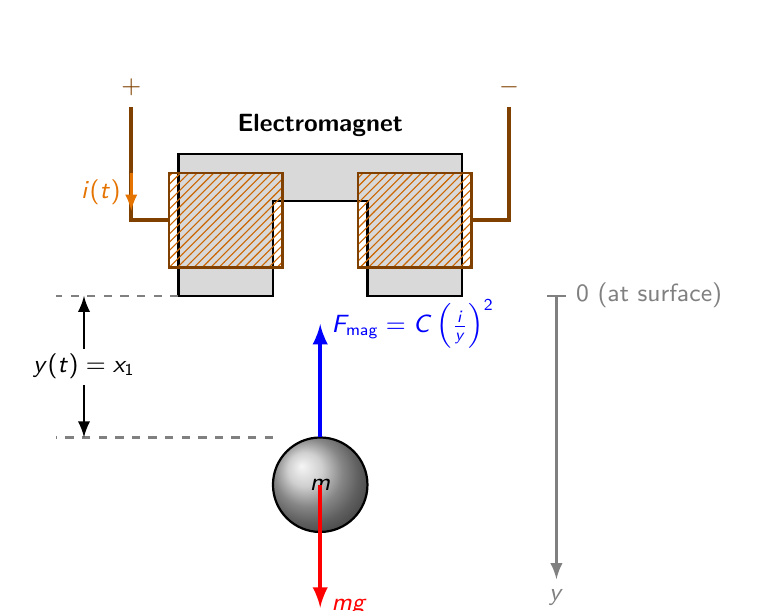
\begin{tikzpicture}[>=latex, thick, scale=1.2, font=\small\sffamily]
			
			% 1. THE ELECTROMAGNET (Stator)
			\fill[fill=gray!30, draw=black] (-1.5, 0) -- (1.5, 0) -- (1.5, -1.5) -- (0.5, -1.5) -- (0.5, -0.5) -- (-0.5, -0.5) -- (-0.5, -1.5) -- (-1.5, -1.5) -- cycle;
			
			% Coils
			\fill[pattern=north east lines, pattern color=orange!80!black, draw=orange!50!black] (-1.6, -1.2) rectangle (-0.4, -0.2);
			\fill[pattern=north east lines, pattern color=orange!80!black, draw=orange!50!black] (0.4, -1.2) rectangle (1.6, -0.2);
			
			% Wires
			\draw[orange!50!black, line width=1.5pt] (-1.6, -0.7) -- (-2, -0.7) -- (-2, 0.5) node[above] {$+$};
			\draw[orange!50!black, line width=1.5pt] (1.6, -0.7) -- (2, -0.7) -- (2, 0.5) node[above] {$-$};
			\draw[->, orange!90!black, line width=1pt] (-2, -0.2) -- (-2, -0.6) node[midway, left] {$i(t)$};
			
			\node at (0, 0.3) {\textbf{Electromagnet}};
			
			% 2. THE BALL
			% Magnet face is at y = -1.5
			% Let's place ball center at y = -3.5 (so top is at -3.0)
			\shade[ball color=gray!50] (0, -3.5) circle (0.5cm);
			\draw (0, -3.5) circle (0.5cm);
			\node at (0, -3.5) {$m$};
			
			% 3. FORCES
			\draw[->, red, line width=1.5pt] (0, -3.5) -- (0, -4.8) node[right] {$mg$};
			\draw[->, blue, line width=1.5pt] (0, -3.0) -- (0, -1.8) node[right] {$F_{\text{mag}} = C \left(\frac{i}{y}\right)^2$};
			
			
			% Reference line for Magnet Face (y=0)
			\draw[dashed, gray] (-1.5, -1.5) -- (-2.8, -1.5);
			% Reference line for Ball Top (y=y(t))
			\draw[dashed, gray] (-0.5, -3.0) -- (-2.8, -3.0);
			
			% The Gap y(t)
			\draw[<->, black, line width=1pt] (-2.5, -1.5) -- (-2.5, -3.0) node[midway, fill=white, inner sep=2pt] {$y(t) = x_1$};
			
			% Start at Magnet Face (-1.5) and point down
			\draw[->, gray, line width=1pt] (2.5, -1.5) -- (2.5, -4.5) node[below] {$y$};
			
			% Zero Mark at Magnet Face
			\draw[gray, thick] (2.4, -1.5) -- (2.6, -1.5) node[right] {$0$ (at surface)};
			
		\end{tikzpicture}
		\captionof{figure}{Schematic of the Magnetic Levitation system. The coordinate $y(t)$ is defined as the gap between the magnet face and the ball. Gravity acts in the positive $y$ direction (downwards), while the magnetic force acts in the negative direction (upwards).}
		\label{fig:maglev_schematic}
		\end{center}
	
		
		\begin{center}
		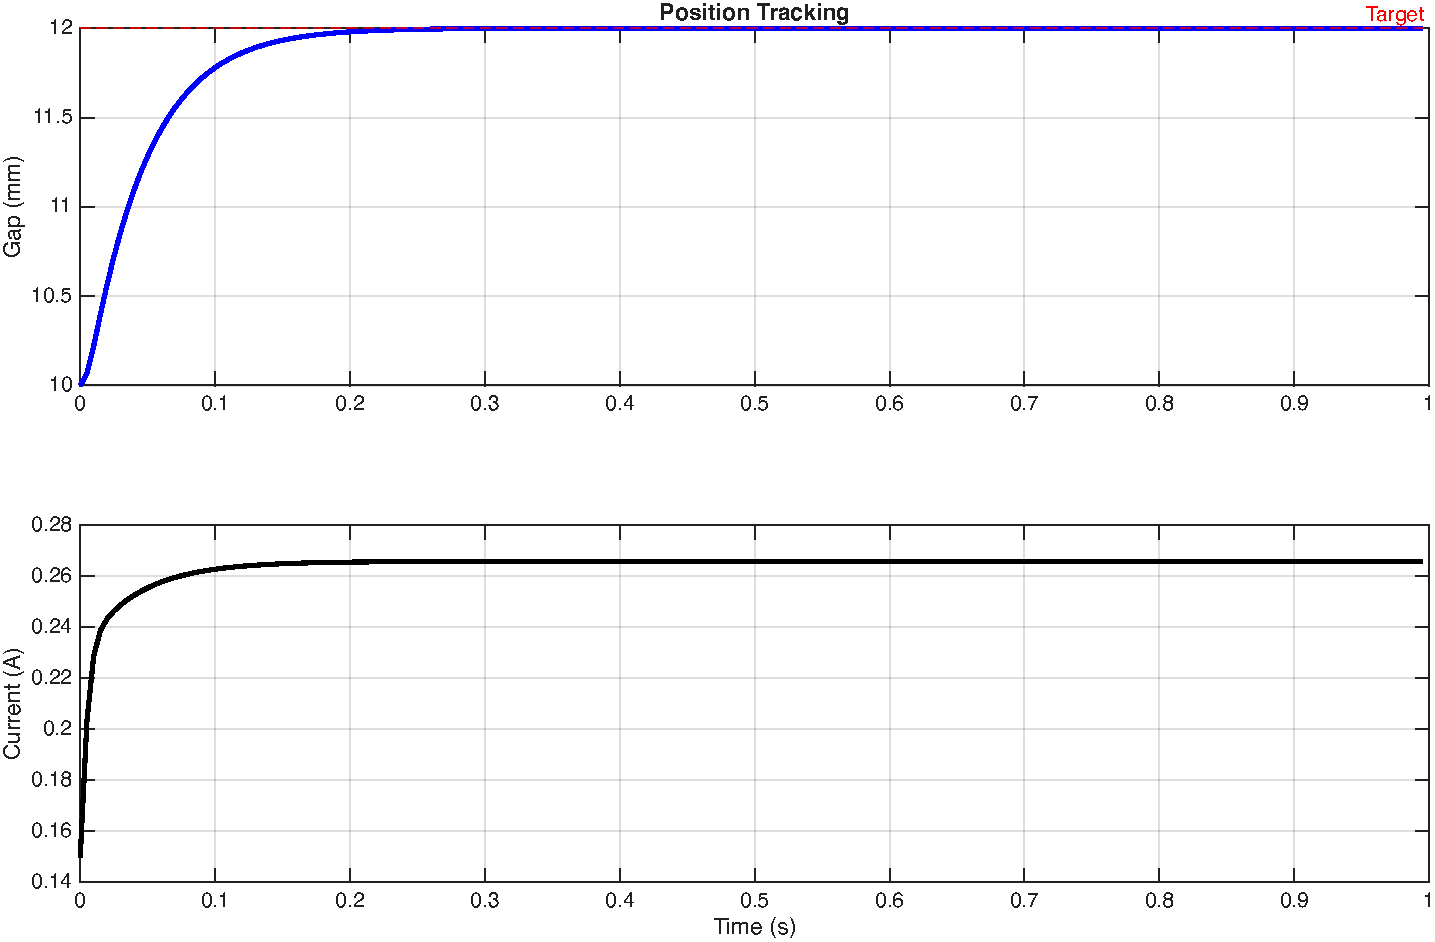
\includegraphics[width=0.7\linewidth]{Figures/Maglev.pdf}
		\captionof{figure}{Simulation results for the Magnetic Levitation setpoint tracking problem. 
			\textbf{Top:} The vertical gap (blue solid line) transitions smoothly from the initial equilibrium of 10 mm to the new target setpoint of 12 mm (red dashed line) with no overshoot. 
			\textbf{Bottom:} The control current settles at a new non-zero steady-state value ($\approx 0.26$ A). This illustrates the necessity of the feedforward term $u_g$: the current must remain non-zero to generate sufficient magnetic force to balance the weight of the ball at the new distance.}
		\label{fig:maglev}
	\end{center}
	
	
	
\end{examplebox}



\section{Chapter Summary}

This chapter has established the theoretical and numerical foundations of Optimal Control, marking the transition from system analysis to control synthesis. We introduced the LQR  as a specific instance of a broader optimisation framework.

By re-framing the classical recursive control problem as a batch QP, we laid the necessary groundwork for MPC. The key concepts covered in this chapter include:

\begin{itemize}
	\item \textbf{LQR as an Optimisation Problem:} We formulated the regulator problem as the minimisation of a quadratic cost function (penalising state deviations and control effort) subject to linear equality constraints imposed by the system dynamics.
	
	\item \textbf{The Batch Formulation:} We demonstrated how to stack decision variables into large, sparse vectors to cast the dynamic control problem into a standard static QP format ($\min \zeta^\top H \zeta$ s.t. $\mathcal{C}\zeta=d$). This perspective is critical for modern numerical solvers.
	
	\item \textbf{Equivalence of KKT and Riccati:} We proved that solving the KKT system of this QP via block back-substitution yields the classical Riccati recursion. This derivation confirmed that the optimal control law is a linear state feedback, $u_k = -K_k x_k$.
	
	\item \textbf{Infinite-Horizon Stability:} We showed that as the prediction horizon extends to infinity, the time-varying feedback gains converge to a constant steady-state value. This value can be computed directly via the Discrete Algebraic Riccati Equation (DARE), providing a static control law with guaranteed closed-loop stability.
	
	\item \textbf{Setpoint Tracking:} We extended the LQR framework from simple regulation (driving states to zero) to tracking non-zero setpoints. This requires an \textit{affine} control law combining a feedforward term (to maintain equilibrium) and a feedback term (to correct errors).
\end{itemize}

\section*{Exercises}
\begin{enumerate}
	\item Consider the discrete-time LTI system with
	\[
	A = \begin{bmatrix} 1 & 0.1 \\ 0 & 1 \end{bmatrix}, \quad B = \begin{bmatrix} 0.005 \\ 0.1 \end{bmatrix},
	\]
	and weighting matrices $Q = I_2$, $R = 1$.
	\begin{enumerate}
		\item Using the Riccati recursion with terminal cost $P_N = Q$, compute the feedback gain $K_{N-1}$ and the cost-to-go matrix $P_{N-1}$ by hand for a single backward step.
		\item Write down the resulting optimal control law $u_{N-1} = -K_{N-1}\,x_{N-1}$ and verify that the matrix $(R + B^\top P_N B)$ is invertible.
	\end{enumerate}

	\item For the same system as in Exercise~1, investigate the influence of the weighting matrices on the closed-loop behaviour.
	\begin{enumerate}
		\item Solve the DARE (using MATLAB's \texttt{dare} or an equivalent tool) for the following three design choices:
		\begin{itemize}
			\item $Q = I_2$, $R = 0.01$ \quad (cheap control),
			\item $Q = I_2$, $R = 1$ \quad (baseline),
			\item $Q = I_2$, $R = 100$ \quad (expensive control).
		\end{itemize}
		\item For each case, compute the steady-state gain $K$ and the eigenvalues of the closed-loop matrix $A_{cl} = A - BK$. Comment on how the magnitude of these eigenvalues changes as $R$ increases.
		\item Repeat the analysis by fixing $R = 1$ and varying $Q = \alpha I_2$ for $\alpha \in \{0.1,\; 1,\; 100\}$. Discuss the trade-off between fast state convergence and control effort.
	\end{enumerate}

	\item Consider the finite-horizon LQR cost function
	\[
	J = \frac{1}{2}\,x_N^\top P_N\,x_N + \sum_{k=0}^{N-1}\left(\frac{1}{2}\,x_k^\top Q\,x_k + \frac{1}{2}\,u_k^\top R\,u_k\right).
	\]
	Define the \emph{cost-to-go} at time step $k$ as
	\[
	J_k^*(x_k) = \frac{1}{2}\,x_k^\top P_k\,x_k.
	\]
	\begin{enumerate}
		\item Starting from the terminal condition $P_N = Q_N$, show by induction that $J_k^*(x_k) = \frac{1}{2}\,x_k^\top P_k\,x_k$ where $P_k$ satisfies the Riccati recursion
		\[
		P_k = Q + A^\top P_{k+1}(A - BK_k), \quad K_k = (R + B^\top P_{k+1} B)^{-1} B^\top P_{k+1} A.
		\]
		\item Explain why $P_k \succeq 0$ for all $k$ if $Q \succeq 0$, $R \succ 0$, and $P_N \succeq 0$.
	\end{enumerate}

	\item Let $P$ be the positive semi-definite solution of the DARE
	\[
	P = Q + A^\top P A - A^\top P B\,(R + B^\top P B)^{-1}\,B^\top P A.
	\]
	\begin{enumerate}
		\item Verify numerically (for the system in Exercise~1 with $Q = I_2$, $R = 1$) that $P$ is symmetric and positive definite.
		\item Substitute the computed $P$ back into the right-hand side of the DARE and confirm that both sides are equal (up to numerical precision).
		\item Define $K = (R + B^\top P B)^{-1} B^\top P A$ and compute the eigenvalues of $A_{cl} = A - BK$. Verify that all eigenvalues satisfy $|\lambda_i| < 1$, confirming closed-loop stability.
	\end{enumerate}

	\item Consider the open-loop unstable system
	\[
	A = \begin{bmatrix} 1.2 & 1 \\ 0 & 0.8 \end{bmatrix}, \quad B = \begin{bmatrix} 0 \\ 1 \end{bmatrix}.
	\]
	\begin{enumerate}
		\item Using classical pole placement, design a state-feedback gain $K_{\mathrm{pp}}$ that places the closed-loop eigenvalues of $(A - BK_{\mathrm{pp}})$ at $\lambda_1 = 0.3$ and $\lambda_2 = 0.5$.
		\item Design an infinite-horizon LQR controller for the same system with $Q = I_2$ and $R = 1$. Report the resulting gain $K_{\mathrm{lqr}}$ and the closed-loop eigenvalues.
		\item Compare the two designs: Which produces a larger control effort for the initial condition $x_0 = [1;\;0]$? Simulate both closed-loop systems for 30 time steps and discuss the differences in transient response and control magnitude. What advantages does the LQR design offer over ad-hoc pole placement?
	\end{enumerate}

	\item A student proposes to use the weighting matrices
	\[
	Q = \begin{bmatrix} 1 & 0 \\ 0 & -1 \end{bmatrix}, \quad R = 0.5
	\]
	in an LQR design.
	\begin{enumerate}
		\item Explain why this choice of $Q$ violates the convexity conditions required for a well-posed LQR problem.
		\item Provide a concrete example showing that the cost function $J = \sum_{k=0}^{N-1} \left(\frac{1}{2}\,x_k^\top Q\,x_k + \frac{1}{2}\,u_k^\top R\,u_k\right)$ can be made arbitrarily negative with this $Q$, and hence no finite minimum exists.
		\item Suggest a corrected $Q$ matrix that penalises only the first state variable (position) while leaving the second (velocity) unpenalised, and verify that it is positive semi-definite.
	\end{enumerate}
\end{enumerate}

	\chapter{State Estimation and the Kalman Filter}
\label{chap:kalman}

In the previous chapter on LQR design, we assumed that the full state vector $x_k$ was available for feedback. In practice, this is rarely the case. We typically have access only to a limited set of noisy measurements $y_k$. To implement modern control strategies like LQR or MPC, we must therefore reconstruct the internal state of the system from these imperfect observations.

While the concept of \emph{Observability} tells us \textit{if} the state can be reconstructed mathematically, it does not tell us \textit{how} to do so robustly in the presence of uncertainty. This chapter derives the optimal solution to the state estimation problem: the \textbf{Kalman Filter}~\cite{Kalman1960}.

This chapter is structured as follows:
\begin{itemize}
	\item We begin with a brief review of \emph{probability and stochastic systems}, defining the mean and covariance matrices necessary to describe uncertainty.
	\item We formulate the estimation problem and derive the \emph{recursive Kalman Filter algorithm}, showing how it optimally balances the system model against sensor data.
	\item We explore the mathematical \emph{duality between estimation and control} (LQR), revealing the deep symmetry in linear systems theory.
	\item We discuss the \emph{Steady-State Kalman Filter} and its relation to the Algebraic Riccati Equation, which simplifies implementation for time-invariant systems.
	\item Finally, we provide practical guidelines for \emph{tuning} the filter—specifically, how to select the noise covariance matrices $W$ and $V$—and demonstrate the complete design process with a MATLAB case study.
\end{itemize}

\section{Background: Stochastic Systems and Probability}

In previous chapters, we assumed that our system models were perfect and our sensors provided exact measurements. In reality, engineering systems are subject to uncertainty: actuators have jitter, sensors have noise, and mathematical models are merely approximations of complex physical reality.

To deal with this, we must transition from \textit{deterministic} variables to \textit{random variables}. In this framework, we do not know the exact state $x_k$; instead, we track the \textit{probability} of the state being at a certain location. The Kalman Filter is essentially an algorithm that propagates the mean and covariance of these probability distributions over time.

Before deriving the filter, we briefly review the essential concepts of probability theory required for linear estimation. A detailed review of the probability concepts used in this chapter is provided in Appendix~\ref{app:prob}.

\subsection{Random Variables and Expectation}

In many practical control scenarios, we cannot know the state of a system with absolute certainty due to sensor noise, model mismatch, or unknown disturbances. Consequently, we model the state not as a deterministic scalar or vector, but as a \textbf{random vector} $x \in \mathbb{R}^n$. This means $x$ does not hold a single fixed value, but is described by a probability distribution function (PDF), denoted as $p(x)$.

The most fundamental statistical property of a random variable is the \textbf{Mean} (or Expected Value). Intuitively, this represents the ``centre of gravity'' of the probability distribution, or the average value one would observe if the experiment were repeated an infinite number of times. Mathematically, it is the first moment of the distribution:
\begin{equation*}
	\mu = \mathbb{E}[x] = \int_{-\infty}^{\infty} x \, p(x) \, dx
\end{equation*}
Note that for a vector $x$, this integral is applied element-wise to each component.

A crucial property of the expectation operator $\mathbb{E}[\cdot]$ is that it is \textbf{linear}. If we apply a deterministic linear transformation to a random variable—such as multiplying it by a constant matrix $A$ or shifting it by a constant vector $b$—the mean transforms in exactly the same manner:
\begin{equation*}
	\mathbb{E}[A x + b] = A \mathbb{E}[x] + b
\end{equation*}
This property is of extreme importance in linear system theory. It implies that for a linear dynamical system (e.g., $x_{k+1} = A x_k + B u_k$), the \emph{average} behaviour of the system can be predicted simply by propagating the mean state through the deterministic system matrices, separating the deterministic dynamics from the stochastic noise.
\subsection{The Covariance Matrix}
While the mean tells us where the state is \textit{likely} to be, it tells us nothing about how confident we are in that estimate. This uncertainty is quantified by the \textbf{Covariance Matrix}, typically denoted as $P$ (or $\Sigma$).

For a random vector $x$ with mean $\mu$, the covariance is defined as the expected value of the squared error:
\begin{equation*}
	P = \text{Cov}(x) = \mathbb{E}\left[ (x - \mu)(x - \mu)^\top \right]
\end{equation*}
If $x$ has dimension $n \times 1$, then $P$ is an $n \times n$ matrix with specific properties:
\begin{itemize}
	\item \textbf{Symmetric:} $P = P^\top$.
	\item \textbf{Positive Semi-Definite:} $P \succeq 0$.
	\item \textbf{Diagonal Elements ($P_{ii}$):} Represent the \textit{variance} of the $i$-th state ($\sigma_i^2$). A large value indicates high uncertainty.
	\item \textbf{Off-Diagonal Elements ($P_{ij}$):} Represent the \textit{covariance} between state $i$ and state $j$.
\end{itemize}

\subsection{The Gaussian Distribution}
In linear estimation theory, we predominantly assume that noise and states follow a \textbf{Gaussian} (or Normal) distribution (see Appendix~\ref{app:prob} for a detailed treatment of probability distributions). A Gaussian random vector is completely defined by its mean $\mu$ and covariance $P$. We write this as:
\begin{equation*}
	x \sim \mathcal{N}(\mu, P)
\end{equation*}
The Gaussian assumption is powerful because linear transformations of Gaussian variables remain Gaussian. This property allows the Kalman Filter to define the state entirely using just two parameters: the estimate vector $\hat{x}$ (the mean) and the error covariance matrix $P$.

\subsection{White Noise}
In system modelling, we often represent disturbances as \textbf{White Noise}. A discrete-time stochastic process $w_k$ is called white noise if it is uncorrelated in time:
\begin{equation*}
	\begin{aligned}
		\mathbb{E}[w_k] &= 0 \\
		\mathbb{E}[w_k w_j^\top] &= \begin{cases} W_k & \text{if } k = j \\ 0 & \text{if } k \neq j \end{cases}
	\end{aligned}
\end{equation*}
Here, $W_k$ is the \textbf{Process Noise Covariance}. Similarly, for sensors, we define measurement noise $v_k$ with \textbf{Measurement Noise Covariance} $V_k$.

\begin{summarybox}{Key Property: Linear Propagation of Uncertainty}
	The foundation of the Kalman Filter \emph{Predict} step relies on how Gaussian distributions transform through linear systems.
	
	Consider a random state vector $x$ with mean $\hat{x}$ and covariance $P$. If this state evolves through linear dynamics with additive \emph{zero-mean} noise $w$ (where $w$ has covariance $W$):
	\[ x_{new} = A x + w \]
	
	The statistics of the new state are given by:
	\begin{itemize}
		\item \textbf{New Mean:} 
		\[ \mathbb{E}[x_{new}] = A\hat{x} \]
		\item \textbf{New Covariance:} 
		\[ \text{Cov}(x_{new}) = A P A^\top + W \]
	\end{itemize}
	
	The term $A P A^\top$ represents how the system dynamics stretch and rotate the uncertainty ellipse, while $W$ represents the additional uncertainty injected by the process noise.
\end{summarybox}

\section{Problem Formulation}

We consider the problem of estimating the internal state of a discrete-time linear system subject to stochastic disturbances. Unlike deterministic control, where the state is assumed known, here we must infer it from noisy data.

\subsection{The Stochastic System Model}
The evolution of the system and the observation process are governed by the following linear difference equations:
\begin{align*}
	x_{k+1} &= A x_k + B u_k + w_k \\
	y_k &= C x_k + v_k
\end{align*}
Here, $x_k \in \mathbb{R}^n$ is the state vector, $u_k \in \mathbb{R}^m$ is the known control input, and $y_k \in \mathbb{R}^p$ is the measured output.

\subsection{Statistical Assumptions}
To derive the optimal filter, we must rigorously define the statistical properties of the noise and the initial conditions. We assume the following:

\begin{enumerate}
\item \textbf{Process Noise ($w_k$):} Represents model mismatches and external disturbances. It is assumed to be zero-mean, white Gaussian noise with covariance matrix $W$:
\[ w_k \sim \mathcal{N}(0, W), \quad \mathbb{E}[w_k w_j^\top] = W \delta_{kj} \]
where $\delta_{kj}$ is the Kronecker delta (1 if $k=j$, 0 otherwise). This term ensures that the noise is uncorrelated in time (i.e., the disturbance at time $k$ is independent of the disturbance at any other time $j$).
	
	\item \textbf{Measurement Noise ($v_k$):} Represents sensor inaccuracies. It is assumed to be zero-mean, white Gaussian noise with covariance matrix $V$:
	\[ v_k \sim \mathcal{N}(0, V), \quad \mathbb{E}[v_k v_j^\top] = V \delta_{kj} \]
	
	\item \textbf{Initial Condition ($x_0$):} The starting state is not a fixed unknown, but a random variable with a known mean and covariance:
	\[ x_0 \sim \mathcal{N}(\bar{x}_0, P_0) \]
	
	\item \textbf{Independence:} The process noise $w_k$, measurement noise $v_k$, and initial state $x_0$ are mutually uncorrelated.
\end{enumerate}

\subsection{The Estimation Objective}
Our goal is to construct an estimate of the state, denoted as $\hat{x}_k$, using the history of measurements available up to time $k$.

We define the \textbf{estimation error} as:
\begin{equation*}
	e_k \triangleq x_k - \hat{x}_k
\end{equation*}

The problem is to find the recursive algorithm that computes $\hat{x}_k$ such that the expected value of the squared error norm (the \textbf{Mean Squared Error}) is minimised at every time step:
\begin{equation*}
	\min_{\hat{x}_k} J_k = \mathbb{E} \left[ \| e_k \|^2 \right] = \mathbb{E} \left[ (x_k - \hat{x}_k)^\top (x_k - \hat{x}_k) \right]
\end{equation*}

An estimator that satisfies this condition is known as the \textbf{Minimum Variance Unbiased Estimator (MVUE)}. Under the Gaussian assumptions listed above, the Kalman Filter is the unique solution to this problem.


\section{Derivation of the Kalman Filter}

To derive the optimal filter, we postulate a recursive linear estimator structure that operates in two distinct phases at each time step: a \textbf{Prediction} phase (based on the system model) and a \textbf{Correction} phase (based on the new measurement).

\subsection{The Estimator Structure}

Let $\hat{x}_k^-$ denote the \textit{a priori} state estimate (the prediction before processing the measurement at time $k$), and let $\hat{x}_k$ denote the \textit{a posteriori} estimate (after incorporating the measurement).

We assume the process noise $w_k$ and measurement noise $v_k$ are zero-mean, white, mutually uncorrelated, and independent of the initial estimation error, with covariances:
\[
\mathbb{E}[w_k w_k^\top] = W, \qquad \mathbb{E}[v_k v_k^\top] = V.
\]

The observer dynamics are defined as follows:

\begin{enumerate}
	\item \textbf{Prediction (Time Update):}  
	The previous estimate is propagated forward using the deterministic system dynamics:
	\begin{equation} \label{eq:obs_predict}
		\hat{x}_k^- = A \hat{x}_{k-1} + B u_{k-1}.
	\end{equation}
	
	\item \textbf{Correction (Measurement Update):}  
	The prediction is corrected using the difference between the actual measurement and the predicted measurement. This difference is called the \textbf{Innovation} ($\tilde{y}_k$):
	\begin{equation} \label{eq:obs_correct}
		\hat{x}_k = \hat{x}_k^- + L_k \underbrace{(y_k - C \hat{x}_k^-)}_{\tilde{y}_k}.
	\end{equation}
\end{enumerate}

Here, $L_k$ is the \textbf{Kalman gain}. Our objective is to determine $L_k$ such that the mean squared estimation error is minimised.

\paragraph{Step 1: Prediction Error Statistics}

Define the \textit{a priori} estimation error
\[
e_k^- \triangleq x_k - \hat{x}_k^-.
\]
Substituting the system dynamics $x_k = A x_{k-1} + B u_{k-1} + w_{k-1}$ and the prediction equation~\eqref{eq:obs_predict} yields:
\begin{align*}
	e_k^- 
	&= A(x_{k-1} - \hat{x}_{k-1}) + w_{k-1} \nonumber \\
	&= A e_{k-1} + w_{k-1}.
\end{align*}

The \textit{a priori} error covariance is defined as $P_k^- \triangleq \mathbb{E}[e_k^- (e_k^-)^\top]$.
By substituting the error dynamics into the definition of the covariance, we obtain:
\begin{equation*}
	P_k^- = \mathbb{E}\left[ (A e_{k-1} + w_{k-1}) (A e_{k-1} + w_{k-1})^\top \right].
\end{equation*}
Expanding the quadratic term yields four components:
\begin{align*}
	P_k^- &= \mathbb{E}\left[ A e_{k-1} e_{k-1}^\top A^\top + A e_{k-1} w_{k-1}^\top + w_{k-1} e_{k-1}^\top A^\top + w_{k-1} w_{k-1}^\top \right] \nonumber \\
	&= A \underbrace{\mathbb{E}[e_{k-1} e_{k-1}^\top]}_{P_{k-1}} A^\top + A \underbrace{\mathbb{E}[e_{k-1} w_{k-1}^\top]}_{0} + \underbrace{\mathbb{E}[w_{k-1} e_{k-1}^\top]}_{0} A^\top + \underbrace{\mathbb{E}[w_{k-1} w_{k-1}^\top]}_{W}.
\end{align*}
The cross-terms $\mathbb{E}[e_{k-1} w_{k-1}^\top]$ vanish because the white process noise $w_{k-1}$ is uncorrelated with the error accumulated in previous time steps. Thus, the equation simplifies to:
\begin{equation} \label{eq:cov_predict}
	P_k^- = A P_{k-1} A^\top + W.
\end{equation}

\paragraph{Step 2: Correction Error Statistics}

The \textit{a posteriori} estimation error is defined as $e_k \triangleq x_k - \hat{x}_k$.
Substituting the correction equation~\eqref{eq:obs_correct} and the measurement model $y_k = C x_k + v_k$ gives:
\begin{align*}
	e_k 
	&= (I - L_k C)e_k^- - L_k v_k.
\end{align*}

To derive the covariance update, we substitute the expression for $e_k$ into the definition $P_k = \mathbb{E}[e_k e_k^\top ]$:
\begin{equation*}
	P_k = \mathbb{E}\left[ \left( (I - L_k C)e_k^- - L_k v_k \right) \left( (I - L_k C)e_k^- - L_k v_k \right)^\top  \right].
\end{equation*}
Distributing the transpose operator $(X - Y)^\top  = X^\top  - Y^\top $ inside the second bracket gives:
\begin{equation*}
	P_k = \mathbb{E}\left[ \left( (I - L_k C)e_k^- - L_k v_k \right) \left( (e_k^-)^\top (I - L_k C)^\top - v_k^\top  L_k^\top \right) \right].
\end{equation*}
Expanding the product yields four terms:
\begin{align*}
	P_k = \mathbb{E}\bigg[ 
	\underbrace{(I - L_k C) e_k^- (e_k^-)^\top (I - L_k C)^\top}_{\text{Term 1}} 
	- \underbrace{(I - L_k C) e_k^- v_k^\top L_k^\top}_{\text{Term 2}} 
	- \underbrace{L_k v_k (e_k^-)^\top (I - L_k C)^\top}_{\text{Term 3}} 
	+ \underbrace{L_k v_k v_k^\top L_k^\top}_{\text{Term 4}} 
	\bigg].
\end{align*}
We now analyse the expectation of each term:
\begin{itemize}
	\item \textbf{Term 1:} Since $\mathbb{E}[e_k^- (e_k^-)^\top] = P_k^-$, this becomes $(I - L_k C) P_k^- (I - L_k C)^\top$.
	\item \textbf{Terms 2 \& 3:} The measurement noise $v_k$ is uncorrelated with the \textit{a priori} estimation error $e_k^-$ (which depends only on past history). Therefore, $\mathbb{E}[e_k^- v_k^\top] = 0$, and these cross-terms vanish.
	\item \textbf{Term 4:} Since $\mathbb{E}[v_k v_k^\top] = V$, this becomes $L_k V L_k^\top$.
\end{itemize}
Combining these results yields the \textbf{Joseph form} covariance update:
\begin{equation} \label{eq:cov_update_long}
	P_k = (I - L_k C) P_k^- (I - L_k C)^\top + L_k V L_k^\top.
\end{equation}

\textbf{Step 3: Optimisation of the Gain}

To derive the optimal gain, we define a cost function $J$ based on the total mean squared error of the states. This is equivalent to minimising the trace (sum of diagonal elements) of the \textit{a posteriori} covariance matrix:
\begin{equation*}
	J(L_k) = \mathrm{Tr}(P_k)
\end{equation*}

\paragraph{a) Expanding the Covariance Matrix:}
First, we substitute the full expression for $P_k$ from Eq.~\eqref{eq:cov_update_long} and expand the terms:
\begin{align*}
	P_k &= (P_k^- - L_k C P_k^-)(I - C^\top  L_k^\top) + L_k V L_k^\top \nonumber \\
	P_k &= P_k^- - P_k^- C^\top L_k^\top - L_k C P_k^- + L_k C P_k^- C^\top L_k^\top+ L_k V L_k^\top
\end{align*}
We can group the quadratic terms involving $L_k$:
\begin{equation} \label{eq:Pk_expanded}
	P_k = P_k^- - P_k^- C^\top L_k^\top - L_k C P_k^- + L_k (C P_k^- C^\top + V) L_k^\top
\end{equation}

\paragraph{b) Matrix Calculus Rules:}
To minimise $J$ with respect to the matrix $L_k$, we use the following standard matrix derivative identities:
\begin{itemize}
	\item $\frac{\partial}{\partial X} \mathrm{Tr}(X A) = A^\top $
	\item $\frac{\partial}{\partial X} \mathrm{Tr}(A X^\top ) = A$
	\item $\frac{\partial}{\partial X} \mathrm{Tr}(X A X^\top) = 2 X A$ (if $A$ is symmetric)
\end{itemize}
Note that the trace is invariant under transpose, so $\mathrm{Tr}(P_k^- C^\top  L_k^\top) = \mathrm{Tr}((P_k^- C^\top L_k^\top)^\top) = \mathrm{Tr}(L_k C P_k^-)$. Thus, the two linear terms in \eqref{eq:Pk_expanded} contribute identically to the derivative.

\paragraph{c) Taking the Derivative:}
We differentiate $J = \mathrm{Tr}(P_k)$ with respect to $L_k$ and set the result to zero:
\begin{equation*}
	\frac{\partial J}{\partial L_k} = \underbrace{0}_{\text{Const}} - \underbrace{2 P_k^- C^\top}_{\text{Linear Terms}} + \underbrace{2 L_k (C P_k^- C^\top + V)}_{\text{Quadratic Terms}} = 0
\end{equation*}

\paragraph{d) Solving for the Optimal Gain:}
Rearranging the equation yields:
\begin{equation*}
	L_k (C P_k^- C^\top + V) = P_k^- C^\top
\end{equation*}
The term in the parentheses represents the uncertainty of the measurement prediction. We define this as the \textbf{Innovation Covariance}, $S_k$:
\begin{equation*}
	S_k \triangleq C P_k^- C^\top + V
\end{equation*}
Multiplying from the right by $S_k^{-1}$ gives the explicit solution for the optimal Kalman gain:
\begin{equation} \label{eq:opt_gain}
	\boxed{ L_k = P_k^- C^\top S_k^{-1} }
\end{equation}

\paragraph{e) Simplifying the Covariance Update:}
The full update equation \eqref{eq:Pk_expanded} is computationally expensive. We can simplify it by substituting the optimality condition back into the equation.
From \eqref{eq:opt_gain}, we know that $L_k S_k = P_k^- C^\top $.
Substituting this into the quadratic term of Eq.~\eqref{eq:Pk_expanded}:
\begin{align*}
	L_k \underbrace{(C P_k^- C^\top  + V)}_{S_k} L_k^\top  &= (L_k S_k) L_k^\top  \nonumber \\
	&= (P_k^- C^\top ) L_k^\top 
\end{align*}
We substitute this back into the expanded covariance equation:
\begin{align*}
	P_k &= P_k^- \cancel{- P_k^- C^\top  L_k^\top } - L_k C P_k^- + \cancel{P_k^- C^\top  L_k^\top } \nonumber \\
	 &= P_k^- - L_k C P_k^-
\end{align*}
Factoring out $P_k^-$ from the right yields the canonical covariance update equation:
\begin{equation*}
	\boxed{ P_k = (I - L_k C) P_k^- }
\end{equation*}
\textit{Note:} While this simple form is mathematically correct for the optimal gain, numerical implementations often use the longer \emph{Joseph form} (Eq. \ref{eq:cov_update_long}) because it guarantees the resulting matrix remains symmetric and positive definite even in the presence of floating-point rounding errors.

\begin{summarybox}{The Discrete-Time Kalman Filter Algorithm}
	\textbf{Predict:}
	\begin{align*}
		\hat{x}_k^- &= A \hat{x}_{k-1} + B u_{k-1} \\
		P_k^- &= A P_{k-1} A^\top  + W
	\end{align*}
	
	\textbf{Compute Gain:}
	\begin{align*}
		S_k &= C P_k^- C^\top  + V \\
		L_k &= P_k^- C^\top  S_k^{-1}
	\end{align*}
	
	\textbf{Correct:}
	\begin{align*}
		\hat{x}_k &= \hat{x}_k^- + L_k (y_k - C \hat{x}_k^-) \\
		P_k &= (I - L_k C) P_k^-
	\end{align*}
\end{summarybox}


\section{The Steady-State Kalman Filter}

In the recursive derivation above, the estimation error covariance $P_k$ and the Kalman gain $L_k$ are re-calculated at every time step. This is computationally expensive.

However, for \textbf{Linear Time-Invariant (LTI)} systems—where $A, B, C, W, V$ are constant—the covariance matrix $P_k^-$ converges to a constant steady-state matrix $P_{\infty}$ as $k \to \infty$, provided certain structural properties are met.

\subsection{Convergence Conditions}
\label{sec:kalman_convergence}
Convergence is guaranteed if the system satisfies two conditions related to observability and controllability:
\begin{enumerate}
	\item The pair $(A, C)$ must be \textbf{Detectable}. This ensures that any unstable mode in the system is visible at the output $y$, allowing the filter to correct it.
	\item The pair $(A, W^{1/2})$ must be \textbf{Stabilisable}. Here, $W^{1/2}$ is the matrix square root of the process noise covariance ($W = W^{1/2}(W^{1/2})^\top$). Intuitively, this condition requires that the process noise "excites" all unstable modes of the system. If an unstable mode is not excited by noise and cannot be seen by sensors, its estimation error variance will grow unbounded.
\end{enumerate}

\subsection{The Discrete Algebraic Riccati Equation (DARE)}
When these conditions are met, the \textit{a priori} covariance $P_{\infty}$ satisfies the \textbf{Discrete Algebraic Riccati Equation}:
\begin{equation*}
	P_\infty = A P_\infty A^\top + W 
	- A P_\infty C^\top (C P_\infty C^\top + V)^{-1} C P_\infty A^\top.
\end{equation*}
Consequently, the Kalman gain also converges to a constant matrix:
\begin{equation*}
	L_\infty = P_\infty C^\top (C P_\infty C^\top + V)^{-1}.
\end{equation*}

\subsection{The Constant Gain Implementation}
Using the steady-state gain $L_\infty$ simplifies the algorithm significantly. We no longer need to update covariance matrices online. The filter reduces to a standard linear state-space system.

We can implement this in two ways:

\paragraph{1. The Two-Step Form (Standard):}
This preserves the predict-correct structure but uses a fixed gain.
\begin{align*}
	\textbf{Correct:} \quad \hat{x}_k &= \hat{x}_k^- + L_\infty (y_k - C \hat{x}_k^-) \\
	\textbf{Predict:} \quad \hat{x}_{k+1}^- &= A \hat{x}_k + B u_k
\end{align*}

\paragraph{2. The One-Step Form (Luenberger):}
We can substitute the correction step into the prediction step to create a single update equation:
\begin{equation*}
	\hat{x}_{k+1}^- = A \hat{x}_k^- + B u_k + \underbrace{A L_\infty}_{L_{pred}} (y_k - C \hat{x}_k^-)
\end{equation*}
\begin{notebox}{Implementation Warning}
	Note the term $A L_\infty$ in the one-step form. This is because standard Kalman gains correct the \textit{current} estimate, while the one-step form updates the \textit{prediction} for the next step directly. When implementing this on a microcontroller, ensure you apply the gain at the correct point in the loop.
\end{notebox}

\section{Duality between Estimation and Control}

A remarkable result in linear systems theory is the mathematical symmetry, or \textbf{duality}, between the optimal control problem (LQR) and the optimal estimation problem (Kalman Filter).

In the LQR problem, we propagate a cost matrix $P$ \textit{backwards} in time (from the future horizon to the present) to minimise a weighted sum of states and inputs. In the Kalman Filter, we propagate an error covariance matrix $P$ \textit{forwards} in time (from the initial condition to the present) to minimise the mean squared estimation error.

Despite the difference in the direction of time, the recursive equations governing these two matrices are identical under a specific substitution of variables. This means that the \textbf{same numerical algorithms} (such as the Riccati solver) used to design a controller can be used to design an observer.

\begin{table}[h]
	\centering
	\caption{The Duality Mappings. To solve for the Kalman Gain using an LQR solver, substitute the LQR parameters (left) with the corresponding KF parameters (right).}
	\label{tab:duality}
	\renewcommand{\arraystretch}{1.3} % More vertical space
	\begin{tabular}{lcc}
		\toprule
		\textbf{Property} & \textbf{LQR (Control)} & \textbf{Kalman Filter (Estimation)} \\
		\midrule
		\textbf{Direction} & Backward ($t \leftarrow T$) & Forward ($0 \to t$) \\
		\textbf{Dynamics} & $A$ & $A^\top$ \\
		\textbf{Actuation/Sensing} & $B$ & $C^\top$ \\
		\textbf{State Penalty / Noise} & $Q$ & $W$ (Process Noise) \\
		\textbf{Input Penalty / Noise} & $R$ & $V$ (Measurement Noise) \\
		\textbf{Resulting Gain} & $K$ (Feedback) & $L^\top$ (Observer) \\
		\bottomrule
	\end{tabular}
\end{table}

\subsection{Implications for Implementation}
This duality allows us to compute the steady-state Kalman gain $L_{\infty}$ using standard LQR commands in software like MATLAB. 

Recall that the MATLAB command for LQR is:
\begin{lstlisting}
	[K, P, E] = dlqr(A, B, Q, R);
\end{lstlisting}

By applying the substitutions from Table \ref{tab:duality}, we can compute the optimal estimator gain using the \texttt{dare} solver to obtain the steady-state error covariance $P_\infty$, and then form the gain directly:
\begin{lstlisting}
	% Solve the dual DARE for the steady-state error covariance
	[P_inf, ~, ~] = dare(A', C', W, V);

	% Compute the steady-state Kalman gain: L = P*C'*(C*P*C'+V)^{-1}
	L = P_inf * C' / (C * P_inf * C' + V);
\end{lstlisting}
This indicates that if the pair $(A, C)$ is detectable and $(A, W^{1/2})$ is stabilisable (see Section~\ref{sec:kalman_convergence}), the Kalman filter estimates will converge, just as an LQR controller stabilises a controllable system. Observability and controllability are sufficient but stronger conditions.


\section{Practical Tuning: Selecting $W$ and $V$}

While the system matrices ($A, B, C$) obey physical laws, the noise covariance matrices often serve as tuning parameters that dictate the filter's \textbf{behaviour}.

\subsection{Measurement Noise ($V$)}
This matrix represents sensor precision and is straightforward to determine. It is typically diagonal (assuming uncorrelated sensors) and obtained via:
\begin{itemize}
	\item \textbf{Datasheets:} Using the manufacturer's specified noise variance ($\sigma^2$).
	\item \textbf{Experimentation:} Logging data from a stationary sensor and computing the statistical variance of the signal.
\end{itemize}

\subsection{Process Noise ($W$) }
The matrix $W$ is more abstract. It lumps together physical disturbances (e.g., wind gusts) and \textbf{modelling errors} (e.g., linearisation inaccuracies). Since these are difficult to quantify, $W$ is treated as a tuning handle to adjust the trade-off between the model and the measurements:

\begin{itemize}
	\item \textbf{High $W$ (Trust the Sensor):} The filter assumes the model is poor. The Kalman gain $L$ increases. Result: Fast transient response, but the estimate will be noisy.
	\item \textbf{Low $W$ (Trust the Model):} The filter assumes the model is accurate. The Kalman gain $L$ decreases. Result: Smooth estimates (noise rejection), but the filter will lag during sudden changes.
\end{itemize}

\textbf{Practical Rule:} Fix $V$ based on physical sensor data, then tune $W$ until the desired balance between smoothness and responsiveness is achieved.

\begin{examplebox}{MATLAB: Kalman Filter Implementation (LQG Control)}
	\textbf{The Problem:}
	Consider the double integrator system (representing a simple mass). Our objective is to stabilise the system using full-state feedback ($u_k = -K x_k$). However, we face a practical constraint: we can only measure the \textbf{position}, and that measurement is corrupted by noise. We cannot measure the velocity directly.
	
	\textbf{The Solution:}
	We design a \textbf{Linear Quadratic Gaussian (LQG)} controller. This consists of two parts:
	\begin{enumerate}
		\item An \textbf{LQR Controller} ($K$) designed for the ideal system to regulate state to zero.
		\item A \textbf{Steady-State Kalman Filter} ($L$) to reconstruct the velocity from the noisy position data.
	\end{enumerate}
	
	\textbf{The Code:}
	The script below computes the optimal gains using the duality principle ($A \to A^\top$, $B \to C^\top$) and simulates the closed-loop system.
	
	\begin{lstlisting}[language=Matlab, caption={Closed-loop simulation of LQR control using Kalman Filter estimates.}, label=lst:kalman_code]
		clear; clc; close all;
		
		dt = 0.1;
		A = [1, dt; 0, 1];     		% States: [Position; Velocity]
		B = [0.5*dt^2; dt];    	% Input: Force
		C = [1, 0];            			% Output: Position only
		
		Q_lqr = eye(2);        
		R_lqr = 0.1;           
		
		% B. Estimator Covariances (Kalman Filter)
		% W: Process Noise Covariance (Trust in Model)
		% V: Measurement Noise Covariance (Trust in Sensor)
		W = 1e-4 * eye(2);     
		V = 1e-2;          
		
		%% Compute Gains (Offline)
		% A. Controller Gain (K)
		[K, ~, ~] = dlqr(A, B, Q_lqr, R_lqr);
		
		% B. Estimator Gain (L)
		% Solve the dual DARE for the steady-state error covariance P_ss
		[P_ss, ~, ~] = dare(A', C', W, V);

		% Compute steady-state Kalman gain: L = P*C'*(C*P*C'+V)^{-1}
		L = P_ss * C' / (C * P_ss * C' + V);
		
		% Calculate theoretical 3-sigma error bounds for plotting
		sigma_pos = sqrt(P_ss(1,1));
		sigma_vel = sqrt(P_ss(2,2));
		
		%% Simulation Setup
		T_final = 10;
		N = floor(T_final/dt);
		t_vec = 0:dt:T_final-dt;
		
		x_true = [0.5; -0.5];   % Physical truth (starts with error)
		x_est  = [0; 0];        % Estimator initial guess (starts at 0)
		
		log_x_true = zeros(2, N);
		log_x_est  = zeros(2, N);
		log_y_meas = zeros(1, N);
		

		for k = 1:N

				w_k = sqrt(1e-4) * randn(2,1); % Process noise
				v_k = sqrt(1e-2) * randn;      % Measurement noise
		
				y_k = C * x_true + v_k;
		
				y_tilde = y_k - C * x_est;
				x_est = x_est + L * y_tilde;
		
				u_k = -K * x_est;
		
				x_est_next = A * x_est + B * u_k;
				x_true_next = A * x_true + B * u_k + w_k;
		
				log_x_true(:,k) = x_true;
				log_x_est(:,k)  = x_est;
				log_y_meas(k)   = y_k;
		
				x_true = x_true_next;
				x_est  = x_est_next;
		end
	\end{lstlisting}
	
	\textbf{Result:}
	Simulation results (Figure \ref{fig:kalman_results}) confirm the filter's performance. Even though the velocity is never measured directly, the Kalman Filter converges to the true velocity within a few seconds, allowing the LQR controller to stabilise the system effectively.
\end{examplebox}
\begin{figure}[h]
	\centering
	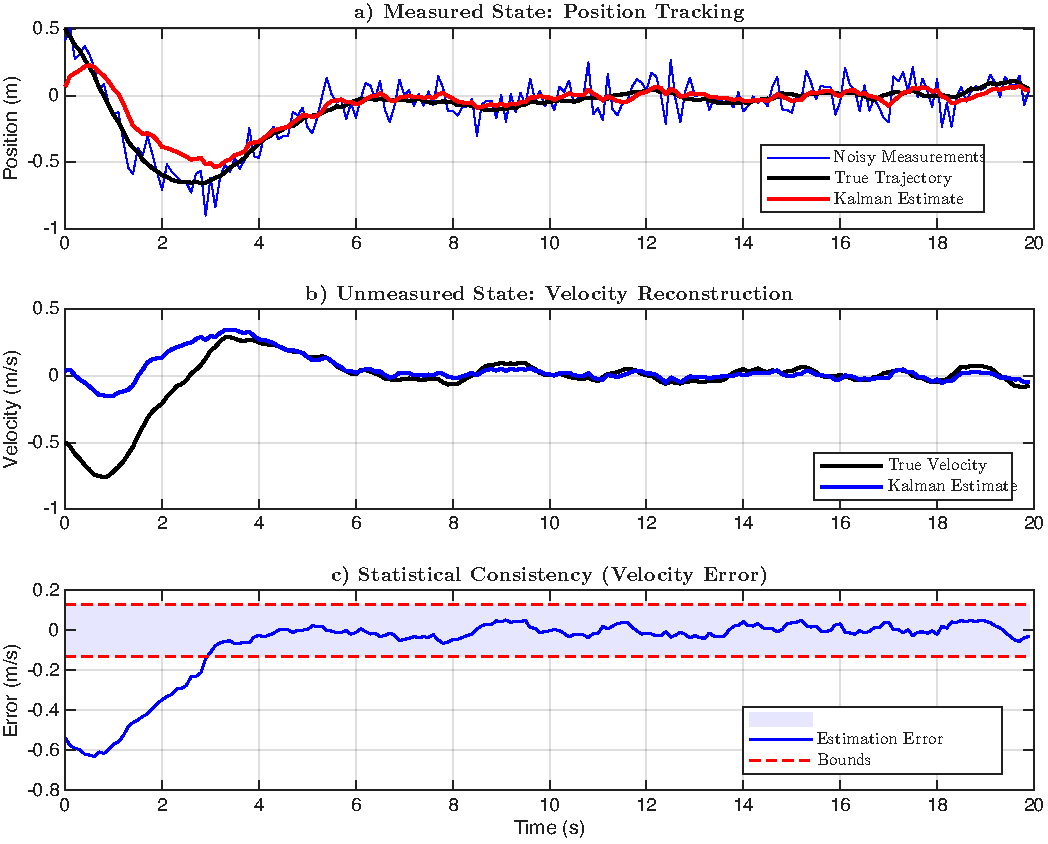
\includegraphics[width=0.9\linewidth]{Figures/Kalman_Performance}
	\caption{Simulation results for the LQG control example. 
	\textbf{(a)} Measured State: The Kalman Filter estimate (red) effectively filters the noisy position measurements (blue) to track the true trajectory (black).
	\textbf{(b)} Unmeasured State: Although velocity is not measured directly, the filter successfully reconstructs it using the system model and position data. Note the convergence of the estimate (blue) to the truth (black) after the initial transient.
	\textbf{(c)} Statistical Consistency: The velocity estimation error (blue) remains bounded within the $\pm 3\sigma$ confidence intervals (red dashed lines) derived from the steady-state covariance $P_\infty$. The large error at $t < 4$s is due to the incorrect initial guess ($x_{est}=0$ vs $x_{true}=0.5$), which the filter quickly corrects.}
	\label{fig:kalman_results}
\end{figure}

\section*{Exercises}

\begin{enumerate}

\item \textbf{Scalar Kalman Filter by Hand.}
Consider a scalar system with $A = 1$, $B = 0$, $C = 1$, process noise covariance $W = 0.5$, and measurement noise covariance $V = 2$. The initial conditions are $\hat{x}_0 = 0$ and $P_0 = 1$.

You receive the following measurements: $y_1 = 1.2$, $y_2 = 0.9$, $y_3 = 1.5$.

For each time step $k = 1, 2, 3$, carry out the full Kalman filter recursion by hand:
\begin{enumerate}
	\item Compute the predicted estimate $\hat{x}_k^-$ and predicted error variance $P_k^-$.
	\item Compute the innovation covariance $S_k = C P_{k}^{-} C^\top + V$ and the Kalman gain $L_k = P_{k}^{-} C^\top S_k^{-1}$.
	\item Compute the corrected estimate $\hat{x}_k = \hat{x}_k^- + L_k(y_k - C\hat{x}_k^-)$ and the updated error variance $P_k = (1 - L_k C) P_k^-$.
\end{enumerate}
Comment on how the Kalman gain and error variance evolve over the three steps.

\item \textbf{Effect of $W$ and $V$ on the Kalman Gain.}
Consider the same scalar system as in Exercise~1 ($A = 1$, $C = 1$), but now treat the noise covariances as parameters.

\begin{enumerate}
	\item For the steady-state case, show that the scalar Kalman gain satisfies
	\[
		L_\infty = \frac{P_\infty}{P_\infty + V},
	\]
	where $P_\infty$ is the steady-state predicted error variance.
	\item Analyse the two limiting cases:
	\begin{itemize}
		\item $W \gg V$ (process noise dominates): What happens to $L_\infty$? What does this mean physically?
		\item $W \ll V$ (measurement noise dominates): What happens to $L_\infty$? What does this mean physically?
	\end{itemize}
	\item Fix $V = 1$ and compute the steady-state Kalman gain for $W \in \{0.01,\, 0.1,\, 1,\, 10\}$. Discuss how the filter transitions from ``trusting the model'' to ``trusting the sensor'' as $W$ increases.
\end{enumerate}

\item \textbf{Steady-State Kalman Gain via the DARE.}
Consider the double integrator system from the MATLAB example in this chapter:
\[
A = \begin{bmatrix} 1 & \Delta t \\ 0 & 1 \end{bmatrix}, \quad
B = \begin{bmatrix} \tfrac{1}{2}\Delta t^2 \\ \Delta t \end{bmatrix}, \quad
C = \begin{bmatrix} 1 & 0 \end{bmatrix},
\]
with $\Delta t = 0.1$, $W = 10^{-4} I_2$, and $V = 10^{-2}$.

\begin{enumerate}
	\item Write out the Discrete Algebraic Riccati Equation (DARE) that determines the steady-state predicted error covariance $P_\infty$.
	\item Using the duality between estimation and control (Table~\ref{tab:duality}), explain how to compute $P_\infty$ and $L_\infty$ using a standard LQR solver by substituting $A \to A^\top$, $B \to C^\top$, $Q \to W$, $R \to V$.
	\item Verify numerically (e.g.\ in MATLAB using \texttt{dare(A', C', W, V)}) that the steady-state gain $L_\infty$ is consistent with the values used in the chapter's simulation.
\end{enumerate}

\item \textbf{Augmented State Estimation: Constant Disturbance.}
Consider a scalar plant
\[
	x_{k+1} = a\, x_k + b\, u_k + d_k + w_k, \qquad y_k = c\, x_k + v_k,
\]
where $d_k$ is an unknown but \emph{constant} disturbance ($d_{k+1} = d_k$). The noise $w_k$ and $v_k$ have covariances $W$ and $V$, respectively.

\begin{enumerate}
	\item Define the augmented state vector $\bar{x}_k = \begin{bmatrix} x_k \\ d_k \end{bmatrix}$ and derive the augmented system matrices $\bar{A}$, $\bar{B}$, and $\bar{C}$ such that
	\[
		\bar{x}_{k+1} = \bar{A}\,\bar{x}_k + \bar{B}\,u_k + \bar{w}_k, \qquad y_k = \bar{C}\,\bar{x}_k + v_k.
	\]
	State the augmented process noise covariance $\bar{W}$, assuming that the disturbance drift has a small variance $W_d$.
	\item Discuss what conditions on the pair $(\bar{A}, \bar{C})$ are needed for the augmented Kalman filter to converge (i.e.\ detectability of the augmented system).
	\item For $a = 0.9$, $b = 1$, $c = 1$, $W = 0.01$, $V = 0.1$, and $W_d = 10^{-4}$, set up the DARE for the augmented system and explain how the resulting steady-state gain $\bar{L}_\infty$ simultaneously estimates $x_k$ and $d_k$.
\end{enumerate}

\item \textbf{Comparing Prediction and Update Steps.}
Consider a system with
\[
A = \begin{bmatrix} 0.8 & 0.1 \\ 0 & 0.95 \end{bmatrix}, \quad
C = \begin{bmatrix} 1 & 0 \end{bmatrix}, \quad
W = \begin{bmatrix} 0.1 & 0 \\ 0 & 0.05 \end{bmatrix}, \quad
V = 0.5.
\]
At time step $k$, suppose the corrected estimate and covariance are
\[
\hat{x}_{k-1} = \begin{bmatrix} 2.0 \\ 1.0 \end{bmatrix}, \qquad
P_{k-1} = \begin{bmatrix} 0.3 & 0.05 \\ 0.05 & 0.2 \end{bmatrix}.
\]
\begin{enumerate}
	\item Compute the predicted estimate $\hat{x}_k^- = A\hat{x}_{k-1}$ (assuming $u_{k-1} = 0$) and the predicted covariance $P_k^- = A P_{k-1} A^\top + W$.
	\item Compare $\mathrm{Tr}(P_{k-1})$ with $\mathrm{Tr}(P_k^-)$. Explain why the trace increases during prediction.
	\item Suppose the measurement at time $k$ is $y_k = 1.85$. Compute the innovation $\tilde{y}_k = y_k - C\hat{x}_k^-$, the innovation covariance $S_k$, the Kalman gain $L_k$, the corrected estimate $\hat{x}_k$, and the corrected covariance $P_k = (I - L_k C) P_k^-$.
	\item Compare $\mathrm{Tr}(P_k^-)$ with $\mathrm{Tr}(P_k)$. Explain why the trace decreases during the correction step.
\end{enumerate}

\item \textbf{Observability and Filter Convergence.}
Consider a two-state system with
\[
A = \begin{bmatrix} 1 & 1 \\ 0 & 1 \end{bmatrix}, \quad C_1 = \begin{bmatrix} 1 & 0 \end{bmatrix}, \quad C_2 = \begin{bmatrix} 0 & 0 \end{bmatrix}.
\]
\begin{enumerate}
	\item Compute the observability matrix $\mathcal{O} = \begin{bmatrix} C \\ CA \end{bmatrix}$ for both $C_1$ and $C_2$. Which system is observable?
	\item For the observable case ($C_1$), explain why the Kalman filter covariance $P_k$ is guaranteed to converge to a finite steady-state value $P_\infty$ (assuming $W > 0$).
	\item For the unobservable case ($C_2$), explain why $P_k$ grows without bound regardless of the choice of $W$ and $V$.  What does this imply about the practical feasibility of state estimation?
\end{enumerate}

\end{enumerate}


	\part{Model Predictive Control}

\chapter{Linear Model Predictive Control}
\label{chap:linear_mpc}

\begin{quote}
	\textit{``MPC is like playing chess: you predict several moves ahead, pick the best move, execute it, and then -- because the opponent [uncertainty] might play differently than expected -- you re-evaluate the board and plan again.''} \\
	\hfill --- paraphrasing the receding horizon principle
\end{quote}

This chapter extends unconstrained optimal control (LQR) to handle physical limits. We define the Linear MPC problem, showing how actuator saturation and safety constraints are incorporated directly into the optimisation. We then cover the \emph{Receding Horizon} principle, introduce the \emph{YALMIP} toolbox for implementation, and analyse how the prediction horizon $N$ and the terminal cost $P$ affect closed-loop stability and performance.

\section{Motivation: The Need for Constraints}

In the previous chapters, we derived the Linear Quadratic Regulator (LQR). This method provides a closed-form solution to the optimal control problem, yielding a static feedback gain matrix $K$. However, LQR relies on a critical, often unrealistic assumption: \emph{the system operates in an unconstrained linear world.}

In physical reality, every engineering system has limits:
\begin{itemize}
	\item \textbf{Actuator Saturation:} A motor has a maximum voltage; a valve cannot open beyond 100\%.
	\item \textbf{Safety Constraints:} A chemical reactor must not exceed a critical pressure; a robotic arm must stay within a defined workspace.
	\item \textbf{Performance Bounds:} A passenger vehicle must limit acceleration to ensure comfort.
\end{itemize}

\subsection*{Why \emph{Clipping} in LQR Fails}
A common naive approach is to design an LQR controller and simply \emph{clip} or saturate the control signal if it exceeds the limit: 
\[ u = \text{sat}(-Kx) = \begin{cases}
	u_\text{max} & -Kx \ge u_\text{max} \\
	u_\text{min} & -Kx \le u_\text{min} \\
	-Kx & \text{otherwise}
\end{cases} \]
While this works for small disturbances, it breaks the mathematical guarantee of optimality and stability. Saturating the input effectively turns a linear system into a non-linear one. If the LQR controller requests a strong braking force to stabilise a fast-moving vehicle, but the actuator saturates, the vehicle may overshoot or become unstable because the "planned" energy dissipation did not occur.

\subsection*{From Offline Gains to Online Optimisation}
\emph{Model Predictive Control (MPC)} fundamentally alters this approach. Instead of calculating a control law \textit{offline} (like the LQR gain $K$), MPC solves a constrained optimisation problem \textit{online} at every time step.

By incorporating the constraints directly into the prediction model, MPC "knows" about the limits in advance. It does not blindly request impossible inputs; instead, it plans a trajectory that rides the very edge of the feasible region without crossing it. This capability—to operate safely and optimally against constraints—is what makes MPC the standard in advanced industrial control.

In this chapter, we will formulate the Linear MPC problem and demonstrate how to implement it efficiently using the YALMIP toolbox.

\section{Problem Formulation}
\label{sec:mpc_formulation}

The fundamental goal of MPC is to compute a sequence of future control inputs that drives the system state to the origin (or a target setpoint) whilst satisfying all physical constraints.

At every sampling instant $t$, we measure the current state of the system, denoted as $x(t)$. We then define an optimal control problem over a finite \emph{prediction horizon} of $N$ steps. To distinguish the prediction from the actual system evolution, we use the index $k$ to denote the steps into the future (where $k=0$ represents the current time $t$).

We solve the following constrained optimisation problem:

\begin{equation} \label{eq:mpc_cost}
	\min_{{u}, {x}} J = \underbrace{x_N^\top Q_N x_N}_{\text{Terminal Cost}} + \sum_{k=0}^{N-1} \left( \underbrace{x_k^\top Q x_k}_{\text{State Penalty}} + \underbrace{u_k^\top R u_k}_{\text{Control Effort}} \right)
\end{equation}

\textbf{Subject to:}
\begin{align*}
	\textbf{Initialisation:} \quad & x_0 = x(t) && (\text{Current measured state}) \\
	\textbf{Model Dynamics:} \quad & x_{k+1} = A x_k + B u_k, && k=0,\dots,N-1 \\
	\textbf{Actuator Limits:} \quad & u_{\min} \le u_k \le u_{\max}, && k=0,\dots,N-1 \\
	\textbf{Safety Limits:} \quad & x_{\min} \le x_k \le x_{\max}, && k=1,\dots,N
\end{align*}

Where:
\begin{itemize}
	\item ${u} = \{u_0, u_1, \dots, u_{N-1}\}$ is the sequence of future control inputs to be optimised.
	\item ${x} = \{x_1, x_2, \dots, x_N\}$ is the sequence of predicted states.
	\item $Q \succeq 0$ and $R \succ 0$ are the stage cost weighting matrices.
	\item $Q_N \succeq 0$ is the terminal weight, often chosen to approximate the infinite-horizon cost (i.e., the solution to the Riccati equation, $P$).
\end{itemize}

\section{The Receding Horizon Principle}
The defining feature of MPC is its \emph{Receding Horizon} strategy. Rather than computing a single fixed trajectory from start to finish, the controller operates in a loop:

\begin{enumerate}
	\item \textbf{Measure:} Obtain the current state $x(t)$.
	\item \textbf{Solve:} Compute the optimal sequence $\{u_0, u_1, \dots, u_{N-1}\}$ by solving the constrained optimisation problem (\ref{eq:mpc_cost}).
	\item \textbf{Apply:} Inject \emph{only the first input} $u_0$ into the system. The rest of the sequence is discarded.
	\item \textbf{Recede:} Wait for the next sampling instant $t+1$, measure the new state $x(t+1)$, and repeat the process.
\end{enumerate}

By re-solving the problem at every time step based on fresh measurements, the MPC converts an open-loop optimal plan into a \emph{closed-loop feedback strategy}, capable of rejecting disturbances and correcting model mismatches.

\begin{examplebox}{Hand-Worked MPC: Scalar Integrator with Constraints}
We now solve the MPC problem \emph{entirely by hand} to make the mechanics concrete before moving to MATLAB.

\textbf{System:}
\[
x_{k+1} = x_k + u_k \qquad \text{(pure integrator)}
\]
\textbf{Parameters:} $Q = 1$, $R = 1$, $Q_N = 1$, prediction horizon $N = 2$, input constraint $|u_k| \le 0.5$.

\textbf{Initial condition:} $x_0 = 1$.

\textbf{Step 1 --- Write the predicted states in terms of the decisions:}
\begin{align*}
x_1 &= x_0 + u_0 = 1 + u_0 \\
x_2 &= x_1 + u_1 = 1 + u_0 + u_1
\end{align*}

\textbf{Step 2 --- Substitute into the cost function:}
\begin{align*}
J &= \underbrace{x_0^2}_{=1} + u_0^2 + \underbrace{x_1^2}_{(1+u_0)^2} + u_1^2 + \underbrace{x_2^2}_{(1+u_0+u_1)^2}
\end{align*}
Expanding and collecting:
\[
J = 3 + 4u_0 + 2u_1 + 3u_0^2 + 2u_0 u_1 + 2u_1^2
\]
This is a quadratic in $u = [u_0 \;\; u_1]^\top$:
\[
J = u^\top \underbrace{\begin{bmatrix} 3 & 1 \\ 1 & 2 \end{bmatrix}}_{H} u + \underbrace{\begin{bmatrix} 4 \\ 2 \end{bmatrix}^\top}_{f^\top} u + 3
\]

\textbf{Step 3 --- Solve the unconstrained QP:}

Setting $\nabla_{u} J = 2Hu + f = 0$:
\[
u^\star = -\tfrac{1}{2}H^{-1}f = -\frac{1}{2} \cdot \frac{1}{5}\begin{bmatrix} 2 & -1 \\ -1 & 3 \end{bmatrix}\begin{bmatrix} 4 \\ 2 \end{bmatrix} = -\frac{1}{10}\begin{bmatrix} 6 \\ 2 \end{bmatrix} = \begin{bmatrix} -0.6 \\ -0.2 \end{bmatrix}
\]

\textbf{Step 4 --- Check constraints:}

Since $|u_0^\star| = 0.6 > 0.5$, the constraint is violated. We set $u_0 = -0.5$ (at its bound) and re-optimise over $u_1$ alone:
\[
x_1 = 1 - 0.5 = 0.5, \qquad x_2 = 0.5 + u_1
\]
\[
J(u_1) = u_1^2 + (0.5 + u_1)^2 + \text{const.} = 2u_1^2 + u_1 + \text{const.}
\]
\[
\frac{dJ}{du_1} = 4u_1 + 1 = 0 \quad\Longrightarrow\quad u_1^\star = -0.25 \quad (\text{feasible})
\]

\begin{notebox}{Note on constraint handling}
The manual approach above --- fixing the active constraint and solving the remaining subproblem --- is illustrative but does not generalise to higher dimensions. In practice, QP solvers use active-set or interior-point methods to handle constraints systematically.
\end{notebox}

\textbf{Step 5 --- Apply the Receding Horizon:}

We apply \emph{only} $u_0^\star = -0.5$ and \emph{discard} $u_1^\star = -0.25$.

The plant advances: $x_1 = 0.5$. We now re-measure and re-solve with $x_0 = 0.5$.

Since the problem is linear in $x_0$, the new unconstrained solution scales:
$u^\star = 0.5 \times [-0.6,\; -0.2]^\top = [-0.3,\; -0.1]^\top$. Both inputs satisfy $|u_k| \le 0.5$, so the constraints are inactive. We apply $u_0 = -0.3$ and the state moves to $x_1 = 0.2$.

\textbf{Summary of the closed-loop trajectory:}
\begin{center}
\begin{tabular}{cccc}
\toprule
Step $t$ & $x(t)$ & $u^\star_0$ & Constraint active? \\
\midrule
0 & 1.0  & $-0.50$ & Yes \\
1 & 0.50 & $-0.30$ & No \\
2 & 0.20 & $-0.12$ & No \\
3 & 0.08 & $\cdots$ & No \\
\bottomrule
\end{tabular}
\end{center}

\textbf{Key observations:}
\begin{enumerate}[noitemsep]
\item The constraint is active only at the first step, when the state is large. As $x$ shrinks, the problem becomes unconstrained and the MPC law approaches the LQR law.
\item Only the first input is ever applied --- re-planning at each step provides feedback.
\item The QP matrices $H$ and $f$ are fixed; only $f$ changes with $x_0$. This is why the \texttt{optimizer} object in the next section treats $x_0$ as a parameter.
\end{enumerate}
\end{examplebox}

\section{Efficient Implementation via YALMIP}

To implement MPC, we utilise \emph{YALMIP}~\cite{Lofberg2004}, a MATLAB toolbox that allows us to define optimisation problems using high-level symbolic code.

A naive implementation would define and solve the problem from scratch inside the simulation loop. This is computationally prohibitive because YALMIP would need to re-parse the mathematical structure every few milliseconds. Instead, we use a technique known as \emph{Parametric Programming}.

We construct the problem \emph{once} offline, treating the initial state $x_0$ as a symbolic \emph{parameter}. The YALMIP \texttt{optimizer} object then maps this parameter to the optimal decision variables, allowing for extremely fast execution during the simulation.

\section{Stability and the Terminal Cost}
Before writing the code that solves standard MPC, we must ensure stability~\cite{Mayne2000}. For a finite horizon $N$, MPC is not automatically guaranteed to stabilise the system. To address this, we include a \emph{Terminal Cost} weighted by a matrix $Q_N$:
\begin{equation*}
	J_{term} = x_N^\top Q_N x_N
\end{equation*}

\begin{alertbox}{Selection of the terminal weight $Q_N$}
Choosing the terminal weight as
\[
Q_N = P,
\]
where \(P\) is the positive semidefinite solution of the discrete algebraic Riccati equation
\[
P = A^\top P A - A^\top P B (R + B^\top P B)^{-1} B^\top P A + Q,
\]
is a natural and important choice because it matches the infinite-horizon LQR cost-to-go. In the unconstrained case, this choice makes the finite-horizon MPC law consistent with the LQR solution near the origin. 

In the constrained case, however, the terminal cost \(P\) alone does not in general guarantee closed-loop stability for arbitrary horizon lengths. A rigorous stability guarantee typically also requires a suitable terminal set and a terminal control law such that, inside the terminal set, the constraints remain satisfied and the terminal cost decreases under the terminal controller. Therefore, \(Q_N=P\) should be viewed as an essential stabilising ingredient, but not as a complete stability guarantee by itself unless the unconstrained LQR tail is known to be feasible.
\end{alertbox}


\subsection{The YALMIP Workflow}
The following script demonstrates the complete setup. Note that MATLAB uses 1-based indexing, so the symbolic variable \texttt{x\{k\}} corresponds to the mathematical state $x_{k-1}$.

\begin{lstlisting}[language=Matlab, caption={Efficient MPC setup using the YALMIP \texttt{optimizer} object.}, label={lst:yalmip_mpc}]
	% 1. Define Model and Parameters
	A = [1.1 1; 0 1]; B = [0; 1]; % Example System
	nx = 2; nu = 1;
	N = 10;                       % Prediction Horizon
	
	% 2. Weights and Constraints
	Q = eye(nx); R = 0.1;
	[P, ~, ~] = dare(A, B, Q, R); % Terminal Weight (Stability)
	u_max = 1; x_max = 5;
	u_min = -1; x_min = -5;
	
	% 3. Define Symbolic Variables
	% u(:,k) represents input u_{k-1}
	% x(:,k) represents state x_{k-1}
	u = sdpvar(nu, N);    
	x = sdpvar(nx, N+1);  
	
	% 4. Build Objective and Constraints Loop
	constraints = [];
	objective = 0;
	
	for k = 1:N
		% Stage Cost
		objective = objective + x(:,k)'*Q*x(:,k) + u(:,k)'*R*u(:,k);
		
		% Dynamics Constraint: x_{k} = A*x_{k-1} + B*u_{k-1}
		constraints = [constraints, x(:,k+1) == A*x(:,k) + B*u(:,k)];
		
		% Physical Constraints
		constraints = [constraints, u_min <= u(:,k) <= u_max];
		constraints = [constraints, x_min <= x(:,k) <= x_max];
	end
	
	% Terminal Cost (The "Anchor" for stability)
	objective = objective + x(:,N+1)'*P*x(:,N+1);
	
	% 5. Create the Optimizer Object
	% We treat the 'current state' (x(:,1)) as a PARAMETER.
	% The solver will return the 'first input' (u(:,1)).
	parameters_in = x(:,1);
	solutions_out = u(:,1);

	opts = sdpsettings('verbose', 0, 'solver', 'quadprog');
	controller = optimizer(constraints, objective, opts, parameters_in, solutions_out);
	
	% --- SIMULATION USAGE ---
	% Inside the simulation loop, we simply call:
	% u_optimal = controller(x_current);
\end{lstlisting}

\begin{notebox}{Indexing Alert}
	Pay close attention to indexing. In mathematics, we start at $k=0$ (current state). In MATLAB, indices start at 1. Therefore:
	\begin{itemize}
		\item Math $x_0$ $\rightarrow$ Code \texttt{x(:,1)} (The Parameter)
		\item Math $u_0$ $\rightarrow$ Code \texttt{u(:,1)} (The Output to apply)
		\item Math $x_N$ $\rightarrow$ Code \texttt{x(:,N+1)} (The Terminal State)
	\end{itemize}
\end{notebox}

\begin{examplebox}{MATLAB: Full MPC Simulation with YALMIP}
	\textbf{System Definition:}
	We consider a discrete-time linear system with unstable and oscillatory dynamics. The state-space matrices are:
	\begin{equation*}
		A = \begin{bmatrix} 1.5 & 0 \\ 1 & -1.5 \end{bmatrix}, \quad B = \begin{bmatrix} 1 \\ 0 \end{bmatrix}
	\end{equation*}
	Note that the eigenvalue $\lambda = -1.5$ introduces a discrete-time oscillation (sign flipping at every step) combined with unstable growth, making this a challenging control target.
	
	\textbf{The MPC Optimisation Problem:}
	At each sampling instant, the controller solves the following quadratic programme (i.e.\ an optimisation problem with a quadratic cost function and linear constraints) with a prediction horizon of $N=5$:
	
	\begin{equation*}
		\min_{u_0, \dots, u_{N-1}} J = x_N^\top P x_N + \sum_{k=0}^{N-1} \left( x_k^\top Q x_k + u_k^\top R u_k \right)
	\end{equation*}
	where $P$ is the LQR solution of the discrete-time Riccati equation.
	
	\textbf{Subject to:}
	\begin{align*}
		x_{k+1} &= A x_k + B u_k & \text{(Dynamics)}\\
		-5 &\leq u_k \leq 5 & \text{(Input Saturation)}\\
		\begin{bmatrix} -10 \\ -10 \end{bmatrix} &\leq x_k \leq \begin{bmatrix} 10 \\ 10 \end{bmatrix} & \text{(State Safety)}\\
		x_0 &= x(t) & \text{(Measurement)}
	\end{align*}
	
	\textbf{Parameters:}
	\begin{itemize}
		\item \textbf{Weights:} $Q = I_2$, $R = 20$. The high input cost $R$ penalises aggressive control actions.
		\item \textbf{Terminal Cost:} $P_N$ is the unique positive-definite solution to the unconstrained LQR Algebraic Riccati Equation.
	\end{itemize}
	Figure~\ref{fig:simplempc} shows the simulation result obtained after using the code provided below.
	\begin{lstlisting}[language=Matlab]
		% 1. System Matrices & MPC Weights
		A = [1.5 0; 1 -1.5];  B = [1; 0];
		nx = 2; nu = 1;
		Q = eye(2); R = 20;
		
		[P,~,~] = dare(A,B,Q,R);
		
		u_min = -5; u_max = 5;
		x_min = [-10; -10]; x_max = [10; 10];
		
		N = 5;
		
		% 2. YALMIP Formulation
		u = sdpvar(nu, N);
		x = sdpvar(nx, N+1);
		x_init = sdpvar(nx, 1);
		
		obj = 0; 
		cons = [x(:,1) == x_init];
		
		for k = 1:N
				obj = obj + x(:,k)'*Q*x(:,k) + u(:,k)'*R*u(:,k);
				cons = [cons, x(:,k+1) == A*x(:,k) + B*u(:,k)];
				cons = [cons, u_min <= u(:,k) <= u_max];
				cons = [cons, x_min <= x(:,k) <= x_max];
		end
		
		obj = obj + x(:,N+1)'*P*x(:,N+1);
		
		% 3. Optimizer
		opts = sdpsettings('verbose', 0, 'solver', 'quadprog');
		mpc_controller = optimizer(cons, obj, opts, x_init, u(:,1));
		
		% 4. Simulation Loop
		T_sim = 30;
		x_state = [1; -2]; % Initial Condition
		
		% Initialize History arrays
		x_hist = zeros(nx, T_sim+1); 
		u_hist = zeros(nu, T_sim);
		
		% Save the initial state at index 1 (Time 0)
		x_hist(:,1) = x_state;
		
		for t = 1:T_sim
				% A. Solve MPC
				[u_opt, errorcode] = mpc_controller(x_state);
		
				if errorcode ~= 0, 
					warning('Solver failed!'); 
				end
		
				% B. Log Control (at time k)
				u_hist(:,t) = u_opt;
		
				% C. Apply Control / Plant Physics
				x_state = A*x_state + B*u_opt;
		
				% D. Log Next State (at time k+1)
				x_hist(:,t+1) = x_state;
		end
		
		% 5. Plotting
		t_vec_x = 0:T_sim;    % State time vector (0 to 30)
		t_vec_u = 0:T_sim-1;  % Control time vector (0 to 29)
		
		figure;
		subplot(2,1,1);
		plot(t_vec_x, x_hist(1,:), 'LineWidth', 2); hold on;
		plot(t_vec_x, x_hist(2,:), 'LineWidth', 2); 
		grid on;
		ylabel('Position'); title('State Regulation');
		legend('x_1', 'x_2');
		xlim([0 T_sim]);
		
		subplot(2,1,2);
		stairs(t_vec_u, u_hist(1,:), 'LineWidth', 2); hold on; 
		yline(u_max, 'r--', 'Max Limit', 'LineWidth', 2);
		yline(u_min, 'r--', 'Min Limit', 'LineWidth', 2);
		ylabel('Control Input (u)'); grid on;
		xlabel('Time Steps');
		xlim([0 T_sim]);
	\end{lstlisting}


	\begin{center}
	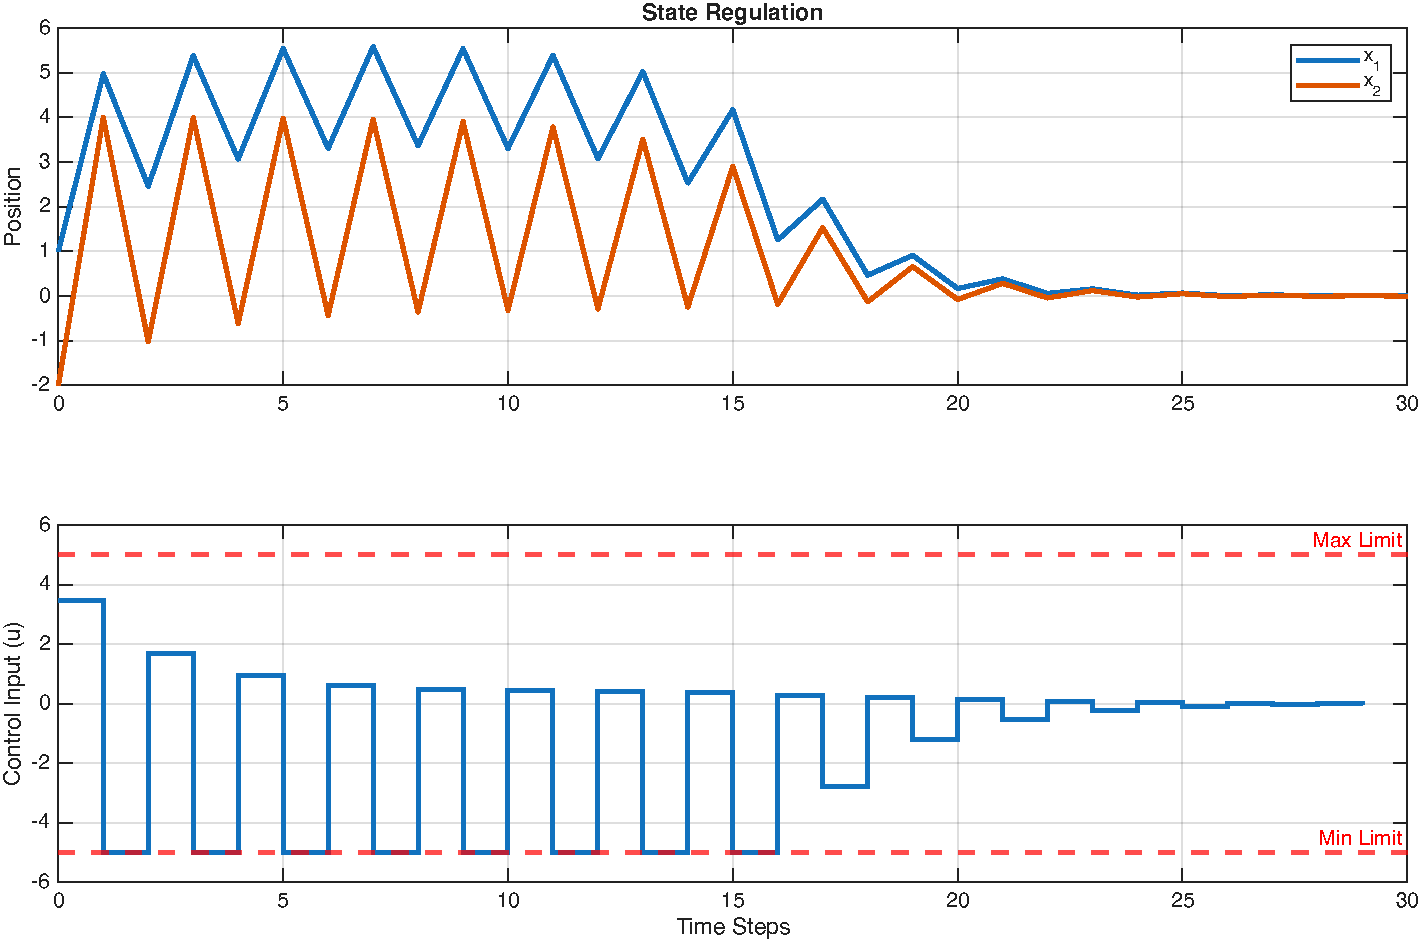
\includegraphics[width=0.7\linewidth]{Figures/Simple_MPC}
	\captionof{figure}{\emph{MPC Regulation of an Unstable Oscillatory System.}
		The top plot displays the state trajectories starting from $x_0 = [1; -2]^\top$. The characteristic "zig-zag" behaviour is caused by the negative eigenvalue $\lambda = -1.5$, while the instability drives the amplitude growth. 
		The bottom plot shows the control effort. The MPC controller effectively "clamps" the input to the constraint boundary ($u_{\min} = -5$) for the first 16 steps to counteract the unstable dynamics. Once the system energy is sufficiently reduced (around $t=18$), the control signal enters the linear region and smoothly drives the states to the origin.}
	\label{fig:simplempc}
\end{center}

\end{examplebox}

\section{The Effect of Horizon ($N$) and Terminal Cost ($P$)}
\label{sec:effect_of_N}

A common pitfall in MPC design is choosing parameters that make the controller "myopic" (short-sighted). If the horizon $N$ is too short, the controller may not see the approaching constraints or the equilibrium point in time to stop, leading to instability.

We can solve this problem in two ways:
\begin{enumerate}
	\item \textbf{Increase $N$:} This extends the controller's vision, but increases computational complexity linearly (or polynomially, depending on the solver). Typically it would be reasonable to choose 
	\begin{equation*}
		N \cdot T_s \approx T_\text{settling}
	\end{equation*}
	This selection is dependent on $T_\text{sampling}$. 	In other words, we aim to have approximately $10$ to $20$ samples during the rising phase of the step response:
	\begin{equation*}
		T_\text{sampling} \approx \frac{T_r}{10} \quad \text{to} \quad \frac{T_r}{20}
	\end{equation*}
	where $T_r$ is the rise time of the system that is controlled. Hence, 
		\begin{equation*}
		N \approx 20 \text{--} 50 \text{ samples}
	\end{equation*}

	\item \textbf{Add Terminal Cost $P$:} This adds an "artificial" cost to the end of the horizon. By setting $P$ equal to the infinite-horizon LQR cost, we trick the controller into thinking it plans for eternity, even if $N$ is small.
\end{enumerate}

While short horizons can lead to instability, a more common issue in practice is \emph{Performance Degradation}. If the control authority is "expensive" (high $R$) and the horizon is short, the controller becomes "lazy."

\begin{figure}[h]
	\centering
	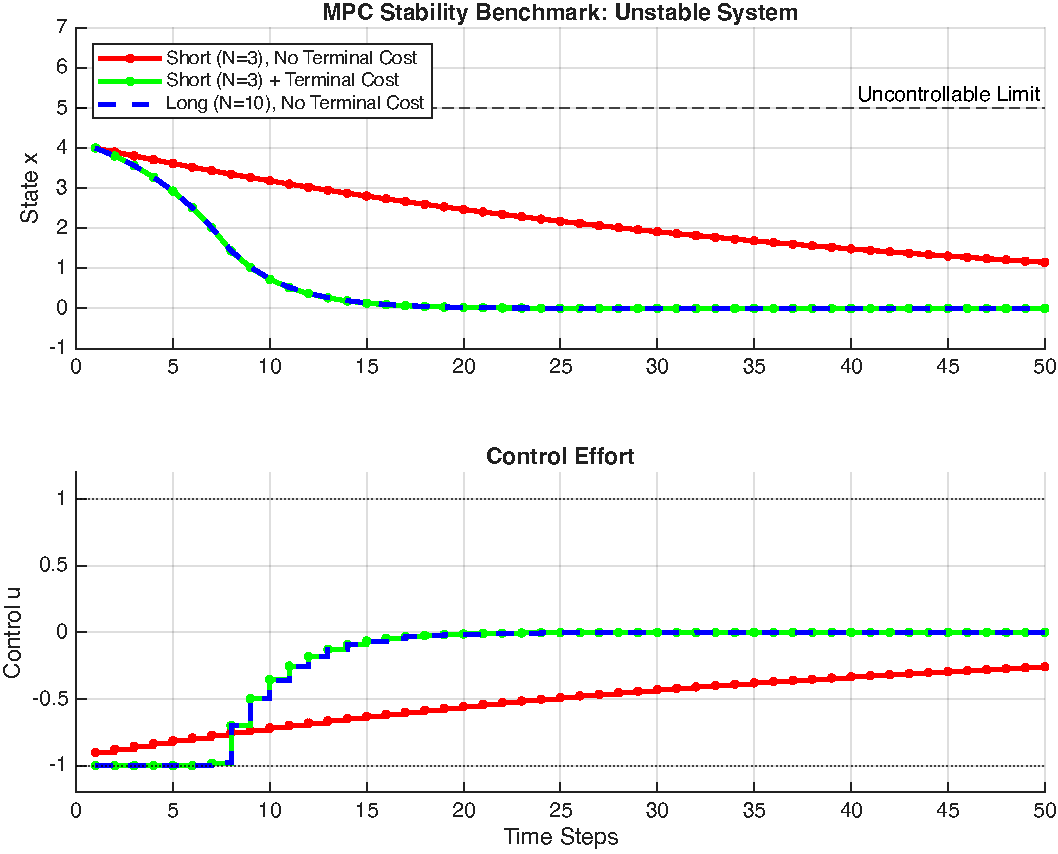
\includegraphics[width=0.9\linewidth]{Figures/Effect_of_N.pdf} 
	\caption{\emph{Performance Degradation with Short Horizons.} The system starts at $x_0=4$ with expensive control ($R=10$). The Short Horizon controller (Red) tries to save control effort in the short term as it cannot see long enough, leading to extremely slow convergence. The Terminal Cost controller (Green) recognises the long-term value of aggressive action, matching the performance of the Long Horizon controller (Blue).}
	\label{fig:mpc_lazy}
\end{figure}

\begin{examplebox}{MATLAB Benchmark: Stability Analysis}
	To rigorously test the stability properties of the MPC controller, we utilise an \emph{open-loop unstable scalar system}.
	
	\textbf{1. The Experiment:}
	We define an unstable system subject to strict input constraints:
	\begin{equation*}
		x_{k+1} = 1.2 x_k + u_k, \qquad -1 \leq u_k \leq 1
	\end{equation*}
	The initial condition $x_0 = 4$ is chosen close to the controllability limit. We compare three controller configurations:
	\begin{enumerate}
		\item \textbf{Short Horizon ($N=3$):} A very myopic controller.
		\item \textbf{Long Horizon ($N=10$):} A far-sighted controller.
		\item \textbf{Short Horizon with $P$ ($N=3, P=P_{LQR}$):} A myopic controller compensated with a terminal cost.
	\end{enumerate}
	
	\textbf{2. The Results (see Figure \ref{fig:mpc_lazy}):}
	\begin{itemize}
		\item \textbf{The Lazy Controller (Red Line):} 
		With $N=3$ and no terminal cost, the controller minimises the cost over a very short window. It calculates that applying maximum braking ($u=-1$) is \emph{too expensive} ($R=10$) relative to the short-term reduction in state error. It chooses a "soft" braking strategy ($u \approx -0.9$). While this prevents immediate explosion, convergence is very slow. The controller fails to realise that dragging out the error over a long time will result in a much higher \textit{total} cost.
		
		\item \textbf{The Optimal Controller (Green/Blue Lines):} 
		By adding the Terminal Cost ($P$) or extending the horizon ($N=10$), the controller accounts for the \emph{infinite tail} of the cost function. It realises that while braking hard ($u=-1$) is expensive \textit{now}, it is the only way to minimise the sum of squared errors over the long run. Consequently, it acts aggressively, driving the state to zero in minimal time.
	\end{itemize}
	
	\textbf{Conclusion:} The Terminal Cost $P$ is not just a stability anchor; it is a crucial tuning parameter that restores \emph{long-term optimality} to short-horizon controllers.
\end{examplebox}

% ================================================================
% FORMAL STABILITY THEORY
% ================================================================
\section{Recursive Feasibility and Formal Stability Guarantees\texorpdfstring{$^{(*)}$}{(*)}}
\label{sec:mpc_stability_theory}

The previous sections showed experimentally that adding the terminal cost $P$ improves MPC performance and can prevent instability. We now explain \textit{why} this works, and what additional ingredient is needed to \textit{guarantee} stability rigorously.

\subsection{The Gap in the Argument}

Consider the MPC cost function:
\[
J = \sum_{k=0}^{N-1} \bigl(x_k^\top Q\, x_k + u_k^\top R\, u_k\bigr) + x_N^\top P\, x_N
\]
The terminal cost $x_N^\top P\, x_N$ is supposed to represent the cost of controlling the system from $x_N$ to the origin \textit{after} the horizon ends. This representation is exact when the LQR controller $u = -Kx$ is applied from step $N$ onward \emph{and no constraints are violated} during that infinite tail.

But nothing in the formulation above prevents $x_N$ from landing in a region where the LQR input $-Kx_N$ would violate the constraint $|u| \le u_{\max}$. If that happens, the terminal cost $P$ is wrong --- it promises a future cost that cannot actually be achieved without breaking the constraints.

This is not only a theoretical concern. When $x_N$ is large and the constraints are tight, the MPC may plan a trajectory that looks optimal over the $N$-step window but leads to constraint violations (or solver infeasibility) at the very next time step.

To close this gap, we need two things:
\begin{enumerate}
	\item A \emph{terminal set} $\mathcal{X}_f$ --- a region of the state space where the LQR controller can operate indefinitely without violating any constraint.
	\item A \emph{terminal constraint} $x_N \in \mathcal{X}_f$ added to the MPC optimisation, which forces the predicted terminal state to land inside this safe region.
\end{enumerate}

\subsection{Positive Invariant Sets}

The terminal set $\mathcal{X}_f$ must have a very specific property: once the state enters $\mathcal{X}_f$, the LQR controller must keep it there forever, while satisfying all constraints at every future step. A set with this property is called \emph{positively invariant}.

\begin{defnbox}{Definition: Positive Invariant Set}
	A set $\mathcal{X}_f \subseteq \mathbb{R}^n$ is a \emph{positive invariant set} for the closed-loop system $x_{k+1} = (A - BK)\,x_k$ under the terminal control law $u = -Kx$, subject to constraints $u \in \mathcal{U}$, $x \in \mathcal{X}$, if for every state $x \in \mathcal{X}_f$ the following three conditions hold:
	\begin{enumerate}[noitemsep]
		\item The input $u = -Kx$ satisfies the input constraints: $-Kx \in \mathcal{U}$.
		\item The next state satisfies the state constraints: $(A - BK)x \in \mathcal{X}$.
		\item The next state stays in the set: $(A - BK)x \in \mathcal{X}_f$.
	\end{enumerate}
\end{defnbox}

Think of $\mathcal{X}_f$ as a \textit{safe harbour}. The MPC controller must steer the state into $\mathcal{X}_f$ by the end of the prediction horizon. Once the state is inside, the LQR controller takes over and handles everything from that point on --- no constraint violations, no instability, guaranteed convergence to the origin.

\subsection{Computing $\mathcal{X}_f$: A Scalar Example}
\label{subsec:terminal_set_scalar}

We compute $\mathcal{X}_f$ step by step for the scalar system used throughout this chapter.

\textbf{System:} $x_{k+1} = 1.2\,x_k + u_k$, with input constraint $|u_k| \le 1$.

\textbf{Step 1 --- Find the LQR gain.}
Solving the DARE with $Q = 1$, $R = 1$ gives $P \approx 1.95$ and:
\[
K = \frac{a P b}{R + b^2 P} = \frac{1.2 \times 1.95}{1 + 1.95} \approx 0.79
\]
The terminal controller is $u = -Kx \approx -0.79\,x$, and the closed-loop eigenvalue is:
\[
a_{cl} = a - bK = 1.2 - 0.79 = 0.41
\]
Since $|0.41| < 1$, the closed-loop system under LQR is stable.

\textbf{Step 2 --- Find the largest interval where the input constraint holds.}
The LQR input is $u = -Kx$. The constraint $|u| \le 1$ becomes $|Kx| \le 1$, which gives:
\[
|x| \le \frac{1}{K} = \frac{1}{0.79} \approx 1.27
\]
So the candidate terminal set is $\mathcal{X}_f = \{x : |x| \le 1.27\}$.

\textbf{Step 3 --- Verify positive invariance.}
Take any $x$ inside $\mathcal{X}_f$, so $|x| \le 1.27$. Under the LQR controller, the next state is:
\[
|x^+| = |a_{cl} \cdot x| = 0.41 \times |x| \le 0.41 \times 1.27 = 0.52
\]
Since $0.52 < 1.27$, the next state is well inside $\mathcal{X}_f$. The set is positively invariant.

In fact, the state \textit{contracts} by a factor of $0.41$ at each step inside $\mathcal{X}_f$. After entering the safe harbour, the system converges to zero quickly under the LQR controller.

\begin{notebox}{Why does this work?}
	The key is that the closed-loop eigenvalue satisfies $|a_{cl}| < 1$. This means $|x^+| < |x|$ for any non-zero $x$, so the state always shrinks. And because the boundary of $\mathcal{X}_f$ is defined by the constraint $|Kx| = 1$, the shrinking state can never reach the boundary again once it moves inward. The constraints remain satisfied at every future step.

	If the system also had state constraints $|x| \le x_{\max}$, we would need $\mathcal{X}_f \subseteq \{x : |x| \le x_{\max}\}$. For the example above, $1.27 < x_{\max}$ is required.
\end{notebox}

\subsection{The Complete MPC Problem with Terminal Constraint}

We now modify the MPC formulation from Section~\ref{sec:mpc_formulation} by adding the terminal constraint. The optimisation becomes:

\begin{align*}
	\min_{u} \quad & J = x_N^\top P\, x_N + \sum_{k=0}^{N-1} \bigl(x_k^\top Q\, x_k + u_k^\top R\, u_k\bigr) \\
	\text{s.t.} \quad & x_{k+1} = Ax_k + Bu_k, \quad k = 0, \ldots, N-1 \\
	& u_{\min} \le u_k \le u_{\max}, \quad k = 0, \ldots, N-1 \\
	& x_{\min} \le x_k \le x_{\max}, \quad k = 1, \ldots, N \\
	& {x_N \in \mathcal{X}_f}
\end{align*}

The only difference from before is the last line. This extra constraint restricts where the prediction horizon is allowed to end. The QP becomes slightly more constrained, but in return it provides a formal stability guarantee.

For the scalar case, $x_N \in \mathcal{X}_f$ simply means $|x_N| \le 1/K$. For multi-state systems, $\mathcal{X}_f$ is typically a polytope (a region defined by linear inequalities), and the constraint $x_N \in \mathcal{X}_f$ adds a set of linear inequalities to the QP --- so it remains a QP.

\subsection{Recursive Feasibility}

A controller is useless if it can solve the optimisation at time $t$ but not at time $t+1$. We need the guarantee that once the MPC problem is feasible, it \textit{stays} feasible forever. This property is called \emph{recursive feasibility}.

\begin{defnbox}{Definition: Recursive Feasibility}
	The MPC problem is \emph{recursively feasible} if, whenever a feasible solution exists at time $t$, a feasible solution also exists at time $t+1$ after applying the optimal input $u_0^\star$ to the plant.
\end{defnbox}

The proof uses a simple but powerful idea called the \emph{shifted sequence}.

\textbf{Setup.} Suppose at time $t$, the MPC solver returns the optimal input sequence:
\[
u^\star = \{u_0^\star,\; u_1^\star,\; \ldots,\; u_{N-1}^\star\}
\]
with predicted states $\{x_0, x_1, \ldots, x_N\}$, where $x_N \in \mathcal{X}_f$ (the terminal constraint is satisfied).

We apply $u_0^\star$ to the plant. The system moves to $x_1$.

\textbf{Constructing a feasible candidate at time $t+1$.}
At the next time step, we need \textit{some} feasible input sequence starting from $x_1$. We do not need the optimal one --- any feasible sequence proves that the problem has a solution. The optimiser will then find an even better one.

Here is our candidate:
\[
\tilde{u} = \{u_1^\star,\; u_2^\star,\; \ldots,\; u_{N-1}^\star,\; \underbrace{-K x_N}_{\text{LQR input at } x_N}\}
\]
We take the old optimal sequence, drop $u_0^\star$ (already used), shift everything one step to the left, and append the LQR input $-Kx_N$ at the end.

\textbf{Why is this candidate feasible?}
\begin{itemize}
	\item \textbf{Inputs $u_1^\star, \ldots, u_{N-1}^\star$:} These satisfied the constraints in the original problem, so they still do.
	\item \textbf{Predicted states $x_2, x_3, \ldots, x_N$:} These are the same states from the original prediction (the dynamics are deterministic). They satisfied the state constraints before, so they still do.
	\item \textbf{The appended input $-Kx_N$:} Since $x_N \in \mathcal{X}_f$ and $\mathcal{X}_f$ is positively invariant, the LQR input $-Kx_N$ satisfies the input constraints (by condition 1 of the definition).
	\item \textbf{The new terminal state $\tilde{x}_N = (A - BK)x_N$:} Since $x_N \in \mathcal{X}_f$ and the set is positively invariant, $(A - BK)x_N \in \mathcal{X}_f$ (by condition 3). So the terminal constraint is satisfied.
\end{itemize}

Every constraint is met. The candidate $\tilde{u}$ is feasible. The solver is guaranteed to find a solution (possibly a better one), so the MPC problem will never become infeasible.

\begin{alertbox}{The role of each ingredient}
	Remove any one ingredient and the argument breaks down:
	\begin{itemize}[noitemsep]
		\item \textbf{Without $\mathcal{X}_f$:} We cannot guarantee that $-Kx_N$ satisfies the input constraints.
		\item \textbf{Without the terminal constraint $x_N \in \mathcal{X}_f$:} We cannot guarantee that the appended input is feasible or that the new terminal state stays in $\mathcal{X}_f$.
		\item \textbf{Without positive invariance:} The new terminal state $(A - BK)x_N$ might leave $\mathcal{X}_f$, breaking the terminal constraint.
	\end{itemize}
\end{alertbox}

\subsection{The Stability Proof}
\label{subsec:stability_proof}

\begin{alertbox}{Assumption for stability}
The stability proof requires $Q \succ 0$ (positive definite). If $Q \succeq 0$ is only positive semi-definite, stability still holds provided $(Q^{1/2}, A)$ is detectable --- i.e.\ no unstable mode of $A$ is invisible to the cost.
\end{alertbox}

We now show that the closed-loop system is \emph{asymptotically stable}: the state converges to the origin. The argument uses the optimal cost $J^\star(x_t)$ as a \emph{Lyapunov function}.

A Lyapunov function is any function $V(x)$ that satisfies three conditions:
\begin{enumerate}[noitemsep]
	\item $V(x) > 0$ for all $x \ne 0$, and $V(0) = 0$. \hfill (Positive definite.)
	\item $V(x_{t+1}) < V(x_t)$ whenever $x_t \ne 0$. \hfill (Strictly decreasing.)
	\item $V(x) \to \infty$ as $\|x\| \to \infty$. \hfill (Radially unbounded.)
\end{enumerate}
If such a function exists, the state must converge to zero. The reasoning is straightforward: $V$ is positive and keeps decreasing, so it must converge to some limit. Since $V$ can only be zero at $x = 0$, the state must converge there too.

We claim that $V(x_t) = J^\star(x_t)$ --- the optimal MPC cost --- satisfies all three conditions.

\textbf{Condition 1: Positivity.}
Since $Q \succ 0$, any non-zero initial state incurs a strictly positive first stage cost: $J^\star(x) \ge x^\top Q\, x > 0$ for $x \ne 0$. And $J^\star(0) = 0$ because the zero sequence $u = 0$ keeps the state at zero with zero cost.

\textbf{Condition 3: Radial unboundedness.}
$J^\star(x) \ge x^\top Q\, x$, so as $\|x\| \to \infty$, $J^\star \to \infty$.

\textbf{Condition 2: Strict decrease.}
This is the main step. We must show that $J^\star(x_{t+1}) < J^\star(x_t)$.

Write $\ell(x,u) = x^\top Q\, x + u^\top R\, u$ for the stage cost, and $V_f(x) = x^\top P\, x$ for the terminal cost. At time $t$, the optimal cost is:
\[
J^\star(x_t) = \ell(x_t, u_0^\star) + \sum_{k=1}^{N-1} \ell(x_k, u_k^\star) + V_f(x_N)
\]

At time $t+1$, the state is $x_{t+1} = x_1$. We do not know the new optimal cost, but we can bound it from above using the shifted candidate $\tilde{u}$, since the optimal cost is at most the cost of any feasible sequence:
\[
J^\star(x_{t+1}) \;\le\; \underbrace{\sum_{k=1}^{N-1} \ell(x_k, u_k^\star)}_{\text{old stage costs (shifted)}} + \underbrace{\ell(x_N,\, -Kx_N) + V_f\bigl((A-BK)x_N\bigr)}_{\text{cost of the appended LQR step}}
\]

Now subtract:
\[
J^\star(x_t) - J^\star(x_{t+1}) \;\ge\; \ell(x_t, u_0^\star) + V_f(x_N) - \ell(x_N, -Kx_N) - V_f\bigl((A-BK)x_N\bigr)
\]

Here is where the choice of $P$ matters. Because $P$ is the DARE solution, it satisfies:
\[
V_f(x) = \ell(x, -Kx) + V_f\bigl((A - BK)x\bigr) \quad \text{for all } x
\]
This is exactly what the Riccati equation says in cost-to-go language: the LQR cost at state $x$ equals the current stage cost under the LQR law plus the LQR cost at the next state. Substituting $x = x_N$:
\[
V_f(x_N) - \ell(x_N, -Kx_N) - V_f\bigl((A - BK)x_N\bigr) = 0
\]

So the middle terms cancel, leaving:
\[
J^\star(x_t) - J^\star(x_{t+1}) \;\ge\; \ell(x_t, u_0^\star) \;=\; x_t^\top Q\, x_t + {u_0^\star}^\top R\, u_0^\star \;\ge\; x_t^\top Q\, x_t \;>\; 0
\]

The optimal cost decreases by at least $x_t^\top Q\, x_t$ at every step. Since $Q \succ 0$, this decrease is strictly positive whenever $x_t \ne 0$.

\begin{summarybox}{Theorem: Stability of MPC with Terminal Ingredients}
	Consider the linear system $x_{k+1} = Ax_k + Bu_k$ with constraints $u_k \in \mathcal{U}$, $x_k \in \mathcal{X}$, stage cost weights $Q \succ 0$, $R \succ 0$, and suppose:
	\begin{enumerate}[noitemsep]
		\item The terminal cost is $V_f(x) = x^\top P\, x$, where $P$ solves the DARE.
		\item The terminal controller is $\kappa_f(x) = -Kx$ (the LQR gain from the same DARE).
		\item A positive invariant set $\mathcal{X}_f$ exists for the closed-loop $(A - BK)$ under the constraints.
		\item The terminal constraint $x_N \in \mathcal{X}_f$ is included in the MPC formulation.
	\end{enumerate}
	Then:
	\begin{itemize}[noitemsep]
		\item \textbf{Recursive feasibility:} If the MPC is feasible at $t = 0$, it is feasible for all $t \ge 0$.
		\item \textbf{Asymptotic stability:} The closed-loop state converges to the origin: $x_t \to 0$ as $t \to \infty$.
		\item \textbf{Lyapunov function:} The optimal cost $J^\star(x_t)$ is non-increasing and serves as a Lyapunov function for the closed-loop system.
	\end{itemize}
\end{summarybox}

\subsection{What This Means in Practice}

The stability theorem gives a clean recipe: choose $P$ and $K$ from the DARE, compute the positive invariant set $\mathcal{X}_f$, and add the constraint $x_N \in \mathcal{X}_f$ to the QP. However, there are practical trade-offs.

\begin{itemize}
	\item \textbf{The terminal constraint shrinks the feasible region.} Only initial states from which the MPC can drive $x_N$ into $\mathcal{X}_f$ in $N$ steps are feasible. If $N$ is small or $\mathcal{X}_f$ is small, the set of feasible initial states may be too restrictive.

	\item \textbf{Increasing $N$ enlarges the feasible region.} With more steps, the controller has more room to manoeuvre the terminal state into $\mathcal{X}_f$. In the limit $N \to \infty$, the set of feasible initial states approaches the maximal controllable set.

	\item \textbf{Computing $\mathcal{X}_f$ for multi-state systems is harder.} For a scalar system, $\mathcal{X}_f$ is just an interval. For higher-dimensional systems, it is a polytope (a region defined by many linear inequalities). Algorithms exist to compute it iteratively, but the number of inequalities can grow quickly.

	\item \textbf{Many practical implementations omit the terminal constraint.} Engineers often rely on choosing $N$ large enough that $x_N$ naturally ends up near the origin, where the LQR law does not violate constraints. This is not rigorous, but it works well when the horizon covers the system's settling time ($N \cdot T_s \approx T_{\text{settling}}$, as discussed in Section~\ref{sec:effect_of_N}). The terminal cost $P$ alone provides adequate stability in most applications, even without the formal terminal set constraint.
\end{itemize}

The following table summarises the three levels of MPC design, from simplest to most rigorous:

\begin{center}
\begin{tabular}{L{3.5cm} C{2.5cm} C{2.5cm} C{3.5cm}}
	\toprule
	\textbf{Design} & \textbf{Terminal cost} & \textbf{Terminal set} & \textbf{Guarantee} \\
	\midrule
	Basic MPC & $Q_N = Q$ & None & No formal guarantee \\
	MPC with $P$ & $Q_N = P$ (DARE) & None & Works in practice; no proof \\
	Rigorous MPC & $Q_N = P$ (DARE) & $x_N \in \mathcal{X}_f$ & Recursive feasibility + stability \\
	\bottomrule
\end{tabular}
\end{center}

For most practical applications, using $Q_N = P$ with a sufficiently long horizon is the standard approach. The rigorous formulation with $\mathcal{X}_f$ is used when formal certification is required (e.g., aerospace, medical devices) or when the horizon $N$ must be kept very short for computational reasons.

\subsection{Why Terminal Set Size Matters}

The size of $\mathcal{X}_f$ directly controls the set of initial states from which MPC can find a feasible solution. Understanding this trade-off is important for controller design.

\emph{A small terminal set} means $\mathcal{X}_f$ is a tight region around the origin. The MPC must drive $x_N$ into this small target within $N$ steps, which is harder. The consequence: fewer initial states lead to a feasible problem, and a longer horizon $N$ may be needed to compensate.

\emph{A large terminal set} means $\mathcal{X}_f$ covers more of the state space. The MPC has an easier target for $x_N$, so feasibility is maintained for a wider range of initial conditions, even with a short horizon.

However, there is an upper limit: $\mathcal{X}_f$ cannot exceed the \emph{maximal positive invariant set} for the closed-loop system $(A-BK)$ under the given constraints. Any state outside this maximal set will eventually be driven to a constraint violation by the LQR controller, so it cannot belong to $\mathcal{X}_f$.

The ideal design therefore computes the largest possible $\mathcal{X}_f$ (the maximal positive invariant set), which maximises the region of attraction.

\begin{center}
	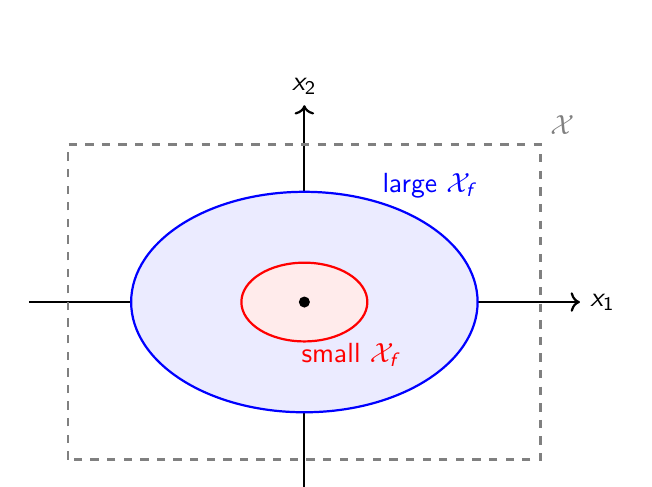
\begin{tikzpicture}[scale=1.0]
		% Axes
		\draw[->, thick] (-3.5,0) -- (3.5,0) node[right] {$x_1$};
		\draw[->, thick] (0,-2.5) -- (0,2.5) node[above] {$x_2$};
		% State constraints (outer box)
		\draw[thick, gray, dashed] (-3,-2) rectangle (3,2);
		\node[gray, anchor=south west] at (3,2) {$\mathcal{X}$};
		% Large terminal set
		\draw[thick, blue, fill=blue!8] (0,0) ellipse (2.2cm and 1.4cm);
		\node[blue, anchor=south] at (1.6,1.2) {large $\mathcal{X}_f$};
		% Small terminal set
		\draw[thick, red, fill=red!8] (0,0) ellipse (0.8cm and 0.5cm);
		\node[red, anchor=north] at (0.6,-0.4) {small $\mathcal{X}_f$};
		% Origin
		\fill (0,0) circle (2pt);
	\end{tikzpicture}
\end{center}

In the figure above, the dashed box is the state constraint set $\mathcal{X}$. With a small $\mathcal{X}_f$ (red), the MPC must work harder to hit the target. With a large $\mathcal{X}_f$ (blue), more initial states lead to feasible problems.

\subsection{Computing $\mathcal{X}_f$ for Multi-State Systems Using MPT3}

For scalar systems, we computed $\mathcal{X}_f$ by hand in the earlier example. For systems with two or more states, the terminal set is a polytope (a region bounded by many linear inequalities), and computing it by hand becomes impractical. The standard approach uses an iterative algorithm:

\begin{enumerate}
	\item Start with the constraint set: $\Omega_0 = \{x \in \mathcal{X} \mid Kx \in \mathcal{U}\}$.
	\item At each iteration, intersect with the pre-image: $\Omega_{i+1} = \Omega_i \cap \{x \mid (A-BK)x \in \Omega_i\}$.
	\item Repeat until $\Omega_{i+1} = \Omega_i$ (the set stops shrinking). This fixed point is the maximal positive invariant set $\mathcal{X}_f$.
\end{enumerate}

The iteration is guaranteed to converge in a finite number of steps for stable closed-loop systems with polytopic constraints.

In MATLAB, the \emph{Multi-Parametric Toolbox 3 (MPT3)}~\cite{Herceg2013} automates this computation. MPT3 is a free toolbox available at \texttt{https://www.mpt3.org}. The following code computes $\mathcal{X}_f$ for a two-state system:

\begin{lstlisting}[language=Matlab, caption={Computing $\mathcal{X}_f$ using MPT3}]
% System matrices
A = [1.2 1; 0 1];
B = [0.5; 1];

% Constraints
umax = 1;
xmax = [5; 5];  % state bounds: -xmax <= x <= xmax

% Step 1: Compute LQR gain and DARE solution
Q = eye(2);
R = 1;
[K_lqr, P_dare] = dlqr(A, B, Q, R);

% Closed-loop matrix under LQR
Acl = A - B*K_lqr;

% Step 2: Define constraint polytopes using MPT3
X = Polyhedron('lb', -xmax, 'ub', xmax);   % state constraints
U = Polyhedron('lb', -umax, 'ub', umax);   % input constraints

% Step 3: Build the closed-loop LTI system
sys = LTISystem('A', Acl);
sys.x.min = -xmax;
sys.x.max = xmax;

% Map input constraints through K: |K*x| <= umax
KPoly = Polyhedron('A', [K_lqr; -K_lqr], 'b', [umax; umax]);

% Step 4: Include input constraint as state constraint, then compute
X_combined = Polyhedron('A', [eye(2); -eye(2); K_lqr; -K_lqr], ...
    'b', [xmax; xmax; umax; umax]);
sys.setDomain('x', X_combined);
Xf = sys.invariantSet();

% Step 5: Visualise
figure;
plot(X, 'color', [0.9 0.9 0.9], 'alpha', 0.3); hold on;
plot(Xf, 'color', 'blue', 'alpha', 0.5);
xlabel('x_1'); ylabel('x_2');
legend('State constraints X', 'Terminal set X_f');
title('Maximal Positive Invariant Set');
\end{lstlisting}

The key function is \texttt{sys.invariantSet()}, which performs the iterative algorithm described above automatically. For the example above, the result is a polytope with several faces (linear inequalities) that can be directly used as the terminal constraint $x_N \in \mathcal{X}_f$ in the MPC formulation.

\begin{notebox}{MPT3 and YALMIP}
	MPT3 uses YALMIP internally, so both toolboxes must be installed. Once $\mathcal{X}_f$ is computed as a \texttt{Polyhedron} object, its half-space representation $H_f x \le h_f$ can be extracted with \texttt{Xf.A} and \texttt{Xf.b}, and added directly to the MPC optimisation as the linear constraint $H_f x_N \le h_f$.
\end{notebox}

\begin{notebox}{Combining MPC with State Estimation}
This chapter assumed that the full state $x_k$ is available for measurement. In practice, only noisy partial measurements $y_k = Cx_k + v_k$ are available, and the state must be estimated using a Kalman filter (Chapter~6). Chapter~8 develops the output-feedback MPC architecture that combines the estimator, a target calculator, and the MPC regulator into a complete control system.
\end{notebox}

% ================================================================
% EXPLICIT MPC
% ================================================================
\section{Explicit MPC: Solving the QP Offline\texorpdfstring{$^{(*)}$}{(*)}}
\label{sec:explicit_mpc}

Throughout this chapter, we solved the MPC optimisation problem \emph{online}: at every sampling instant, a QP solver computes $u_0^*$ before the next sample arrives. For systems with slow dynamics (sampling periods of seconds or longer), this works well. But consider a power converter switching at 100\,kHz, or a micro-electromechanical device with a 10\,$\mu$s control period. At these speeds, even a fast QP solver may not finish in time.

Explicit MPC takes a different approach: solve the MPC problem \emph{once, offline}, for every possible initial state $x_0$. The result is a \emph{piecewise affine} (PWA) control law
\[
u^*(x_0) = K_i\, x_0 + k_i \quad \text{when } x_0 \in \mathcal{R}_i
\]
where $\{\mathcal{R}_1, \mathcal{R}_2, \dots, \mathcal{R}_M\}$ is a partition of the feasible state space into polyhedral regions. At runtime, the controller determines which region contains the current state and evaluates the corresponding affine law. No optimisation, no solver --- just comparisons and arithmetic.

\subsection{Why the Optimal Law Is Piecewise Affine}

The MPC problem from Section~\ref{sec:mpc_formulation} is a QP whose data depend on the initial state $x_0$. The cost is quadratic in the decision variables $u_0, \dots, u_{N-1}$, and all constraints (dynamics, input bounds, state bounds) are linear in both $u$ and $x_0$. This makes MPC a \emph{parametric QP}: a QP parameterised by $x_0$.

At any optimal solution, the KKT conditions partition the constraints into two groups:
\begin{itemize}[nosep]
	\item \textbf{Active} (binding) --- satisfied with equality.
	\item \textbf{Inactive} --- satisfied with strict inequality.
\end{itemize}
For a fixed set of active constraints, the KKT system reduces to linear equations in $(u, x_0)$. Solving gives $u^* = K_i x_0 + k_i$, an affine function of $x_0$. This law remains valid as long as $x_0$ does not move far enough to activate a new constraint or deactivate a current one. The set of all such states forms a convex polyhedron $\mathcal{R}_i$, called a \textit{critical region}.

\begin{defnbox}{Explicit MPC Solution~\cite{Bemporad2002}}
	The optimal control law $u^*(x_0)$ of a linear MPC problem with quadratic cost is a \emph{continuous piecewise affine} function of $x_0$. The state space is partitioned into $M$ convex polyhedral \emph{critical regions} $\{\mathcal{R}_1, \dots, \mathcal{R}_M\}$, and within each region:
	\[
	u^*(x_0) = K_i\, x_0 + k_i, \qquad x_0 \in \mathcal{R}_i.
	\]
	The gains and regions $\{(K_i, k_i, \mathcal{R}_i)\}_{i=1}^M$ are computed offline by solving a \emph{multi-parametric QP (mpQP)}.
\end{defnbox}

Different active-set combinations produce different affine pieces. In one region the input constraint may be active; in an adjacent region, a state constraint takes over. The boundaries between regions are the hyperplanes where these transitions occur.

\subsection{Worked Example: Scalar System}

We return to the scalar system from Section~\ref{subsec:terminal_set_scalar}:
\[
x_{k+1} = 1.2\, x_k + u_k, \qquad |u_k| \le 1,
\]
with $Q = 1$, $R = 1$, and $N = 1$. The DARE gives $P \approx 1.95$, and the LQR gain is $K = 1.2P/(1+P) \approx 0.79$.

\begin{examplebox}{Explicit MPC for the Scalar System}

The MPC problem for a given initial state $x_0$ is:
\[
\min_{u_0}\; x_0^2 + u_0^2 + 1.95\,(1.2\, x_0 + u_0)^2
\qquad \text{s.t.} \quad -1 \le u_0 \le 1.
\]

\solution

Expanding the cost:
\[
J(u_0) = \underbrace{(1 + 1.44\,P)}_{= 3.81}\, x_0^2 + 2 \cdot 1.2\,P\, x_0\, u_0 + \underbrace{(1 + P)}_{= 2.95}\, u_0^2.
\]
This is a quadratic in $u_0$ with positive curvature. The unconstrained minimum is:
\[
\frac{\mathrm{d}J}{\mathrm{d}u_0} = 0 \quad\Longrightarrow\quad
u_0^{\text{unc}} = -\frac{1.2\,P}{1 + P}\, x_0 = -K\, x_0 \approx -0.79\, x_0.
\]
The constraint $|u_0| \le 1$ becomes active when $|Kx_0| = 1$, i.e.\ when $|x_0| = 1/K \approx 1.26$.

Three cases arise depending on where $x_0$ sits:

\textbf{Case 1: $x_0 \le -1.26$.} The unconstrained optimum $-Kx_0$ exceeds $+1$, so the upper bound constraint is active. The optimal input is $u^* = +1$ (full positive force to pull the state back).

\textbf{Case 2: $-1.26 \le x_0 \le 1.26$.} The unconstrained optimum satisfies $|u_0| \le 1$. No constraint is active. The optimal input is $u^* = -0.79\,x_0$ (identical to LQR).

\textbf{Case 3: $x_0 \ge 1.26$.} The unconstrained optimum $-Kx_0$ falls below $-1$, so the upper bound constraint is active. The optimal input is $u^* = -1$ (full negative force).

The explicit law is:
\[
u^*(x_0) = \begin{cases}
	+1 & x_0 \le -1.26 \quad (\mathcal{R}_1) \\[3pt]
	-0.79\, x_0 & |x_0| \le 1.26 \quad (\mathcal{R}_2) \\[3pt]
	-1 & x_0 \ge 1.26 \quad (\mathcal{R}_3)
\end{cases}
\]

\end{examplebox}

Figure~\ref{fig:explicit_scalar_pwa} plots this law. In $\mathcal{R}_2$, the controller behaves identically to LQR. In $\mathcal{R}_1$ and $\mathcal{R}_3$, the actuator is saturated. The breakpoints at $x_0 = \pm 1/K$ mark where the input constraint switches from inactive to active.

\begin{figure}[ht]
	\centering
	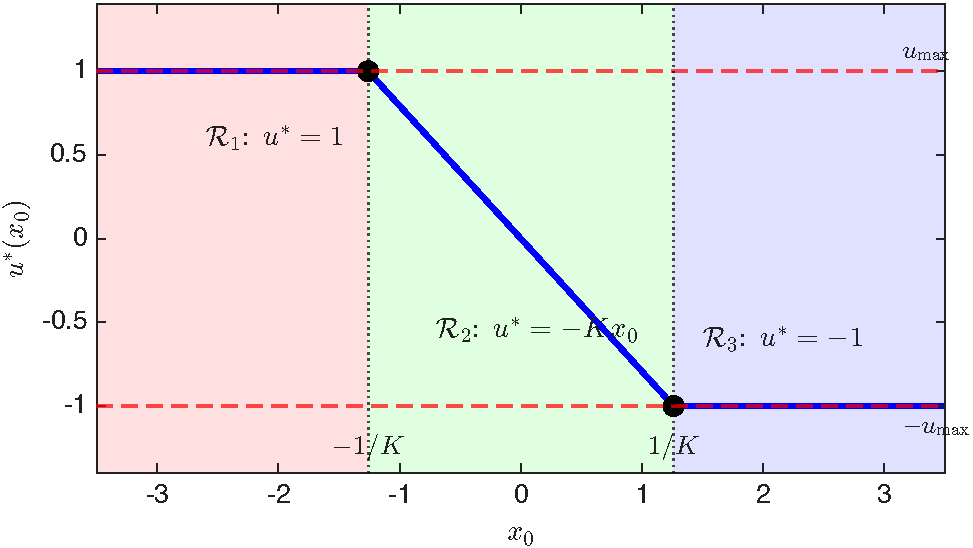
\includegraphics[width=0.85\textwidth]{Figures/fig_explicit_scalar_pwa.pdf}
	\caption{Explicit MPC law $u^*(x_0)$ for the scalar system with $|u| \le 1$, $N = 1$, $Q = R = 1$. The three critical regions correspond to: lower input constraint active ($\mathcal{R}_1$), unconstrained ($\mathcal{R}_2$), and upper constraint active ($\mathcal{R}_3$). Online evaluation requires two comparisons and one multiplication.}
	\label{fig:explicit_scalar_pwa}
\end{figure}

At runtime, the entire controller reduces to:
\begin{lstlisting}[language=Matlab, numbers=none]
if x0 <= -1.26,      u = 1;
elseif x0 >= 1.26,   u = -1;
else,                 u = -0.79 * x0;
end
\end{lstlisting}
Two comparisons and one multiply. This executes in nanoseconds on any microcontroller --- no QP solver, no YALMIP, no operating system required.

\subsection{Multi-State Systems: MPT3 Workflow}

For systems with two or more states, the critical regions are polytopes in $\mathbb{R}^n$ and must be computed algorithmically. MPT3~\cite{Herceg2013} automates the entire workflow: define the system, set up the MPC problem, and call \texttt{toExplicit()}.

We use the same double integrator as the terminal set example:
\[
A = \begin{bmatrix} 1.2 & 1 \\ 0 & 1 \end{bmatrix}, \quad B = \begin{bmatrix} 0.5 \\ 1 \end{bmatrix}, \quad |u_k| \le 1, \quad |x_{i,k}| \le 5,
\]
with $Q = I_2$, $R = 1$, $N = 5$, and the DARE terminal cost $P$.

\begin{lstlisting}[language=Matlab, caption={Computing Explicit MPC via MPT3}]
% 1. System definition
A = [1.2 1; 0 1];  B = [0.5; 1];
sys = LTISystem('A', A, 'B', B);

% 2. Constraints
sys.x.min = [-5; -5];   sys.x.max = [5; 5];
sys.u.min = -1;          sys.u.max = 1;

% 3. Cost: Q, R, terminal cost P from DARE
Q = eye(2);  R = 1;  N = 5;
[~, P] = dlqr(A, B, Q, R);
sys.x.penalty  = QuadFunction(Q);
sys.u.penalty  = QuadFunction(R);
sys.x.with('terminalPenalty');
sys.x.terminalPenalty = QuadFunction(P);

% 4. Build online MPC, then convert to explicit
mpc_online = MPCController(sys, N);
empc = mpc_online.toExplicit();
fprintf('Critical regions: %d\n', empc.nr);

% 5. Plot the polyhedral partition
figure;
empc.partition.plot();
xlabel('x_1');  ylabel('x_2');
title('Explicit MPC: Critical Regions');

% 6. Evaluate at runtime --- table lookup, no solver
x_now = [3; -1];
u_star = empc.evaluate(x_now);
fprintf('u*(x0) = %.4f\n', u_star);
\end{lstlisting}

Figure~\ref{fig:explicit_regions_2d} shows the resulting partition. Each coloured polygon is one critical region with its own affine gain $(K_i, k_i)$. The partition tiles the feasible state space without gaps or overlaps. At runtime, the controller performs a \emph{point-location query} --- testing which region contains the current state --- and evaluates $u^* = K_i x + k_i$.

\begin{figure}[ht]
	\centering
	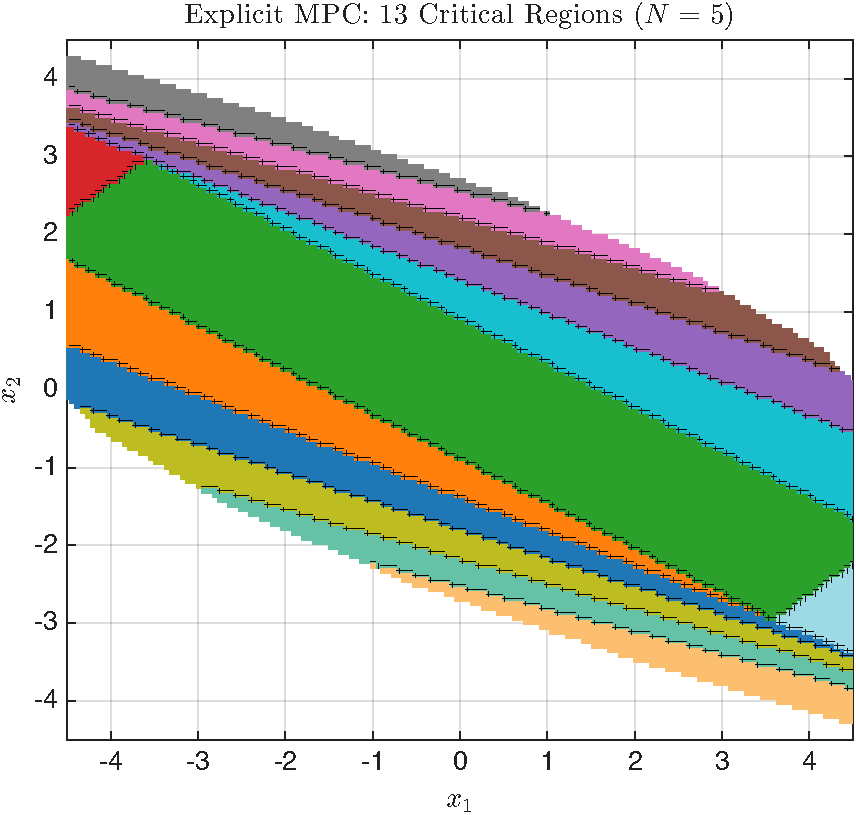
\includegraphics[width=0.75\textwidth]{Figures/fig_explicit_regions_2d.pdf}
	\caption{Polyhedral partition of the state space for the double integrator under explicit MPC with $N = 5$. Each coloured region has a distinct affine feedback gain. The partition is computed once offline; online control reduces to identifying which region contains the current state.}
	\label{fig:explicit_regions_2d}
\end{figure}

The explicit and online controllers produce \emph{identical} results --- explicit MPC is not an approximation. To verify, we simulate both controllers in closed loop from the same initial condition $x_0 = [4,\; -1]^\top$:

\begin{lstlisting}[language=Matlab, caption={Verifying explicit vs.\ online MPC equivalence}]
T_sim = 30;  x0 = [4; -1];
x_on = zeros(2, T_sim+1);  x_on(:,1) = x0;
x_ex = x_on;
u_on = zeros(1, T_sim);    u_ex = u_on;

for t = 1:T_sim
    u_on(t) = mpc_online.evaluate(x_on(:,t));   % solves QP
    x_on(:,t+1) = A*x_on(:,t) + B*u_on(t);

    u_ex(t) = empc.evaluate(x_ex(:,t));          % table lookup
    x_ex(:,t+1) = A*x_ex(:,t) + B*u_ex(t);
end
fprintf('Max |u_online - u_explicit| = %.2e\n', max(abs(u_on-u_ex)));
% Output: 1.30e-09 (numerical precision only)
\end{lstlisting}

Figure~\ref{fig:explicit_online_vs_explicit} confirms the equivalence. The state and input trajectories of both controllers overlap completely --- the red dashed line (explicit) sits exactly on top of the blue solid line (online) in all three subplots. The maximum difference in control input is $1.3 \times 10^{-9}$, i.e.\ zero to machine precision.

\begin{figure}[ht]
	\centering
	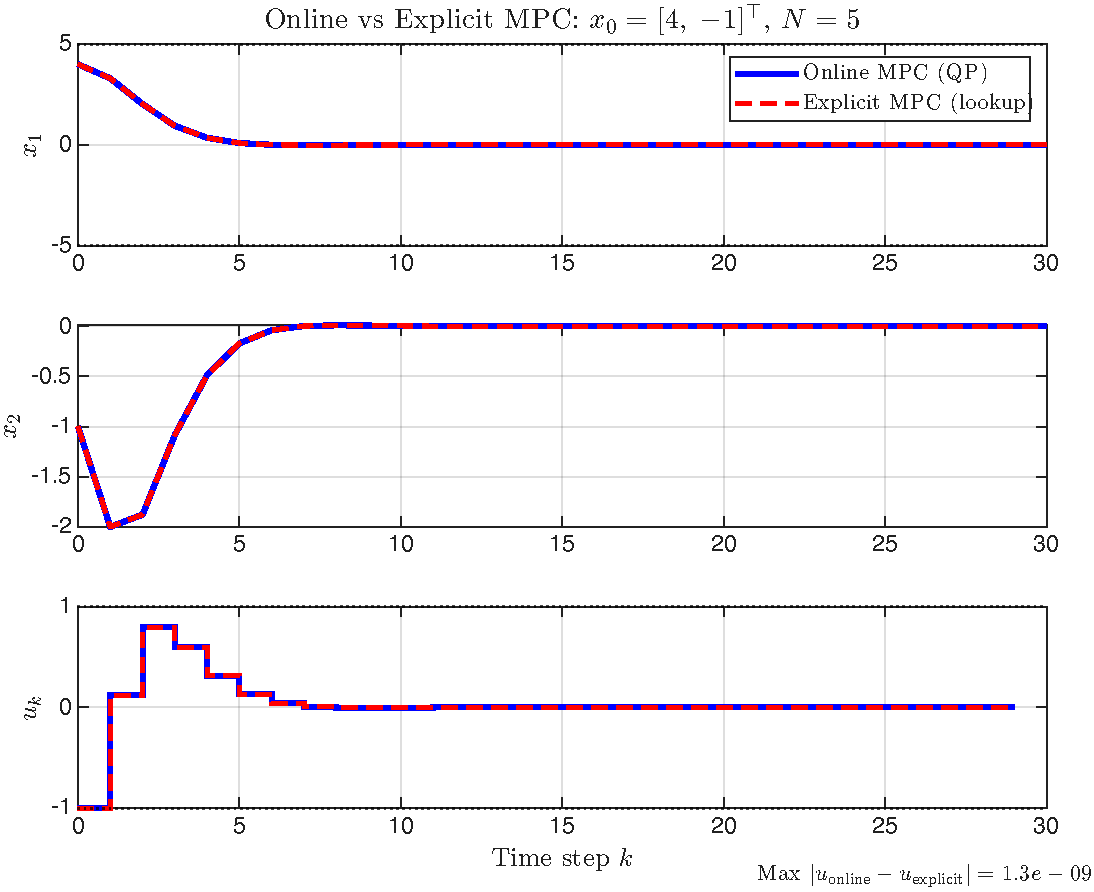
\includegraphics[width=0.9\textwidth]{Figures/fig_explicit_online_vs_explicit.pdf}
	\caption{Closed-loop comparison of online MPC (QP solved at each step) and explicit MPC (PWA lookup table) for the double integrator with $N = 5$, $x_0 = [4,\; -1]^\top$. The trajectories are indistinguishable: explicit MPC reproduces the online solution exactly.}
	\label{fig:explicit_online_vs_explicit}
\end{figure}

\subsection{The Price: Complexity Growth}

The number of critical regions $M$ determines both the offline computation time and the online storage. Each region requires storing one gain matrix $K_i \in \mathbb{R}^{n_u \times n_x}$, one offset $k_i \in \mathbb{R}^{n_u}$, and a set of half-space inequalities defining $\mathcal{R}_i$. As the system dimension, number of constraints, or prediction horizon grows, $M$ can increase rapidly.

\begin{alertbox}{Curse of dimensionality}
	The number of critical regions grows combinatorially with the problem size:
	\begin{itemize}[nosep]
		\item $n_x \le 3$, moderate $N$: tens to hundreds of regions. Practical for most embedded platforms.
		\item $n_x = 4$--$5$: thousands of regions. Feasible with care (storage in the megabyte range).
		\item $n_x \ge 6$: tens of thousands of regions or more. The offline computation may take hours and the resulting lookup table may exceed embedded memory.
	\end{itemize}
	For large systems, online QP solvers or first-order optimisation methods are preferable.
\end{alertbox}

\begin{summarybox}{Explicit MPC: When to Use It}
	\begin{center}
		\renewcommand{\arraystretch}{1.3}
		\begin{tabular}{p{0.44\textwidth} p{0.44\textwidth}}
			\toprule
			\textbf{Use explicit MPC when \dots} & \textbf{Use online MPC when \dots} \\
			\midrule
			Sampling period is very short ($\mu$s) & Sampling period allows solver time (ms--s) \\
			Few states ($n_x \le 4$) & Many states ($n_x \ge 5$) \\
			No solver available on hardware & QP solver library available \\
			Deterministic worst-case timing needed & Average-case timing acceptable \\
			Model and constraints are fixed & Model or constraints change at runtime \\
			\bottomrule
		\end{tabular}
	\end{center}
\end{summarybox}

% ================================================================
% REFERENCE TRACKING MPC
% ================================================================
\section{Reference Tracking MPC\texorpdfstring{$^{(*)}$}{(*)}}
\label{sec:tracking_mpc}

Chapters~7 and~8 focus on \emph{regulation}: driving the state to the origin, or to a constant setpoint via offset-free MPC. Many applications require the system to follow a \emph{time-varying reference trajectory} $\{x^r_k, u^r_k\}_{k=0}^{\infty}$ --- a robotic arm tracing a contour, a vehicle following a lane, or a satellite executing an orbital manoeuvre.

This section extends the MPC framework to handle trajectory tracking, including nonlinear systems for which the linearisation changes along the reference path.

\subsection{From Regulation to Tracking}

In a regulation problem, the cost penalises the state itself:
\[
J = \sum_{k=0}^{N-1} \bigl(x_k^\top Q\, x_k + u_k^\top R\, u_k\bigr) + x_N^\top P\, x_N.
\]
For tracking, we penalise the \emph{deviation} from the reference. Define:
\[
\delta x_k = x_k - x^r_k, \qquad \delta u_k = u_k - u^r_k,
\]
where $x^r_k$ and $u^r_k$ are the reference state and input at time $k$. The tracking cost becomes:
\[
J_{\text{track}} = \sum_{k=0}^{N-1} \bigl(\delta x_k^\top Q\, \delta x_k + \delta u_k^\top R\, \delta u_k\bigr) + \delta x_N^\top P\, \delta x_N.
\]

\begin{notebox}{Tracking vs.\ Offset-Free MPC (Chapter~\ref{chap:output_fb_mpc})}
	The offset-free MPC of Chapter~\ref{chap:output_fb_mpc} tracks a \emph{constant} setpoint by augmenting the model with a disturbance estimator and a target calculator. Here we address a fundamentally different problem: the reference changes at every time step, the full reference trajectory is assumed known over the prediction horizon, and no disturbance estimation is needed.
\end{notebox}

For a \emph{linear time-invariant} system $x_{k+1} = Ax_k + Bu_k$ whose reference satisfies the same dynamics ($x^r_{k+1} = Ax^r_k + Bu^r_k$), subtracting yields:
\[
\delta x_{k+1} = A\,\delta x_k + B\,\delta u_k.
\]
The tracking problem then reduces to a standard regulation problem in the deviation variables $(\delta x, \delta u)$, with the same matrices $A$ and $B$. Input constraints $u_{\min} \le u_k \le u_{\max}$ translate to:
\[
u_{\min} - u^r_k \;\le\; \delta u_k \;\le\; u_{\max} - u^r_k.
\]
The constraint bounds shift at each prediction step --- the QP structure is identical but the data changes.

\subsection{Nonlinear Tracking via Successive Linearisation}

When the plant is nonlinear,
\[
x_{k+1} = f(x_k, u_k),
\]
the deviation dynamics are no longer exactly linear. A standard approach is to \emph{linearise around the reference trajectory} at each prediction step $k$:
\begin{align*}
	A_k &= \left.\frac{\partial f}{\partial x}\right|_{x^r_k,\, u^r_k}, &
	B_k &= \left.\frac{\partial f}{\partial u}\right|_{x^r_k,\, u^r_k}.
\end{align*}
The linearised deviation dynamics become \emph{time-varying}:
\[
\delta x_{k+1} \approx A_k\,\delta x_k + B_k\,\delta u_k.
\]
At each MPC step, we solve a QP over the deviation variables with these time-varying matrices. The resulting optimisation is still a convex QP --- only the constraint and cost data change from step to step.

\begin{alertbox}{Successive Linearisation Is Not Globally Optimal}
	Each QP uses a first-order approximation of $f$ around the reference. If the actual state deviates significantly from the reference, the linearisation error grows. For large deviations, iterating the linearisation (re-linearising around the predicted trajectory rather than the reference) improves accuracy at the cost of solving multiple QPs per step. This idea---\emph{successive convexification}---is developed formally in Chapter~\ref{chap:nmpc}, alongside the full nonlinear MPC framework.
\end{alertbox}

\subsection{Application: Path Following for a Mobile Robot}

We apply tracking MPC to a nonholonomic mobile robot --- a standard platform in robotics whose motion constraints make it a natural testbed for nonlinear tracking.

\subsubsection*{The Unicycle Model}

A differential-drive robot moving on a plane has state $x = [p_x,\; p_y,\; \theta]^\top$ (position and heading) and input $u = [v,\; \omega]^\top$ (linear speed and angular rate). The continuous-time kinematics are:
\begin{align*}
	\dot{p}_x &= v\,\cos\theta, &
	\dot{p}_y &= v\,\sin\theta, &
	\dot{\theta} &= \omega.
\end{align*}
The system is nonholonomic: it cannot move sideways. Despite having three state variables, only two inputs are available, and the velocity direction is coupled to the heading through $\cos\theta$ and $\sin\theta$.

\textbf{Discretisation.} Applying Forward Euler with sampling period $T_s$:
\begin{equation*}
	\underbrace{\begin{bmatrix} p_{x,k+1} \\ p_{y,k+1} \\ \theta_{k+1} \end{bmatrix}}_{x_{k+1}}
	= \underbrace{\begin{bmatrix} p_{x,k} + T_s\, v_k \cos\theta_k \\ p_{y,k} + T_s\, v_k \sin\theta_k \\ \theta_k + T_s\, \omega_k \end{bmatrix}}_{f(x_k, u_k)}.
\end{equation*}

\textbf{Jacobians.} At a reference point $(x^r_k, u^r_k)$ with $\theta^r_k$ and $v^r_k$:
\[
A_k = \begin{bmatrix} 1 & 0 & -T_s\, v^r_k \sin\theta^r_k \\ 0 & 1 & T_s\, v^r_k \cos\theta^r_k \\ 0 & 0 & 1 \end{bmatrix}, \qquad
B_k = \begin{bmatrix} T_s \cos\theta^r_k & 0 \\ T_s \sin\theta^r_k & 0 \\ 0 & T_s \end{bmatrix}.
\]
Both matrices change along the reference path because $\theta^r_k$ and $v^r_k$ vary with $k$.

\subsubsection*{Circular Reference Trajectory}

The robot follows a circle of radius $R$ at constant speed. The reference trajectory is:
\[
x^r_k = \begin{bmatrix} R\cos(\omega_{\text{ref}}\, k T_s) \\ R\sin(\omega_{\text{ref}}\, k T_s) \\ \omega_{\text{ref}}\, k T_s + \tfrac{\pi}{2} \end{bmatrix}, \qquad
u^r_k = \begin{bmatrix} R\,\omega_{\text{ref}} \\ \omega_{\text{ref}} \end{bmatrix},
\]
where $\omega_{\text{ref}}$ is the angular rate around the circle. The reference heading is tangent to the circle (offset by $\pi/2$ from the radial direction), and the reference speed is $v^r = R\,\omega_{\text{ref}}$.

\subsubsection*{The Tracking MPC Problem}

At each time step $t$, given the current state $x_t$ and the known reference $\{x^r_{t+k}, u^r_{t+k}\}_{k=0}^{N}$, we solve:
\begin{align*}
	\min_{\delta u_0, \dots, \delta u_{N-1}} \quad & \sum_{k=0}^{N-1} \bigl(\delta x_k^\top Q\,\delta x_k + \delta u_k^\top R\,\delta u_k\bigr) + \delta x_N^\top Q\,\delta x_N \\[4pt]
	\text{s.t.} \quad
	& \delta x_0 = x_t - x^r_t \hspace{5.6cm} \text{(Initialisation)} \\
	& \delta x_{k+1} = A_k\,\delta x_k + B_k\,\delta u_k, \quad k = 0, \dots, N{-}1 \hspace{0.2cm} \text{(Linearised Dynamics)} \\
	& u_{\min} - u^r_{t+k} \le \delta u_k \le u_{\max} - u^r_{t+k} \hspace{1.95cm} \text{(Actuator Limits)}
\end{align*}
The first optimal deviation $\delta u_0^*$ is applied: $u_t = u^r_t + \delta u_0^*$.

\subsubsection*{MATLAB Implementation}

The following code implements the complete tracking MPC loop for the unicycle on a circular path.

\begin{lstlisting}[language=Matlab, caption={Tracking MPC for a nonholonomic mobile robot following a circular path.}]
% 1. Parameters
Ts = 0.1;  R_c = 3;  w_ref = 0.5;
v_ref = R_c * w_ref;  N = 15;  T_sim = 150;
Q = diag([10, 10, 2]);  Rw = diag([0.5, 0.5]);
v_min = 0;  v_max = 2.5;  w_min = -1.5;  w_max = 1.5;

% 2. Reference trajectory
t_all = (0:T_sim+N) * Ts;
xr = [R_c*cos(w_ref*t_all); R_c*sin(w_ref*t_all);
      w_ref*t_all + pi/2];
ur = repmat([v_ref; w_ref], 1, T_sim+N);

% 3. Nonlinear dynamics (Forward Euler)
f_nl = @(x,u) x + Ts*[u(1)*cos(x(3)); u(1)*sin(x(3)); u(2)];

% 4. Closed-loop simulation
x0 = [R_c+1.5; 1.0; pi/2+0.3];
x_log = zeros(3, T_sim+1);  x_log(:,1) = x0;
u_log = zeros(2, T_sim);

for t = 1:T_sim
    dx = sdpvar(3, N+1, 'full');
    du = sdpvar(2, N, 'full');

    con = [dx(:,1) == x_log(:,t) - xr(:,t)];
    obj = 0;
    for k = 1:N
        th_r = xr(3, t+k-1);  vr_k = ur(1, t+k-1);
        Ak = [1, 0, -Ts*vr_k*sin(th_r);
              0, 1,  Ts*vr_k*cos(th_r);
              0, 0,  1];
        Bk = [Ts*cos(th_r), 0; Ts*sin(th_r), 0; 0, Ts];

        con = [con, dx(:,k+1) == Ak*dx(:,k) + Bk*du(:,k)];
        con = [con, v_min-ur(1,t+k-1) <= du(1,k) <= v_max-ur(1,t+k-1)];
        con = [con, w_min-ur(2,t+k-1) <= du(2,k) <= w_max-ur(2,t+k-1)];
        obj = obj + dx(:,k)'*Q*dx(:,k) + du(:,k)'*Rw*du(:,k);
    end
    obj = obj + dx(:,N+1)'*Q*dx(:,N+1);

    optimize(con, obj, sdpsettings('verbose',0,'solver','quadprog'));
    u_log(:,t) = ur(:,t) + value(du(:,1));
    x_log(:,t+1) = f_nl(x_log(:,t), u_log(:,t));
end
\end{lstlisting}

\begin{alertbox}{Performance Note}
The code above calls \texttt{optimize} inside the simulation loop because the Jacobians $A_k$, $B_k$ change at every prediction step. This forces YALMIP to re-parse the problem at each time step, which is orders of magnitude slower than using \texttt{optimizer}. For real-time applications, one should either parameterise the Jacobians as \texttt{sdpvar} parameters or use CasADi's parametric NLP interface.
\end{alertbox}

\subsubsection*{Results}

Figure~\ref{fig:tracking_mpc_robot} shows the simulation with parameters $T_s = 0.1$\,s, $R = 3$\,m, $\omega_{\text{ref}} = 0.5$\,rad/s (one lap $\approx 12.6$\,s), $N = 15$, $Q = \operatorname{diag}(10,10,2)$, $R = \operatorname{diag}(0.5, 0.5)$.

The robot starts at $(4.5,\, 1.0)$ with heading $\theta_0 = \pi/2 + 0.3$ --- displaced from the reference circle. Within the first two seconds, the tracking MPC steers the robot onto the circular path and maintains close tracking for the remainder of the simulation. The triangular markers indicate the robot's position and heading at selected time steps.

The position errors (top-right subplot) show a transient phase during which the MPC corrects the initial offset, followed by near-zero steady-state tracking. The control inputs (bottom-right subplot) remain within the actuator limits $v \in [0,\, 2.5]$\,m/s and $\omega \in [-1.5,\, 1.5]$\,rad/s throughout.

\begin{figure}[ht]
	\centering
	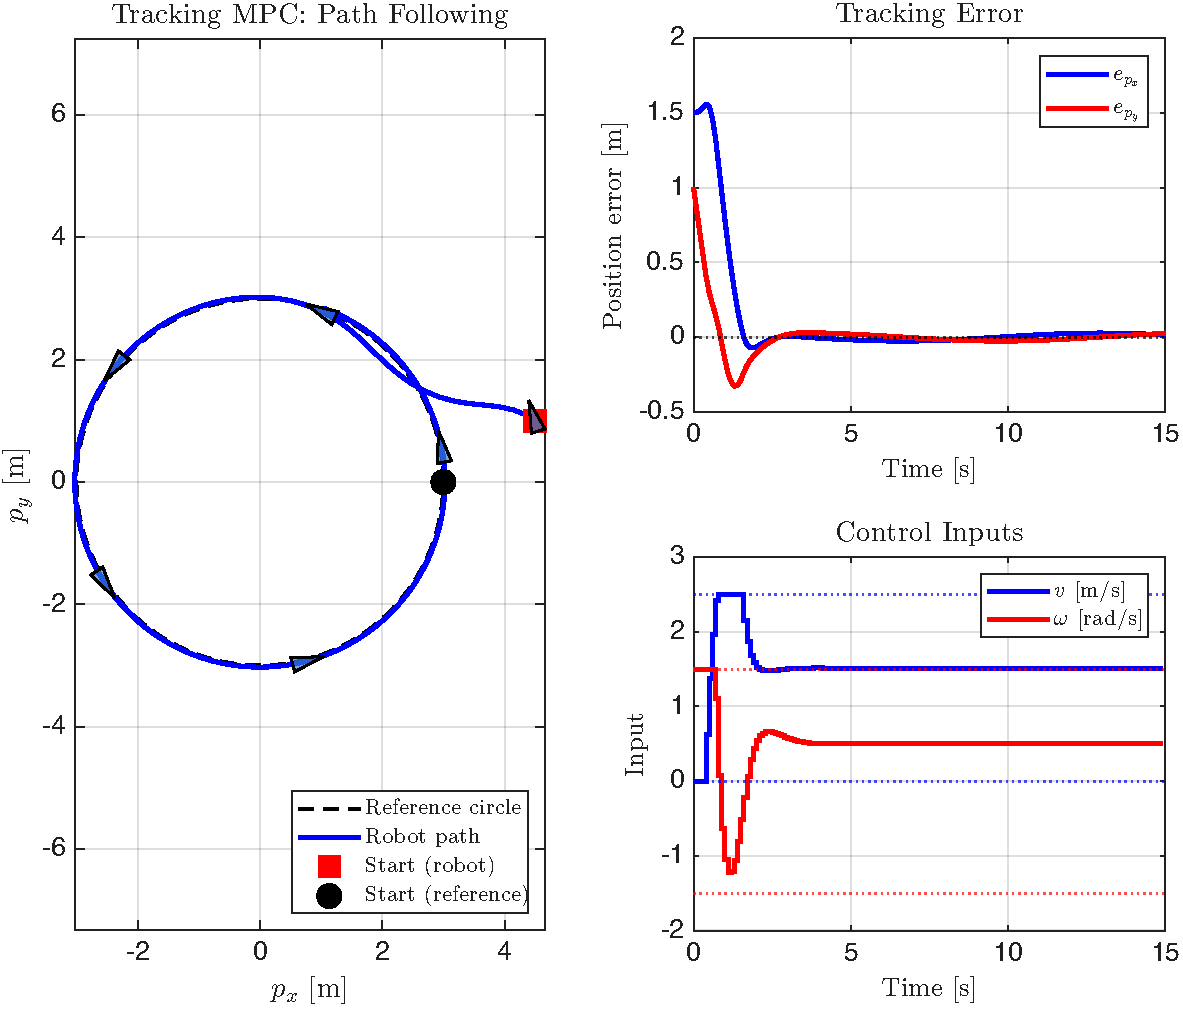
\includegraphics[width=0.95\textwidth]{Figures/fig_tracking_mpc_robot.pdf}
	\caption{Tracking MPC for a nonholonomic mobile robot following a circular path ($R = 3$\,m, $\omega_{\text{ref}} = 0.5$\,rad/s). Left: the robot (blue) converges onto the reference circle (dashed) from a displaced initial position. Top-right: position tracking errors decay to near zero. Bottom-right: linear speed $v$ and angular rate $\omega$ respect the actuator limits.}
	\label{fig:tracking_mpc_robot}
\end{figure}

\begin{summarybox}{Reference Tracking MPC}
	\begin{enumerate}[nosep]
		\item Define the reference trajectory $\{x^r_k, u^r_k\}$ over the prediction horizon.
		\item Compute deviation variables: $\delta x_k = x_k - x^r_k$, $\delta u_k = u_k - u^r_k$.
		\item For nonlinear systems, linearise $f$ around the reference at each prediction step to obtain time-varying $(A_k, B_k)$.
		\item Solve a QP in $(\delta x, \delta u)$ with shifted input constraints $u_{\min} - u^r_k \le \delta u_k \le u_{\max} - u^r_k$.
		\item Apply $u_t = u^r_t + \delta u_0^*$ to the plant. Shift the horizon and repeat.
	\end{enumerate}
\end{summarybox}

\section*{Chapter Summary}
\begin{itemize}
    \item Constrained MPC formulates the control problem as a finite-horizon optimisation with explicit inequality constraints on states and inputs.
    \item The MPC optimisation is cast as a quadratic program (QP) by substituting the predicted state trajectory in terms of the initial state and the input sequence.
    \item YALMIP provides a convenient MATLAB interface for defining decision variables, constraints, and objectives, and dispatching the resulting QP to a solver.
    \item A terminal cost term, chosen as the solution to the discrete algebraic Riccati equation (DARE), approximates the infinite-horizon cost beyond the prediction window.
    \item A terminal constraint set ensures that the state at the end of the horizon lies in a controlled-invariant region, guaranteeing recursive feasibility.
    \item Closed-loop stability is established via a Lyapunov argument showing that the optimal cost decreases at each time step under the receding-horizon policy.
    \item Explicit MPC pre-computes the optimal control law offline as a piecewise affine function of the state, enabling real-time implementation without online QP solves.
    \item Reference tracking MPC reformulates the problem in terms of deviation variables around a target steady state, allowing the controller to follow time-varying setpoints.
\end{itemize}

\section*{Exercises}
\begin{enumerate}

\item Consider the scalar system
\[
x_{k+1} = 1.5\, x_k + u_k
\]
with weighting matrices $Q = 1$, $R = 2$, and a prediction horizon $N = 2$.
\begin{enumerate}
	\item Write out the predicted states $x_1$ and $x_2$ as functions of $x_0$ and the decision variables $u_0, u_1$.
	\item Using these expressions, eliminate the states from the cost function
	\[
	J = x_2^\top Q_N\, x_2 + \sum_{k=0}^{1}\bigl(x_k^\top Q\, x_k + u_k^\top R\, u_k\bigr)
	\]
	(set $Q_N = Q$ for simplicity) and express $J$ in the standard quadratic form
	\[
	J = u^\top H\, u + 2\, x_0^\top f^\top u + \text{const.}
	\]
	where $u = [u_0 \;\; u_1]^\top$. State the matrices $H$ and $f$ explicitly.
\end{enumerate}

\item For the system
\[
x_{k+1} = 1.2\, x_k + u_k, \qquad Q = 1, \quad R = 0.5, \quad N = 1, \quad Q_N = Q,
\]
with no constraints and an initial condition $x_0 = 3$:
\begin{enumerate}
	\item Show that the MPC optimisation at $k = 0$ reduces to a single-variable unconstrained quadratic minimisation in $u_0$.
	\item Find the optimal input $u_0^\star$ and the resulting next state $x_1$.
	\item Explain why only $u_0^\star$ is applied to the plant and what happens at the next sampling instant under the receding horizon principle.
\end{enumerate}

\item Consider the same system as in Exercise~2, but now add the input constraint $-1 \le u_k \le 1$.
\begin{enumerate}
	\item For $x_0 = 3$, determine whether the unconstrained optimum $u_0^\star$ from Exercise~2 violates the constraint. If so, find the constrained optimum.
	\item Repeat for $x_0 = 10$. Simulate the closed-loop response for several steps by applying the receding horizon strategy with $N = 1$. Does the state converge to the origin?
	\item Determine (analytically or by trial) the largest initial condition $|x_0|$ for which the MPC problem with $N = 1$ and $-1 \le u_k \le 1$ remains feasible. What happens if $x_0$ exceeds this value?
\end{enumerate}

\item Consider a double integrator in discrete time:
\[
A = \begin{bmatrix} 1 & 1 \\ 0 & 1 \end{bmatrix}, \qquad B = \begin{bmatrix} 0.5 \\ 1 \end{bmatrix},
\]
with $Q = I_2$, $R = 1$, $Q_N = Q$, input constraint $-1 \le u_k \le 1$, and initial condition $x_0 = [4 \;\; 0]^\top$.
\begin{enumerate}
	\item Using YALMIP (or by hand for $N = 2$), solve the MPC problem for horizons $N = 2, 5, 10, 20$ and record the first optimal input $u_0^\star$ in each case.
	\item Simulate the closed-loop response for each horizon length over $30$ time steps. Plot the state trajectories and input sequences.
	\item Discuss how $N$ affects the speed of convergence, constraint activity, and computational cost. What is the minimum $N$ for which the closed-loop system appears stable?
\end{enumerate}

\item Return to the scalar system
\[
x_{k+1} = 1.2\, x_k + u_k, \qquad -1 \le u_k \le 1,
\]
with $Q = 1$, $R = 10$, and $x_0 = 4$.
\begin{enumerate}
	\item Solve the discrete algebraic Riccati equation to obtain the terminal cost weight $P$.
	\item Simulate the closed-loop system under MPC with $N = 3$ and $Q_N = Q$ (no terminal cost correction). Repeat with $Q_N = P$. Compare the convergence rates.
	\item Explain, using the concept of the infinite-horizon cost-to-go, why adding the terminal cost $P$ improves performance even though the horizon $N$ remains short.
	\item For the case $Q_N = P$, under what conditions is the terminal cost a valid approximation of the true cost-to-go beyond the horizon? State the role of the terminal set $\mathcal{X}_f$ and the terminal control law $u = -Kx$ in a rigorous stability proof.
\end{enumerate}

\item A control engineer designs an MPC controller for a chemical reactor modelled as
\[
x_{k+1} = A x_k + B u_k, \qquad x_k \in \mathbb{R}^3, \quad u_k \in \mathbb{R}^2,
\]
with state constraints $x_{\min} \le x_k \le x_{\max}$ representing safety limits and input constraints $u_{\min} \le u_k \le u_{\max}$ representing valve positions.
\begin{enumerate}
	\item The engineer observes that the MPC solver returns an infeasibility warning at certain operating points. List three possible causes of infeasibility and, for each, suggest a practical remedy.
	\item The engineer proposes softening the state constraints by introducing slack variables $\epsilon_k \ge 0$ and replacing $x_{\min} \le x_k \le x_{\max}$ with $x_{\min} - \epsilon_k \le x_k \le x_{\max} + \epsilon_k$, adding a penalty $\rho \|\epsilon_k\|^2$ to the cost. Explain the trade-off involved in choosing $\rho$ and why input constraints should generally \emph{not} be softened.
	\item The engineer is considering two design choices: (i)~a short horizon $N = 5$ with the DARE terminal cost $Q_N = P$, and (ii)~a long horizon $N = 50$ with $Q_N = Q$. Discuss the advantages and disadvantages of each choice in terms of closed-loop stability, computational load, and robustness to model uncertainty.
\end{enumerate}

\item \textbf{(Explicit MPC)} Consider the scalar system $x_{k+1} = 1.5\,x_k + u_k$ with $|u_k| \le 1$, $Q = 1$, $R = 0.5$.
\begin{enumerate}
	\item Solve the DARE to find $P$. Compute the LQR gain $K$ and the breakpoint $x_{\text{bp}} = 1/K$.
	\item For $N = 1$, derive the explicit MPC law $u^*(x_0)$. State each critical region and its affine law. Verify that the law is continuous at the breakpoints.
	\item Now add a state constraint $|x_k| \le 3$. For $N = 1$, the constraint $|1.5\,x_0 + u_0| \le 3$ introduces additional breakpoints. Find them and sketch the new $u^*(x_0)$.
	\item For $N = 2$ with input constraints only ($|u_k| \le 1$, no state constraint), how many possible active-set combinations exist? Use MATLAB to compute and plot $u_0^*(x_0)$. How many critical regions arise?
	\item If you have MPT3 installed, compute the explicit controller for the double integrator from Exercise~4 with horizons $N = 3, 5, 10$. Report the number of critical regions for each case and comment on the growth rate.
\end{enumerate}

\end{enumerate}


	\chapter{Output Feedback and Offset-Free MPC}
\label{chap:output_fb_mpc}

\section{Introduction}
In the previous chapter, we derived Model Predictive Control under idealised assumptions: full state measurement, a perfect model, and no disturbances. Under these pure conditions, a simple regulator is sufficient to drive the system to the origin.

However, real-world control engineering is defined by its imperfections. Sensors are noisy and limited in number, meaning that the full state is rarely measurable. Models are merely approximations, failing to capture complex phenomena such as friction, aerodynamic drag or slowly varying biases. Furthermore, disturbances are rarely \emph{zero-mean}; a drone is subject to a constant gravitational force, and a building experiences continuous solar heat gains.

If we apply a standard MPC regulator to such a system, it will generally fail to track the reference exactly. The mismatch between the model's prediction and the plant's actual behaviour results in a permanent \emph{steady-state error} (or offset).

This chapter addresses these limitations. We introduce the \emph{output-feedback} framework, replacing the assumption of full-state access with a \emph{Kalman filter} that estimates the state from noisy measurements. We then develop \emph{offset-free MPC}~\cite{Pannocchia2003}: by augmenting the system model with a \textit{disturbance state} and employing a \textit{target calculator}, the MPC gains an integral-action-like capability. Under the usual observability, feasibility and modelling assumptions, this enables zero steady-state tracking error for constant or slowly varying disturbances and references.

\begin{notebox}{Connection to Classical Control}
	In PID control, steady-state error is eliminated by adding an \emph{integrator} term \(\frac{1}{s}\). In MPC, the same effect is achieved by \emph{estimating a disturbance} \(d\). In the language of the \textit{internal model principle}, augmenting the controller with a constant-disturbance model is closely related to embedding integral action.
\end{notebox}

\section{The Disturbance Model}

Standard LQR/MPC typically models plant uncertainty through zero-mean stochastic terms such as process noise \(w_k\). However, many practically important effects behave instead like persistent biases or slowly varying loads, such as gravity acting on a drone or solar gains acting on a building.

To handle this, we augment the system model with a \emph{disturbance state} \(d_k\), assumed constant or slowly varying:
\begin{align}
	x_{k+1} &= A x_k + B u_k + B_w d_k + w_k \label{eq:aug_sys_x}\\
	d_{k+1} &= d_k + \xi_k \label{eq:aug_sys_d}\\
	y_k &= C x_k + C_d d_k + v_k \label{eq:aug_sys_y}
\end{align}
where:
\begin{itemize}
	\item \(d_k \in \mathbb{R}^{n_d}\) is the integrating disturbance state.
	\item \(B_w\) determines how the disturbance enters the state equation. A common choice is the \emph{input-disturbance model}, in which \(B_w = B\), meaning that the disturbance acts through the same channel as the control input.
	\item \(C_d\) models disturbances that affect the output directly, for example a measurement bias.
	\item \(\xi_k\) is a \emph{fictitious} process-noise term. Physically, \(d_k\) may be constant, but we allow \(\xi_k\) in the estimator design so that the Kalman filter remains responsive if the real disturbance changes slowly over time.
\end{itemize}

\section{State and Disturbance Estimation}

Since the disturbance \(d_k\) is not ordinarily measurable, it must be estimated. The key idea is to treat the unknown disturbance as an additional state variable.

We therefore define the \emph{augmented state vector}
\[
z_k = \begin{bmatrix} x_k \\ d_k \end{bmatrix},
\]
and construct the corresponding augmented system:
\[
A_{\mathrm{aug}} =
\begin{bmatrix}
	A & B_w \\
	0 & I
\end{bmatrix}, \qquad
B_{\mathrm{aug}} =
\begin{bmatrix}
	B \\
	0
\end{bmatrix}, \qquad
C_{\mathrm{aug}} =
\begin{bmatrix}
	C & C_d
\end{bmatrix}.
\]

The identity matrix in the lower-right block of \(A_{\mathrm{aug}}\) expresses the modelling assumption that the disturbance remains constant from one step to the next unless the estimator sees evidence to the contrary.

A standard Kalman filter may now be designed for the augmented system \((A_{\mathrm{aug}}, C_{\mathrm{aug}})\). 

\begin{alertbox}{Observability Condition}
	For the disturbance to be estimable, the augmented pair \((A_{\mathrm{aug}}, C_{\mathrm{aug}})\) must be observable, or at least detectable. Intuitively, the available measurements must contain enough information to distinguish a change in the physical state \(x_k\) from a change in the disturbance \(d_k\).
	
	A useful practical rule of thumb is not to introduce more independent integrating-disturbance components than can be supported by the measured outputs. Otherwise, the augmented model is likely to become unobservable.
\end{alertbox}

\section{The Target Calculator}

To achieve offset-free tracking, we cannot simply drive the input towards zero. If a disturbance \(\hat d_k\) is pushing the system, the actuators must generally maintain a non-zero steady-state input \(u_{ss}\) in order to counteract it.

We therefore compute steady-state targets by solving the equilibrium equations. At steady state we require:
\begin{enumerate}
	\item The state to remain stationary,
	\[
	x_{ss} = A x_{ss} + B u_{ss} + B_w \hat d_k,
	\]
	\item The output to match the reference,
	\[
	r_k = C x_{ss} + C_d \hat d_k.
	\]
\end{enumerate}

\subsection{Method 1: Linear Solution (Unconstrained)}

In the simplest case, where the target is reachable and no steady-state constraints are enforced, the equations above reduce to the linear system
\begin{equation} \label{eq:target_calc}
	\begin{bmatrix}
		I - A & -B \\
		C & 0
	\end{bmatrix}
	\begin{bmatrix}
		x_{ss} \\
		u_{ss}
	\end{bmatrix}
	=
	\begin{bmatrix}
		B_w \hat d_k \\
		r_k - C_d \hat d_k
	\end{bmatrix}.
\end{equation}
If the coefficient matrix is nonsingular, this yields a computationally cheap steady-state target. However, it ignores actuator and state/output constraints, and therefore does not guarantee that the resulting target is physically reachable.

\subsection{Method 2: Constrained Optimisation (Robust)}

\begin{notebox}{The Reachability Problem}
	If the linear solution produces, for example, \(u_{ss} > u_{\max}\), then the target is infeasible. Feeding an unreachable target to the MPC regulator can compromise recursive feasibility and may lead to poor performance or failure.
\end{notebox}

To handle this, we reformulate the target calculation as a constrained \textbf{steady-state optimisation} (SSO) problem. Instead of insisting on exact equality \(y_{ss}=r_k\), we minimise the tracking error whilst enforcing the equilibrium equations and any relevant constraints.

At each time step, after estimating \(\hat d_k\), we solve
\begin{align}
	\min_{x_{ss},u_{ss}} \quad &
	\|C x_{ss} + C_d \hat d_k - r_k\|_Q^2 + \|u_{ss}\|_R^2
	\label{eq:target_qp}\\
	\text{subject to:} \quad &
	(I-A)x_{ss} - B u_{ss} = B_w \hat d_k, \nonumber\\
	&
	u_{\min} \le u_{ss} \le u_{\max}, \nonumber\\
	&
	x_{\min} \le x_{ss} \le x_{\max}, \nonumber
\end{align}
or, where more appropriate, output constraints may be imposed in place of state constraints.

\textbf{Advantages:}
\begin{itemize}
	\item The MPC is always asked to track a target that exists within the admissible set.
	\item If the reference \(r_k\) is unreachable, the SSO automatically returns the closest feasible operating point.
\end{itemize}

\section{The MPC Formulation}

\begin{figure}[htbp]
	\centering
	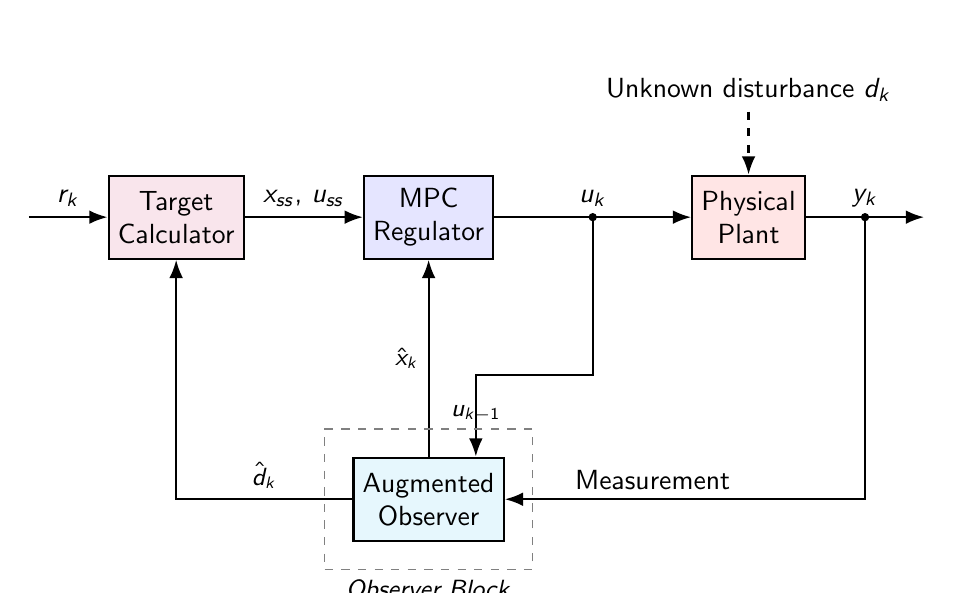
\begin{tikzpicture}[
		node distance = 1.8cm,
		auto,
		>=Latex,
		block/.style = {draw, rectangle, thick, minimum height=3em, minimum width=3.5em, align=center, fill=blue!5},
		plant/.style = {draw, rectangle, thick, minimum height=3em, minimum width=3.5em, fill=red!10, align=center},
		input/.style = {coordinate},
		output/.style = {coordinate}
		]
		
		\node [input] (input) {};
		\node [block, right=1cm of input, fill=purple!10] (target) {Target\\Calculator};
		\node [block, right=1.5cm of target, fill=blue!10] (mpc) {MPC\\Regulator};
		\node [plant, right=2.5cm of mpc] (plant) {Physical\\Plant};
		\node [output, right=1.5cm of plant] (output) {};
		
		\node [block, below=2.5cm of mpc, fill=cyan!10] (kf) {Augmented\\Observer};

		
		\draw [->, thick] (input) -- node[name=ref] {$r_k$} (target);
		\draw [->, thick] (target) -- node[above] {$x_{ss},\,u_{ss}$} (mpc);
		\draw [->, thick] (mpc) -- node[above, name=uk_node] {$u_k$} (plant);
		\draw [->, thick] (plant) -- node[name=y] (y_node) {$y_k$} (output);
		
		\node [above=0.8cm of plant] (dist) {Unknown disturbance \(d_k\)};
		\draw [->, thick, dashed] (dist) -- (plant);
		
		\draw [->, thick] (y_node.south) |- (kf.east);
		\fill (y_node.south) circle (1.5pt);
		\node at ($(mpc.south)!0.7!(plant.south) + (0, -2.8)$) {Measurement};
		
		\draw [->, thick] (kf.north) -- node[left, font=\small] {$\hat x_k$} ($(mpc.south) + (0., 0)$);
		\draw [->, thick] (kf.west) -| node[pos=0.25, above, font=\small] {$\hat{d}_k$}(target.south);
		
		\draw [->, thick] (uk_node.south) -- ++(0, -2.0) -| node[pos=0.85, above, font=\small] {$u_{k-1}$} ($(kf.north) + (0.6, 0)$);
		\fill (uk_node.south) circle (1.5pt);
		
		\node [draw=gray, dashed, inner sep=10pt, fit=(kf), label=below:\small\textit{Observer Block}] (obs_box) {};
		
	\end{tikzpicture}
	\caption{Offset-free control architecture. The target calculator uses the  disturbance estimate \(\hat d_k\) to compute the steady-state targets \((x_{ss},u_{ss})\). The MPC regulator steers the system towards these targets using the estimated state \(\hat x_k\). The augmented observer uses the measurement \(y_k\) and the previously applied control input \(u_{k-1}\). The disturbance filter is optional and is included here to reduce noise in the disturbance estimate.}
	\label{fig:offset_free_architecture}
\end{figure}

\begin{notebox}{Separation principle caveat}
The certainty-equivalence approach --- using the Kalman filter estimate $\hat{x}_k$ as if it were the true state --- is exact for unconstrained LQG. For constrained MPC, this separation no longer holds rigorously: the estimator and controller interact through the constraints. In practice, the combined observer--MPC architecture works well, but formal closed-loop guarantees require additional analysis (e.g.\ inherent robustness of MPC or robust output-feedback MPC formulations).
\end{notebox}

\begin{figure}[htbp]
	\centering
	\resizebox{\textwidth}{!}{
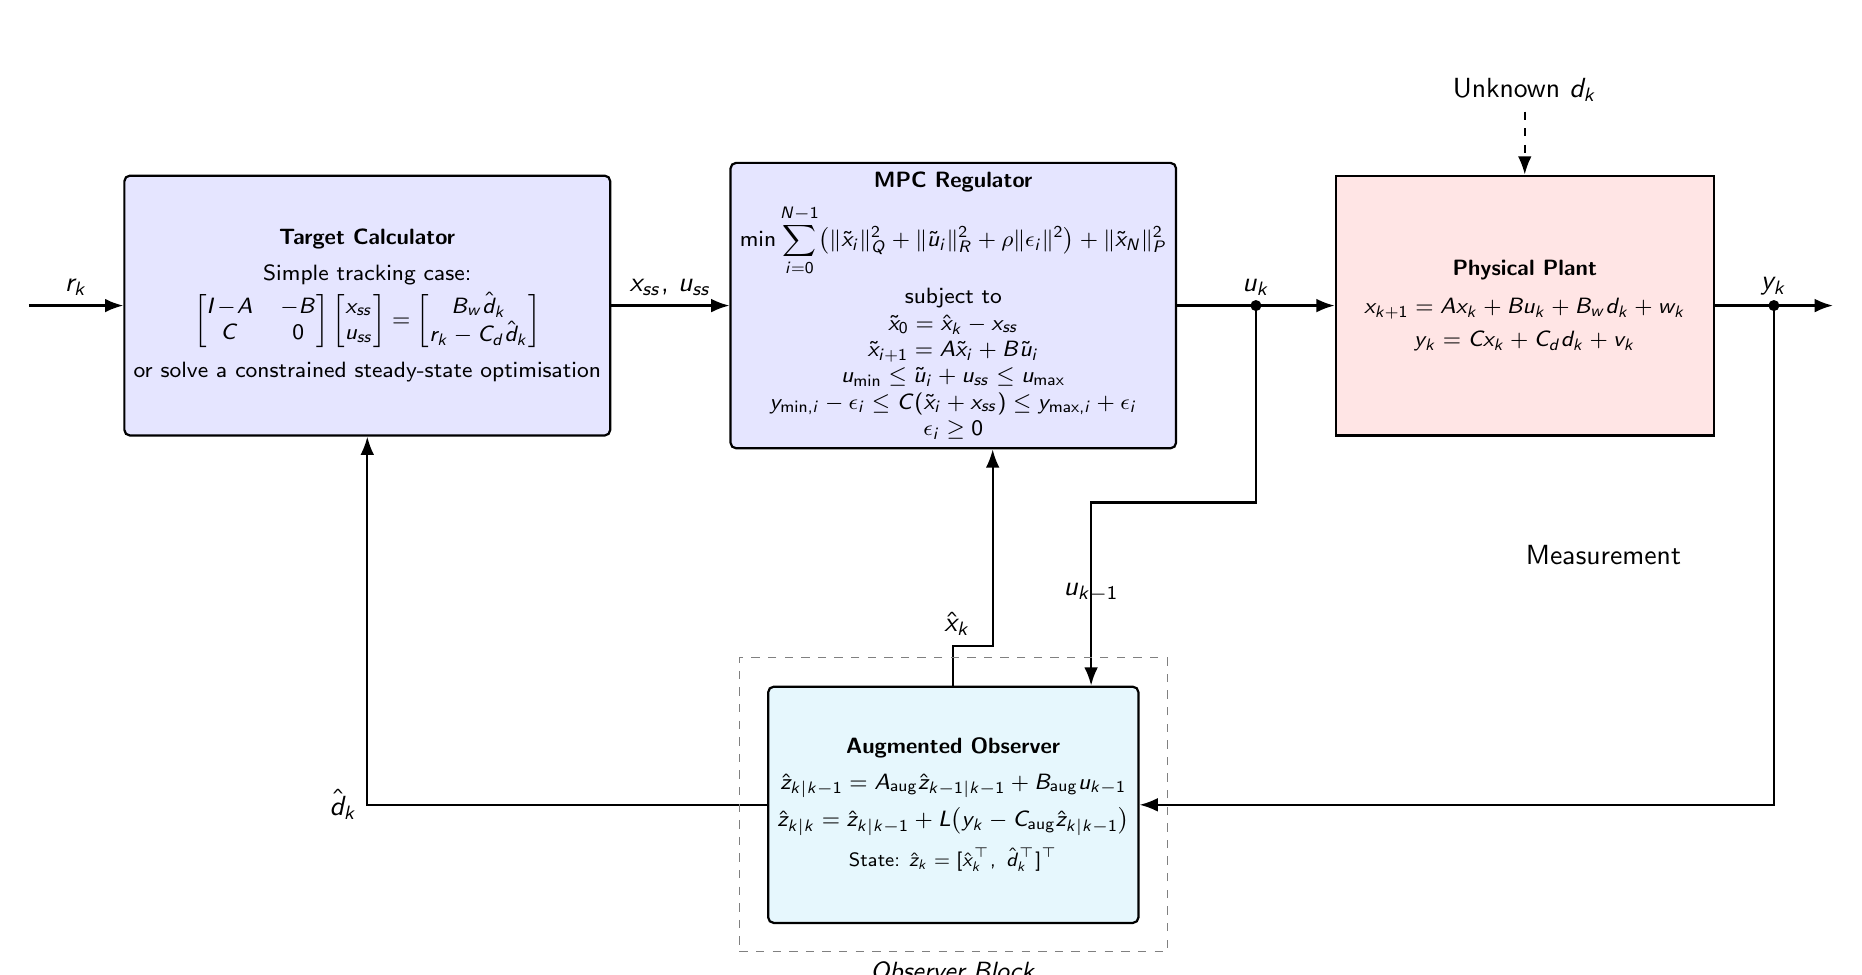
\begin{tikzpicture}[
	auto, >=Latex, node distance = 2.5cm,
	block/.style  = {draw, rectangle, thick, minimum height=3.3cm, minimum width=4.8cm,
		align=center, fill=blue!5, rounded corners=2pt, font=\footnotesize},
	plant/.style  = {draw, rectangle, thick, minimum height=3.3cm, minimum width=4.8cm,
		fill=red!10, align=center, font=\footnotesize},
	filter/.style = {draw, rectangle, thick, minimum height=3.0cm, minimum width=3.8cm,
		align=center, fill=cyan!10, rounded corners=2pt, font=\footnotesize},
	input/.style  = {coordinate},
	output/.style = {coordinate}
	]
	
	\node [input] (input) {};
	
	\node [block, right=1.2cm of input, fill=blue!10] (target) {
		\textbf{Target Calculator}\\[0.4em]
		Simple tracking case:\\[0.2em]
		\(
		\begin{bmatrix} I\!-\!A & -B\\ C & 0 \end{bmatrix}
		\begin{bmatrix} x_{ss}\\ u_{ss} \end{bmatrix}
		=
		\begin{bmatrix} B_w \hat d_k\\ r_k - C_d \hat d_k \end{bmatrix}
		\)\\[0.4em]
		or solve a constrained steady-state optimisation
	};
	
	\node [block, right=1.5cm of target, fill=blue!10] (mpc) {
		\textbf{MPC Regulator}\\[0.4em]
		\(
		\min \displaystyle\sum_{i=0}^{N-1}
		\bigl(\|\tilde x_i\|_Q^2 + \|\tilde u_i\|_R^2 + \rho\|\epsilon_i\|^2\bigr)
		+ \|\tilde x_N\|_P^2
		\)\\[0.4em]
		subject to\\
		\(\tilde x_0 = \hat x_k - x_{ss}\)\\
		\(\tilde x_{i+1} = A\tilde x_i + B\tilde u_i\)\\
		\(u_{\min} \le \tilde u_i + u_{ss} \le u_{\max}\)\\
		\(y_{\min,i}-\epsilon_i \le C(\tilde x_i+x_{ss}) \le y_{\max,i}+\epsilon_i\)\\
		\(\epsilon_i \ge 0\)
	};
	
	\node [plant, right=2.0cm of mpc] (plant) {
		\textbf{Physical Plant}\\[0.5em]
		\(x_{k+1} = A x_k + B u_k + B_w d_k + w_k\)\\[0.3em]
		\(y_k = C x_k + C_d d_k + v_k\)
	};
	
	\node [output, right=1.5cm of plant] (output) {};
	
	\node [filter, below=3cm of mpc, xshift=0cm] (kf) {
		\textbf{Augmented Observer}\\[0.4em]
		\(\hat z_{k|k-1} = A_{\mathrm{aug}}\hat z_{k-1|k-1} + B_{\mathrm{aug}}u_{k-1}\)\\[0.3em]
		\(\hat z_{k|k} = \hat z_{k|k-1} + L\!\left(y_k - C_{\mathrm{aug}}\hat z_{k|k-1}\right)\)\\[0.4em]
		{\scriptsize State: \(\hat z_k = [\hat x_k^\top,\ \hat d_k^\top]^\top\)}  % 
	};
	
	%% ── Forward path ─────────────────────────────────────────────
	\draw [->, thick] (input) -- node[name=ref] {$r_k$} (target);
	\draw [->, thick] (target) -- node[above] {$x_{ss},\,u_{ss}$} (mpc);
	\draw [->, thick] (mpc) -- node[above, name=uk_line] {$u_k$} (plant);
	\draw [->, thick] (plant) -- node[name=y] (y_node) {$y_k$} (output);
	
	\node [above=0.8cm of plant] (dist) {Unknown \(d_k\)};
	\draw [->, thick, dashed] (dist) -- (plant);
	
	%% ── Feedback paths ───────────────────────────────────────────
	\draw [->, thick] (y_node.south) |- (kf.east);
	\fill (y_node.south) circle (2pt);
	\node at ($(plant.south) + (1.0,-1.5)$) {Measurement};
	
	\draw [->, thick] (kf) -| node[left] {$\hat d_{k}$} (target);
	\draw [->, thick] (kf.north) -- ++(0,0.5)
	-| node[pos=0.05, above] {$\hat x_k$} ($(mpc.south) + (0.5,0)$);
	
	\draw [->, thick] (uk_line.south) -- ++(0,-2.5)
	-| node[pos=0.8, above] {$u_{k-1}$} ($(kf.north) + (1.75,0)$);
	\fill (uk_line.south) circle (2pt);
	
	%% ── Observer bounding box ────────────────────────────────────
	\node [draw=gray, dashed, inner sep=10pt, fit=(kf),          % ← FIX: restored full \node
	label=below:\small\textit{Observer Block}] (obs_box) {};
	
\end{tikzpicture}

	}
	\caption{Detailed offset-free control architecture. The target calculator may be implemented either as the simple linear equilibrium solve of \eqref{eq:target_calc} or, more generally, as a constrained steady-state optimisation. The regulator is shown with soft output constraints, matching the examples developed later in the chapter.}
	\label{fig:offset_free_architecture_detailed}
\end{figure}

The complete control architecture is illustrated in Figure~\ref{fig:offset_free_architecture}, with detailed mathematical definitions shown in Figure~\ref{fig:offset_free_architecture_detailed}.

\subsection{Control Topology}

The architecture operates as a hierarchical loop, separating the task of \emph{setpoint determination} from the task of \emph{regulation}. The information flow at time step \(k\) is as follows:

\begin{enumerate}
	\item \textbf{Observer Block:} The cycle begins with the measurement \(y_k\). The \emph{augmented observer} fuses this measurement with the previously applied input \(u_{k-1}\) to produce an estimate of the physical state \(\hat x_k\) and the raw disturbance estimate \(\hat d_{\mathrm{raw},k}\). To prevent high-frequency sensor noise from propagating into the controller, the disturbance estimate may be smoothed by a \emph{disturbance filter}, yielding \(\hat d_k\).
	
	\item \textbf{Target Calculator:} This block acts as the bridge between the external reference and the controller. It takes the reference \(r_k\) and the estimated disturbance \(\hat d_k\) as inputs. By solving the equilibrium equations, or more generally a constrained steady-state optimisation problem, it computes the target state \(x_{ss}\) and target input \(u_{ss}\). These represent an operating point at which the output matches the reference whilst compensating for the estimated disturbance.
	
	\item \textbf{MPC Regulator:} Finally, the MPC regulator receives the current state estimate \(\hat x_k\) together with the calculated targets \((x_{ss},u_{ss})\). Its role is to steer the system from \(\hat x_k\) towards \(x_{ss}\) whilst satisfying the imposed constraints.
\end{enumerate}

\subsection{Optimisation Problem}

Once the steady-state targets \((x_{ss}, u_{ss})\) have been computed, the
regulation layer is designed in \textbf{deviation variables}:
\[
\tilde x_i = x_i - x_{ss}, \qquad \tilde u_i = u_i - u_{ss}.
\]
The full plant prediction model at step $i$ inside the horizon follows
from~\eqref{eq:aug_sys_x} with noise terms set to zero (certainty
equivalence) and the disturbance replaced by its current estimate
$\hat d_k$:
\[
x_{i+1} = A x_i + B u_i + B_w \hat d_k.
\]
The steady-state pair $(x_{ss}, u_{ss})$ satisfies the equilibrium
condition obtained by setting $x_{k+1} = x_k = x_{ss}$ and
$d_k = \hat d_k$ in~\eqref{eq:aug_sys_x}--\eqref{eq:aug_sys_d}:
\[
x_{ss} = A x_{ss} + B u_{ss} + B_w \hat d_k,
\qquad
y_{ss} = C x_{ss} + C_d \hat d_k.
\]
Subtracting the equilibrium equation from the prediction model gives
\begin{align*}
	x_{i+1} - x_{ss}
	&= A(x_i - x_{ss}) + B(u_i - u_{ss})
	+ \underbrace{B_w \hat d_k - B_w \hat d_k}_{=\;0}.
\end{align*}
Because the steady-state pair absorbs the disturbance estimate $\hat d_k$
through both the state equation and the output equation, all affine terms
cancel exactly, leaving the \textbf{disturbance-free linear deviation
	dynamics}:
\[
\tilde x_{i+1} = A \tilde x_i + B \tilde u_i.
\]
\begin{notebox}{Notation: Real Time vs Prediction Horizon}
	MPC operates on two distinct time scales:
	\begin{itemize}
		\item \(k\) denotes the current \emph{real-time} sampling instant.
		\item \(i\) denotes the \emph{prediction step} within the horizon.
	\end{itemize}
	Thus, \(\hat x_k\) is the current estimated state, whereas \(\tilde x_i\) is the predicted deviation \(i\) steps ahead within the optimisation.
\end{notebox}

A standard offset-free tracking MPC problem is
\begin{align}
	\min_{\tilde u_0,\ldots,\tilde u_{N-1},\,\epsilon_0,\ldots,\epsilon_{N-1}} \quad &
	\sum_{i=0}^{N-1}
	\left(
	\|\tilde x_i\|_Q^2 + \|\tilde u_i\|_R^2 + \rho\|\epsilon_i\|^2
	\right)
	+ \|\tilde x_N\|_{P_{\mathrm{term}}}^2
	\label{eq:mpc_problem}\\
	\text{subject to:} \quad &
	\tilde x_0 = \hat x_k - x_{ss}, \nonumber\\
	&
	\tilde x_{i+1} = A\tilde x_i + B\tilde u_i, \qquad i=0,\ldots,N-1, \nonumber\\
	&
	u_{\min} \le \tilde u_i + u_{ss} \le u_{\max}, \nonumber\\
	&
	y_{\min,i} - \epsilon_i
	\le
	C(\tilde x_i + x_{ss})
	\le
	y_{\max,i} + \epsilon_i, \nonumber\\
	&
	\epsilon_i \ge 0, \qquad i=0,\ldots,N-1. \nonumber
\end{align}
If \(C_d \neq 0\), the corresponding term \(C_d \hat d_k\) should also be included in the predicted output equation. In the examples below, \(C_d=0\), so the simpler form above is sufficient.

\begin{notebox}{Topology Insight}
	The initialisation constraint
	\[
	\tilde x_0 = \hat x_k - x_{ss}
	\]
	is the key link between the \emph{observer} and the \emph{target calculator}. The observer supplies \(\hat x_k\), the target calculator supplies \(x_{ss}\), and the MPC regulator penalises deviations from this target.
	
	Because the cost function penalises \(\tilde x_i\) and \(\tilde u_i\) rather than the absolute input \(u_i\), the controller is not penalised for maintaining the non-zero steady-state input \(u_{ss}\) required to reject the disturbance.
\end{notebox}

The control input applied to the plant is
\[
u_k = \tilde u_0^\star + u_{ss},
\]
possibly followed by a final saturation step for numerical safety.

\subsection{Handling Infeasibility: Hard vs Soft Constraints}

In an ideal world, the MPC solver always finds a trajectory satisfying every constraint. In reality, disturbances, model mismatch or estimation errors may push the system into a region from which it is impossible to satisfy all limits simultaneously. If the feasible set becomes empty, the optimisation problem fails.

To improve robustness, it is useful to distinguish between two types of constraints.

\subsubsection*{Hard Constraints (Inputs)}
Input constraints represent immutable physical limits of the actuators, such as the maximum voltage of a motor or the fully open position of a valve. Since the controller cannot command an actuator beyond its physical capability, input constraints should normally be modelled as \emph{hard constraints}.

\subsubsection*{Soft Constraints (States/Outputs)}
State or output constraints often represent safety or performance requirements. If a large disturbance makes one of these temporarily impossible to satisfy, a hard constraint would render the optimisation infeasible exactly when corrective action is most needed. To avoid this, such constraints are often softened by introducing a slack variable.

\subsubsection*{Mathematical Implementation}
We introduce a non-negative \emph{slack variable} \(\epsilon_i \ge 0\), which acts as a safety valve for the soft constraints. Ideally, \(\epsilon_i=0\). To encourage this, we add a large penalty weight \(\rho\) to the cost function. The modified problem is
\begin{align*}
	\min_{\tilde u,\epsilon} \quad &
	\sum_{i=0}^{N-1}
	\left(
	\|\tilde x_i\|_Q^2 + \|\tilde u_i\|_R^2 + \rho\|\epsilon_i\|^2
	\right)
	+ \|\tilde x_N\|_{P_{\mathrm{term}}}^2 \\
	\text{subject to:} \quad &
	\tilde x_{i+1} = A\tilde x_i + B\tilde u_i, \\
	&
	u_{\min} \le \tilde u_i + u_{ss} \le u_{\max}, \\
	&
	y_{\min,i} - \epsilon_i
	\le
	C(\tilde x_i + x_{ss})
	\le
	y_{\max,i} + \epsilon_i, \\
	&
	\epsilon_i \ge 0.
\end{align*}

\begin{notebox}{Interpretation}
	Because \(\rho\) is chosen to be very large, the optimiser keeps \(\epsilon_i = 0\) whenever possible, so that the soft constraint behaves like a hard one. If, however, the strict bound is temporarily impossible to satisfy, the optimiser increases \(\epsilon_i\) only as much as necessary to maintain feasibility.
\end{notebox}

\begin{examplebox}{MATLAB: Offset-Free MPC with Disturbance Estimation}
	
	\textbf{Problem Formulation:}\\
	
	We consider a second-order discrete-time linear system subject to measurement noise and an unknown piecewise-constant input disturbance. The objective is to track a piecewise-constant reference \(r_k\) whilst respecting hard input constraints and soft output constraints.
	
	\textbf{System Dynamics:}\\
	
	\begin{align*}
		x_{k+1} &= A x_k + B u_k + B_w d_k \\
		y_k &= C x_k + v_k
	\end{align*}
	where the system matrices are
	\[
	A = \begin{bmatrix} 0.9535 & 0.0761 \\ -0.8454 & 0.5478 \end{bmatrix}, \quad
	B = \begin{bmatrix} 0.0465 \\ 0.8454 \end{bmatrix}, \quad
	B_w = B, \quad
	C = \begin{bmatrix} 1 & 0 \end{bmatrix}.
	\]
	
	\textbf{Constraints:}
	\begin{itemize}
		\item Hard input saturation: \(-5 \le u_k \le 5\),
		\item Soft output bounds: \(-0.5 \le y_k \le 0.5\).
	\end{itemize}
	
	\textbf{Solution Strategy:}\\
	
	A standard MPC controller based on the nominal model would exhibit a steady-state offset in the presence of the unknown disturbance. The offset-free implementation therefore uses three components:
	
	\begin{enumerate}
		\item \textbf{Augmented Kalman Filter:} The state is augmented with a constant disturbance model,
		\[
		z_k =
		\begin{bmatrix}
			x_k\\
			d_k
		\end{bmatrix}, \qquad
		z_{k+1} =
		\begin{bmatrix}
			A & B_w\\
			0 & 1
		\end{bmatrix} z_k +
		\begin{bmatrix}
			B\\
			0
		\end{bmatrix} u_k,
		\]
		and a Kalman filter provides estimates \(\hat x_k\) and \(\hat d_k\).
		
		\item \textbf{Target Calculator:} The estimated disturbance is used to compute the steady-state operating point \((x_{ss},u_{ss})\) satisfying
		\[
		(I-A)x_{ss} - B u_{ss} = B_w \hat d_k,
		\qquad
		Cx_{ss} = r_k.
		\]
		
		\item \textbf{Deviation-Form MPC:} The regulator then solves an MPC problem in deviation coordinates \(\tilde x_i = x_i - x_{ss}\), \(\tilde u_i = u_i - u_{ss}\), with soft output constraints and hard input constraints.
	\end{enumerate}
	
	\textbf{MATLAB Implementation:}\\
	
	\begin{lstlisting}[language=Matlab]
	clear; clc; close all; rng(1);
	
	%% 1. System Definition
	A  = [0.9535  0.0761; -0.8454  0.5478];
	B  = [0.0465 ; 0.8454];
	Bw = B;
	C  = [1 0];
	
	nx = 2; nu = 1; ny = 1;
	
	u_min = -5;  u_max =  5;
	y_min = -0.5; y_max =  0.5;
	
	%% 2. Augmented Observer
	% Augmented state: z_k = [x_k; d_k],  d_{k+1} = d_k
	A_aug = [A, Bw; zeros(1,nx), 1];
	B_aug = [B; 0];
	C_aug = [C, 0];
	
	% W(3,3) is the single tuning knob for disturbance tracking bandwidth
	W = diag([1e-4, 1e-4, 1e-4]);   % Kalman filter tuning weights
	V = 1e-3;                        % Measurement noise variance
	
	[P_ss, ~, ~] = dare(A_aug', C_aug', W, V);
	L = P_ss * C_aug' / (C_aug * P_ss * C_aug' + V);
	
	%% 3. Target Calculator
	% [I-A  -B] [x_ss]   [Bw * d_hat]
	% [ C    0] [u_ss] = [   ref    ]
	M_target = [eye(nx)-A, -B; C, zeros(ny,nu)];
	
	if rank(M_target) < (nx + nu)
		error('Target calculator matrix is rank deficient.');
	end
	
	%% 4. MPC Formulation
	N   = 20;
	q_y = 10;
	R   = 0.1;
	rho = 1e5;
	
	Q_state = C' * q_y * C;
	[P_N, ~, ~] = dare(A, B, Q_state, R);
	
	du    = sdpvar(nu, N,   'full');
	dx    = sdpvar(nx, N+1, 'full');
	slack = sdpvar(ny, N,   'full');
	
	x_hat = sdpvar(nx, 1);
	x_ss  = sdpvar(nx, 1);
	u_ss  = sdpvar(nu, 1);
	
	obj  = 0;
	cons = [dx(:,1) == x_hat - x_ss];
	
	for k = 1:N
		cons = [cons, dx(:,k+1) == A*dx(:,k) + B*du(:,k)];
		
		dy_k = C * dx(:,k);
		obj  = obj + dy_k'*q_y*dy_k + du(:,k)'*R*du(:,k) + rho*slack(:,k)'*slack(:,k);
		
		u_abs = du(:,k) + u_ss;
		y_abs = C * (dx(:,k) + x_ss);
		
		cons = [cons, u_min <= u_abs <= u_max];
		cons = [cons, y_min - slack(:,k) <= y_abs <= y_max + slack(:,k)];
		cons = [cons, slack(:,k) >= 0];
	end
	
	obj = obj + dx(:,N+1)' * P_N * dx(:,N+1);
	
	ops = sdpsettings('solver', 'quadprog', 'verbose', 0);
	mpc_controller = optimizer(cons, obj, ops, {x_hat, x_ss, u_ss}, {du(:,1), slack(:,1)});
	
	%% 5. Simulation Setup
	T_sim = 300;
	x_true = zeros(nx, 1);
	z_hat  = zeros(nx+1, 1);
	u_applied = 0;
	
	ref_signal = [repmat( 0.4,1,100), repmat(-0.4,1,100), repmat( 0.4,1,100)];
	w_true     = [repmat( 0.2,1,150), repmat(-0.2,1,150)];
	
	log_y_true = zeros(1,T_sim);  log_y_meas = zeros(1,T_sim);
	log_ref    = zeros(1,T_sim);  log_u      = zeros(1,T_sim);
	log_u_ss   = zeros(1,T_sim);  log_d_true = zeros(1,T_sim);
	log_d_hat  = zeros(1,T_sim);  log_slack  = zeros(1,T_sim);
	log_x1     = zeros(1,T_sim);  log_x2     = zeros(1,T_sim);
	
	fprintf('Starting simulation...\n');
	
	%% 6. Simulation Loop
	for t = 1:T_sim
	
		ref = ref_signal(t);
		
		% A. Plant output
		y_true = C * x_true;
		y_meas = y_true + sqrt(V) * randn;
		
		% B. Observer
		z_hat_pred = A_aug * z_hat + B_aug * u_applied;
		z_hat      = z_hat_pred + L * (y_meas - C_aug * z_hat_pred);
		
		x_hat_k = z_hat(1:nx);
		d_hat_k = z_hat(nx+1);
		
		% C. Target calculator
		targets = M_target \ [Bw * d_hat_k; ref];
		x_ss_k  = targets(1:nx);
		u_ss_k  = targets(nx+1:end);
		
		% D. MPC
		[sol, diagnostics] = mpc_controller{x_hat_k, x_ss_k, u_ss_k};
		
		if diagnostics == 0
			du_opt    = full(sol{1});
			slack_now = full(sol{2});
		else
			warning('MPC infeasible at t = %d (code %d). Applying u_ss.', t, diagnostics);
			du_opt    = 0;
			slack_now = NaN;
		end
		
		u_applied = min(max(du_opt + u_ss_k, u_min), u_max);
		
		% E. Plant update
		x_true = A * x_true + B * u_applied + Bw * w_true(t);
		
		% F. Logging
		log_y_true(t) = y_true;  log_y_meas(t) = y_meas;
		log_ref(t)    = ref;     log_u(t)      = u_applied;
		log_u_ss(t)   = u_ss_k;  log_d_true(t) = w_true(t);
		log_d_hat(t)  = d_hat_k; log_slack(t)  = slack_now;
		log_x1(t)     = x_true(1); log_x2(t)   = x_true(2);
	end

	
	%% Visualisation omitted for brevity.
	
	\end{lstlisting}
	Figure~\ref{fig:offset_free_results} shows the closed-loop output, the control signals, the disturbance estimate and the activity of the soft output constraint.
\end{examplebox}

\begin{figure}[!htb]
	\centering
	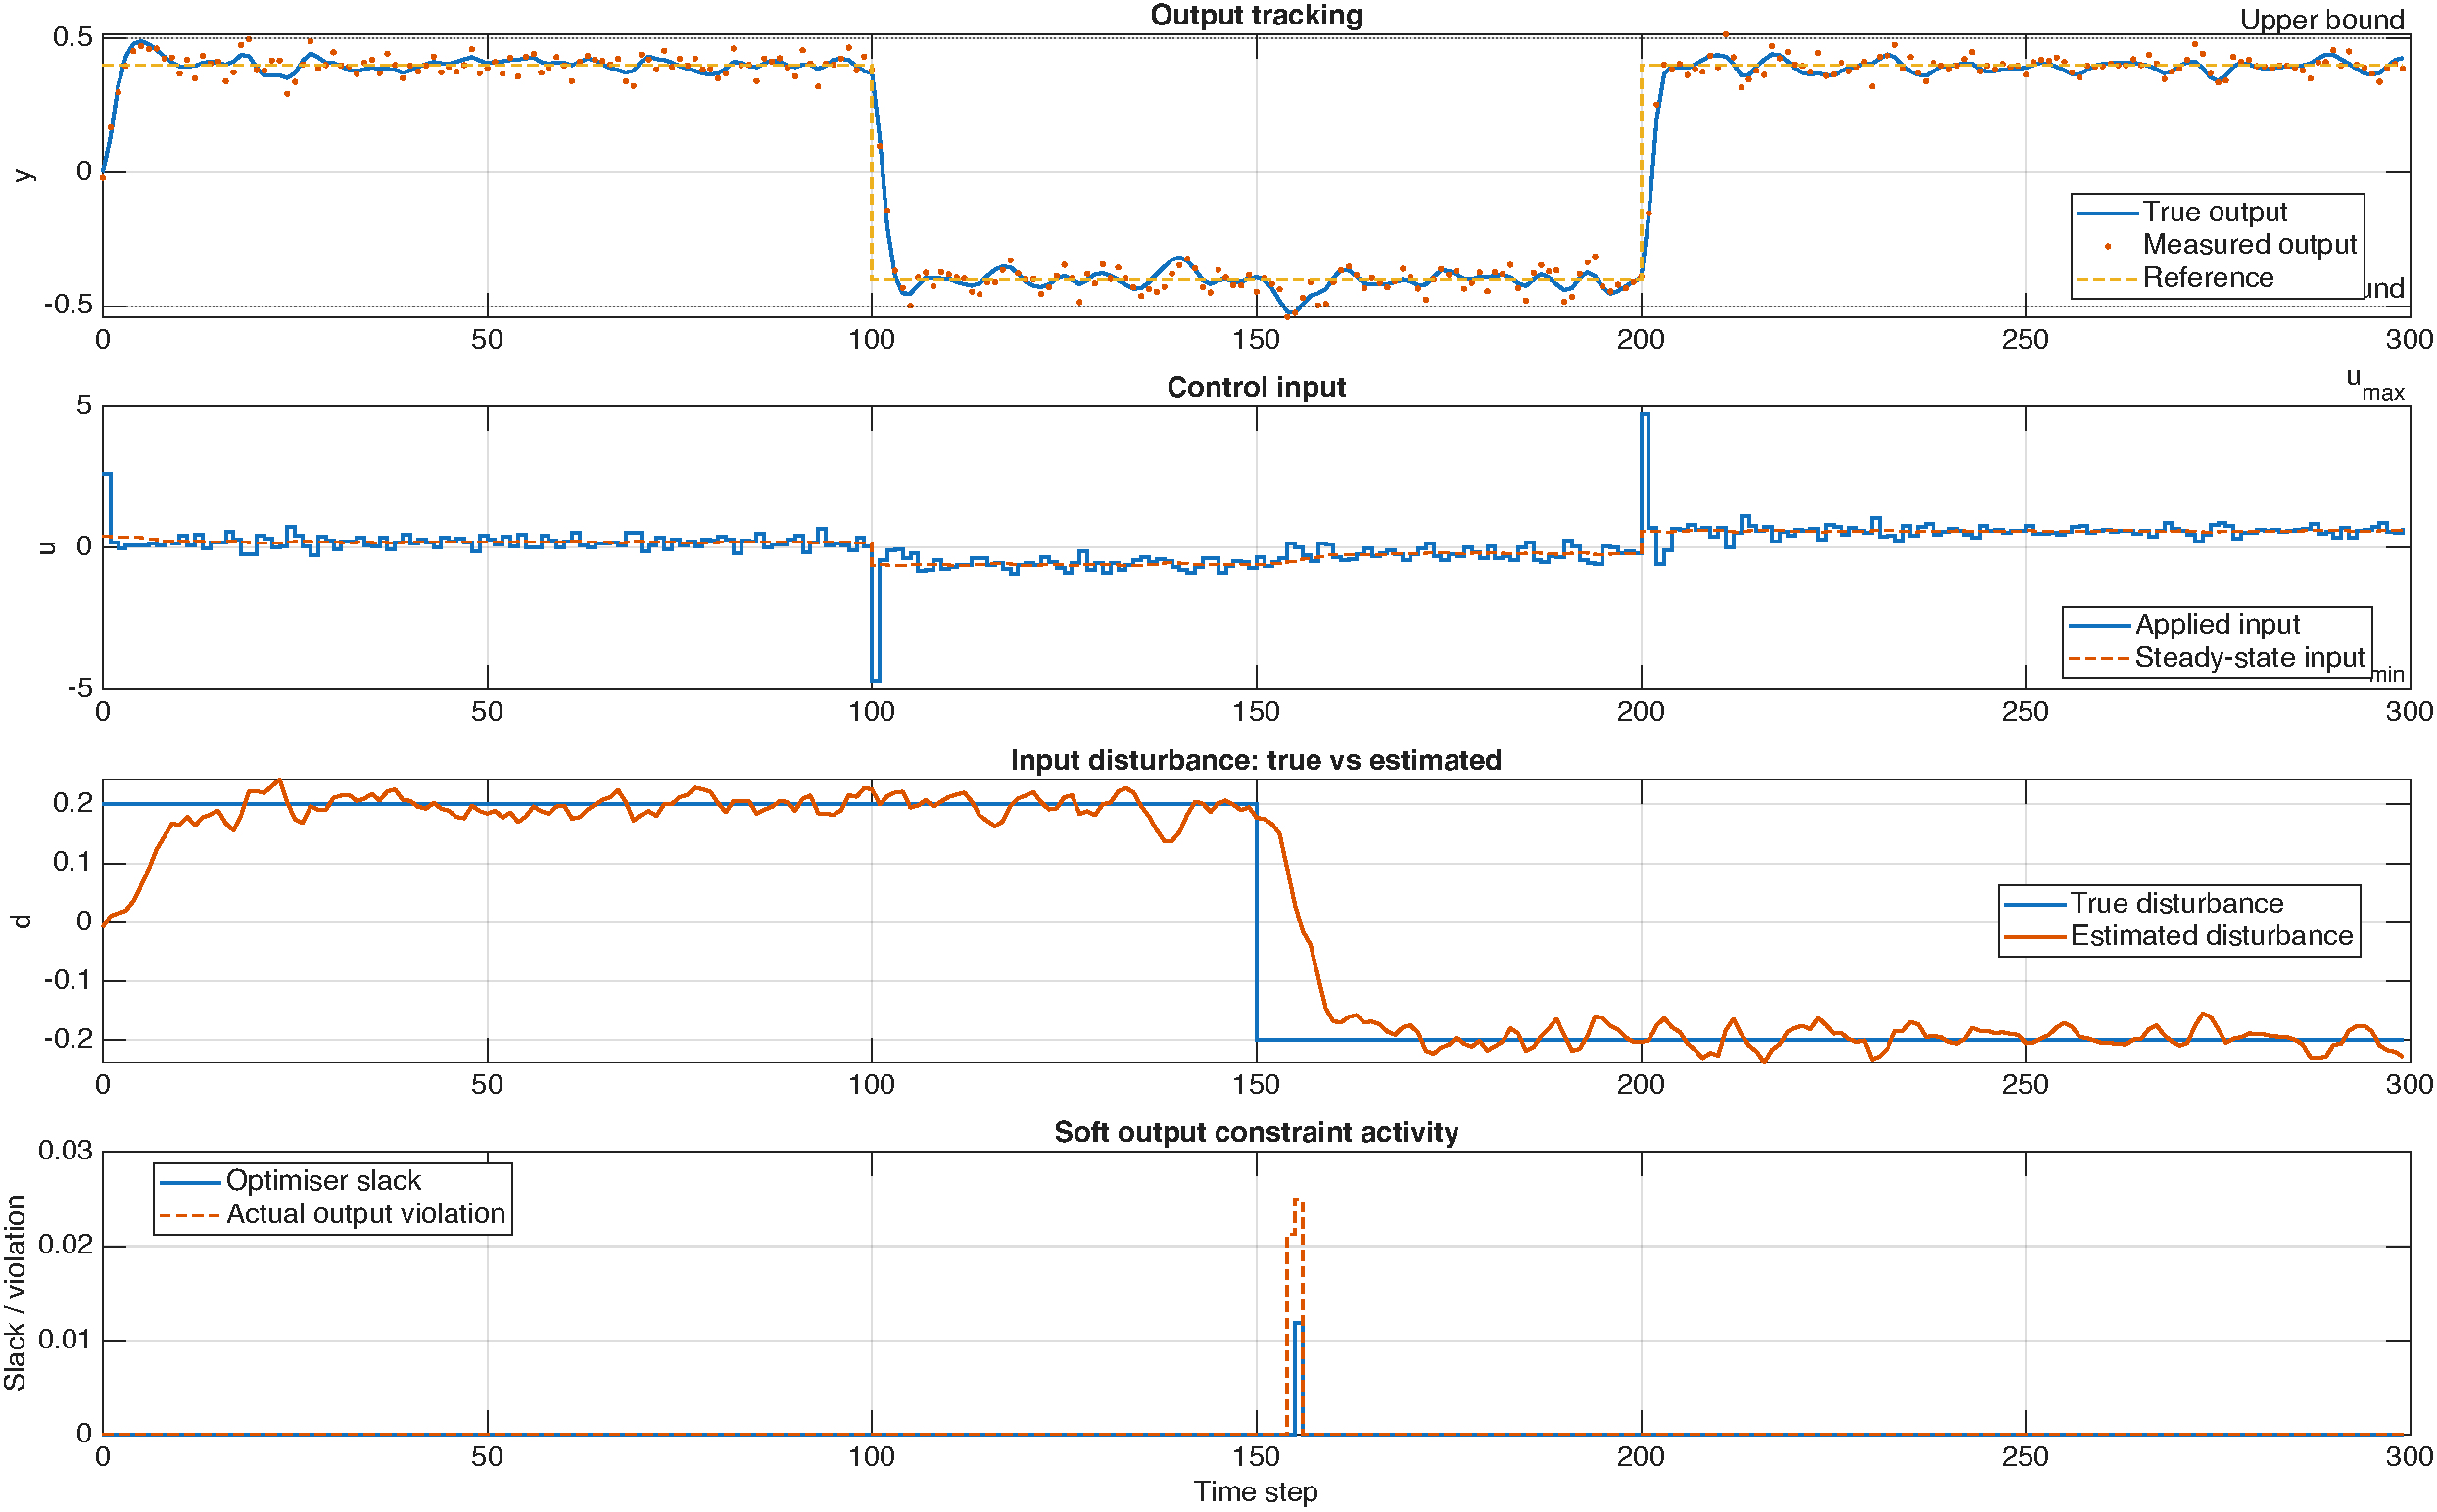
\includegraphics[width=1.0\linewidth]{Figures/Offsetfree_MPC.pdf}
	\caption{Closed-loop performance of the offset-free MPC with soft output constraints under piecewise-constant reference changes and an unknown step disturbance. The top panel shows accurate output tracking of the constrained reference whilst keeping the output close to the prescribed bounds. The second panel shows the applied control input together with the steady-state target input, with brief transient peaks at the reference-switching instants. The third panel shows that the augmented observer estimates the constant input disturbance well, including the disturbance sign change. The bottom panel shows that the soft output constraint is active only briefly during the disturbance transition, indicating that constraint violations are small and short-lived.}
	\label{fig:offset_free_results}
\end{figure}

The code follows the algorithm summarised in Algorithm~\ref{alg:offset_free_mpc}.

\begin{algorithm}
	\caption{Offset-Free MPC with Disturbance Estimation}
	\label{alg:offset_free_mpc}
	\begin{algorithmic}[1]
		\State \textbf{Input:} System matrices \((A,B,B_w,C)\), optional output-bias matrix \(C_d\), weights \((Q,R,P_{\mathrm{term}},\rho)\), input/output constraints, prediction horizon \(N\).
		\State \textbf{Output:} Control input \(u_k\).
		
		\Procedure{Offline Initialisation}{}
		\State Construct the augmented model
		\[
		z_k=
		\begin{bmatrix}
			x_k\\
			d_k
		\end{bmatrix},\qquad
		z_{k+1}=A_{\mathrm{aug}}z_k+B_{\mathrm{aug}}u_k,\qquad
		y_k=C_{\mathrm{aug}}z_k .
		\]
		\State Compute the estimator gain \(L\) from the DARE associated with \((A_{\mathrm{aug}},C_{\mathrm{aug}},W,V)\).
		\State Compute the terminal cost matrix \(P_{\mathrm{term}}\) for the deviation dynamics.
		\State Define the parametric MPC problem:
		\begin{align*}
			\min_{\tilde u,\epsilon}\quad
			&\sum_{i=0}^{N-1}
			\left(
			\|\tilde x_i\|_Q^2+\|\tilde u_i\|_R^2+\rho\|\epsilon_i\|^2
			\right)
			+\|\tilde x_N\|_{P_{\mathrm{term}}}^2 \\
			\text{s.t.}\quad
			&\tilde x_0=\hat x_k-x_{ss},\\
			&\tilde x_{i+1}=A\tilde x_i+B\tilde u_i,\qquad i=0,\dots,N-1,\\
			&u_{\min}\le \tilde u_i+u_{ss}\le u_{\max},\\
			&y_{\min,i}-\epsilon_i\le C(\tilde x_i+x_{ss})\le y_{\max,i}+\epsilon_i,\\
			&\epsilon_i\ge 0,\qquad i=0,\dots,N-1.
		\end{align*}
		\State Compile the solver object, including any real-time parameters required by the chosen formulation.
		\EndProcedure
		
		\Procedure{Online Control Loop}{}
		\State Initialise \(\hat z_{0|0}\), \(u_{-1}\), and optionally \(\hat d_{0}\).
		\For{$k=0,1,2,\dots$}
		\State Measure the output \(y_k\).
		
		\State \textit{// 1. Augmented-state estimation}
		\State \(\hat z_{k|k-1}\gets A_{\mathrm{aug}}\hat z_{k-1|k-1}+B_{\mathrm{aug}}u_{k-1}\)
		\State \(\hat z_{k|k}\gets \hat z_{k|k-1}+L\bigl(y_k-C_{\mathrm{aug}}\hat z_{k|k-1}\bigr)\)
		\State Extract \(\hat x_k\) and the raw disturbance estimate \(\hat d_{,k}\) from \(\hat z_{k|k}\).
	
		
		\State \textit{// 2. Steady-state target calculation}
		\State Compute \((x_{ss},u_{ss})\) from the current reference and disturbance estimate, either
		\[
		x_{ss}=Ax_{ss}+Bu_{ss}+B_w\hat d_k,\qquad
		r_k=Cx_{ss}+C_d\hat d_k,
		\]
		or, more generally, by solving a constrained steady-state optimisation problem.
		
		\State \textit{// 3. MPC regulation}
		\State Solve the MPC problem using the current parameters \((\hat x_k,x_{ss},u_{ss})\) and any future bound sequences if required.
		\State Obtain the first optimal move \(\tilde u_0^\star\).
		
		\State \textit{// 4. Apply input}
		\State \(u_k \gets \tilde u_0^\star + u_{ss}\)
		\State \(u_k \gets \max(u_{\min},\min(u_{\max},u_k))\)
		\State Apply \(u_k\) to the plant.
		\EndFor
		\EndProcedure
	\end{algorithmic}
\end{algorithm}

\noindent\textbf{Note.}
Algorithm~\ref{alg:offset_free_mpc} describes the general offset-free MPC structure based on augmented-state disturbance estimation, steady-state target calculation and deviation-form regulation. In the simplest reference-tracking case, the steady-state pair \((x_{ss},u_{ss})\) may be obtained directly from the linear equilibrium equations \eqref{eq:target_calc}. In constrained or economic MPC, however, it is generally more appropriate to compute \((x_{ss},u_{ss})\) by solving a constrained steady-state optimisation problem. Moreover, if soft output constraints are used, the slack variables must satisfy \(\epsilon_i \ge 0\), and the indexing of predicted outputs in the constraints should be chosen consistently with the state-update convention adopted in the MPC formulation.

\begin{examplebox}{MATLAB: Offset-Free MPC for Quadrotor Position Control}
	
	\textbf{1. Problem Formulation: Nonlinear Dynamics}
	
	We consider the translational dynamics of a quadrotor. Let \(p = [x, y, z]^T\) denote the position and \(v = [\dot{x}, \dot{y}, \dot{z}]^T\) the velocity. The control inputs are the roll angle \(\phi\), pitch angle \(\theta\), and total thrust \(T\). Assuming zero yaw \(\psi=0\), the translational equations of motion are
	\begin{align}
		\ddot{x} &= \frac{T}{m}\cos\phi \sin\theta + w_x \nonumber\\
		\ddot{y} &= -\frac{T}{m}\sin\phi + w_y \nonumber\\
		\ddot{z} &= \frac{T}{m}\cos\phi \cos\theta - g + w_z
		\label{eq:nonlinear_quad}
	\end{align}
	where \(m\) is the mass, \(g\) is gravity, and \(w=[w_x,w_y,w_z]^T\) represents external wind disturbances. These dynamics are nonlinear and coupled. Tilting to generate lateral motion, for example, reduces the vertical lift component and therefore changes the thrust required to maintain altitude.
	
	\textbf{2. Linearisation and Virtual Inputs}
	
	To design a linear MPC, we linearise the dynamics about the hover equilibrium. In hover, the attitude angles are small and the thrust balances gravity. Using the small-angle approximations \(\sin\theta \approx \theta\), \(\sin\phi \approx \phi\), \(\cos\phi \approx \cos\theta \approx 1\), \eqref{eq:nonlinear_quad} becomes
	\[
	\ddot{x} \approx g\theta, \qquad
	\ddot{y} \approx -g\phi, \qquad
	\ddot{z} \approx \frac{T}{m} - g.
	\]
	
	We now define the \textbf{virtual control inputs}
	\[
	u_{\mathrm{lin}} = [a_x,\ a_y,\ a_z]^T,
	\]
	which represent commanded translational accelerations. The corresponding mapping to physical inputs is
	\begin{equation} \label{eq:virtual_mapping}
		\begin{aligned}
			a_x &\triangleq g\theta & \Rightarrow \theta_{\mathrm{cmd}} &= \frac{a_x}{g},\\
			a_y &\triangleq -g\phi & \Rightarrow \phi_{\mathrm{cmd}} &= -\frac{a_y}{g},\\
			a_z &\triangleq \frac{T}{m} - g & \Rightarrow T_{\mathrm{cmd}} &= m(a_z + g).
		\end{aligned}
	\end{equation}
	
		\begin{center}
		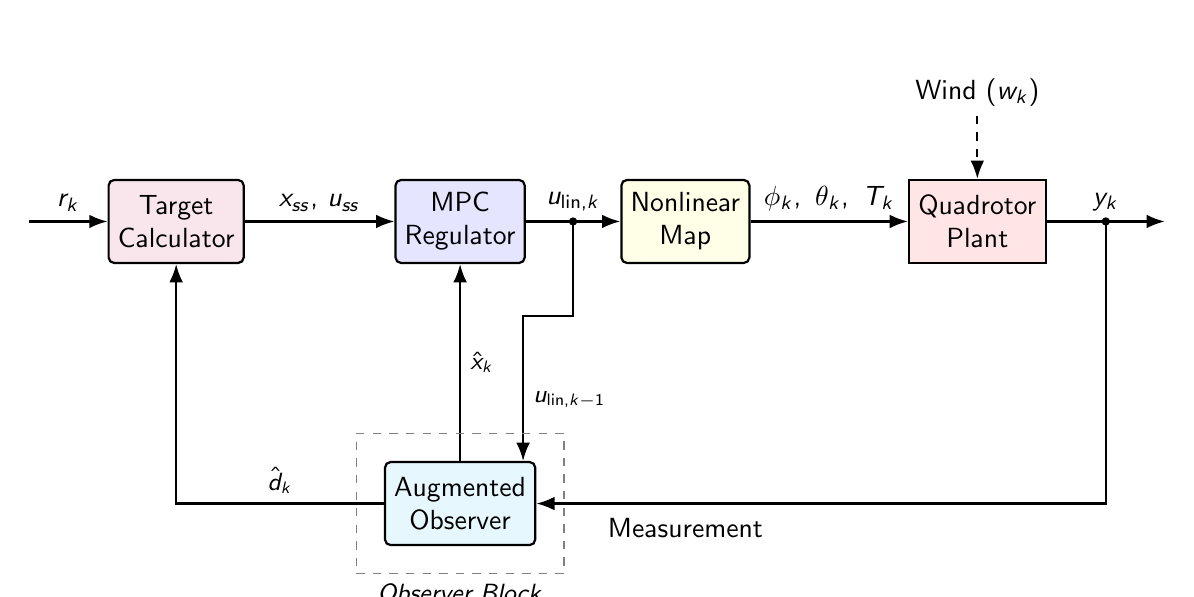
\begin{tikzpicture}[
			node distance = 1.8cm,
			auto,
			>=Latex,
			block/.style = {draw, rectangle, thick, minimum height=3em, minimum width=3.5em, align=center, fill=blue!5, rounded corners=2pt},
			plant/.style = {draw, rectangle, thick, minimum height=3em, minimum width=3.5em, fill=red!10, align=center},
			input/.style  = {coordinate},
			output/.style = {coordinate}
			]
			
			\node [input] (input) {};
			\node [block, right=1cm of input,  fill=purple!10] (target) {Target\\Calculator};
			\node [block, right=1.9cm of target, fill=blue!10] (mpc)    {MPC\\Regulator};
			\node [block, right=1.2cm of mpc,  fill=yellow!10] (map)    {Nonlinear\\Map};
			\node [plant, right=2cm of map]                    (plant)  {Quadrotor\\Plant};
			\node [output, right=1.5cm of plant]               (output) {};
			
			% Augmented Observer (no LPF sibling)
			\node [block, below=2.5cm of mpc, fill=cyan!10] (kf) {Augmented\\Observer};
			
			%% ── Forward path ──────────────────────────────────────────────
			\draw [->, thick] (input)  -- node[name=ref] {$r_k$}                     (target);
			\draw [->, thick] (target) -- node[above]    {$x_{ss},\,u_{ss}$}          (mpc);
			\draw [->, thick] (mpc)    -- node[above, name=ulin] {$u_{\mathrm{lin},k}$} (map);
			\draw [->, thick] (map)    -- node[above]    {$\phi_k,\ \theta_k,\ T_k$}  (plant);
			\draw [->, thick] (plant)  -- node[name=y] (y_node) {$y_k$}               (output);
			
			% Wind disturbance
			\node [above=0.8cm of plant] (wind) {Wind $(w_k)$};
			\draw [->, thick, dashed] (wind) -- (plant);
			
			%% ── Measurement feedback ──────────────────────────────────────
			\draw [->, thick] (y_node.south) |- (kf.east);
			\fill (y_node.south) circle (1.5pt);
			\node [below=3.1cm of map] {Measurement};
			
			%% ── Observer outputs ──────────────────────────────────────────
			% \hat x_k  ->  MPC
			\draw [->, thick] (kf.north) -- node[right, font=\small] {$\hat{x}_k$}
			($(mpc.south) + (0,0)$);
			
			% \hat d_k  ->  Target Calculator (single corner: left then up)
			\draw [->, thick] (kf.west) -|
			node[pos=0.25, above, font=\small] {$\hat{d}_k$}
			(target.south);
			
			%% ── Control input fed back to observer ────────────────────────
			\draw [->, thick] (ulin.south) -- ++(0,-1.2)
			-| node[pos=0.79, right, font=\small] {$u_{\mathrm{lin},k-1}$}
			($(kf.north) + (0.8,0)$);
			\fill (ulin.south) circle (1.5pt);
			
			%% ── Observer bounding box (kf only) ──────────────────────────
			\node [draw=gray, dashed, inner sep=10pt, fit=(kf),
			label=below:\small\textit{Observer Block}] (obs_box) {};
			
		\end{tikzpicture}
		
		\captionof{figure}{Control architecture for the quadrotor example. The target calculator uses the filtered wind estimate \(\hat d_k\) to compute steady-state targets \((x_{ss},u_{ss})\) in the linearised model. The MPC regulator computes the virtual input \(u_{\mathrm{lin},k}\), which is then mapped to the physical commands \((\phi_k,\theta_k,T_k)\). The observer uses the measured output and the previously applied virtual input.}
		\label{fig:quadrotor_control_architecture}
	\end{center}

	Substituting these virtual inputs into the linearised model decouples the motion into three double integrators, so that the discrete-time predictor used by the MPC has the form
	\[
	x_{k+1} = A x_k + B u_{\mathrm{lin},k}.
	\]
	
	\textbf{3. Offset-Free Control Strategy}
	
	The control loop proceeds in three stages:
	\begin{enumerate}
		\item \textbf{Estimation:} An augmented Kalman filter estimates the state and a constant disturbance vector representing wind acceleration. The raw disturbance estimate is then low-pass filtered to reduce noise.
		
		\item \textbf{Target Calculation:} Given the filtered disturbance estimate \(\hat d_k\), the steady-state pair \((x_{ss},u_{ss})\) is computed from the equilibrium equations
		\[
		\begin{bmatrix}
			I-A & -B\\
			C & 0
		\end{bmatrix}
		\begin{bmatrix}
			x_{ss}\\
			u_{ss}
		\end{bmatrix}
		=
		\begin{bmatrix}
			B_w \hat d_k\\
			r_{\mathrm{ref}}
		\end{bmatrix}.
		\]
		Here \(u_{ss}\) is the steady virtual acceleration required to counteract the estimated wind.
		
		\item \textbf{Regulation:} The MPC operates in deviation coordinates and computes the optimal corrective input sequence that steers the current state estimate towards the target.
	\end{enumerate}
	
	Finally, the virtual control input is mapped back to the physical commands \((\phi,\theta,T)\) using \eqref{eq:virtual_mapping}.
	
	\textbf{4. MATLAB Implementation}
	
	The code below simulates this strategy. The controller uses a linear prediction model, but the plant is simulated with the full nonlinear dynamics using RK4 integration. A step wind disturbance is applied at \(t=50\) s. Figure~\ref{fig:quad_mpc_result} shows the simulation result for tracking and disturbance observation. 
	
		\centering
		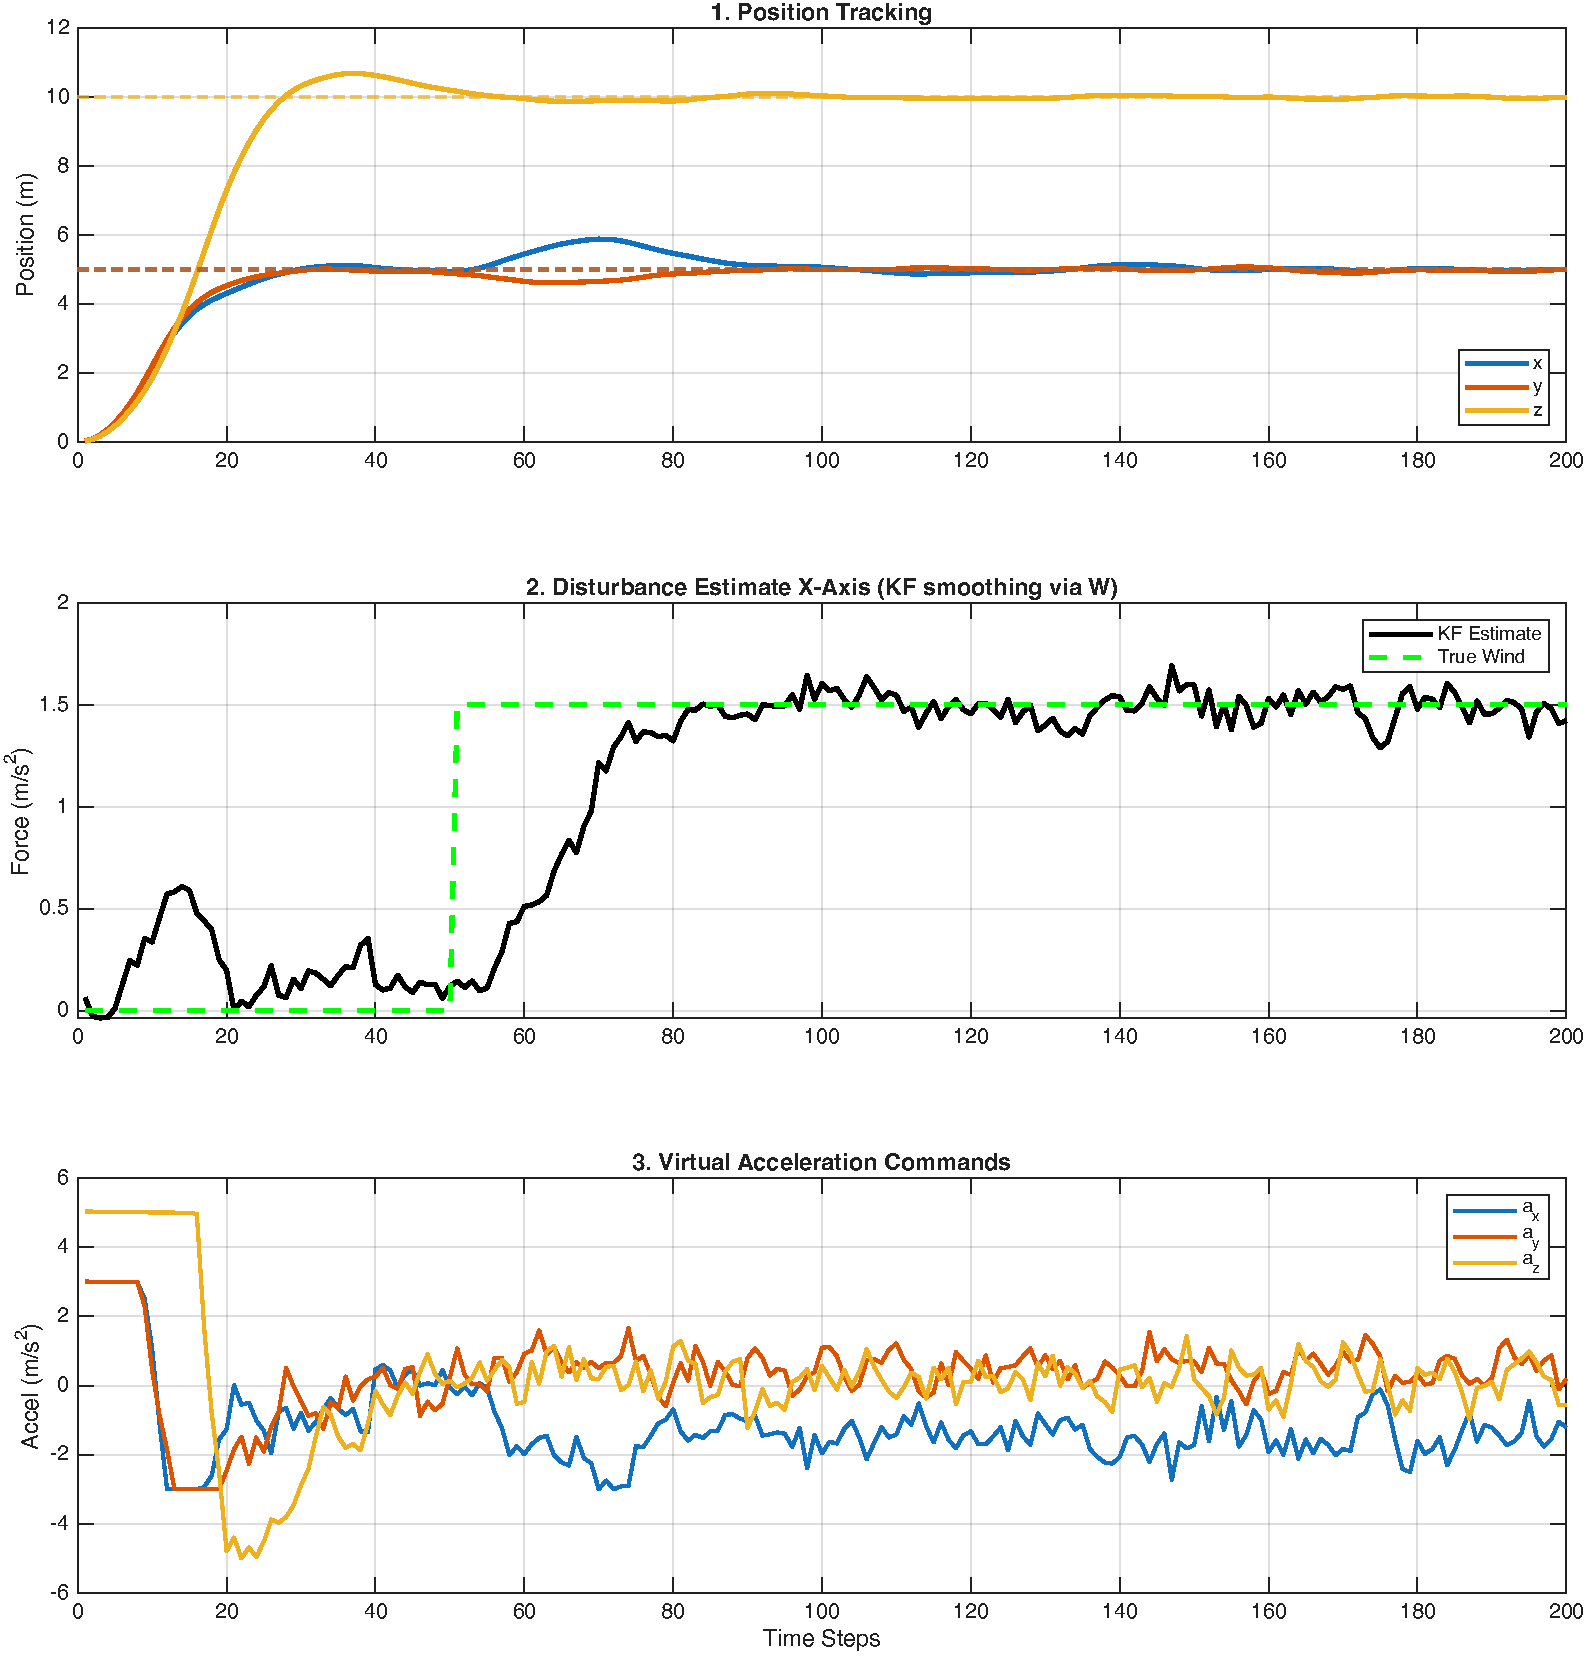
\includegraphics[width=0.9\linewidth]{Figures/Quadrotor_MPC.pdf}
		\captionof{figure}{\textbf{Simulation results: offset-free MPC on a nonlinear quadrotor.} \textbf{Top:} Position tracking. The quadrotor tracks the reference setpoint \([5,5,10]\) m. At \(t=50\) s, a step wind disturbance is applied in the horizontal plane; the trajectory deviates transiently and then returns to the reference with negligible steady-state error. \textbf{Middle:} Disturbance estimation using Kalman Filter. The  estimate converges towards the true wind disturbance. \textbf{Bottom:} Virtual control inputs. After the wind disturbance is applied, the controller settles to non-zero steady virtual accelerations that counteract the wind and maintain the reference position.}
		\label{fig:quad_mpc_result}

	
	\begin{lstlisting}[language=Matlab]
clear; clc; close all;

%% 1. System & Linear Model
g = 9.81; m = 1.0; dt = 0.1;
Ac = [zeros(3,3) eye(3); zeros(3,3) zeros(3,3)];
Bc = [zeros(3,3); eye(3)];
Cc = [eye(3), zeros(3,3)];
sys_d = c2d(ss(Ac, Bc, Cc, 0), dt, 'zoh');
A = sys_d.A; B = sys_d.B; C = sys_d.C;
nx = 6; nu = 3; ny = 3;

%% 2. Augmented Observer
Bw = B;
A_aug = [A, Bw; zeros(3,nx), eye(3)];
B_aug = [B; zeros(3,nu)];
C_aug = [C, zeros(3,3)];

% --- KEY TUNING ---
% W(1:6,1:6)  : process noise on physical states  (keep small)
% W(7:9,7:9)  : process noise on disturbance states
%   LOWER  -> Kalman gain for d is small -> slow update -> implicit LPF
%   HIGHER -> fast disturbance tracking  -> noisier estimate
W = diag([1e-3*ones(1,6), 5e-3*ones(1,3)]);   
V = 1e-2 * eye(3);                              

[P_obs,~,~] = dare(A_aug', C_aug', W, V);
L = P_obs * C_aug' / (C_aug * P_obs * C_aug' + V);

%% 3. Target Calculator
M_target = [eye(nx)-A, -B; C, zeros(ny,nu)];
P_target = pinv(M_target);

%% 4. MPC Formulation (Deviation Form)
N = 50;
Q = diag([20 20 40, 1 1 1]);
R = diag([2 2 2]);
rho = 1e4;
[P_term,~,~] = dare(A, B, Q, R);

du    = sdpvar(nu, N, 'full');
dx    = sdpvar(nx, N+1, 'full');
slack = sdpvar(nu, N, 'full');
x_hat = sdpvar(nx, 1);
x_ss  = sdpvar(nx, 1);
u_ss  = sdpvar(nu, 1);

obj  = 0;
cons = [dx(:,1) == x_hat - x_ss];
for k = 1:N
	cons = [cons, dx(:,k+1) == A*dx(:,k) + B*du(:,k)];
	obj  = obj + dx(:,k)'*Q*dx(:,k) + du(:,k)'*R*du(:,k) + rho*norm(slack(:,k),2)^2;
	u_abs = du(:,k) + u_ss;
	cons = [cons, -3 - slack(1:2,k) <= u_abs(1:2) <= 3 + slack(1:2,k)];
	cons = [cons, -5 - slack(3,k)   <= u_abs(3)   <= 5 + slack(3,k)];
	cons = [cons, slack(:,k) >= 0];
end
obj = obj + dx(:,N+1)'*P_term*dx(:,N+1);
ops = sdpsettings('solver','quadprog','verbose',0);
controller = optimizer(cons, obj, ops, {x_hat, x_ss, u_ss}, du(:,1));

%% 5. Simulation Loop
T_sim      = 200;
x_true     = zeros(6,1);
u_applied  = zeros(3,1);
z_est      = zeros(9,1);
wind_force = [0;0;0];
ref        = [5; 5; 10];

log_x      = zeros(3, T_sim);
log_u      = zeros(3, T_sim);
log_d      = zeros(3, T_sim);
log_d_true = zeros(3, T_sim);

for t = 1:T_sim
	if t > 50, 
		wind_force = [1.5; -0.5; 0]; 
	end

	% A. Measure & Estimate
	y_meas = C*x_true + sqrt(0.01)*randn(3,1);
	z_pred = A_aug*z_est + B_aug*u_applied;
	y_pred = C_aug*z_pred;
	z_est  = z_pred + L*(y_meas - y_pred);
	
	x_hat_val = z_est(1:6);
	d_hat     = z_est(7:9);   
	
	% B. Calculate Targets
	rhs      = [Bw * d_hat; ref];
	ss_sol   = P_target * rhs;
	x_target = ss_sol(1:nx);
	u_target = ss_sol(nx+1:end);
	
	% C. MPC Solve
	[du_opt, err] = controller{x_hat_val, x_target, u_target};
	if err, 
		du_opt = zeros(3,1); 
	end
	u_mpc = du_opt + u_target;
	
	% D. Nonlinear Mapping & Saturation
	accel_z_total = u_mpc(3) + g;
	Thrust    = m * accel_z_total;
	theta_cmd = max(-0.5, min(0.5,  u_mpc(1) / g));
	phi_cmd   = max(-0.5, min(0.5, -u_mpc(2) / g));
	Thrust    = max(0,    min(20,   Thrust));
	u_phys    = [phi_cmd; theta_cmd; Thrust];
	
	% E. Plant Update (Nonlinear)
	x_true    = rk4_step(@quadrotor_dyn, x_true, u_phys, wind_force, dt, m, g);
	u_applied = u_mpc;
	
	log_x(:,t)      = x_true(1:3);
	log_u(:,t)      = u_mpc;
	log_d(:,t)      = d_hat;
	log_d_true(:,t) = wind_force;
end

%% Plotting
t_vec = 1:T_sim;
figure('Color','w','Position',[100 100 800 800]);

subplot(3,1,1);
h = plot(t_vec, log_x, 'LineWidth', 2); hold on;
clr = get(gca,'ColorOrder');
yline(ref(1),'--','Color',clr(1,:),'LineWidth',1.5);
yline(ref(2),'--','Color',clr(2,:),'LineWidth',1.5);
yline(ref(3),'--','Color',clr(3,:),'LineWidth',1.5);
grid on; ylabel('Position (m)');
title('1. Position Tracking');
legend(h,{'x','y','z'},'Location','SouthEast');

subplot(3,1,2);
plot(t_vec, log_d(1,:),      'k',  'LineWidth', 2); hold on;
plot(t_vec, log_d_true(1,:), 'g--','LineWidth', 2);
grid on; ylabel('Force (m/s^2)');
title('2. Disturbance Estimate X-Axis (KF smoothing via W)');
legend('KF Estimate','True Wind');

subplot(3,1,3);
plot(t_vec, log_u, 'LineWidth', 1.5);
legend('a_x','a_y','a_z');
grid on; title('3. Virtual Acceleration Commands');
ylabel('Accel (m/s^2)'); xlabel('Time Steps');

%% Helper Functions
function x_next = rk4_step(fun, x, u, w, dt, m, g)
	k1 = fun(x,           u, w, m, g);
	k2 = fun(x+0.5*dt*k1, u, w, m, g);
	k3 = fun(x+0.5*dt*k2, u, w, m, g);
	k4 = fun(x+dt*k3,     u, w, m, g);
	x_next = x + (dt/6)*(k1 + 2*k2 + 2*k3 + k4);
end

function dxdt = quadrotor_dyn(x, u, w, m, g)
	phi = u(1); theta = u(2); T = u(3);
	Fx  = T*(cos(phi)*sin(theta));
	Fy  = T*(-sin(phi));
	Fz  = T*(cos(phi)*cos(theta));
	ax  = (Fx + w(1))/m;
	ay  = (Fy + w(2))/m;
	az  = (Fz + w(3))/m - g;
	dxdt = [x(4:6); ax; ay; az];
end

	\end{lstlisting}
\end{examplebox}





\begin{examplebox}{Single-zone building heating with economic offset-free MPC}
We consider a heated office room ($\sim$50~m$^2$) whose thermal dynamics
are described by a three-state physically derived RC model discretised at
$T_s = 1800\,\text{s}$ (30~min) via the matrix exponential.
The states are
\[
x_k = \begin{bmatrix} T_{\mathrm{air},k} \\ T_{w,\mathrm{in},k} \\ T_{w,\mathrm{out},k} \end{bmatrix}\!,
\]
representing indoor air temperature, inner wall layer temperature, and
outer wall layer temperature (all in $^\circ$C).
The discrete-time model is
\[
x_{k+1} = A x_k + B u_k + E\,T_{\mathrm{amb},k}
+ B_{\mathrm{sol}}\,\varphi_{\mathrm{sol},k}
+ B_w\,d_k,
\qquad
y_k = C x_k,
\]
where $u_k \in [0, 2000]$~W is the heater power,
$T_{\mathrm{amb},k}$ ($^\circ$C) is the \emph{measured} outdoor temperature,
$\varphi_{\mathrm{sol},k}$ (W/m$^2$) is the \emph{measured} solar
irradiance (both treated as known feedforwards), and $d_k$
($^\circ$C/step) is an \emph{unmeasured} scaled disturbance representing
occupancy and internal heat gains. The output
$y_k = 0.56\,T_{\mathrm{air},k} + 0.44\,T_{w,\mathrm{in},k}$
is the operative temperature (ISO~7726), measured with noise standard
deviation $\sigma_v = 0.1\,^\circ$C.

The pre-computed discrete model matrices are
\begin{align*}
	A &= \begin{bmatrix} 0.8753 & 0.1102 & 0.0004 \\ 0.0275 & 0.9649 & 0.0073 \\ 0.0001 & 0.0049 & 0.9851 \end{bmatrix}, \\[6pt]
	B &= \begin{bmatrix} 7.91\times10^{-4} \\ 1.00\times10^{-4} \\ 0 \end{bmatrix}\!, \quad
	E  = \begin{bmatrix} 0.01404 \\ 0.00025 \\ 0.00993 \end{bmatrix}\!, \quad
	B_{\mathrm{sol}} = \begin{bmatrix} 9.04\times10^{-6} \\ 1.43\times10^{-6} \\ 3.47\times10^{-4} \end{bmatrix}\!, \\[6pt]
	B_w &= \begin{bmatrix} 1.7647 \\ 0.0267 \\ 0 \end{bmatrix}\!, \quad
	C  = \begin{bmatrix} 0.56 & 0.44 & 0 \end{bmatrix}.
\end{align*}

\medskip
\textbf{Exogenous profiles (48-hour winter scenario):}
\begin{itemize}
	\item \textbf{Outdoor temperature} $(T_{\mathrm{amb},k})$:
	\[
	T_{\mathrm{amb},k} = 5 + 6\sin\!\left(\tfrac{2\pi(t_k-14)}{24}\right) + 0.5\,\eta_k,
	\]
	ranging nominally between $-1\,^\circ$C and $11\,^\circ$C; treated as
	a known feedforward.
	
	\item \textbf{Solar irradiance} $(\varphi_{\mathrm{sol},k})$:
	\[
	\varphi_{\mathrm{sol},k} = \max\!\left(0,\; 600\sin\!\left(\tfrac{\pi(\mathrm{mod}(t_k,24)-8)}{9}\right)\right),
	\]
	treated as a known feedforward.
	
	\item \textbf{Occupancy disturbance} $(d_k)$: an effective scaled thermal
	disturbance,
	\[
	d_k = \begin{cases} 0.191\,^\circ\text{C/step} & 08{:}00 \le \mathrm{time}(t_k) < 18{:}00, \\ 0 & \text{otherwise,} \end{cases}
	\]
	corresponding to 300~W of internal gains; \emph{unknown} to the
	controller and estimated by the Kalman filter.
	
	\item \textbf{Electricity price} $(p_k)$:
	\[
	p_k = \begin{cases} 0.28\,\pounds/\text{kWh} & 07{:}00 \le \mathrm{time}(t_k) < 22{:}00, \\ 0.05\,\pounds/\text{kWh} & \text{otherwise.} \end{cases}
	\]
\end{itemize}

\textbf{Time-varying comfort bounds:}
\[
[y_{\min,k},\,y_{\max,k}] = \begin{cases} [20,\,23]\,^\circ\text{C} & \text{daytime }(07{:}00\text{--}22{:}00), \\ [15,\,26]\,^\circ\text{C} & \text{night-time.}\end{cases}
\]

\medskip
\textbf{Control architecture (three layers):}

\begin{enumerate}
	
	\item \textbf{Augmented Kalman observer.}
	The disturbance is appended to the state as a random walk,
	$z_k = [x_k^\top,\, d_k]^\top$, giving the augmented model
	\[
	z_{k+1} =
	\begin{bmatrix} A & B_w \\ 0 & 1 \end{bmatrix} z_k
	+ \begin{bmatrix} B \\ 0 \end{bmatrix} u_k
	+ \begin{bmatrix} E \\ 0 \end{bmatrix} T_{\mathrm{amb},k}
	+ \begin{bmatrix} B_{\mathrm{sol}} \\ 0 \end{bmatrix} \varphi_{\mathrm{sol},k},
	\]
	\[
	y_k = [C,\;0]\,z_k + v_k.
	\]
	 The process noise covariance is selected as
	$W = \mathrm{diag}(10^{-3},10^{-3},10^{-3},\,(0.01)^2)$
	is directly interpretable: $\sqrt{W_d}=0.01\,^\circ$C/step
	represents the expected occupancy change between sampling instants.
	The steady-state Kalman gain $L$ is obtained from the DARE with
	measurement noise variance $V=0.01$.
	
	\item \textbf{Economic steady-state target calculator.}
	At each step, the following QP selects an economically optimal
	steady-state pair $(x_{ss}, u_{ss})$:
	\begin{align*}
		\min_{x_{ss},u_{ss},\epsilon_{ss}} \quad
		& p_k\,u_{ss} + 10^4\,\epsilon_{ss}^2 \\
		\text{s.t.} \quad
		& x_{ss} = A x_{ss} + B u_{ss}
		+ E T_{\mathrm{amb},k}
		+ B_{\mathrm{sol}}\varphi_{\mathrm{sol},k}
		+ B_w \hat d_k, \\
		& y_{\min,k}-\epsilon_{ss} \le C x_{ss} \le y_{\max,k}+\epsilon_{ss},
		\quad 0 \le u_{ss} \le 2000,\quad \epsilon_{ss}\ge 0.
	\end{align*}
	
	\item \textbf{Economic MPC regulator with price preview.}
	Defining $\tilde x_i = x_i - x_{ss}$, $\tilde u_i = u_i - u_{ss}$,
	the regulator solves over a horizon $N=24$ (12~hours):
	\begin{align*}
		\min_{\tilde u,\epsilon} \quad &
		\sum_{i=0}^{N-1}\!\Bigl(
		\|\tilde x_{i+1}\|_Q^2
		+\beta\,p_{k+i}\,(\tilde u_i+u_{ss})\tfrac{T_s}{3600}
		+\rho\,\epsilon_i^2
		\Bigr) + \|\tilde x_N\|_P^2 \\
		\text{s.t.} \quad
		& \tilde x_0 = \hat x_k - x_{ss}, \\
		& \tilde x_{i+1} = A\tilde x_i + B\tilde u_i, \\
		& 0 \le \tilde u_i + u_{ss} \le 2000, \\
		& y_{\min,k+i}-\epsilon_i \le C(\tilde x_{i+1}+x_{ss}) \le y_{\max,k+i}+\epsilon_i,
		\quad \epsilon_i\ge 0,
	\end{align*}
	with $Q=\mathrm{diag}(5,2,1)$, $\beta=6$, $\rho=10^7$, and
	$P$ from the DARE.
	The term $\beta p_{k+i}(\tilde u_i+u_{ss})(T_s/3600)$ is the actual
	energy expenditure in pounds at future step $k+i$.
	The penalty hierarchy
	$\rho \gg \beta\,p_{\max}\,u_{\max}\,(T_s/3600)$,
	i.e.\ $10^7 \gg 1680$, ensures comfort violations are never
	preferred over heating.
\end{enumerate}

\textbf{MATLAB implementation:} The plotting section is omitted below.

\begin{lstlisting}[language=MATLAB]
	clear; clc; close all; rng(1);
	
	%% 1. Pre-computed Discrete Model (3R2C, ZOH, Ts = 1800 s)
	%    x = [T_air; T_w_in; T_w_out] (degC)
	%    u = heater power (W),  u in [0, 2000]

	Ts = 1800;
	A  = [	0.8753, 0.1102, 0.0004;
				0.0275, 0.9649, 0.0073;
				0.0001, 0.0049, 0.9851];
	B      = [7.91e-4; 1.00e-4; 0      ];
	E      = [0.01404; 0.00025; 0.00993];   
	Bsol   = [9.04e-6; 1.43e-6; 3.47e-4];  
	Bw     = [1.7647;  0.0267;  0      ];   
	C      = [0.56, 0.44, 0];               
	
	nx = 3;  nu = 1;  ny = 1; u_min = 0;  u_max = 2000;
	
	%% 2. Augmented Kalman Observer
	%    z = [x; d],  random-walk disturbance model
	
	A_aug = [A, Bw; zeros(1,nx), 1];
	B_aug = [B; 0];  E_aug = [E; 0];  Bsol_aug = [Bsol; 0];
	C_aug = [C, 0];
	
	W_kf = diag([1e-3, 1e-3, 1e-3, (0.01)^2]);  
	V_kf = 0.1^2;
	
	[P_kf,~,~] = dare(A_aug', C_aug', W_kf, V_kf);
	L_kf = P_kf*C_aug'/(C_aug*P_kf*C_aug' + V_kf);
	
	%% 3. Economic Steady-State Target Calculator
	price_in   = sdpvar(1);  d_in     = sdpvar(1);
	T_amb_in   = sdpvar(1);  phi_in   = sdpvar(1);
	y_min_in   = sdpvar(1);  y_max_in = sdpvar(1);
	xs = sdpvar(nx,1);  us = sdpvar(nu,1);  ss_slack = sdpvar(1);
	
	ss_cons = [xs == A*xs + B*us + E*T_amb_in + Bsol*phi_in + Bw*d_in, ...
	y_min_in - ss_slack <= C*xs <= y_max_in + ss_slack, ...
	u_min <= us <= u_max, ss_slack >= 0];
	ss_obj  = price_in*us + 1e4*ss_slack^2;
	
	target_calc = optimizer(ss_cons, ss_obj, ...
	sdpsettings('solver','quadprog','verbose',0), ...
	{price_in, d_in, T_amb_in, phi_in, y_min_in, y_max_in}, [xs; us]);
	
	%% 4. Economic MPC Regulator with Price Preview (N = 24, horizon = 12 h)
	%    Stage cost: ||x_tilde||_Q^2 + beta*price*u*(Ts/3600) + rho*slack^2
	%    Penalty hierarchy: rho >> beta*p_max*u_max*(Ts/3600)
	%    i.e.  1e7 >> 10*0.28*2000*0.5 = 2800
	N = 24;  Q = diag([5,2,1]);  rho = 1e7;  beta = 6;
	[P_term,~,~] = dare(A, B, Q, 1e-3);
	
	du        = sdpvar(nu,N,'full');   dx    = sdpvar(nx,N+1,'full');
	mpc_slack = sdpvar(1,N,'full');
	xhat_in   = sdpvar(nx,1);  xss_in = sdpvar(nx,1);  uss_in = sdpvar(nu,1);
	Ymin_seq  = sdpvar(1,N,'full');    Ymax_seq  = sdpvar(1,N,'full');
	Price_seq = sdpvar(1,N,'full');
	
	mpc_obj  = 0;
	mpc_cons = [dx(:,1) == xhat_in - xss_in];
	for i = 1:N
		u_abs    = du(:,i) + uss_in;
		x_pred_i = dx(:,i+1) + xss_in;
		mpc_cons = [mpc_cons, ...
		dx(:,i+1) == A*dx(:,i) + B*du(:,i), ...
		u_min <= u_abs <= u_max, ...
		Ymin_seq(i)-mpc_slack(i) <= C*x_pred_i <= Ymax_seq(i)+mpc_slack(i), ...
		mpc_slack(i) >= 0];
		mpc_obj = mpc_obj + dx(:,i)'*Q*dx(:,i) ...
		+ beta*Price_seq(i)*u_abs*(Ts/3600) ...
		+ rho*mpc_slack(i)^2;
	end
	mpc_obj = mpc_obj + dx(:,N+1)'*P_term*dx(:,N+1);
	
	mpc_reg = optimizer(mpc_cons, mpc_obj, ...
	sdpsettings('solver','quadprog','verbose',0), ...
	{xhat_in,xss_in,uss_in,Ymin_seq,Ymax_seq,Price_seq}, du(:,1));
	
	%% 5. Exogenous Profiles (48-hour simulation)
	N_sim   = 48*(3600/Ts);
	t_hours = (0:N_sim+N)*(Ts/3600);
	
	T_amb_profile = 5 + 6*sin(2*pi*(t_hours-14)/24) + 0.5*randn(size(t_hours));
	Solar_profile = max(0, 600*sin(pi*(mod(t_hours,24)-8)/9));
	Elec_Price    = 0.05*ones(size(t_hours));
	day_mask      = mod(t_hours,24) >= 7 & mod(t_hours,24) < 22;
	Elec_Price(day_mask) = 0.28;
	Tmin_profile  = 15*ones(size(t_hours));  Tmin_profile(day_mask) = 20;
	Tmax_profile  = 26*ones(size(t_hours));  Tmax_profile(day_mask) = 23;
	% True occupancy: 300 W = 0.191 degC/step (unknown to controller)
	d_occ_profile = 0.191*double(mod(t_hours,24) >= 8 & mod(t_hours,24) < 18);
	
	%% 6. Closed-Loop Simulation
	x_true = [19; 17; 10];  z_est = [19; 17; 10; 0];  u_prev = 0;
	
	log_Top  = zeros(1,N_sim);  log_Tmeas = zeros(1,N_sim);
	log_u    = zeros(1,N_sim);  log_d_est = zeros(1,N_sim);
	log_dtrue= zeros(1,N_sim);  log_price = zeros(1,N_sim);
	log_Tmin = zeros(1,N_sim);  log_Tmax  = zeros(1,N_sim);
	log_cost = zeros(1,N_sim);
	
	for k = 1:N_sim
		T_amb_k   = T_amb_profile(k);
		phi_sol_k = Solar_profile(k);
		y_meas    = C*x_true + sqrt(V_kf)*randn;
		
		% KF predict & correct (current-step feedforwards)
		if k == 1,  
			z_pred = z_est;
		else
			z_pred = A_aug*z_est + B_aug*u_prev ...
		+ E_aug*T_amb_k + Bsol_aug*phi_sol_k;
		end
		z_est = z_pred + L_kf*(y_meas - C_aug*z_pred);
		x_hat = z_est(1:nx);  d_hat = z_est(end);
		
		% Economic target
		y_min = Tmin_profile(k);  y_max = Tmax_profile(k);
		[ss_sol, err_ss] = target_calc{Elec_Price(k),d_hat,T_amb_k,phi_sol_k,y_min,y_max};
		if err_ss ~= 0,  
			x_ss = x_hat; 	u_ss = u_prev;
		else,  
			ss_sol=full(ss_sol); x_ss=ss_sol(1:nx); u_ss=ss_sol(nx+1);
		end
		% Economic MPC with N-step price preview
		[du_opt, err_mpc] = mpc_reg{x_hat, x_ss, u_ss, ...
				Tmin_profile(k+1:k+N), Tmax_profile(k+1:k+N), Elec_Price(k+1:k+N)};
		if err_mpc ~= 0,  
			du_opt = 0;  
		else,  
			du_opt = full(du_opt);  
		end
		u_prev = min(max(u_ss + du_opt, u_min), u_max);
	
		% Plant update (true occupancy unknown to controller)
		x_true = A*x_true + B*u_prev + E*T_amb_k ...
		+ Bsol*phi_sol_k + Bw*d_occ_profile(k);
		
		% Logging
		log_Top(k)  = C*x_true;   log_Tmeas(k) = y_meas;
		log_u(k)    = u_prev;      log_d_est(k) = d_hat;
		log_dtrue(k)= d_occ_profile(k);
		log_Tmin(k) = y_min;       log_Tmax(k)  = y_max;
		log_price(k)= Elec_Price(k);
		log_cost(k) = Elec_Price(k)*u_prev*(Ts/3600)/1000;  % GBP per step
	end
	fprintf('Total heating cost: GBP %.3f\n', sum(log_cost));
	
	% Visualisation is omitted for brevity
\end{lstlisting}

	\centering
	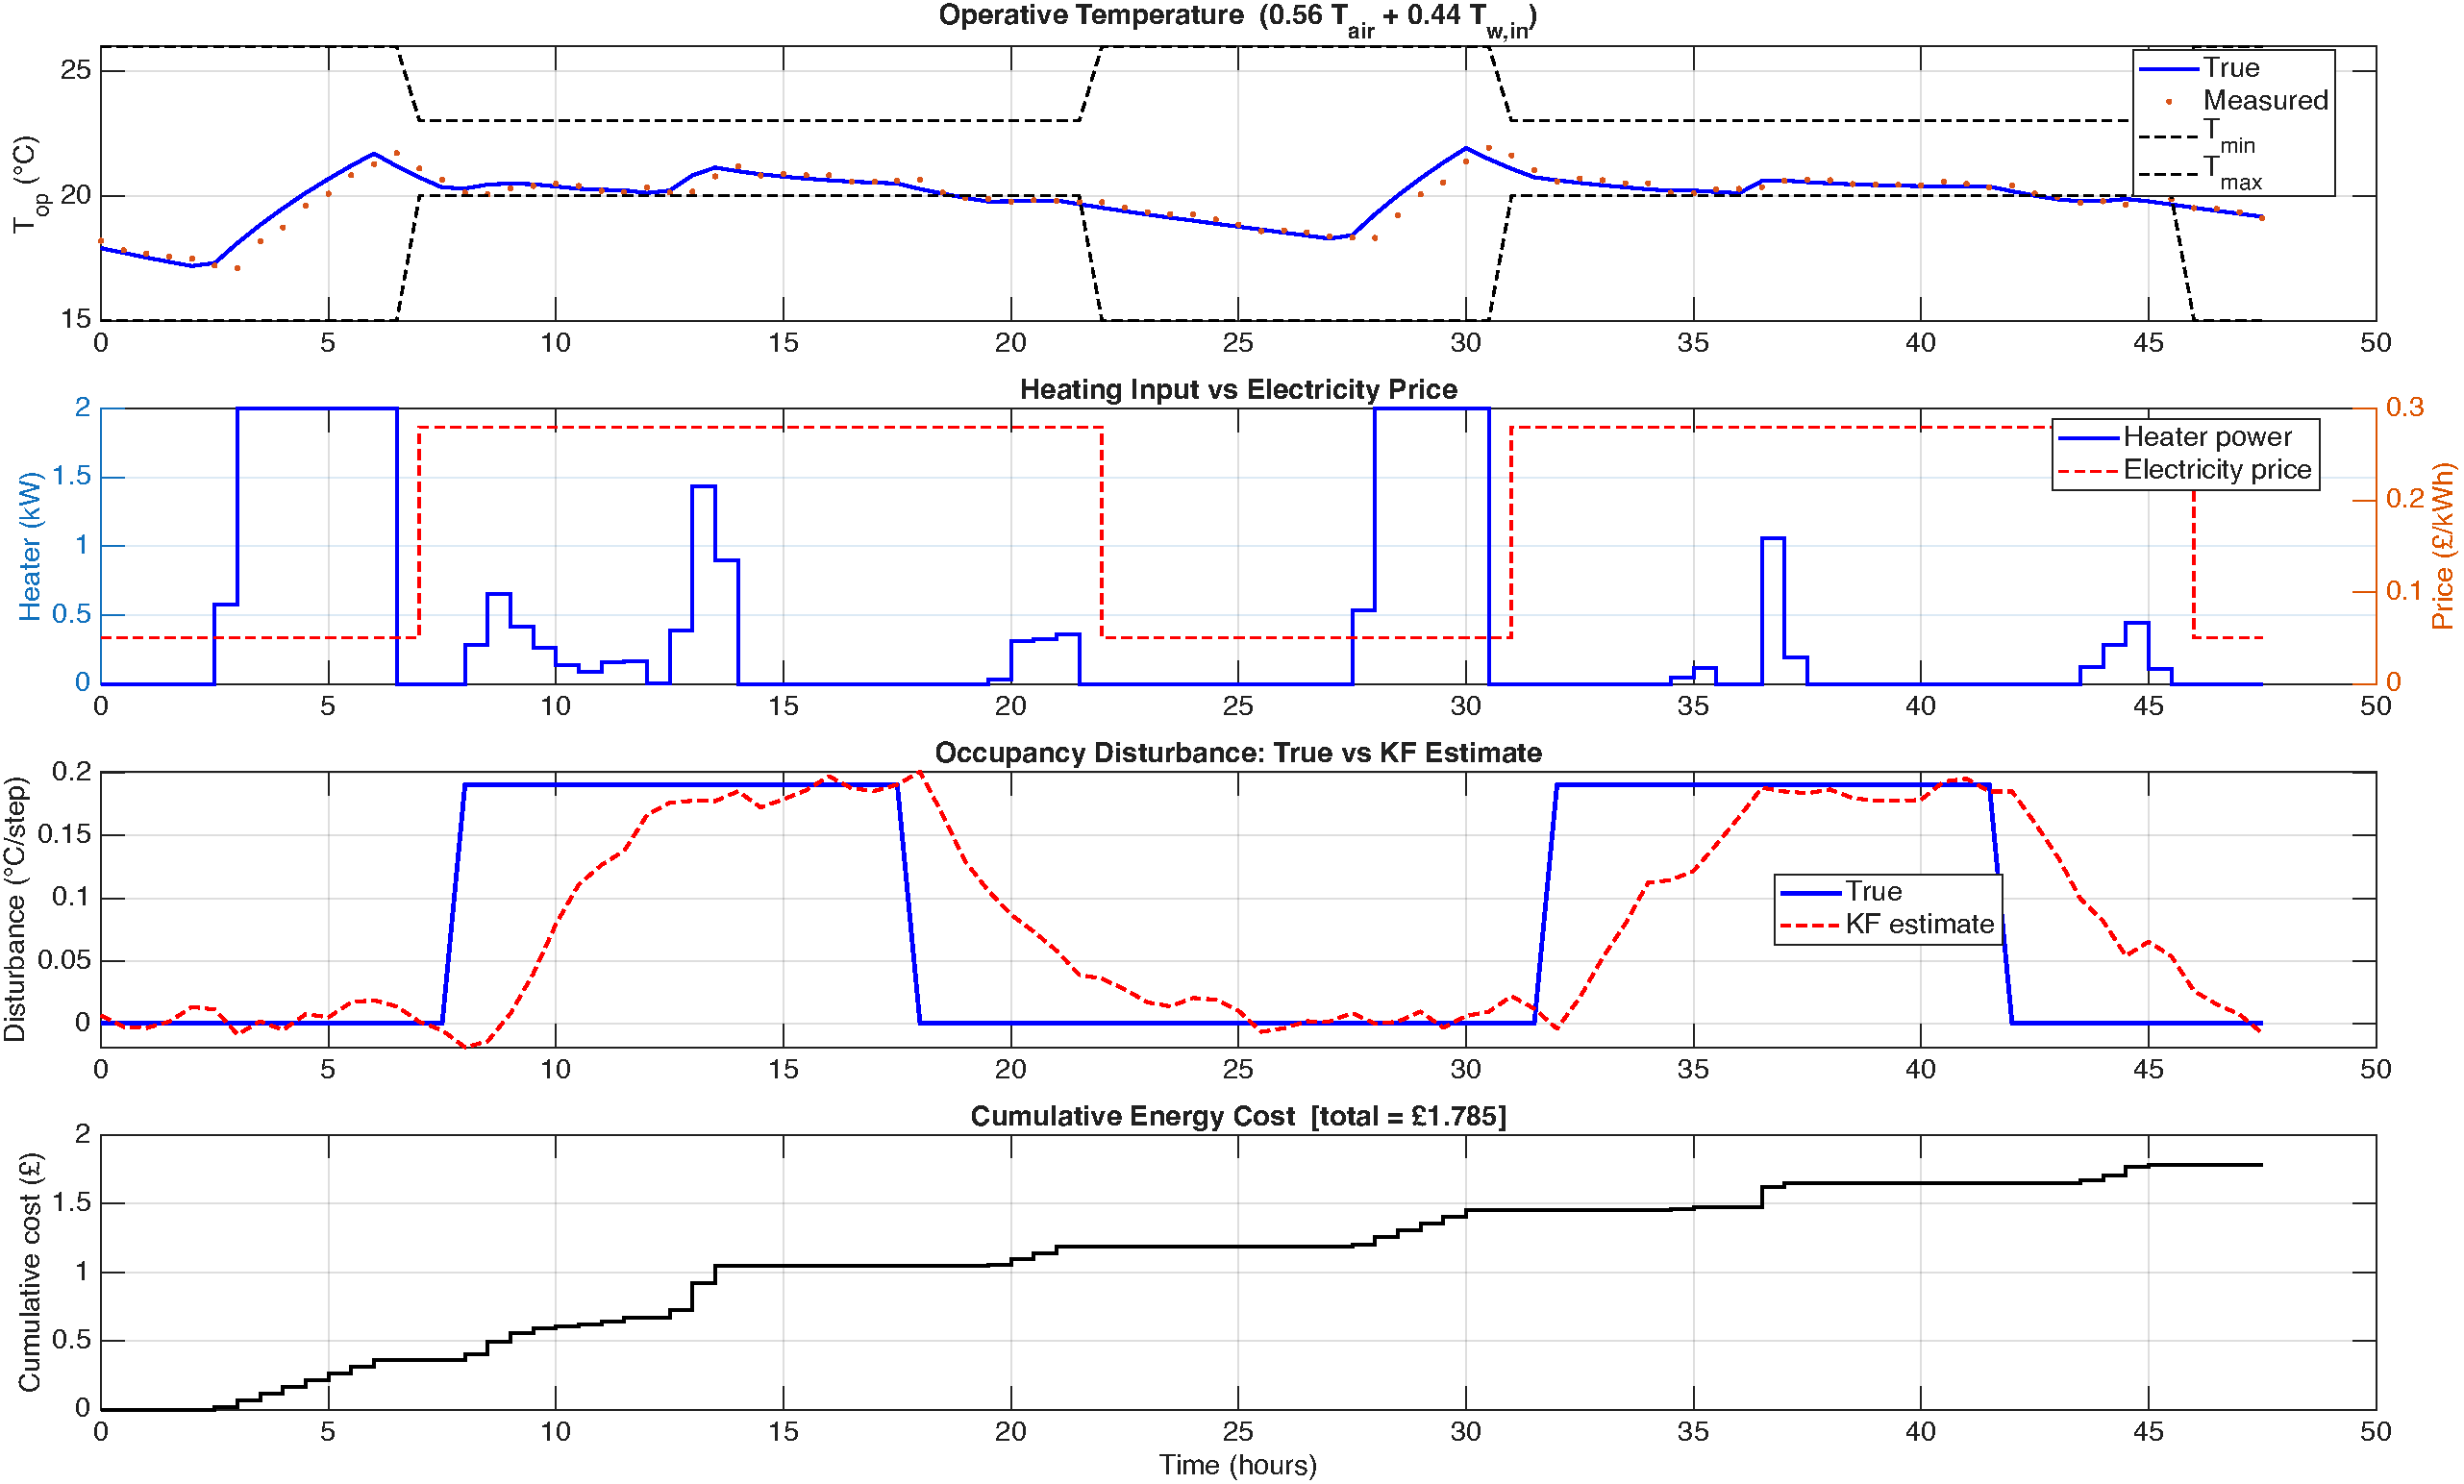
\includegraphics[width=0.9\linewidth]{Figures/hvac.pdf}
	\captionof{figure}{Closed-loop performance of the economic offset-free MPC for the
		single-zone building heating example over a 48-hour simulation.
		\textit{Top:} Operative temperature tracking the time-varying comfort
		region; the controller pre-heats during the cheap off-peak window before
		07:00 and reduces heating during the expensive daytime tariff.
		\textit{Second:} Heater power overlaid with the electricity price;
		the load-shifting behaviour is clearly visible.
		\textit{Third:} True occupancy disturbance versus the Kalman filter
		estimate; convergence is fast because $CB_w = 1$.
		\textit{Bottom:} Cumulative energy cost in GBP over the 48-hour horizon.}
	\label{fig:singlezone2}

\end{examplebox}

% ===================================================================
%  Example: Offset-free MPC for a 3-DOF Articulated Robot Manipulator
%  Drop this file into your chapter via \input{Example_3DOF_MPC}
%  Requires the preamble from Main.tex (tcolorbox, listings, tikz, etc.)
% ===================================================================

\begin{examplebox}{Offset-free MPC of a 3-DOF Articulated Robot Manipulator}
	
	% -------------------------------------------------------------------
	%  PART 1 — Problem Description
	% -------------------------------------------------------------------
	\textbf{\textsf{Problem Description}}
	
	Consider a three-degree-of-freedom (3-DOF) \emph{RRR} articulated robot manipulator
	operating in three-dimensional space. The three revolute joints are arranged as follows:
	joint~1 rotates about the vertical ($z$) axis (base yaw), whilst joints~2 and~3 rotate
	about parallel horizontal ($y$) axes (shoulder and elbow pitch, respectively). This
	configuration is representative of the positioning structure found in industrial serial
	manipulators.
	
	The control objective is to track piecewise-constant joint-angle references
	$r(t) \in \mathbb{R}^{3}$ in the presence of persistent disturbances (joint friction
	and unexpected payload changes) whilst respecting hard torque limits and soft joint-angle
	limits. An offset-free MPC strategy based on computed-torque feedback linearisation and
	an augmented Kalman filter (AKF) is employed.
	
	% -------------------------------------------------------------------
	%  PART 2 — Kinematic Configuration (TikZ)
	% -------------------------------------------------------------------
	\vspace{0.5em}
	\textbf{\textsf{Kinematic Configuration}}
	
	Figure~\ref{fig:3dof_arm} shows the side-view projection of the arm and the
	definition of the joint angles $q_1$, $q_2$, and $q_3$. The base yaw axis
	is perpendicular to the plane of the figure.
	
	\begin{figure}[H]
		\centering
		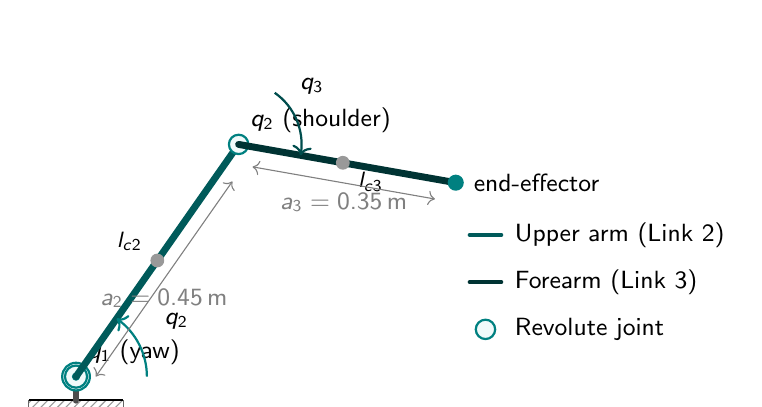
\begin{tikzpicture}[
			every node/.style={font=\small\sffamily},
			joint/.style={circle, draw=excolor, fill=exback, thick, minimum size=7pt, inner sep=0pt},
			link/.style={draw=black!70, line width=2.5pt, line cap=round},
			ground/.style={pattern=north east lines, pattern color=black!40, draw=black!60}
			]
			
			% --- Ground / base pedestal ---
			\fill[ground] (-0.6,-0.55) rectangle (0.6,-0.3);
			\draw[thick] (-0.6,-0.3) -- (0.6,-0.3);
			
			% --- Link lengths (display scale) ---
			% a2 = 0.45 m  →  3.6 units
			% a3 = 0.35 m  →  2.8 units
			% scale factor 8
			
			% --- Joint angles (display) ---
			\pgfmathsetmacro{\qTwo}{55}
			\pgfmathsetmacro{\qThree}{-65}
			
			% --- Joint 1 (origin, base yaw shown as cross-section circle) ---
			\coordinate (J1) at (0,0);
			\draw[link] (0,-0.3) -- (J1);
			\node[joint, minimum size=10pt] at (J1) {};
			\node[above right=1pt] at (J1) {$q_1$ (yaw)};
			
			% Yaw axis indicator
			\draw[thick, excolor] (J1) circle (4pt);
			\fill[excolor] (J1) circle (1.5pt);
			
			% --- Upper arm (Link 2) ---
			\coordinate (J2) at ($(J1) + (\qTwo:3.6)$);
			\draw[link, excolor!70!black] (J1) -- (J2);
			
			% Angle arc q2
			\draw[->, excolor, thick] (0.9,0) arc[start angle=0, end angle=\qTwo, radius=0.9];
			\node[right] at (1.0,0.7) {$q_2$};
			
			% COM marker link 2
			\coordinate (COM2) at ($(J1)!0.5!(J2)$);
			\fill[black!40] (COM2) circle (2.5pt);
			\node[above left, xshift=-2pt] at (COM2) {\footnotesize $l_{c2}$};
			
			% --- Joint 2 ---
			\node[joint] at (J2) {};
			\node[above right=1pt] at (J2) {$q_2$ (shoulder)};
			
			% --- Forearm (Link 3) ---
			\pgfmathsetmacro{\absThree}{\qTwo + \qThree}
			\coordinate (J3) at ($(J2) + (\absThree:2.8)$);
			\draw[link, excolor!40!black] (J2) -- (J3);
			
			% Angle arc q3
			\pgfmathsetmacro{\arcStart}{\qTwo}
			\pgfmathsetmacro{\arcEnd}{\qTwo + \qThree}
			\draw[->, excolor!60!black, thick]
			($(J2) + (\arcStart:0.8)$) arc[start angle=\arcStart, end angle=\arcEnd, radius=0.8];
			\node[right=4pt] at ($(J2) + (\arcStart:0.9)$) {$q_3$};
			
			% COM marker link 3
			\coordinate (COM3) at ($(J2)!0.48!(J3)$);
			\fill[black!40] (COM3) circle (2.5pt);
			\node[below right, xshift=2pt] at (COM3) {\footnotesize $l_{c3}$};
			
			% --- End-effector ---
			\node[joint, minimum size=5pt, fill=excolor] at (J3) {};
			\node[right=3pt] at (J3) {end-effector};
			
			% --- Dimension lines ---
			\draw[<->, gray, thin]
			($(J1)!0.08!(J2) + (-70:0.25)$) -- ($(J1)!0.92!(J2) + (-70:0.25)$)
			node[midway, below, gray] {$a_2 = 0.45\,\mathrm{m}$};
			
			\draw[<->, gray, thin]
			($(J2)!0.08!(J3) + ({\absThree-90}:0.25)$) -- ($(J2)!0.92!(J3) + ({\absThree-90}:0.25)$)
			node[midway, below, gray] {$a_3 = 0.35\,\mathrm{m}$};
			
			% --- Legend ---
			\draw[link, excolor!70!black, line width=1.5pt] (5.0,1.8) -- (5.4,1.8);
			\node[right] at (5.45,1.8) {\small Upper arm (Link 2)};
			
			\draw[link, excolor!40!black, line width=1.5pt] (5.0,1.2) -- (5.4,1.2);
			\node[right] at (5.45,1.2) {\small Forearm (Link 3)};
			
			\node[joint, minimum size=7pt] at (5.2, 0.6) {};
			\node[right] at (5.45, 0.6) {\small Revolute joint};
			
		\end{tikzpicture}
		\caption{Side-view projection of the 3-DOF RRR articulated arm.
			Joint~1 (base yaw) is perpendicular to the page; joints~2 and~3
			(shoulder and elbow pitch) lie in the plane shown.}
		\label{fig:3dof_arm}
	\end{figure}
	
	% -------------------------------------------------------------------
	%  PART 3 — Robot Parameters
	% -------------------------------------------------------------------
	\textbf{\textsf{Physical Parameters}}
	
	
	\begin{center}
		\captionof{table}{Parameters used in the simulation.}
		\begin{tabular}{llcc}
			\toprule
			Symbol & Description & Value & Unit \\
			\midrule
			$I_{z1}$  & Base yaw inertia (joint 1)         & 1.50  & kg\,m$^{2}$ \\
			$m_2$     & Mass of upper arm (link 2)          & 6.00  & kg          \\
			$a_2$     & Length of upper arm                  & 0.45  & m           \\
			$l_{c2}$  & COM distance from joint 2           & 0.22  & m           \\
			$I_2$     & Pitch inertia of link 2 about COM   & 0.15  & kg\,m$^{2}$ \\
			$m_3$     & Mass of forearm (link 3)            & 3.50  & kg          \\
			$a_3$     & Length of forearm                    & 0.35  & m           \\
			$l_{c3}$  & COM distance from joint 3           & 0.17  & m           \\
			$I_3$     & Pitch inertia of link 3 about COM   & 0.08  & kg\,m$^{2}$ \\
			$T_s$     & Sampling period                      & 0.02  & s           \\
			\bottomrule
		\end{tabular}
	\end{center}
	
	% -------------------------------------------------------------------
	%  PART 4 — Control Strategy
	% -------------------------------------------------------------------
	\vspace{0.4em}
	\textbf{\textsf{Control Technique: Computed-Torque MPC with Disturbance Observer}}
	
	The full nonlinear robot dynamics are:
	\begin{equation}
		M(q)\,\ddot{q} + Cor(q,\dot{q})\,\dot{q} + G(q) = \tau + d_{\tau},
		\label{eq:robot_dyn}
	\end{equation}
	where $q \in \mathbb{R}^{3}$ are the joint angles, $M(q)$ is the symmetric
	positive-definite inertia matrix, $Cor(q,\dot{q})\dot{q}$ collects Coriolis and
	centrifugal torques, $G(q)$ is the gravity vector, $\tau$ is the applied torque, and
	$d_{\tau} \in \mathbb{R}^{3}$ represents lumped torque-space disturbances
	(friction, payload) in~[Nm].
	
	\emph{Computed-torque (CT) feedback linearisation} is applied by choosing:
	\begin{equation}
		\tau = M(q)\,v + Cor(q,\dot{q})\,\dot{q} + G(q),
		\label{eq:ct_law}
	\end{equation}
	which reduces~\eqref{eq:robot_dyn} to three decoupled double integrators,
	one per joint:
	\begin{equation}
		\ddot{q} = v + \underbrace{M(q)^{-1}\,d_{\tau}}_{\displaystyle d},
		\label{eq:double_int}
	\end{equation}
	where $d \triangleq M(q)^{-1}\,d_{\tau} \in \mathbb{R}^{3}$ is the
	\emph{acceleration-space disturbance}~[rad/s$^{2}$].
	Because the MPC and observer operate entirely in the linearised
	(virtual-acceleration) domain, $d$~is the natural disturbance variable
	for the remainder of the formulation.
	If the physical torque-space disturbance is needed, it can be recovered as
	$\hat{d}_{\tau} = M(q)\,\hat{d}$.
	
	Defining the state $x = [q^{\top},\,\dot{q}^{\top}]^{\top} \in \mathbb{R}^{6}$,
	the linearised continuous-time plant is:
	\begin{equation}
		\dot{x} =
		\underbrace{\begin{bmatrix}0 & I \\ 0 & 0\end{bmatrix}}_{A_c}x +
		\underbrace{\begin{bmatrix}0 \\ I\end{bmatrix}}_{B_c}v, \qquad
		y = \underbrace{\begin{bmatrix}I & 0\end{bmatrix}}_{C}\,x,
		\label{eq:lin_plant}
	\end{equation}
	which is discretised exactly via zero-order hold at $T_s = 0.02$\,s to give
	$(A,\,B,\,C)$. The entire control scheme is shown in Figure~\ref{fig:CTMPC_robot_block_diagram}.
	
	% -------------------------------------------------------------------
	%  PART 5 — MPC Formulation
	% -------------------------------------------------------------------
	\vspace{0.4em}
	\textbf{\textsf{MPC Formulation}}
	
	\emph{Augmented observer for offset-free control.}
	A random-walk model $d_{k+1} = d_k$ for the acceleration-space disturbance
	is appended to the plant state,
	yielding the augmented system $z = [x^{\top},\,d^{\top}]^{\top} \in \mathbb{R}^{9}$:
	\begin{equation}
		\begin{bmatrix}x_{k+1}\\d_{k+1}\end{bmatrix}
		=
		\underbrace{\begin{bmatrix}A & B \\ 0 & I\end{bmatrix}}_{A_{\mathrm{aug}}}
		\begin{bmatrix}x_k\\d_k\end{bmatrix}
		+
		\underbrace{\begin{bmatrix}B\\0\end{bmatrix}}_{B_{\mathrm{aug}}}v_k, \qquad
		y_k =
		\underbrace{\begin{bmatrix}C & 0\end{bmatrix}}_{C_{\mathrm{aug}}}
		\begin{bmatrix}x_k\\d_k\end{bmatrix}.
		\label{eq:aug_sys}
	\end{equation}
	Note that $d$ enters the state equation through $B$ (the same input matrix as $v$),
	confirming that it represents the disturbance in virtual-acceleration
	units~[rad/s$^{2}$], not in torque units~[Nm].
	The observer gain $L$ is obtained from the discrete algebraic Riccati equation
	(DARE) with process noise covariance
	$Q = \mathrm{diag}(10^{-6}I_6,\;10^{-3}I_3)$ and measurement noise
	covariance $R = \sigma_{\mathrm{enc}}^{2}\,I_3$ where
	$\sigma_{\mathrm{enc}} = 0.05^{\circ}$ (encoder standard deviation). The controller can only access the measurements of angular positions, $q$. Therefore, $C=\begin{bmatrix}
	I_{3\times 3} & 0_{3\times 3}
	\end{bmatrix}$
	
	\emph{Target calculator.}
	At steady state, $x_{k+1} = x_k = x_{\mathrm{ss}}$ and $y_{\mathrm{ss}} = r_k$,
	so the pair $(x_{\mathrm{ss}},\,v_{\mathrm{ss}})$ satisfies:
	\begin{equation}
		\begin{bmatrix}I - A & -B \\ C & 0\end{bmatrix}
		\begin{bmatrix}x_{\mathrm{ss}} \\ v_{\mathrm{ss}}\end{bmatrix}
		=
		\begin{bmatrix}B\,\hat{d}_k \\ r_k\end{bmatrix}.
		\label{eq:target}
	\end{equation}
	This ensures that the MPC drives the plant to the reference with zero steady-state
	offset despite the persistent acceleration-space disturbance estimate
	$\hat{d}_k$~[rad/s$^{2}$].
	
	\emph{Deviation-form optimal control problem.}
	Let $\delta x_k = x_k - x_{\mathrm{ss}}$ and $\delta v_k = v_k - v_{\mathrm{ss}}$.
	The QP solved at each sampling instant is:
	\begin{equation}
		\begin{aligned}
			\min_{\{\delta v_k\},\{s_k\}}\;\;
			&\sum_{k=0}^{N-1}\!\left[
			\delta y_k^{\top} Q_y\,\delta y_k
			+ \delta v_k^{\top} R\,\delta v_k
			+ \rho\,s_k^{\top}s_k
			\right]
			+ \delta x_N^{\top} P_N\,\delta x_N \\[4pt]
			\text{subject to}\;\;
			&\delta x_{k+1} = A\,\delta x_k + B\,\delta v_k,
			\quad \delta x_0 = \hat{x}_k - x_{\mathrm{ss}},\\
			&v_{\min} \leq \delta v_k + v_{\mathrm{ss}} \leq v_{\max},\\
			&y_{\min} - s_k \leq C(\delta x_k + x_{\mathrm{ss}}) \leq y_{\max} + s_k,\\
			&s_k \geq 0, \quad k = 0, \ldots, N-1,
		\end{aligned}
		\label{eq:ocp}
	\end{equation}
	where $\delta y_k = C\,\delta x_k$, $P_N$ is the terminal LQR cost matrix (from the
	DARE for $(A,B,Q_{\mathrm{mpc}},R)$), and $s_k \in \mathbb{R}^{3}$ are slack
	variables that soften the joint-angle constraints.
	
	The MPC tuning parameters are summarised in Table~\ref{tab:robot_parameters}.
	
	
	\captionof{table}{Robot parameters.}\label{tab:robot_parameters}
	\begin{center}
		\begin{tabular}{llc}
			\toprule
			Parameter & Description & Value \\
			\midrule
			$N$        & Prediction horizon                        & 15 \\
			$Q_y$      & Output tracking weight                    & $200\,I_3$ \\
			$R$        & Control effort weight                     & $0.1\,I_3$ \\
			$\rho$     & Soft-constraint penalty                   & $10^{6}$ \\
			$v_{\min}$ & Virtual acceleration lower bound          & $-50\,\mathrm{rad/s}^2$ \\
			$v_{\max}$ & Virtual acceleration upper bound          & $+50\,\mathrm{rad/s}^2$ \\
			$y_{\min}$ & Joint angle lower limits                  & $[-170^\circ,\,-90^\circ,\,-135^\circ]^{\top}$ \\
			$y_{\max}$ & Joint angle upper limits                  & $[+170^\circ,\,+90^\circ,\,+135^\circ]^{\top}$ \\
			$\tau_{\max}$ & Actuator torque limits (absolute)      & $[150,\,120,\,60]\,\mathrm{Nm}$ \\
			\bottomrule
		\end{tabular}
	\end{center}
	
	
	\begin{center}
		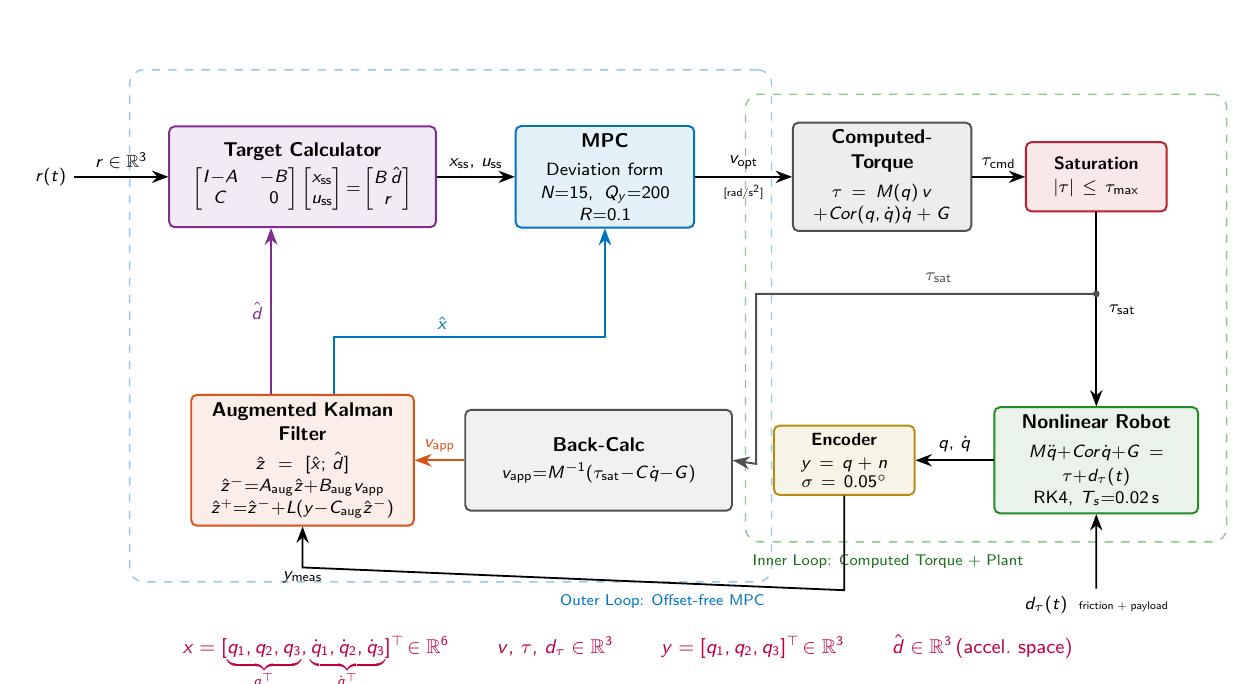
\begin{tikzpicture}[scale=0.8, transform shape]
			
			\tikzset{
				block/.style={
					draw, rectangle, rounded corners=2pt,
					minimum height=1.4cm, minimum width=2.8cm,
					text width=2.6cm, align=center,
					font=\small\sffamily, line width=0.7pt,
				},
				wideblock/.style={
					draw, rectangle, rounded corners=2pt,
					minimum height=1.6cm, minimum width=3.5cm,
					text width=4cm, align=center,
					font=\small\sffamily, line width=0.7pt,
				},
				smallblock/.style={
					draw, rectangle, rounded corners=2pt,
					minimum height=1.1cm, minimum width=2.2cm,
					text width=2.0cm, align=center,
					font=\footnotesize\sffamily, line width=0.7pt,
				},
				arr/.style={-Stealth, line width=0.65pt},
				sig/.style={font=\footnotesize\sffamily},
				sm/.style={font=\footnotesize},
			}
			
			% =====================================================================
			%  ROW 1 (y=0):  ref -> Target -> MPC -> CT -> Sat
			% =====================================================================
			
			\node[sig] (ref) at (-1, 0) {$r(t)$};
			
			\node[wideblock, fill=targetpurp!10, draw=targetpurp]
			(target) at (3., 0) {%
				\textbf{Target Calculator}\\[2pt]
				{\footnotesize $\begin{bmatrix} I{-}A & -B \\ C & 0 \end{bmatrix}
					\begin{bmatrix} x_\mathrm{ss} \\ u_\mathrm{ss} \end{bmatrix}
					{=} \begin{bmatrix} B\,\hat{d} \\ r \end{bmatrix}$}
			};
			
			\node[block, fill=mpcblue!10, draw=mpcblue]
			(mpc) at (7.8, 0) {%
				\textbf{MPC}\\[2pt]
				{\footnotesize Deviation form}\\[-1pt]
				{\footnotesize $N{=}15,\; Q_y{=}200$}\\[-1pt]
				{\footnotesize $R{=}0.1$}
			};
			
			\node[block, fill=ctgray!10, draw=ctgray]
			(ct) at (12.2, 0) {%
				\textbf{Computed-Torque}\\[2pt]
				{\footnotesize $\tau = M(q)\,v$}\\[-1pt]
				{\footnotesize $+ Cor(q,\dot{q})\dot{q} + G$}
			};
			
			\node[smallblock, fill=satred!10, draw=satred]
			(sat) at (15.6, 0) {%
				\textbf{Saturation}\\[1pt]
				{\footnotesize $|\tau| \leq \tau_{\max}$}
			};
			
			% =====================================================================
			%  ROW 2 (y=-4.5):  AKF --- BackCalc --- Sensor --- Plant
			% =====================================================================
			
			\node[wideblock, fill=obsvorange!10, draw=obsvorange,
			minimum height=1.8cm, minimum width=3.5cm, text width=3.3cm]
			(akf) at (3., -4.5) {%
				\textbf{Augmented Kalman}\\
				\textbf{Filter}\\[2pt]
				{\footnotesize $\hat{z} = [\hat{x};\, \hat{d}]$}\\[-1pt]
				{\footnotesize $\hat{z}^- {=} A_\mathrm{aug}\hat{z} {+} B_\mathrm{aug} v_\mathrm{app}$}\\[-1pt]
				{\footnotesize $\hat{z}^+ {=} \hat{z}^- {+} L(y{-}C_\mathrm{aug}\hat{z}^-)$}
			};
			
			\node[wideblock, fill=ctgray!8, draw=ctgray]
			(backcalc) at (7.7, -4.5) {%
				\textbf{Back-Calc}\\[1pt]
				{\footnotesize $v_\mathrm{app} {=} M^{-1}(\tau_\mathrm{sat}{-}C\dot{q}{-}G)$}
			};
			
			\node[smallblock, fill=sensorgold!10, draw=sensorgold]
			(sensor) at (11.6, -4.5) {%
				\textbf{Encoder}\\[1pt]
				{\footnotesize $y = q + n$}\\[-1pt]
				{\footnotesize $\sigma = 0.05^\circ$}
			};
			
			\node[wideblock, fill=plantgreen!10, draw=plantgreen,
			minimum width=3.2cm, text width=3.0cm]
			(plant) at (15.6, -4.5) {%
				\textbf{Nonlinear Robot}\\[2pt]
				{\footnotesize $M\ddot{q} {+} Cor\dot{q} {+} G= \tau {+} d_\tau(t)$}\\[-1pt]
				{\footnotesize RK4, $T_s{=}0.02\,$s}
			};
			
			% Disturbance input (from below)
			\node[sig] (dist) at (15.6, -6.8) {$d_{\tau}(t)$\; {\tiny friction + payload}};
			
			% =====================================================================
			%  FORWARD PATH  (Row 1, left to right)
			% =====================================================================
			
			\draw[arr] (ref) -- (target)
			node[midway, above, sig] {$r \in \mathbb{R}^3$};
			
			\draw[arr] (target) -- (mpc)
			node[midway, above, sm] {$x_\mathrm{ss},\, u_\mathrm{ss}$};
			
			\draw[arr] (mpc) -- (ct)
			node[midway, above, sm] {$v_\mathrm{opt}$}
			node[midway, below, sig] {\tiny [rad/s$^2$]};
			
			\draw[arr] (ct) -- (sat)
			node[midway, above, sm] {$\tau_\mathrm{cmd}$};
			
			% =====================================================================
			%  Sat -> Plant  (vertical connector between rows)
			% =====================================================================
			
			\draw[arr] (sat.south) -- (plant.north)
			node[midway, right, sm, xshift=2pt] {$\tau_\mathrm{sat}$};
			
			% Disturbance -> Plant
			\draw[arr] (dist) -- (plant.south);
			
			% =====================================================================
			%  ROW 2 FEEDBACK  (right to left)
			% =====================================================================
			
			% Plant -> Sensor  (straight horizontal)
			\draw[arr] (plant.west) -- (sensor.east)
			node[midway, above, sm] {$q,\, \dot{q}$};
			
			% Sensor -> AKF  (route below Row 2 blocks to avoid crossing Back-Calc)
			%   sensor.south -> down -> left -> up -> akf.south
			\draw[arr]
			(sensor.south) -- ++(0, -1.5)
			-- ($(akf.south) + (0., -0.65)$)
			-- ($(akf.south) $)
			node[pos=0.1, below, sm] {$y_\mathrm{meas}$};
			
			% Back-Calc -> AKF  (straight horizontal, no conflict now)
			\draw[arr, obsvorange, line width=0.7pt]
			(backcalc.west) -- (akf.east)
			node[midway, above, sm, text=obsvorange] {$v_\mathrm{app}$};
			
			% =====================================================================
			%  tau_sat branch -> Back-Calc  (from the vertical sat-plant line)
			% =====================================================================
			
			%Branch from sat->plant vertical line: left, down, left into backcalc.east
			\coordinate (tau_branch) at ($(sat.south)!0.42!(plant.north)$);
			\draw[arr, ctgray, line width=0.7pt]
			(tau_branch) -- ++(-5.4, 0)       % left (to x ≈ 10.2, between sensor & backcalc)
			-- ++(0, -2.7)                     % down to backcalc row
			-- (backcalc.east);                % left into backcalc
			\node[sm, text=ctgray] at ($(tau_branch) + (-2.5, 0.25)$) {$\tau_\mathrm{sat}$};
			\fill[ctgray] (tau_branch) circle (1.5pt);
			
			% =====================================================================
			%  ROW 2 -> ROW 1  (AKF estimates fed upward)
			% =====================================================================
			
			% d_hat:  AKF -> Target  (left side, straight up)
			\draw[arr, targetpurp, line width=0.7pt]
			($(akf.north) + (-0.5, 0)$) -- ($(target.south) + (-0.5, 0)$)
			node[midway, left, sm, text=targetpurp] {$\hat{d}$};
			
			% x_hat:  AKF -> MPC  (right side of AKF, up then right to MPC)
			\draw[arr, mpcblue, line width=0.7pt]
			($(akf.north) + (0.5, 0)$) -- ++(0, 0.9)
			-| (mpc.south)
			node[pos=0.20, above, sm, text=mpcblue] {$\hat{x}$};
			
			% =====================================================================
			%  DASHED LOOP BOXES
			% =====================================================================
			
			\begin{scope}[on background layer]
				\node[draw=mpcblue!40, dashed, line width=0.5pt, rounded corners=5pt,
				inner xsep=14pt, inner ysep=20pt,
				fit=(target)(mpc)(akf)(backcalc),
				label={[font=\scriptsize\sffamily, text=mpcblue, anchor=north east, yshift=-2pt]
					south east:Outer Loop: Offset-free MPC}] {};
				
				\node[draw=plantgreen!50, dashed, line width=0.5pt, rounded corners=5pt,
				inner xsep=10pt, inner ysep=10pt,
				fit=(ct)(sat)(plant)(sensor),
				label={[font=\scriptsize\sffamily, text=plantgreen!80!black, anchor=north west, yshift=-2pt]
					south west:Inner Loop: Computed Torque + Plant}] {};
			\end{scope}
			
			% =====================================================================
			%  TITLE & LEGEND
			% =====================================================================
			
			
			\node[font=\small\sffamily, text=purple, anchor=center]
			at ($(current bounding box.south) + (0, -0.65)$)
			{$x = [\underbrace{q_1,q_2,q_3}_{q^\top},\underbrace{\dot{q}_1,\dot{q}_2,\dot{q}_3}_{\dot q^\top}]^\top \!\in \mathbb{R}^6$
				\qquad
				$v,\,\tau,\,d_{\tau} \in \mathbb{R}^3$
				\qquad
				$y = [q_1,q_2,q_3]^\top \!\in \mathbb{R}^3$
				\qquad
				$\hat{d} \in \mathbb{R}^3$\,(accel.\ space)
			};
			
		\end{tikzpicture}
		\captionof{figure}{Block diagram of the computed-torque based feedback linearisation + MPC scheme.
			The disturbance $d_{\tau}$~[Nm] acts on the physical plant; after computed-torque
			cancellation the observer estimates the acceleration-space disturbance
			$\hat{d} = M^{-1}\hat{d}_{\tau}$~[rad/s$^{2}$].}
		\label{fig:CTMPC_robot_block_diagram}
	\end{center}
	
	\begin{lstlisting}[language=MATLAB]
	clear; clc; close all; rng(1);
	
	%% ===================================================================
	%  Offset-free MPC for a 3-DOF Spatial Articulated Robot Manipulator
	% ===================================================================
	
	%% 1. Robot Physical Parameters
	% --- Base (Link 1) -----------------------------------------------
	Iz1 = 1.50;          % z-axis inertia
	
	% --- Upper arm (Link 2) ------------------------------------------
	m2  = 6.00;                 % mass [kg]
	a2  = 0.45;                  % length [m]
	lc2 = 0.22;                   % COM distance from joint 2 
	I2  = 0.15;                     % pitch inertia about COM
	
	% --- Forearm (Link 3) --------------------------------------------
	m3  = 3.50;       % mass [kg]
	a3  = 0.35;        % length [m]  (geometry only)
	lc3 = 0.17;         % COM distance from joint 3
	I3  = 0.08;         % pitch inertia about COM 
	
	g_acc = 9.81;            % gravity
	Ts    = 0.02;                % sample time [s]  (50 Hz)
	
	nq = 3;       % degrees of freedom
	nx = 2*nq;    % state  [q1 q2 q3  dq1 dq2 dq3]
	nu = nq;      % virtual inputs  
	ny = nq;      % measured outputs (joint angles)
	nd = nu;      % one disturbance per joint
	
	% Dynamics function handles
	robot_M = @(q) inertia_matrix_3dof (q, m2,m3,a2,lc2,lc3,Iz1,I2,I3);
	robot_C = @(q,dq) coriolis_matrix_3dof(q, dq,  m2,m3,a2,lc2,lc3);
	robot_G = @(q) gravity_vector_3dof (q, m2,m3,lc2,a2,lc3,g_acc);
	
	%% 2. Linearised Plant 
	Ac  = [zeros(nq), eye(nq); zeros(nq), zeros(nq)];
	Bc  = [zeros(nq); eye(nq)];
	Cc  = [eye(nq),   zeros(nq)];   % measure joint angles only
	
	sys_d = c2d(ss(Ac, Bc, Cc, 0), Ts, 'zoh');
	A     = sys_d.A;
	B     = sys_d.B;
	C     = sys_d.C;
	
	% 3. Augmented Observer
	%
	%  Augmented state:  z = [x; d],   d_{k+1} = d_k
	%
	%  A_aug = [A   B;  0   I]   B_aug = [B;  0]   C_aug = [C  0]
	%           		             
	nz    = nx + nd;
	A_aug = [A,            B*eye(nd);
	zeros(nd,nx), eye(nd)  ];
	B_aug = [B; zeros(nd,nu)];
	C_aug = [C, zeros(ny,nd)];
	
	% Kalman filter noise covariances
	sigma_enc = deg2rad(0.05);                      
	R_kf      = sigma_enc^2 * eye(ny);
	Q_state   = 1e-6 * eye(nx);
	Q_dist    = 1e-3 * eye(nd);
	Q_kf      = blkdiag(Q_state, Q_dist);
	
	[P_ss, ~, ~] = dare(A_aug', C_aug', Q_kf, R_kf);
	L = P_ss * C_aug' / (C_aug * P_ss * C_aug' + R_kf);
	
	fprintf('\nObserver gain L (first 3 rows shown):\n'); disp(L(1:3,:));
	
	%% 4. Target Calculator
	%  Solve  [I-A  -B; C  0]  [x_ss; u_ss] = [B d; ref]
	M_target = [eye(nx)-A, -B; C, zeros(ny,nu)];
	if rank(M_target) < nx+nu
		error('Target calculator matrix is rank-deficient.');
	end
	
	% 5. MPC Formulation  (YALMIP + quadprog, deviation form)
	N    = 15;      % prediction horizon
	q_y  = 200;     % output tracking weight
	R_u  = 0.10;    % control effort weight
	rho  = 1e6;     % soft-constraint penalty
	
	Q_mpc = C' * (q_y*eye(ny)) * C;
	[P_N, ~, ~] = dare(A, B, Q_mpc, R_u*eye(nu));   % terminal (LQR) cost
	
	du    = sdpvar(nu, N,   'full');
	dx    = sdpvar(nx, N+1, 'full');
	slack = sdpvar(ny, N,   'full');
	
	% Parameters updated each step
	x_hat = sdpvar(nx, 1);
	x_ss  = sdpvar(nx, 1);
	u_ss  = sdpvar(nu, 1);
	
	% ---- Physical bounds ------
	% Virtual acceleration bounds [rad/s^2]  (after computed-torque cancellation)
	v_min = -50*ones(nu,1);    v_max = 50*ones(nu,1);
	
	% Joint angle limits [rad]
	y_min = deg2rad([-170; -90; -135]);
	y_max = deg2rad([ 170;  90;  135]);
	
	% ---- Optimal Control Problem ---------------------------------------
	obj  = 0;
	cons = [dx(:,1) == x_hat - x_ss];
	
	for k = 1:N
		cons = [cons, dx(:,k+1) == A*dx(:,k) + B*du(:,k)];
		
		dy_k = C * dx(:,k);
		obj  = obj + dy_k'*(q_y*eye(ny))*dy_k ...
				+ du(:,k)'*(R_u*eye(nu))*du(:,k) ...
				+ rho * slack(:,k)' * slack(:,k);
		
		v_abs = du(:,k) + u_ss;
		y_abs = C * (dx(:,k) + x_ss);
		
		cons = [cons, v_min <= v_abs <= v_max];
		cons = [cons, y_min - slack(:,k) <= y_abs <= y_max + slack(:,k)];
		cons = [cons, slack(:,k) >= 0];
	end
	obj = obj + dx(:,N+1)' * P_N * dx(:,N+1);
	
	ops      = sdpsettings('solver','quadprog','verbose',0);
	mpc_ctrl = optimizer(cons, obj, ops, {x_hat, x_ss, u_ss}, {du(:,1), slack(:,1)});
	
	fprintf('MPC compiled (N=%d, q_y=%.0f, R=%.3f, nq=%d).\n', N, q_y, R_u, nq);
	
	%% 6. Simulation Setup
	T_sim = 600;
	t_vec = (0:T_sim-1) * Ts;
	
	% True initial state  (robot at rest, slightly off-home)
	q_true  = [deg2rad(-15); deg2rad(25); deg2rad(-50)];
	dq_true = zeros(nq, 1);
	
	% Observer initial state  (matched to true state - avoids transient d spike)
	z_hat     = [q_true; dq_true; zeros(nd,1)];
	v_applied = zeros(nu, 1);
	
	% ---- Reference trajectory  [rad] -----------------------------------
	%  Six evenly-timed segments; each joint commanded independently.
	ref_signal = zeros(ny, T_sim);
	
	% Joint 1 - base yaw (5 segments x 120 steps = 600)
	ref_signal(1,:) = [repmat(deg2rad(  0), 1, 120), ...
	repmat(deg2rad( 45), 1, 120), ...
	repmat(deg2rad(-30), 1, 120), ...
	repmat(deg2rad( 60), 1, 120), ...
	repmat(deg2rad(  0), 1, 120)];
	
	% Joint 2 shoulder pitch (4 segments)
	ref_signal(2,:) = [repmat(deg2rad( 30), 1, 150), ...
	repmat(deg2rad( 60), 1, 150), ...
	repmat(deg2rad( 20), 1, 150), ...
	repmat(deg2rad( 50), 1, 150)];
	
	% Joint 3  elbow pitch (4 segments)
	ref_signal(3,:) = [repmat(deg2rad(-60), 1, 100), ...
	repmat(deg2rad(-30), 1, 150), ...
	repmat(deg2rad(-90), 1, 150), ...
	repmat(deg2rad(-45), 1, 200)];
	
	% ---- True disturbances  [Nm] (friction + sudden payload step) ------
	%  Constant friction bias on all joints; extra load added at t = 7 s
	d_true            = zeros(nd, T_sim);
	d_true(:, 1:end)  = repmat([0.50;  -0.30;  0.20], 1, T_sim);      % friction
	d_true(:, 351:end)= d_true(:,351:end) ...
	+ repmat([2.00;   1.50;  0.80], 1, T_sim-350);   % payload
	
	% ---- Measurement noise (encoder ~0.05 deg) ----------------------------
	sigma_y = deg2rad(0.05) * ones(ny, 1);
	
	% ---- Log arrays ----------------------------------------------------
	log_q          = zeros(ny, T_sim);
	log_q_ref      = zeros(ny, T_sim);
	log_tau        = zeros(nu, T_sim);
	log_v          = zeros(nu, T_sim);
	log_d_hat      = zeros(nd, T_sim);
	log_d_true_acc = zeros(nd, T_sim);   % true disturbance in [rad/s^2] = M^{-1} d_Nm
	log_slack      = zeros(ny, T_sim);
	
	fprintf('Simulation: %d steps, Ts=%.3f s, duration=%.1f s\n', ...
	T_sim, Ts, T_sim*Ts);
	tic;
	
	%% 7. Simulation Loop
	for t = 1:T_sim
	
		ref = ref_signal(:, t);
		
		% ==== A.  Plant output (angle measurement) ======================
		y_true = q_true;
		y_meas = y_true + sigma_y .* randn(ny, 1);
		
		% ==== B.  Augmented Kalman Filter ===============================
		z_pred = A_aug * z_hat + B_aug * v_applied;
		z_hat  = z_pred + L * (y_meas - C_aug * z_pred);
		
		x_hat_k = z_hat(1:nx);
		d_hat_k = z_hat(nx+1:end);
		
		% ==== C.  Target Calculator =====================================
		rhs     = [B * d_hat_k; ref];
		targets = M_target \ rhs;
		x_ss_k  = targets(1:nx);
		u_ss_k  = targets(nx+1:end);
		
		% ==== D.  MPC (deviation-form QP) ===============================
		[sol, diag_flag] = mpc_ctrl{x_hat_k, x_ss_k, u_ss_k};
		
		if diag_flag == 0
			dv_opt    = full(sol{1});
			slack_now = full(sol{2});
		else
			warning('MPC infea at t=%d (code %d). Holding u_ss.', t, diag_flag);
			dv_opt    = zeros(nu, 1);
			slack_now = NaN(ny, 1);
		end
		
		v_opt = dv_opt + u_ss_k;   % total virtual acceleration command 
		
		% ==== E.  Computed-Torque Law (exact feedback linearisation) ====
		%
		%
		
		M_mat = robot_M(q_true);
		C_vec = robot_C(q_true, dq_true) * dq_true;
		G_vec = robot_G(q_true);
		
		tau_cmd = M_mat * v_opt + C_vec + G_vec;
		
		% Saturate to physical actuator limits [Nm]
		tau_max = [150; 120; 60];
		tau_min = -tau_max;
		tau_cmd = min(max(tau_cmd, tau_min), tau_max);
		
		% Actual virtual input after saturation (fed back to observer)
		v_applied = M_mat \ (tau_cmd - C_vec - G_vec);
		
		% ==== F.  True Plant Integration (RK4, full nonlinear model) ====
		x_rob  = [q_true; dq_true];
		x_next = rk4_robot(x_rob, tau_cmd, d_true(:,t), Ts, ...
		robot_M, robot_C, robot_G, nq);
		q_true  = x_next(1:nq);
		dq_true = x_next(nq+1:end);
		
		% ==== G.  Logging ===============================================
		log_q(:,t)          = y_true;
		log_q_ref(:,t)      = ref;
		log_tau(:,t)        = tau_cmd;
		log_v(:,t)          = v_opt;
		log_d_hat(:,t)      = d_hat_k;
		log_d_true_acc(:,t) = M_mat \ d_true(:,t);  
		log_slack(:,t)      = slack_now;
	end
	
	elapsed = toc;
	fprintf('Done.  Wall-clock: %.2f s  (%.1f ms/step)\n', ...
	elapsed, elapsed/T_sim*1e3);
	
	
	
	%% ===================================================================
	%%  LOCAL FUNCTIONS
	%% ===================================================================
	
	% ------------------------------------------------------------------ %
	function M = inertia_matrix_3dof(q, m2, m3, a2, lc2, lc3, Iz1, I2, I3)
		% 3 x 3 symmetric positive-definite inertia matrix of the 3-DOF RRR arm.
		%
		%  Block-diagonal structure (q1 decoupled from q2,q3):
		%    M = diag( M11(q2,q3) , [M22 M23; M23 M33](q3) )
		%
		%  Derived via Lagrangian mechanics (Christoffel-symbol formulation).
		%  The block-diagonal structure follows from the perpendicular
	
		c2  = cos(q(2));
		c3  = cos(q(3));
		c23 = cos(q(2) + q(3));
		h   = m3 * a2 * lc3;                    
		
		R3  = a2*c2 + lc3*c23;                   % horizontal reach of link-3 COM
		
		M11 = Iz1 + I2 + I3 + m2*(lc2*c2)^2 + m3*R3^2;
		M22 = (I2 + m2*lc2^2) + (I3 + m3*lc3^2) + m3*a2^2 + 2*h*c3;
		M23 = (I3 + m3*lc3^2) + h*c3;
		M33 = I3 + m3*lc3^2;
		
		M = [M11, 0,   0  ;
				0, M22, M23 ;
				0, M23, M33 ];
	end
	
	% ------------------------------------------------------------------ %
	function C_mat = coriolis_matrix_3dof(q, dq, m2, m3, a2, lc2, lc3)

		s2  = sin(q(2));  c2  = cos(q(2));
		s3  = sin(q(3));
		s23 = sin(q(2) + q(3));  c23 = cos(q(2) + q(3));
		h   = m3 * a2 * lc3;
		
		R3          = a2*c2 + lc3*c23;
		A3          = a2*s2 + lc3*s23;              % = -dR3/dq2
		dM11_dq2    = -2*m2*lc2^2*s2*c2 - 2*m3*R3*A3;
		dM11_dq3    = -2*m3*R3*lc3*s23;
		
		C_mat = zeros(3, 3);
		
		% --- Row 1: base yaw coupling terms ---
		C_mat(1,1) = 0.5*dM11_dq2*dq(2)  + 0.5*dM11_dq3*dq(3);
		C_mat(1,2) = 0.5*dM11_dq2*dq(1);
		C_mat(1,3) = 0.5*dM11_dq3*dq(1);
		
		% --- Row 2: shoulder pitch ---
		C_mat(2,1) = -0.5*dM11_dq2*dq(1);
		C_mat(2,2) = -h*s3*dq(3);
		C_mat(2,3) = -h*s3*(dq(2) + dq(3));
		
		% --- Row 3: elbow pitch ---
		C_mat(3,1) = -0.5*dM11_dq3*dq(1);
		C_mat(3,2) =  h*s3*dq(2);
		C_mat(3,3) =  0;
	end
	
	% ------------------------------------------------------------------ %
	function G = gravity_vector_3dof(q, m2, m3, lc2, a2, lc3, g)
		% Gravity torque vector.
		%
	
		c2  = cos(q(2));
		c23 = cos(q(2) + q(3));
		
		G1 = 0;
		G2 = m2*g*lc2*c2 + m3*g*(a2*c2 + lc3*c23);
		G3 = m3*g*lc3*c23;
		
		G = [G1; G2; G3];
	end
	
	% ------------------------------------------------------------------ %
	function x_next = rk4_robot(x, tau, d, Ts, fM, fC, fG, nq)
		% 4th-order Runge-Kutta integration of the full nonlinear robot ODE.
		f  = @(xx) robot_ode(xx, tau, d, fM, fC, fG, nq);
		k1 = f(x);
		k2 = f(x + Ts/2 * k1);
		k3 = f(x + Ts/2 * k2);
		k4 = f(x + Ts   * k3);
		x_next = x + (Ts/6)*(k1 + 2*k2 + 2*k3 + k4);
	end
	
	% ------------------------------------------------------------------ %
	function xdot = robot_ode(x, tau, d, fM, fC, fG, nq)
		q    = x(1:nq);
		dq   = x(nq+1:end);
		M    = fM(q);
		Cdq  = fC(q, dq) * dq;
		G    = fG(q);
		ddq  = M \ (tau + d - Cdq - G);
		xdot = [dq; ddq];
	end	
	\end{lstlisting}
	
		\centering
		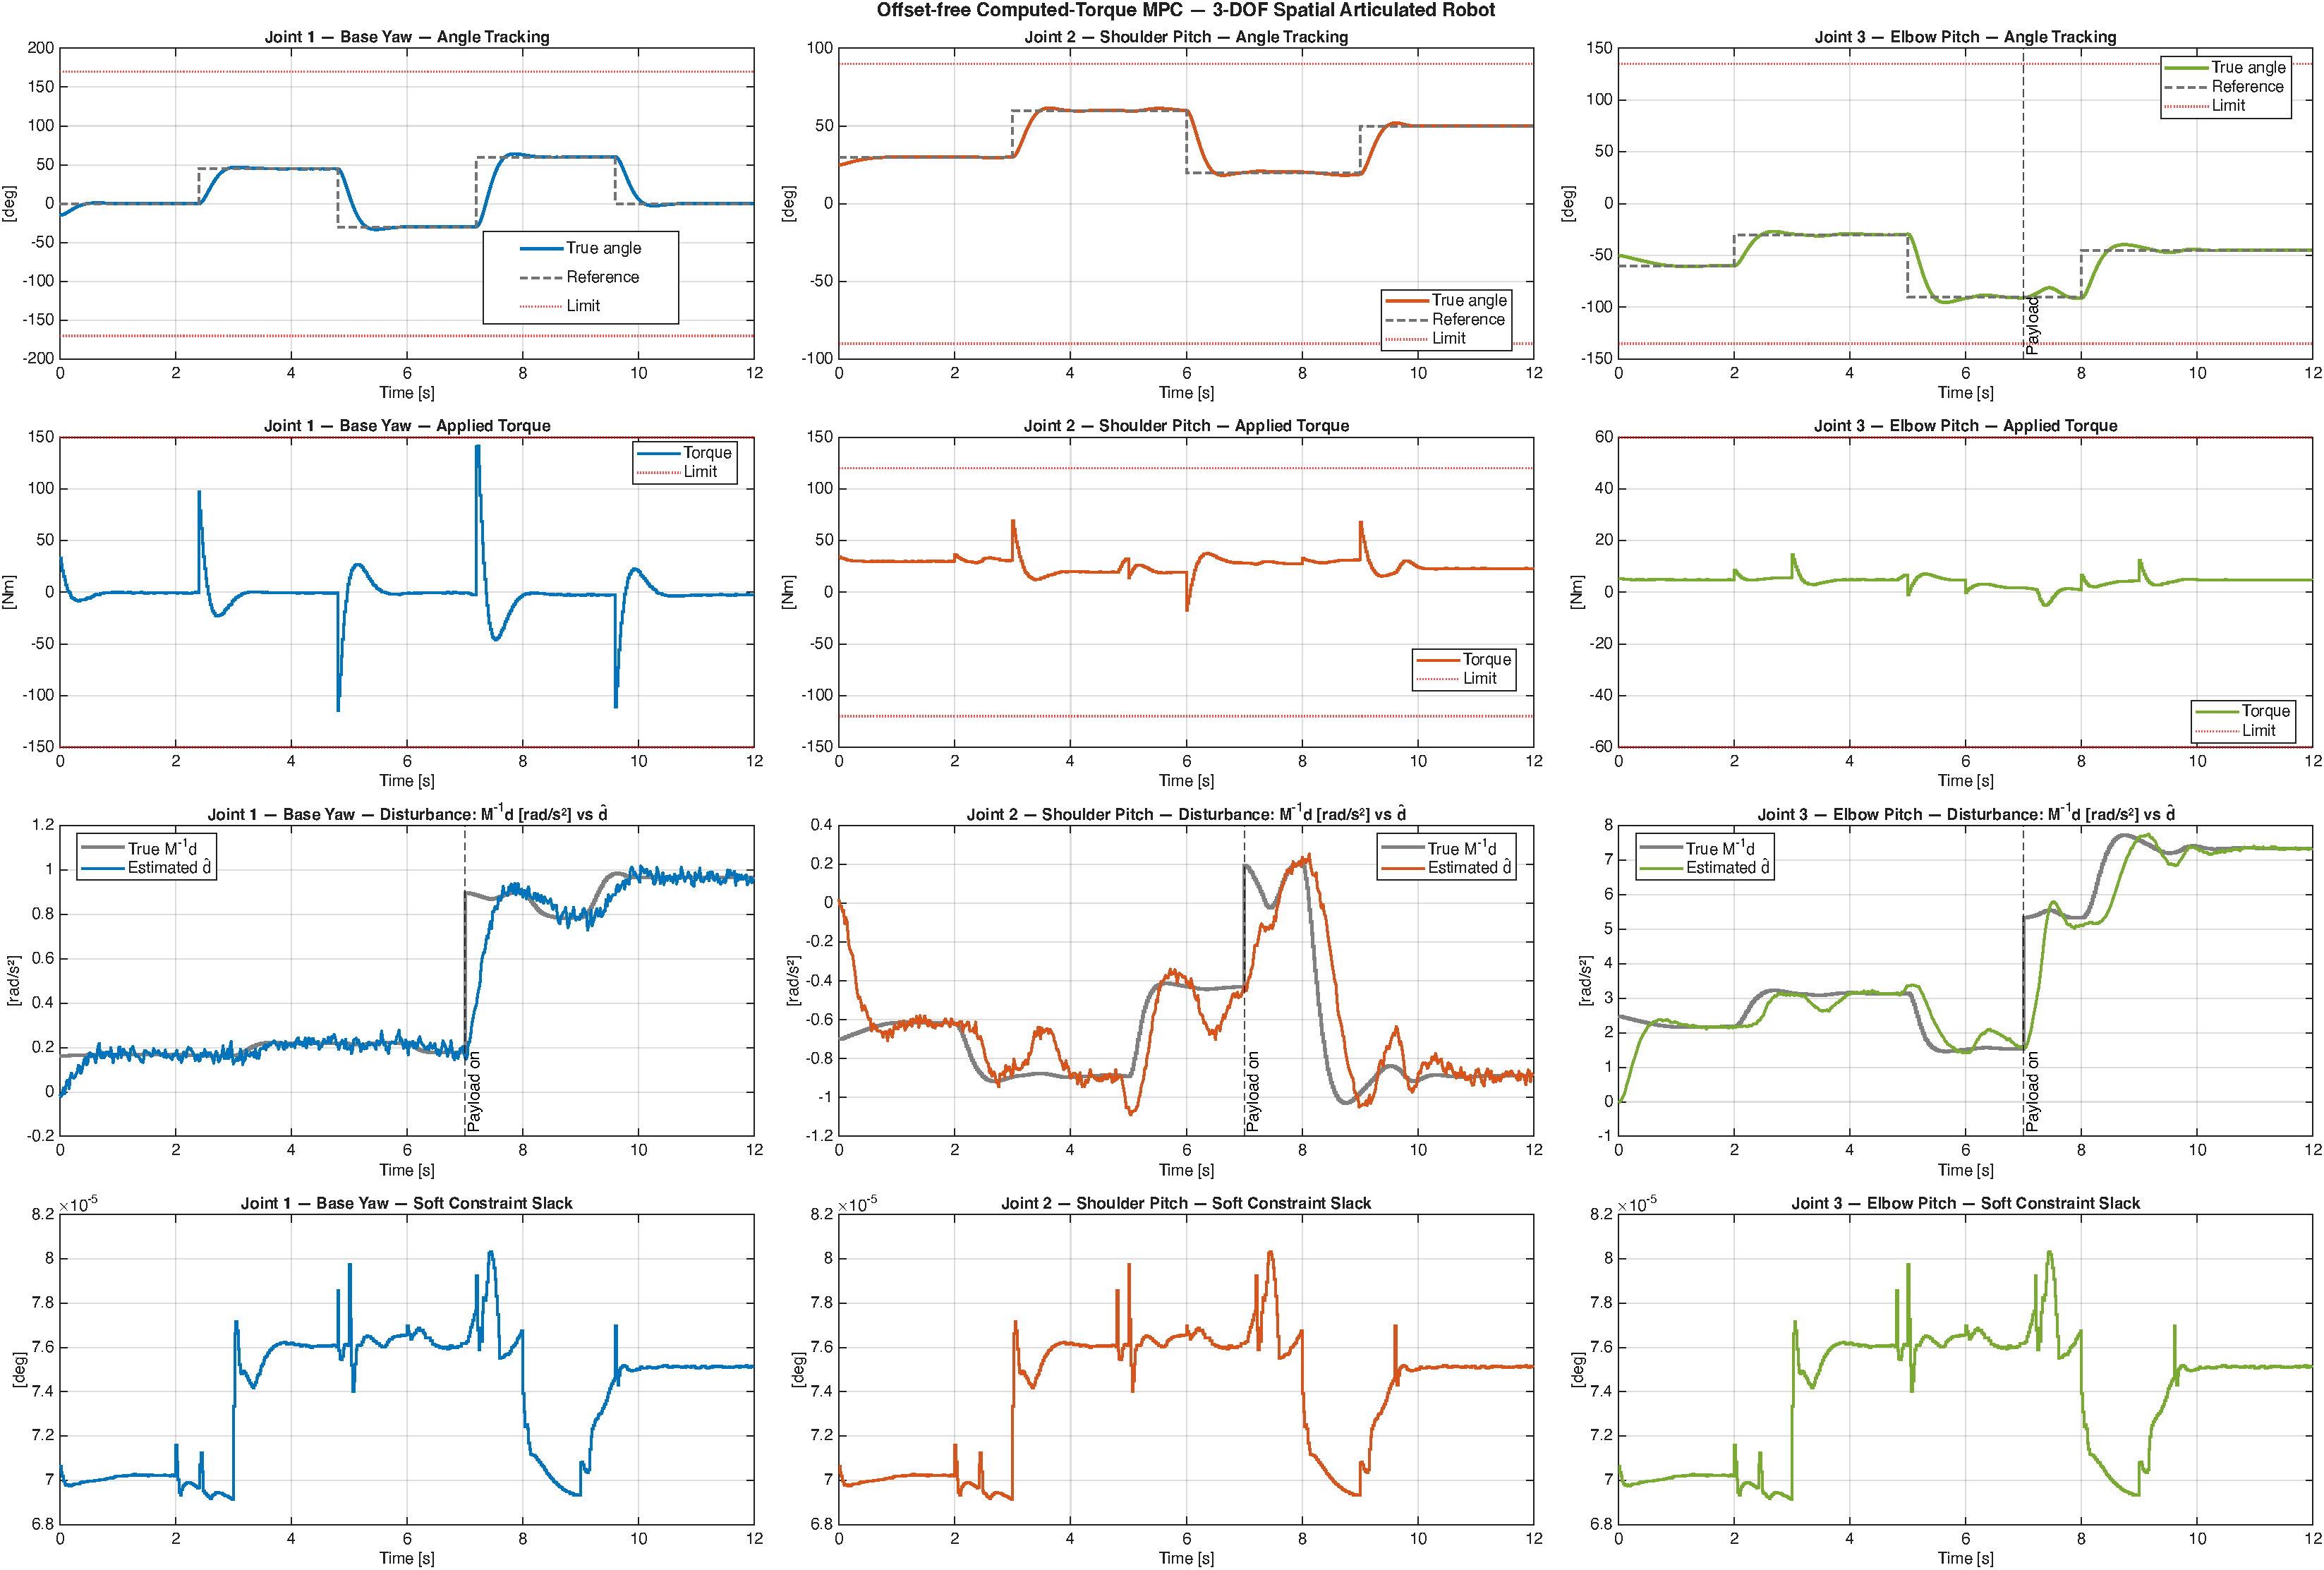
\includegraphics[width=1\linewidth]{Figures/Robot}
	    \captionof{figure}{Closed-loop performance of the offset-free computed-torque MPC applied to a 3-DOF spatial RRR articulated robot manipulator. The controller combines feedback linearisation (computed-torque law) with a deviation-form quadratic MPC ($N=15$, $T_s=20$\,ms) and an augmented Kalman filter for disturbance estimation. \textbf{Row~1}: Joint angle tracking for base yaw ($q_1$), shoulder pitch ($q_2$), and elbow pitch ($q_3$), with piecewise-constant reference trajectories (dashed) and joint limits (dotted red). \textbf{Row~2}: Applied actuator torques with saturation limits at $\pm150$, $\pm120$, and $\pm60$\,Nm, respectively. \textbf{Row~3}: Comparison of the true disturbance acceleration $M^{-1}(q)\,d$ (grey) and the Kalman filter estimate $\hat{d}$ (coloured), showing convergence after the payload step at $t=7$\,s. \textbf{Row~4}: Soft-constraint slack variables, which remain near zero throughout, confirming that joint limits are respected without significant violation. Constant friction biases ($0.5$, $-0.3$, $0.2$\,Nm) act on all joints from $t=0$, and an additional payload disturbance ($2.0$, $1.5$, $0.8$\,Nm) is applied at $t=7$\,s. The target calculator drives steady-state offsets to zero in all cases, demonstrating robust offset-free tracking despite unmodelled friction, sudden payload changes, and encoder noise ($\sigma=0.05^\circ$).}
	
		\label{fig:robot}


\end{examplebox}

\section*{Exercises}
\begin{enumerate}
	\item \textbf{Augmented State-Space Construction.}
	Consider a scalar plant
	\[
	x_{k+1} = 0.8\,x_k + u_k + d_k, \qquad y_k = x_k,
	\]
	where \(d_k\) is an unknown constant disturbance (\(d_{k+1}=d_k\)).
	\begin{enumerate}
		\item Define the augmented state vector \(z_k = [x_k,\; d_k]^T\) and write down the augmented system matrices \(A_{\mathrm{aug}}\), \(B_{\mathrm{aug}}\), and \(C_{\mathrm{aug}}\).
		\item Now suppose the disturbance enters only through the output, i.e.\ \(B_w = 0\) and \(C_d = 1\). How do the augmented matrices change?
		\item For the two-state system
		\[
		A = \begin{bmatrix} 1 & 0.1 \\ 0 & 0.95 \end{bmatrix}, \quad
		B = \begin{bmatrix} 0.005 \\ 0.1 \end{bmatrix}, \quad
		B_w = B, \quad
		C = \begin{bmatrix} 1 & 0 \end{bmatrix}, \quad C_d = 0,
		\]
		write out the full augmented matrices \(A_{\mathrm{aug}} \in \mathbb{R}^{3\times 3}\), \(B_{\mathrm{aug}} \in \mathbb{R}^{3\times 1}\), and \(C_{\mathrm{aug}} \in \mathbb{R}^{1\times 3}\).
	\end{enumerate}

	\item \textbf{Detectability of the Augmented System.}
	For the augmented pair \((A_{\mathrm{aug}},\, C_{\mathrm{aug}})\) constructed in Exercise~1(c):
	\begin{enumerate}
		\item Form the observability matrix
		\[
		\mathcal{O} = \begin{bmatrix} C_{\mathrm{aug}} \\ C_{\mathrm{aug}} A_{\mathrm{aug}} \\ C_{\mathrm{aug}} A_{\mathrm{aug}}^2 \end{bmatrix}
		\]
		and verify that its rank equals the dimension of the augmented state.
		\item Now suppose the system has two outputs \(y_k = C x_k\) with \(C = I_{2\times 2}\) and two independent disturbance states \(d_k \in \mathbb{R}^2\) with \(B_w = B\) and \(C_d = 0\). Does the augmented pair remain detectable? Justify your answer by examining the eigenvalues and the rank of the detectability test matrix \(\begin{bmatrix} A_{\mathrm{aug}} - \lambda I \\ C_{\mathrm{aug}} \end{bmatrix}\) at the eigenvalue \(\lambda = 1\).
		\item Explain the practical rule of thumb relating the number of disturbance states \(n_d\) to the number of measured outputs \(n_y\).
	\end{enumerate}

	\item \textbf{Steady-State Target Calculation.}
	Consider the system from Exercise~1(c) with the reference \(r_k = 2\) and a disturbance estimate \(\hat{d}_k = 0.5\).
	\begin{enumerate}
		\item Write out the target-calculator linear system
		\[
		\begin{bmatrix} I - A & -B \\ C & 0 \end{bmatrix}
		\begin{bmatrix} x_{ss} \\ u_{ss} \end{bmatrix}
		=
		\begin{bmatrix} B_w \hat{d}_k \\ r_k - C_d \hat{d}_k \end{bmatrix}
		\]
		with all numerical entries substituted.
		\item Solve for \(x_{ss}\) and \(u_{ss}\). Verify that the steady-state output satisfies \(C x_{ss} = r_k\).
		\item Suppose the input is constrained to \(-1 \le u \le 1\). Is the steady-state target \(u_{ss}\) feasible? If not, explain qualitatively how a constrained steady-state optimisation (as in Equation~\eqref{eq:target_qp}) would handle this situation.
	\end{enumerate}

	\item \textbf{Deviation-Form MPC Variables.}
	Using the targets \((x_{ss}, u_{ss})\) computed in Exercise~3:
	\begin{enumerate}
		\item Suppose the current state estimate is \(\hat{x}_k = [1.5,\; 0.3]^T\). Compute the initial deviation \(\tilde{x}_0 = \hat{x}_k - x_{ss}\).
		\item Write out the deviation-form prediction model \(\tilde{x}_{i+1} = A \tilde{x}_i + B \tilde{u}_i\) and explain why the disturbance estimate \(\hat{d}_k\) does not appear in this equation.
		\item If the hard input constraints are \(-1 \le u_k \le 1\), express these as constraints on the deviation input \(\tilde{u}_i\). Are the deviation-form constraints symmetric about zero?
		\item Explain the role of the terminal cost matrix \(P_{\mathrm{term}}\) in the MPC cost function~\eqref{eq:mpc_problem} and state how it is typically computed.
	\end{enumerate}

	\item \textbf{Effect of Misspecified \(B_w\).}
	Suppose the true plant has the disturbance entering through \(B_w^{\mathrm{true}} = [0;\; 1]\), but the augmented observer and target calculator are designed using the incorrect assumption \(B_w = B = [0.005;\; 0.1]\).
	\begin{enumerate}
		\item Will the augmented Kalman filter still converge to a constant disturbance estimate \(\hat{d}_k\) in steady state? Explain why or why not.
		\item At steady state, the target calculator enforces \((I-A)x_{ss} = B u_{ss} + B_w \hat{d}_k\) and \(C x_{ss} = r_k\). Does the controller still achieve zero steady-state output offset despite the mismatch in \(B_w\)? Argue from the structure of the equilibrium equations.
		\item Discuss the transient consequences of the misspecified \(B_w\). In particular, how might the transient response and the value of \(\hat{d}_k\) differ from the correctly specified case?
	\end{enumerate}

	\item \textbf{Comparison: MPC With and Without Disturbance Estimation.}
	Consider a standard (non-augmented) MPC regulator that uses the nominal model \(x_{k+1} = A x_k + B u_k\) without disturbance estimation, alongside the offset-free architecture of Algorithm~\ref{alg:offset_free_mpc}.
	\begin{enumerate}
		\item Suppose a constant disturbance \(d_k = d \neq 0\) acts on the plant through \(B_w\). Explain why the standard MPC regulator generally produces a non-zero steady-state tracking error. What is the source of the persistent offset?
		\item In the offset-free architecture, identify which component provides integral-action-like behaviour. How does the integrating disturbance model \(d_{k+1} = d_k\) relate to classical integral action?
		\item Suppose instead that the disturbance is sinusoidal, \(d_k = \sin(\omega k)\). Will the offset-free MPC with a constant disturbance model (\(d_{k+1} = d_k\)) eliminate the steady-state tracking error in this case? Justify your answer in terms of the internal model principle.
		\item Briefly outline how the disturbance model could be modified to handle the sinusoidal case.
	\end{enumerate}
\end{enumerate}

	% ============================================================
%  File: Chapter9.tex
%  \input this file as a chapter.
%  All environments reference the existing preamble; no extra
%  \usepackage or \definecolor declarations are needed.
% ============================================================

% ── Local TikZ styles ────────────────────────────────────────
\tikzset{
	slkblock/.style={
		rectangle, rounded corners=4pt,
		draw=blue!60!black, fill=blue!8,
		text width=#1, minimum height=1.0cm,
		align=center, font=\small\bfseries\sffamily
	},
	slkblock/.default=2.8cm,
	slkgreen/.style={slkblock=#1, draw=teal, fill=green!8},
	slkgreen/.default=2.8cm,
	slkred/.style={slkblock=#1, draw=red!70!black, fill=red!6},
	slkred/.default=2.8cm,
	slkyellow/.style={slkblock=#1, draw=yellow!60!black, fill=yellow!10},
	slkyellow/.default=2.8cm,
	slkarrow/.style={-Stealth, thick, draw=blue!60!black},
	slkdarrow/.style={-Stealth, thick, dashed, draw=red!60!black},
	siglabel/.style={font=\scriptsize\sffamily\itshape, midway},
	siglabelabove/.style={siglabel, above},
	siglabelbelow/.style={siglabel, below},
	siglabelright/.style={siglabel, right},
	siglabelleft/.style={siglabel, left},
}

% ============================================================
\chapter{Simulink Implementation of Model Predictive Control\texorpdfstring{$^{(*)}$}{(*)}}
\label{chap:simulink_mpc}
% ============================================================

% ─────────────────────────────────────────────────────────────
\section{General Implementation Guidance}
\label{sec:simulink_general}
% ─────────────────────────────────────────────────────────────

Simulink is widely used for rapid prototyping and hardware-in-the-loop
validation of control systems, and Model Predictive Control (MPC) is no
exception.  Implementing MPC in Simulink without the dedicated MPC
Toolbox requires a careful architectural decision: the optimisation
solver must be invoked at every simulation time step from within a
Simulink block, yet the solver itself — together with the YALMIP
modelling layer — relies on dynamic MATLAB features that are
incompatible with Simulink's default code-generation pipeline.  This
section establishes a general framework that resolves this tension.  The
approach is first described in fully general terms; Section~\ref{sec:simulink_building}
then applies it step by step to a concrete building temperature control
system.

% ─────────────────────────────────────────────────────────────
\subsection{Why the MPC Toolbox Is Not Required}
\label{subsec:no_toolbox}
% ─────────────────────────────────────────────────────────────

The MathWorks MPC Toolbox offers convenient pre-built blocks but
abstracts away the optimisation layer entirely.  This abstraction
becomes a limitation whenever the designer requires any of the
following:

\begin{itemize}[noitemsep]
	\item \textbf{Economic (non-regulatory) objectives} — for instance,
	minimising energy cost rather than a quadratic deviation from a
	setpoint;
	\item \textbf{Augmented observers} — such as Kalman filters that
	jointly estimate the plant state and an unmeasured disturbance;
	\item \textbf{Time-varying constraints} — comfort bands or
	operational limits that change according to a schedule;
	\item \textbf{Custom terminal costs or terminal sets} — required for
	rigorous closed-loop stability guarantees.
\end{itemize}

Using YALMIP together with \texttt{quadprog} or OSQP provides all of
this flexibility whilst keeping solver call-time well within a typical
sampling period.

% ─────────────────────────────────────────────────────────────
\subsection{The Code-Generation Barrier and How to Overcome It}
\label{subsec:extrinsic}
% ─────────────────────────────────────────────────────────────

MATLAB Function blocks in Simulink normally compile their contents into
C code at simulation start.  YALMIP relies on dynamic cell arrays,
runtime type inspection, and variable-argument function calls — none of
which survive compilation.  Attempting to call \texttt{sdpvar},
\texttt{optimizer}, or any YALMIP routine directly inside a compiled
block produces an immediate error.

The standard remedy is the \texttt{coder.extrinsic} declaration.  Any
function declared as extrinsic is \emph{not} compiled; instead, it
executes inside the full MATLAB interpreter at run time.  The
simulation still advances correctly — the block simply runs in
interpreted mode for the declared functions.

\begin{notebox}{Rules for \texttt{coder.extrinsic}}
	\begin{enumerate}[noitemsep]
		\item The declaration must appear at the \emph{top} of the MATLAB
		Function block body, before any use of the function.
		\item Every output variable must be \emph{pre-allocated} to a
		concrete type and size before the extrinsic call, so that
		Simulink can infer port dimensions at compile time.
		\item All YALMIP-dependent logic should live in a separate
		\texttt{.m} helper file; the block itself contains only the
		declaration and a single forwarding call.
	\end{enumerate}
	
	The general pattern inside any MATLAB Function block is:
	
	\begin{lstlisting}[language=Matlab]
		function y = MyBlock(u)
			coder.extrinsic('my_helper');   % declare before use
			y = zeros(size_of_output);      % pre-allocate
			y = my_helper(u);               % forward to helper
		end
	\end{lstlisting}
\end{notebox}

% ─────────────────────────────────────────────────────────────
\subsection{Managing State Across Time Steps: Persistent Variables}
\label{subsec:persistent}
% ─────────────────────────────────────────────────────────────

A Simulink MATLAB Function block does not retain values in its
workspace between consecutive invocations — each call begins with a
clean local scope.  An MPC controller, however, must preserve several
quantities across every time step:

\begin{itemize}[noitemsep]
	\item the observer state estimate $\hat{z}_k$;
	\item the last applied input $u_{k-1}$ (needed for the observer
	prediction step);
	\item any filtered disturbance estimates;
	\item the compiled YALMIP \texttt{optimizer} objects.
\end{itemize}

MATLAB's \texttt{persistent} keyword solves this problem.  A
persistent variable is initialised once on the first function call
and retains its value for the lifetime of the function in memory.
Within a Simulink simulation, this means the variable persists across
every time step from $k=1$ to the end of the run.

\begin{defnbox}{Persistent Variable Pattern for MPC Helper Functions}
	Declare all cross-step quantities with \texttt{persistent} at the
	top of the helper \texttt{.m} file, then guard initialisation with
	an \texttt{isempty} check:
	
	\begin{lstlisting}[language=Matlab]
		function u = my_mpc_step(y_meas, ...)
			persistent opt_obj observer_state u_prev
		
			if isempty(observer_state)           % runs on first call only
				opt_obj        = build_optimizers();
				observer_state = x0_guess;
				u_prev         = 0;
			end
		
			% ... rest of the control pipeline ...
		end
	\end{lstlisting}
	
	\textbf{Important:} before starting a new simulation run always
	execute \texttt{clear \textit{functionname}} in the MATLAB Command
	Window.  This resets all persistent variables to their initial
	state; failure to do so causes the controller to inherit the
	terminal conditions of the previous run.
\end{defnbox}

% ─────────────────────────────────────────────────────────────
\subsection{Building YALMIP Optimiser Objects: One-Time Compilation}
\label{subsec:build_general}
% ─────────────────────────────────────────────────────────────

YALMIP's \texttt{optimizer} function pre-processes the problem
structure — symbolic variable registration, sparsity analysis, and
conversion to the solver's native QP format — and returns a compiled
function handle.  This pre-processing is the expensive step (typically
10--30\,s for moderate-sized problems) and must not be repeated at
every simulation time step.

The correct approach is to create a dedicated initialisation function,
call it exactly once inside the persistent-variable guard shown above,
and store the resulting objects as persistent variables.  All
subsequent time steps call the compiled objects directly, which
typically completes in milliseconds.

\begin{lstlisting}[language=Matlab, caption={Skeleton of a one-time YALMIP initialisation function.}]
	function [opt1, opt2] = build_optimizers()
		% Called once. Returns compiled optimizer objects.
	
		% -- Define symbolic decision variables -----------------------
		x  = sdpvar(nx, 1);
		u  = sdpvar(nu, 1);
		p  = sdpvar(np, 1);    % parametric inputs (e.g. price, bounds)
	
		% -- Formulate constraints and objective ----------------------
		con = [ ... ];         % linear/quadratic constraints
		obj = ... ;            % quadratic cost
	
		% -- Compile with chosen solver -------------------------------
		ops  = sdpsettings('solver', 'quadprog', 'verbose', 0);
		opt1 = optimizer(con, obj, ops, {p}, {u});
	
		% -- Second optimizer (e.g. target calculator) ----------------
		% ...
	end
\end{lstlisting}

% ─────────────────────────────────────────────────────────────
\subsection{Recommended Architecture}
\label{subsec:architecture}
% ─────────────────────────────────────────────────────────────

The architecture that best reconciles Simulink's execution model with
YALMIP's requirements separates the design into two layers, as shown in
Figure~\ref{fig:architecture}.

\emph{Layer 1 — the Simulink canvas} contains only standard Simulink
blocks and thin MATLAB Function wrapper blocks.  Each wrapper declares
one helper function as extrinsic, pre-allocates its outputs, and
forwards its inputs.  Signal routing, the feedback connection, noise
injection, and input saturation are all handled by built-in Simulink
blocks.

\emph{Layer 2 — the helper \texttt{.m} files} contain all
computation: observer updates, YALMIP calls, QP solves, and persistent
state.  Because they execute in the full MATLAB interpreter they impose
no restrictions on the code they contain.

\begin{figure}[htbp]
	\centering
	\resizebox{\textwidth}{!}{%
		\begin{tikzpicture}[node distance=0.9cm and 3.2cm]
			
			%% ── Simulink layer: left column ──
			\node[slkyellow=3.4cm] (distgen)
			{Exogenous Signal\\Generator\\MATLAB Fn block};
			
			\node[slkblock=3.4cm, below=0.8cm of distgen] (plant)
			{Plant\\MATLAB Fn block};
			
			\node[slkblock=3.4cm, below=0.8cm of plant] (noise)
			{Measurement Noise\\{\scriptsize Sum + Random Number}};
			
			\node[slkblock=3.4cm, below=0.8cm of noise] (ctrl)
			{MPC Controller\\MATLAB Fn block};
			
			\node[slkblock=3.4cm, below=0.8cm of ctrl] (sat)
			{Saturation\\$[u_{\min},\;u_{\max}]$};
			
			%% ── Helper layer: right column ──
			\node[slkgreen=4.8cm, right=3.4cm of distgen] (hgen)
			{\texttt{signal\_generator.m}\\[2pt]
				{\small\normalfont Returns disturbances, references,\\
					and constraint parameters}};
			
			\node[slkgreen=4.8cm, right=3.4cm of plant] (hplant)
			{\texttt{plant\_model.m}\\[2pt]
				{\small\normalfont Discrete-time state update;\\
					persistent true state \texttt{x\_true}}};
			
			\node[slkgreen=4.8cm, right=3.4cm of ctrl] (hctrl)
			{\texttt{mpc\_step.m}\\[2pt]
				{\small\normalfont Observer update, target calculation,\\
					MPC QP solve; all persistent state}};
			
			\node[slkyellow=4.8cm, below=1.0cm of hctrl] (hbuild)
			{\texttt{build\_optimizers.m}\\[2pt]
				{\small\normalfont Builds YALMIP \texttt{optimizer} objects\\
					and observer gain; called once only}};
			
			%% ── Bounding boxes ──
			\begin{scope}[on background layer]
				\node[draw=blue!50, fill=blue!4, rounded corners=8pt,
				fit=(distgen)(plant)(noise)(ctrl)(sat),
				inner sep=12pt,
				label={[font=\small\bfseries\sffamily\color{blue!60!black}]
					above:{Layer 1 --- Simulink Canvas}}]
				(simbox) {};
			\end{scope}
			\begin{scope}[on background layer]
				\node[draw=teal, fill=green!4, rounded corners=8pt,
				fit=(hgen)(hplant)(hctrl)(hbuild),
				inner sep=12pt,
				label={[font=\small\bfseries\sffamily\color{teal}]
					above:{Layer 2 --- Helper \texttt{.m} Files (MATLAB Path)}}]
				(helperbox) {};
			\end{scope}
			
			%% ── Extrinsic call arrows ──
			\draw[slkarrow] (distgen.east) --
			node[siglabelabove]{\texttt{coder.extrinsic}} (hgen.west);
			\draw[slkarrow] (plant.east) --
			node[siglabelabove]{\texttt{coder.extrinsic}} (hplant.west);
			\draw[slkarrow] (ctrl.east) --
			node[siglabelabove]{\texttt{coder.extrinsic}} (hctrl.west);
			
			%% ── One-time build call (dashed) ──
			\draw[slkdarrow] (hctrl.south) --
			node[siglabelright, align=left]{called once\\(persistent guard)}
			(hbuild.north);
			
			%% ── Vertical signal flow within Simulink ──
			\draw[slkarrow] (distgen.south) --
			node[siglabelright]{$d_k$,\; known inputs} (plant.north);
			\draw[slkarrow] (plant.south) --
			node[siglabelright]{$y_\mathrm{true}$} (noise.north);
			\draw[slkarrow] (noise.south) --
			node[siglabelright]{$y_\mathrm{meas}$} (ctrl.north);
			\draw[slkarrow] (ctrl.south) --
			node[siglabelright]{$u_\mathrm{raw}$} (sat.north);
			
			%% ── Feedforward: exogenous signals to controller ──
			%% Four-leg orthogonal route: left → down → right → down into ctrl.west
			\coordinate (ffTurn)    at ($(distgen.west) + (-1.0, 0)$);
			\coordinate (ffApproach) at ($(ctrl.west)   + (-1.0, 0)$);
			
\draw[slkarrow]
(distgen.west)
-- (ffTurn)
-- (ffTurn |- ffApproach)
-- node[siglabelleft, align=left]{$r_k$\\exogenous inputs\\constraint parameters}
(ffApproach)
-- (ctrl.west);
			
			%% ── Feedback: Unit Delay ──
			\coordinate (fbTurn)   at ($(sat.west)  + (-1.8, 0)$);
			\coordinate (fbTarget) at ($(plant.west)+ (-1.8, 0)$);
			
			\draw[slkarrow]
			(sat.west)
			-- (fbTurn)                        % 1. left of sat
			-- (fbTarget)                      % 2. up alongside left edge
			-- node[siglabelabove]{$u_{k-1}$\; (Unit Delay)}
			([yshift=0pt]plant.west);       % 3. right into plant
			
		\end{tikzpicture}%
	}
	\caption{General two-layer architecture for Simulink-based MPC without the
		MPC Toolbox.  Layer~1 (Simulink canvas) contains only thin MATLAB Function
		wrapper blocks; all optimisation logic is delegated to Layer~2 helper files
		via \texttt{coder.extrinsic} calls.  Persistent variables in the helper files
		carry state across time steps and store the compiled \texttt{optimizer}
		objects for the lifetime of the simulation.}
	\label{fig:architecture}
\end{figure}

% ─────────────────────────────────────────────────────────────
\subsection{Eliminating the Algebraic Loop}
\label{subsec:algloop_general}
% ─────────────────────────────────────────────────────────────

In any discrete-time closed-loop Simulink model of the form
Plant~$\to$~Controller~$\to$~Plant, Simulink detects an
\emph{algebraic loop}: computing the plant output $y_k$ requires
the current input $u_k$, which itself requires $y_k$.  The standard
remedy is to insert a \emph{Unit Delay} block between the controller
output (or the saturation block) and the plant input:

\[
\cdots \to \text{Saturation} \;\xrightarrow{\;u_k\;}\;
\underbrace{\text{Unit Delay}}_{T_s,\;\mathrm{IC}=0}
\;\xrightarrow{\;u_{k-1}\;}\; \text{Plant} \to \cdots
\]

This is not an approximation — in a physically realisable digital
controller the input computed at step~$k$ cannot reach the actuator
until step~$k{+}1$.  The observer in the MPC helper file must
therefore use $u_{k-1}$ (stored as a persistent variable) rather than
$u_k$ in its prediction equation, which is achieved automatically by
the pattern shown in Section~\ref{subsec:persistent}.

% ─────────────────────────────────────────────────────────────
\subsection{Solver Recommendations}
\label{subsec:solvers}
% ─────────────────────────────────────────────────────────────

YALMIP supports a wide range of QP solvers through a common interface.
For typical MPC problems — moderate-horizon quadratic programmes with
linear constraints — the following two solvers are recommended.

\begin{center}
	\begin{tabular}{>{\bfseries\sffamily}l p{4.2cm} p{5.6cm}}
		\toprule
		Solver & Availability & Notes \\
		\midrule
		\texttt{quadprog} &
		Ships with MATLAB Optimisation Toolbox &
		Reliable, no warm-start across calls; sufficient for $N \leq 30$ \\[4pt]
		OSQP &
		Free, open-source; install via \texttt{osqp-matlab} &
		Supports warm-starting; recommended for long horizons or fast
		sampling rates \\
		\bottomrule
	\end{tabular}
\end{center}

Both are specified in YALMIP identically:
\begin{center}
\texttt{sdpsettings('solver','quadprog',...)} 
\end{center}


or
\begin{center}
\texttt{sdpsettings('solver','osqp',...)}.
\end{center}


% ─────────────────────────────────────────────────────────────
\subsection{Summary of the Implementation Workflow}
\label{subsec:workflow_summary}
% ─────────────────────────────────────────────────────────────

Figure~\ref{fig:workflow} summarises the complete development workflow.
The left column shows the \emph{offline} design steps that are
completed once before the Simulink model is built.  The right column
shows the \emph{runtime} sequence that executes automatically during
simulation.

\begin{figure}[htbp]
	\centering
	\resizebox{0.82\textwidth}{!}{%
		\begin{tikzpicture}[node distance=0.5cm]
			
			% ── OFFLINE column ──
			\node[slkblock=4.2cm] (d1) {Design discrete-time plant model \& choose $T_s$};
			\node[slkblock=4.2cm, below=0.5cm of d1] (d2) {Design observer\\(e.g.\ augmented Kalman filter)};
			\node[slkblock=4.2cm, below=0.5cm of d2] (d3) {Formulate YALMIP\\\texttt{optimizer} objects\\(cost, constraints, horizon)};
			\node[slkblock=4.2cm, below=0.5cm of d3] (d4) {Write helper \texttt{.m} files:\\
				\texttt{build\_optimizers.m},\\
				\texttt{plant\_model.m},\\
				\texttt{mpc\_step.m}, \ldots};
			\node[slkblock=4.2cm, below=0.5cm of d4] (d5) {Build Simulink model:\\
				add blocks, set solver to\\
				fixed-step discrete, $T_s$};
			
			\draw[slkarrow] (d1)--(d2); \draw[slkarrow] (d2)--(d3);
			\draw[slkarrow] (d3)--(d4); \draw[slkarrow] (d4)--(d5);
			
			\begin{scope}[on background layer]
				\node[draw=blue!50, fill=blue!4, rounded corners=6pt,
				fit=(d1)(d2)(d3)(d4)(d5), inner sep=10pt,
				label={[font=\small\bfseries\sffamily\color{blue!60!black}]
					above:Offline Design}] {};
			\end{scope}
			
			% ── RUNTIME column ──
			\node[slkgreen=4.2cm, right=2.8cm of d1] (r1)
			{\texttt{clear plant\_model}\\
				\texttt{clear mpc\_step}\\
				{\small(reset persistent vars)}};
			\node[slkgreen=4.2cm, below=0.5cm of r1] (r2)
			{Step $k=1$: \texttt{isempty} guard\\calls \texttt{build\_optimizers};\\
				YALMIP compiles QPs};
			\node[slkgreen=4.2cm, below=0.5cm of r2] (r3)
			{Steps $k \geq 2$:\\
				observer predict \& correct\\
				$\rightarrow$ target solve\\
				$\rightarrow$ MPC QP solve};
			\node[slkgreen=4.2cm, below=0.5cm of r3] (r4)
			{Apply $u_k$; Unit Delay\\feeds $u_{k-1}$ to plant\\at step $k{+}1$};
			\node[slkyellow=4.2cm, below=0.5cm of r4] (r5)
			{Simulation ends;\\ post-process logged signals};
			
			\draw[slkarrow] (r1)--(r2); \draw[slkarrow] (r2)--(r3);
			\draw[slkarrow] (r3)--(r4); \draw[slkarrow] (r4.east) -- ++(0.5,0) -- ++(0,1.5) -- node[siglabelright]{repeat $\forall k$} ++(-0.5,0)
			node[siglabelright]{repeat $\forall k$} (r3);
			\draw[slkarrow] (r4)--(r5);
			
			\begin{scope}[on background layer]
				\node[draw=teal, fill=green!4, rounded corners=6pt,
				fit=(r1)(r2)(r3)(r4)(r5), inner sep=10pt,
				label={[font=\small\bfseries\sffamily\color{teal}]
					above:Simulation Runtime}] {};
			\end{scope}
			
		\coordinate (mid) at ($(d5.east)!0.5!(r1.west)$);  % halfway horizontally
		
		\draw[slkarrow, ultra thick]
		(d5.east)
		-- (mid |- d5.east)                   % 1. right → midpoint, same height as d5
		-- (mid |- r1.west)                   % 2. up   → midpoint, same height as r1
		-- (r1.west)                          % 3. right → r1
		node[above, font=\small\sffamily, pos=0.5]{run};
			
		\end{tikzpicture}%
	}
	\caption{Complete Simulink MPC development and execution workflow.  The
		offline design phase (left) produces all \texttt{.m} helper files and
		the Simulink model.  On each new simulation run the persistent
		variables are cleared manually, after which the runtime sequence
		(right) executes automatically, compiling YALMIP objects once on the
		first step and solving the QP at every subsequent step.}
	\label{fig:workflow}
\end{figure}

% =============================================================

\section{Case Study: Single-Zone Building Heating}
\label{sec:simulink_building}
% =============================================================

We revisit the single-zone office heating problem introduced in the
previous chapter.  The general framework of
Section~\ref{sec:simulink_general} is now applied step by step to the
three-state physically derived RC model, combining an augmented Kalman
filter — which jointly estimates the three thermal states and an
unmeasured occupancy disturbance — with a two-layer economic MPC
comprising an economic steady-state target calculator and a
deviation-form MPC regulator with electricity-price preview.  This
example exercises every aspect of the general framework: persistent
optimiser objects, a multi-output profile generator, an extrinsic plant
block, and a feedback loop broken by a Unit Delay.

% -----------------------------------------------------------------
\subsection{System Description}
\label{subsec:system}
% -----------------------------------------------------------------

The discrete-time model of the single-zone building (sampling period
$T_s = 1800\,\mathrm{s}$, i.e.\ 30~min) is

\begin{equation*}
	x_{k+1} = A x_k + B u_k + E\,T_{\mathrm{amb},k}
	+ B_{\mathrm{sol}}\,\varphi_{\mathrm{sol},k}
	+ B_w\,d_k,
	\qquad
	y_k = C x_k + v_k,
\end{equation*}

\noindent where
$x_k = [T_{\mathrm{air},k},\; T_{w,\mathrm{in},k},\; T_{w,\mathrm{out},k}]^\top
\in \mathbb{R}^3$
contains indoor air temperature and the two wall-layer temperatures,
$u_k \in [0,\,2000]\,\mathrm{W}$ is heater power,
$T_{\mathrm{amb},k}$ and $\varphi_{\mathrm{sol},k}$ are the
\emph{measured} outdoor temperature and solar irradiance (known
feedforwards), and $d_k$ (${}^\circ$C/step) is the
\emph{unmeasured} occupancy-driven thermal disturbance.  The output

\[
y_k = 0.56\,T_{\mathrm{air},k} + 0.44\,T_{w,\mathrm{in},k}
\]

is the operative temperature (ISO~7726), measured with noise standard
deviation $\sigma_v = 0.1\,{}^\circ$C.

The pre-computed ZOH-discretised matrices are
\begin{multline*}
	A = \begin{bmatrix}
		0.8753 & 0.1102 & 0.0004 \\
		0.0275 & 0.9649 & 0.0073 \\
		0.0001 & 0.0049 & 0.9851
	\end{bmatrix}, \quad
	B = \begin{bmatrix}7.91\times10^{-4}\\1.00\times10^{-4}\\0\end{bmatrix},\quad
	E  = \begin{bmatrix}0.01404\\0.00025\\0.00993\end{bmatrix},\\[4pt]
	B_{\mathrm{sol}} = \begin{bmatrix}9.04\times10^{-6}\\1.43\times10^{-6}\\3.47\times10^{-4}\end{bmatrix}, \quad
	B_w = \begin{bmatrix}1.7647\\0.0267\\0\end{bmatrix},\quad
	C  = \begin{bmatrix}0.56 & 0.44 & 0\end{bmatrix}.
\end{multline*}

The control objective is to minimise electricity cost subject to
comfort constraints:
\[
y_{\min,k} \;\leq\; y_k \;\leq\; y_{\max,k},
\qquad
0 \;\leq\; u_k \;\leq\; 2000\,\mathrm{W},
\]
where the comfort bounds follow a daily occupancy schedule
($[20,\,23]\,{}^\circ$C during occupied hours 07:00--22:00,
$[15,\,26]\,{}^\circ$C overnight).

% -----------------------------------------------------------------
\subsection{File Structure}
\label{subsec:filestructure}
% -----------------------------------------------------------------

Following the general architecture of Section~\ref{subsec:architecture},
the implementation consists of four helper \texttt{.m} files and one
Simulink model file.  Table~\ref{tab:files} maps each file to the
corresponding generic role.

\begin{table}[htbp]
	\centering
	\caption{Helper files for the single-zone building case study and their
		correspondence to the general architecture.}
	\label{tab:files}
	\begin{tabular}{>{\ttfamily\small}l >{\small}l >{\small}p{5.2cm}}
		\toprule
		\normalfont\textbf{File} & \textbf{Generic role} & \textbf{Purpose} \\
		\midrule
		build\_mpc\_optimizers.m & \texttt{build\_optimizers.m} &
		Kalman gain (DARE), economic target \texttt{optimizer}, MPC regulator
		\texttt{optimizer} with price preview; called once \\[4pt]
		get\_profiles.m & \texttt{disturbance\_profiles.m} &
		Ambient temperature, solar irradiance, electricity price, current
		comfort bounds, and $N$-step future comfort bound vectors \\[4pt]
		plant\_step.m & \texttt{plant\_model.m} &
		One-step advance of the discrete RC building model; persistent
		true state \texttt{x\_true} and true occupancy disturbance \\[4pt]
		mpc\_controller\_step.m & \texttt{mpc\_step.m} &
		Kalman observer, economic target calculation, economic MPC QP
		solve with price preview; all state persistent \\[4pt]
		EconomicMPC.slx & Simulink model &
		Wires all wrapper blocks and standard blocks together \\
		\bottomrule
	\end{tabular}
\end{table}

All \texttt{.m} files and \texttt{EconomicMPC.slx} must reside in the
same folder, or all \texttt{.m} files must be accessible via
\texttt{addpath}.

% -----------------------------------------------------------------
\subsection{Step 1 — \texttt{build\_mpc\_optimizers.m}}
\label{subsec:build}
% -----------------------------------------------------------------

This function fulfils the role of the generic \texttt{build\_optimizers.m}
described in Section~\ref{subsec:build_general}.  It computes the
steady-state Kalman gain via \texttt{dare} and pre-compiles two YALMIP
\texttt{optimizer} objects: one for the economic steady-state target
and one for the deviation-form MPC regulator with $N$-step price
preview.  The compilation step runs exactly once, since the resulting
objects are stored as persistent variables in
\texttt{mpc\_controller\_step.m}.

\begin{lstlisting}[language=Matlab,
	caption={\texttt{build\_mpc\_optimizers.m} --- one-time initialisation
		function for the single-zone building controller.},
	label={lst:build}]
	function [target_calc, mpc_reg, L] = build_mpc_optimizers()
		% Builds YALMIP optimizer objects and the Kalman gain.
		% Called exactly once via the persistent guard in mpc_controller_step.m.
		fprintf('Building YALMIP optimizers -- please wait...\n');
		
		Ts = 1800;
		A     = [0.8753, 0.1102, 0.0004;
					0.0275, 0.9649, 0.0073;
					0.0001, 0.0049, 0.9851];
		B     = [7.91e-4; 1.00e-4; 0      ];
		E     = [0.01404; 0.00025; 0.00993];
		Bsol  = [9.04e-6; 1.43e-6; 3.47e-4];
		Bw    = [1.7647;  0.0267;  0      ];
		C     =  [0.56, 0.44, 0];
		nx = 3;  nu = 1;  u_min = 0;  u_max = 2000;
		
		%% -- Augmented Kalman filter (state + occupancy disturbance) ------
		%    z = [x; d],  random-walk disturbance model
		A_aug   = [A, Bw; zeros(1,nx), 1];
		B_aug   = [B; 0];
		E_aug   = [E; 0];
		Bsol_aug= [Bsol; 0];
		C_aug   = [C, 0];
		
		W_kf = diag([1e-3, 1e-3, 1e-3, (0.01)^2]);  % sqrt(W_d)=0.01 degC/step
		V_kf = 0.1^2;
		[P_kf,~,~] = dare(A_aug', C_aug', W_kf, V_kf);
		L = P_kf * C_aug' / (C_aug * P_kf * C_aug' + V_kf);
		
		%% -- Economic steady-state target optimizer -----------------------
		price_k  = sdpvar(1,1);  d_hat_k  = sdpvar(1,1);
		T_amb_k  = sdpvar(1,1);  phi_k    = sdpvar(1,1);
		y_min_k  = sdpvar(1,1);  y_max_k  = sdpvar(1,1);
		xs = sdpvar(nx,1);  us = sdpvar(nu,1);  ss_slack = sdpvar(1,1);
		
		ss_cons = [xs == A*xs + B*us + E*T_amb_k + Bsol*phi_k + Bw*d_hat_k, ...
		y_min_k - ss_slack <= C*xs <= y_max_k + ss_slack, ...
		u_min <= us <= u_max,  ss_slack >= 0];
		ss_obj  = price_k * us + 1e4 * ss_slack^2;
		
		ops_ss      = sdpsettings('solver','quadprog','verbose',0);
		target_calc = optimizer(ss_cons, ss_obj, ops_ss, ...
		{price_k, d_hat_k, T_amb_k, phi_k, y_min_k, y_max_k}, ...
		[xs; us]);
		
		%% -- Economic MPC regulator with N-step price preview -------------
		%    Stage cost: ||x_tilde||_Q^2 + beta*price*u*(Ts/3600) + rho*slack^2
		%    Penalty hierarchy: rho >> beta*p_max*u_max*(Ts/3600)
		%    i.e.  1e7 >> 6*0.28*2000*0.5 = 1680
		N = 24;  Q = diag([5,2,1]);  beta = 6;  rho = 1e7;
		[P_term,~,~] = dare(A, B, Q, 1e-3);
		
		du_v     = sdpvar(nu,N,'full');    dx_v  = sdpvar(nx,N+1,'full');
		slk      = sdpvar(1,N,'full');
		xh_v     = sdpvar(nx,1);   xs_v = sdpvar(nx,1);  us_v = sdpvar(nu,1);
		Ymn      = sdpvar(1,N,'full');     Ymx   = sdpvar(1,N,'full');
		Price_v  = sdpvar(1,N,'full');
		
		obj = 0;
		con = [dx_v(:,1) == xh_v - xs_v];
		for i = 1:N
			u_abs = du_v(:,i) + us_v;
			x_pred_i = dx_v(:,i+1) + xs_v;
			con = [con, ...
			dx_v(:,i+1) == A*dx_v(:,i) + B*du_v(:,i), ...
			u_min <= u_abs <= u_max, ...
			Ymn(i)-slk(i) <= C*x_pred_i <= Ymx(i)+slk(i), slk(i) >= 0];
			obj = obj + dx_v(:,i)'*Q*dx_v(:,i) ...
			+ beta*Price_v(i)*u_abs*(Ts/3600) ...
			+ rho*slk(i)^2;
		end
		obj = obj + dx_v(:,N+1)' * P_term * dx_v(:,N+1);
		
		ops_mpc = sdpsettings('solver','quadprog','verbose',0);
		mpc_reg = optimizer(con, obj, ops_mpc, ...
		{xh_v, xs_v, us_v, Ymn, Ymx, Price_v}, du_v(:,1));
		
		fprintf('Optimizers ready.\n');
	end
\end{lstlisting}

\begin{notebox}{Horizon and Tuning Parameters}
	The prediction horizon $N = 24$ steps corresponds to 12\,hours at
	$T_s = 30\,\mathrm{min}$, allowing the controller to anticipate the
	morning and evening price transitions.  The state penalty
	$Q = \mathrm{diag}(5,2,1)$ weights the air temperature most heavily.
	The economic weight $\beta = 6$ and the comfort slack penalty
	$\rho = 10^7$ satisfy the hierarchy $\rho \gg
	\beta\,p_{\max}\,u_{\max}\,(T_s/3600) = 1680$, guaranteeing that
	comfort violations are never preferred over heating.  The terminal
	cost $P_\infty$ is the DARE solution, ensuring asymptotic stability
	of the unconstrained closed-loop.
\end{notebox}

% -----------------------------------------------------------------
\subsection{Step 2 — \texttt{get\_profiles.m}}
\label{subsec:profiles}
% -----------------------------------------------------------------

This function fulfils the role of the generic
\texttt{disturbance\_profiles.m}.  It receives the current simulation
time in seconds from the Simulink \textit{Clock} block and returns all
time-varying exogenous signals: ambient temperature, solar irradiance,
electricity price, current comfort bounds, and the $N$-step future
comfort bound and price vectors required by the MPC optimiser.

\begin{lstlisting}[language=Matlab,
	caption={\texttt{get\_profiles.m} --- provides current and forecast
		exogenous signals for the MPC horizon (48-hour winter scenario).},
	label={lst:profiles}]
	function [T_amb, Solar, Price, Tmin, Tmax, Tmin_fut, Tmax_fut, Price_fut] = ...
	get_profiles(t)
		% Input:  t in seconds (Simulink Clock output).
		% Outputs: scalars for current step + 1x24 vectors for MPC horizon.
		N  = 24;  Ts = 1800;  t_h = t / 3600;
		
		% Outdoor temperature: nominally -1 to 11 degC (winter scenario)
		T_amb = 5 + 6*sin(2*pi*(t_h - 14)/24) + 0.5*randn;
		
		% Solar irradiance: daytime half-sine, zero at night
		Solar = max(0, 600*sin(pi*(mod(t_h,24) - 8)/9));
		
		% Electricity price: peak / off-peak tariff
		is_peak = (mod(t_h,24) >= 7) && (mod(t_h,24) < 22);
		if is_peak
			Price = 0.28;  Tmin = 20;  Tmax = 23;
		else
			Price = 0.05;  Tmin = 15;  Tmax = 26;
		end
		
		% N-step future comfort bounds and price sequence for MPC
		Tmin_fut  = zeros(1,N);  Tmax_fut  = zeros(1,N);
		Price_fut = zeros(1,N);
		for i = 1:N
			t_fut = t_h + i*(Ts/3600);
			if (mod(t_fut,24) >= 7) && (mod(t_fut,24) < 22)
				Tmin_fut(i)  = 20;   Tmax_fut(i)  = 23;
				Price_fut(i) = 0.28;
			else
				Tmin_fut(i)  = 15;   Tmax_fut(i)  = 26;
				Price_fut(i) = 0.05;
			end
		end
	end
\end{lstlisting}

% -----------------------------------------------------------------
\subsection{Step 3 — \texttt{plant\_step.m}}
\label{subsec:plant}
% -----------------------------------------------------------------

This function fulfils the generic \texttt{plant\_model.m} role.  The
true state $x_\mathrm{true}$ is stored as a persistent variable.  On
each call the function returns the current measured operative
temperature $y_\mathrm{true} = C x_\mathrm{true}$ and then advances
the state by one step, incorporating the heater input, solar irradiance,
ambient temperature, and the true occupancy disturbance (unknown to the
controller).

\begin{lstlisting}[language=Matlab,
	caption={\texttt{plant\_step.m} --- discrete 3-state RC building model
		with persistent true state and true occupancy disturbance.},
	label={lst:plant}]
	function y_true = plant_step(u, T_amb, Solar, t)
		% Run  clear plant_step  before each new simulation.
		% t: current time in seconds (used to compute true occupancy).
		persistent x_true
		A    = [0.8753, 0.1102, 0.0004;
					0.0275, 0.9649, 0.0073;
					0.0001, 0.0049, 0.9851];
		B    = [7.91e-4; 1.00e-4; 0      ];
		E    = [0.01404; 0.00025; 0.00993];
		Bsol = [9.04e-6; 1.43e-6; 3.47e-4];
		Bw   = [1.7647;  0.0267;  0      ];
		C    = [0.56, 0.44, 0];
		
		if isempty(x_true)
			x_true = [19; 17; 10];  % initial temperatures: air, inner wall, outer wall
		end
		
		% True occupancy: 300 W internal gains => 0.191 degC/step
		t_h   = t / 3600;
		d_occ = 0.191 * double(mod(t_h,24) >= 8 && mod(t_h,24) < 18);
		
		y_true = C * x_true;
		x_true = A*x_true + B*u + E*T_amb + Bsol*Solar + Bw*d_occ;
	end
\end{lstlisting}

% -----------------------------------------------------------------
\subsection{Step 4 — \texttt{mpc\_controller\_step.m}}
\label{subsec:controller}
% -----------------------------------------------------------------

This is the main control file, fulfilling the role of the generic
\texttt{mpc\_step.m}.  It implements the persistent-variable pattern
described in Section~\ref{subsec:persistent}: on the first call it
invokes \texttt{build\_mpc\_optimizers} and initialises the augmented
Kalman state; on every subsequent call it executes the three-stage
pipeline shown in Figure~\ref{fig:control_pipeline}.

\begin{figure}[htbp]
	\centering
	\resizebox{\textwidth}{!}{%
		\begin{tikzpicture}[node distance=0.6cm and 1.8cm]
			
			%% -- Stage nodes --
			\node[slkgreen=3.6cm] (obs)
			{Stage 1\\[2pt]\textbf{Kalman Observer}\\{\scriptsize predict $+$ correct}};
			
			\node[slkblock=3.6cm, right=1.8cm of obs] (tgt)
			{Stage 2\\[2pt]\textbf{Target Calculator}\\{\scriptsize economic SS optimum}};
			
			\node[slkred=3.6cm, right=1.8cm of tgt] (mpc)
			{Stage 3\\[2pt]\textbf{MPC Regulator}\\{\scriptsize deviation-form QP}};
			
			\node[slkyellow=2cm, right=1.4cm of mpc] (sat)
			{\textbf{Saturate}\\$[0,\;2000]$};
			
			%% -- Input / output labels --
			\node[left=1.1cm of obs, align=right, font=\small\sffamily] (inputs)
			{$y_\mathrm{meas}$\\$T_\mathrm{amb}$\\$\varphi_\mathrm{sol}$\\
				price\\$\underline{y},\bar{y}$};
			
			\node[right=0.7cm of sat, align=left, font=\small\sffamily] (output)
			{$u_k$};
			
			%% -- Main pipeline arrows --
			\draw[slkarrow] (inputs.east) -- (obs.west);
			\draw[slkarrow] (obs.east)  -- node[siglabelabove]{$\hat{x}_k$, $\hat{d}_k$} (tgt.west);
			\draw[slkarrow] (tgt.east)  -- node[siglabelabove]{$x^\mathrm{s}_k$, $u^\mathrm{s}_k$} (mpc.west);
			\draw[slkarrow] (mpc.east)  -- node[siglabelabove]{$u^\mathrm{s}_k + \delta u^*$} (sat.west);
			\draw[slkarrow] (sat.east)  -- (output.west);
			
			%% -- Persistent box --
			\begin{scope}[on background layer]
				\node[draw=teal, fill=green!4, rounded corners=6pt,
				fit=(obs)(tgt)(mpc), inner sep=8pt,
				label={[font=\small\bfseries\sffamily\color{teal}]
					below:Persistent: \texttt{z\_est}, \texttt{u\_prev},
					\texttt{target\_calc}, \texttt{mpc\_reg}, \texttt{L}}]
				(persistbox) {};
			\end{scope}
			
			%% -- Future bounds and prices: orthogonal routing --
			\coordinate (rail-left)  at ($(inputs.south) + (0, -1.75)$);
			\coordinate (rail-right) at ($(mpc.south)    + (0, -2.2)$);
			
			\draw[slkdarrow]
			(inputs.south)
			-- (rail-left)
			-- node[below, font=\small\sffamily\itshape]
			{$\underline{y}_{k+1:k+N},\;\overline{y}_{k+1:k+N},\;
				p_{k+1:k+N}$}
			(rail-right)
			-- (mpc.south);
			
		\end{tikzpicture}%
	}
	\caption{Three-stage control pipeline executed at every sampling instant
		inside \texttt{mpc\_controller\_step.m}.  The dashed arrow carries the
		$N$-step future comfort bounds \emph{and} electricity-price sequence
		directly from the input port to the MPC Regulator, bypassing the
		observer and target stages.  All persistent quantities are retained
		between calls via MATLAB's \texttt{persistent} keyword.}
	\label{fig:control_pipeline}
\end{figure}

\begin{lstlisting}[language=Matlab,
	caption={\texttt{mpc\_controller\_step.m} --- complete economic
		offset-free MPC pipeline following the general pattern of
		Section~\ref{subsec:persistent}.},
	label={lst:controller}]
	function u = mpc_controller_step(y_meas, T_amb, Solar, Price, ...
	Tmin, Tmax, Tmin_fut, Tmax_fut, Price_fut)
		% Full Economic MPC step: observer -> target -> MPC.
		% Run  clear mpc_controller_step  before each new simulation.
		
		persistent target_calc mpc_reg L z_est u_prev
		
		Ts = 1800;
		A_aug   = [ 0.8753, 0.1102, 0.0004, 1.7647;
							0.0275, 0.9649, 0.0073, 0.0267;
							0.0001, 0.0049, 0.9851, 0.0000;
							0,      0,      0,      1     ];
		B_aug   = [7.91e-4; 1.00e-4; 0; 0];
		E_aug   = [0.01404; 0.00025; 0.00993; 0];
		Bsol_aug= [9.04e-6; 1.43e-6; 3.47e-4; 0];
		C_aug   = [0.56, 0.44, 0, 0];
		nx = 3;  u_min = 0;  u_max = 2000;
		
		%% -- First call: initialise (Section 9.1.3 pattern) ---------------
		if isempty(z_est)
			[target_calc, mpc_reg, L] = build_mpc_optimizers();
			z_est  = [19; 17; 10; 0];  % [T_air; T_w_in; T_w_out; d_hat]
			u_prev = 0;
		end
		
		%% -- Stage 1: Kalman observer (predict + correct) -----------------
		z_pred = A_aug*z_est + B_aug*u_prev + E_aug*T_amb + Bsol_aug*Solar;
		z_est  = z_pred + L*(y_meas - C_aug*z_pred);
		x_hat  = z_est(1:nx);
		d_hat  = z_est(end);
		
		%% -- Stage 2: Economic steady-state target ------------------------
		[ss_sol, flag_ss] = target_calc{Price, d_hat, T_amb, Solar, Tmin, Tmax};
		if flag_ss ~= 0
			warning('Target calculator failed -- applying fallback.');
			x_ss = x_hat;  u_ss = u_prev;
		else
			ss_sol = full(ss_sol);
			x_ss   = ss_sol(1:nx);
			u_ss   = ss_sol(nx+1);
		end
		
		%% -- Stage 3: Economic MPC regulator (deviation form) -------------
		[du, flag_mpc] = mpc_reg{x_hat, x_ss, u_ss, Tmin_fut, Tmax_fut, Price_fut};
		if flag_mpc ~= 0
			warning('MPC regulator failed -- applying steady-state input.');
			du = 0;
		else
			du = full(du);
		end
		
		%% -- Saturate and store -------------------------------------------
		u      = min(max(u_ss + du, u_min), u_max);
		u_prev = u;
	end
\end{lstlisting}

% -----------------------------------------------------------------
\subsection{Step 5 — Building the Simulink Model}
\label{subsec:slx}
% -----------------------------------------------------------------

With all four helper files in place, the Simulink model requires only
standard block types and three MATLAB Function wrapper blocks.  The
complete signal flow is shown in Figure~\ref{fig:simulink_flow}.

\subsubsection{Solver Configuration}

Open the \textit{Configuration Parameters} dialogue (\texttt{Ctrl+E})
and apply the settings in Table~\ref{tab:solver}.  Selecting the
discrete (no continuous states) solver is essential because all
dynamics are managed inside the helper files via persistent variables.

\begin{table}[htbp]
	\centering
	\caption{Simulink solver configuration for the single-zone building
		temperature control model.}
	\label{tab:solver}
	\begin{tabular}{lll}
		\toprule
		\textbf{Parameter} & \textbf{Value} & \textbf{Reason} \\
		\midrule
		Stop time       & \texttt{172800}  & 48\,h $\times$ 3600\,s/h \\
		Solver type     & Fixed-step       & Discrete controller \\
		Solver          & \texttt{discrete (no continuous states)} & States in persistent vars \\
		Fixed-step size & \texttt{1800}    & $T_s = 30\,\mathrm{min}$ \\
		\bottomrule
	\end{tabular}
\end{table}

\subsubsection{Block Placement and Wrapper Code}

Table~\ref{tab:blocks} lists every block in the model.  Each of the
three MATLAB Function blocks must contain the corresponding wrapper
from Listing~\ref{lst:wrapper}.

\begin{table}[!htbp]
	\centering
	\caption{Simulink blocks required for the single-zone building
		temperature control model.}
	\label{tab:blocks}
	\begin{tabular}{>{\ttfamily\small}l >{\small}l >{\small}p{5.5cm}}
		\toprule
		\normalfont\textbf{Label} & \textbf{Library path} & \textbf{Key parameter} \\
		\midrule
		Clock       & Sources $>$ Clock                           & Decimation: 1 \\
		ProfileGen  & User-Defined Functions $>$ MATLAB Function  & Wrapper: Listing~\ref{lst:wrapper} \\
		Plant       & User-Defined Functions $>$ MATLAB Function  & Wrapper: Listing~\ref{lst:wrapper} \\
		AddNoise    & Math Operations $>$ Sum                     & Signs: \texttt{++} \\
		MeasNoise   & Sources $>$ Random Number                   & Mean: 0, Var: 0.01, $T_s$: 1800 \\
		UnitDelay   & Discrete $>$ Unit Delay                     & $T_s$: 1800, IC: 0 \\
		Controller  & User-Defined Functions $>$ MATLAB Function  & Wrapper: Listing~\ref{lst:wrapper} \\
		Saturation  & Discontinuities $>$ Saturation              & Lower: 0, Upper: 2000 \\
		ToWorkspace & Sinks $>$ To Workspace                      & One block per logged signal \\
		\bottomrule
	\end{tabular}
\end{table}

\begin{lstlisting}[language=Matlab,
	caption={Wrapper code for the three MATLAB Function blocks.  Each
		wrapper pre-allocates its outputs, declares the helper as
		extrinsic, and forwards its inputs --- following the pattern
		of Section~\ref{subsec:extrinsic}.},
	label={lst:wrapper}]
	%% ---- ProfileGen block ------------------------------------------
	function [T_amb, Solar, Price, Tmin, Tmax, Tmin_fut, Tmax_fut, Price_fut] = ...
	ProfileGen(t)
		coder.extrinsic('get_profiles');
		T_amb = 0;  Solar = 0;  Price = 0;  Tmin = 0;  Tmax = 0;
		Tmin_fut  = zeros(1,24);  Tmax_fut  = zeros(1,24);
		Price_fut = zeros(1,24);
		[T_amb, Solar, Price, Tmin, Tmax, Tmin_fut, Tmax_fut, Price_fut] = ...
		get_profiles(t);
	end
	
	%% ---- Plant block -----------------------------------------------
	function y_true = Plant(u, T_amb, Solar, t)
		coder.extrinsic('plant_step');
		y_true = 0;
		y_true = plant_step(u, T_amb, Solar, t);
	end
	
	%% ---- Controller block -----------------------------------------
	function u = Controller(y_meas, T_amb, Solar, Price, ...
		Tmin, Tmax, Tmin_fut, Tmax_fut, Price_fut)
		coder.extrinsic('mpc_controller_step');
		u = 0;
		u = mpc_controller_step(y_meas, T_amb, Solar, Price, ...
		Tmin, Tmax, Tmin_fut, Tmax_fut, Price_fut);
	end
\end{lstlisting}

\begin{figure}[htbp]
	\centering
	\resizebox{\textwidth}{!}{%
		\begin{tikzpicture}[node distance=0.6cm and 0.55cm]
			
			%% -- Top row --
			\node[slkyellow=1.2cm] (clock) {Clock\\$t$};
			
			\node[slkgreen=2.6cm, right=0.7cm of clock] (prof)
			{Profile\\Generator\\{\scriptsize\ttfamily get\_profiles}};
			
			%% -- Main row --
			\node[slkblock=2.2cm, below=2.4cm of prof] (plant)
			{Plant\\{\scriptsize\ttfamily plant\_step}};
			
			\node[slkblock=1.6cm, right=0.7cm of plant] (sum)
			{Sum\\$++$};
			
			\node[slkyellow=1.8cm, below=0.7cm of sum] (noise)
			{Random\\Number\\{\scriptsize $\mathcal{N}(0,0.01)$}};
			
			\node[slkred=3.0cm, right=0.9cm of sum] (ctrl)
			{Controller\\{\scriptsize\ttfamily mpc\_controller\_step}};
			
			\node[slkblock=1.8cm, right=0.8cm of ctrl] (sat)
			{Saturation\\$[0,\;2000]$};
			
			\node[slkyellow=1.8cm, right=0.7cm of sat] (delay)
			{Unit\\Delay\\$T_s=1800$};
			
			%% -- Tap points --
			\coordinate (tapYmeas) at ($(sum.east)!0.5!(ctrl.west)$);
			\coordinate (tapU)     at ($(sat.east)!0.5!(delay.west)$);
			
			%% -- To Workspace blocks --
			\node[slkyellow=1.8cm, above=2.2cm of tapYmeas] (tw1)
			{To Workspace\\$y_\mathrm{meas}$};
			\node[slkyellow=1.8cm, above=2.2cm of tapU] (tw2)
			{To Workspace\\$u_k$};
			
			%% -- Signal wiring --
			\draw[slkarrow] (clock.east) --
			node[siglabelabove]{$t$} (prof.west);
			
			\draw[slkarrow] (prof.south) -- ++(0,-0.4) -|
			node[siglabelleft, pos=0.15]{$T_\mathrm{amb}$, $\varphi_\mathrm{sol}$}
			(plant.north);
			
			\draw[slkarrow] (plant.east) --
			node[siglabelabove]{$y_\mathrm{true}$} (sum.west);
			
			\draw[slkarrow] (noise.north) -- (sum.south);
			
			\draw[slkarrow] (sum.east) --
			node[siglabelabove]{$y_\mathrm{meas}$} (ctrl.west);
			
			\draw[slkdarrow] (tapYmeas) -- (tw1.south);
			
			%% ProfileGen -> Controller detour
			\coordinate (profTurn)     at ($(prof.east)   + (0.6, 0)$);
			\coordinate (ctrlApproach) at ($(ctrl.north)  + (0,   0.5)$);
			
			\draw[slkarrow]
			(prof.east)
			-- (profTurn)
			-- (profTurn |- ctrlApproach)
			-- node[siglabelleft]
			{price, $T_\mathrm{amb}$, $\varphi_\mathrm{sol}$,
				$\underline{y}$, $\overline{y}$, futures}
			(ctrlApproach)
			-- (ctrl.north);
			
			\draw[slkarrow] (ctrl.east) --
			node[siglabelabove]{$u_\mathrm{raw}$} (sat.west);
			
			\draw[slkarrow] (sat.east) --
			node[siglabelabove]{$u_k$} (delay.west);
			
			\draw[slkdarrow] (tapU) -- (tw2.south);
			
			%% Feedback loop (u_{k-1} -> plant and -> controller via clock)
			\draw[slkarrow] (delay.south) -- ++(0,-2.6) -|
			node[siglabelbelow, pos=0.15]{$u_{k-1}$}
			(plant.south);
			
			\draw[slkarrow] (clock.south) |-
			node[siglabelbelow, pos=0.75]{$t$}
			(plant.west);
			
			%% -- Bounding box --
			\coordinate (feedbot) at ($(delay.south) + (0,-3.2)$);
			\begin{scope}[on background layer]
				\node[draw=blue!40, fill=blue!3, rounded corners=6pt,
				fit=(clock)(prof)(plant)(sum)(noise)
				(ctrl)(sat)(delay)(tw1)(tw2)(feedbot),
				inner sep=10pt] {};
			\end{scope}
			
		\end{tikzpicture}%
	}
	\caption{Complete conceptual Simulink signal flow for the single-zone
		building economic MPC\@.  The Clock output $t$ is passed both to the
		Profile Generator (for exogenous profiles) and to the Plant block
		(to compute the true occupancy schedule).  The Unit Delay on the
		feedback path breaks the algebraic loop by supplying $u_{k-1}$ to
		the plant, consistent with the observer prediction step.}
	\label{fig:simulink_flow}
\end{figure}

% -----------------------------------------------------------------
\subsection{Step 6 — Running the Simulation and Post-Processing}
\label{subsec:running}
% -----------------------------------------------------------------

\subsubsection{Pre-Run Procedure}

Before every simulation run, reset all persistent variables by
executing the following in the MATLAB Command Window:

\begin{lstlisting}[language=Matlab]
	clear plant_step mpc_controller_step
\end{lstlisting}

Then press \texttt{Ctrl+T} in Simulink.  On the first time step the
Command Window displays:

\begin{lstlisting}[language=Matlab]
	Building YALMIP optimizers -- please wait...
	Optimizers ready.
\end{lstlisting}

The first step takes approximately 10--30\,s; all subsequent steps
complete in under 50\,ms.

\subsubsection{Logging and Plotting}

Connect \textit{To Workspace} blocks to $y_\mathrm{true}$,
$y_\mathrm{meas}$, $u$, Price, $\underline{y}$, and $\bar{y}$, saving
each as a MATLAB array.  After the simulation use the script below to
produce a four-panel result plot matching Figure~\ref{fig:singlezone2}.

\begin{lstlisting}[language=Matlab, caption={Post-simulation plotting
		script for the single-zone building case study.}]
	Ts   = 1800;
	tout = (0:length(log_y)-1) * Ts / 3600;   % hours
	
	figure('Color','w');
	tiledlayout(4,1,'TileSpacing','compact','Padding','compact');
	
	nexttile;
	plot(tout, log_y,    'b',  'LineWidth', 1.5); hold on;
	plot(tout, log_ymeas,'.', 'Color',[0.85 0.33 0.10]);
	plot(tout, log_tmin, 'k--','LineWidth', 1.2);
	plot(tout, log_tmax, 'k--','LineWidth', 1.2);
	grid on; ylabel('Temperature ($^\circ$C)');
	legend('Operative $y_k$','Measured','$\underline{y}$','$\bar{y}$', ...
	'Interpreter','latex','Location','best');
	title('Operative temperature vs comfort bounds');
	
	nexttile;
	yyaxis left;  stairs(tout, log_u, 'LineWidth', 1.5);
	ylabel('Heater power (W)');
	yyaxis right; stairs(tout, log_price, '--','LineWidth', 1.2);
	ylabel('Price (\pounds/kWh)');
	grid on; title('Heater power and electricity price');
	
	nexttile;
	plot(tout, log_d_true, 'k--','LineWidth', 1.2); hold on;
	plot(tout, log_d_est,  'b',  'LineWidth', 1.5);
	grid on; ylabel('Disturbance ($^\circ$C/step)');
	legend('True occupancy $d_k$','KF estimate $\hat{d}_k$', ...
	'Interpreter','latex','Location','best');
	title('Occupancy disturbance estimation');
	
	nexttile;
	stairs(tout, cumsum(log_cost), 'LineWidth', 1.5);
	grid on; xlabel('Time (hours)');
	ylabel('Cumulative cost (\pounds)');
	title(sprintf('Cumulative heating cost  (total: \pounds %.3f)', sum(log_cost)));
	
	set(findall(gcf,'-property','FontSize'),'FontSize',13);
\end{lstlisting}

\begin{figure}
	\centering
	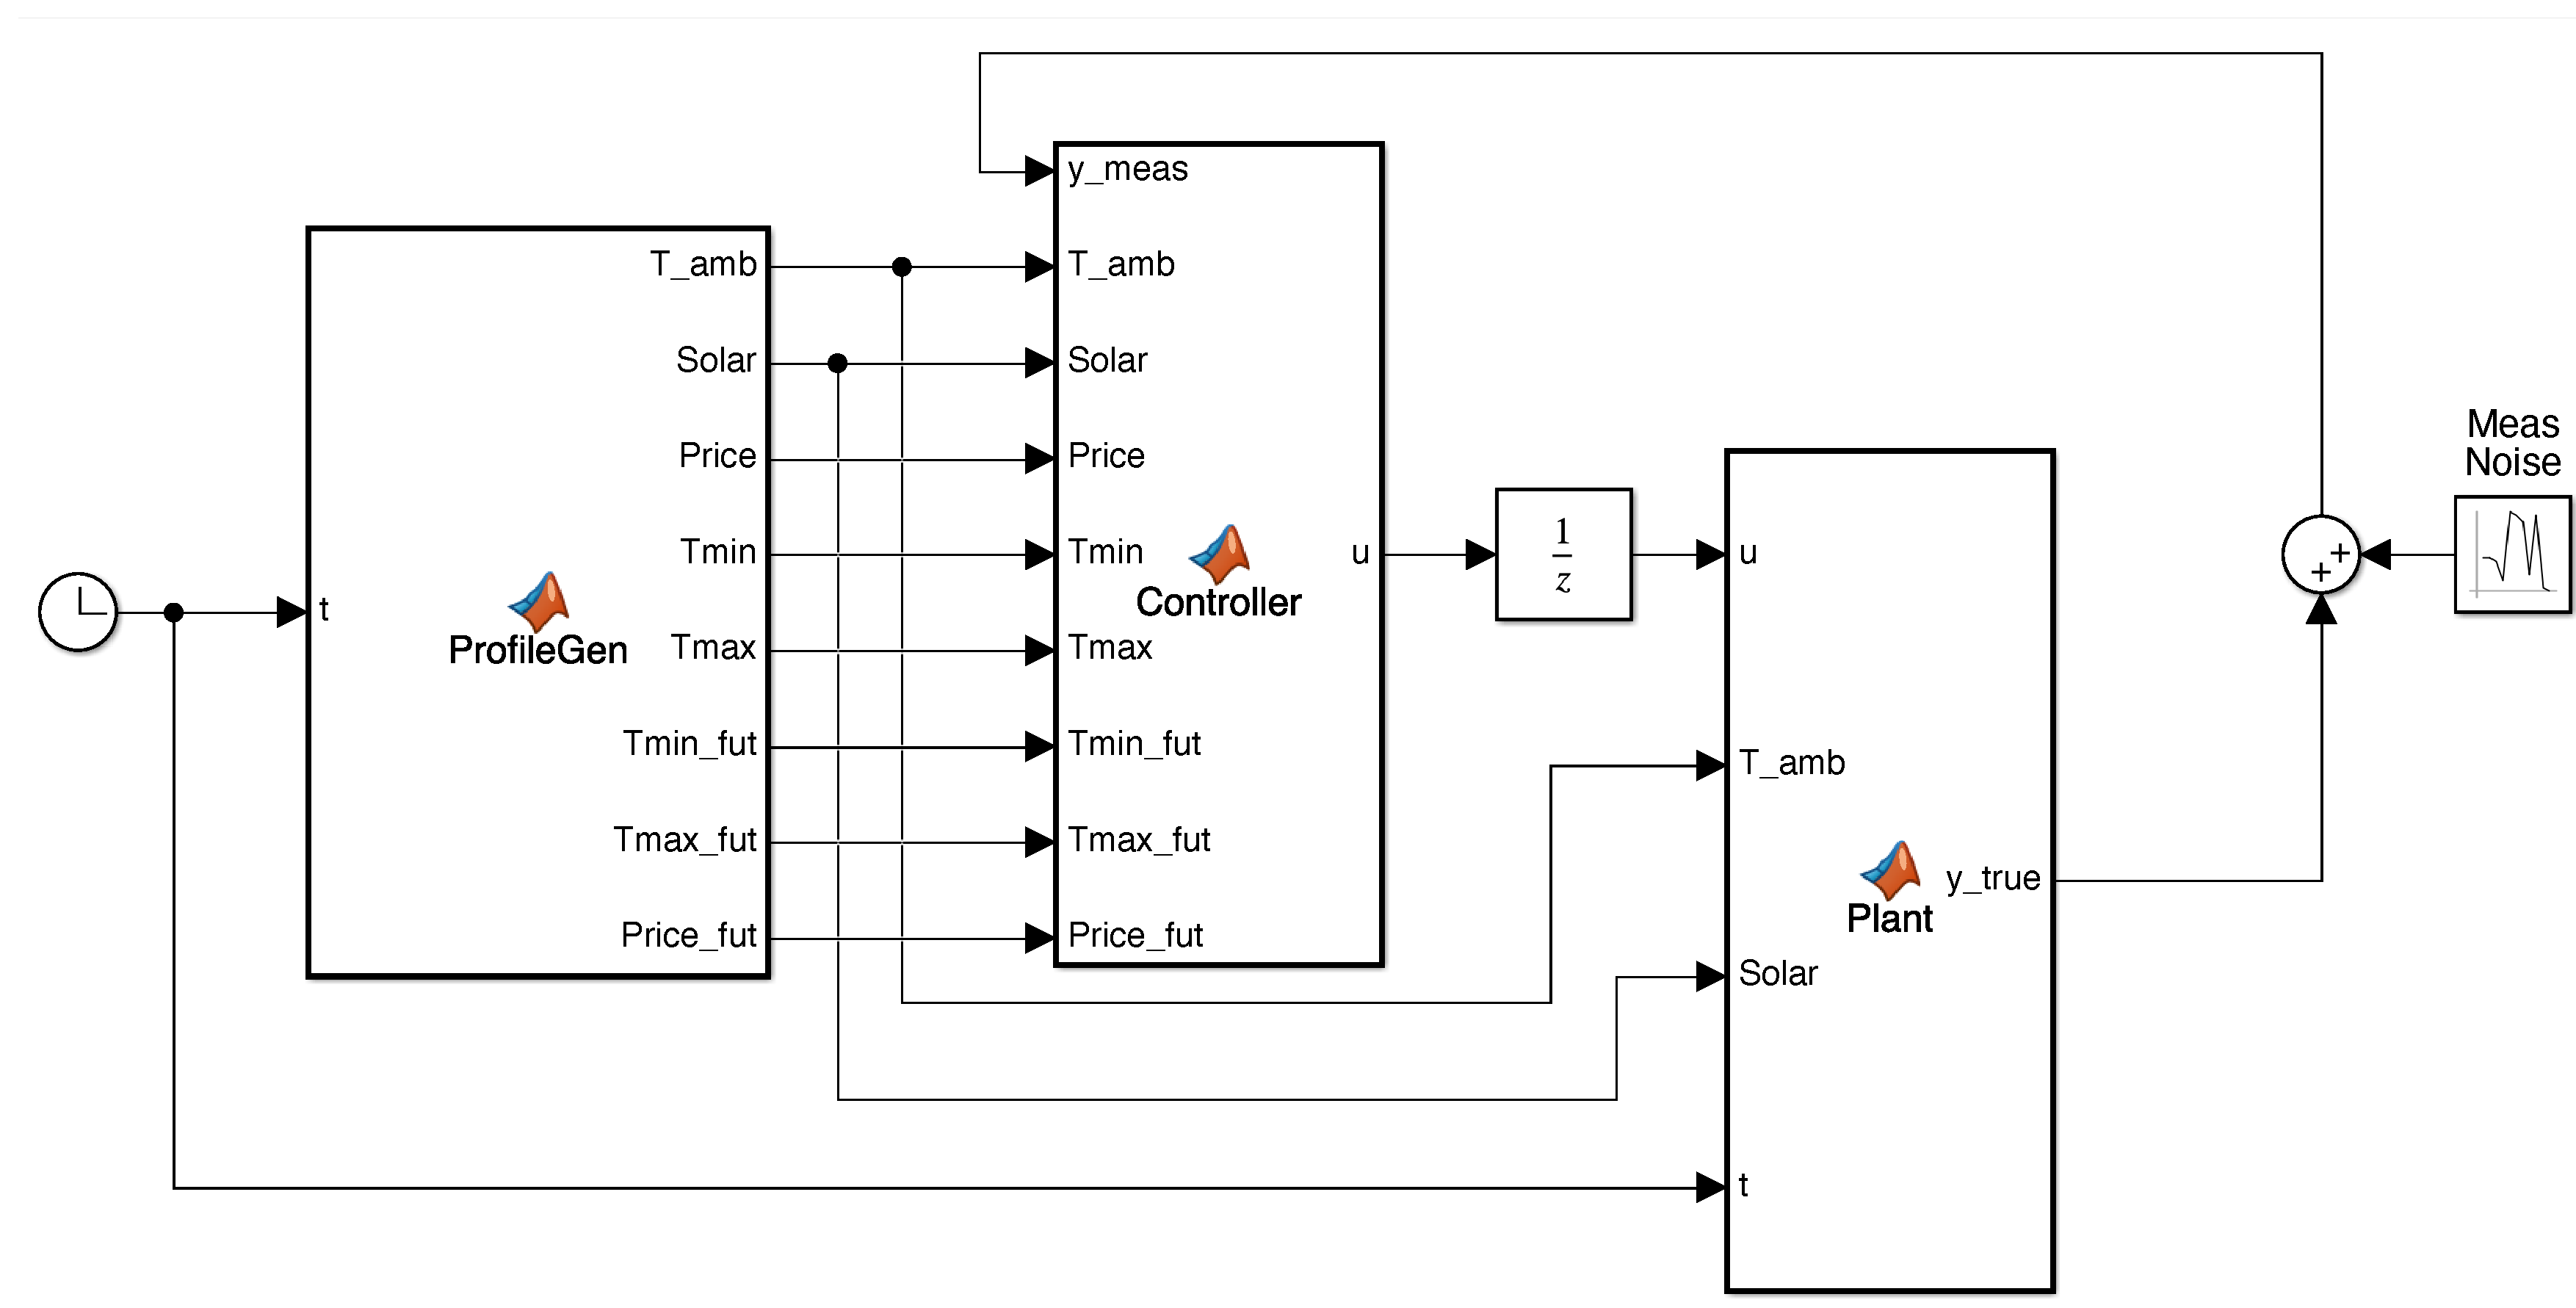
\includegraphics[width=1\linewidth]{Figures/Simulink_Building}
	\caption{HVAC Simulation using SIMULINK.}
	\label{fig:simulinkbuilding}
\end{figure}



\begin{table}[htbp]
	\centering
	\caption{Common issues and remedies for the Simulink single-zone MPC
		implementation.}
	\label{tab:troubleshoot}
	\begin{tabular}{>{\small}p{4.8cm} >{\small}p{8.8cm}}
		\toprule
		\textbf{Symptom} & \textbf{Remedy} \\
		\midrule
		\texttt{Function not found: get\_profiles} &
		Helper files are not on the MATLAB path.  Run \texttt{addpath(pwd)} or
		place all \texttt{.m} files alongside \texttt{EconomicMPC.slx}. \\[6pt]
		\texttt{Undefined function 'sdpvar'} &
		YALMIP is not installed or not on the path.  Run \texttt{yalmiptest}
		before starting Simulink. \\[6pt]
		Temperature starts from wrong value on second run &
		Persistent variables were not cleared.  Run
		\texttt{clear plant\_step mpc\_controller\_step} before pressing
		\textit{Run}. \\[6pt]
		Algebraic loop warning &
		Unit Delay block ($T_s=1800$, IC\,$=0$) is missing on the Saturation
		$\to$ Plant path.  See Section~\ref{subsec:algloop_general}. \\[6pt]
		Port dimension mismatch on \texttt{Tmin\_fut} or \texttt{Price\_fut} &
		Pre-allocation lines \texttt{Tmin\_fut = zeros(1,24)} and
		\texttt{Price\_fut = zeros(1,24)} must appear \emph{before} the
		extrinsic call in the ProfileGen wrapper. \\[6pt]
		Controller uses wrong disturbance level at night &
		Confirm the augmented model includes the correct $B_w$ column and
		that \texttt{d\_hat} (not \texttt{d\_filt}) is passed to the target
		calculator; the single-zone example does not apply exponential
		smoothing. \\[6pt]
		First step takes over 60\,s &
		Normal on low-end hardware; YALMIP is building QP matrices
		symbolically.  Do not interrupt the simulation. \\
		\bottomrule
	\end{tabular}
\end{table}


\subsection{Summary}
\label{subsec:summary}
% 

\begin{summarybox}{Simulink MPC Without the MPC Toolbox — Key Steps}
	\begin{enumerate}[noitemsep]
		\item \textbf{Helper files.}  Place all YALMIP and solver logic in
		ordinary \texttt{.m} files on the MATLAB path (Layer 2).
		\item \textbf{Persistent state.}  Store the observer state, last
		applied input, filtered disturbance, and compiled
		\texttt{optimizer} objects as \texttt{persistent} variables.
		\item \textbf{One-time compilation.}  Call
		\texttt{build\_mpc\_optimizers} on the first step only,
		guarded by \texttt{if isempty(...)}.
		\item \textbf{Wrapper blocks.}  Each Simulink MATLAB Function block
		(Layer 1) declares its helper as \texttt{coder.extrinsic},
		pre-allocates outputs, and calls the helper.
		\item \textbf{Break the algebraic loop.}  Insert a Unit Delay
		($T_s = 1800$, IC\,$= 0$) between Saturation and Plant.
		\item \textbf{Reset before each run.}  Execute
		\texttt{clear plant\_step mpc\_controller\_step} before
		pressing \textit{Run}.
	\end{enumerate}
\end{summarybox}

\section*{Chapter Summary}
\begin{itemize}
    \item Simulink integration allows MPC algorithms written in MATLAB to run inside block-diagram simulations alongside continuous-time plant models.
    \item MATLAB Function blocks embed custom MATLAB code in Simulink and interface with the solver through input and output ports.
    \item The \texttt{coder.extrinsic} directive marks functions (e.g.\ YALMIP calls) that cannot be compiled, forcing Simulink to evaluate them in the MATLAB interpreter at each time step.
    \item Persistent variables declared inside a MATLAB Function block retain their values across simulation steps, enabling stateful operations such as observer updates.
    \item The YALMIP \texttt{optimizer} object pre-compiles the QP structure once and accepts parameter updates at each call, significantly reducing per-step overhead in Simulink.
    \item A building energy MPC case study demonstrates zone temperature regulation under occupancy-driven comfort constraints and time-varying electricity pricing.
    \item The recommended simulation workflow includes model setup, controller block configuration, closed-loop wiring, and post-simulation plotting for verification.
\end{itemize}

% ─────────────────────────────────────────────────────────────
\section*{Exercises}
\label{sec:simulink_mpc_exercises}
% ─────────────────────────────────────────────────────────────

\begin{enumerate}

	\item \textbf{Persistent variables in Simulink MATLAB Function blocks.}
	In the single-zone building example, the function
	\texttt{mpc\_controller\_step} declares several \texttt{persistent}
	variables (e.g.\ the observer state~$\hat x$, the last applied
	input~$u_{k-1}$, and the compiled \texttt{optimizer} object).
	\begin{enumerate}
		\item Explain why ordinary local variables would fail to preserve
		      state across successive Simulink time steps.
		\item What would happen if the compiled \texttt{optimizer} object
		      were \emph{not} stored as a persistent variable?  Discuss the
		      implications for both correctness and computational cost.
		\item Describe the role of the \texttt{if isempty(...)} guard that
		      protects the one-time initialisation of persistent variables.
		      Why is this pattern preferred over, for example, using a
		      separate Simulink \textit{InitFcn} callback?
	\end{enumerate}

	\item \textbf{The role of \texttt{coder.extrinsic}.}
	Simulink MATLAB Function blocks are processed by MATLAB Coder, which
	requires statically typed, code-generation--compatible functions.
	\begin{enumerate}
		\item Explain why YALMIP functions (such as \texttt{sdpvar},
		      \texttt{optimize}, and \texttt{optimizer}) cannot be compiled
		      by MATLAB Coder.
		\item Describe what the \texttt{coder.extrinsic} directive does and
		      how it allows YALMIP-based helper functions to be called from
		      within a Simulink MATLAB Function block.
		\item The chapter recommends pre-allocating every output variable
		      with \texttt{zeros} \emph{before} the call to the extrinsic
		      helper.  Explain why this pre-allocation step is necessary and
		      what error would occur without it.
	\end{enumerate}

	\item \textbf{Adding a rate-of-change constraint to the building
	controller.}
	The MPC formulation in Section~\ref{sec:simulink_building} enforces box
	constraints $0 \le u_k \le 2000$\,W on the heater input but does not
	limit how quickly the input may change between consecutive steps.
	Suppose you wish to add the constraint
	$|\Delta u_k| = |u_k - u_{k-1}| \le \Delta u_{\max}$
	with $\Delta u_{\max} = 500$\,W.
	\begin{enumerate}
		\item Describe which file(s) in the two-layer architecture you would
		      need to modify and what YALMIP constraints you would add inside
		      the prediction-horizon loop.
		\item Explain why the persistent variable \texttt{u\_prev} (the last
		      applied input) must be passed as a \emph{parameter} to the
		      \texttt{optimizer} object so that the rate constraint can
		      reference the transition from $u_{k-1}$ to the first predicted
		      input $u_0$.
		\item Discuss qualitatively how adding a tight rate-of-change limit
		      would affect the closed-loop temperature response during
		      morning warm-up, when a large step in heating power would
		      otherwise be applied.
	\end{enumerate}

	\item \textbf{The algebraic-loop problem and the Unit Delay solution.}
	Section~\ref{sec:simulink_general} explains that a direct connection
	from the MPC controller output to the plant input, and from the plant
	output back to the controller, creates an algebraic loop.
	\begin{enumerate}
		\item Draw a simplified signal-flow diagram showing the loop and
		      explain, in your own words, why Simulink cannot determine a
		      consistent set of signals at a single time step when the loop
		      is present.
		\item Explain how inserting a Unit Delay block (with sample time
		      $T_s = 1800$\,s and initial condition $u_0 = 0$) breaks the
		      algebraic loop.  What is the physical interpretation of
		      applying the control action one sample period later?
		\item In practice, MPC already computes the control move for the
		      \emph{current} time step.  Argue whether the one-step delay
		      introduced by the Unit Delay block materially degrades
		      closed-loop performance for a slowly varying building thermal
		      system with a 30-minute sample time.
	\end{enumerate}

	\item \textbf{Designing a Simulink MPC architecture for a DC motor.}
	Consider a DC motor whose angular velocity $\omega$ is governed by the
	simplified continuous-time transfer function
	\[
		G(s) = \frac{\omega(s)}{V(s)} = \frac{K}{\tau s + 1},
	\]
	where $V$ is the armature voltage, $K = 10$\,rad\,s$^{-1}$\,V$^{-1}$,
	and $\tau = 0.1$\,s.  The input is subject to
	$0 \le V \le 24$\,V, and the objective is to track a reference speed
	$\omega_{\mathrm{ref}}(t)$.
	\begin{enumerate}
		\item Discretise the plant with a suitable sample time (justify your
		      choice) and write down the resulting state-space matrices
		      $A_d$, $B_d$, $C_d$, $D_d$.
		\item Sketch a Simulink block diagram following the two-layer
		      architecture from this chapter.  Label each block
		      (\textit{Reference Generator}, \textit{MPC Controller},
		      \textit{DC Motor Plant}, \textit{Scope / To Workspace}) and
		      indicate where a Unit Delay block should be placed.
		\item List the persistent variables you would declare inside the
		      \texttt{mpc\_controller\_step} function for this system.
		      Identify any differences from the building-heating case study
		      (e.g.\ is a disturbance observer still needed?).
		\item Briefly discuss how the much shorter time constant of the DC
		      motor ($\tau = 0.1$\,s) compared with the building
		      ($\tau \approx 10^4$\,s) affects the choice of prediction
		      horizon and the computational burden of solving the QP at each
		      step.
	\end{enumerate}

\end{enumerate}
	\chapter{Robust MPC and Tube MPC\texorpdfstring{$^{(*)}$}{(*)}}
\label{chap:tube_mpc}

\begin{quote}
	\textit{``Standard MPC tells you the best thing to do if the world is perfect. Tube MPC tells you what to do when it isn't.''} \\
	\hfill --- paraphrasing \textbf{David Q.\ Mayne}
\end{quote}

Every MPC formulation we have seen so far relies on a perfect model: $x_{k+1} = Ax_k + Bu_k$. The controller solves an optimisation, applies the first input, and re-solves at the next step. This works well in practice --- \emph{provided the model is accurate}. In practice, however, systems are always subject to disturbances: sensor noise, wind gusts, friction that the model ignores, or small inaccuracies in the $A$ and $B$ matrices themselves. Even a tiny modelling error, accumulated over many steps, can push the real state across a constraint boundary that the controller thought was safe.

This chapter addresses the question: \textbf{how do we guarantee constraint satisfaction when the model is not perfect?} The answer is \emph{robust MPC}, and the most practical and widely-used form is called \textbf{Tube MPC}, introduced by Langson et al.~\cite{Langson2004} and further developed by Mayne et al.~\cite{Mayne2005}. The central idea is straightforward: instead of planning a single trajectory, we plan a ``tube'' of trajectories. As long as the disturbance is bounded, the real trajectory stays inside the tube, and the tube is designed so that constraints are never violated.

\section{The Problem: Disturbances and Constraint Violations}
\label{sec:tube_problem}

Consider the linear system with an additive disturbance:
\begin{equation} \label{eq:uncertain_system}
	x_{k+1} = Ax_k + Bu_k + w_k
\end{equation}
where $x_k \in \mathbb{R}^n$ is the state, $u_k \in \mathbb{R}^m$ is the control input, and $w_k \in \mathbb{R}^n$ is a disturbance. We assume:
\begin{itemize}[noitemsep]
	\item The disturbance is bounded: $w_k \in \mathcal{W}$ for all $k \ge 0$, where $\mathcal{W}$ is a known convex polytope containing the origin (e.g., $\|w_k\|_\infty \le \delta$ for some known $\delta > 0$).
	\item We do \emph{not} know the specific value of $w_k$ in advance. We only know it will lie somewhere in $\mathcal{W}$.
\end{itemize}

The system is subject to constraints:
\[
x_k \in \mathcal{X}, \qquad u_k \in \mathcal{U}, \qquad \text{for all } k \ge 0
\]

\subsection*{Why Standard MPC Fails}

Standard MPC ignores $w_k$ and plans as if $x_{k+1} = Ax_k + Bu_k$. At each step, it re-measures the state and re-solves, which provides some natural robustness. However, this is not enough to \emph{guarantee} constraint satisfaction.

Suppose the MPC plans a trajectory that passes close to a constraint boundary --- say $x_1 \le 5$. The controller predicts $x_1 = 4.95$ and decides this is safe. But after the input is applied, the disturbance $w_0$ adds an unexpected $+0.1$ to the state, producing $x_1 = 5.05$. The constraint is violated.

Standard MPC cannot prevent this because it does not account for the ``worst case'' during planning. It optimistically assumes the prediction is exact.

\begin{alertbox}{The core difficulty}
	Standard MPC guarantees constraints are satisfied for the \emph{predicted} trajectory. But when disturbances act, the \emph{actual} trajectory deviates from the prediction. No amount of re-solving at the next step can undo a constraint violation that has already occurred.
\end{alertbox}

\section{Two Approaches to Robust MPC}

Two main approaches exist for handling bounded disturbances.

\subsection{Min--Max MPC}

The most direct approach formulates the problem as a game between the controller and an adversary (nature). The controller chooses inputs $u$ to minimise the cost, while nature chooses disturbances $w \in \mathcal{W}$ to maximise it:
\[
\min_{u_0, \ldots, u_{N-1}} \;\max_{w_0, \ldots, w_{N-1} \in \mathcal{W}} \; J(x, u)
\]
subject to the dynamics~\eqref{eq:uncertain_system} and the constraints $x_k \in \mathcal{X}$, $u_k \in \mathcal{U}$ for all possible disturbance realisations.

This is mathematically rigorous but has serious drawbacks:
\begin{itemize}[noitemsep]
	\item \textbf{Computational explosion.} The disturbance branches at every time step. Over $N$ steps with $d$ possible disturbance vertices, the number of scenarios grows as $d^N$. For even modest problems, this becomes intractable.
	\item \textbf{Conservatism.} The controller assumes nature is adversarial and always picks the worst disturbance. In reality, disturbances are often random, not adversarial. The resulting controller is overly cautious.
\end{itemize}

Min--max MPC is therefore rarely used in practice. It is included here for completeness and to motivate the more practical alternative.

\subsection{Tube MPC: The Key Idea}

Tube MPC avoids the computational explosion by separating the problem into two parts:
\begin{enumerate}
	\item A \textbf{nominal trajectory} $z_k$ that is planned as if there were no disturbance. This is a standard MPC problem.
	\item A \textbf{feedback controller} $-K(x_k - z_k)$ that keeps the real state $x_k$ close to the nominal trajectory $z_k$, despite the disturbance.
\end{enumerate}

\begin{notebox}{Notation: $z_k$ in This Chapter}
	Throughout this chapter, $z_k$ denotes the \textbf{nominal state} (the disturbance-free planned trajectory). This is unrelated to the augmented state vector $z_k = [x_k^\top\;\; d_k^\top]^\top$ used in the offset-free MPC formulation of Chapter~\ref{chap:output_fb_mpc}. The two uses of $z_k$ never appear in the same context.
\end{notebox}

The deviation $e_k = x_k - z_k$ between the real and nominal state is bounded because $K$ is stabilising and the disturbance is bounded. The set of all possible deviations forms a ``tube'' around the nominal trajectory. By tightening the constraints on the nominal trajectory (shrinking them inward by the tube width), we guarantee that the real trajectory satisfies the original constraints.

This is the essence of Tube MPC: \textbf{plan the nominal path conservatively, and let a feedback controller handle the disturbances.}

\section{Set Operations: Minkowski Sum and Pontryagin Difference}

Before developing Tube MPC formally, we need two set operations that appear throughout the theory. These are not difficult, but they are essential.

\subsection{Minkowski Sum}

\begin{defnbox}{Definition: Minkowski Sum}
	The \textbf{Minkowski sum} of two sets $P$ and $Q$ in $\mathbb{R}^n$ is:
	\[
	P \oplus Q = \{p + q \mid p \in P, \; q \in Q\}
	\]
	In words: take every point in $P$, add every point in $Q$, and collect all the results. The resulting set is ``$P$ inflated by $Q$''.
\end{defnbox}

\textbf{Geometric intuition.} Place a copy of $Q$ at every point of $P$. The Minkowski sum is the union of all these copies. If $P$ is a square and $Q$ is a small disk, then $P \oplus Q$ is the square with rounded corners. Figure~\ref{fig:minkowski_sum} illustrates this operation.

\begin{figure}[H]
	\centering
	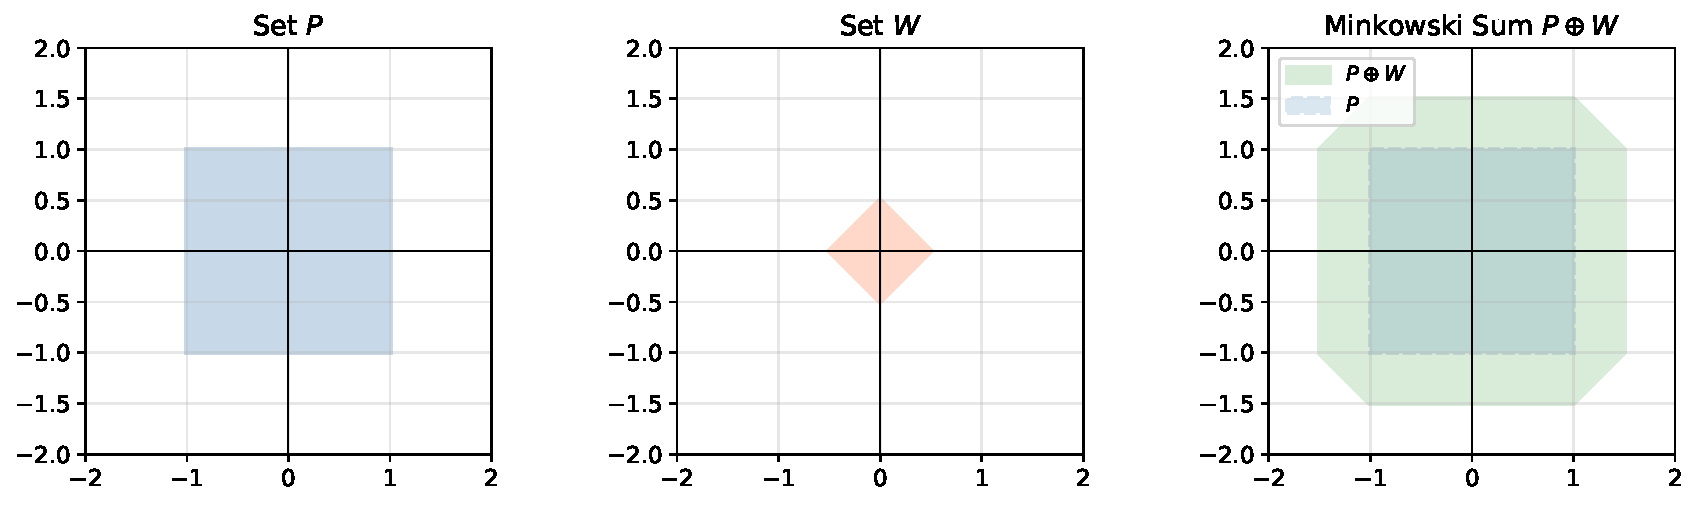
\includegraphics[width=0.95\linewidth]{Figures/minkowski_sum.pdf}
	\caption{Minkowski sum of a square $P$ and a diamond $W$. The result $P \oplus W$ is larger than $P$, ``inflated'' by the shape of $W$.}
	\label{fig:minkowski_sum}
\end{figure}

\textbf{Why it matters for Tube MPC.} If the nominal state is $z_k$ and the error $e_k$ can be anywhere in a set $\mathcal{E}$, then the actual state $x_k = z_k + e_k$ can be anywhere in $\{z_k\} \oplus \mathcal{E}$. The tube around the nominal trajectory is exactly this: the Minkowski sum of each nominal point with the error set.

\subsection{Pontryagin Difference}

\begin{defnbox}{Definition: Pontryagin Difference}
	The \textbf{Pontryagin difference} (also called the \emph{erosion}) of a set $\mathcal{X}$ by a set $\mathcal{E}$ is:
	\[
	\mathcal{X} \ominus \mathcal{E} = \{z \in \mathbb{R}^n \mid z + e \in \mathcal{X} \;\; \text{for all } e \in \mathcal{E}\}
	\]
	In words: $\mathcal{X} \ominus \mathcal{E}$ contains all points $z$ such that \emph{every possible shift by an element of $\mathcal{E}$} still lands inside $\mathcal{X}$.
\end{defnbox}

\textbf{Geometric intuition.} The Pontryagin difference is the ``shrunk'' version of $\mathcal{X}$. If you stand at a point $z \in \mathcal{X} \ominus \mathcal{E}$ and someone pushes you by any amount in $\mathcal{E}$, you still remain inside $\mathcal{X}$. It is the opposite of the Minkowski sum: while $\oplus$ inflates a set, $\ominus$ shrinks it. See Figure~\ref{fig:pontryagin_diff} for an illustration.

\begin{figure}[H]
	\centering
	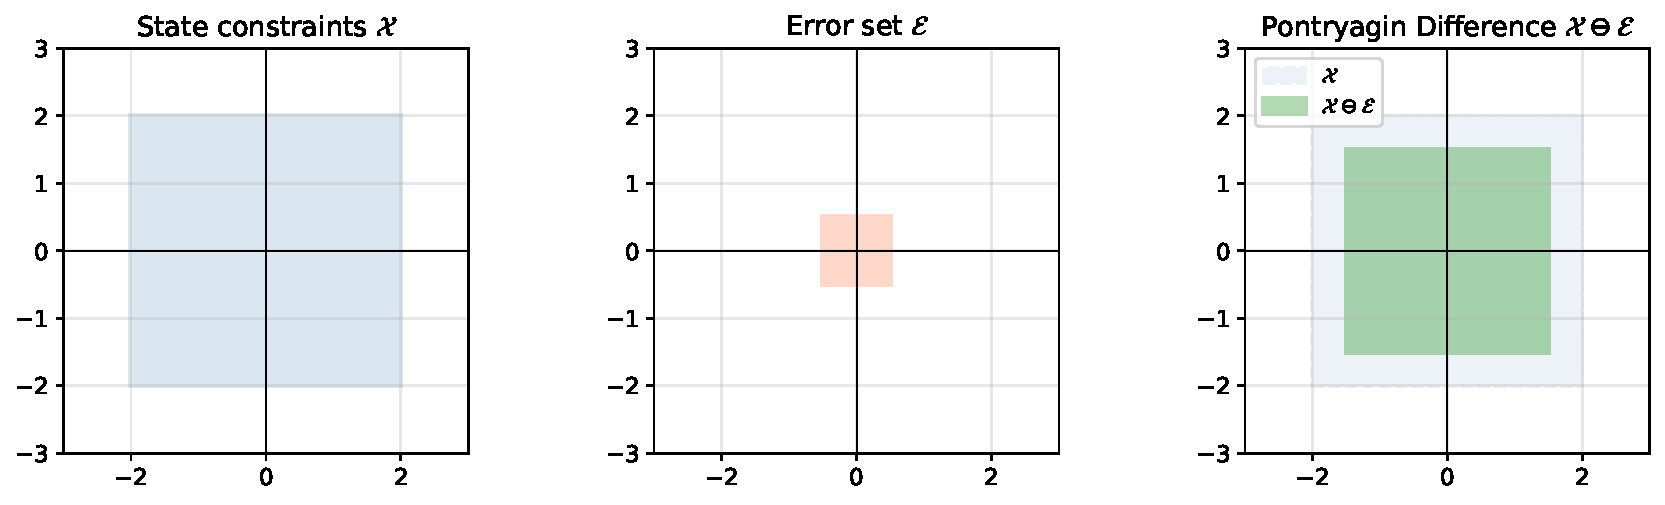
\includegraphics[width=0.95\linewidth]{Figures/pontryagin_diff.pdf}
	\caption{Pontryagin difference $\mathcal{X} \ominus \mathcal{E}$. The original constraint set $\mathcal{X}$ (dashed blue) is shrunk inward by the size of $\mathcal{E}$ (red), yielding the tightened set (solid green). Any point in the tightened set remains inside $\mathcal{X}$ even after a worst-case shift from $\mathcal{E}$.}
	\label{fig:pontryagin_diff}
\end{figure}

\textbf{Why it matters for Tube MPC.} To guarantee that the real state $x_k = z_k + e_k$ satisfies $x_k \in \mathcal{X}$ for all $e_k \in \mathcal{E}$, we must require the nominal state to satisfy $z_k \in \mathcal{X} \ominus \mathcal{E}$. This is called \emph{constraint tightening}.

\begin{examplebox}{Minkowski Sum and Pontryagin Difference in 1D}
	Let $\mathcal{X} = [-5, \; 5]$ (the state must stay between $-5$ and $5$) and $\mathcal{E} = [-0.3, \; 0.3]$ (the error is at most $0.3$ in magnitude).

	\solution

	\textbf{Minkowski sum:} $\mathcal{X} \oplus \mathcal{E} = [-5.3, \; 5.3]$. The set grows by the error width on each side.

	\textbf{Pontryagin difference:} $\mathcal{X} \ominus \mathcal{E} = [-4.7, \; 4.7]$. The set shrinks by $0.3$ on each side. If the nominal state $z$ stays within $[-4.7, 4.7]$, then $x = z + e$ stays within $[-5, 5]$ for any $|e| \le 0.3$.

	This is constraint tightening: the nominal trajectory must respect the stricter bounds $\pm 4.7$, so that the actual trajectory respects the original bounds $\pm 5$.
\end{examplebox}


\section{Tube MPC: The Full Development}
\label{sec:tube_full}

We now develop Tube MPC step by step.

\subsection{Step 1: Decompose the System}

The uncertain system is $x_{k+1} = Ax_k + Bu_k + w_k$. We introduce a \emph{nominal} system that evolves without disturbance:
\begin{equation} \label{eq:nominal_system}
	z_{k+1} = Az_k + Bv_k
\end{equation}
where $z_k$ is the nominal state and $v_k$ is the nominal input. These are the decision variables that the MPC optimiser will compute.

We define the \emph{error} between the real and nominal states:
\[
e_k = x_k - z_k
\]

The control input is split into two parts:
\begin{equation} \label{eq:tube_control_law}
	u_k = v_k - K(x_k - z_k) = v_k - Ke_k
\end{equation}
where:
\begin{itemize}[noitemsep]
	\item $v_k$ is the \textbf{nominal input}, computed by the MPC optimiser. It steers the nominal trajectory $z_k$ toward the origin.
	\item $K$ is a \textbf{fixed feedback gain} (typically the LQR gain from \texttt{dlqr}, so $K > 0$ and $u = -Kx$ stabilises the system). It keeps the real state close to the nominal state by rejecting disturbances.
\end{itemize}

\subsection{Step 2: Derive the Error Dynamics}

Substituting~\eqref{eq:tube_control_law} into the real dynamics~\eqref{eq:uncertain_system} and subtracting the nominal dynamics~\eqref{eq:nominal_system}:

\begin{align*}
	x_{k+1} &= Ax_k + B(v_k - Ke_k) + w_k \\
	z_{k+1} &= Az_k + Bv_k
\end{align*}

Subtracting:
\begin{equation} \label{eq:error_dynamics}
	\boxed{e_{k+1} = (A - BK)\,e_k + w_k}
\end{equation}

This is the key result. The error dynamics are \emph{autonomous}: they do not depend on $v_k$ at all. The nominal input cancels out. The error evolves purely under the closed-loop matrix $A_{cl} = A - BK$ and the disturbance $w_k$.

Since $K$ is chosen so that $A_{cl}$ is Schur stable (all eigenvalues inside the unit circle), the error $e_k$ does not grow without bound. But it does not converge to zero either, because the disturbance $w_k$ keeps pushing it around. Instead, $e_k$ settles into a bounded set that we can compute.

\subsection{Step 3: The Minimal Robust Positively Invariant Set}

\begin{defnbox}{Definition: Robust Positively Invariant (RPI) Set}
	A set $\mathcal{E} \subseteq \mathbb{R}^n$ is a \textbf{robust positively invariant (RPI) set} for the error dynamics $e_{k+1} = A_{cl}\,e_k + w_k$ with $w_k \in \mathcal{W}$ if:
	\[
	e_k \in \mathcal{E} \;\;\Longrightarrow\;\; e_{k+1} \in \mathcal{E} \quad \text{for all } w_k \in \mathcal{W}
	\]
	Once the error enters $\mathcal{E}$, it stays in $\mathcal{E}$ forever, no matter what disturbances occur.
\end{defnbox}

The smallest such set is the \textbf{minimal RPI (mRPI) set}, denoted $\mathcal{E}_\infty$~\cite{Rakovic2005}. It can be characterised explicitly:
\begin{equation} \label{eq:mrpi}
	\mathcal{E}_\infty = \bigoplus_{i=0}^{\infty} A_{cl}^i\, \mathcal{W} \;=\; \mathcal{W} \oplus A_{cl}\mathcal{W} \oplus A_{cl}^2\mathcal{W} \oplus \cdots
\end{equation}
where $\bigoplus$ denotes the Minkowski sum. In words: take the disturbance set $\mathcal{W}$, apply the closed-loop dynamics to get $A_{cl}\mathcal{W}$, then $A_{cl}^2\mathcal{W}$, and so on. Each set is smaller than the previous one (because $A_{cl}$ is stable and shrinks vectors). The mRPI is the Minkowski sum of all these sets.

\textbf{Why is this a valid invariant set?} If $e_k \in \mathcal{E}_\infty$, then $e_{k+1} = A_{cl}\,e_k + w_k$. Since $A_{cl}$ maps $\mathcal{E}_\infty$ into $\bigoplus_{i=1}^{\infty} A_{cl}^i\,\mathcal{W}$, and adding $w_k \in \mathcal{W}$ gives $\mathcal{W} \oplus \bigoplus_{i=1}^{\infty} A_{cl}^i\,\mathcal{W} = \mathcal{E}_\infty$, the set is invariant.

\textbf{Practical computation.} The infinite sum~\eqref{eq:mrpi} is computed by iterating:
\begin{align*}
	\Omega_0 &= \mathcal{W} \\
	\Omega_{i+1} &= \Omega_i \oplus A_{cl}^{i+1}\mathcal{W}
\end{align*}
and stopping when $\Omega_{i+1} \approx \Omega_i$ (the additional term $A_{cl}^{i+1}\mathcal{W}$ becomes negligibly small because $A_{cl}$ is stable). Figure~\ref{fig:mrpi_iteration} illustrates this convergence.

\begin{figure}[H]
	\centering
	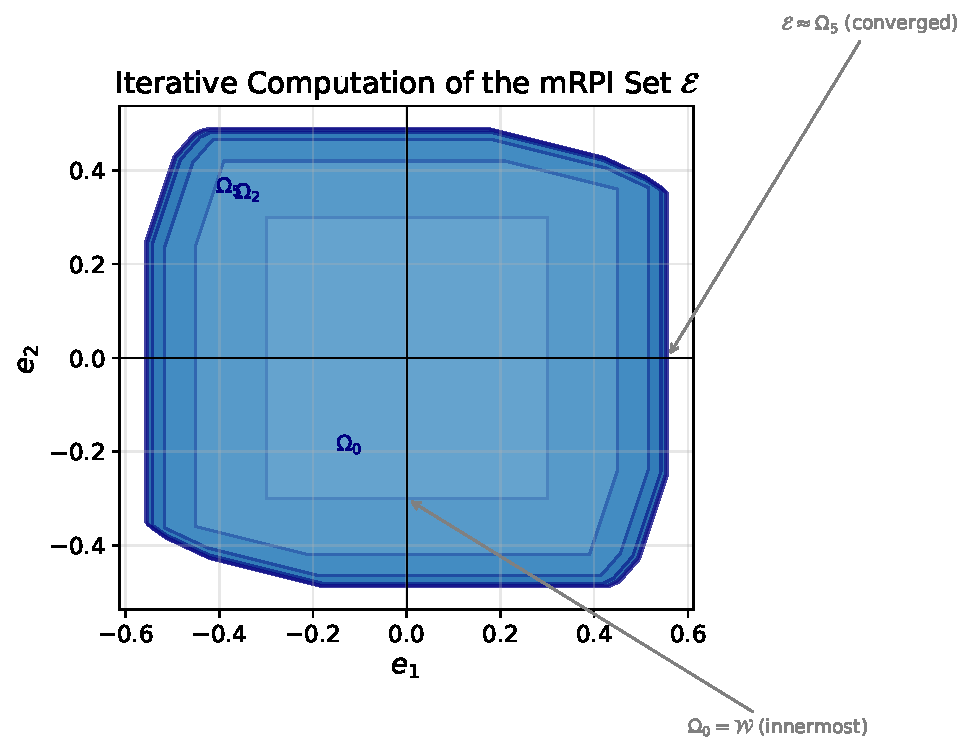
\includegraphics[width=0.6\linewidth]{Figures/mrpi_iteration.pdf}
	\caption{Iterative computation of the mRPI set. Starting from $\Omega_0 = \mathcal{W}$ (innermost set), each iteration adds a smaller and smaller set $A_{cl}^i\mathcal{W}$. The sets converge to the mRPI set $\mathcal{E}_\infty$.}
	\label{fig:mrpi_iteration}
\end{figure}

\textbf{The role of $K$.} A faster stabilising gain $K$ (one that places the eigenvalues of $A_{cl}$ closer to zero) produces a smaller mRPI set $\mathcal{E}_\infty$, because $A_{cl}^i\mathcal{W}$ shrinks faster. A smaller tube means less constraint tightening, which means a larger feasible region for the nominal MPC. However, aggressive gains require larger control inputs, which tightens the input constraints more. There is a trade-off in choosing $K$.

\begin{examplebox}{Computing the mRPI Set for a Scalar System}
	Consider the scalar system $x_{k+1} = 1.2\,x_k + u_k + w_k$ with $|w_k| \le 0.1$ and $|u_k| \le 1$. The stabilising gain is $K = 0.79$ (as returned by \texttt{dlqr}, so $u = -Kx$), giving $a_{cl} = 1.2 - 0.79 = 0.41$.

	\solution

	The mRPI set is the interval $\mathcal{E}_\infty = [-\bar{e}, \;\bar{e}]$, where:
	\[
	\bar{e} = \sum_{i=0}^{\infty} |a_{cl}|^i \cdot 0.1 = \frac{0.1}{1 - |a_{cl}|} = \frac{0.1}{1 - 0.41} = \frac{0.1}{0.59} \approx 0.169
	\]

	So the error $e_k = x_k - z_k$ is guaranteed to stay within $[-0.169, \; 0.169]$, no matter what disturbance sequence occurs (as long as $|w_k| \le 0.1$).

	\textbf{Constraint tightening.} If the original input constraint is $|u_k| \le 1$, the tightened input constraint for $v_k$ is:
	\[
	|v_k| \le 1 - |K| \cdot \bar{e} = 1 - 0.79 \times 0.169 \approx 0.867
	\]

	If the state constraint is $|x_k| \le 5$, the tightened state constraint for $z_k$ is:
	\[
	|z_k| \le 5 - 0.169 = 4.831
	\]

	The nominal MPC plans with these tighter bounds, and the feedback controller $u_k = v_k - K(x_k - z_k)$ takes care of the rest.
\end{examplebox}


\section{Step 4: Constraint Tightening}
\label{sec:constraint_tightening}

This is the central mechanism that makes Tube MPC robust. Since the real state $x_k = z_k + e_k$ can deviate from the nominal state $z_k$ by any amount in $\mathcal{E}$, we must ensure the constraints hold even in the worst case.

\textbf{State constraints.} We need $x_k = z_k + e_k \in \mathcal{X}$ for all $e_k \in \mathcal{E}$. This is equivalent to requiring:
\begin{equation}
	z_k \in \mathcal{X} \ominus \mathcal{E} \;=:\; \mathcal{X}_t
\end{equation}
The tightened state constraint set $\mathcal{X}_t$ is the original constraint set shrunk by the tube width.

\textbf{Input constraints.} The actual input is $u_k = v_k - Ke_k$. We need $u_k \in \mathcal{U}$ for all $e_k \in \mathcal{E}$. This gives:
\begin{equation}
	v_k \in \mathcal{U} \ominus K\mathcal{E} \;=:\; \mathcal{V}
\end{equation}
where $K\mathcal{E} = \{Ke \mid e \in \mathcal{E}\}$ is the set of all possible feedback corrections.

\textbf{Why does this work?} By construction:
\begin{itemize}[noitemsep]
	\item If $z_k \in \mathcal{X}_t$ and $e_k \in \mathcal{E}$, then $x_k = z_k + e_k \in \mathcal{X}$. \hfill (Definition of $\ominus$.)
	\item If $v_k \in \mathcal{V}$ and $e_k \in \mathcal{E}$, then $u_k = v_k - Ke_k \in \mathcal{U}$. \hfill (Definition of $\ominus$.)
\end{itemize}

The original hard constraints on $(x_k, u_k)$ are \emph{guaranteed} to be satisfied, regardless of which disturbance $w_k \in \mathcal{W}$ occurs. The price we pay is that the nominal trajectory has less room: the feasible region shrinks by the tube width on all sides.

\begin{notebox}{How much room do we lose?}
	The amount of constraint tightening depends directly on the size of $\mathcal{E}$, which in turn depends on:
	\begin{itemize}[noitemsep]
		\item \textbf{The disturbance bound $\mathcal{W}$}: Larger disturbances $\Rightarrow$ larger $\mathcal{E}$ $\Rightarrow$ more tightening.
		\item \textbf{The feedback gain $K$}: A faster gain shrinks $\mathcal{E}$ (less tightening of state constraints) but enlarges $K\mathcal{E}$ (more tightening of input constraints). A slower gain has the opposite effect.
	\end{itemize}

	In the extreme case where $\mathcal{W} = \{0\}$ (no disturbance), we get $\mathcal{E} = \{0\}$, and the tightened constraints equal the original constraints. Tube MPC reduces to standard MPC.
\end{notebox}


\section{Step 5: The Tube MPC Optimisation Problem}
\label{sec:tube_opt}

At each time step $k$, we measure the current state $x_k$ and solve the following optimisation over the nominal trajectory $(z, v)$:

\begin{equation} \label{eq:tube_mpc_opt}
	\begin{aligned}
		\min_{z_0, \ldots, z_N, \;\; v_0, \ldots, v_{N-1}} \quad & z_N^\top P\, z_N + \sum_{i=0}^{N-1} \bigl(z_i^\top Q\, z_i + v_i^\top R\, v_i\bigr) \\[6pt]
		\text{subject to:} \quad
		& z_{i+1} = Az_i + Bv_i, \qquad i = 0, \ldots, N-1 \\
		& z_i \in \mathcal{X}_t = \mathcal{X} \ominus \mathcal{E}, \qquad i = 0, \ldots, N-1 \\
		& v_i \in \mathcal{V} = \mathcal{U} \ominus K\mathcal{E}, \qquad i = 0, \ldots, N-1 \\
		& z_N \in \mathcal{X}_f \\
		& x_k \in z_0 \oplus \mathcal{E}
	\end{aligned}
\end{equation}

The key differences from standard MPC are:
\begin{enumerate}
	\item \textbf{The optimisation is over the nominal system} $(z, v)$, not the real system $(x, u)$. The nominal system has no disturbance, so this is a standard QP --- exactly the same type of problem we solved in Chapter~7.

	\item \textbf{The constraints are tightened.} The state and input constraints are shrunk inward by the tube width to account for the worst-case disturbance.

	\item \textbf{The initial condition links the nominal and real systems.} The constraint $x_k \in z_0 \oplus \mathcal{E}$ ensures the nominal starting point $z_0$ is close enough to the measured state $x_k$ that the error $e_0 = x_k - z_0$ lies within $\mathcal{E}$. In practice, this is often implemented by fixing $z_0 = x_k$ (which satisfies the constraint since $0 \in \mathcal{E}$), or by optimising over $z_0$ (which can improve performance by choosing a better tube centre).

	\item \textbf{The terminal set $\mathcal{X}_f$} is a positive invariant set for the nominal system under the tightened constraints, analogous to the terminal set in Chapter~7. It must satisfy $\mathcal{X}_f \subseteq \mathcal{X}_t$.
\end{enumerate}

After solving~\eqref{eq:tube_mpc_opt}, the control input applied to the real system is:
\begin{equation}
	u_k = v_0^\star - K(x_k - z_0^\star)
\end{equation}

At the next time step, we re-measure $x_{k+1}$ and solve again.


\section{Tube MPC Architecture}
\label{sec:tube_architecture}

The complete Tube MPC controller has the following structure:

\begin{center}
	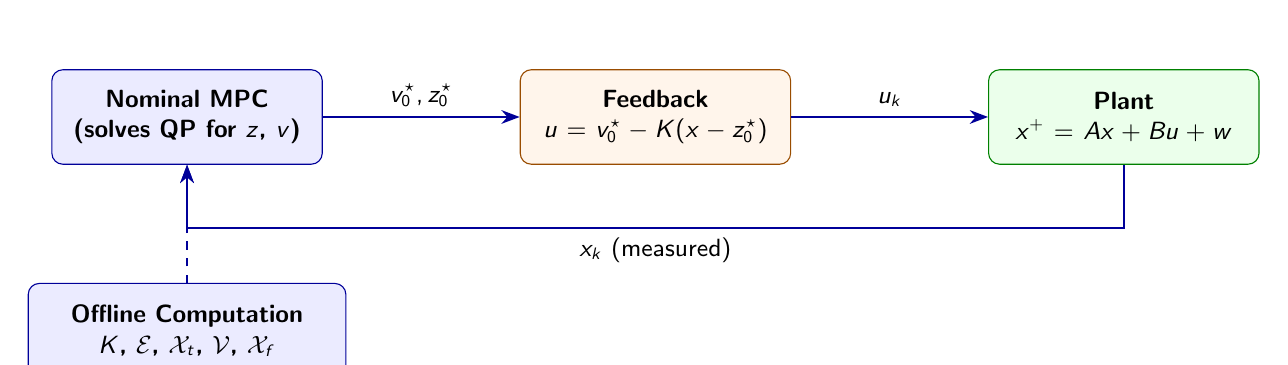
\begin{tikzpicture}[
		block/.style={rectangle, rounded corners=4pt, draw=blue!60!black, fill=blue!8,
			text width=3.2cm, minimum height=1.2cm, align=center, font=\small\bfseries\sffamily},
		greenblock/.style={block, draw=green!50!black, fill=green!8},
		orangeblock/.style={block, draw=orange!60!black, fill=orange!8},
		arrow/.style={-Stealth, thick, draw=blue!60!black},
		]

		% Blocks
		\node[block] (mpc) {Nominal MPC\\(solves QP for $z$, $v$)};
		\node[orangeblock, right=2.5cm of mpc] (feedback) {Feedback\\$u = v_0^\star - K(x - z_0^\star)$};
		\node[greenblock, right=2.5cm of feedback] (plant) {Plant\\$x^+ = Ax + Bu + w$};

		% Offline block
		\node[block, below=1.5cm of mpc, text width=3.8cm] (offline) {Offline Computation\\$K$, $\mathcal{E}$, $\mathcal{X}_t$, $\mathcal{V}$, $\mathcal{X}_f$};

		% Arrows
		\draw[arrow] (mpc) -- node[above, font=\small\sffamily] {$v_0^\star, z_0^\star$} (feedback);
		\draw[arrow] (feedback) -- node[above, font=\small\sffamily] {$u_k$} (plant);
		\draw[arrow] (plant.south) -- ++(0,-0.8) -| node[below, near start, font=\small\sffamily] {$x_k$ (measured)} (mpc.south);
		\draw[arrow, dashed] (offline) -- (mpc);
	\end{tikzpicture}
\end{center}

The offline computation (feedback gain $K$, mRPI set $\mathcal{E}$, tightened constraints $\mathcal{X}_t$ and $\mathcal{V}$, and the terminal set $\mathcal{X}_f$) is performed once during the design phase. At run time, the controller only needs to solve the nominal QP (same size as standard MPC) and add the feedback correction.


\section{Worked Example: Tube MPC for a Scalar System}
\label{sec:tube_example_scalar}

\begin{examplebox}{Tube MPC: Scalar Integrator with Disturbance}
	Consider the system:
	\[
	x_{k+1} = 1.2\,x_k + u_k + w_k
	\]
	with $|u_k| \le 1$, $|x_k| \le 5$, $|w_k| \le 0.1$, and initial condition $x_0 = 2$.

	Design a Tube MPC controller with $Q = 1$, $R = 1$, $N = 5$.

	\solution

	\textbf{Step 1: Choose $K$ and compute the closed-loop eigenvalue.}

	Using the DARE with $Q = 1$, $R = 1$: $K = 0.79$ (positive, as returned by \texttt{dlqr}), so $u = -Kx \approx -0.79x$, giving $a_{cl} = a - bK = 1.2 - 0.79 = 0.41$.

	\textbf{Step 2: Compute the mRPI set.}
	\[
	\bar{e} = \frac{w_{\max}}{1 - |a_{cl}|} = \frac{0.1}{1 - 0.41} = \frac{0.1}{0.59} \approx 0.169
	\]
	So $\mathcal{E} = [-0.169, \; 0.169]$.

	\textbf{Step 3: Tighten constraints.}
	\begin{align*}
		\text{State:} \quad & |z_k| \le 5 - 0.169 = 4.831 \\
		\text{Input:} \quad & |v_k| \le 1 - |K| \cdot \bar{e} = 1 - 0.79 \times 0.169 \approx 0.867
	\end{align*}

	\textbf{Step 4: Solve the nominal MPC.}

	At each time step, solve the standard MPC problem~\eqref{eq:tube_mpc_opt} for the disturbance-free system $z_{k+1} = 1.2\,z_k + v_k$ with the tightened constraints $|z_k| \le 4.831$ and $|v_k| \le 0.867$.

	\textbf{Step 5: Apply the tube control law.}
	\[
	u_k = v_k^\star - K(x_k - z_k^\star) = v_k^\star - 0.79(x_k - z_k^\star)
	\]

	Figure~\ref{fig:tube_scalar} shows 50 different disturbance realisations. The blue traces are the actual state trajectories; the red dashed line is the nominal trajectory. All realisations remain within the constraint bounds, despite the disturbances.
\end{examplebox}

\begin{figure}[H]
	\centering
	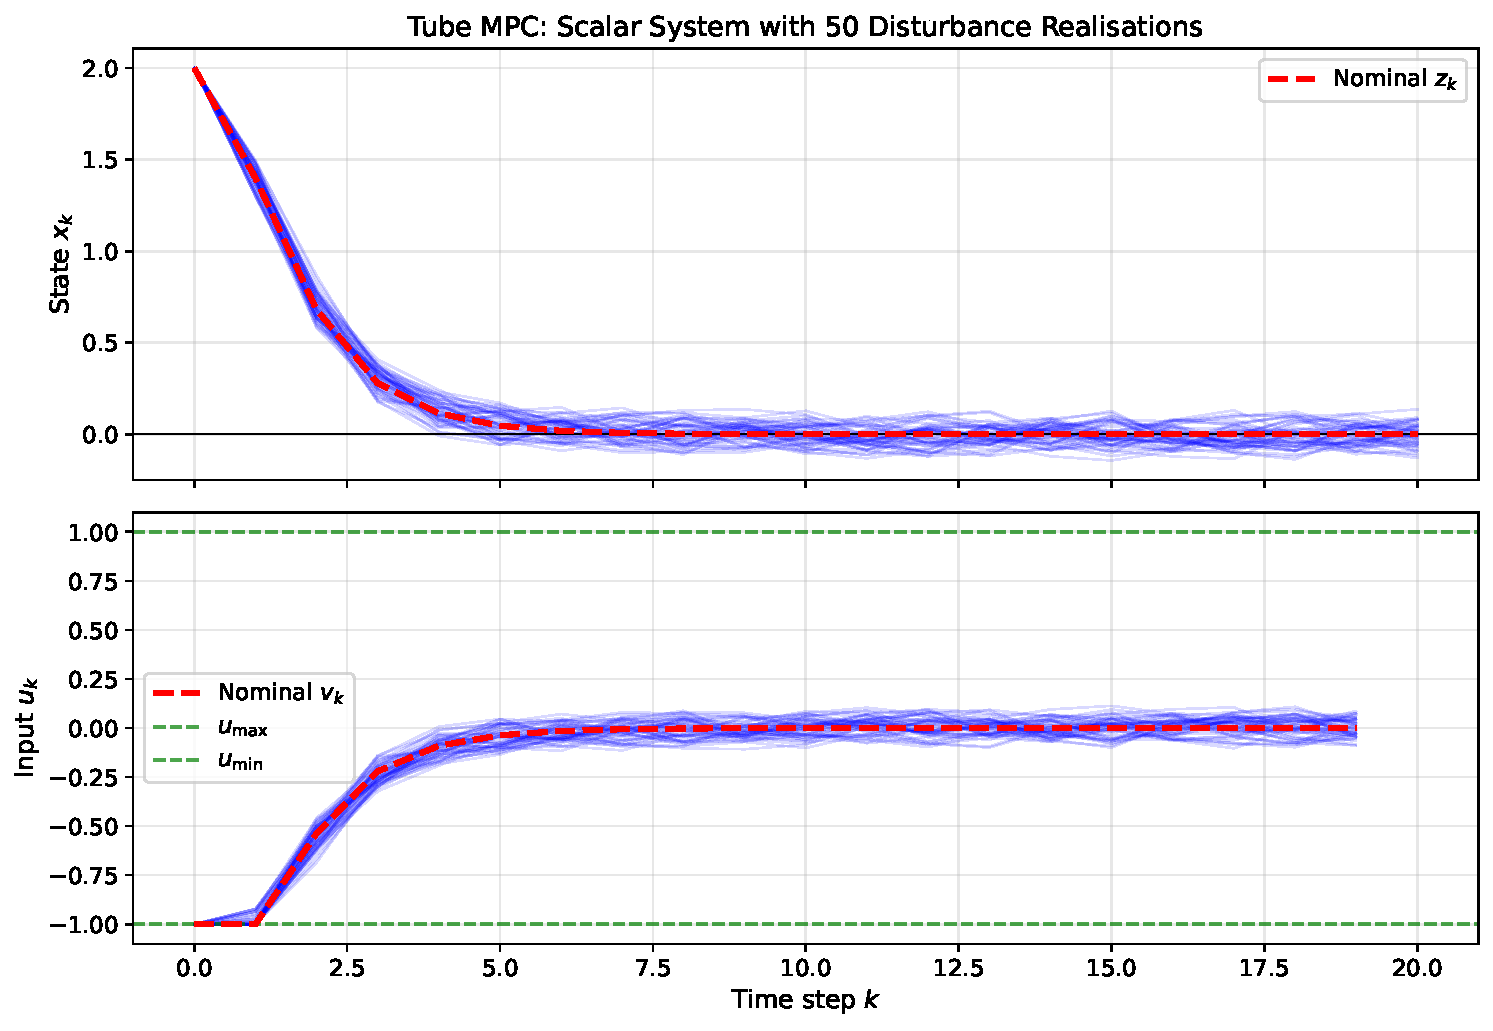
\includegraphics[width=0.85\linewidth]{Figures/tube_mpc_scalar.pdf}
	\caption{Tube MPC applied to the scalar system $x_{k+1} = 1.2\,x_k + u_k + w_k$ with $|w_k| \le 0.1$. Fifty disturbance realisations (blue) cluster around the nominal trajectory (red dashed). All trajectories satisfy the input constraints $|u_k| \le 1$.}
	\label{fig:tube_scalar}
\end{figure}


\section{Worked Example: Two-State System}
\label{sec:tube_example_2d}

\begin{examplebox}{Tube MPC: Double Integrator with Disturbance}
	Consider the double integrator:
	\[
	A = \begin{bmatrix} 1 & 1 \\ 0 & 1 \end{bmatrix}, \quad B = \begin{bmatrix} 0.5 \\ 1 \end{bmatrix}, \quad w_k \in \mathcal{W} = \{w \mid \|w\|_\infty \le 0.05\}
	\]
	with $|u_k| \le 1$, $|x_{1,k}| \le 5$, $|x_{2,k}| \le 3$, and $Q = I_2$, $R = 1$.

	\solution

	\textbf{Step 1: Compute LQR gain.}

	Solving the DARE gives $K = [0.4345 \;\; 1.0285]$ (positive, as returned by \texttt{dlqr}) and $P = \begin{bmatrix} 2.3671 & 1.1180 \\ 1.1180 & 2.5875 \end{bmatrix}$.

	The closed-loop matrix is:
	\[
	A_{cl} = A - BK = \begin{bmatrix} 1 - 0.2172 & 1 - 0.5142 \\ 0 - 0.4345 & 1 - 1.0285 \end{bmatrix} = \begin{bmatrix} 0.7828 & 0.4858 \\ -0.4345 & -0.0285 \end{bmatrix}
	\]
	The eigenvalues of $A_{cl}$ are approximately $0.377 \pm 0.216j$, with $|\lambda| \approx 0.434$, well inside the unit circle.

	\textbf{Step 2: Compute the mRPI set $\mathcal{E}$.}

	This requires the iterative Minkowski sum~\eqref{eq:mrpi}. For a two-state system, this is not practical by hand. Using MPT3 in MATLAB:

\begin{lstlisting}[language=Matlab]
A = [1 1; 0 1]; B = [0.5; 1];
Q = eye(2); R = 1;
[K_lqr, ~] = dlqr(A, B, Q, R);
Acl = A - B*K_lqr;

% Disturbance set
W = Polyhedron('lb', [-0.05; -0.05], 'ub', [0.05; 0.05]);

% Compute mRPI set (iterative Minkowski sum approximation)
% Note: invariantSet() computes the MAXIMAL positive invariant set,
% which is NOT the mRPI. The mRPI is computed via the iteration below.
Omega = W;
for i = 1:30
    Omega_new = Omega + (Acl^i) * W;  % Minkowski sum
    if Omega_new == Omega              % convergence check
        fprintf('mRPI converged at iteration %d\n', i);
        break;
    end
    Omega = Omega_new;
end
E = Omega;
\end{lstlisting}

	\textbf{Step 3: Tighten constraints.}
\begin{lstlisting}[language=Matlab]
X = Polyhedron('lb', [-5; -3], 'ub', [5; 3]);
U = Polyhedron('lb', -1, 'ub', 1);
KE = K_lqr * E;           % Image of E under K (set of |Ke| values)

Xt = X - E;               % Pontryagin difference
Vt = U - KE;              % Pontryagin difference
\end{lstlisting}

	\textbf{Step 4: Solve nominal MPC with tightened constraints.}

	The optimisation~\eqref{eq:tube_mpc_opt} is a standard QP with the same structure as Chapter~7. The only difference is that $\mathcal{X}$, $\mathcal{U}$ are replaced by $\mathcal{X}_t$, $\mathcal{V}$.

	\textbf{Step 5: Apply.} $u_k = v_0^\star - K(x_k - z_0^\star)$.
\end{examplebox}


\section{Guarantees of Tube MPC}
\label{sec:tube_guarantees}

Tube MPC provides three key guarantees, under the same type of assumptions as the nominal MPC stability theory (Chapter~7, Section~\ref{sec:mpc_stability_theory}).

\begin{summarybox}{Theorem: Properties of Tube MPC}
	Suppose $(A, B)$ is stabilisable, $K$ is chosen so that $A_{cl} = A - BK$ is Schur stable, and the MPC formulation~\eqref{eq:tube_mpc_opt} includes a terminal cost $P$ (DARE solution) and terminal set $\mathcal{X}_f$ for the nominal system. Then, for any disturbance sequence $\{w_k\} \subseteq \mathcal{W}$:
	\begin{enumerate}[noitemsep]
		\item \textbf{Robust constraint satisfaction:} The actual state and input satisfy $x_k \in \mathcal{X}$ and $u_k \in \mathcal{U}$ for all $k \ge 0$.
		\item \textbf{Recursive feasibility:} If the optimisation~\eqref{eq:tube_mpc_opt} is feasible at $k = 0$, it is feasible for all $k \ge 0$.
		\item \textbf{Robust stability:} The actual state converges to a neighbourhood of the origin. Specifically, $x_k$ converges to the mRPI set $\mathcal{E}$ (not to the origin itself, because the persistent disturbance prevents exact convergence).
	\end{enumerate}
\end{summarybox}

The first property follows directly from constraint tightening. The second uses the same shifted-sequence argument as in Chapter~7, applied to the nominal system. The third uses the nominal optimal cost $J^\star(z)$ as a Lyapunov function for the nominal system and then bounds the deviation of the real state.

Note a subtle difference from the nominal case: the state does not converge to zero. It converges to the mRPI set $\mathcal{E}$ around the origin. This is the best we can hope for with persistent disturbances --- we cannot drive the state to exactly zero when the disturbance keeps pushing it around.


\section{Tube MPC vs Standard MPC: A Comparison}
\label{sec:tube_comparison}

\begin{center}
	\begin{tabular}{L{4cm} C{4.5cm} C{4.5cm}}
		\toprule
		& \textbf{Standard MPC} & \textbf{Tube MPC} \\
		\midrule
		Model & $x_{k+1} = Ax_k + Bu_k$ & $x_{k+1} = Ax_k + Bu_k + w_k$ \\[3pt]
		Disturbance & Ignored & Bounded: $w_k \in \mathcal{W}$ \\[3pt]
		Constraint guarantee & Nominal only & Robust (for all $w \in \mathcal{W}$) \\[3pt]
		Online computation & Solve QP & Solve QP (same size) + feedback \\[3pt]
		Offline computation & $P$, $K$, $\mathcal{X}_f$ & $P$, $K$, $\mathcal{E}$, $\mathcal{X}_t$, $\mathcal{V}$, $\mathcal{X}_f$ \\[3pt]
		Convergence & $x_k \to 0$ & $x_k \to \mathcal{E}$ (neighbourhood of 0) \\[3pt]
		Feasible region & Larger & Smaller (due to tightening) \\
		\bottomrule
	\end{tabular}
\end{center}

The main takeaway: Tube MPC achieves robust guarantees at essentially no additional online cost. The extra work is in the offline design (computing $\mathcal{E}$ and tightening constraints), not in the real-time optimisation. The QP solved at each step has exactly the same size and structure as standard MPC.


\section{Implementation in MATLAB}
\label{sec:tube_matlab}

The following MATLAB code implements a complete Tube MPC simulation for the scalar system from Section~\ref{sec:tube_example_scalar}, using YALMIP.

\begin{lstlisting}[language=Matlab, caption={Tube MPC implementation for the scalar system}]
%% Tube MPC: Scalar System
% x_{k+1} = 1.2*x_k + u_k + w_k,  |w_k| <= 0.1
clear; clc;

%--- System parameters ---
a = 1.2;  b = 1;
Q = 1;    R = 1;    N = 5;

%--- Constraints ---
x_max = 5;   u_max = 1;   w_max = 0.1;

%--- Step 1: LQR gain ---
[K_lqr, P_dare] = dlqr(a, b, Q, R);
K = K_lqr;         % K > 0 (dlqr convention); control law: u = -K*x
a_cl = a - b*K;    % closed-loop eigenvalue: a_cl = a - b*K
fprintf('K = %.4f, a_cl = %.4f\n', K, a_cl);

%--- Step 2: mRPI set (scalar: geometric series) ---
e_bar = w_max / (1 - abs(a_cl));
fprintf('mRPI half-width: e_bar = %.4f\n', e_bar);

%--- Step 3: Tighten constraints ---
x_max_t = x_max - e_bar;              % tightened state
u_max_t = u_max - abs(K) * e_bar;     % tightened input
fprintf('Tightened: |z| <= %.3f, |v| <= %.3f\n', x_max_t, u_max_t);

%--- Step 4: Build nominal MPC with YALMIP ---
% z(1) is a decision variable (optimised), not fixed to x(k).
% Constraint: |x(k) - z(1)| <= e_bar (i.e., x(k) in {z(1)} + E).
z = sdpvar(1, N+1);   % nominal states (z(1) = z_0 is optimised)
v = sdpvar(1, N);      % nominal inputs
x_meas = sdpvar(1);   % parameter: measured state

constraints = [];
cost = 0;
for i = 1:N
    cost = cost + z(i)^2 * Q + v(i)^2 * R;
    constraints = [constraints, ...
        z(i+1) == a*z(i) + b*v(i), ...
        -x_max_t <= z(i) <= x_max_t, ...
        -u_max_t <= v(i) <= u_max_t];
end
cost = cost + z(N+1)^2 * P_dare;  % terminal cost
constraints = [constraints, -x_max_t <= z(N+1) <= x_max_t];

% Tube constraint: x(k) must lie in {z_0} + E
constraints = [constraints, -e_bar <= x_meas - z(1) <= e_bar];

params_in = x_meas;          % parameter: measured state
sols_out = [v(1), z(1)];     % solutions: first nominal input AND z_0

ops = sdpsettings('verbose', 0, 'solver', 'quadprog');
controller = optimizer(constraints, cost, ops, params_in, sols_out);

%--- Step 5: Simulate ---
T_sim = 30;
x = zeros(1, T_sim+1);
z_traj = zeros(1, T_sim+1);
u_applied = zeros(1, T_sim);

x(1) = 2.0;      % initial condition

rng(42);
for k = 1:T_sim
    % Solve nominal MPC (z_0 is optimised, not fixed to x(k))
    sol = controller(x(k));
    v0 = sol(1);
    z0 = sol(2);

    % Apply tube control law: u = v - K*(x - z)
    % Note: z0 ~= x(k) in general, so the feedback term is nonzero
    u_applied(k) = v0 - K * (x(k) - z0);
    u_applied(k) = max(-u_max, min(u_max, u_applied(k)));

    % Simulate real system with disturbance
    w = w_max * (2*rand - 1);   % uniform in [-w_max, w_max]
    x(k+1) = a * x(k) + b * u_applied(k) + w;

    % Store nominal trajectory for plotting
    z_traj(k) = z0;
    z_traj(k+1) = a * z0 + b * v0;
end

%--- Plot ---
figure;
subplot(2,1,1);
plot(0:T_sim, x, 'b-', 'LineWidth', 1.5); hold on;
plot(0:T_sim, z_traj, 'r--', 'LineWidth', 1.5);
yline(x_max, 'g--'); yline(-x_max, 'g--');
ylabel('State'); legend('Actual x_k', 'Nominal z_k', 'Constraint');
title('Tube MPC: Scalar System'); grid on;

subplot(2,1,2);
stairs(0:T_sim-1, u_applied, 'b-', 'LineWidth', 1.5);
yline(u_max, 'g--'); yline(-u_max, 'g--');
xlabel('Time step k'); ylabel('Input u_k');
legend('Applied input', 'Constraint'); grid on;
\end{lstlisting}


\section{Computing the mRPI Set with MPT3}
\label{sec:tube_mpt3}

For multi-state systems, computing the mRPI set by hand is impractical. The MPT3 toolbox~\cite{Herceg2013} provides automated tools for this. The key steps are:

\begin{lstlisting}[language=Matlab, caption={Computing the mRPI set and tightened constraints using MPT3}]
%% Tube MPC Offline Design using MPT3
% System: x+ = Ax + Bu + w,  w in W

A = [1 1; 0 1];   B = [0.5; 1];
Q = eye(2);        R = 1;

% LQR gain
[K_lqr, P_dare] = dlqr(A, B, Q, R);
Acl = A - B*K_lqr;

% Define constraint sets as Polyhedra
X = Polyhedron('lb', [-5; -3], 'ub', [5; 3]);     % state
U = Polyhedron('lb', -1, 'ub', 1);                 % input
W = Polyhedron('lb', [-0.05; -0.05], ...
               'ub', [0.05; 0.05]);                 % disturbance

% --- Compute the mRPI set ---
% Iterative Minkowski sum: E = W + Acl*W + Acl^2*W + ...
E = W;
for i = 1:30
    E_new = E + Acl^i * W;   % Minkowski sum
    if E_new == E             % convergence check
        fprintf('mRPI converged at iteration %d\n', i);
        break;
    end
    E = E_new;
end
\end{lstlisting}

\begin{notebox}{Convergence check}
The equality test \texttt{E\_new == E} uses MPT3's polytope comparison, which involves solving linear programmes.  For production code, a tolerance-based criterion (e.g.\ comparing support functions or Hausdorff distances) is more numerically robust.  The outer-approximation algorithm of \citet{Rakovic2005} provides explicit error bounds.
\end{notebox}

\begin{lstlisting}[language=Matlab]

% --- Tighten constraints ---
KE  = K_lqr * E;        % image of E under gain K (set of |Ke| values)
Xt  = X - E;             % Pontryagin difference: X ominus E
Vt  = U - KE;            % Pontryagin difference: U ominus KE

% --- Compute terminal set for nominal system ---
sys_nom = LTISystem('A', A - B*K_lqr);
% NOTE: Xt.Internal.lb/ub exist because X and E are both boxes (hyperrectangles).
% For general polytopic constraints, use Xt.A and Xt.b with LTISystem's setConstraint method.
sys_nom.x.min = Xt.Internal.lb;
sys_nom.x.max = Xt.Internal.ub;
Xf = sys_nom.invariantSet();

% --- Extract half-space representation for QP ---
% Tightened state: Xt.A * z <= Xt.b
% Tightened input: Vt.A * v <= Vt.b
% Terminal:        Xf.A * z_N <= Xf.b

fprintf('Tightened state constraints: %d inequalities\n', size(Xt.A, 1));
fprintf('Tightened input constraints: %d inequalities\n', size(Vt.A, 1));
fprintf('Terminal set: %d inequalities\n', size(Xf.A, 1));
\end{lstlisting}

\begin{notebox}{Approximate mRPI for large systems}
	For systems with more than 3--4 states, the exact mRPI computation can produce polytopes with a very large number of faces, making the resulting QP expensive. In practice, an outer approximation $\hat{\mathcal{E}} \supseteq \mathcal{E}_\infty$ is often used instead~\cite{Rakovic2005}. A common approach is to stop the iteration after a fixed number of steps $s$ and scale the result slightly outward: $\hat{\mathcal{E}} = (1-\epsilon)^{-1}\,\Omega_s$ for a small $\epsilon > 0$ chosen so that $A_{cl}^{s+1}\mathcal{W} \subseteq \epsilon\,\Omega_s$. This guarantees that $\hat{\mathcal{E}}$ is a true RPI set while keeping the number of polytope faces manageable.
\end{notebox}


\section{Visualising the Tube}
\label{sec:tube_visualisation}

Figure~\ref{fig:tube_concept} illustrates the key concept. The nominal trajectory $z_k$ (red dashed) is planned by the MPC optimiser. The actual trajectory $x_k$ (blue solid) deviates due to disturbances but stays within the grey ``tube'' --- the Minkowski sum $\{z_k\} \oplus \mathcal{E}$ at each step. The nominal trajectory respects the tightened constraints (orange lines), which guarantees the actual trajectory respects the original constraints (green dashed lines).

\begin{figure}[H]
	\centering
	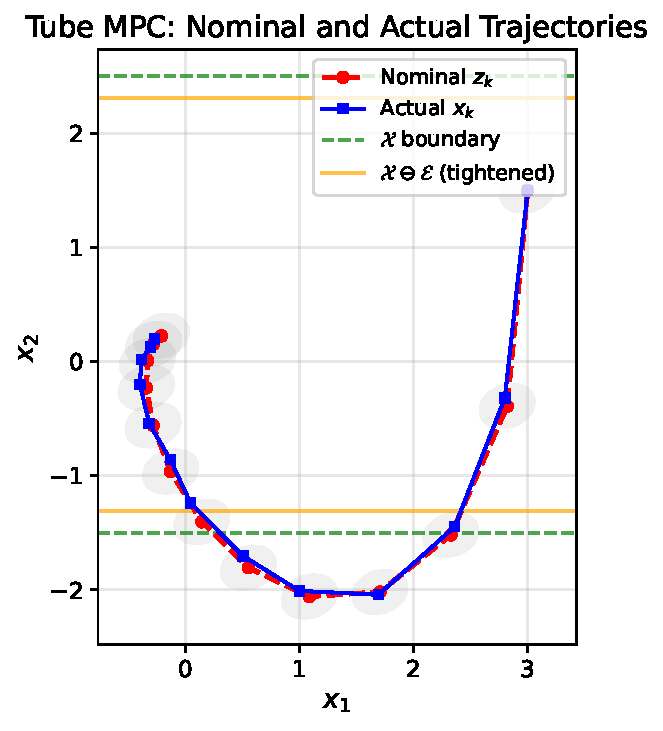
\includegraphics[width=0.85\linewidth]{Figures/tube_mpc_concept.pdf}
	\caption{The tube concept in state space. Grey ellipses represent the cross-section $\mathcal{E}$ of the tube at each time step. The nominal trajectory (red) stays within the tightened constraints (orange), ensuring the actual trajectory (blue) stays within the original constraints (green dashed).}
	\label{fig:tube_concept}
\end{figure}


\section{Summary and Practical Guidelines}

\begin{summarybox}{Tube MPC Design Recipe}
	\begin{enumerate}
		\item \textbf{Model the disturbance.} Identify the disturbance set $\mathcal{W}$ from physical knowledge or data. Larger $\mathcal{W}$ gives more robustness but tighter constraints.

		\item \textbf{Choose the feedback gain $K$.} Use LQR or pole placement. Faster gains give a smaller tube (less constraint tightening) but require more control effort (more input constraint tightening). There is a design trade-off.

		\item \textbf{Compute the mRPI set $\mathcal{E}$.} Use the iterative Minkowski sum~\eqref{eq:mrpi} or MPT3. For scalar systems, use the geometric series formula.

		\item \textbf{Tighten constraints.} State: $\mathcal{X}_t = \mathcal{X} \ominus \mathcal{E}$. Input: $\mathcal{V} = \mathcal{U} \ominus K\mathcal{E}$. Check that the tightened sets are non-empty; if they are empty, the disturbance is too large relative to the constraints, and robust constraint satisfaction is impossible.

		\item \textbf{Design the nominal MPC.} Solve a standard MPC problem with the tightened constraints. All the techniques from Chapter~7 apply (terminal cost $P$, terminal set $\mathcal{X}_f$, YALMIP implementation).

		\item \textbf{Apply the tube law.} At each step: $u_k = v_0^\star - K(x_k - z_0^\star)$.
	\end{enumerate}
\end{summarybox}

\begin{alertbox}{When Tube MPC cannot help}
	If the disturbance bound $\mathcal{W}$ is so large that the tightened constraint sets $\mathcal{X}_t$ or $\mathcal{V}$ become empty, then no controller can guarantee robust constraint satisfaction. In this case, the system physically cannot respect the constraints under all possible disturbances. Options include: relaxing the constraints (soft constraints), reducing the disturbance (better actuators or shielding), or accepting occasional constraint violations and using a stochastic MPC approach instead.
\end{alertbox}


\section*{Further Reading}

The Tube MPC framework was introduced by Langson et al.~\cite{Langson2004} and further
developed by Mayne et al.~\cite{Mayne2005}. The efficient outer approximation of the
mRPI set used in practice is due to Rakovi{\'c} et al.~\cite{Rakovic2005}. For a
comprehensive treatment of robust MPC including stochastic formulations, see
Kouvaritakis and Cannon~\cite{Kouvaritakis2016}. The broader MPC stability theory
underpinning the guarantees discussed in this chapter is surveyed in
Mayne et al.~\cite{Mayne2000}. The textbooks by Rawlings et al.~\cite{Rawlings2017}
and Borrelli et al.~\cite{Borrelli2017} provide detailed treatments of both nominal
and robust MPC.

\section*{Exercises}
\begin{enumerate}

	\item Consider the scalar system $x_{k+1} = 1.5\,x_k + u_k + w_k$ with $|u_k| \le 2$, $|w_k| \le 0.2$, and $Q = R = 1$.
	\begin{enumerate}
		\item Compute the LQR gain $K$ and the closed-loop eigenvalue $a_{cl}$.
		\item Using the geometric series formula, compute the mRPI half-width $\bar{e}$.
		\item What are the tightened input constraints for the nominal MPC?
		\item If $|x_k| \le 10$, what are the tightened state constraints?
	\end{enumerate}

	\item Compute the Minkowski sum $P \oplus Q$ and the Pontryagin difference $P \ominus Q$ for:
	\begin{enumerate}
		\item $P = [-3, 3]$, $Q = [-1, 1]$ (intervals in $\mathbb{R}$).
		\item $P = \{(x_1, x_2) \mid |x_1| \le 2, |x_2| \le 2\}$ (a square) and $Q = \{(x_1, x_2) \mid |x_1| + |x_2| \le 0.5\}$ (a diamond). Sketch the results.
	\end{enumerate}

	\item A control engineer designs Tube MPC for a chemical process with $|w_k| \le 0.5$ and input constraint $|u_k| \le 3$. The LQR gain is $K = 1.8$ (positive, with $u = -Kx$) and the closed-loop eigenvalue is $a_{cl} = 0.3$.
	\begin{enumerate}
		\item Compute the tube width $\bar{e}$.
		\item What is the tightened input constraint for $v_k$?
		\item The engineer's colleague suggests using a more aggressive gain with $a_{cl} = 0.1$, which gives $K = 2.5$. Recompute the tube width and tightened input constraint. Is this gain better or worse? Discuss the trade-off.
	\end{enumerate}

	\item Consider the double integrator from Section~\ref{sec:tube_example_2d}. Using MATLAB and MPT3:
	\begin{enumerate}
		\item Compute the mRPI set $\mathcal{E}$ for $\mathcal{W} = \{w \mid \|w\|_\infty \le 0.05\}$.
		\item Plot the original constraint set $\mathcal{X}$, the mRPI set $\mathcal{E}$, and the tightened constraint set $\mathcal{X}_t = \mathcal{X} \ominus \mathcal{E}$.
		\item Repeat with $\mathcal{W} = \{w \mid \|w\|_\infty \le 0.2\}$. How does the larger disturbance affect the feasible region?
		\item Find the largest disturbance bound $\delta$ such that $\mathcal{X}_t$ is still non-empty (i.e., the tightened constraint set has positive volume).
	\end{enumerate}

	\item Explain in your own words:
	\begin{enumerate}
		\item Why does Tube MPC guarantee convergence to a neighbourhood of the origin rather than to the origin itself?
		\item What happens to the tube width $\mathcal{E}$ as the feedback gain $K$ becomes more aggressive (eigenvalues of $A_{cl}$ closer to zero)?
		\item Under what conditions does Tube MPC reduce to standard MPC?
	\end{enumerate}

\end{enumerate}

	\chapter{Nonlinear Model Predictive Control\texorpdfstring{$^{(*)}$}{(*)}}
\label{chap:nmpc}

\begin{quote}
	\textit{``The real world is nonlinear.''} \\
	\hfill --- virtually every control textbook
\end{quote}

Linear MPC assumes $x_{k+1} = Ax_k + Bu_k$. This is adequate near a single operating point, but fails when the system traverses large regions of its state space. A pendulum cannot swing from hanging to inverted using a controller designed around either equilibrium. A rocket cannot land using a model linearised at altitude. A chemical reactor cannot transition between steady states through a linear corridor.

This chapter develops Nonlinear MPC (NMPC), which replaces the linear model with the full nonlinear dynamics $x_{k+1} = f(x_k, u_k)$. Two solution paradigms are presented:
\begin{enumerate}[nosep]
	\item \textbf{Nonlinear programming (NLP):} Solve the non-convex optimisation directly using interior-point or SQP methods (Section~\ref{sec:nmpc_nlp}).
	\item \textbf{Sequential convex programming (SCP):} Approximate the NLP as a sequence of QPs, each solved with the fast, reliable tools from Chapter~\ref{chap:linear_mpc} (Section~\ref{sec:scp}).
\end{enumerate}
Both approaches are demonstrated on physical systems: a pendulum swing-up (NLP) and a powered rocket landing (SCP).


% ================================================================
% THE NONLINEAR OCP
% ================================================================
\section{The Nonlinear Optimal Control Problem}
\label{sec:nmpc_ocp}

At each sampling instant $t$, NMPC solves the following optimal control problem (OCP):

\begin{defnbox}{The NMPC Optimisation Problem}
	\begin{align*}
		\min_{u_0, \dots, u_{N-1}} \quad & J = \sum_{k=0}^{N-1} \ell(x_k, u_k) + V_f(x_N) \\[4pt]
		\text{s.t.} \quad
		& x_0 = x(t) & \text{(Initialisation)} \\
		& x_{k+1} = f(x_k, u_k), \;\; k = 0, \dots, N{-}1 & \text{(Nonlinear Dynamics)} \\
		& h(x_k, u_k) \le 0, \;\; k = 0, \dots, N{-}1 & \text{(Path Constraints)} \\
		& x_N \in \mathcal{X}_f & \text{(Terminal Constraint)}
	\end{align*}
	where $\ell(\cdot)$ is the stage cost, $V_f(\cdot)$ the terminal cost, $f(\cdot)$ the nonlinear discrete-time dynamics, $h(\cdot)$ encodes state and input constraints, and $\mathcal{X}_f$ is the terminal set.
\end{defnbox}

When $f$ is linear and $\ell$, $V_f$ are quadratic, this reduces to the QP of Chapter~\ref{chap:linear_mpc}. For general $f$, the equality constraints $x_{k+1} = f(x_k, u_k)$ make the feasible set non-convex, and the problem becomes a \emph{nonlinear programme (NLP)}.

Two consequences follow:
\begin{itemize}[nosep]
	\item \textbf{Local minima.} Solvers may converge to a locally optimal but globally suboptimal solution. The result depends on the initial guess.
	\item \textbf{Computational cost.} Each NLP iteration requires Jacobians and possibly Hessians of $f$ and $h$. The solver must finish within one sampling period $T_s$.
\end{itemize}

\begin{notebox}{NMPC Reduces to Linear MPC}
	Setting $f(x,u) = Ax + Bu$, $\ell(x,u) = x^\top Q x + u^\top R u$, $V_f(x) = x^\top P x$, and $h(x,u) = [u - u_{\max};\; -u + u_{\min};\; x - x_{\max};\; -x + x_{\min}]$ recovers the QP from Section~\ref{sec:mpc_formulation} exactly. Every result in this chapter specialises to the linear case.
\end{notebox}

\textbf{Stability.} The stability framework from Chapter~\ref{chap:linear_mpc} (terminal cost, terminal set, recursive feasibility) extends to NMPC, but proving it requires stronger assumptions: the terminal cost $V_f$ must be a local control Lyapunov function for the nonlinear dynamics, and the terminal set $\mathcal{X}_f$ must be positively invariant under a local stabilising controller. The seminal reference is~\cite{Mayne2000}; a textbook treatment is given in~\cite{Grune2017}. In this chapter, we focus on computation rather than stability proofs.

% ================================================================
% DIRECT TRANSCRIPTION
% ================================================================
\section{Direct Transcription Methods}
\label{sec:direct_transcription}

The OCP is an infinite-dimensional problem (optimise over function spaces). \emph{Direct methods} discretise time and convert it into a finite-dimensional NLP that standard solvers can handle.

\subsection{Direct Single Shooting}

Eliminate the states entirely. Given a control sequence $u_0, \dots, u_{N-1}$ and the initial state $x_0$, simulate forward:
\[
x_1 = f(x_0, u_0), \quad x_2 = f(x_1, u_1), \quad \dots, \quad x_N = f(x_{N-1}, u_{N-1}).
\]
The NLP has $N \cdot n_u$ decision variables (controls only). State constraints must be imposed as functions of $(u_0, \dots, u_{N-1})$, which couples all variables and produces dense Jacobians.

Single shooting is simple to implement but suffers from ill-conditioning: a small change in $u_0$ propagates through the entire trajectory, producing steep, poorly scaled gradients.

\subsection{Direct Multiple Shooting}

Treat both states and controls as decision variables. The dynamics become explicit equality constraints:

\begin{defnbox}{Direct Multiple Shooting NLP}
	Decision variables: $z = (x_1, \dots, x_N, u_0, \dots, u_{N-1}) \in \mathbb{R}^{N(n_x + n_u)}$.
	\begin{align*}
		\min_z \quad & \sum_{k=0}^{N-1} \ell(x_k, u_k) + V_f(x_N) \\
		\text{s.t.} \quad & x_{k+1} - f(x_k, u_k) = 0, \quad k = 0, \dots, N{-}1 \\
		& h(x_k, u_k) \le 0, \quad k = 0, \dots, N{-}1 \\
		& x_0 = x(t) \;\text{(fixed)}
	\end{align*}
\end{defnbox}

The problem is larger ($N(n_x + n_u)$ variables vs.\ $N n_u$), but the constraint Jacobian is \emph{block-banded}: the dynamics at step $k$ involve only $(x_k, u_k, x_{k+1})$. NLP solvers exploit this sparsity for $O(N)$ per-iteration cost.

Multiple shooting also decouples the trajectory: perturbations in $u_k$ affect $x_{k+1}$ directly but do not cascade further (the equality constraints absorb the mismatch). This dramatically improves convergence compared to single shooting.

\begin{alertbox}{Which Transcription to Use?}
	Direct multiple shooting is the default choice for NMPC. It offers better convergence, straightforward state constraints, and exploitable sparsity. Single shooting is only competitive for very small problems ($N \cdot n_u < 10$) or when the dynamics are cheap to simulate but expensive to differentiate.
\end{alertbox}

\subsection{Direct Collocation (Brief)}

Instead of Forward Euler or RK4 integration between shooting nodes, \emph{direct collocation} approximates the state trajectory within each interval by a polynomial (typically Legendre or Radau). The polynomial coefficients become decision variables, and the dynamics are enforced at selected collocation points.

Collocation produces an implicit integration scheme, making it well-suited for stiff systems (chemical reactors, power electronics). The NLP is larger but highly structured. We do not develop collocation further here; see \cite{Rawlings2017} for a detailed treatment.


% ================================================================
% NMPC VIA NLP
% ================================================================
\section{NMPC via Nonlinear Programming}
\label{sec:nmpc_nlp}

\subsection{CasADi and IPOPT}

\emph{CasADi}~\cite{Andersson2019} is an open-source framework for algorithmic differentiation (AD) and numerical optimisation. It provides a symbolic interface for defining nonlinear functions and automatically generates the exact Jacobians and Hessians required by NLP solvers. CasADi interfaces with \emph{IPOPT} (Interior Point OPTimiser), a primal-dual interior-point solver for large-scale NLPs.

The workflow in MATLAB is:
\begin{enumerate}[nosep]
	\item Declare symbolic variables via \texttt{casadi.Opti()}.
	\item Define dynamics, cost, and constraints symbolically.
	\item Call \texttt{opti.solver('ipopt')} and \texttt{opti.solve()}.
\end{enumerate}
CasADi computes all derivatives automatically---no manual Jacobians required.

\subsection{Worked Example: Pendulum Swing-Up}

\begin{examplebox}{NMPC for Pendulum Swing-Up}
	A simple pendulum of mass $m$ and length $l$ is actuated by a torque $\tau$ at the pivot. The angle $\theta$ is measured from the \emph{upright} vertical ($\theta = 0$ is inverted, $\theta = \pi$ is hanging). The continuous-time dynamics are:
	\begin{align*}
		\dot{\theta} &= \omega, &
		\dot{\omega} &= \frac{g}{l}\sin\theta + \frac{\tau}{m l^2},
	\end{align*}
	where $g = 9.81\;\text{m/s}^2$, $l = 1\;\text{m}$, $m = 1\;\text{kg}$, and $|\tau| \le 5\;\text{N\,m}$.

	\textbf{Task:} Drive the pendulum from the stable hanging position $(\theta, \omega) = (\pi, 0)$ to the unstable upright equilibrium $(\theta, \omega) = (0, 0)$ --- the classic \emph{swing-up} manoeuvre.

	\solution

	Linear MPC linearised at the upright equilibrium gives $\dot{\omega} \approx (g/l)\theta + \tau/(ml^2)$. Near $\theta = 0$ this is a valid model, but at $\theta = \pi$ the linearisation predicts $\dot{\omega} \approx (g/l)\pi + \tau/(ml^2)$, which is qualitatively wrong (the gravitational torque has the wrong sign). A linear controller designed around the upright position has no mechanism to swing the pendulum up from below.

	NMPC uses the full nonlinear model and can plan the energy-pumping trajectory needed for the swing-up. The receding-horizon NMPC controller solves the following NLP at each time step:
	\begin{align*}
		\min_{u_0, \dots, u_{N-1}} \quad & \sum_{k=0}^{N-1} (x_k^\top Q\, x_k + R\, u_k^2) + x_N^\top P\, x_N \\
		\text{s.t.} \quad & x_{k+1} = \text{RK4}(x_k, u_k, T_s), \quad |u_k| \le 5,
	\end{align*}
	with $x = [\theta, \omega]^\top$, $Q = \operatorname{diag}(50, 0.1)$, $R = 0.1$, $P = \operatorname{diag}(1000, 10)$, $N = 40$, $T_s = 0.05$\,s.
\end{examplebox}

The RK4 integrator for one time step is:
\[
\text{RK4}(x, u, h) = x + \tfrac{h}{6}(k_1 + 2k_2 + 2k_3 + k_4),
\]
where $k_1 = f(x, u)$, $k_2 = f(x + \tfrac{h}{2}k_1, u)$, $k_3 = f(x + \tfrac{h}{2}k_2, u)$, $k_4 = f(x + h\,k_3, u)$.

\begin{lstlisting}[language=Matlab, caption={Pendulum swing-up NMPC using CasADi and IPOPT.}, label=lst:casadi_pendulum]
import casadi.*
opti = casadi.Opti();

% Parameters
g_val = 9.81; L = 1; m_val = 1;
N = 40; dt = 0.05; tau_max = 5;
Q = diag([50, 0.1]); R_w = 0.1; P_w = diag([1000, 10]);

% Symbolic variables
X = opti.variable(2, N+1);  U = opti.variable(1, N);
x_init = opti.parameter(2, 1);

% Continuous dynamics
f_cont = @(x, u) [x(2); (g_val/L)*sin(x(1)) + u/(m_val*L^2)];

% RK4 integrator
rk4 = @(x, u, h) rk4_step(x, u, h, f_cont);

% Constraints and cost
opti.subject_to(X(:,1) == x_init);
J = 0;
for k = 1:N
    opti.subject_to(X(:,k+1) == rk4(X(:,k), U(k), dt));
    opti.subject_to(-tau_max <= U(k) <= tau_max);
    J = J + X(:,k)'*Q*X(:,k) + R_w*U(k)^2;
end
J = J + X(:,N+1)'*P_w*X(:,N+1);
opti.minimize(J);
opti.solver('ipopt', struct('expand',true), ...
            struct('max_iter',2000, 'print_level',0));

% Receding-horizon simulation
T_sim = 200; x_curr = [pi; 0];
x_hist = zeros(2, T_sim+1); x_hist(:,1) = x_curr;
u_hist = zeros(1, T_sim);

for t = 1:T_sim
    opti.set_value(x_init, x_curr);
    sol = opti.solve();
    u_val = full(sol.value(U(1)));
    x_curr = full(rk4(x_curr, u_val, dt));
    x_hist(:,t+1) = x_curr;  u_hist(t) = u_val;
    opti.set_initial(X, sol.value(X));    % warm-start
    opti.set_initial(U, sol.value(U));
end

function xn = rk4_step(x, u, h, f)
    k1 = f(x,u); k2 = f(x+h/2*k1,u);
    k3 = f(x+h/2*k2,u); k4 = f(x+h*k3,u);
    xn = x + (h/6)*(k1+2*k2+2*k3+k4);
end
\end{lstlisting}

Figure~\ref{fig:nmpc_pendulum} shows the result. The controller swings the pendulum through the lower equilibrium, building kinetic energy, then catches it at the inverted position. The torque saturates at $\pm 5$\,N\,m during the energy-pumping phase and decays to zero once the pendulum is balanced. This trajectory is impossible for any linear controller designed around a single equilibrium.

\begin{figure}[ht]
	\centering
	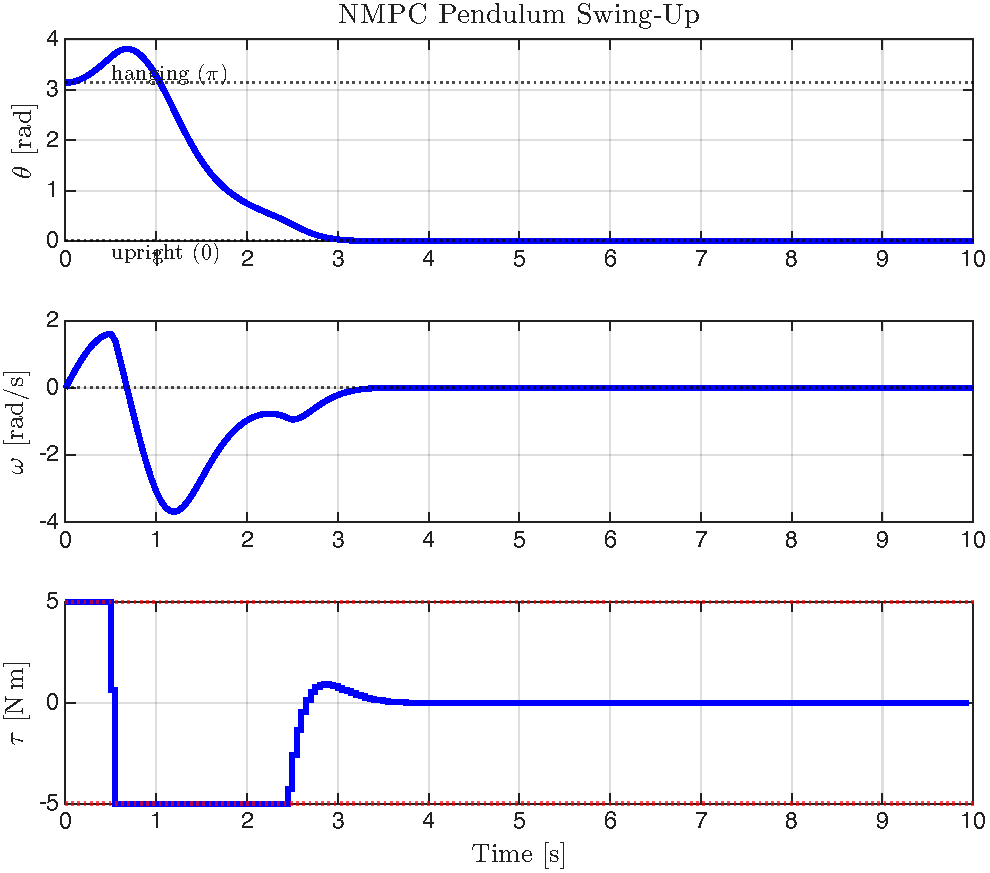
\includegraphics[width=0.85\textwidth]{Figures/fig_nmpc_pendulum_swingup.pdf}
	\caption{NMPC pendulum swing-up. Top: angle $\theta$ from the upright position ($\theta = \pi$ is hanging, $\theta = 0$ is inverted). The controller pumps energy by swinging through the lower equilibrium before catching the pendulum at the top. Middle: angular velocity $\omega$. Bottom: applied torque $\tau$, saturating at $\pm 5$\,N\,m during the swing phase.}
	\label{fig:nmpc_pendulum}
\end{figure}

\begin{notebox}{Alternative: fmincon for Readers Without CasADi}
	The same problem can be solved using MATLAB's \texttt{fmincon} with direct multiple shooting. Pack the decision variables as $z = [u_0, \dots, u_{N-1}, \theta_1, \omega_1, \dots, \theta_N, \omega_N]$, implement the RK4 dynamics as nonlinear equality constraints, and use the \texttt{'interior-point'} algorithm. CasADi is preferred because it provides exact derivatives automatically, whereas \texttt{fmincon} relies on finite differences (slower, less accurate). The figure-generation script \texttt{gen\_figures\_nmpc.m} accompanying this book uses \texttt{fmincon} so that no additional toolbox installation is required.
\end{notebox}


% ================================================================
% SEQUENTIAL CONVEX PROGRAMMING
% ================================================================
\section{Sequential Convex Programming}
\label{sec:scp}

NLP solvers (IPOPT, SNOPT) are general and powerful but carry overhead: algorithmic differentiation infrastructure, barrier parameter management, and convergence to local---not global---minima. For many NMPC problems, a more direct strategy exists: replace the non-convex NLP with a \emph{sequence of convex subproblems}, each of which is a QP or second-order cone programme (SOCP).

The key observation: at a given trajectory estimate $(\bar{x}, \bar{u})$, the nonlinear dynamics $f$ and any non-convex constraints can be \emph{linearised} to produce a convex approximation. Solving this approximation gives a better trajectory estimate, and the process repeats.

\subsection{From Chapter~\ref{chap:linear_mpc} Tracking to Iterative Refinement}

In Section~\ref{sec:tracking_mpc}, we linearised the robot dynamics around the \emph{reference trajectory} and solved a single QP per MPC step. This works when the actual state stays close to the reference. But what if the reference is unavailable, or the deviation is large?

\emph{Successive convexification} (SCvx) generalises this idea: linearise around the \emph{current best trajectory estimate}, solve the QP, update the estimate, and iterate until convergence. The reference trajectory is replaced by the previous iteration's solution.

\subsection{Successive Convexification (SCvx)}
\label{sec:scvx}

Given a trajectory estimate $(\bar{x}_0, \bar{u}_0, \dots, \bar{x}_N, \bar{u}_{N-1})$ from the previous iteration, linearise the dynamics at each time step:
\begin{align*}
	A_k &= \left.\frac{\partial f}{\partial x}\right|_{\bar{x}_k, \bar{u}_k}, &
	B_k &= \left.\frac{\partial f}{\partial u}\right|_{\bar{x}_k, \bar{u}_k}, &
	c_k &= f(\bar{x}_k, \bar{u}_k) - A_k\,\bar{x}_k - B_k\,\bar{u}_k.
\end{align*}
The \emph{affine approximation} of the dynamics is:
\[
x_{k+1} \approx A_k\, x_k + B_k\, u_k + c_k.
\]
Two mechanisms ensure convergence:

\begin{alertbox}{SCvx Is Not a Controller---It Is an Offline Trajectory Optimiser}
	SCvx solves the nonlinear OCP \emph{once} for a fixed initial condition $x_0$. It is not a receding-horizon controller. To use SCvx inside an MPC loop, one would run the full SCvx iteration (Steps~1--6 below) at each sampling instant---which is computationally expensive. The Real-Time Iteration scheme (Section~\ref{sec:rti}) addresses this by performing only \emph{one} SCvx iteration per time step.
\end{alertbox}

Two mechanisms ensure convergence of the iterative linearisation:

\textbf{Trust region.} The linearised dynamics $A_k x_k + B_k u_k + c_k$ are only accurate near the linearisation point $(\bar{x}_k, \bar{u}_k)$. A \emph{trust region} restricts the new trajectory to stay within a ball of radius $\Delta$ around the current estimate:
\[
\|x_k - \bar{x}_k\|_\infty \le \Delta, \qquad \|u_k - \bar{u}_k\|_\infty \le \Delta.
\]
Within this region, the linearisation error is controlled. After each iteration, $\Delta$ is adjusted based on how well the linearisation predicted the actual cost change (see Step~5 below).

\textbf{Virtual control.} Adding a slack variable $\nu_k \in \mathbb{R}^{n_x}$ to the linearised dynamics,
\[
x_{k+1} = A_k\, x_k + B_k\, u_k + c_k + \nu_k,
\]
and penalising $\|\nu_k\|_1 = \sum_i |\nu_{k,i}|$ (the $\ell_1$ norm, i.e.\ the sum of absolute values of all components) heavily in the cost ensures the subproblem is always feasible, even when the trust region is tight. At convergence, $\nu_k \to 0$ and the linearised dynamics match the true dynamics.

\begin{defnbox}{SCvx Algorithm}
	Given: nonlinear dynamics $f$, cost $\ell$, constraints $h$, initial state $x_0$, convergence tolerance $\varepsilon$.
	\begin{enumerate}[nosep]
		\item \textbf{Initialise:} Choose an initial trajectory guess $(\bar{x}^{(0)}, \bar{u}^{(0)})$ and trust-region radius $\Delta^{(0)}$. Set iteration counter $i = 0$.
		\item \textbf{Convexify:} At each time step $k = 0, \dots, N{-}1$, compute the Jacobians $A_k$, $B_k$ and the affine constant $c_k$ by linearising $f$ around $(\bar{x}_k^{(i)}, \bar{u}_k^{(i)})$.
		\item \textbf{Solve QP:} With the linearised dynamics and trust region fixed, solve the convex subproblem:
		\begin{align*}
			\min_{x, u, \nu} \quad & \sum_{k=0}^{N-1} \bigl[\ell(x_k, u_k) + w_\nu \|\nu_k\|_1\bigr] + V_f(x_N) \\
			\text{s.t.} \quad & x_{k+1} = A_k x_k + B_k u_k + c_k + \nu_k \\
			& h(x_k, u_k) \le 0 \;\;\text{(convex constraints kept exactly)} \\
			& \|x_k - \bar{x}_k^{(i)}\|_\infty \le \Delta^{(i)},\;\; \|u_k - \bar{u}_k^{(i)}\|_\infty \le \Delta^{(i)}
		\end{align*}
		Denote the solution $(x^*, u^*, \nu^*)$.
		\item \textbf{Evaluate actual cost:} Simulate the \emph{true} nonlinear dynamics $x_{k+1} = f(x_k, u_k^*)$ using the solved inputs $u^*$. Compute the \emph{actual} nonlinear cost $J_{\text{actual}}$. Also record the cost $J_{\text{model}}$ predicted by the convex subproblem.
		\item \textbf{Adjust trust region:} Compute the trust-region ratio
		\[
			\rho = \frac{J_{\text{prev}} - J_{\text{actual}}}{J_{\text{prev}} - J_{\text{model}}},
		\]
		where $J_{\text{prev}}$ is the actual nonlinear cost at the previous iterate $(\bar{x}^{(i)}, \bar{u}^{(i)})$. The ratio $\rho$ measures how well the linear model predicted the true cost change:
		\begin{itemize}[nosep]
			\item $\rho \approx 1$: the linear model was accurate $\;\Rightarrow\;$ increase $\Delta$ (e.g., $\Delta \leftarrow 2\Delta$) to allow larger steps.
			\item $0 < \rho \ll 1$: the model over-predicted the improvement $\;\Rightarrow\;$ keep $\Delta$ or decrease it.
			\item $\rho \le 0$: the actual cost \emph{increased} despite the model predicting a decrease $\;\Rightarrow\;$ reject the step (keep $\bar{x}^{(i)}, \bar{u}^{(i)}$) and shrink $\Delta$ (e.g., $\Delta \leftarrow \Delta/2$).
		\end{itemize}
		If the step is accepted, set $(\bar{x}^{(i+1)}, \bar{u}^{(i+1)}) \leftarrow (x^*, u^*)$. Otherwise, keep the previous iterate and re-solve with the smaller trust region.
		\item \textbf{Convergence:} Stop when both the trajectory change and virtual control are below tolerance:
		\[
			\max_k\|x_k^* - \bar{x}_k^{(i)}\| < \varepsilon \quad\text{and}\quad \max_k\|\nu_k^*\| < \varepsilon.
		\]
		Otherwise, set $i \leftarrow i + 1$ and return to Step~2.
	\end{enumerate}
\end{defnbox}

Each subproblem is a QP (if $\ell$ is quadratic and constraints are linear/quadratic) and can be solved with \texttt{quadprog}. The trust region and virtual control add $2(n_x + n_u)N + n_x N$ variables and constraints---modest overhead for a standard QP solver.

\begin{alertbox}{Convergence of SCvx}
	Under Lipschitz-continuity of $f$ and its Jacobians, SCvx converges superlinearly to a KKT point of the original non-convex problem~\cite{Mao2020}. The trust-region mechanism ensures each iteration decreases a merit function (the original cost plus a penalty on constraint violation), preventing divergence. In practice, 5--15 iterations typically suffice.
\end{alertbox}

\subsection{GUSTO: Penalised Trust Regions}
\label{sec:gusto}

\emph{GuSTO} (Guaranteed Sequential Trajectory Optimisation)~\cite{Bonalli2019} replaces the hard trust-region constraint with a soft penalty. At iteration $i$, solve:
\[
\min_{x, u, \nu} \;\; \sum_{k=0}^{N-1}\bigl[\ell(x_k, u_k) + w_\nu \|\nu_k\|_1\bigr] + V_f(x_N) + \frac{\lambda^{(i)}}{2}\sum_{k=0}^{N}\|x_k - \bar{x}_k^{(i)}\|^2
\]
subject to the same linearised dynamics and convex constraints, but \emph{without} the trust-region inequality.

The penalty weight $\lambda^{(i)}$ is adjusted automatically:
\begin{itemize}[nosep]
	\item Compute the \emph{actual} nonlinear cost $J_{\text{true}}$ at the new iterate.
	\item If $J_{\text{true}}$ decreased sufficiently relative to the predicted decrease, accept the step and reduce $\lambda$ (allow larger steps next iteration).
	\item Otherwise, reject the step and increase $\lambda$ (force smaller steps).
\end{itemize}

The advantage over SCvx: no trust-region constraint to manage, and the penalty parameter adapts without manual tuning. Under standard regularity assumptions, GuSTO converges to a KKT point of the original problem~\cite{Bonalli2019}.

\begin{summarybox}{SCvx vs.\ GuSTO}
	\begin{center}
		\renewcommand{\arraystretch}{1.3}
		\begin{tabular}{p{0.44\textwidth} p{0.44\textwidth}}
			\toprule
			\textbf{SCvx} & \textbf{GuSTO} \\
			\midrule
			Hard trust region $\|x - \bar{x}\|_\infty \le \Delta$ & Soft penalty $\lambda\|x - \bar{x}\|^2$ in cost \\
			Trust-region radius $\Delta$ updated by ratio test & Penalty weight $\lambda$ updated by step acceptance \\
			Subproblem has extra inequality constraints & Subproblem has modified cost only \\
			Superlinear convergence guarantee & Convergence guarantee under milder assumptions \\
			Widely used in aerospace (powered landing) & Simpler implementation \\
			\bottomrule
		\end{tabular}
	\end{center}
\end{summarybox}


% ================================================================
% ROCKET LANDING
% ================================================================
\section{Application: Powered Descent Guidance}
\label{sec:rocket_landing}

Powered descent guidance---steering a rocket to a soft landing---is a flagship application of sequential convex programming. The problem is inherently nonlinear (thrust direction is coupled to vehicle attitude through trigonometric functions), subject to hard constraints (thrust limits, tilt angle, ground plane), and must be solved reliably under tight computational budgets.

\subsection{The Rocket Model}

Consider a planar (2D) rocket with state $x = [p_x,\; p_y,\; v_x,\; v_y,\; \theta,\; \omega]^\top$ and input $u = [T,\; \delta]^\top$:

\begin{center}
\renewcommand{\arraystretch}{1.2}
\begin{tabular}{cl|cl}
	\toprule
	\textbf{State} & \textbf{Description} & \textbf{Input} & \textbf{Description} \\
	\midrule
	$p_x, p_y$ & position [m] & $T$ & thrust magnitude [N] \\
	$v_x, v_y$ & velocity [m/s] & $\delta$ & gimbal angle [rad] \\
	$\theta$ & tilt from vertical [rad] & & \\
	$\omega$ & angular rate [rad/s] & & \\
	\bottomrule
\end{tabular}
\end{center}

The continuous-time dynamics are:
\begin{align*}
	\dot{p}_x &= v_x, &
	\dot{p}_y &= v_y, \\
	\dot{v}_x &= -\frac{T}{m}\sin(\theta + \delta), &
	\dot{v}_y &= \frac{T}{m}\cos(\theta + \delta) - g, \\
	\dot{\theta} &= \omega, &
	\dot{\omega} &= -\frac{T\,\ell}{J}\sin(\delta),
\end{align*}
where $m$ is the rocket mass, $g$ gravitational acceleration, $J$ the moment of inertia, and $\ell$ the distance from the centre of gravity to the engine nozzle. The gimbal angle $\delta$ deflects the thrust vector relative to the body axis; the resulting lateral force component creates a torque about the centre of gravity.

\textbf{Discretisation.} Applying Forward Euler with step size $T_s$:
\begin{equation*}
	x_{k+1} = f(x_k, u_k) =
	\begin{bmatrix}
		p_{x,k} + T_s\, v_{x,k} \\
		p_{y,k} + T_s\, v_{y,k} \\
		v_{x,k} - T_s\,\frac{T_k}{m}\sin(\theta_k + \delta_k) \\
		v_{y,k} + T_s\!\left(\frac{T_k}{m}\cos(\theta_k + \delta_k) - g\right) \\
		\theta_k + T_s\, \omega_k \\
		\omega_k - T_s\,\frac{T_k\,\ell}{J}\sin(\delta_k)
	\end{bmatrix}.
\end{equation*}

\textbf{Jacobians.} At a linearisation point $(\bar{x}_k, \bar{u}_k)$ with $\bar{\theta} = \bar{x}_{5,k}$, $\bar{T} = \bar{u}_{1,k}$, $\bar{\delta} = \bar{u}_{2,k}$:
\[
A_k = \begin{bmatrix}
	1 & 0 & T_s & 0 & 0 & 0 \\
	0 & 1 & 0 & T_s & 0 & 0 \\
	0 & 0 & 1 & 0 & -\frac{T_s \bar{T}}{m}\cos(\bar{\theta}+\bar{\delta}) & 0 \\
	0 & 0 & 0 & 1 & -\frac{T_s \bar{T}}{m}\sin(\bar{\theta}+\bar{\delta}) & 0 \\
	0 & 0 & 0 & 0 & 1 & T_s \\
	0 & 0 & 0 & 0 & 0 & 1
\end{bmatrix},
\]
\[
B_k = \begin{bmatrix}
	0 & 0 \\
	0 & 0 \\
	-\frac{T_s}{m}\sin(\bar{\theta}+\bar{\delta}) & -\frac{T_s \bar{T}}{m}\cos(\bar{\theta}+\bar{\delta}) \\[3pt]
	\frac{T_s}{m}\cos(\bar{\theta}+\bar{\delta}) & -\frac{T_s \bar{T}}{m}\sin(\bar{\theta}+\bar{\delta}) \\[3pt]
	0 & 0 \\
	-\frac{T_s \ell}{J}\sin(\bar{\delta}) & -\frac{T_s \bar{T}\ell}{J}\cos(\bar{\delta})
\end{bmatrix}.
\]

\subsection{Constraints}

\begin{itemize}[nosep]
	\item \textbf{Thrust bounds:} $T_{\min} \le T_k \le T_{\max}$. Rocket engines cannot throttle below a minimum level; they are either off or above $T_{\min}$.
	\item \textbf{Gimbal limit:} $|\delta_k| \le \delta_{\max}$. The nozzle has a finite range of motion.
	\item \textbf{Tilt limit:} $|\theta_k| \le \theta_{\max}$. Large tilt angles risk loss of control and are structurally dangerous.
	\item \textbf{Ground plane:} $p_{y,k} \ge 0$. The rocket must stay above the landing surface.
	\item \textbf{Terminal conditions:} $x_N = [0,\; 0,\; 0,\; 0,\; 0,\; 0]^\top$ (soft landing at the target with zero velocity and zero tilt).
\end{itemize}

The thrust bounds, gimbal limit, tilt limit, and ground plane constraints are all convex (they are linear in the decision variables). These are kept exactly in the SCvx subproblem---only the dynamics are linearised.

\begin{alertbox}{The Non-Convexity of Thrust Lower Bounds}
	If the input were a 2D thrust vector $T = [T_x, T_y]^\top$, the constraint $T_{\min} \le \|T\| \le T_{\max}$ would be non-convex (the feasible region is an annulus). \emph{Lossless convexification}~\cite{Acikmese2007} shows that this non-convex constraint can be relaxed to the convex pair $T_{\min} \le \Gamma$, $\|T\| \le \Gamma$ without changing the optimal solution. In our formulation, using scalar thrust $T$ with $T_{\min} \le T \le T_{\max}$ avoids this issue entirely---the constraint is already a simple bound.
\end{alertbox}

\subsection{SCvx Formulation for Rocket Landing}

The objective is fuel-optimal landing: minimise total impulse $\sum_{k=0}^{N-1} T_k\, T_s$. At SCvx iteration $i$, the subproblem is:
\begin{align*}
	\min_{x, u, \nu} \quad & \sum_{k=0}^{N-1} \bigl[T_s\, T_k + w_\nu \|\nu_k\|_1\bigr] \\[4pt]
	\text{s.t.} \quad
	& x_{k+1} = A_k^{(i)}\, x_k + B_k^{(i)}\, u_k + c_k^{(i)} + \nu_k \\
	& T_{\min} \le T_k \le T_{\max}, \quad |\delta_k| \le \delta_{\max} \\
	& |\theta_k| \le \theta_{\max}, \quad p_{y,k} \ge 0 \\
	& \|x_k - \bar{x}_k^{(i)}\|_\infty \le \Delta^{(i)} \\
	& x_0 = x_{\text{init}}, \quad x_N = x_{\text{final}}
\end{align*}

The $\|\nu_k\|_1$ penalty is reformulated using auxiliary variables: $\nu_k^+ - \nu_k^- = \nu_k$, $\nu_k^+, \nu_k^- \ge 0$, and the penalty becomes $w_\nu \sum (\nu_k^+ + \nu_k^-)$. This keeps the subproblem as a linear programme (LP) or, if a quadratic trust-region penalty is used, a QP.

\subsection{MATLAB Implementation}

The following code implements SCvx for the rocket landing using YALMIP and \texttt{quadprog}.

\begin{lstlisting}[language=Matlab, caption={SCvx for powered descent guidance (rocket landing).}, label=lst:scvx_rocket]
% Parameters
m = 30; g_val = 9.81; J_r = 10; l_arm = 1.5;
Ts = 0.2; N_h = 40; nx = 6; nu = 2;
T_min = 40; T_max = 400;
del_max = 0.35;  th_max = 0.785;  % 20 deg, 45 deg
w_vc = 1e5;      % virtual control penalty

x0 = [12; 50; -2; -10; 0.05; 0];
xf = zeros(6, 1);

% Nonlinear dynamics (Forward Euler)
f_nl = @(x, u) [x(1) + Ts*x(3);
                 x(2) + Ts*x(4);
                 x(3) - Ts*(u(1)/m)*sin(x(5)+u(2));
                 x(4) + Ts*((u(1)/m)*cos(x(5)+u(2)) - g_val);
                 x(5) + Ts*x(6);
                 x(6) - Ts*(u(1)*l_arm/J_r)*sin(u(2))];

% Initial guess: linear interpolation + hover thrust
xb = zeros(nx, N_h+1);  ub = zeros(nu, N_h);
for k = 0:N_h
    xb(:,k+1) = x0 + (k/N_h)*(xf - x0);
end
ub(1,:) = m * g_val;  % hover thrust

% SCvx iterations
max_iter = 15; Delta = 50; tol = 1e-3;
for iter = 1:max_iter
    % Compute Jacobians and affine terms at linearisation point
    Ak = zeros(nx, nx, N_h); Bk = zeros(nx, nu, N_h);
    ck = zeros(nx, N_h);
    for k = 1:N_h
        [Ak(:,:,k), Bk(:,:,k), ck(:,k)] = ...
            linearise(xb(:,k), ub(:,k), f_nl, Ts, m, g_val, J_r, l_arm);
    end

    % Solve QP subproblem
    x_var = sdpvar(nx, N_h+1, 'full');
    u_var = sdpvar(nu, N_h, 'full');
    nu_vc = sdpvar(nx, N_h, 'full');

    con = [x_var(:,1) == x0, x_var(:,N_h+1) == xf];
    obj = 0;
    for k = 1:N_h
        con = [con, x_var(:,k+1) == Ak(:,:,k)*x_var(:,k) ...
               + Bk(:,:,k)*u_var(:,k) + ck(:,k) + nu_vc(:,k)];
        con = [con, T_min <= u_var(1,k) <= T_max];
        con = [con, -del_max <= u_var(2,k) <= del_max];
        con = [con, -th_max <= x_var(5,k) <= th_max];
        con = [con, x_var(2,k) >= 0];
        % Trust region
        con = [con, -Delta <= x_var(:,k)-xb(:,k) <= Delta];
        con = [con, -Delta <= u_var(:,k)-ub(:,k) <= Delta];
        obj = obj + Ts*u_var(1,k) + w_vc*norm(nu_vc(:,k),1);
    end
    optimize(con, obj, sdpsettings('verbose',0,'solver','quadprog'));

    x_new = value(x_var); u_new = value(u_var);
    vc_norm = max(abs(value(nu_vc(:))));
    dx = max(abs(x_new(:) - xb(:)));

    fprintf('Iter %2d: dx=%.4e, vc=%.4e\n', iter, dx, vc_norm);
    xb = x_new; ub = u_new;
    if dx < tol && vc_norm < tol, break; end
end
\end{lstlisting}

The \texttt{linearise} helper computes the Jacobians $A_k$, $B_k$ and the constant $c_k = f(\bar{x}_k, \bar{u}_k) - A_k \bar{x}_k - B_k \bar{u}_k$ at each time step using the analytical expressions derived above:

\begin{lstlisting}[language=Matlab, caption={The \texttt{linearise} helper function for the rocket dynamics.}, label=lst:linearise_helper]
function [Ak, Bk, ck] = linearise(xb, ub, f_nl, Ts, m, g_val, J_r, l_arm)
    th = xb(5); T_b = ub(1); del = ub(2);
    s = sin(th + del); c = cos(th + del);
    Ak = [1 0 Ts 0  0 0;
          0 1 0  Ts 0 0;
          0 0 1  0  -Ts*T_b/m*c  0;
          0 0 0  1  -Ts*T_b/m*s  0;
          0 0 0  0   1           Ts;
          0 0 0  0   0            1];
    Bk = [0              0;
          0              0;
         -Ts/m*s        -Ts*T_b/m*c;
          Ts/m*c        -Ts*T_b/m*s;
          0              0;
         -Ts*l_arm/J_r*sin(del)  -Ts*T_b*l_arm/J_r*cos(del)];
    ck = f_nl(xb, ub) - Ak*xb - Bk*ub;
end
\end{lstlisting}

\begin{notebox}{Figures Generated with GuSTO Variant}
	The figures in this section were generated using the GuSTO variant (soft quadratic proximity penalty, no hard trust region), which is described in Section~\ref{sec:gusto}. Both SCvx and GuSTO converge to the same optimal trajectory for this problem; the GuSTO variant was used because it proved more robust to the initial guess.
\end{notebox}

\subsection{Results}

Figure~\ref{fig:nmpc_rocket_traj} shows the landing trajectory computed by SCvx. The rocket starts at $(12,\; 50)$\,m with downward velocity $v_y = -10$\,m/s and a slight horizontal drift. The trajectory change $\max_k\|x_k^{(i+1)} - x_k^{(i)}\|_\infty$ decreases monotonically from $\sim 20$ to below $0.1$ within 15 iterations (Figure~\ref{fig:scvx_convergence}), with virtual control magnitude at machine precision throughout. The converged trajectory is fuel-optimal subject to all constraints.

The landing sequence proceeds in three phases:
\begin{enumerate}[nosep]
	\item \textbf{Gravity turn}: the rocket tilts to cancel horizontal velocity while gravity decelerates the vertical motion.
	\item \textbf{Braking burn}: thrust increases to decelerate the descent.
	\item \textbf{Final approach}: the rocket is nearly vertical, decelerating smoothly to zero velocity at the surface.
\end{enumerate}

\begin{figure}[ht]
	\centering
	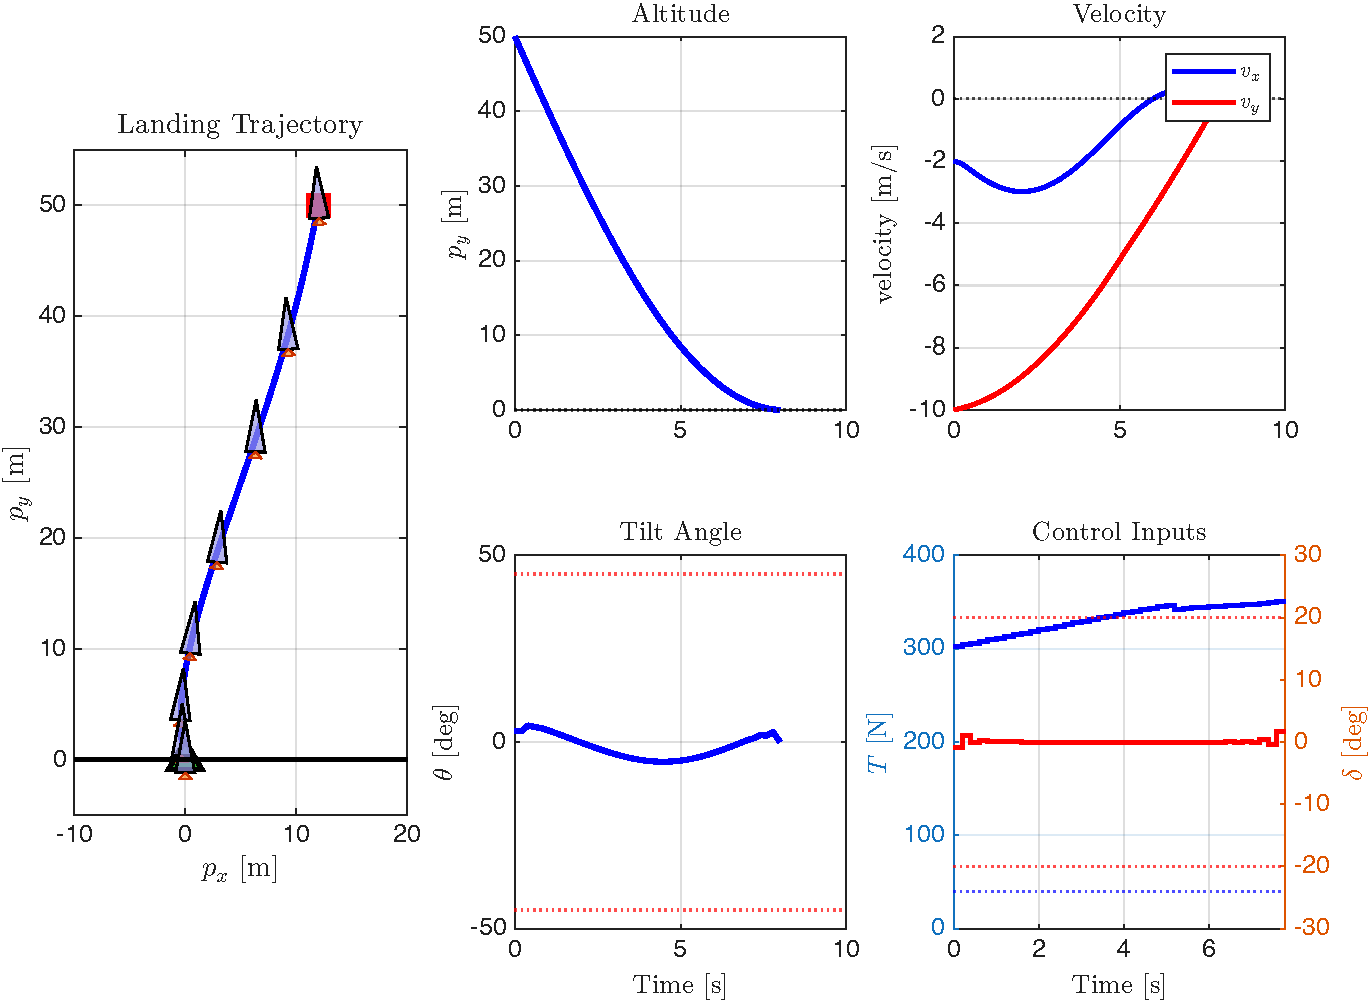
\includegraphics[width=0.9\textwidth]{Figures/fig_nmpc_rocket_traj.pdf}
	\caption{Rocket landing trajectory computed by SCvx. Left: 2D trajectory with rocket attitude at selected time steps. The rocket corrects horizontal drift, decelerates, and lands vertically at the target. Right, top to bottom: altitude, velocity components, tilt angle, and thrust/gimbal inputs. Dashed lines indicate constraint limits.}
	\label{fig:nmpc_rocket_traj}
\end{figure}

\begin{figure}[ht]
	\centering
	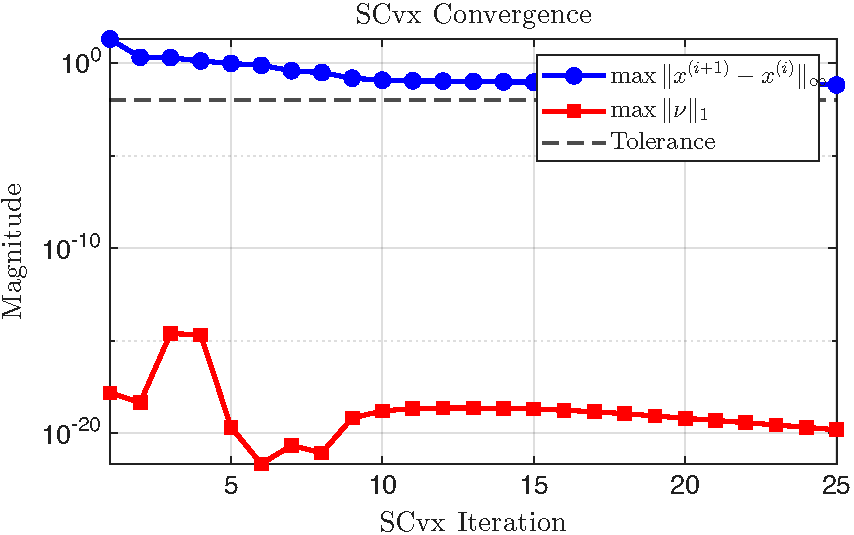
\includegraphics[width=0.7\textwidth]{Figures/fig_scvx_convergence.pdf}
	\caption{SCvx convergence: maximum trajectory change $\max_k\|x_k^{(i+1)} - x_k^{(i)}\|_\infty$ and virtual control magnitude $\max_k\|\nu_k\|_1$ versus iteration. Both quantities decrease below the tolerance $10^{-3}$ within approximately 10 iterations.}
	\label{fig:scvx_convergence}
\end{figure}


% ================================================================
% REAL-TIME NMPC
% ================================================================
\section{Real-Time Nonlinear MPC}
\label{sec:rt_nmpc}

In a receding-horizon loop, the NLP (or SCP sequence) must be solved within one sampling period $T_s$. For fast systems ($T_s$ in the millisecond range), this is the primary bottleneck.

\subsection{The Real-Time Iteration (RTI)}
\label{sec:rti}

The \emph{Real-Time Iteration} scheme~\cite{Diehl2005} exploits the fact that consecutive MPC problems differ only slightly (the state has moved by one step). Instead of solving each NLP to convergence, RTI performs a \emph{single SQP iteration} per sampling instant:

\begin{enumerate}[nosep]
	\item \textbf{Preparation phase} (between samples): linearise the dynamics and form the QP using the \emph{shifted} previous solution as the reference trajectory.
	\item \textbf{Feedback phase} (at the sampling instant): update the initial state $x_0 = x(t)$, solve the QP, and apply $u_0^*$.
\end{enumerate}

The feedback phase involves only a QP solve---typically microseconds to milliseconds for structured solvers. Over successive time steps, the single-iteration updates accumulate into full NLP convergence, provided the system evolves continuously. RTI is the workhorse of real-time NMPC and is implemented in the \emph{acados} framework~\cite{Verschueren2022}.

\begin{notebox}{RTI and Successive Linearisation}
	RTI is closely related to the successive linearisation of Section~\ref{sec:tracking_mpc}: both perform one linearisation and one QP solve per time step. The difference is that RTI linearises around the \emph{shifted previous solution} (which tracks the actual trajectory), whereas successive linearisation in Section~\ref{sec:tracking_mpc} uses the \emph{known reference trajectory}. RTI is more general---it does not require a reference.
\end{notebox}

\subsection{Warm-Starting and Shifted Initialisation}

At time $t$, the previous solution provides a trajectory $x_0^*, x_1^*, \dots, x_N^*$ and controls $u_0^*, u_1^*, \dots, u_{N-1}^*$. The \emph{shifted initialisation} for the next time step is:
\[
\bar{x}_k^{\text{new}} = x_{k+1}^*, \;\; k = 0, \dots, N{-}1, \qquad \bar{x}_N^{\text{new}} = f(x_N^*, u_{N-1}^*),
\]
\[
\bar{u}_k^{\text{new}} = u_{k+1}^*, \;\; k = 0, \dots, N{-}2, \qquad \bar{u}_{N-1}^{\text{new}} = u_{N-1}^*.
\]
This provides an excellent initial guess for the NLP solver (or SCvx), dramatically reducing the number of iterations needed.


% ================================================================
% PRACTICAL GUIDELINES
% ================================================================
\section{Practical Guidelines}
\label{sec:nmpc_guidelines}

\begin{summarybox}{Comparison of NMPC Solution Methods}
	\begin{center}
		\renewcommand{\arraystretch}{1.3}
		\begin{tabular}{p{0.16\textwidth} p{0.16\textwidth} p{0.16\textwidth} p{0.16\textwidth} p{0.16\textwidth}}
			\toprule
			& \textbf{Full NLP} & \textbf{SCvx} & \textbf{GuSTO} & \textbf{RTI} \\
			\midrule
			\textbf{Subproblem} & NLP (IPOPT) & QP/SOCP & QP & QP \\
			\textbf{Iterations} & To convergence & 5--15 & 5--15 & 1 per step \\
			\textbf{Tools} & CasADi & YALMIP/CVX & YALMIP/CVX & acados \\
			\textbf{Guarantees} & Local NLP & KKT point & KKT point & Asymptotic \\
			\textbf{Computation} & ms--s & $<$ ms each & $<$ ms each & $\mu$s--ms \\
			\textbf{Best for} & Offline / slow & Trajectory opt. & Trajectory opt. & Real-time \\
			\bottomrule
		\end{tabular}
	\end{center}
\end{summarybox}

\textbf{When to use what:}
\begin{itemize}[nosep]
	\item \textbf{Small system, slow dynamics} ($T_s > 100$\,ms): Full NLP via CasADi/IPOPT is the simplest and most flexible.
	\item \textbf{Trajectory optimisation} (offline planning): SCvx or GuSTO. The QP subproblems are fast and the convergence is reliable.
	\item \textbf{Fast dynamics} ($T_s < 10$\,ms): RTI with acados. One QP per step, microsecond feedback.
	\item \textbf{Safety-critical}: SCvx or GuSTO with convergence verification. The convex subproblems have certified solvers and no risk of converging to a poor local minimum of the subproblem.
\end{itemize}


% ================================================================
% SUMMARY
% ================================================================
\section*{Summary}

\begin{summarybox}{Nonlinear MPC}
	\begin{enumerate}[nosep]
		\item NMPC replaces linear dynamics $Ax + Bu$ with the full nonlinear model $f(x, u)$. The resulting optimisation is a non-convex NLP.
		\item \textbf{Direct multiple shooting} is the standard transcription: both states and controls are decision variables, dynamics are equality constraints, and the NLP has exploitable sparsity.
		\item \textbf{CasADi + IPOPT} provides a complete NLP workflow with automatic differentiation. Suitable for offline or slow real-time applications.
		\item \textbf{Sequential convex programming} (SCvx, GuSTO) replaces the NLP with a sequence of QPs by linearising the dynamics at each iteration. Trust regions or penalty terms ensure convergence.
		\item \textbf{Real-Time Iteration} performs one SQP/QP step per sampling instant, enabling NMPC at millisecond rates.
		\item The choice of method depends on the sampling rate, system size, and certification requirements.
	\end{enumerate}
\end{summarybox}


% ================================================================
% EXERCISES
% ================================================================
\section*{Exercises}
\begin{enumerate}

\item \textbf{(Direct Multiple Shooting for a Van der Pol Oscillator)}
Consider the Van der Pol oscillator:
\[
\dot{x}_1 = x_2, \qquad \dot{x}_2 = \mu(1 - x_1^2)\,x_2 - x_1 + u,
\]
with $\mu = 1$, $|u| \le 1$, $T_s = 0.1$\,s, $N = 20$.
\begin{enumerate}
	\item Discretise using Forward Euler. Write out the nonlinear discrete-time equations.
	\item Formulate the direct multiple shooting NLP for driving $x_0 = [2;\; 0]$ to the origin with cost $\sum x_k^\top I\, x_k + 0.1\, u_k^2$. State all decision variables and constraints.
	\item Implement in MATLAB using \texttt{fmincon}. Plot the resulting state and control trajectories. Does the solver converge from a zero initial guess?
	\item Compare the solution obtained from two different initial guesses. Does the NLP have multiple local minima?
\end{enumerate}

\item \textbf{(SCvx for Nonlinear Path Planning)}
A point mass in 2D with state $x = [p_x,\; p_y,\; v_x,\; v_y]^\top$ and input $u = [a_x,\; a_y]^\top$ has linear dynamics $\dot{p} = v$, $\dot{v} = u$, with $\|u\|_2 \le a_{\max}$. An obstacle at position $p_{\text{obs}}$ with radius $r_{\text{obs}}$ imposes the non-convex constraint $\|p_k - p_{\text{obs}}\|_2 \ge r_{\text{obs}}$.
\begin{enumerate}
	\item Show that the obstacle avoidance constraint is non-convex.
	\item Linearise the obstacle constraint at a point $\bar{p}_k$ to obtain a halfspace approximation. Write out the resulting linear inequality.
	\item Implement SCvx in MATLAB/YALMIP with $a_{\max} = 2$, $p_{\text{obs}} = [5;\; 0]$, $r_{\text{obs}} = 2$, initial state $(0, 0, 1, 0)$, target $(10, 0, 0, 0)$, $N = 40$, $T_s = 0.2$\,s. Plot the trajectory at iterations 1, 3, 5, and convergence.
	\item What happens if the initial trajectory guess passes through the obstacle? Does SCvx still converge?
\end{enumerate}

\item \textbf{(Rocket Landing: Sensitivity Analysis)}
Using the rocket model from Section~\ref{sec:rocket_landing} with the parameters given:
\begin{enumerate}
	\item Modify the initial horizontal offset to $p_{x,0} = 0$ (directly above the target). How does the optimal trajectory change? Does the rocket still need to tilt?
	\item Increase the minimum thrust to $T_{\min} = 100$\,N. How does this affect the descent profile? At what $T_{\min}$ does the problem become infeasible?
	\item Replace the fuel-optimal cost ($\min \sum T_k$) with a time-optimal cost. Formulate the modified problem and discuss the challenges of free-final-time optimisation in the SCvx framework.
\end{enumerate}

\item \textbf{(Comparing SCvx and GuSTO)}
Implement both SCvx (with trust region $\Delta = 50$) and GuSTO (with initial penalty $\lambda = 0.1$) for the rocket landing problem.
\begin{enumerate}
	\item Plot the number of iterations to convergence for each method as a function of the initial trajectory guess quality (vary the initial guess from ``poor'' --- constant hover thrust --- to ``good'' --- a preliminary trajectory from a coarser discretisation).
	\item Compare the final cost (total fuel) achieved by each method. Are they the same?
	\item Which method is more sensitive to the initial guess?
\end{enumerate}

\item \textbf{(Real-Time Iteration for a Nonlinear System)}
Consider the pendulum from Section~\ref{sec:nmpc_nlp} in a receding-horizon loop.
\begin{enumerate}
	\item Implement the full NMPC controller (solving the NLP to convergence at each step using \texttt{fmincon} or CasADi). Record the computation time per step.
	\item Implement RTI: at each step, perform a single SCvx iteration using the shifted previous solution. Record the computation time.
	\item Compare the closed-loop trajectories. For what initial conditions do the two approaches produce different results? Discuss the trade-off between computation time and optimality.
\end{enumerate}

\item \textbf{(Lossless Convexification)}
Consider a point-mass rocket in 2D with state $x = [p_x,\; p_y,\; v_x,\; v_y]^\top$ and thrust vector $T = [T_x,\; T_y]^\top$ (the input is the 2D thrust directly, not magnitude/angle). The constraint is $T_{\min} \le \|T\| \le T_{\max}$.
\begin{enumerate}
	\item Show that the constraint $T_{\min} \le \|T\|$ is non-convex by sketching the feasible set in $(T_x, T_y)$ space.
	\item The \emph{lossless convexification} relaxation introduces a slack variable $\Gamma$ and replaces the constraint with: $\|T\| \le \Gamma$, $T_{\min} \le \Gamma \le T_{\max}$. Show that this feasible set is convex.
	\item Argue (intuitively or formally) that at the optimum of a fuel-minimisation problem ($\min \sum \Gamma_k$), the relaxation is \emph{tight}: $\|T^*_k\| = \Gamma^*_k$. Why would the optimiser never waste fuel by having $\|T_k\| < \Gamma_k$?
\end{enumerate}

\end{enumerate}

	\chapter{MPC with Learning\texorpdfstring{$^{(*)}$}{(*)}}
\label{chap:learning_mpc}

\begin{quote}
	\textit{``All models are wrong, but some are useful.''} \\
	\hfill --- \emph{George E.\,P.\ Box} (1976)
\end{quote}

Every MPC controller we have built so far starts from the same assumption: a known, accurate model $x_{k+1} = Ax_k + Bu_k$. Chapters~\ref{chap:lqr}--\ref{chap:output_fb_mpc} derive the optimal control law, the estimator, and the constraint-handling machinery on top of this model. Tube MPC relaxes the assumption slightly, admitting bounded disturbances, but still requires the system matrices $A$ and $B$ and a known disturbance bound $\mathcal{W}$.

In many practical situations, however, the model is the bottleneck. Three distinct problems arise:
\begin{enumerate}
	\item \emph{Model inaccuracy.} The identified $A$ and $B$ are approximate. The true dynamics contain terms the model ignores---friction, aerodynamic drag, thermal coupling.
	\item \emph{Model incompleteness.} Part of the dynamics is entirely unknown. A robot grasping an unfamiliar object does not know the object's mass or friction coefficient.
	\item \emph{No model at all.} For some systems---biological processes, soft robots, complex chemical reactors---first-principles modelling is prohibitively difficult. Only input--output data is available.
\end{enumerate}

This chapter introduces methods that combine \emph{learning from data} with \emph{MPC}. The central question is: \emph{how can we use measured data to replace, correct, or bypass the model, while retaining the constraint-handling and optimality guarantees that make MPC attractive?}

\section{Three Paradigms for Learning in MPC}
\label{sec:learning_paradigms}

The methods in this chapter fall into three families, distinguished by \emph{what} is learned.

\begin{defnbox}{Three Paradigms}
	\begin{enumerate}
		\item \emph{Model Learning.} Learn the unknown dynamics $f(x,u)$---or a correction to a nominal model---from data. Then use the learned model inside a standard MPC formulation.\\
		\emph{Methods:} Gaussian Process MPC (Section~\ref{sec:gpmpc}), Neural Network MPC (Section~\ref{sec:nnmpc}).

		\item \emph{Data-Driven Control.} Use trajectory data to construct a linear prediction model or bypass system identification entirely.\\
		\emph{Methods:} Koopman/EDMD MPC (Section~\ref{sec:koopman}), DeePC (Section~\ref{sec:deepc}).\\
		\emph{Note:} Koopman/EDMD identifies matrices $(A_K, B_K)$ from data---an indirect data-driven approach. DeePC uses data directly without ever forming an explicit model.

		\item \emph{Policy Learning.} Use closed-loop experience from previous task executions to improve the MPC policy itself---expanding the safe region and reducing cost over repeated attempts.\\
		\emph{Methods:} Learning MPC (Section~\ref{sec:lmpc}).
	\end{enumerate}
\end{defnbox}

\begin{notebox}{Connection to Earlier Chapters}
	Each approach builds on tools already developed in these notes:
	\begin{center}
		\begin{tabular}{l l}
			\toprule
			\emph{Approach} & \emph{Prerequisites} \\
			\midrule
			GP-MPC & Ch.\,6 (Bayesian estimation), Ch.\,7 (constrained MPC), Tube MPC (uncertainty) \\
			Koopman MPC & Ch.\,3 (state-space), Ch.\,5 (QP/LQR), Ch.\,7 (linear MPC) \\
			DeePC & Ch.\,2 (optimisation/YALMIP), Ch.\,7 (MPC formulation) \\
			LMPC & Ch.\,7 (terminal sets, recursive feasibility) \\
			\bottomrule
		\end{tabular}
	\end{center}
\end{notebox}

\begin{alertbox}{When is learning necessary?}
	Not every MPC application needs learning. If a first-principles model is available and accurate, standard MPC (Chapter~7) or Tube MPC are preferable---they are simpler to implement and their guarantees are better understood. Learning is most valuable when:
	\begin{itemize}[noitemsep]
		\item The model is too expensive or too difficult to derive from physics.
		\item The system changes over time (wear, ageing, varying loads).
		\item The disturbance structure is unknown or state-dependent, so that fixed bounds $\mathcal{W}$ are overly conservative.
	\end{itemize}
\end{alertbox}

Figure~\ref{fig:learning_taxonomy} summarises the three paradigms and the methods covered in this chapter.

\begin{figure}[ht]
	\centering
	\resizebox{\linewidth}{!}{%
	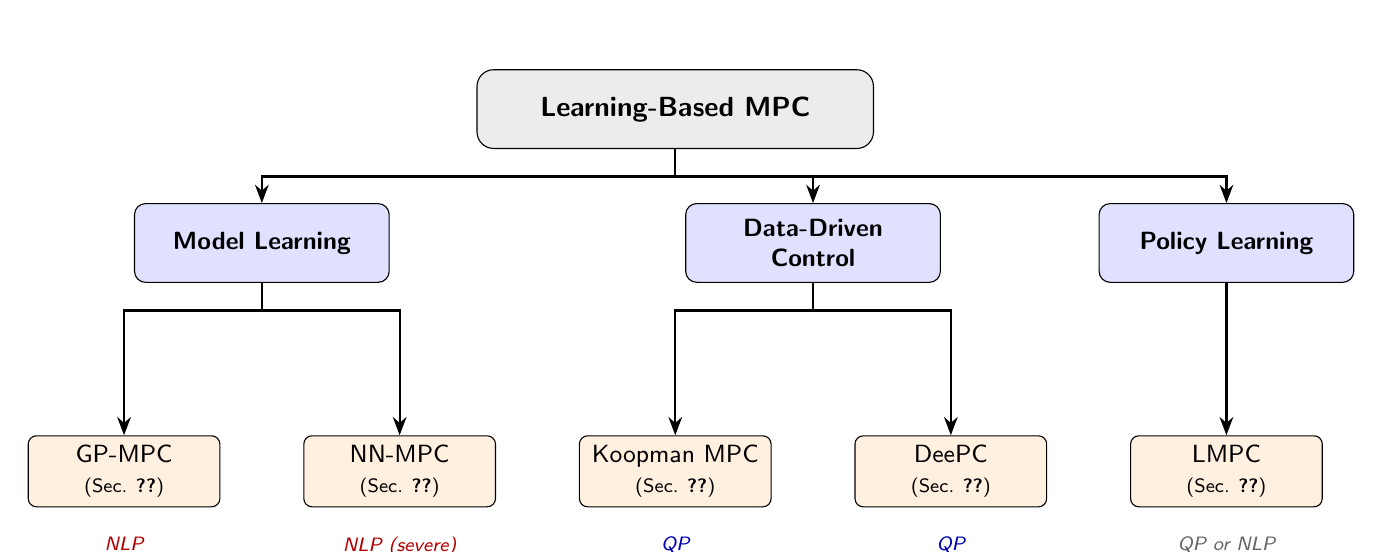
\begin{tikzpicture}[
		>=Stealth,
		paradigm/.style={draw, rounded corners=4pt, fill=blue!12,
			text width=3.0cm, minimum height=1.0cm, align=center,
			font=\small\bfseries},
		method/.style={draw, rounded corners=3pt, fill=orange!12,
			text width=2.2cm, minimum height=0.8cm, align=center,
			font=\small},
		root/.style={draw, rounded corners=6pt, fill=gray!15,
			text width=4.8cm, minimum height=1.0cm, align=center,
			font=\normalsize\bfseries},
	]
		% Root
		\node[root] at (0,0) (root) {Learning-Based MPC};

		% Paradigms — centres above their child groups
		\node[paradigm] at (-5.25,-1.7) (p1) {Model Learning};
		\node[paradigm] at (1.75,-1.7)  (p2) {Data-Driven\\Control};
		\node[paradigm] at (7.0,-1.7)   (p3) {Policy Learning};

		% Arrows from root to paradigms
		\draw[->, thick] (root.south) -- ++(0,-0.35) -| (p1.north);
		\draw[->, thick] (root.south) -- ++(0,-0.35) -| (p2.north);
		\draw[->, thick] (root.south) -- ++(0,-0.35) -| (p3.north);

		% Methods — 5 leaf nodes with 3.5cm centre-to-centre spacing (≈1cm gap)
		\node[method] at (-7.0,-4.6) (m1a) {GP-MPC\\{\scriptsize (Sec.~\ref{sec:gpmpc})}};
		\node[method] at (-3.5,-4.6) (m1b) {NN-MPC\\{\scriptsize (Sec.~\ref{sec:nnmpc})}};
		\node[method] at (0.0,-4.6)  (m2a) {Koopman MPC\\{\scriptsize (Sec.~\ref{sec:koopman})}};
		\node[method] at (3.5,-4.6)  (m2b) {DeePC\\{\scriptsize (Sec.~\ref{sec:deepc})}};
		\node[method] at (7.0,-4.6)  (m3a) {LMPC\\{\scriptsize (Sec.~\ref{sec:lmpc})}};

		% Arrows from paradigms to methods
		\draw[->, thick] (p1.south) -- ++(0,-0.35) -| (m1a.north);
		\draw[->, thick] (p1.south) -- ++(0,-0.35) -| (m1b.north);
		\draw[->, thick] (p2.south) -- ++(0,-0.35) -| (m2a.north);
		\draw[->, thick] (p2.south) -- ++(0,-0.35) -| (m2b.north);
		\draw[->, thick] (p3.south) -- (m3a.north);

		% Annotations: QP vs NLP
		\node[below=0.25cm of m1a, font=\scriptsize\itshape, text=red!70!black] {NLP};
		\node[below=0.25cm of m1b, font=\scriptsize\itshape, text=red!70!black] {NLP (severe)};
		\node[below=0.25cm of m2a, font=\scriptsize\itshape, text=blue!70!black] {QP};
		\node[below=0.25cm of m2b, font=\scriptsize\itshape, text=blue!70!black] {QP};
		\node[below=0.25cm of m3a, font=\scriptsize\itshape, text=black!60] {QP or NLP};
	\end{tikzpicture}%
	}
	\caption{Taxonomy of learning-based MPC methods. Model learning approaches (GP-MPC, NN-MPC) learn the unknown dynamics and embed the learned model in MPC. Data-driven approaches (Koopman MPC, DeePC) use data directly, preserving the QP structure of linear MPC. Policy learning (LMPC) improves the controller from repeated task executions. The annotation below each method indicates whether the resulting online optimisation is a convex QP or a non-convex NLP.}
	\label{fig:learning_taxonomy}
\end{figure}


%% ============================================================
%%  SECTION 2: GAUSSIAN PROCESS MPC
%% ============================================================
\section{Gaussian Process MPC}
\label{sec:gpmpc}

Suppose we have a nominal model $x_{k+1} = Ax_k + Bu_k$ that captures the dominant dynamics, but the true system contains an additional unknown term:
\begin{equation}\label{eq:residual_model}
	x_{k+1} = Ax_k + Bu_k + g(x_k, u_k)
\end{equation}
where $g \colon \mathbb{R}^n \times \mathbb{R}^m \to \mathbb{R}^n$ is an unknown function representing unmodelled dynamics. The idea behind GP-MPC is to learn $g$ from data as a \emph{Gaussian process}---a probabilistic model that provides not only a best-guess prediction but also a measure of confidence. This confidence is then used to tighten the MPC constraints adaptively: more in regions where data is sparse and the model is uncertain, less where data is dense and the model is reliable.

\subsection{Gaussian Process Regression}
\label{sec:gp_regression}

A Gaussian process is a tool for learning an unknown function from noisy observations. The reader needs basic probability from Appendix~B; in particular, the conditional multivariate Gaussian (Section~\ref{sec:app_cond_gauss}) is the mathematical foundation of GP prediction, and the chance-constraint conversion (Section~\ref{sec:app_chance_constraints}) is used for constraint tightening in Section~\ref{sec:gpmpc_formulation}.

\subsubsection*{The Setup}

We have $T$ noisy observations of an unknown scalar function $f$:
\[
y_i = f(x_i) + \varepsilon_i, \qquad \varepsilon_i \sim \mathcal{N}(0, \sigma_n^2), \qquad i = 1, \ldots, T
\]
where $x_i$ is the input (which may be a vector), $y_i$ is the observed output, and $\varepsilon_i$ is independent Gaussian noise with variance $\sigma_n^2$. Given these $T$ pairs, we want to predict $f(x_*)$ at a new test point $x_*$.

\subsubsection*{The Gaussian Process Prior}

A parametric model (e.g.\ a polynomial) commits to a fixed functional form and learns its coefficients. A Gaussian process takes a different approach: it places a probability distribution directly over \emph{functions}.

\begin{defnbox}{Definition: Gaussian Process}
	A \emph{Gaussian process} (GP) is a collection of random variables, any finite subset of which has a joint Gaussian distribution. A GP is fully specified by its \emph{mean function} $m(x)$ and \emph{covariance function} (or \emph{kernel}) $k(x, x')$:
	\[
	f \sim \mathcal{GP}\bigl(m(x),\; k(x, x')\bigr)
	\]
	For any finite set of inputs $\{x_1, \ldots, x_T\}$, the function values $[f(x_1), \ldots, f(x_T)]^\top$ are jointly Gaussian with mean $[m(x_1), \ldots, m(x_T)]^\top$ and covariance matrix $K_{ij} = k(x_i, x_j)$.
\end{defnbox}

We typically set $m(x) = 0$ (the prior mean is zero, meaning no prior bias), so that all structure in the function is captured by the kernel $k(x, x')$.

\subsubsection*{The Kernel}

The kernel encodes our assumptions about the unknown function: how smooth it is, how fast it varies, and over what length scales. The most common choice is the \emph{squared exponential} (SE) kernel:
\begin{equation}\label{eq:se_kernel}
	k(x, x') = \sigma_f^2 \exp\!\left(-\frac{\|x - x'\|^2}{2\ell^2}\right)
\end{equation}
This kernel has two hyperparameters:
\begin{itemize}[noitemsep]
	\item $\sigma_f^2$ (\emph{signal variance}): controls the overall amplitude of the function. Larger $\sigma_f$ allows the function to take larger values.
	\item $\ell$ (\emph{length scale}): controls how quickly the function can change. A small $\ell$ permits rapid variation; a large $\ell$ enforces smooth, slowly varying behaviour.
\end{itemize}
When two inputs $x$ and $x'$ are close ($\|x - x'\| \ll \ell$), the kernel is close to $\sigma_f^2$, meaning the function values are highly correlated. When they are far apart ($\|x - x'\| \gg \ell$), the kernel approaches zero and the function values are nearly independent.

\subsubsection*{The Prediction Equations}

Given training inputs $\{x_1, \ldots, x_T\}$, observations $y = [y_1, \ldots, y_T]^\top$, and a test point $x_*$, the GP posterior is Gaussian with:
\begin{align}
	\mu_*(x_*) &= k_*^\top \bigl(K + \sigma_n^2 I\bigr)^{-1} y \label{eq:gp_mean} \\[4pt]
	\sigma_*^2(x_*) &= k(x_*, x_*) - k_*^\top \bigl(K + \sigma_n^2 I\bigr)^{-1} k_* \label{eq:gp_var}
\end{align}
where:
\begin{itemize}[noitemsep]
	\item $K \in \mathbb{R}^{T \times T}$ is the \emph{Gram matrix} with entries $K_{ij} = k(x_i, x_j)$.
	\item $k_* = [k(x_*, x_1), \ldots, k(x_*, x_T)]^\top \in \mathbb{R}^T$ is the vector of kernel evaluations between the test point and all training points.
	\item $\sigma_n^2$ is the noise variance.
\end{itemize}

\begin{summarybox}{GP Prediction Recipe}
	Given training data $\{(x_i, y_i)\}_{i=1}^T$ and a test input $x_*$:
	\begin{enumerate}[noitemsep]
		\item Build the Gram matrix $K$ and the test kernel vector $k_*$.
		\item Compute $\alpha = (K + \sigma_n^2 I)^{-1}y$ (solve a linear system---do not invert the matrix explicitly).
		\item The \emph{predicted mean} is $\mu_* = k_*^\top \alpha$.
		\item The \emph{predicted variance} is $\sigma_*^2 = k(x_*,x_*) - k_*^\top (K + \sigma_n^2 I)^{-1}k_*$.
	\end{enumerate}
	The mean $\mu_*$ is the best prediction. The interval $\mu_* \pm 2\sigma_*$ is a 95\% confidence band.
\end{summarybox}

\begin{examplebox}{GP Regression on a Scalar Function}
	We observe 10 noisy samples from $f(x) = \sin(x)$ on the interval $[0, 2\pi]$:
	\[
	y_i = \sin(x_i) + \varepsilon_i, \qquad \varepsilon_i \sim \mathcal{N}(0, 0.04), \qquad i = 1, \ldots, 10
	\]
	We use the SE kernel~\eqref{eq:se_kernel} with $\sigma_f = 1$, $\ell = 1$, and $\sigma_n = 0.2$.

	\solution

	For a test point $x_* = 1.5$:
	\begin{enumerate}
		\item Compute the $10 \times 10$ Gram matrix $K$ using $k(x_i, x_j) = \exp\bigl(-\frac{(x_i - x_j)^2}{2}\bigr)$.
		\item Compute $k_* \in \mathbb{R}^{10}$, where each entry is $k(1.5, x_i)$.
		\item Solve the linear system $(K + 0.04\,I)\,\alpha = y$.
		\item The predicted mean is $\mu_* = k_*^\top \alpha$.
		\item The predicted variance is $\sigma_*^2 = 1 - k_*^\top (K + 0.04\,I)^{-1}k_*$.
	\end{enumerate}

	The resulting mean $\mu_*$ will be close to $\sin(1.5) \approx 0.997$, and the variance $\sigma_*^2$ will be small because $x_* = 1.5$ is close to several training points. In regions far from any training data, the variance grows, reflecting genuine uncertainty.

The following MATLAB script implements this example.

\begin{lstlisting}[language=Matlab, caption={GP regression for $f(x)=\sin(x)$ from noisy data.}]
% 1. Training Data
rng(42);
T  = 10;
X  = sort(2*pi*rand(T,1));
sn = 0.2;
y  = sin(X) + sn*randn(T,1);

% 2. Kernel Hyperparameters
sf = 1;  ell = 1;  sn2 = sn^2;

% 3. Kernel Function
kSE = @(xa,xb) sf^2*exp(-0.5*(xa-xb').^2/ell^2);

% 4. Gram Matrix and Alpha
K     = kSE(X, X);
alpha = (K + sn2*eye(T)) \ y;

% 5. Predictions on a Dense Grid
Xstar  = linspace(0, 2*pi, 200)';
Kstar  = kSE(Xstar, X);
Kss    = kSE(Xstar, Xstar);
mu     = Kstar * alpha;
V      = Kss - Kstar * ((K + sn2*eye(T)) \ Kstar');
sig    = sqrt(diag(V));

% 6. Plot
figure; hold on;
fill([Xstar; flipud(Xstar)], ...
     [mu+2*sig; flipud(mu-2*sig)], ...
     [0.8 0.9 1], 'EdgeColor','none');
plot(Xstar, mu, 'b-', 'LineWidth', 2);
plot(X, y, 'ko', 'MarkerFaceColor','k', 'MarkerSize', 6);
plot(Xstar, sin(Xstar), 'r--', 'LineWidth', 1.5);
xlabel('x'); ylabel('f(x)');
legend('95\% confidence', 'GP mean', 'Data', 'True f(x)');
title('GP Regression'); hold off;
\end{lstlisting}
\end{examplebox}

The result of this code is shown in Figure~\ref{fig:gp_regression}. The GP mean (blue) closely tracks the true function $\sin(x)$ (red dashed) near the training points, while the $\pm 2\sigma$ confidence band (shaded blue) widens in regions where data is sparse---precisely where prediction uncertainty is greatest.

\begin{figure}[ht]
	\centering
	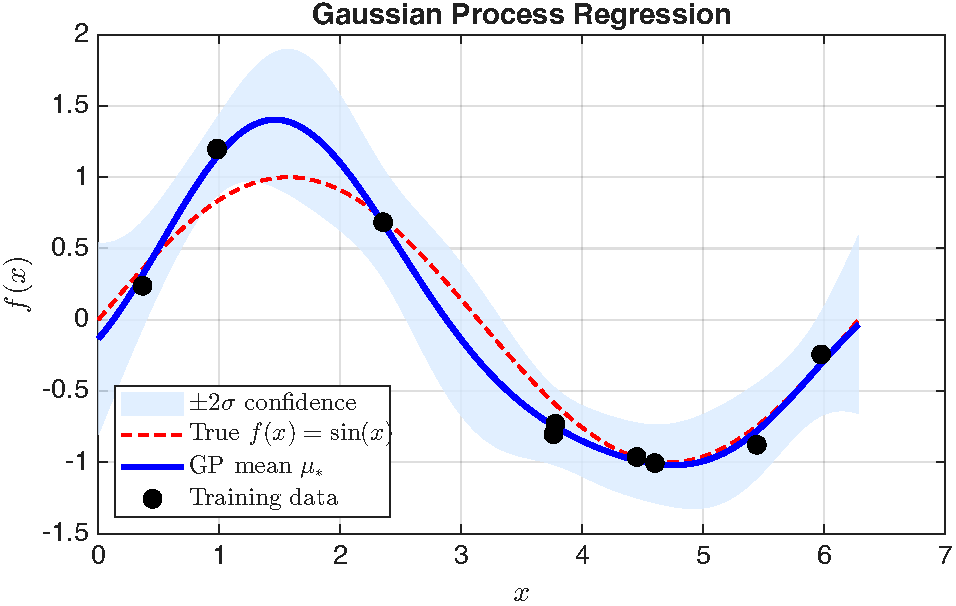
\includegraphics[width=0.85\textwidth]{Figures/fig_gp_regression.pdf}
	\caption{Gaussian Process regression on noisy observations of $f(x) = \sin(x)$. The GP mean interpolates the training data, and the 95\% confidence band widens away from data points, reflecting increasing prediction uncertainty. With 10 observations and a squared exponential kernel ($\sigma_f = 1$, $\ell = 1$), the GP captures the sinusoidal shape while honestly reporting its confidence.}
	\label{fig:gp_regression}
\end{figure}


\subsection{Learning Unknown Dynamics with GPs}
\label{sec:gp_dynamics}

Returning to the residual model~\eqref{eq:residual_model}, suppose we have collected $T$ state transitions from the real plant:
\[
\{(x_k, u_k, x_{k+1})\}_{k=0}^{T-1}
\]
The residual at each time step is:
\begin{equation}\label{eq:residual_data}
	r_k = x_{k+1} - Ax_k - Bu_k
\end{equation}
This is the part of the dynamics the nominal model fails to explain. Each $r_k$ is a noisy observation of $g(x_k, u_k)$.

For a system with $n$ states, $g$ maps $\mathbb{R}^{n+m}$ to $\mathbb{R}^n$. We fit \emph{one independent GP per state dimension}: the $i$th GP is trained on inputs $\{(x_k, u_k)\}$ and outputs $\{r_{k,i}\}$, where $r_{k,i}$ is the $i$th component of $r_k$.

After training, given a current state $x$ and input $u$, the GP provides:
\begin{align*}
	\text{Predicted next state:} \quad & \hat{x}_{k+1} = Ax_k + Bu_k + \mu_g(x_k, u_k) \\
	\text{Prediction uncertainty:} \quad & \Sigma_{k+1} = \text{diag}\bigl(\sigma_{g,1}^2(x_k, u_k), \ldots, \sigma_{g,n}^2(x_k, u_k)\bigr)
\end{align*}
where $\mu_g$ and $\Sigma_{k+1}$ are assembled from the individual GP predictions.

\begin{alertbox}{Computational Complexity}
	GP prediction requires solving a $T \times T$ linear system, which scales as $O(T^3)$. For small to moderate datasets ($T < 500$), this is fast. For larger datasets, sparse GP approximations using \emph{inducing points} reduce the cost to $O(TM^2)$, where $M \ll T$ is the number of inducing points. For the examples in these notes, exact GP inference is sufficient.
\end{alertbox}

Figure~\ref{fig:gp_residual} illustrates this process for the worked example in Section~\ref{sec:gpmpc_example}: the GP learns the unknown cubic drag $g(x) = -0.2\,x^3$ from 20 residual data points. The confidence band is narrow where data is concentrated and widens at the extremes.

\begin{figure}[ht]
	\centering
	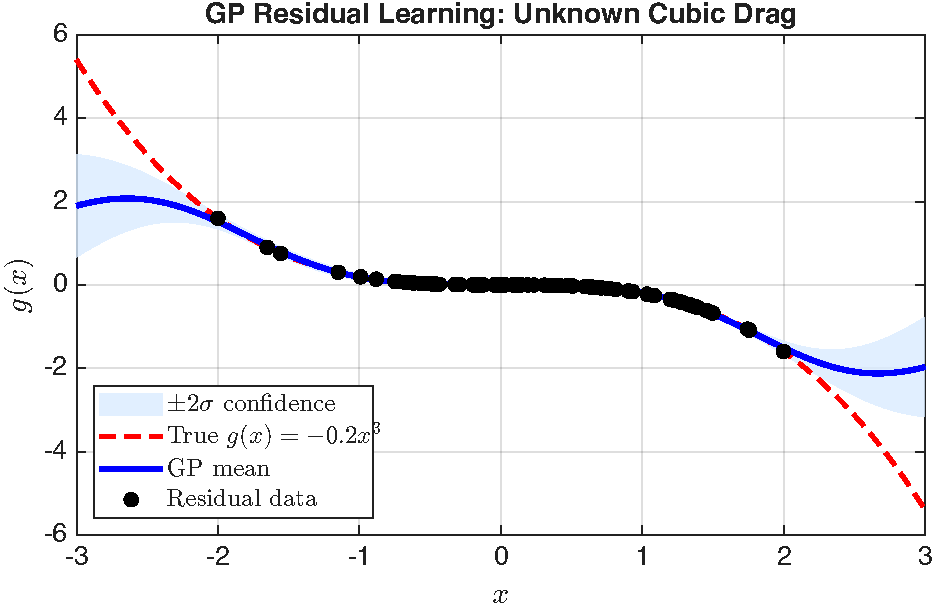
\includegraphics[width=0.85\textwidth]{Figures/fig_gp_residual.pdf}
	\caption{GP residual learning for the unknown cubic drag $g(x) = -0.2\,x^3$. The GP mean (blue) closely matches the true residual (red dashed) in the data-rich region $|x| \lesssim 2$, while the 95\% confidence band (shaded) widens outside this range. The black dots are the computed residuals $r_k = x_{k+1} - x_k - u_k$ from 20 exploratory data points.}
	\label{fig:gp_residual}
\end{figure}


\subsection{The GP-MPC Optimisation Problem}
\label{sec:gpmpc_formulation}

At each time step, the GP-enhanced model predicts the mean trajectory and the state-dependent uncertainty. This uncertainty is exploited through \emph{chance constraints}: instead of requiring that constraints hold with certainty (which would require worst-case reasoning as in Tube MPC), we require that they hold with a specified probability $1 - \delta$.

For each state dimension $i$ and each prediction step $k$, the state constraint $x_{k,i} \le x_{\max,i}$ becomes:
\begin{equation}\label{eq:chance_constraint}
	\Pr\bigl(x_{k,i} \le x_{\max,i}\bigr) \ge 1 - \delta
\end{equation}
For a \emph{single} prediction step, if the GP prediction is Gaussian, this is equivalent to a deterministic tightened constraint:
\begin{equation}\label{eq:tightened_chance}
	\boxed{\mu_{k,i} + \Phi^{-1}(1-\delta)\;\sigma_{k,i} \le x_{\max,i}}
\end{equation}
where $\Phi^{-1}$ is the inverse of the standard normal CDF (e.g.\ $\Phi^{-1}(0.95) \approx 1.645$ for a 95\% constraint, $\Phi^{-1}(0.975) \approx 1.96$ for 97.5\%).

\begin{alertbox}{Multi-Step Validity}
	The Gaussian tightening~\eqref{eq:tightened_chance} is exact at the first prediction step ($k=1$), because the one-step GP prediction is Gaussian by construction. For $k > 1$, the predicted state distribution is obtained by propagating through the nonlinear GP mean, which destroys the Gaussian structure. In practice, the formula is applied at every horizon step as a tractable \emph{approximation}---evaluating the GP variance at the current nominal trajectory rather than propagating uncertainty forward. This ``certainty-equivalent'' approach works well when the GP variance is small, but does not provide formal multi-step chance constraint guarantees.
\end{alertbox}

\begin{defnbox}{Chance Constraint Tightening via GP Variance}
	The GP variance $\sigma_{k,i}^2$ acts as a \emph{state-dependent safety margin}. In regions with little training data, $\sigma_{k,i}$ is large, and the constraint is tightened aggressively. In well-explored regions, $\sigma_{k,i}$ is small, and the constraint is barely tightened.
\end{defnbox}

\begin{notebox}{Connection to Tube MPC}
	Tube MPC (previous chapter) tightens constraints by a \emph{fixed} amount $\mathcal{E}$, determined by the worst-case disturbance bound $\mathcal{W}$. GP-MPC tightens constraints \emph{adaptively}: more where data is sparse (high variance), less where data is dense (low variance). As more data is collected, the GP variance shrinks everywhere, and the tightening approaches zero---the controller recovers the full feasible region.
\end{notebox}

The GP-MPC optimisation at time $t$ is:
\begin{equation}\label{eq:gpmpc_opt}
	\min_{u_0, \ldots, u_{N-1}} \; \sum_{k=0}^{N-1}\bigl(\mu_{x_k}^\top Q\,\mu_{x_k} + u_k^\top R\,u_k\bigr) + \mu_{x_N}^\top P\,\mu_{x_N}
\end{equation}
subject to:
\begin{align*}
	\text{Initialisation:} \quad & \mu_{x_0} = x(t) \\
	\text{Learned dynamics:} \quad & \mu_{x_{k+1}} = A\,\mu_{x_k} + B\,u_k + \mu_g(\mu_{x_k}, u_k) \\
	\text{Chance constraints:} \quad & \mu_{x_{k,i}} + \Phi^{-1}(1-\delta)\,\sigma_{x_{k,i}} \le x_{\max,i} \\
	& \mu_{x_{k,i}} - \Phi^{-1}(1-\delta)\,\sigma_{x_{k,i}} \ge x_{\min,i} \\
	\text{Actuator limits:} \quad & u_{\min} \le u_k \le u_{\max}
\end{align*}
for $k = 0, \ldots, N-1$ and $i = 1, \ldots, n$. The terminal cost $P$ is computed from the DARE applied to the nominal $(A, B)$.


\subsection{Worked Example: GP-MPC for a System with Unknown Nonlinearity}
\label{sec:gpmpc_example}

\begin{examplebox}{GP-MPC: Learning an Unknown Cubic Drag}
	\emph{System.} The true plant is a scalar system with a nonlinear drag term:
	\[
	x_{k+1} = x_k + u_k - 0.2\,x_k^3
	\]
	The cubic term $-0.2\,x_k^3$ is unknown to the controller.

	\emph{Nominal model.} The controller uses a pure integrator: $x_{k+1} = x_k + u_k$, i.e.\ $A = 1$, $B = 1$.

	\emph{Constraints.} $|u_k| \le 1$, $|x_k| \le 3$.

	\emph{Objective.} Regulate to the origin from $x_0 = 2.5$ with $Q = 1$, $R = 0.1$, $N = 10$.

	\solution

	\emph{Step 1: Data collection.} We excite the system with 20 random inputs from $u \sim \mathcal{U}(-1, 1)$ starting from $x_0 = 0$, and record the transitions.

	\emph{Step 2: Compute residuals.} For each transition, $r_k = x_{k+1} - x_k - u_k$. These residuals are noisy observations of $g(x_k) = -0.2\,x_k^3$.

	\emph{Step 3: Train GP.} Fit a GP with SE kernel to the residual data. The GP learns $g(x)$ along with pointwise confidence.

	\emph{Step 4: GP-MPC loop.} At each step:
	\begin{enumerate}[noitemsep]
		\item Query the GP at the current predicted states to obtain $\mu_g$ and $\sigma_g$.
		\item Formulate the MPC with tightened constraints: $\mu_{x_k} + 1.96\,\sigma_{x_k} \le 3$ and $\mu_{x_k} - 1.96\,\sigma_{x_k} \ge -3$.
		\item Solve the resulting NLP---or, more commonly, the QP approximation obtained by evaluating the GP at the current nominal trajectory (successive linearisation). Apply $u_0^*$, measure $x_{k+1}$, and optionally append the new data point to the GP training set.
	\end{enumerate}

\begin{lstlisting}[language=Matlab, caption={GP-MPC for a scalar system with unknown cubic drag.}]
% 1. True Plant and Nominal Model
A_nom = 1;  B_nom = 1;
f_true = @(x, u) x + u - 0.2*x^3;

% 2. Data Collection (random excitation)
rng(0);
T_data = 20;
x_data = zeros(T_data+1, 1);
u_data = 2*rand(T_data, 1) - 1;
for k = 1:T_data
    x_data(k+1) = f_true(x_data(k), u_data(k));
end
X_train = x_data(1:T_data);
r_train = x_data(2:T_data+1) - A_nom*x_data(1:T_data) ...
          - B_nom*u_data;

% 3. GP Training (SE kernel)
sf = 0.5;  ell = 1.0;  sn2 = 0.01;
kSE  = @(xa, xb) sf^2*exp(-0.5*(xa - xb').^2 / ell^2);
K_gp = kSE(X_train, X_train) + sn2*eye(T_data);
alpha_gp = K_gp \ r_train;

gp_mean = @(xs) kSE(xs, X_train) * alpha_gp;
gp_var  = @(xs) sf^2 - diag(kSE(xs, X_train) ...
                * (K_gp \ kSE(X_train, xs)));

% 4. GP-MPC Simulation
N = 10;  Q = 1;  R = 0.1;  P = dare(A_nom, B_nom, Q, R);
x_max = 3;  u_max = 1;  delta = 0.025;
kappa = norminv(1 - delta);  % 1.96 for 97.5%

T_sim  = 30;
x_hist = zeros(1, T_sim+1);  x_hist(1) = 2.5;
u_hist = zeros(1, T_sim);

for t = 1:T_sim
    x_now = x_hist(t);
    % Successive linearisation: evaluate GP at nominal trajectory
    x_nom = zeros(1, N+1);  x_nom(1) = x_now;
    mu_nom = zeros(1, N);  sig_nom = zeros(1, N);
    for k = 1:N
        mu_nom(k)  = gp_mean(x_nom(k));
        sig_nom(k) = sqrt(max(gp_var(x_nom(k)), 1e-6));
        x_nom(k+1) = A_nom*x_nom(k) + B_nom*0 + mu_nom(k);  % u=0 nominal
        % Simplification: a production implementation would use the previous MPC solution
    end
    % Build QP with GP evaluated at nominal (fixed, not decision vars)
    u_var = sdpvar(1, N);
    x_var = sdpvar(1, N+1);
    con = [x_var(1) == x_now];
    obj = 0;
    for k = 1:N
        con = [con, x_var(k+1) == A_nom*x_var(k) + B_nom*u_var(k) + mu_nom(k)];
        con = [con, -u_max <= u_var(k) <= u_max];
        con = [con, -x_max + kappa*sig_nom(k) <= x_var(k+1) <= x_max - kappa*sig_nom(k)];
        obj = obj + Q*x_var(k)^2 + R*u_var(k)^2;
    end
    obj = obj + P*x_var(N+1)^2;
    opts = sdpsettings('verbose', 0, 'solver', 'quadprog');
    optimize(con, obj, opts);
    u_hist(t)    = value(u_var(1));
    x_hist(t+1)  = f_true(x_hist(t), u_hist(t));
end
\end{lstlisting}

\begin{alertbox}{Computational note}
The code above calls \texttt{optimize} inside the loop, rebuilding the YALMIP problem at every time step.  This is acceptable for a small demonstration but very slow in practice.  For real applications, reformulate the problem using YALMIP's \texttt{optimizer} object with the GP-derived tightening values as additional parameters.
\end{alertbox}

\begin{lstlisting}[language=Matlab]

% 5. Plot Results
figure;
subplot(2,1,1); stairs(0:T_sim-1, u_hist, 'b', 'LineWidth', 2);
yline(u_max, 'r--', 'LineWidth', 1.5); yline(-u_max, 'r--', 'LineWidth', 1.5);
ylabel('u_k'); title('GP-MPC: Control Input'); grid on;
subplot(2,1,2); plot(0:T_sim, x_hist, 'b', 'LineWidth', 2);
yline(x_max, 'r--', 'LineWidth', 1.5); yline(-x_max, 'r--', 'LineWidth', 1.5);
ylabel('x_k'); xlabel('Time step k'); title('GP-MPC: State'); grid on;
\end{lstlisting}
\end{examplebox}

\begin{summarybox}{GP-MPC Design Recipe}
	\begin{enumerate}
		\item Collect trajectory data from the real system under exploratory excitation.
		\item Compute residuals $r_k = x_{k+1} - Ax_k - Bu_k$ and train a GP (one per state dimension).
		\item At each MPC step, query the GP for the predicted residual mean $\mu_g$ and variance $\sigma_g^2$.
		\item Tighten the state constraints using~\eqref{eq:tightened_chance}: $\mu_{k,i} + \kappa\,\sigma_{k,i} \le x_{\max,i}$, where $\kappa = \Phi^{-1}(1-\delta)$.
		\item Solve the resulting optimisation (an NLP in general; a QP if the GP is evaluated at the nominal trajectory). Apply $u_0^*$ and optionally update the GP with the new measurement.
	\end{enumerate}
\end{summarybox}

The closed-loop result of the GP-MPC controller is shown in Figure~\ref{fig:gpmpc_simulation}. Compared to the nominal controller (which ignores the cubic drag), GP-MPC achieves faster regulation and avoids the oscillatory behaviour caused by model mismatch.

\begin{figure}[ht]
	\centering
	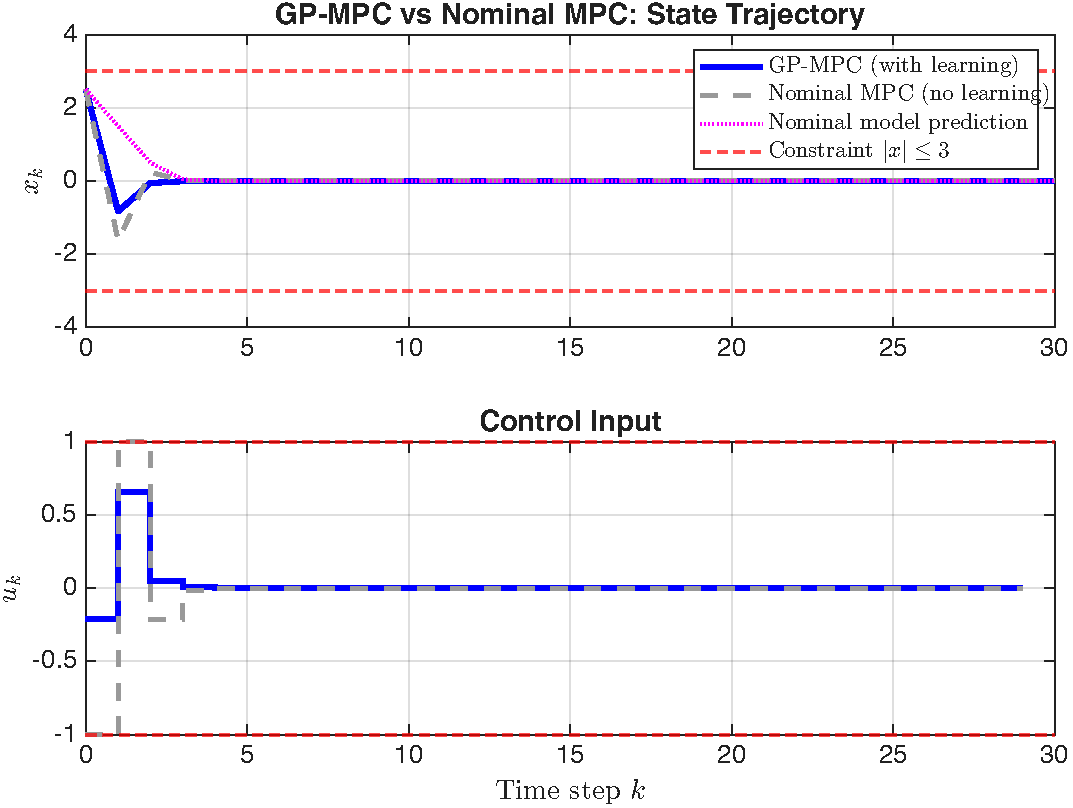
\includegraphics[width=0.88\textwidth]{Figures/fig_gpmpc_simulation.pdf}
	\caption{GP-MPC closed-loop simulation for the scalar system with unknown cubic drag. Top: state trajectory. The GP-MPC controller (blue) drives the state to the origin smoothly, while the nominal controller (grey dashed) exhibits slower convergence due to unmodelled dynamics. Bottom: control input. Both controllers respect the actuator limits $|u_k| \le 1$. The red dashed lines indicate the constraint boundaries.}
	\label{fig:gpmpc_simulation}
\end{figure}

Figure~\ref{fig:gpmpc_architecture} shows the GP-MPC control architecture as a block diagram. The GP model sits alongside the nominal model and feeds both the predicted mean and the predicted variance into the MPC optimisation.

\begin{figure}[ht]
	\centering
	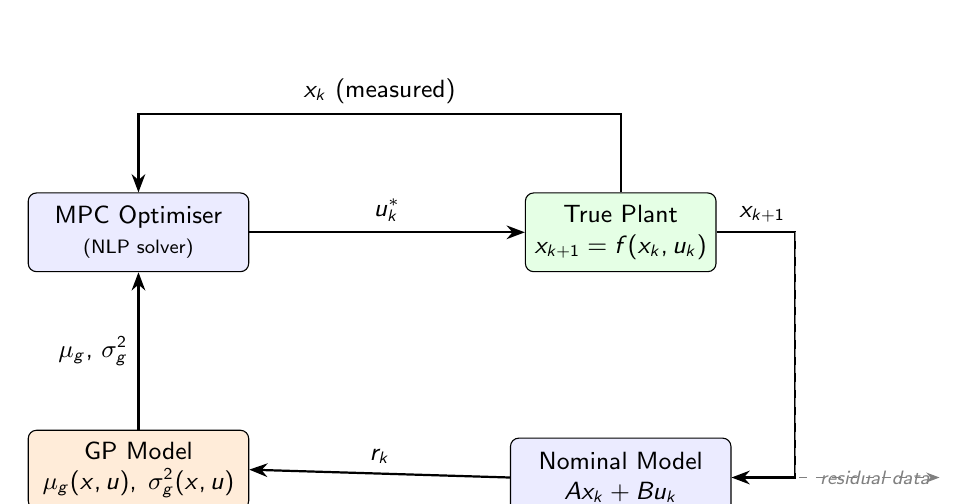
\begin{tikzpicture}[
		>=Stealth,
		node distance=1.0cm and 1.6cm,
		block/.style={draw, rounded corners=3pt, fill=blue!8,
			minimum width=2.8cm, minimum height=1.0cm, align=center, font=\small},
		blockgp/.style={draw, rounded corners=3pt, fill=orange!15,
			minimum width=2.8cm, minimum height=1.0cm, align=center, font=\small},
		blockplant/.style={draw, rounded corners=3pt, fill=green!10,
			minimum width=2.4cm, minimum height=1.0cm, align=center, font=\small},
		sum/.style={draw, circle, minimum size=0.5cm, inner sep=0pt, font=\small},
		arr/.style={->, thick},
	]
		% MPC block
		\node[block] (mpc) {MPC Optimiser\\{\scriptsize (NLP solver)}};

		% Plant
		\node[blockplant, right=3.5cm of mpc] (plant) {True Plant\\$x_{k+1} = f(x_k, u_k)$};

		% GP block
		\node[blockgp, below=2.0cm of mpc] (gp) {GP Model\\$\mu_g(x,u),\; \sigma_g^2(x,u)$};

		% Nominal model
		\node[block, below=2.1cm of plant] (nom) {Nominal Model\\$Ax_k + Bu_k$};

		% Arrows
		\draw[arr] (mpc.east) -- node[above, font=\small] {$u_k^*$} (plant.west);
		\draw[arr] (plant.east) -- ++(1.0,0) node[above left, font=\small] {$x_{k+1}$} |- (nom.east);
		\draw[arr] (nom.west) -- node[above, font=\small] {$r_k$} (gp.east);
		\draw[arr] (gp.north) -- node[left, font=\small] {$\mu_g$, $\sigma_g^2$} (mpc.south);

		% Feedback: x_k to MPC
		\draw[arr] (plant.north) -- ++(0,1.0) -| node[above, pos=0.25, font=\small] {$x_k$ (measured)} (mpc.north);

		% Data collection annotation
		\node[right=1.0cm of nom, font=\scriptsize\itshape, text=gray] (ann) {residual data};
		\draw[->, gray, dashed] (plant.east) ++(1.0,0) |- (ann.east);
	\end{tikzpicture}
	\caption{GP-MPC architecture. At each time step, the measured state $x_k$ is used to query the GP model, which returns the predicted residual mean $\mu_g$ and variance $\sigma_g^2$. These are incorporated into the MPC optimisation as a dynamics correction and as state-dependent constraint tightening, respectively. The residual data $r_k = x_{k+1} - Ax_k - Bu_k$ can optionally be appended to the GP training set for online learning.}
	\label{fig:gpmpc_architecture}
\end{figure}


%% ============================================================
%%  SECTION 3: KOOPMAN OPERATOR AND DATA-DRIVEN LINEAR MODELS
%% ============================================================
\section{Koopman Operator and Data-Driven Linear Models}
\label{sec:koopman}

The GP-MPC approach learns a nonlinear correction to a known model. The Koopman approach takes a fundamentally different route: it transforms the entire nonlinear system into a \emph{linear} one by working in a higher-dimensional space. Once the system is linear, the standard MPC machinery from Chapter~7---quadratic cost, linear constraints, QP solver---applies directly.

\subsection{The Koopman Operator}
\label{sec:koopman_theory}

Consider an autonomous nonlinear system:
\[
x_{k+1} = f(x_k), \qquad x_k \in \mathbb{R}^n
\]
The state evolves in $\mathbb{R}^n$ according to the possibly complicated function $f$. Instead of tracking the state directly, consider tracking \emph{functions of the state}.

An \emph{observable} is any scalar function $\psi \colon \mathbb{R}^n \to \mathbb{R}$. For instance, $\psi(x) = x_1^2 + x_2$ is an observable. If we know $x_k$, we can compute $\psi(x_k)$. One time step later, $\psi$ takes the value $\psi(x_{k+1}) = \psi(f(x_k))$.

\begin{defnbox}{Definition: The Koopman Operator}
	The \emph{Koopman operator} $\mathcal{K}$ acts on observables:
	\[
	(\mathcal{K}\psi)(x) = \psi\bigl(f(x)\bigr)
	\]
	It advances any observable one time step forward along the trajectories of $f$. The crucial property is that $\mathcal{K}$ is \emph{linear}: $\mathcal{K}(\alpha\psi_1 + \beta\psi_2) = \alpha\,\mathcal{K}\psi_1 + \beta\,\mathcal{K}\psi_2$, even when $f$ is nonlinear. The trade-off is that $\mathcal{K}$ acts on a space of \emph{functions}, which is infinite-dimensional.
\end{defnbox}

In other words, nonlinear dynamics of states become \emph{linear dynamics of observables}. If we could find a finite set of observables closed under the action of $\mathcal{K}$, we would have an exact finite-dimensional linear representation of the nonlinear system. For most nonlinear systems, no such finite set exists---but a well-chosen finite dictionary can still produce an accurate approximation.

\subsubsection*{Finite-Dimensional Approximation}

In practice, we choose a \emph{dictionary} of $p$ observables:
\[
\Psi(x) = \begin{bmatrix} \psi_1(x) \\ \psi_2(x) \\ \vdots \\ \psi_p(x) \end{bmatrix} \in \mathbb{R}^p
\]
Common choices include monomials ($x_1$, $x_2$, $x_1^2$, $x_1 x_2$, $x_2^2$, \ldots), radial basis functions, or trigonometric functions. The \emph{lifted state} is $z_k = \Psi(x_k) \in \mathbb{R}^p$, with $p \ge n$. The first $n$ entries are typically chosen to be the original states: $\psi_i(x) = x_i$ for $i = 1, \ldots, n$.

We then seek a matrix $K_d \in \mathbb{R}^{p \times p}$ (we write $K_d$ to distinguish it from the feedback gain $K$ used elsewhere in these notes) such that:
\begin{equation}\label{eq:koopman_approx}
	z_{k+1} = \Psi(x_{k+1}) \approx K_d\,z_k = K_d\,\Psi(x_k)
\end{equation}
This is a \emph{linear} dynamical system in the lifted coordinates $z_k$. The nonlinearity of $f$ is absorbed into the choice of dictionary $\Psi$.

\begin{alertbox}{Dictionary Choice}
	The quality of the approximation~\eqref{eq:koopman_approx} depends entirely on the dictionary $\Psi$. A poor dictionary produces a poor linear model. Common strategies:
	\begin{itemize}[noitemsep]
		\item \emph{Monomials} up to a chosen degree (simple, intuitive, but the number of terms grows combinatorially).
		\item \emph{Radial basis functions} centred at representative states.
		\item \emph{Domain knowledge}: if the nonlinearity involves $x^3$, include $x^3$ in the dictionary.
	\end{itemize}
	There is no universal recipe; choosing a good dictionary remains an open research question.
\end{alertbox}


\subsection{Extended Dynamic Mode Decomposition (EDMD)}
\label{sec:edmd}

EDMD is the standard method for computing the Koopman approximation from data. For a system with control inputs, the dynamics are $x_{k+1} = f(x_k, u_k)$, and the lifted linear model becomes:
\begin{equation}\label{eq:koopman_controlled}
	z_{k+1} \approx A_K\,z_k + B_K\,u_k
\end{equation}

\subsubsection*{The Algorithm}

Collect a trajectory of $T$ state transitions:
\[
\{(x_0, u_0, x_1),\; (x_1, u_1, x_2),\; \ldots,\; (x_{T-2}, u_{T-2}, x_{T-1})\}
\]
Apply the dictionary $\Psi$ to each state:
\begin{align*}
	Z &= \bigl[\Psi(x_0) \;\; \Psi(x_1) \;\; \cdots \;\; \Psi(x_{T-2})\bigr] \in \mathbb{R}^{p \times (T-1)} \\
	Z' &= \bigl[\Psi(x_1) \;\; \Psi(x_2) \;\; \cdots \;\; \Psi(x_{T-1})\bigr] \in \mathbb{R}^{p \times (T-1)} \\
	U &= \bigl[u_0 \;\; u_1 \;\; \cdots \;\; u_{T-2}\bigr] \in \mathbb{R}^{m \times (T-1)}
\end{align*}

The matrices $A_K$ and $B_K$ are found by solving the least-squares problem:
\begin{equation}\label{eq:edmd_ls}
	\bigl[A_K \;\; B_K\bigr] = Z' \begin{bmatrix} Z \\ U \end{bmatrix}^\dagger
\end{equation}
where $\dagger$ denotes the Moore--Penrose pseudoinverse. This minimises $\sum_{k} \|\Psi(x_{k+1}) - A_K\Psi(x_k) - B_K u_k\|^2$.

\begin{examplebox}{Hand-Worked EDMD for a Scalar Nonlinear System}
	\emph{System.} $x_{k+1} = 0.9\,x_k + 0.1\,x_k^2 + u_k$.

	\emph{Dictionary.} $\Psi(x) = [x, \; x^2]^\top$ (two lifted states, $p = 2$).

	We collect 5 transitions from $x_0 = 1$ with inputs $u = [0.1,\; -0.2,\; 0.3,\; -0.1,\; 0.0]$:
	\[
	\begin{array}{c|c|c}
		k & x_k & u_k \\ \hline
		0 & 1.000 & 0.100 \\
		1 & 1.100 & -0.200 \\
		2 & 0.911 & 0.300 \\
		3 & 1.203 & -0.100 \\
		4 & 1.127 & 0.000
	\end{array}
	\]
	where $x_1 = 0.9(1) + 0.1(1)^2 + 0.1 = 1.1$, etc.

	\solution

	\emph{Step 1: Lift the data.}
	\[
	Z = \begin{bmatrix} 1.000 & 1.100 & 0.911 & 1.203 \\ 1.000 & 1.210 & 0.830 & 1.447 \end{bmatrix}, \quad
	Z' = \begin{bmatrix} 1.100 & 0.911 & 1.203 & 1.127 \\ 1.210 & 0.830 & 1.447 & 1.270 \end{bmatrix}
	\]
	\[
	U = \begin{bmatrix} 0.1 & -0.2 & 0.3 & -0.1 \end{bmatrix}
	\]

	\emph{Step 2: Solve.} Form the stacked matrix $\Omega = [Z;\; U] \in \mathbb{R}^{3 \times 4}$ and compute:
	\[
	[A_K \;\; B_K] = Z'\,\Omega^\dagger
	\]
	This yields $A_K \in \mathbb{R}^{2 \times 2}$ and $B_K \in \mathbb{R}^{2 \times 1}$. The resulting $A_K$ captures both the linear and quadratic dynamics in a single linear system.

	\emph{Step 3: Verify.} At $x = 1.5$ with $u = 0$:
	\begin{itemize}[noitemsep]
		\item True: $x^+ = 0.9(1.5) + 0.1(1.5)^2 = 1.575$
		\item Koopman: $z^+ = A_K [1.5,\; 2.25]^\top + B_K \cdot 0$, then extract the first component.
	\end{itemize}
	The predictions should be close, confirming the dictionary captures the quadratic nonlinearity.
\end{examplebox}

The following MATLAB code performs EDMD identification and compares the Koopman prediction to the true dynamics.

\begin{lstlisting}[language=Matlab, caption={EDMD identification for a scalar nonlinear system.}]
% 1. True Nonlinear Plant
f_true = @(x, u) 0.9*x + 0.1*x.^2 + u;

% 2. Data Collection
rng(1);
T = 50;
x_data = zeros(T+1, 1);  x_data(1) = 0;
u_data = 0.5*randn(T, 1);
for k = 1:T
    x_data(k+1) = f_true(x_data(k), u_data(k));
end

% 3. Dictionary: Psi(x) = [x; x^2]
Psi = @(x) [x; x.^2];
p = 2;  % lifted dimension

Z  = zeros(p, T);  Zp = zeros(p, T);
for k = 1:T
    Z(:,k)  = Psi(x_data(k));
    Zp(:,k) = Psi(x_data(k+1));
end
U = u_data(1:T)';

% 4. EDMD: Solve [A_K, B_K] = Zp * [Z; U]'
Omega = [Z; U];
AB = Zp * pinv(Omega);
A_K = AB(:, 1:p);
B_K = AB(:, p+1:end);

% 5. Verify: One-Step Prediction
x_test = linspace(-2, 2, 100);
x_true = f_true(x_test, 0);
x_koop = zeros(1, 100);
for i = 1:100
    z_next = A_K * Psi(x_test(i)) + B_K * 0;
    x_koop(i) = z_next(1);  % extract first component
end

figure; plot(x_test, x_true, 'r-', 'LineWidth', 2); hold on;
plot(x_test, x_koop, 'b--', 'LineWidth', 2);
xlabel('x_k'); ylabel('x_{k+1}');
legend('True dynamics', 'Koopman (EDMD)');
title('EDMD One-Step Prediction (u = 0)'); grid on;
\end{lstlisting}

Figure~\ref{fig:edmd_prediction} compares the Koopman predictor to the true dynamics. The Koopman model (blue dashed) captures the quadratic nonlinearity accurately, while the linearisation about the origin (grey dotted) diverges significantly for $|x| > 1$.

\begin{figure}[ht]
	\centering
	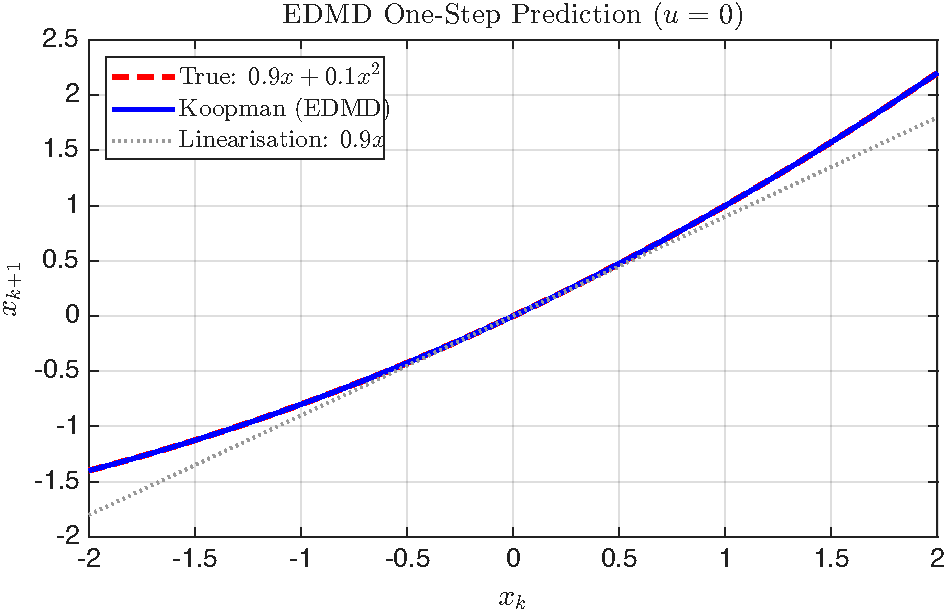
\includegraphics[width=0.82\textwidth]{Figures/fig_edmd_prediction.pdf}
	\caption{EDMD one-step prediction comparison for the scalar system $x_{k+1} = 0.9\,x_k + 0.1\,x_k^2$ (with $u = 0$). The Koopman model identified from 50 data points with dictionary $\Psi(x) = [x,\; x^2]^\top$ closely matches the true nonlinear dynamics (red dashed) --- indeed the two curves overlap almost perfectly, confirming that the dictionary $[x,\; x^2]$ captures the dynamics exactly. The linearisation about the origin (grey dotted, $x_{k+1} \approx 0.9\,x_k$) captures only the linear part and becomes inaccurate away from the origin.}
	\label{fig:edmd_prediction}
\end{figure}


\subsection{Koopman MPC}
\label{sec:koopman_mpc}

With the identified matrices $(A_K, B_K)$, we formulate a standard linear MPC in the lifted coordinates. The optimisation is identical in structure to the one in Chapter~7---it is a QP.

Let $C_x \in \mathbb{R}^{n \times p}$ be the matrix that extracts the original states from the lifted state, i.e.\ $x_k = C_x\,z_k$. Since we chose $\psi_i(x) = x_i$ for $i = 1, \ldots, n$, we simply have $C_x = [I_n \;\; 0]$.

The cost matrices in lifted space are:
\[
\tilde{Q} = C_x^\top Q\,C_x
\]
The terminal cost $\tilde{P}$ is obtained by solving the DARE for the lifted system: $\tilde{P}$ is the stabilising solution of the discrete algebraic Riccati equation with $(A_K, B_K, \tilde{Q}, R)$.

The Koopman MPC problem at time $t$ is:
\begin{equation}\label{eq:koopman_mpc}
	\min_{u_0, \ldots, u_{N-1}} \; \sum_{k=0}^{N-1}\bigl(z_k^\top \tilde{Q}\,z_k + u_k^\top R\,u_k\bigr) + z_N^\top \tilde{P}\,z_N
\end{equation}
subject to:
\begin{align*}
	\text{Initialisation:} \quad & z_0 = \Psi\bigl(x(t)\bigr) \\
	\text{Lifted dynamics:} \quad & z_{k+1} = A_K\,z_k + B_K\,u_k \\
	\text{State constraints:} \quad & x_{\min} \le C_x\,z_k \le x_{\max} \\
	\text{Actuator limits:} \quad & u_{\min} \le u_k \le u_{\max}
\end{align*}

\begin{notebox}{Reusing the Linear MPC Machinery}
	The Koopman MPC problem~\eqref{eq:koopman_mpc} is a standard QP. The YALMIP implementation from Chapter~7 can be reused with minimal changes: replace $A$ with $A_K$, $B$ with $B_K$, $x_k$ with $z_k$, and adjust the cost matrices. The stability theory from Chapter~7---terminal cost, terminal set, recursive feasibility---applies to the \emph{identified Koopman model}. Whether these guarantees transfer to the true nonlinear system depends on the accuracy of the dictionary approximation: a poor dictionary may produce a model whose predictions diverge from the true dynamics, invalidating the stability argument.
\end{notebox}


\subsection{Worked Example: Koopman MPC for a Duffing-Type Oscillator}
\label{sec:koopman_example}

\begin{examplebox}{Koopman MPC for a Nonlinear Oscillator}
	\emph{System.} A Duffing oscillator discretised with RK4 at sampling time $T_s = 0.2$:
	\begin{align*}
		\dot{x}_1 &= x_2, \qquad
		\dot{x}_2 = -x_1 - 3\,x_1^3 - 0.3\,x_2 + u
	\end{align*}
	The strong cubic stiffness ($\beta = 3$) makes this system heavily nonlinear for $|x_1| > 1$.

	\emph{Dictionary.} $\Psi(x) = [x_1,\; x_2,\; x_1^2,\; x_2^2,\; x_1 x_2]^\top$ ($p = 5$ lifted states).

	\emph{Constraints.} $|u_k| \le 2$, $|x_{1,k}| \le 5$ (soft).

	\emph{Objective.} Regulate from $x_0 = [3;\; 0]$ to the origin with $Q = \text{diag}(10, 1)$, $R = 0.1$, $N = 10$.

	\solution

	We collect 1440 data points from 12 diverse initial conditions with random excitation, identify $(A_K, B_K)$ via EDMD, and compare Koopman MPC against linearised MPC using YALMIP. Both controllers use identical MPC formulations; only the prediction model differs.

\begin{lstlisting}[language=Matlab, caption={Koopman MPC vs Linearised MPC for a Duffing oscillator (RK4).}]
% 1. True Nonlinear Plant (RK4 discretisation)
Ts = 0.2;  alpha = 1;  beta = 3;  delta = 0.3;
f_cont = @(x,u) [x(2); -alpha*x(1)-beta*x(1)^3-delta*x(2)+u];
rk4 = @(x,u) rk4_step(f_cont, x, u, Ts);

% Linearisation at origin (numerical Jacobian of RK4 map)
eps_j = 1e-6;
A_lin = zeros(2);
for j = 1:2
    xp = zeros(2,1); xp(j) = eps_j;
    xm = zeros(2,1); xm(j) = -eps_j;
    A_lin(:,j) = (rk4(xp,0)-rk4(xm,0))/(2*eps_j);
end
B_lin = (rk4(zeros(2,1),eps_j)-rk4(zeros(2,1),-eps_j))/(2*eps_j);

% 2. Data Collection (diverse ICs for broad coverage)
rng(42);  nx = 2;
ics = [2 0;-2 0;0 2;0 -2;1.5 1;-1 -1.5;2.5 -1;-2.5 1;
       1 1;-1 1;3 0;-3 0]';
X_all=[];  Xp_all=[];  U_all=[];
for b = 1:size(ics,2)
    x = ics(:,b);
    for k = 1:120
        u = 2.5*randn;  xn = rk4(x, u);
        if any(abs(xn)>10), xn = 0.3*randn(2,1); end
        X_all=[X_all,x]; Xp_all=[Xp_all,xn]; U_all=[U_all,u];
        x = xn;
    end
end

% 3. EDMD Identification
Psi = @(x) [x(1);x(2);x(1)^2;x(2)^2;x(1)*x(2)];
p = 5;  Z = zeros(p,size(X_all,2));  Zp = Z;
for k = 1:size(X_all,2)
    Z(:,k) = Psi(X_all(:,k));  Zp(:,k) = Psi(Xp_all(:,k));
end
AB = Zp * pinv([Z; U_all]);
A_K = AB(:,1:p);  B_K = AB(:,p+1:end);
Cx = [eye(nx), zeros(nx,p-nx)];

% 4. Build Koopman MPC and Linearised MPC (both via YALMIP)
Q = diag([10,1]);  R = 0.1;  N = 10;
u_max = 2;  x1_max = 5;  lam_s = 1e4;
opts = sdpsettings('verbose',0,'solver','quadprog');
Q_lift = Cx'*Q*Cx;

% Koopman MPC
z_par = sdpvar(p,1);  uK = sdpvar(N,1);  sK = sdpvar(N,1);
zp = cell(N+1,1);  zp{1} = z_par;
for k = 1:N, zp{k+1} = A_K*zp{k} + B_K*uK(k); end
objK = 0;  conK = [sK >= 0];
for k = 1:N
    xk = Cx*zp{k+1};
    objK = objK + xk'*Q*xk + R*uK(k)^2 + lam_s*sK(k)^2;
    conK = [conK, -u_max<=uK(k)<=u_max];
    conK = [conK, -x1_max-sK(k)<=xk(1)<=x1_max+sK(k)];
end
koopman_ctrl = optimizer(conK, objK, opts, z_par, uK(1));

% Linearised MPC (same structure, different model)
x_par = sdpvar(nx,1);  uL = sdpvar(N,1);  sL = sdpvar(N,1);
xp = cell(N+1,1);  xp{1} = x_par;
for k = 1:N, xp{k+1} = A_lin*xp{k} + B_lin*uL(k); end
objL = 0;  conL = [sL >= 0];
for k = 1:N
    objL = objL + xp{k+1}'*Q*xp{k+1} + R*uL(k)^2 + lam_s*sL(k)^2;
    conL = [conL, -u_max<=uL(k)<=u_max];
    conL = [conL, -x1_max-sL(k)<=xp{k+1}(1)<=x1_max+sL(k)];
end
linear_ctrl = optimizer(conL, objL, opts, x_par, uL(1));

% 5. Closed-Loop Simulation
T_sim = 60;  x0 = [3; 0];
xK = zeros(nx,T_sim+1); xK(:,1) = x0; uK_h = zeros(1,T_sim);
xL = zeros(nx,T_sim+1); xL(:,1) = x0; uL_h = zeros(1,T_sim);
for t = 1:T_sim
    [uopt,~] = koopman_ctrl(Psi(xK(:,t)));
    uK_h(t) = max(-u_max, min(u_max, full(uopt)));
    xK(:,t+1) = rk4(xK(:,t), uK_h(t));
    [uopt,~] = linear_ctrl(xL(:,t));
    uL_h(t) = max(-u_max, min(u_max, full(uopt)));
    xL(:,t+1) = rk4(xL(:,t), uL_h(t));
end

% Helper: RK4 step
function xn = rk4_step(f, x, u, h)
    k1=f(x,u); k2=f(x+0.5*h*k1,u);
    k3=f(x+0.5*h*k2,u); k4=f(x+h*k3,u);
    xn = x + (h/6)*(k1+2*k2+2*k3+k4);
end
\end{lstlisting}
\end{examplebox}

Figure~\ref{fig:koopman_mpc} compares the two controllers in closed loop. The key difference is visible from the very first time step: at $x_0 = [3;\; 0]$, the linearised controller applies maximum negative input ($u = -2$) because it does not anticipate the strong cubic restoring force. The Koopman controller, which captures this nonlinearity through the lifted dictionary, applies a much smaller input ($u \approx 0.2$) --- it knows the cubic stiffness will pull the state back. Over the full trajectory, Koopman MPC achieves approximately 11\% lower cost and settles roughly 10 steps faster.

\begin{figure}[ht]
	\centering
	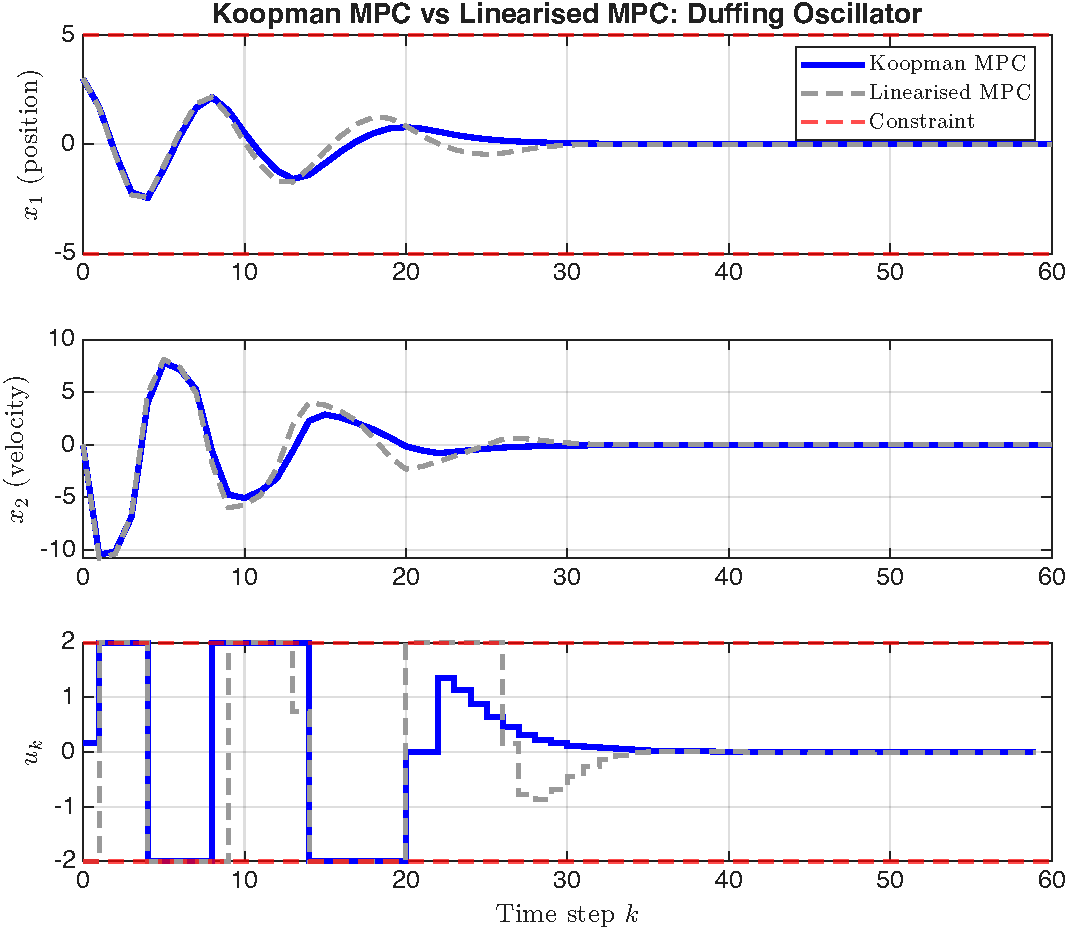
\includegraphics[width=0.88\textwidth]{Figures/fig_koopman_mpc.pdf}
	\caption{Koopman MPC vs linearised MPC for the Duffing oscillator ($\beta = 3$, RK4, $T_s = 0.2$). Top: position $x_1$. Middle: velocity $x_2$. Bottom: control input $u_k$. At $x_0 = [3;\;0]$, the linearised controller (grey dashed) applies maximum effort because it cannot predict the cubic restoring force, leading to larger oscillations. The Koopman controller (blue solid) uses the EDMD-identified lifted model with dictionary $\Psi(x) = [x_1,\; x_2,\; x_1^2,\; x_2^2,\; x_1 x_2]^\top$, exploits the nonlinearity, and settles faster with lower cost.}
	\label{fig:koopman_mpc}
\end{figure}


%% ============================================================
%%  SECTION 4: DATA-ENABLED PREDICTIVE CONTROL (DeePC)
%% ============================================================
\section{Data-Enabled Predictive Control (DeePC)}
\label{sec:deepc}

GP-MPC learns a model correction; Koopman MPC learns a linear representation. Both require an intermediate modelling step. DeePC eliminates this step entirely: raw input--output measurements enter the MPC optimisation directly. The data \emph{is} the model.

The theoretical foundation is \emph{Willems' Fundamental Lemma}, which guarantees that sufficiently rich data from a linear time-invariant (LTI) system captures \emph{all possible} system behaviours.

\subsection{Persistently Exciting Data}
\label{sec:pe}

For data to fully represent a system, the input signal used to collect it must be sufficiently ``rich.'' A constant input reveals nothing about the system's dynamics; a random signal, by contrast, excites all modes.

\begin{defnbox}{Definition: Hankel Matrix}
	Given a signal $\{u_0, u_1, \ldots, u_{T-1}\}$ of length $T$ and a depth $L \le T$, the \emph{Hankel matrix} of depth $L$ is:
	\[
	\mathcal{H}_L(u) = \begin{bmatrix}
		u_0     & u_1     & \cdots & u_{T-L} \\
		u_1     & u_2     & \cdots & u_{T-L+1} \\
		\vdots  &         & \ddots & \vdots \\
		u_{L-1} & u_L     & \cdots & u_{T-1}
	\end{bmatrix} \in \mathbb{R}^{mL \times (T-L+1)}
	\]
	where $m$ is the dimension of $u_k$. Each column is a consecutive length-$L$ window of the signal.
\end{defnbox}

\begin{defnbox}{Definition: Persistence of Excitation}
	A signal $\{u_0, \ldots, u_{T-1}\}$ is \emph{persistently exciting} (PE) of order $L$ if the Hankel matrix $\mathcal{H}_L(u)$ has \emph{full row rank}, i.e.\ $\text{rank}\bigl(\mathcal{H}_L(u)\bigr) = mL$.

	A random signal (e.g.\ $u_k \sim \mathcal{N}(0, \sigma^2)$) is PE of any order with probability one, provided $T$ is large enough. A constant or periodic signal is not PE of high order.
\end{defnbox}

\subsection{Willems' Fundamental Lemma}
\label{sec:willems}

We now state the central result that underpins DeePC.

Let $(u^d, y^d) = \{(u_0^d, y_0^d), (u_1^d, y_1^d), \ldots, (u_{T-1}^d, y_{T-1}^d)\}$ be a single input--output trajectory of length $T$ collected from an LTI system of order $n$ (i.e.\ the system has $n$ states). Construct the stacked Hankel matrix:
\[
\mathcal{H}_L\!\binom{u^d}{y^d} = \begin{bmatrix} \mathcal{H}_L(u^d) \\ \mathcal{H}_L(y^d) \end{bmatrix}
\]

\begin{defnbox}{Willems' Fundamental Lemma~\cite{Willems2005}}
	Assume the LTI system is \emph{controllable} (i.e.\ the pair $(A, B)$ has full rank controllability matrix). If $u^d$ is persistently exciting of order $L + n$, then $(u, y)$ is a valid length-$L$ input--output trajectory of the system \emph{if and only if} there exists a vector $g \in \mathbb{R}^{T-L+1}$ such that:
	\begin{equation}\label{eq:fundamental_lemma}
		\begin{bmatrix} \mathcal{H}_L(u^d) \\ \mathcal{H}_L(y^d) \end{bmatrix} g = \begin{bmatrix} u \\ y \end{bmatrix}
	\end{equation}
\end{defnbox}

The PE order is $L + n$ rather than $L$ alone because the extra $n$ rows are needed to span the $n$-dimensional initial state space on top of the $L$-step trajectory space. Controllability ensures that all modes can be reached by the input.

In plain language: the columns of the stacked Hankel matrix span every possible length-$L$ trajectory the system can produce. To generate any specific trajectory $(u, y)$, we find a linear combination $g$ of the data columns. The vector $g$ is not a physical quantity---it is simply the ``recipe'' for combining stored data windows.

\begin{examplebox}{Verifying the Fundamental Lemma}
	\emph{System.} A first-order system: $x_{k+1} = 0.8\,x_k + u_k$, $y_k = x_k$, so $n = 1$.

	We collect $T = 10$ data points with input $u^d = [0.5,\; -1.2,\; 0.3,\; 0.8,\; -0.6,\; 1.1,\; -0.4,\; 0.7,\; -0.9,\; 0.2]$ starting from $x_0 = 0$. The corresponding output $y^d$ is computed from the recursion.

	\solution

	Choose $L = 3$. The PE condition requires $u^d$ to be PE of order $L + n = 4$. The Hankel matrix $\mathcal{H}_4(u^d) \in \mathbb{R}^{4 \times 7}$ must have rank~4. For a random-like input with $T = 10$, this is easily satisfied.

	Construct the stacked Hankel matrix $\mathcal{H}_3\binom{u^d}{y^d} \in \mathbb{R}^{6 \times 8}$.

	Now pick any valid 3-step trajectory. For instance, start from $x_0 = 1$ with $u = [0.5,\; -0.3,\; 0.1]$. Compute $y = [1.0,\; 1.3,\; 0.74]$ from the recursion. Then find $g$ such that~\eqref{eq:fundamental_lemma} holds by solving the (overdetermined) linear system. If the data is PE, a solution $g$ exists.

\begin{lstlisting}[language=Matlab, caption={Verifying Willems' Fundamental Lemma.}]
% 1. System
a = 0.8;  b = 1;  n = 1;

% 2. Data Collection
ud = [0.5, -1.2, 0.3, 0.8, -0.6, 1.1, -0.4, 0.7, -0.9, 0.2];
T = length(ud);
xd = zeros(1, T+1);  xd(1) = 0;
for k = 1:T
    xd(k+1) = a*xd(k) + b*ud(k);
end
yd = xd(1:T);  % y_k = x_k

% 3. Build Hankel Matrices (depth L = 3)
L = 3;
Hu = zeros(L, T-L+1);  Hy = zeros(L, T-L+1);
for j = 1:T-L+1
    Hu(:,j) = ud(j:j+L-1)';
    Hy(:,j) = yd(j:j+L-1)';
end
H = [Hu; Hy];  % stacked Hankel matrix (6 x 8)

% 4. Check PE: rank of H_4(u^d) must be 4
Hu4 = zeros(L+n, T-L-n+1);
for j = 1:T-L-n+1
    Hu4(:,j) = ud(j:j+L+n-1)';
end
fprintf('Rank of H_%d(u^d) = %d (need %d)\n', L+n, rank(Hu4), L+n);

% 5. Recover a Known Trajectory
x_test = zeros(1, L+1);  x_test(1) = 1.0;
u_test = [0.5, -0.3, 0.1];
for k = 1:L
    x_test(k+1) = a*x_test(k) + b*u_test(k);
end
y_test = x_test(1:L);

traj = [u_test'; y_test'];
g = H \ traj;       % solve H * g = [u; y]
traj_recovered = H * g;

fprintf('Target trajectory:    [%s]\n', num2str(traj', '%8.4f'));
fprintf('Recovered trajectory: [%s]\n', num2str(traj_recovered', '%8.4f'));
\end{lstlisting}
\end{examplebox}


\subsection{The DeePC Optimisation Problem}
\label{sec:deepc_formulation}

We now use the Fundamental Lemma to build a predictive controller. The key step is to partition the Hankel matrix into \emph{past} and \emph{future} blocks.

Set $L = T_\text{ini} + N$, where:
\begin{itemize}[noitemsep]
	\item $T_\text{ini}$ is the number of past time steps used to ``initialise'' the prediction (replaces the state $x_0$ in model-based MPC).
	\item $N$ is the prediction horizon (same role as in Chapter~7).
\end{itemize}

Partition the Hankel data as:
\begin{equation}\label{eq:deepc_partition}
	\begin{bmatrix} U_p \\ Y_p \\ U_f \\ Y_f \end{bmatrix} g = \begin{bmatrix} u_\text{ini} \\ y_\text{ini} \\ u \\ y \end{bmatrix}
\end{equation}
where $U_p, Y_p \in \mathbb{R}^{mT_\text{ini} \times \cdot}$ are the past blocks and $U_f, Y_f \in \mathbb{R}^{mN \times \cdot}$ are the future blocks. The vectors $u_\text{ini}$ and $y_\text{ini}$ are the most recent $T_\text{ini}$ measurements from the real system.

\begin{alertbox}{$T_\text{ini}$ replaces the state}
	In model-based MPC, the current state $x_0 = x(t)$ is measured (or estimated). DeePC does not use a state. Instead, the past $T_\text{ini}$ input--output measurements pin the initial condition. For an $n$th-order system, $T_\text{ini} \ge n$ is required to uniquely determine the internal state from input--output data. In practice, use $T_\text{ini} = n$ or slightly larger.
\end{alertbox}

The \emph{DeePC optimisation} at each time step is:
\begin{equation}\label{eq:deepc_qp}
	\min_{g,\, \sigma_y} \; \sum_{k=0}^{N-1}\bigl(\|y_{f,k} - y_\text{ref}\|_Q^2 + \|u_{f,k}\|_R^2\bigr) \;+\; \lambda_g\,\|g\|_1 \;+\; \lambda_\sigma\,\|\sigma_y\|_2^2
\end{equation}
subject to:
\begin{align*}
	\text{Data consistency:} \quad & \begin{bmatrix} U_p \\ Y_p \\ U_f \\ Y_f \end{bmatrix} g = \begin{bmatrix} u_\text{ini} \\ y_\text{ini} + \sigma_y \\ u \\ y \end{bmatrix} \\[4pt]
	\text{Output constraints:} \quad & y_{\min} \le y_{f,k} \le y_{\max}, \quad k = 0, \ldots, N-1 \\
	\text{Input constraints:} \quad & u_{\min} \le u_{f,k} \le u_{\max}, \quad k = 0, \ldots, N-1
\end{align*}

The two \emph{regularisation terms} are critical for noisy data:
\begin{itemize}
	\item $\lambda_g\|g\|_1$ promotes \emph{sparsity} in the data-selection vector $g$: only a few columns of the Hankel matrix are active. This selects the most relevant data windows and suppresses noisy or irrelevant ones.
	\item $\lambda_\sigma\|\sigma_y\|_2^2$ penalises the slack variable $\sigma_y$ on the past output match. With noisy measurements, an exact match to the past outputs forces $g$ to ``explain'' the noise, degrading the prediction. The quadratic penalty keeps the slack small while absorbing measurement noise smoothly.
\end{itemize}

\begin{defnbox}{DeePC as implicit system identification}
	The $\ell_1$ penalty on $g$ promotes sparsity: as $\lambda_g$ increases, fewer Hankel columns are selected. For LTI systems with noise-free data, the Fundamental Lemma guarantees that any single consistent column suffices to represent the trajectory, so the sparse solution selects the most relevant data windows. In the noisy case, the interplay between $\lambda_g$ and $\lambda_\sigma$ balances data fidelity against noise rejection~\cite{Dorfler2023}. This equivalence holds under the LTI assumption; for nonlinear systems, the connection does not carry over.
\end{defnbox}

\subsection{Worked Example: DeePC for a Scalar Integrator (Hand-Worked)}
\label{sec:deepc_scalar}

\begin{examplebox}{DeePC for a Scalar Integrator}
	\emph{System.} $y_{k+1} = y_k + u_k$ (order $n = 1$, SISO).

	\emph{Data.} $T = 8$ samples with PE input $u^d = [1,\; -1,\; 0.5,\; -0.5,\; 1,\; -1,\; 0.5,\; -0.5]$, starting from $y_0^d = 0$:
	\[
	y^d = [0,\; 1,\; 0,\; 0.5,\; 0,\; 1,\; 0,\; 0.5]
	\]

	\emph{Parameters.} $T_\text{ini} = 1$, $N = 2$, $Q = 1$, $R = 0.1$, $\lambda_g = 0$, $\lambda_\sigma = 0$ (noise-free).

	\solution

	$L = T_\text{ini} + N = 3$. Construct the $3 \times 6$ Hankel matrices and partition into past (1 row) and future (2 rows):
	\begin{align*}
		U_p &= \begin{bmatrix} 1 & -1 & 0.5 & -0.5 & 1 & -1 \end{bmatrix} \\
		U_f &= \begin{bmatrix} -1 & 0.5 & -0.5 & 1 & -1 & 0.5 \\ 0.5 & -0.5 & 1 & -1 & 0.5 & -0.5 \end{bmatrix}
	\end{align*}
	and similarly for $Y_p$, $Y_f$ from $y^d$.

	At time $t$, suppose the most recent measurement is $y_\text{ini} = 2$ and $u_\text{ini} = 0$. The DeePC QP~\eqref{eq:deepc_qp} is:
	\[
	\min_{g \in \mathbb{R}^6}\; (y_{f,1} - 0)^2 + (y_{f,2} - 0)^2 + 0.1\,u_{f,1}^2 + 0.1\,u_{f,2}^2
	\]
	subject to the Hankel constraint~\eqref{eq:deepc_partition} with the past block pinning $u_\text{ini} = 0$, $y_\text{ini} = 2$.

	Solving this QP yields future inputs $u_{f,1}^*$ and $u_{f,2}^*$, and the controller applies $u_0^* = u_{f,1}^*$. The result is the same as model-based MPC for this LTI system, confirming the Fundamental Lemma.
\end{examplebox}


\subsection{Worked Example: DeePC for a Double Integrator with Constraints}
\label{sec:deepc_double_int}

\begin{examplebox}{DeePC for a Double Integrator}
	\emph{System.} The same double integrator used in Chapters~5, 7 and the Tube MPC chapter:
	\[
	A = \begin{bmatrix} 1 & 1 \\ 0 & 1 \end{bmatrix}, \quad B = \begin{bmatrix} 0.5 \\ 1 \end{bmatrix}, \quad C = \begin{bmatrix} 1 & 0 \end{bmatrix}
	\]
	The output $y_k = x_{1,k}$ is the position. The system has order $n = 2$.

	\emph{Constraints.} $|u_k| \le 1$, $|y_k| \le 5$.

	\emph{Parameters.} $T = 200$ data samples, $T_\text{ini} = 2$, $N = 10$, $Q = 1$, $R = 0.1$, $\lambda_g = 100$, $\lambda_\sigma = 10^4$.

	\solution

\begin{lstlisting}[language=Matlab, caption={DeePC for a constrained double integrator.}]
% 1. Data Collection (persistently exciting input)
A = [1 1; 0 1];  B = [0.5; 1];  C = [1 0];
nx = 2; nu = 1; ny = 1; n_order = 2;
rng(3);
T = 200;
x_sim = zeros(nx, T+1);
u_d = randn(1, T);   % PE input
y_d = zeros(1, T);
for k = 1:T
    y_d(k) = C * x_sim(:,k);
    x_sim(:,k+1) = A * x_sim(:,k) + B * u_d(k);
end

% 2. Hankel Matrix Construction
Tini = 2;  N = 10;  L = Tini + N;
n_col = T - L + 1;

Hu = zeros(L, n_col);  Hy = zeros(L, n_col);
for j = 1:n_col
    Hu(:,j) = u_d(j:j+L-1)';
    Hy(:,j) = y_d(j:j+L-1)';
end

% Partition into past / future
Up = Hu(1:Tini, :);       Yp = Hy(1:Tini, :);
Uf = Hu(Tini+1:end, :);   Yf = Hy(Tini+1:end, :);

% 3. DeePC Optimisation via YALMIP
Q_cost = 1;  R_cost = 0.1;
lam_g = 100;  lam_sig = 1e4;
u_max = 1;    y_max = 5;

g      = sdpvar(n_col, 1);
sig_y  = sdpvar(Tini, 1);
u_ini  = sdpvar(Tini, 1);
y_ini  = sdpvar(Tini, 1);

u_f = Uf * g;  y_f = Yf * g;

con = [Up * g == u_ini];
con = [con, Yp * g == y_ini + sig_y];
con = [con, -u_max <= u_f <= u_max];
con = [con, -y_max <= y_f <= y_max];

obj = 0;
for k = 1:N
    obj = obj + Q_cost * y_f(k)^2 + R_cost * u_f(k)^2;
end
obj = obj + lam_g * norm(g, 1) + lam_sig * (sig_y' * sig_y);

opts = sdpsettings('verbose', 0, 'solver', 'quadprog');
deepc = optimizer(con, obj, opts, {u_ini, y_ini}, u_f(1));

% 4. Receding-Horizon Simulation
T_sim = 40;
x_state = [4; 0];  % initial condition
x_hist = zeros(nx, T_sim+1);  x_hist(:,1) = x_state;
u_hist = zeros(1, T_sim);     y_hist = zeros(1, T_sim);

% Past buffers (initialise with zeros)
u_buf = zeros(Tini, 1);
y_buf = zeros(Tini, 1);
y_buf(end) = C * x_state;

for t = 1:T_sim
    [u_opt, errcode] = deepc({u_buf, y_buf});
    if errcode ~= 0, warning('DeePC infeasible at t=%d', t); end
    u_hist(t) = u_opt;
    y_hist(t) = C * x_state;

    x_state = A * x_state + B * u_opt;
    x_hist(:,t+1) = x_state;

    % Shift past buffers
    u_buf = [u_buf(2:end); u_opt];
    y_buf = [y_buf(2:end); C * x_state];
end

% 5. Plot
figure;
subplot(2,1,1); plot(0:T_sim, x_hist(1,:), 'b', 'LineWidth', 2);
yline(y_max,'r--','LineWidth',1.5); yline(-y_max,'r--','LineWidth',1.5);
ylabel('y_k = x_1'); title('DeePC: Output'); grid on;
subplot(2,1,2); stairs(0:T_sim-1, u_hist, 'b', 'LineWidth', 2);
yline(u_max,'r--','LineWidth',1.5); yline(-u_max,'r--','LineWidth',1.5);
ylabel('u_k'); xlabel('Time step k'); title('DeePC: Control'); grid on;
\end{lstlisting}
\end{examplebox}

\begin{alertbox}{Data Requirements}
	The PE condition requires $T \ge (m+1)(L + n) - 1$. For the double integrator ($n=2$, $m=1$) with $L = T_\text{ini} + N = 12$: $T \ge 2 \times 14 - 1 = 27$. We use $T = 200$, which is well above this minimum. More data improves robustness to noise, at the cost of larger Hankel matrices and slower QP solves.
\end{alertbox}

\begin{summarybox}{DeePC Design Checklist}
	\begin{enumerate}
		\item Collect input--output data with a persistently exciting input. Ensure $T \ge (m+1)(L + n) - 1$.
		\item Choose $T_\text{ini} \ge n$ (the system order, or a conservative estimate).
		\item Choose the prediction horizon $N$ (same considerations as Chapter~7).
		\item Construct the Hankel matrices and partition into past / future blocks.
		\item Select regularisation weights: start with $\lambda_g \approx 100$ and $\lambda_\sigma \approx 10^4$, then tune.
		\item At each step, fill the past buffers $u_\text{ini}$, $y_\text{ini}$ from recent measurements, solve the QP, apply $u_0^*$, and shift the buffers.
	\end{enumerate}
\end{summarybox}

Figure~\ref{fig:deepc_simulation} compares DeePC to model-based MPC. Both controllers regulate the output to the origin while respecting constraints. The DeePC controller exhibits slightly more oscillatory control action due to the finite data and regularisation, but successfully stabilises the system using only input--output data.

\begin{figure}[ht]
	\centering
	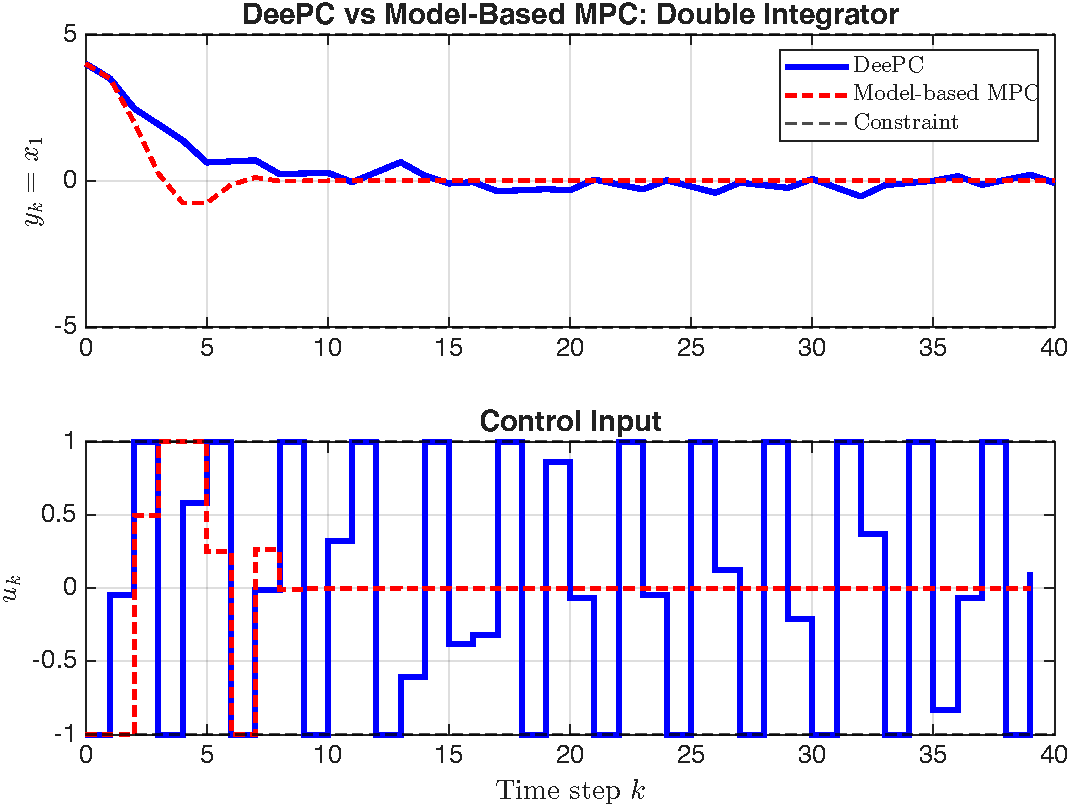
\includegraphics[width=0.88\textwidth]{Figures/fig_deepc_simulation.pdf}
	\caption{DeePC vs model-based MPC for the constrained double integrator. Top: output $y_k = x_1$ regulated from $y_0 = 4$ to the origin. Bottom: control input. The DeePC controller (blue solid) uses 200 data points and Hankel-matrix predictions; the model-based controller (red dashed) uses the known state-space model. Both respect the constraints $|u_k| \le 1$, $|y_k| \le 5$. The DeePC controller shows slightly more aggressive control switching due to finite-data effects and regularisation, while the model-based controller produces a smoother response.}
	\label{fig:deepc_simulation}
\end{figure}

Figure~\ref{fig:deepc_architecture} illustrates the DeePC control loop. The key distinction from model-based MPC is that no system matrices appear anywhere---the Hankel matrices built from raw data serve as the prediction engine.

\begin{figure}[ht]
	\centering
	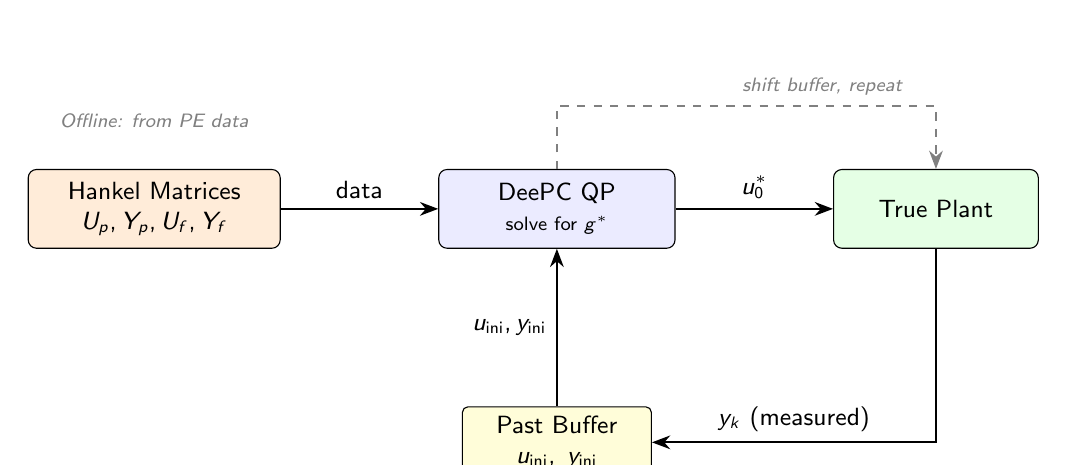
\begin{tikzpicture}[
		>=Stealth,
		node distance=1.0cm and 1.5cm,
		block/.style={draw, rounded corners=3pt, fill=blue!8,
			minimum width=3.0cm, minimum height=1.0cm, align=center, font=\small},
		blockdata/.style={draw, rounded corners=3pt, fill=orange!15,
			minimum width=3.2cm, minimum height=1.0cm, align=center, font=\small},
		blockplant/.style={draw, rounded corners=3pt, fill=green!10,
			minimum width=2.6cm, minimum height=1.0cm, align=center, font=\small},
		buf/.style={draw, rounded corners=2pt, fill=yellow!15,
			minimum width=2.4cm, minimum height=0.8cm, align=center, font=\small},
		arr/.style={->, thick},
	]
		% Data collection (offline)
		\node[blockdata] (hankel) {Hankel Matrices\\$U_p, Y_p, U_f, Y_f$};
		\node[above=0.4cm of hankel, font=\scriptsize\itshape, text=gray] {Offline: from PE data};

		% DeePC QP
		\node[block, right=2.0cm of hankel] (qp) {DeePC QP\\{\scriptsize solve for $g^*$}};

		% Plant
		\node[blockplant, right=2.0cm of qp] (plant) {True Plant};

		% Past buffer
		\node[buf, below=2.0cm of qp] (buf) {Past Buffer\\$u_\text{ini},\; y_\text{ini}$};

		% Arrows
		\draw[arr] (hankel.east) -- node[above, font=\small] {data} (qp.west);
		\draw[arr] (qp.east) -- node[above, font=\small] {$u_0^*$} (plant.west);
		\draw[arr] (plant.south) -- (plant.south |- buf.east) -- node[above, font=\small] {$y_k$ (measured)} (buf.east);
		\draw[arr] (buf.north) -- node[left, font=\small] {$u_\text{ini}, y_\text{ini}$} (qp.south);

		% Receding horizon annotation
		\draw[arr, dashed, gray] (qp.north) -- ++(0,0.8) -| node[above, pos=0.35, font=\scriptsize\itshape, text=gray] {shift buffer, repeat} (plant.north);
	\end{tikzpicture}
	\caption{DeePC receding-horizon control loop. The Hankel matrices are built once from a persistently exciting offline experiment. At each online step, the past input--output buffer $(u_\text{ini}, y_\text{ini})$ is fed into the DeePC QP along with the Hankel data. The QP finds the optimal combination vector $g^*$, from which the first future input $u_0^*$ is applied to the plant. After measuring the new output, the past buffer is shifted forward and the process repeats.}
	\label{fig:deepc_architecture}
\end{figure}

\subsection{Practical Considerations}
\label{sec:deepc_practical}

For nonlinear systems, the Fundamental Lemma does not hold---the Hankel columns span only LTI behaviours. Workarounds include short rolling data windows (re-collecting data periodically), strong regularisation ($\lambda_g \gg 0$), and multiple shooting with data-driven predictors.

Figure~\ref{fig:deepc_noise} illustrates how measurement noise degrades DeePC performance. As the noise level $\sigma$ increases, the closed-loop trajectory degrades---highlighting the importance of regularisation ($\lambda_g$, $\lambda_\sigma$) when working with noisy data.

\begin{figure}[ht]
	\centering
	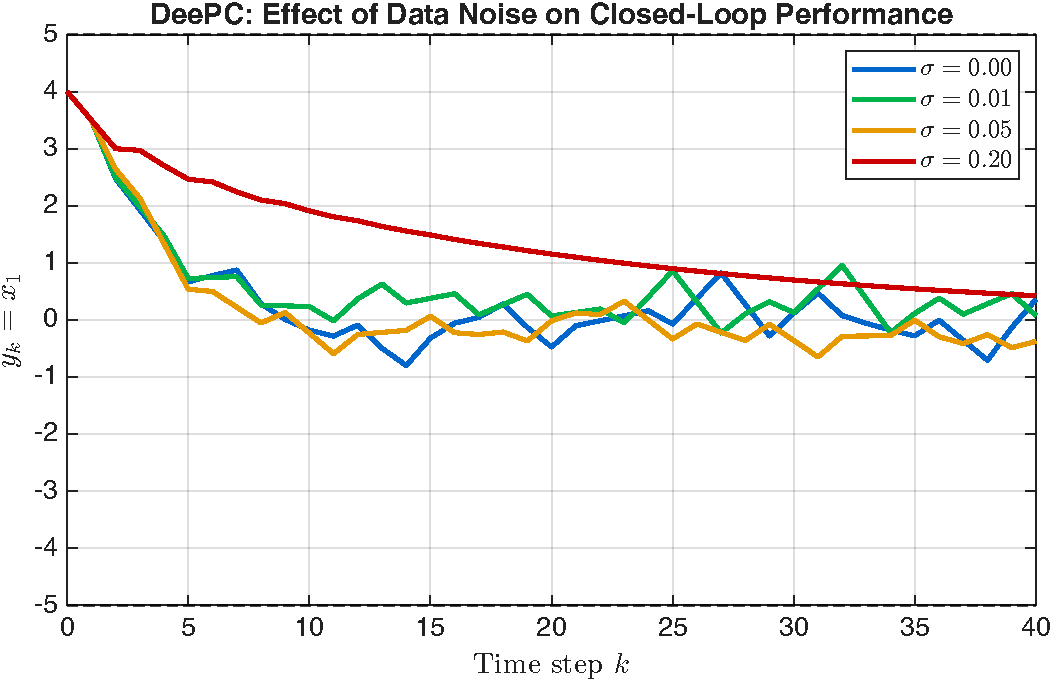
\includegraphics[width=0.85\textwidth]{Figures/fig_deepc_noise.pdf}
	\caption{DeePC noise sensitivity study for the double integrator. Four noise levels are compared: $\sigma = 0$ (noise-free, blue), $\sigma = 0.01$ (green), $\sigma = 0.05$ (orange), and $\sigma = 0.20$ (red). The regularisation weight $\lambda_g$ is scaled with the noise level. At low noise, DeePC closely matches model-based MPC. As noise increases, the Hankel data becomes less representative of the true system, causing slower convergence and larger tracking errors. Data quality and regularisation tuning are essential for reliable DeePC performance.}
	\label{fig:deepc_noise}
\end{figure}


%% ============================================================
%%  SECTION 5: LEARNING MPC (LMPC)
%% ============================================================
\section{Learning MPC}
\label{sec:lmpc}

The methods above learn a model (GP-MPC, Koopman) or bypass it (DeePC) using offline data. Learning MPC (LMPC) takes a different approach: it learns from \emph{repeated executions of the same task}, improving the controller with each iteration.

\subsection{The Iterative Task Setting}
\label{sec:lmpc_setting}

\begin{defnbox}{Definition: Iterative Task}
	A task is \emph{iterative} if the system must repeatedly drive from a fixed initial state $x_S$ to a fixed terminal state $x_F$, under the same dynamics $x_{k+1} = f(x_k, u_k)$ and the same constraints $x_k \in \mathcal{X}$, $u_k \in \mathcal{U}$.
\end{defnbox}

Motivating examples:
\begin{itemize}[noitemsep]
	\item \emph{Autonomous racing.} A car completes laps on the same track. Each lap is an iteration.
	\item \emph{Pick-and-place robots.} A robotic arm repeatedly moves objects between the same two positions.
	\item \emph{Batch chemical processes.} The same reaction is run repeatedly, aiming for a target yield.
\end{itemize}

We index iterations by $j = 0, 1, 2, \ldots$ and time steps within an iteration by $k = 0, 1, \ldots, T_j$, where $T_j$ is the time at which iteration $j$ terminates (i.e.\ $x_{T_j}^{(j)} = x_F$). The trajectory at iteration $j$ is $\{x_0^{(j)}, u_0^{(j)}, x_1^{(j)}, u_1^{(j)}, \ldots, x_{T_j}^{(j)}\}$.


\subsection{Safe Set and Terminal Cost from Data}
\label{sec:lmpc_safe_set}

After $j$ successful iterations, we have $j+1$ complete trajectories (iterations $0, 1, \ldots, j$) that all satisfy the constraints and reach the target. The union of \emph{every state visited during any of these iterations} forms the \emph{sampled safe set}:
\begin{equation}\label{eq:safe_set}
	\mathcal{SS}^j = \bigcup_{i=0}^{j}\bigl\{x_0^{(i)},\; x_1^{(i)},\; \ldots,\; x_{T_i}^{(i)}\bigr\}
\end{equation}
Here $x_k^{(i)}$ denotes the state at time step $k$ during iteration $i$, and $T_i$ is the number of steps iteration $i$ took to reach the target. The superscript $(i)$ always refers to the iteration index and the subscript to the time index within that iteration. Since every iteration reached $x_F$ safely, every state in $\mathcal{SS}^j$ is a state from which the target is \emph{known to be reachable} without violating constraints --- hence the name ``safe set.'' As we complete more iterations, $\mathcal{SS}^j$ can only grow: $\mathcal{SS}^{j} \supseteq \mathcal{SS}^{j-1}$.

For each state in $\mathcal{SS}^j$, we can compute the \emph{cost-to-go}: the total cost that was actually incurred from that state to the target during the iteration in which it was visited. If the same state $x$ was visited during multiple iterations, we take the cheapest one:
\begin{equation}\label{eq:cost_to_go}
	Q^j(x) = \min_{(i,k):\, x_k^{(i)} = x}\; \sum_{t=k}^{T_i} \ell\bigl(x_t^{(i)},\, u_t^{(i)}\bigr)
\end{equation}
The minimum is over all (iteration, time step) pairs $(i,k)$ for which the system was in state $x$ at step $k$ of iteration $i$. The sum counts the stage costs from that point onwards until the end of that iteration. For example, if $\ell = 1$ (minimum-time), then $Q^j(x_k^{(i)}) = T_i - k$: the number of remaining steps. If the same state appeared in a later, faster iteration, $Q^j$ takes the smaller value.

The LMPC optimisation at iteration $j+1$ is:
\begin{equation}\label{eq:lmpc_opt}
	\min_{u_0, \ldots, u_{N-1}}\; \sum_{k=0}^{N-1}\ell(x_k, u_k) + Q^j(x_N)
\end{equation}
subject to:
\begin{align*}
	\text{Initialisation:} \quad & x_0 = x(t) \\
	\text{Dynamics:} \quad & x_{k+1} = f(x_k, u_k) \\
	\text{Constraints:} \quad & x_k \in \mathcal{X}, \quad u_k \in \mathcal{U} \\
	\text{Terminal constraint:} \quad & x_N \in \text{conv}(\mathcal{SS}^j)
\end{align*}
where $\text{conv}(\mathcal{SS}^j)$ denotes the convex hull of the sampled safe set. In practice, the terminal constraint is implemented via convex combination variables: $x_N = \sum_{(i,k)} \lambda_k^{(i)}\,x_k^{(i)}$, with $\lambda_k^{(i)} \ge 0$ and $\sum \lambda = 1$. The terminal cost is interpolated accordingly: $Q^j(x_N) = \sum \lambda_k^{(i)}\,Q^j(x_k^{(i)})$. This convex-hull relaxation is essential---constraining $x_N$ to lie in the \emph{finite} set $\mathcal{SS}^j$ exactly would make the problem combinatorial. For linear systems, the convex hull preserves feasibility; for nonlinear systems, the safe set is used as a lookup table with nearest-neighbour matching as in the worked example below.

\begin{notebox}{Connection to Terminal Sets (Chapter~7)}
	In standard MPC, the terminal set $\mathcal{X}_f$ and terminal cost $V_f(x)$ are computed offline from the model (typically via the DARE and the maximal positive invariant set). In LMPC, both are built from data:
	\begin{itemize}[noitemsep]
		\item $\mathcal{SS}^j$ plays the role of $\mathcal{X}_f$---it is a set of states from which the target is known to be reachable.
		\item $Q^j(x)$ plays the role of $V_f(x)$---it is a valid upper bound on the true cost-to-go.
	\end{itemize}
	As $j$ grows, $\mathcal{SS}^j$ expands and $Q^j$ decreases, so the controller has more freedom and achieves better performance.
\end{notebox}

\subsection{Guarantees}
\label{sec:lmpc_guarantees}

LMPC provides two important properties without requiring an explicit model:

\emph{Recursive feasibility.} If iteration $j$ was feasible (the system reached $x_F$), then iteration $j+1$ is also feasible. The argument has two parts: (i)~\emph{inter-iteration}: the trajectory from iteration $j$ is contained in $\mathcal{SS}^j$, so it is available as a feasible candidate for iteration $j+1$; (ii)~\emph{intra-iteration}: at each time step within iteration $j+1$, the standard shifted-sequence argument applies---the tail of the previous solution provides a feasible candidate, and its terminal state remains in $\mathcal{SS}^j$ because all successor states from previous iterations are already in the safe set.

\emph{Non-increasing cost.} $J^{(j+1)} \le J^{(j)}$. Since the previous trajectory is feasible, the optimal cost at iteration $j+1$ is at most the cost of the previous trajectory. Strict improvement occurs when the expanded safe set opens up shorter or cheaper paths.

The cost sequence $\{J^{(j)}\}$ is non-increasing and bounded below (by zero), so it converges. For convex problems, convergence is to the global optimum; for nonlinear systems, LMPC may converge to a local optimum depending on the initial trajectory and the horizon $N$.


\subsection{Worked Example: LMPC for a Scalar Minimum-Time Problem}
\label{sec:lmpc_example}

\begin{examplebox}{LMPC: Scalar Minimum-Time Problem}
	\emph{System.} $x_{k+1} = x_k + u_k$, with $|u_k| \le 0.5$.

	\emph{Task.} Drive from $x_0 = 2$ to $x_F = 0$ in minimum time (stage cost $\ell = 1$ per step).

	\emph{Iteration 0: conservative controller.} Use $u_k = -0.3$ (well within the constraint) at every step.
	\[
	\begin{array}{c|c c c c c c c c}
		k & 0 & 1 & 2 & 3 & 4 & 5 & 6 & 7 \\
		\hline
		x_k^{(0)} & 2.0 & 1.7 & 1.4 & 1.1 & 0.8 & 0.5 & 0.2 & -0.1
	\end{array}
	\]
	Cost: $J^{(0)} = 7$ steps.

	\solution

	\emph{Build $\mathcal{SS}^0$ and $Q^0$.} The safe set is $\{2.0,\; 1.7,\; 1.4,\; 1.1,\; 0.8,\; 0.5,\; 0.2,\; 0\}$. The cost-to-go from each state is the number of remaining steps: $Q^0(2.0) = 7$, $Q^0(1.7) = 6$, \ldots, $Q^0(0) = 0$.

	\emph{Iteration 1: LMPC.} With $N = 3$, the LMPC plans from $x_0 = 2$ and requires $x_3 \in \mathcal{SS}^0$. Since the constraint allows $u = -0.5$, the optimiser can reach $x_3 = 0.5$ in 3 steps (using $u = -0.5$ each time). The cost-to-go from $x_3 = 0.5$ is $Q^0(0.5) = 2$, so the planned total cost is $3 + 2 = 5$. This is less than $J^{(0)} = 7$.

	After completing iteration 1, the safe set $\mathcal{SS}^1$ is expanded with the new states, and the cost-to-go $Q^1$ is updated with the lower costs observed.

	\emph{Iteration 2 and beyond.} The safe set grows, the cost-to-go improves, and LMPC converges to the optimal solution: $u_k = -0.5$ for 4 steps, reaching $x_F = 0$ in minimum time $T^* = 4$.

\begin{lstlisting}[language=Matlab, caption={LMPC for scalar minimum-time regulation.}]
% 1. System and Constraints
f = @(x, u) x + u;
u_max = 0.5;
x0 = 2;  xF = 0;
N = 3;   % MPC horizon

% 2. Iteration 0: Conservative Controller (u = -0.3)
x_traj = x0;  u_traj = [];
x_cur = x0;
while abs(x_cur) > 0.02
    if abs(x_cur) > 0.3
        u_app = -0.3 * sign(x_cur);    % conservative
    else
        u_app = -x_cur;                 % drive to zero near origin
    end
    u_app = max(-u_max, min(u_max, u_app));
    x_cur = f(x_cur, u_app);
    x_traj(end+1) = x_cur;
    u_traj(end+1) = u_app;
    if length(u_traj) > 50, break; end  % safety limit
end
fprintf('Iteration 0: %d steps\n', length(u_traj));

% 3. Build Safe Set and Cost-to-Go
SS  = x_traj;              % safe set (states visited)
T0  = length(u_traj);
ctg = T0:-1:0;             % cost-to-go from each state

% 4. LMPC Iterations (greedy one-step search)
n_iter = 5;
costs = zeros(1, n_iter+1);
costs(1) = T0;

for j = 1:n_iter
    x_cur = x0;
    x_j = x_cur;  u_j = [];
    while abs(x_cur) > 0.02
        if abs(x_cur) <= 0.3
            best_u = max(-u_max, min(u_max, -x_cur));
        else
            % Greedy: minimise 1 + Q(x_next) over u
            best_u = -0.3*sign(x_cur);  best_cost = 1e6;
            u_grid = linspace(-u_max, u_max, 201);
            for ii = 1:length(u_grid)
                x_next = f(x_cur, u_grid(ii));
                [d, idx] = min(abs(SS - x_next));
                if d < 0.15
                    c_try = 1 + ctg(idx);
                    if c_try < best_cost
                        best_cost = c_try;
                        best_u = u_grid(ii);
                    end
                end
            end
        end
        u_j(end+1) = best_u;
        x_cur = f(x_cur, best_u);
        x_j(end+1) = x_cur;
        if length(u_j) > 30, break; end
    end
    costs(j+1) = length(u_j);
    % Update safe set and cost-to-go (in-place)
    Tj = length(u_j);
    new_ctg = Tj:-1:0;
    for s = 1:length(x_j)
        [d, idx] = min(abs(SS - x_j(s)));
        if d < 0.02
            ctg(idx) = min(ctg(idx), new_ctg(s));
        else
            SS(end+1) = x_j(s);
            ctg(end+1) = new_ctg(s);
        end
    end
    fprintf('Iteration %d: %d steps\n', j, length(u_j));
end

% 5. Plot Cost vs Iteration
figure; bar(0:n_iter, costs, 'FaceColor', [0.2 0.5 0.8]);
xlabel('Iteration j'); ylabel('Steps to reach x_F = 0');
title('LMPC: Cost Improvement Over Iterations'); grid on;
\end{lstlisting}
\end{examplebox}

Figure~\ref{fig:lmpc_iterations} shows the LMPC results over multiple iterations. Iteration~0 (conservative) takes 7~steps. From iteration~1 onward, the controller exploits the expanded safe set and converges to the optimal 4-step trajectory ($u = -0.5$ at every step). The cost (right) decreases monotonically.

\begin{figure}[ht]
	\centering
	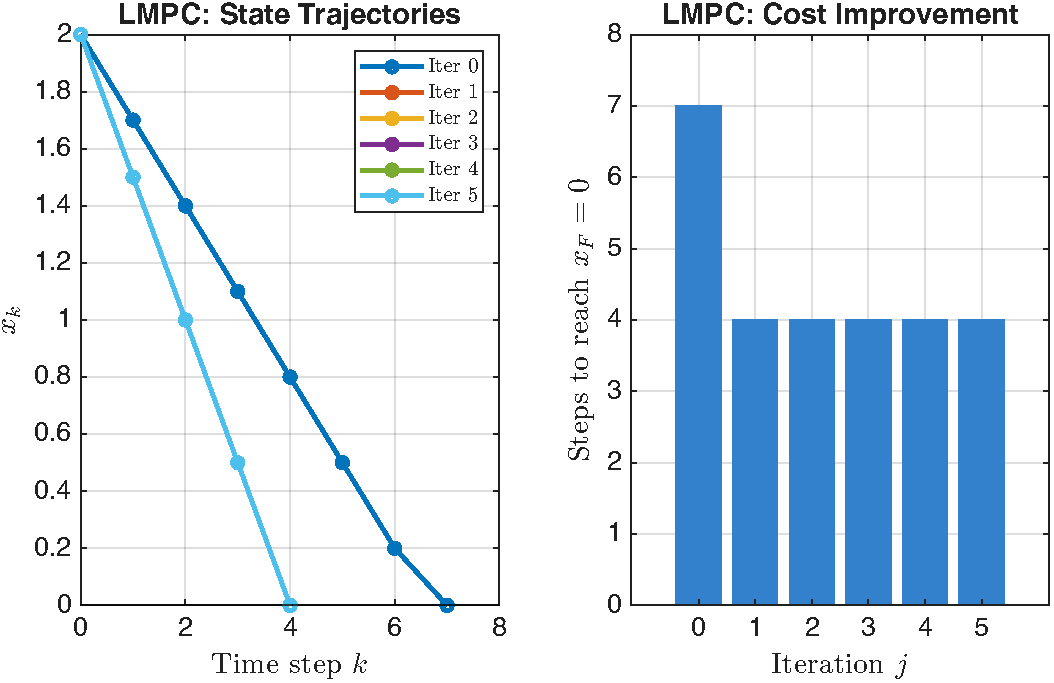
\includegraphics[width=0.92\textwidth]{Figures/fig_lmpc_iterations.pdf}
	\caption{LMPC for the scalar minimum-time problem ($x_{k+1} = x_k + u_k$, $|u_k| \le 0.5$, $x_0 = 2$). Left: state trajectories for iterations~0--5. Iteration~0 (conservative, $u = -0.3$) takes 7~steps. Iterations~1--5 converge to the optimal trajectory using $u = -0.5$ at every step, reaching the origin in~4~steps. Right: the cost (number of steps) decreases monotonically, converging to the theoretical minimum of~4.}
	\label{fig:lmpc_iterations}
\end{figure}


%% ============================================================
%%  WORKED EXAMPLE 2: NN-MPC AUTONOMOUS RACING
%% ============================================================

\subsection{Worked Example: Autonomous Racing with NN-MPC}
\label{sec:nnmpc_racing}

The scalar example above illustrates the LMPC mechanism on a minimal system. We now apply the same principles---safe set expansion, cost-to-go approximation, and iterative improvement---to a realistic nonlinear control problem: \emph{time-optimal autonomous racing} with a dynamic bicycle model and Pacejka tyre forces.

The key departure from the standard LMPC formulation is that the cost-to-go $Q^j$ and the terminal constraint $x_N \in \text{conv}(\mathcal{SS}^j)$ are both approximated by neural networks. This avoids the combinatorial nearest-neighbour search over a growing safe set and provides smooth, differentiable approximations that scale to high-dimensional state spaces.

\subsubsection{Vehicle Model}

The vehicle is modelled as a rear-wheel-drive dynamic bicycle with six states and two inputs:
\begin{equation}\label{eq:racing_state}
	\mathbf{x} = \begin{bmatrix} X \\ Y \\ \varphi \\ v_x \\ v_y \\ r \end{bmatrix}, \qquad
	\mathbf{u} = \begin{bmatrix} \delta \\ D \end{bmatrix},
\end{equation}
where $(X, Y)$ is the position in the global frame, $\varphi$ is the heading angle, $v_x$ and $v_y$ are the longitudinal and lateral velocities in the body frame, $r$ is the yaw rate, $\delta$ is the front steering angle, and $D \in [-1, 1]$ is the normalised throttle/brake command.

The continuous-time dynamics are:
\begin{equation}\label{eq:racing_dynamics}
	\begin{aligned}
		\dot X &= v_x \cos\varphi - v_y \sin\varphi, \\
		\dot Y &= v_x \sin\varphi + v_y \cos\varphi, \\
		\dot\varphi &= r, \\
		\dot v_x &= \tfrac{1}{m}\bigl[F_{rx} - F_{fy}\sin\delta + m\,v_y\,r - F_{\mathrm{drag}}\bigr], \\
		\dot v_y &= \tfrac{1}{m}\bigl[F_{ry} + F_{fy}\cos\delta - m\,v_x\,r\bigr], \\
		\dot r &= \tfrac{1}{I_z}\bigl[F_{fy}\,l_f\cos\delta - F_{ry}\,l_r\bigr].
	\end{aligned}
\end{equation}
Here $m$ is the vehicle mass, $I_z$ the yaw moment of inertia, and $l_f$, $l_r$ the distances from the centre of gravity to the front and rear axles respectively.

\paragraph{Tyre forces.} The lateral tyre forces follow the \emph{Pacejka Magic Formula}~\cite{pacejka2012}. The front and rear slip angles are
\begin{equation}\label{eq:slip_angles}
	\alpha_f = -\arctan\!\frac{v_y + r\,l_f}{v_x} + \delta, \qquad
	\alpha_r = -\arctan\!\frac{v_y - r\,l_r}{v_x},
\end{equation}
and the corresponding lateral forces are
\begin{equation}\label{eq:pacejka}
	F_{fy} = D_f \sin\!\bigl(C_f \arctan(B_f\,\alpha_f)\bigr), \qquad
	F_{ry} = D_r \sin\!\bigl(C_r \arctan(B_r\,\alpha_r)\bigr).
\end{equation}
The longitudinal driving force and drag are modelled as
\begin{equation}\label{eq:drive_drag}
	F_{rx} = C_{m1}\,D - C_{m2}\,D\,v_x, \qquad
	F_{\mathrm{drag}} = C_{r0} + C_{r2}\,v_x^2,
\end{equation}
where $C_{m1}$, $C_{m2}$ capture the motor torque curve and $C_{r0}$, $C_{r2}$ account for rolling resistance and aerodynamic drag. The parameters used in the simulation are listed in Table~\ref{tab:racing_params}.

\begin{table}[ht]
	\centering
	\caption{Vehicle parameters for the racing example.}
	\label{tab:racing_params}
	\begin{tabular}{llrl}
		\toprule
		\textbf{Parameter} & \textbf{Symbol} & \textbf{Value} & \textbf{Unit} \\
		\midrule
		Mass & $m$ & 800 & kg \\
		Yaw inertia & $I_z$ & 1200 & $\text{kg}\cdot\text{m}^2$ \\
		Front axle distance & $l_f$ & 1.2 & m \\
		Rear axle distance & $l_r$ & 1.3 & m \\
		Pacejka front & $B_f,\, C_f,\, D_f$ & $10,\; 1.3,\; 5000$ & $-,\; -,\; \text{N}$ \\
		Pacejka rear & $B_r,\, C_r,\, D_r$ & $11,\; 1.3,\; 7000$ & $-,\; -,\; \text{N}$ \\
		Motor model & $C_{m1},\, C_{m2}$ & $5000,\; 100$ & N, N$\cdot$s/m \\
		Drag model & $C_{r0},\, C_{r2}$ & $50,\; 0.3$ & N, N$\cdot$s$^2$/m$^2$ \\
		Max steering & $\delta_{\max}$ & 0.45 & rad \\
		Throttle range & $D$ & $[-1,\; 1]$ & -- \\
		Speed bounds & $v_x$ & $[0.5,\; 20]$ & m/s \\
		\bottomrule
	\end{tabular}
\end{table}

The dynamics~\eqref{eq:racing_dynamics} are integrated using fourth-order Runge--Kutta with a time step of $\Delta t = 0.05$\,s.


\subsubsection{Track Representation}

The track centreline is constructed as a closed Catmull--Rom spline through 13 waypoints, yielding a circuit of approximately 212\,m. The centreline is parameterised by arc length $s \in [0, L)$, where $L$ is the total track length. At each point, the unit tangent $\mathbf{t}(s)$ and outward normal $\mathbf{n}(s)$ are computed from the spline derivatives, and the local curvature $\kappa(s)$ is obtained from the rate of change of the tangent angle:
\begin{equation}\label{eq:curvature}
	\kappa(s) = \left|\frac{\mathrm{d}\varphi_{\mathrm{tan}}}{\mathrm{d}s}\right|.
\end{equation}
The track boundaries lie at distance $\pm w$ from the centreline along the normal, where $w = 5$\,m is the track half-width.


\subsubsection{Iterative Learning Architecture}
\label{sec:racing_architecture}

The algorithm follows the LMPC paradigm of Section~\ref{sec:lmpc}: iterate between driving and learning, with each lap producing data that improves the next. Two neural networks replace the explicit safe set lookup and convex-hull terminal constraint of the standard LMPC:

\begin{enumerate}
	\item A \textbf{speed map} $v_\theta(s)$ that predicts the target speed at each track position~$s$, replacing the safe-set--based speed targets.
	\item A \textbf{value function} $V_\phi(\mathbf{x})$ that approximates the cost-to-go from any state, replacing the convex-combination terminal cost $Q^j(x_N)$.
\end{enumerate}

\begin{notebox}{Connection to LMPC}
	The speed map encodes the same information as the safe set $\mathcal{SS}^j$: the maximum speed at which the car has been observed to drive safely at each track position. The boost factor $\beta_j$ serves the same purpose as the safe set expansion---it pushes the controller to explore beyond the proven envelope while the curvature cap ensures physical feasibility.
\end{notebox}


\subsubsection{Iteration~0: Data Collection via Pure Pursuit}

The first lap uses a \emph{pure pursuit} controller at a conservative speed $v_{\mathrm{PP}} = 5$\,m/s to complete one full circuit safely. The pure pursuit law computes a lookahead point on the centreline at distance
\begin{equation}\label{eq:lookahead}
	d_{\mathrm{look}} = \max(4\,\text{m},\; 0.9\,v_x)
\end{equation}
ahead of the current arc-length position, then steers towards it. Figure~\ref{fig:nnmpc_pure_pursuit} illustrates the geometry.

\begin{figure}[ht]
	\centering
	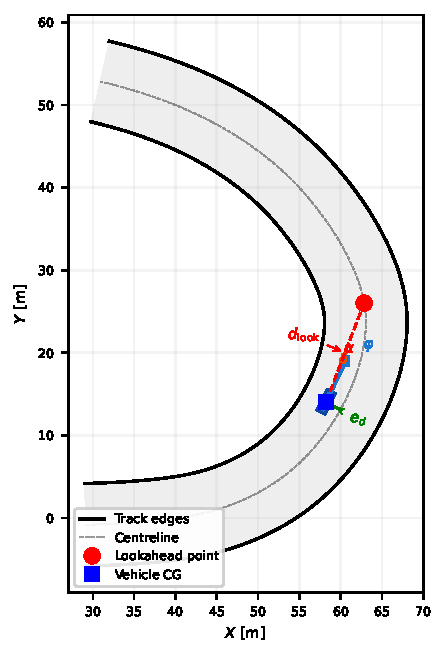
\includegraphics[width=0.65\textwidth]{Figures/fig_nnmpc_pure_pursuit.pdf}
	\caption{Pure pursuit steering geometry. The controller places a lookahead point on the centreline at distance $d_{\mathrm{look}}$ ahead of the vehicle and computes the steering angle $\delta$ from the angle $\alpha$ to that point. If the vehicle drifts off-centre (lateral error $e_d > 0$), the angle $\alpha$ increases and the resulting steering correction pulls the vehicle back towards the centreline.}
	\label{fig:nnmpc_pure_pursuit}
\end{figure}

Let $\alpha$ denote the angle between the vehicle heading and the direction to the lookahead point, and let $d$ be the Euclidean distance to it. The required curvature to intercept the lookahead point is $\gamma = 2\sin\alpha / d$, and the steering angle follows from the bicycle kinematic relation:
\begin{equation}\label{eq:pp_steering}
	\delta = \arctan(\gamma \cdot L_{\mathrm{wb}}), \qquad |\delta| \le \delta_{\max},
\end{equation}
where $L_{\mathrm{wb}} = l_f + l_r$ is the wheelbase. The throttle command is a proportional controller:
\begin{equation}\label{eq:pp_throttle}
	D = \text{clip}\bigl(0.8\,(v_{\mathrm{target}} - v_x),\; -1,\; 1\bigr).
\end{equation}

This controller is inherently self-correcting: if the vehicle drifts off-centre, the angle $\alpha$ to the lookahead point increases, producing a larger steering correction. At the end of iteration~0, the full trajectory $\{(\mathbf{x}_k^{(0)}, \mathbf{u}_k^{(0)}, s_k^{(0)})\}_{k=0}^{T_0}$ is stored.


\subsubsection{NN Speed Map: Learning How Fast to Drive}
\label{sec:racing_speed_map}

After each completed lap, a neural network learns the optimal speed at each track position. The training data is constructed in four stages, illustrated in Figure~\ref{fig:nnmpc_speed_pipeline}.

\begin{figure}[ht]
	\centering
	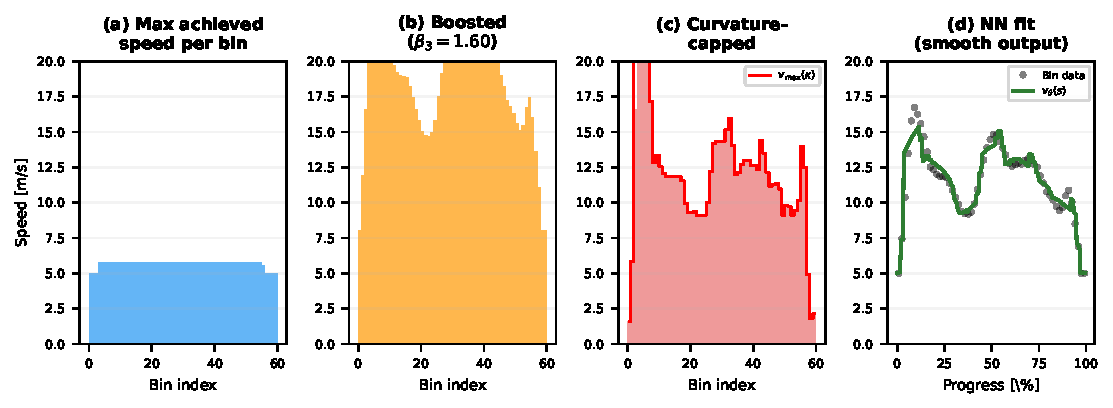
\includegraphics[width=0.95\textwidth]{Figures/fig_nnmpc_speed_pipeline.pdf}
	\caption{NN speed map training pipeline. (a)~The track is divided into $N_{\mathrm{bin}} = 60$ bins and the maximum achieved speed in each bin forms the safe set. (b)~A boost factor $\beta_j$ pushes targets beyond proven speeds. (c)~Curvature-based speed limits cap bins at tight corners. (d)~An \texttt{MLPRegressor} fits a smooth speed profile to the binned data.}
	\label{fig:nnmpc_speed_pipeline}
\end{figure}

\paragraph{Stage~1: Safe set of speeds.} The track is divided into $N_{\mathrm{bin}} = 60$ equal-length bins. For each bin $b$, the maximum longitudinal speed achieved at any point in that bin across all completed iterations is recorded:
\begin{equation}\label{eq:bin_speed}
	\bar{v}_b^{(j)} = \max_{i \le j}\;\max_{k:\, s_k^{(i)} \in \text{bin}\,b}\; v_{x,k}^{(i)}.
\end{equation}
This is the speed-map analogue of the safe set $\mathcal{SS}^j$: the car has been observed driving safely at speed $\bar{v}_b^{(j)}$ in bin $b$.

\paragraph{Stage~2: Iteration-based boost.} To push beyond proven speeds (analogous to safe set expansion), the bin speeds are multiplied by a boost factor that grows with the iteration count:
\begin{equation}\label{eq:boost}
	\tilde{v}_b^{(j)} = \bar{v}_b^{(j)} \cdot \beta_j, \qquad
	\beta_j = \min\!\bigl(1 + 0.15\,(j+1),\; 3.0\bigr).
\end{equation}
This is a controlled extrapolation: at iteration~0, $\beta_0 = 1.15$ (15\% above proven speed); by iteration~7, $\beta_7 = 2.20$. The cap at $3.0$ prevents unbounded growth.

\paragraph{Stage~3: Curvature speed limit.} The boosted targets are capped by the maximum speed that the tyres can sustain through each corner. The steady-state cornering condition requires the lateral acceleration to remain below a threshold $a_{\mathrm{lat,max}}$:
\begin{equation}\label{eq:curv_limit}
	v_{\max}(s) = \sqrt{\frac{a_{\mathrm{lat,max}}}{\kappa(s)}},
\end{equation}
where $\kappa(s)$ is the local curvature. With $a_{\mathrm{lat,max}} = 6\,\text{m/s}^2$, a corner with $\kappa = 0.1\,\text{rad/m}$ limits speed to $\sqrt{60} \approx 7.7$\,m/s. The curvature is smoothed over a window of $\pm 3$ bins to account for the vehicle's spatial extent. Figure~\ref{fig:nnmpc_curvature_speed} shows the curvature profile and the resulting speed limits.

\begin{figure}[ht]
	\centering
	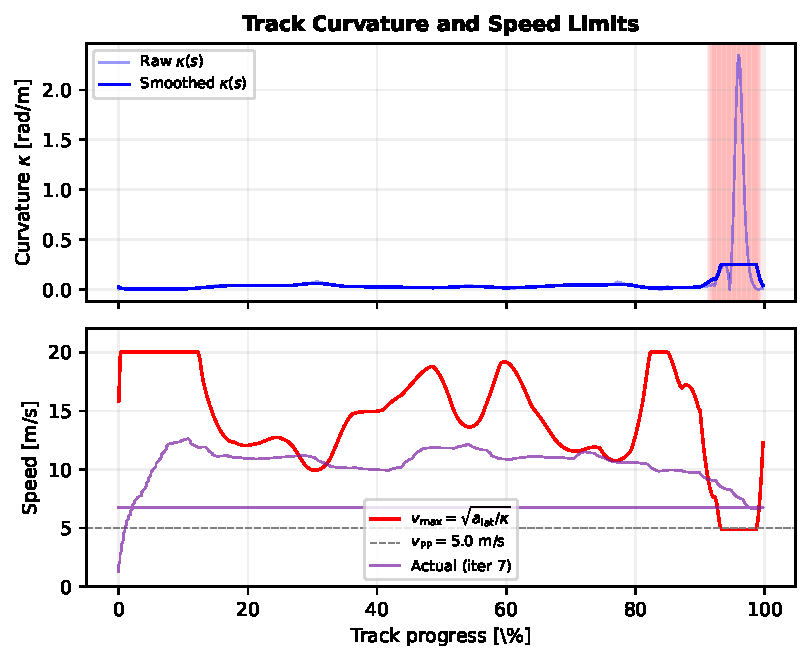
\includegraphics[width=0.7\textwidth]{Figures/fig_nnmpc_curvature_speed.pdf}
	\caption{Top: track curvature $\kappa(s)$ (raw and smoothed). High-curvature zones are shaded. Bottom: curvature-based speed limit $v_{\max} = \sqrt{a_{\mathrm{lat,max}}/\kappa}$ (red), conservative baseline speed $v_{\mathrm{PP}} = 5$\,m/s (dashed grey), and actual speed from the final iteration (purple). The car learns to approach the curvature limit on straights whilst respecting it through corners.}
	\label{fig:nnmpc_curvature_speed}
\end{figure}

The final target speed for each bin combines all three stages:
\begin{equation}\label{eq:target_speed}
	v_{\mathrm{target},b}^{(j)} = \text{clip}\!\left(\min\!\bigl(\tilde{v}_b^{(j)},\; v_{\max,b}\bigr),\; v_{\mathrm{PP}},\; v_{x,\max}\right),
\end{equation}
followed by a 5-bin moving-average smooth to remove discontinuities.

\paragraph{Stage~4: Neural network fit.} An \texttt{MLPRegressor} with two hidden layers of 64 and 32 neurons (\texttt{ReLU} activation) is trained on the binned data. The input features are
\begin{equation}\label{eq:speed_features}
	\mathbf{z}(s) = \left[\frac{s}{L},\;\; \kappa(s),\;\; \sin\!\frac{2\pi s}{L},\;\; \cos\!\frac{2\pi s}{L}\right],
\end{equation}
and the output is the target speed. The Fourier features $\sin(2\pi s/L)$ and $\cos(2\pi s/L)$ encode the periodic (closed-loop) nature of the track, allowing the network to generalise across the start/finish line. The curvature input $\kappa$ provides a direct geometric signal. Five training samples per bin (at uniformly spaced offsets within each bin) give 300 training points in total.


\subsubsection{NN Value Function: Learning the Cost-to-Go}

A second neural network $V_\phi(\mathbf{x})$ approximates the cost-to-go from any state, replacing the convex-combination terminal cost of the standard LMPC~\eqref{eq:lmpc_opt}. With stage cost $\ell = 1$ (minimum-time objective), the cost-to-go from state $\mathbf{x}_k^{(i)}$ is
\begin{equation}\label{eq:vf_target}
	Q^j(\mathbf{x}_k^{(i)}) = T_i - k,
\end{equation}
where $T_i$ is the total number of steps in iteration $i$. Training data from all completed laps is accumulated and the network is retrained after each iteration. The input features are:
\begin{equation}\label{eq:vf_features}
	\mathbf{z}_V(\mathbf{x}) = \left[\frac{X}{50},\;\; \frac{Y}{50},\;\; \cos\varphi,\;\; \sin\varphi,\;\; \frac{v_x}{v_{x,\max}}\right].
\end{equation}
The position is normalised by 50\,m to match the track scale. The heading is encoded as $(\cos\varphi, \sin\varphi)$ to avoid the discontinuity at $\varphi = \pm\pi$. The network architecture is the same as the speed map (two hidden layers of 64 and 32 neurons).


\subsubsection{MPC Controller}
\label{sec:racing_mpc}

At each control step (every $2 \times \Delta t = 0.1$\,s), the controller computes a target speed through four sub-steps:

\paragraph{Step~1: Query the speed map.} The current arc-length position $s$ is obtained by projecting the vehicle position $(X, Y)$ onto the centreline using a KD-tree nearest-neighbour search. The NN speed map returns the target speed:
\begin{equation}\label{eq:mpc_step1}
	v_{\mathrm{target}} = v_\theta(s).
\end{equation}

\paragraph{Step~2: Lookahead braking.} The controller checks the speed map at positions $\Delta t_{\mathrm{look}} \in \{0.5, 1.0, 1.5\}$\,s ahead of the current position. If the target speed is lower ahead (a corner is approaching), the current target is reduced to allow time for deceleration:
\begin{equation}\label{eq:mpc_step2}
	v_{\mathrm{target}} \leftarrow \min\!\Bigl(v_{\mathrm{target}},\;\;
	v_\theta\bigl(s + v_x \cdot \Delta t_{\mathrm{look}}\bigr) + 1.5 \cdot \Delta t_{\mathrm{look}}\Bigr).
\end{equation}
The term $+1.5 \cdot \Delta t_{\mathrm{look}}$ is a deceleration budget: the car may maintain a higher speed now if the corner is still far away. Figure~\ref{fig:nnmpc_lookahead} illustrates this mechanism.

\begin{figure}[ht]
	\centering
	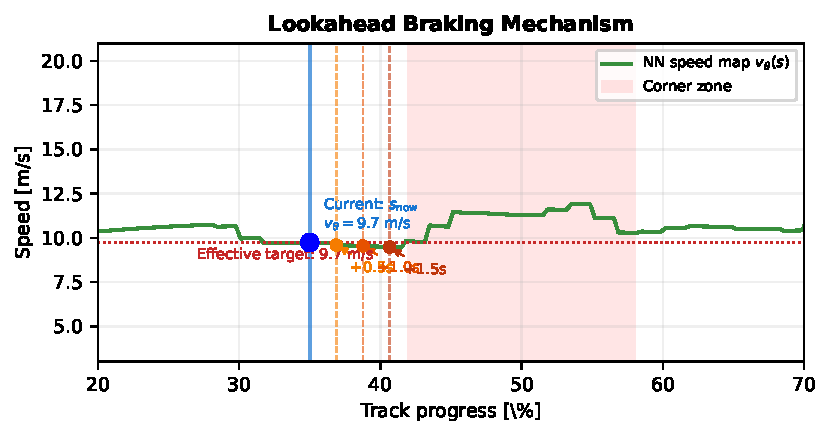
\includegraphics[width=0.7\textwidth]{Figures/fig_nnmpc_lookahead_braking.pdf}
	\caption{Lookahead braking. The controller queries the NN speed map at positions 0.5, 1.0, and 1.5\,s ahead. The corner zone (shaded) has a lower target speed. The effective target at the current position is reduced below the local value $v_\theta(s_{\mathrm{now}})$ to allow proactive deceleration before the corner.}
	\label{fig:nnmpc_lookahead}
\end{figure}

\paragraph{Step~3: Value function adjustment.} The controller evaluates the value function at two hypothetical states: $\mathbf{x}_{\mathrm{fast}}$ with $v_x = v_{\mathrm{target}}$ and $\mathbf{x}_{\mathrm{slow}}$ with $v_x = 0.8\,v_{\mathrm{target}}$. If $V_\phi(\mathbf{x}_{\mathrm{fast}}) < V_\phi(\mathbf{x}_{\mathrm{slow}})$, the faster state leads to lower remaining cost, and the target speed is increased by~5\%:
\begin{equation}\label{eq:mpc_step3}
	v_{\mathrm{target}} \leftarrow
	\begin{cases}
		\min(1.05 \cdot v_{\mathrm{target}},\; v_{x,\max}) & \text{if } V_\phi(\mathbf{x}_{\mathrm{fast}}) < V_\phi(\mathbf{x}_{\mathrm{slow}}), \\
		v_{\mathrm{target}} & \text{otherwise.}
	\end{cases}
\end{equation}

\paragraph{Step~4: Execute.} The computed target speed is passed to the pure pursuit controller~\eqref{eq:pp_steering}--\eqref{eq:pp_throttle}, which returns the steering angle $\delta$ and throttle command~$D$.

Algorithm~\ref{alg:nnmpc} summarises the complete NN-MPC procedure, combining the outer iterative learning loop with the inner control loop.

\begin{algorithm}[ht]
\caption{NN-MPC Iterative Learning for Autonomous Racing}
\label{alg:nnmpc}
\begin{algorithmic}[1]
\Require Track centreline $\{(X(s), Y(s))\}$, vehicle model $f$, number of iterations $J$
\Ensure Trajectories $\{\mathbf{x}^{(j)}, \mathbf{u}^{(j)}\}_{j=0}^{J-1}$ with non-increasing lap times

\Statex \textbf{--- Iteration 0: Data Collection ---}
\State Run one lap with pure pursuit at $v_{\mathrm{PP}} = 5$\,m/s using~\eqref{eq:pp_steering}--\eqref{eq:pp_throttle}
\State Store trajectory $\{(\mathbf{x}_k^{(0)}, \mathbf{u}_k^{(0)}, s_k^{(0)})\}_{k=0}^{T_0}$
\State Initialise safe set $\mathcal{SS}^0$ and cost-to-go $Q^0$

\Statex \textbf{--- Iterations $j = 1, \ldots, J-1$: NN-MPC ---}
\For{$j = 1$ \textbf{to} $J-1$}
    \Statex \quad \textit{Train neural networks:}
    \State Build binned speed targets $\bar{v}_b^{(j)}$ from $\mathcal{SS}^{j-1}$  \hfill \Comment{Eq.~\eqref{eq:bin_speed}}
    \State Apply boost $\hat{v}_b^{(j)} = \bar{v}_b^{(j)} \cdot \beta_j$, cap by curvature $v_{\max}(s)$ \hfill \Comment{Eqs.~\eqref{eq:boost},~\eqref{eq:curv_limit}}
    \State Train speed map $v_\theta(s)$ on binned data \hfill \Comment{MLPRegressor}
    \State Train value function $V_\phi(\mathbf{x})$ on cost-to-go data \hfill \Comment{MLPRegressor}

    \Statex \quad \textit{Run lap with learned controller:}
    \For{each control step ($k = 0, 1, 2, \ldots$) until lap complete}
        \State $v_{\mathrm{target}} \gets v_\theta(s_k)$ \hfill \Comment{Step 1: query speed map}
        \State $v_{\mathrm{target}} \gets \min\!\bigl(v_{\mathrm{target}},\; v_\theta(s_k + v_x \Delta t_{\mathrm{look}}) + 1.5\,\Delta t_{\mathrm{look}}\bigr)$ \hfill \Comment{Step 2: lookahead braking}
        \If{$V_\phi(\mathbf{x}_{\mathrm{fast}}) < V_\phi(\mathbf{x}_{\mathrm{slow}})$} \hfill \Comment{Step 3: value function check}
            \State $v_{\mathrm{target}} \gets \min(1.05 \cdot v_{\mathrm{target}},\; v_{x,\max})$
        \EndIf
        \State Compute $\delta, D$ via pure pursuit~\eqref{eq:pp_steering}--\eqref{eq:pp_throttle} at $v_{\mathrm{target}}$ \hfill \Comment{Step 4: execute}
        \State Apply $(\delta, D)$ to vehicle; integrate dynamics~\eqref{eq:racing_dynamics}
    \EndFor
    \State Store trajectory; update $\mathcal{SS}^j$ and $Q^j$
\EndFor
\end{algorithmic}
\end{algorithm}


\subsubsection{Track-Keeping Mechanisms}

The controller uses no explicit wall or track-boundary constraints. Instead, four complementary mechanisms keep the vehicle within the track:
\begin{enumerate}
	\item \emph{Pure pursuit geometry.} The steering law~\eqref{eq:pp_steering} always aims at a point on the centreline. If the vehicle drifts off-centre, the angle $\alpha$ to the lookahead point increases, producing a larger corrective steering input. This makes the controller inherently self-stabilising.

	\item \emph{Curvature speed limits.} The bound~\eqref{eq:curv_limit} prevents the speed map from requesting speeds that exceed the lateral grip of the tyres. This is the primary mechanism for corner safety.

	\item \emph{Lookahead braking.} The predictive check~\eqref{eq:mpc_step2} ensures the vehicle begins decelerating before reaching a tight corner, rather than reacting only after entering it.

	\item \emph{Off-track abort.} If the lateral deviation from the centreline exceeds $3w$ (15\,m), the lap is aborted. In practice, mechanisms~1--3 keep the deviation below approximately 1.1\,m, well within the 5\,m half-width.
\end{enumerate}


\subsubsection{Safe Set Expansion Over Iterations}

Figure~\ref{fig:nnmpc_safe_set} shows how the safe set grows over iterations. After iteration~0, only a narrow band of states near the centreline has been explored (at 5\,m/s). By iteration~7, the safe set contains over 4\,000 state measurements spanning a wide range of speeds and positions. The colour encodes longitudinal speed---the progression from blue (slow) to red (fast) shows that later iterations reach higher speeds on the straights whilst maintaining safe speeds through corners.

\begin{figure}[ht]
	\centering
	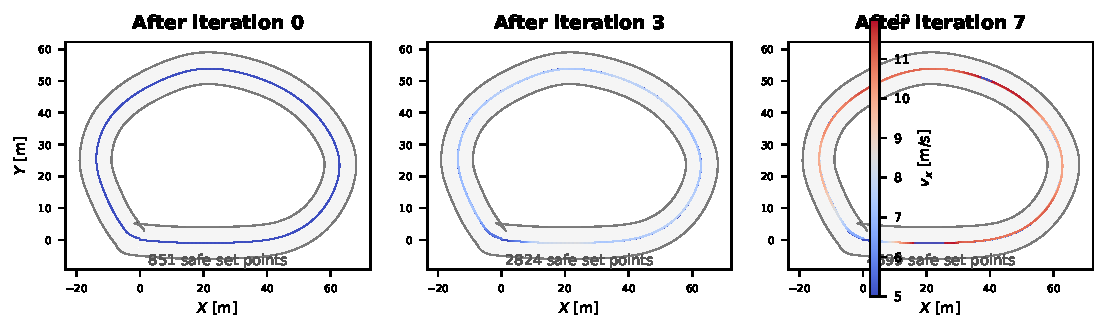
\includegraphics[width=0.95\textwidth]{Figures/fig_nnmpc_safe_set.pdf}
	\caption{Safe set expansion over iterations. Each point is a state visited during a completed lap, coloured by longitudinal speed $v_x$. After iteration~0, only conservative low-speed states are known. By iteration~7, the safe set spans a wide speed range, with higher speeds on straights and lower speeds at corners.}
	\label{fig:nnmpc_safe_set}
\end{figure}


\subsubsection{Simulation Results}

The simulation runs 8~iterations on the custom 13-waypoint track (212\,m). Total computation time is approximately 6\,s on a standard laptop. Figure~\ref{fig:nnmpc_racing_results} presents the results in four panels.

\begin{figure}[ht]
	\centering
	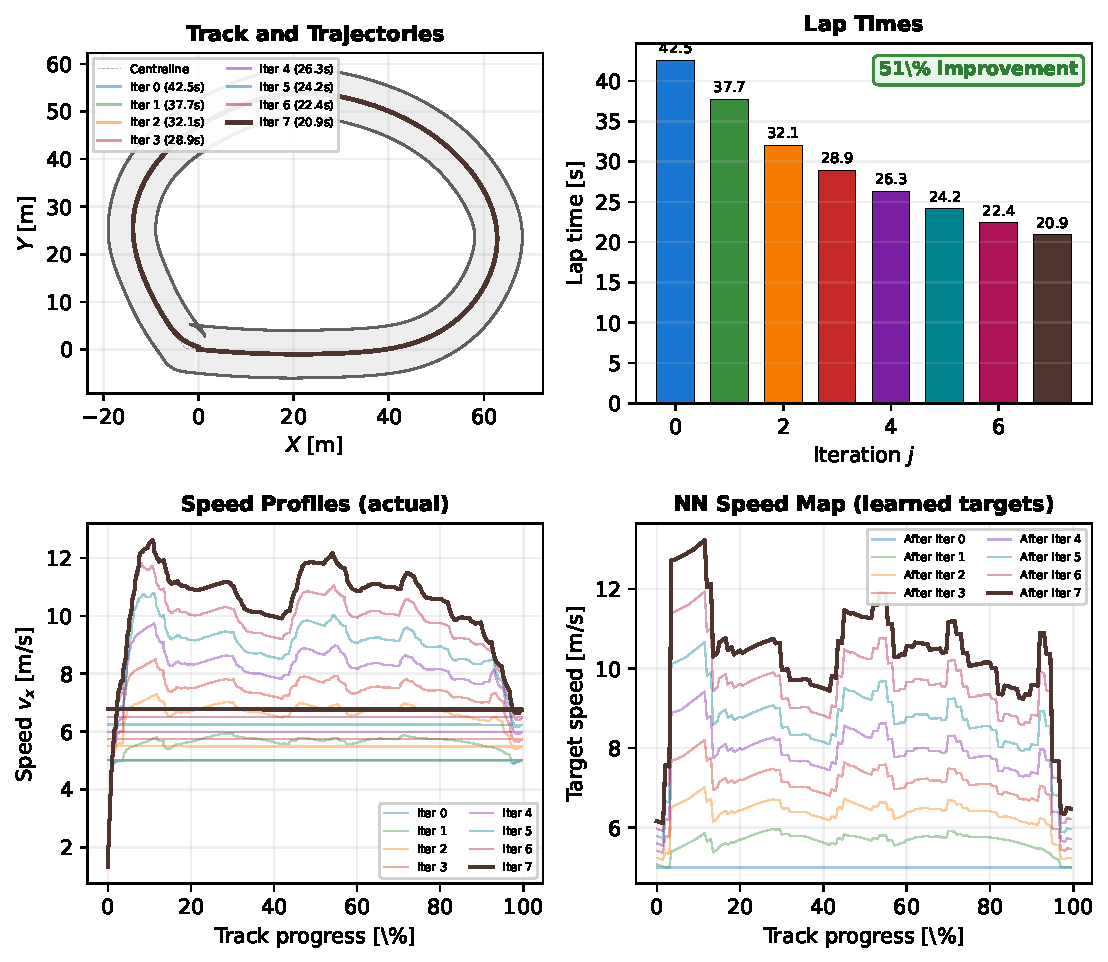
\includegraphics[width=0.95\textwidth]{Figures/fig_nnmpc_racing_results.pdf}
	\caption{NN-MPC autonomous racing results over 8~iterations. Top left: track with overlaid trajectories---later iterations carry higher speed through straights whilst maintaining the racing line through corners. Top right: lap times decrease monotonically from 42.5\,s (pure pursuit at 5\,m/s) to 20.9\,s (NN-MPC at average 10.1\,m/s), a 51\% improvement. Bottom left: actual speed profiles---the car learns to accelerate harder on straights and brake later into corners. Bottom right: NN speed map evolution showing how the learned target speeds increase with each iteration (capped by curvature at corners).}
	\label{fig:nnmpc_racing_results}
\end{figure}

The key observations are:
\begin{itemize}
	\item \emph{Monotone cost decrease.} Lap times decrease from 42.5\,s to 20.9\,s (51\% improvement), consistent with the non-increasing cost property of LMPC (Section~\ref{sec:lmpc_guarantees}).

	\item \emph{Speed profiles.} Iteration~0 drives at a near-constant 5\,m/s. By iteration~7, the car reaches 12.6\,m/s on the straights and brakes to approximately 7\,m/s through tight corners---the curvature speed limit~\eqref{eq:curv_limit} is the binding constraint.

	\item \emph{NN speed map convergence.} The learned speed targets increase rapidly in early iterations and converge as the boost factor saturates and the curvature limits bind. The network produces a smooth, position-dependent speed profile that the pure pursuit controller can track reliably.

	\item \emph{Track safety.} The maximum lateral deviation from the centreline remains below 1.1\,m throughout all 8~iterations. The vehicle never leaves the track.
\end{itemize}

Table~\ref{tab:racing_results} summarises the iteration-by-iteration improvement.

\begin{table}[ht]
	\centering
	\caption{NN-MPC racing results: lap times and average speeds over 8~iterations on the 212\,m track.}
	\label{tab:racing_results}
	\begin{tabular}{crrrc}
		\toprule
		\textbf{Iteration} & \textbf{Lap time [s]} & \textbf{Avg.\ speed [m/s]} & \textbf{Max $|e_d|$ [m]} & \textbf{Controller} \\
		\midrule
		0 & 42.5 & 5.0 & 0.9 & Pure pursuit \\
		1 & 37.7 & 5.6 & 0.9 & NN-MPC \\
		2 & 32.1 & 6.6 & 1.0 & NN-MPC \\
		3 & 28.9 & 7.3 & 1.1 & NN-MPC \\
		4 & 26.3 & 8.0 & 1.1 & NN-MPC \\
		5 & 24.2 & 8.7 & 1.1 & NN-MPC \\
		6 & 22.4 & 9.4 & 1.1 & NN-MPC \\
		7 & 20.9 & 10.1 & 1.1 & NN-MPC \\
		\bottomrule
	\end{tabular}
\end{table}

\begin{alertbox}{Why not solve a full nonlinear MPC online?}
	A ``proper'' LMPC for this system would solve a nonlinear programme with dynamic bicycle constraints at each time step, using the safe set as the terminal constraint. This is computationally demanding---the Pacejka tyre model is highly nonlinear, the state space is six-dimensional, and the safe set grows with every iteration. The NN-MPC approach demonstrated here is a practical approximation: the two neural networks distil the safe set and cost-to-go information into smooth, cheap-to-evaluate functions, and the pure pursuit + proportional speed controller provides a computationally trivial inner loop. The trade-off is that the controller does not optimise a multi-step prediction horizon at each time step---it relies on the NN speed map to encode the optimal speed schedule implicitly. For teaching purposes, this makes the LMPC concept accessible without requiring a browser-based or desktop nonlinear solver.
\end{alertbox}

\begin{notebox}{Running the simulation}
	The companion Python script \texttt{lmpc\_racing.py} implements this example. It requires \texttt{numpy}, \texttt{scipy}, \texttt{scikit-learn}, and \texttt{matplotlib}. Students can modify the \texttt{USER SETTINGS} section to experiment with: the boost factor $\beta_j$ (\texttt{SPEED\_BOOST}), the curvature limit $a_{\mathrm{lat,max}}$ (\texttt{A\_LAT\_MAX}), the network architecture (\texttt{NN\_SPEED\_LAYERS}), the number of iterations, and the track choice (three tracks are included: a 13-waypoint custom circuit and two tracks from the MPCC benchmark~\cite{liniger2015optimization}).

	\medskip
	\textbf{Code:} \url{https://kucukdemiral.github.io/lmpc_racing.py}\\
	\textbf{Colab notebook:} \url{https://kucukdemiral.github.io/lmpc_racing.ipynb}
\end{notebox}


%% ============================================================
%%  SECTION 6: NEURAL NETWORK MODELS IN MPC
%% ============================================================
\section{Neural Network Models in MPC}
\label{sec:nnmpc}

A feedforward neural network can approximate any continuous function to arbitrary accuracy, given enough neurons. This makes it a natural candidate for learning unknown dynamics $x_{k+1} = f_\theta(x_k, u_k)$, where $\theta$ denotes the network weights.

Training is standard: given trajectory data $\{(x_k, u_k, x_{k+1})\}$, minimise the prediction error:
\[
\min_\theta \sum_{k} \|x_{k+1} - f_\theta(x_k, u_k)\|^2
\]
using gradient descent (backpropagation). After training, $f_\theta$ is embedded in the MPC as the prediction model.

\begin{alertbox}{Convexity Structure of Learning-Based MPC}
	A key practical distinction among the methods in this chapter is whether the resulting online optimisation is a convex QP or a non-convex NLP:
	\begin{itemize}[noitemsep]
		\item \emph{Koopman MPC} is a \emph{linear MPC} in the lifted coordinates. The dynamics $z_{k+1} = A_K z_k + B_K u_k$ are linear, the cost is quadratic, and the constraints are linear in the lifted state. The nonlinear lifting $\Psi(x)$ is evaluated only \emph{once} at the measured state to form the initial condition $z_0 = \Psi(x(t))$---a fixed parameter, not a decision variable. The result is a standard QP.
		\item \emph{DeePC} is also a \emph{linear MPC}: the Hankel-matrix constraint is linear in the decision variable $g$, the cost is quadratic, and the $\|\sigma_y\|_2^2$ slack penalty is quadratic. The $\ell_1$ regularisation $\|g\|_1$ is handled by introducing auxiliary variables and linear constraints, so YALMIP reformulates the entire problem as a QP solvable by \texttt{quadprog}.
		\item \emph{GP-MPC} is an NLP. The GP mean $\mu_g(x_k, u_k)$ and variance $\sigma_g^2(x_k, u_k)$ are nonlinear functions of the predicted states, which are decision variables. A common approximation is to evaluate the GP at the \emph{current nominal trajectory} (not the optimised one) and solve a single QP---this is a successive linearisation, not an exact solution.
		\item \emph{NN-MPC} is also an NLP, and typically the most difficult one: neural network activation functions (ReLU, tanh) create a non-smooth, multi-modal landscape with many local minima. A general NLP solver (e.g.\ IPOPT via CasADi) is required.
	\end{itemize}
	In short: Koopman MPC and DeePC preserve the QP structure of standard linear MPC. GP-MPC and NN-MPC do not.
\end{alertbox}

Practical workarounds include:
\begin{itemize}
	\item \emph{Linearise the NN} at each time step (similar to the Real-Time Iteration scheme in Chapter~10), producing a time-varying QP.
	\item \emph{Use the NN for warm-starting}: compute an initial guess with the NN, then refine with a simpler model-based MPC.
	\item \emph{Approximate the MPC policy}: train a NN to clone the MPC controller's input--output map $\pi_\theta(x) \approx u_0^*(x)$, eliminating the online optimisation entirely.
\end{itemize}

The following code demonstrates learning a scalar dynamics model with a simple NN and comparing its predictions to the GP from Section~\ref{sec:gpmpc_example}.

\begin{lstlisting}[language=Matlab, caption={NN dynamics learning for the scalar drag system.}]
% 1. Training Data (same system as GP-MPC example)
rng(0);
T_data = 50;
x_nn = zeros(T_data+1, 1);
u_nn = 2*rand(T_data, 1) - 1;
for k = 1:T_data
    x_nn(k+1) = x_nn(k) + u_nn(k) - 0.2*x_nn(k)^3;
end
X_in  = [x_nn(1:T_data), u_nn];   % inputs: [x_k, u_k]
Y_out = x_nn(2:T_data+1);          % targets: x_{k+1}

% 2. Train a Simple NN (1 hidden layer, 20 neurons)
net = fitnet(20, 'trainlm');
net.trainParam.showWindow = false;
net = train(net, X_in', Y_out');

% 3. Compare Predictions (u = 0)
x_test = linspace(-3, 3, 100);
y_true = x_test + 0 - 0.2*x_test.^3;
y_nn   = net([x_test; zeros(1,100)]);

figure; plot(x_test, y_true, 'r-', 'LineWidth', 2); hold on;
plot(x_test, y_nn, 'b--', 'LineWidth', 2);
xlabel('x_k'); ylabel('x_{k+1}');
legend('True dynamics', 'NN prediction');
title('Neural Network One-Step Prediction (u = 0)'); grid on;
\end{lstlisting}

Figure~\ref{fig:nn_prediction} shows the NN one-step prediction. The NN (blue dashed) captures the nonlinear dynamics well within the training range, though unlike the GP it provides no confidence measure.

\begin{figure}[ht]
	\centering
	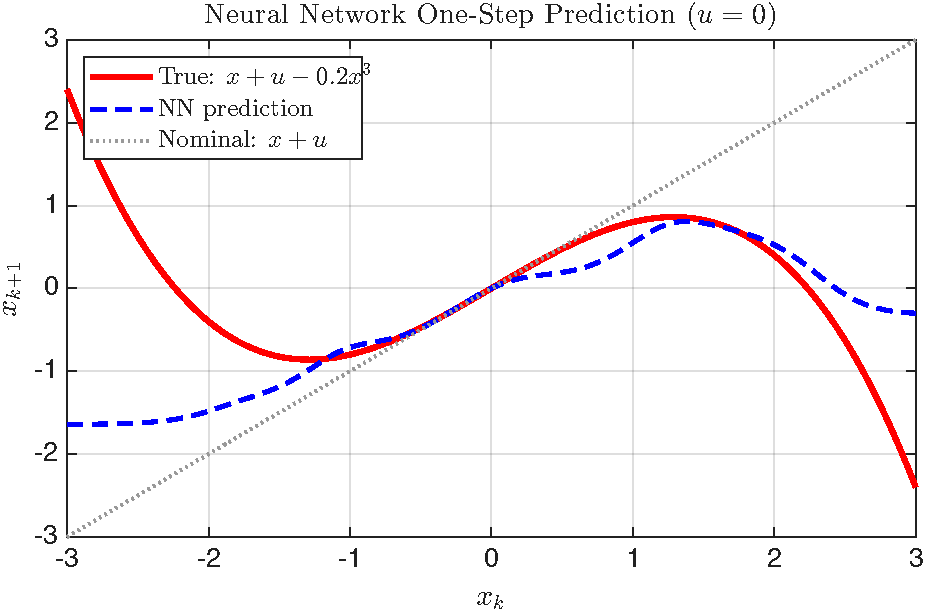
\includegraphics[width=0.82\textwidth]{Figures/fig_nn_prediction.pdf}
	\caption{Neural network one-step prediction for the scalar system $x_{k+1} = x_k + u_k - 0.2\,x_k^3$ (with $u = 0$). A single-hidden-layer NN with 20 neurons (blue dashed) matches the true dynamics (red solid) within the training range $|x| \lesssim 3$. The nominal model $x_{k+1} = x_k$ (grey dotted) ignores the cubic drag entirely. Unlike the GP (Figure~\ref{fig:gp_residual}), the NN provides a point prediction with no uncertainty quantification.}
	\label{fig:nn_prediction}
\end{figure}


%% ============================================================
%%  SECTION 7: REINFORCEMENT LEARNING AND MPC
%% ============================================================
\section{Reinforcement Learning and MPC --- Connections}
\label{sec:rl_mpc}

Reinforcement learning (RL) and MPC solve closely related problems: both seek a policy $\pi(x)$ that minimises cumulative cost (or maximises cumulative reward) over time. The difference is in what is assumed known.

\begin{summarybox}{MPC $\leftrightarrow$ RL Correspondences}
	\begin{center}
		\begin{tabular}{l l}
			\toprule
			\emph{MPC concept} & \emph{RL concept} \\
			\midrule
			Stage cost $\ell(x_k, u_k)$ & Negative reward $-r(s_k, a_k)$ \\
			Terminal cost $V_f(x_N)$ & Value function $V(s)$ \\
			Model $x_{k+1} = f(x_k, u_k)$ & Transition model $P(s'|s, a)$ \\
			Prediction horizon $N$ & Discount factor $\gamma$ (conceptually) \\
			Receding horizon & Model-based replanning \\
			\bottomrule
		\end{tabular}
	\end{center}
\end{summarybox}

Three productive ways to combine RL and MPC:

\emph{1.\ MPC as a structured policy in RL.} Rather than learning a policy from scratch (a neural network mapping states to actions), use the MPC controller $\pi_\text{MPC}(x) = u_0^*(x)$ as the policy. The MPC structure provides constraint satisfaction and stability by construction---RL then tunes the MPC parameters ($Q$, $R$, $N$, or the model itself) to maximise long-term performance.

\emph{2.\ RL for MPC tuning.} The cost matrices $Q$ and $R$ are typically hand-tuned. RL can automate this: treat $Q$ and $R$ as the ``action'' of an outer-loop agent, evaluate the resulting MPC performance over a simulation episode, and update $Q$ and $R$ via policy gradient or Bayesian optimisation.

\emph{3.\ MPC as a safe exploration policy.} During RL training, the agent must explore, which can lead to constraint violations. By using MPC with conservative constraints as the exploration policy, the system remains safe while the RL agent collects data to improve its value function.

\begin{lstlisting}[language=Matlab, caption={RL-style tuning of MPC weight $R$ on a scalar system.}]
% 1. System
A = 1;  B = 1;  Q = 1;  N = 5;  x0 = 3;  T_ep = 20;
f = @(x, u) A*x + B*u;

% 2. Evaluate one episode with given R
run_episode = @(R_val) eval_mpc(A, B, Q, R_val, N, x0, T_ep);

% 3. Grid Search (simple RL: evaluate cost for each R)
R_grid = logspace(-2, 1, 30);
J_grid = zeros(size(R_grid));
for i = 1:length(R_grid)
    J_grid(i) = run_episode(R_grid(i));
end
[J_best, idx] = min(J_grid);
fprintf('Best R = %.3f, Cost = %.2f\n', R_grid(idx), J_best);

figure; semilogx(R_grid, J_grid, 'b-o', 'LineWidth', 2);
xlabel('R (control weight)'); ylabel('Episode cost J');
title('RL-Style Tuning of MPC Weight R'); grid on;

% --- Helper function ---
function J = eval_mpc(A, B, Q, R, N, x0, T_ep)
    P = dare(A, B, Q, R);
    x = x0; J = 0;
    for t = 1:T_ep
        % Simple unconstrained MPC (LQR) for speed
        K = (R + B'*P*B) \ (B'*P*A);
        u = -K * x;
        J = J + Q*x^2 + R*u^2;
        x = A*x + B*u;
    end
    J = J + x'*P*x;
end
\end{lstlisting}


%% ============================================================
%%  SECTION 8: PRACTICAL GUIDELINES
%% ============================================================
\section{Practical Guidelines and Comparison}
\label{sec:comparison}

The choice of method depends on the application context. The decision flowchart in Figure~\ref{fig:method_flowchart} provides a practical guide, and the following questions summarise the logic.

\begin{figure}[ht]
	\centering
	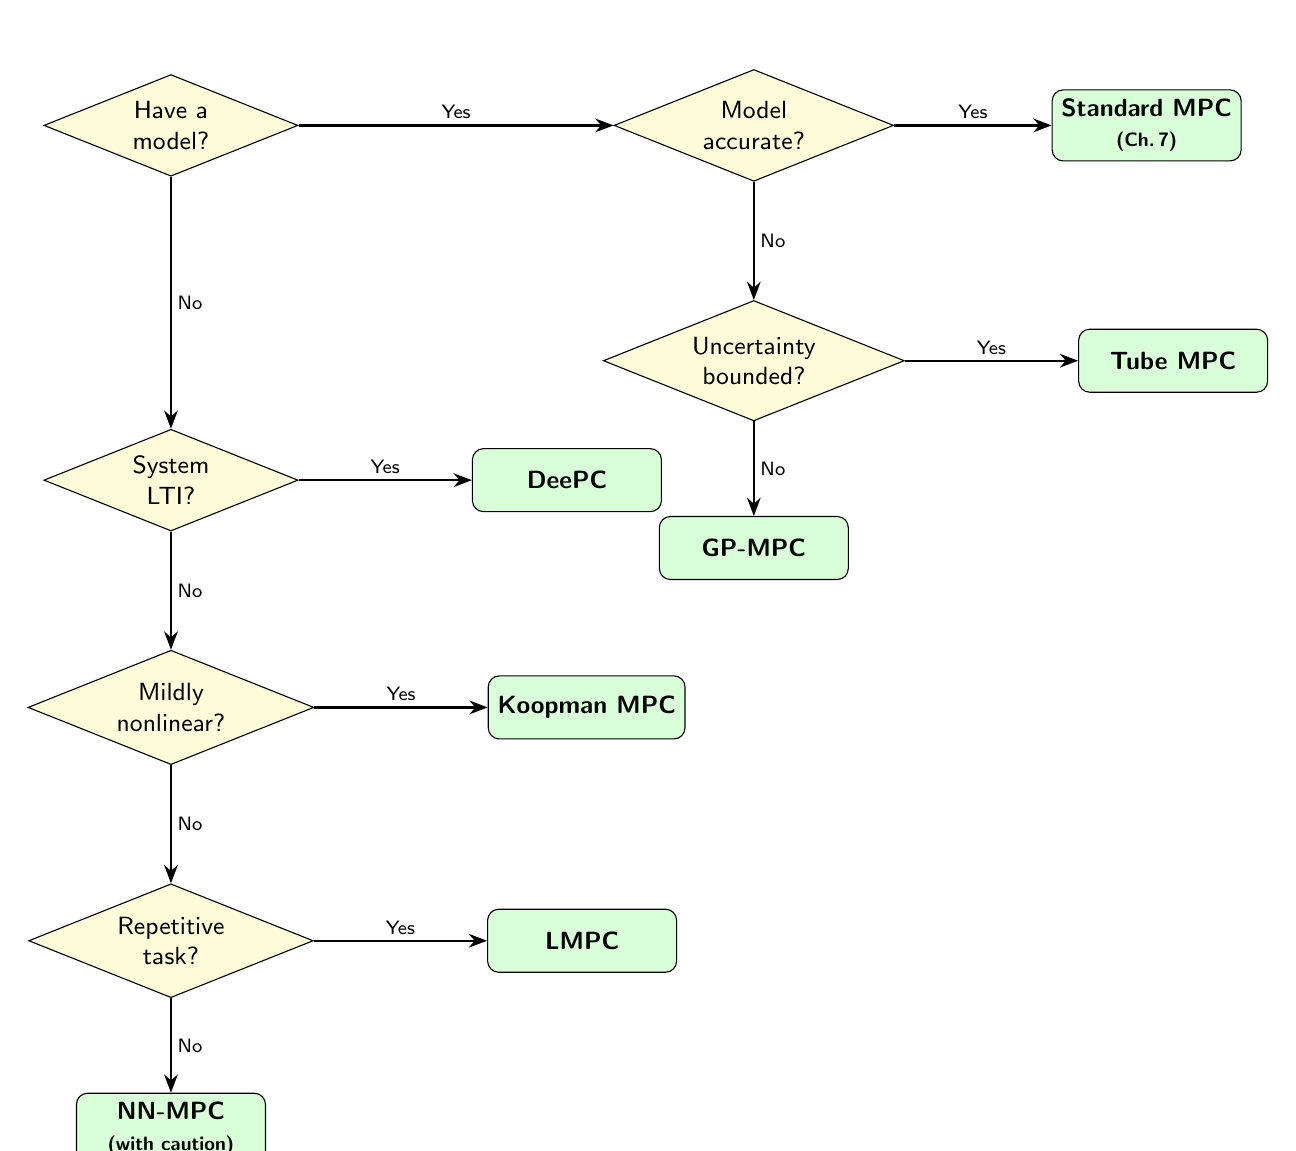
\begin{tikzpicture}[
		>=Stealth,
		node distance=0.9cm and 1.6cm,
		decision/.style={draw, diamond, aspect=2.5, fill=yellow!15,
			minimum width=2.4cm, minimum height=0.9cm, align=center,
			font=\small, inner sep=3pt},
		result/.style={draw, rounded corners=4pt, fill=green!15,
			minimum width=2.4cm, minimum height=0.8cm, align=center,
			font=\small\bfseries},
		arr/.style={->, thick},
		lbl/.style={font=\scriptsize, fill=white, inner sep=2pt},
	]
		% Decision 1: Have a model?
		\node[decision] (d1) {Have a\\model?};

		% Yes branch
		\node[decision, right=4cm of d1] (d2) {Model\\accurate?};
		\draw[arr] (d1.east) -- node[lbl, above] {Yes} (d2.west);

		\node[result, right=2.0cm of d2] (r1) {Standard MPC\\{\scriptsize (Ch.\,7)}};
		\draw[arr] (d2.east) -- node[lbl, above] {Yes} (r1.west);

		\node[decision, below=1.5cm of d2] (d2b) {Uncertainty\\bounded?};
		\draw[arr] (d2.south) -- node[lbl, right] {No} (d2b.north);

		\node[result, right=2.2cm of d2b] (r2) {Tube MPC};
		\draw[arr] (d2b.east) -- node[lbl, above] {Yes} (r2.west);

		\node[result, below=1.2cm of d2b] (r3) {GP-MPC};
		\draw[arr] (d2b.south) -- node[lbl, right] {No} (r3.north);

		% No branch
		\node[decision, below=3.2cm of d1] (d3) {System\\LTI?};
		\draw[arr] (d1.south) -- node[lbl, right] {No} (d3.north);

		\node[result, right=2.2cm of d3] (r4) {DeePC};
		\draw[arr] (d3.east) -- node[lbl, above] {Yes} (r4.west);

		\node[decision, below=1.5cm of d3] (d4) {Mildly\\nonlinear?};
		\draw[arr] (d3.south) -- node[lbl, right] {No} (d4.north);

		\node[result, right=2.2cm of d4] (r5) {Koopman MPC};
		\draw[arr] (d4.east) -- node[lbl, above] {Yes} (r5.west);

		\node[decision, below=1.5cm of d4] (d5) {Repetitive\\task?};
		\draw[arr] (d4.south) -- node[lbl, right] {No} (d5.north);

		\node[result, right=2.2cm of d5] (r6) {LMPC};
		\draw[arr] (d5.east) -- node[lbl, above] {Yes} (r6.west);

		\node[result, below=1.2cm of d5] (r7) {NN-MPC\\{\scriptsize (with caution)}};
		\draw[arr] (d5.south) -- node[lbl, right] {No} (r7.north);
	\end{tikzpicture}
	\caption{Decision flowchart for selecting an MPC method. Starting from the availability of a model, the flowchart guides the practitioner through a sequence of questions about model accuracy, uncertainty structure, system linearity, and task structure. Each terminal node (green) indicates the recommended approach.}
	\label{fig:method_flowchart}
\end{figure}


\begin{summarybox}{Comparison of Learning-Based MPC Methods}
	\begin{center}
		\resizebox{\linewidth}{!}{%
		\small
		\begin{tabular}{l c c c c c}
			\toprule
			& \emph{GP-MPC} & \emph{Koopman} & \emph{DeePC} & \emph{LMPC} & \emph{NN-MPC} \\
			\midrule
			Nominal model needed? & Yes & No & No & Yes & No \\
			System class & Nonlinear & Mildly NL & LTI & Any & Nonlinear \\
			Online computation & NLP (mild) & QP & QP & QP/NLP & NLP (severe) \\
			Uncertainty quantified? & Yes & No & Indirectly & No & No \\
			Guarantees & Chance (1-step) & Approx.\ linear & LTI equiv. & Recur.\ feas. & Weak \\
			YALMIP usable? & Yes & Yes & Yes & Yes & No \\
			\bottomrule
		\end{tabular}%
		}
	\end{center}
\end{summarybox}

\begin{alertbox}{Assumptions and Limitations}
	Every learning-based method introduces assumptions beyond those of standard MPC:
	\begin{itemize}[noitemsep]
		\item GP-MPC assumes the residual is a smooth function (kernel choice).
		\item Koopman MPC assumes the dictionary spans the relevant observables.
		\item DeePC assumes LTI dynamics (or mild nonlinearity with regularisation).
		\item LMPC assumes the task is repetitive with fixed initial and terminal conditions.
		\item NN-MPC provides no formal constraint or stability guarantees.
	\end{itemize}
	The choice of method must be guided by the problem structure, the available data, and the required guarantees.
\end{alertbox}


%% ============================================================
%%  SECTION 9: SUMMARY
%% ============================================================
\section{Summary}
\label{sec:learning_summary}

\begin{summarybox}{Chapter Summary}
	This chapter introduced five methods for combining learning with MPC:
	\begin{enumerate}
		\item \emph{GP-MPC}: learns a probabilistic residual model; provides adaptive constraint tightening via chance constraints.
		\item \emph{Koopman MPC}: lifts nonlinear dynamics to a linear space via a data-driven dictionary; reduces to a standard QP.
		\item \emph{DeePC}: uses raw input--output data in a Hankel-matrix formulation; bypasses system identification entirely.
		\item \emph{LMPC}: exploits data from repeated task executions to expand the safe set and improve performance.
		\item \emph{NN-MPC}: uses neural networks for dynamics learning; expressive but non-convex and harder to certify.
	\end{enumerate}
	The key trade-off is between expressiveness and tractability. Koopman MPC and DeePC preserve the QP structure of standard linear MPC, making them directly suitable for real-time implementation with existing solvers. GP-MPC is an NLP but admits effective convex approximations. NN-MPC is the most expressive but also the least tractable, producing non-convex NLPs with limited formal guarantees.
\end{summarybox}

\subsection*{Further Reading}

\begin{itemize}[noitemsep]
	\item Willems, Rapisarda, Markovsky \& De Moor (2005): the Fundamental Lemma~\cite{Willems2005}.
	\item Rasmussen \& Williams (2006): the standard textbook on Gaussian processes~\cite{Rasmussen2006}.
	\item Hewing, Wabersich, Menner \& Zeilinger (2020): a survey of learning-based MPC~\cite{Hewing2020}.
	\item Coulson, Lygeros \& D\"orfler (2019): the original DeePC paper~\cite{Coulson2019}.
	\item Rosolia \& Borrelli (2018): Learning MPC for iterative tasks~\cite{Rosolia2018}.
	\item Korda \& Mezi\'c (2018): Koopman-based linear predictors for nonlinear MPC~\cite{Korda2018}.
	\item D\"orfler, Coulson \& Markovsky (2023): bridging data-driven and model-based control via regularisation~\cite{Dorfler2023}.
\end{itemize}


%% ============================================================
%%  EXERCISES
%% ============================================================
\section*{Exercises}

\begin{enumerate}
	\item \emph{GP Regression (hand-worked).}
	\begin{enumerate}
		\item Given 4 training points $\{(0, 0.1),\; (1, 0.9),\; (2, 0.15),\; (3, -0.8)\}$ and the SE kernel with $\sigma_f = 1$, $\ell = 1.5$, $\sigma_n = 0.1$, compute the $4 \times 4$ Gram matrix $K$.
		\item Compute the predictive mean $\mu_*$ and variance $\sigma_*^2$ at $x_* = 1.5$.
		\item If this GP models a dynamics residual and the state constraint is $|x| \le 5$, compute the tightened constraint at $x_* = 1.5$ for $\delta = 0.025$ (i.e.\ a 97.5\% chance constraint).
		\item Discuss qualitatively: what happens to $\sigma_*^2$ as the number of training points near $x_*$ increases?
	\end{enumerate}

	\item \emph{EDMD Identification (hand-worked).}
	\begin{enumerate}
		\item For $x_{k+1} = 0.5\,x_k + 0.2\,x_k^2 + u_k$ with dictionary $\Psi(x) = [x,\; x^2]^\top$, generate 6 transitions from $x_0 = 0$ with inputs $u = [0.5,\; -0.3,\; 0.8,\; -0.5,\; 0.1,\; -0.2]$.
		\item Construct the lifted data matrices $Z$, $Z'$, $U$ and solve for $[A_K,\; B_K]$ via the pseudoinverse.
		\item Compare the one-step prediction error of the Koopman model to that of a linearisation about the origin ($x_{k+1} \approx 0.5\,x_k + u_k$) at the test point $x = 2$, $u = 0$.
	\end{enumerate}

	\item \emph{DeePC: Hankel Matrix Construction.}
	\begin{enumerate}
		\item For the first-order system $y_{k+1} = 0.9\,y_k + u_k$ with $T = 10$ data points and $L = 4$, construct the Hankel matrices $\mathcal{H}_4(u^d)$ and $\mathcal{H}_4(y^d)$.
		\item Verify the rank condition for PE of order $L + n = 5$.
		\item Write out the DeePC QP~\eqref{eq:deepc_qp} explicitly (decision variables, cost, constraints) for $T_\text{ini} = 1$, $N = 3$.
		\item Compute the minimum data length $T$ required for PE with system orders $n = 1, 2, 4$ and input dimension $m = 1$, assuming $L = 12$.
	\end{enumerate}

	\item \emph{DeePC vs Model-Based MPC (MATLAB).}
	\begin{enumerate}
		\item Implement DeePC for the double integrator (Section~\ref{sec:deepc_double_int}) using the code provided.
		\item Implement standard model-based MPC (Chapter~7 formulation) for the same system with the same cost matrices and constraints.
		\item Compare the closed-loop trajectories. Are they identical? Explain.
		\item Corrupt the data with additive noise: $u_k^d \leftarrow u_k^d + \varepsilon_k$, $y_k^d \leftarrow y_k^d + \eta_k$, with $\varepsilon_k, \eta_k \sim \mathcal{N}(0, \sigma^2)$ for $\sigma \in \{0.01,\; 0.1,\; 0.5\}$. How does DeePC performance degrade? How do the regularisation parameters $\lambda_g$ and $\lambda_\sigma$ help?
	\end{enumerate}

	\item \emph{LMPC (scalar computation).}
	\begin{enumerate}
		\item For $x_{k+1} = x_k + u_k$, $|u_k| \le 1$, $x_0 = 3$, $x_F = 0$, with stage cost $\ell = 1$: compute the trajectory for iteration~0 using $u_k = -0.5$ at every step.
		\item Construct the safe set $\mathcal{SS}^0$ and the cost-to-go $Q^0(x)$ for each state in the trajectory.
		\item With $N = 2$, show that iteration~1 can achieve $u_k = -1$ (i.e.\ saturated input) and reach the origin faster. Compute the cost $J^{(1)}$.
		\item What is the theoretical minimum cost (minimum number of steps)? How many LMPC iterations are needed to achieve it?
	\end{enumerate}

	\item \emph{Method Selection (conceptual).} For each scenario, argue which learning-based MPC approach is most appropriate and explain your reasoning:
	\begin{enumerate}
		\item A chemical reactor with well-understood reaction kinetics but unknown and time-varying heat loss to the environment.
		\item An autonomous car performing laps on a race circuit, where the track layout is fixed but tyre grip varies with temperature.
		\item A power electronics converter whose input--output behaviour has been measured extensively, and the internal dynamics are believed to be linear.
		\item A soft robotic arm with complex, highly nonlinear dynamics that are difficult to model from first principles.
	\end{enumerate}
\end{enumerate}

	\chapter{Course Conclusion and Further Topics\texorpdfstring{$^{(*)}$}{(*)}}
\label{chap:conclusion}

The course progressed from the \emph{Linear Quadratic Regulator (LQR)} through \emph{Model Predictive Control (MPC)} with explicit constraint handling, to \emph{State Estimation} and \emph{Disturbance Modelling} for offset-free tracking in the presence of noise and uncertainty.

The structure presented here---\emph{MPC + Estimator + Target Calculator}---is the standard architecture for linear MPC in process control. We omitted several advanced topics; this chapter provides pointers for further study.

\section{Rigorous Stability Analysis}
In the basic MPC formulation without a terminal set constraint, the \emph{Terminal Cost} ($x_N^\top P x_N$) encourages stability but does not mathematically \textit{guarantee} it for constrained systems. (Chapter~\ref{chap:linear_mpc}, Section~\ref{sec:mpc_stability_theory} provides the rigorous proof when the terminal set \emph{is} included.)

Rigorous MPC theory relies on Lyapunov analysis. To prove stability, one must often include a \emph{Terminal Set Constraint} ($x_N \in \mathcal{X}_f$) in the optimisation. This forces the state to land in a \emph{safe haven} (a Positive Invariant Set, meaning that once the trajectory enters the terminal set, it remains inside) at the end of the horizon, ensuring recursive feasibility.

The fundamental reference for this topic is Mayne et al.~\cite{Mayne2000}.

\section{Robust MPC}
Robust MPC, specifically the Tube MPC approach, is covered in detail in Chapter~\ref{chap:tube_mpc}. The reader is referred there for the full development including Minkowski sums, Pontryagin differences, minimal robust positively invariant sets, and constraint tightening.

\section{Nonlinear MPC (NMPC)}
Nonlinear MPC is covered in detail in Chapter~\ref{chap:nmpc}. The reader is referred there for direct transcription methods, the CasADi/IPOPT workflow, successive convexification (SCvx), GuSTO, a powered rocket landing application, and Real-Time Iteration.

\section{Real-Time Implementation and Embedded MPC}
In our examples, we used solvers such as MATLAB's \texttt{quadprog} or the open-source solver IPOPT (accessed via CasADi or other interfaces), which are sufficient for offline simulations but insufficient for millisecond-level control on microcontrollers or DSPs. Deploying MPC on embedded hardware requires specialised techniques:
\begin{itemize}
	\item \textbf{Explicit MPC (Multiparametric Programming)~\cite{Bemporad2002}:} For small systems, we can pre-calculate the solution offline. The result is a lookup table of affine gains, one per polyhedral region of the state space. On the chip, the ``optimisation'' reduces to \texttt{if-else} checks to find the correct region, requiring microseconds to execute. Section~\ref{sec:explicit_mpc} develops this approach with worked examples and MPT3 code.
	\item \textbf{Code Generation:} Tools like \href{https://acado.github.io/}{ACADO}, \href{https://cvxgen.com/}{CVXGEN}, or \href{https://osqp.org/}{OSQP} generate highly optimised, library-free C-code specifically tailored to the structure of the MPC problem, allowing convex MPC to run on standard automotive ECUs.
\end{itemize}

The fundamental reference for explicit MPC is Bemporad et al.~\cite{Bemporad2002}.

\section{Data-Driven and Learning-Based MPC}
Data-driven and learning-based MPC methods are covered in detail in Chapter~\ref{chap:learning_mpc}. The reader is referred there for GP-MPC, Koopman MPC, DeePC (including Willems' Fundamental Lemma), and Learning MPC, with full derivations, worked examples, and MATLAB/YALMIP implementations.


	\begin{appendices}
		% ============================================================
%  File: Appendix1.tex (Linear Algebra)
%  \input this file as an appendix chapter.
%  All environments reference the existing preamble.
%  British English throughout.
% ============================================================

\chapter{Linear Algebra: A Self-Study Reference}
\label{app:linalg}

This appendix provides a concise but complete review of the linear
algebra concepts used throughout these lecture notes.  Each topic is
presented with a formal definition, worked examples by hand, and the
corresponding MATLAB commands so that you can verify every result
interactively.  No prior knowledge beyond basic school-level algebra is
assumed.

All MATLAB code in this appendix can be typed directly into the MATLAB
Command Window or saved as a script.  Matrices are entered row by row,
with semicolons separating rows and commas (or spaces) separating
elements within a row.

% =============================================================
\section{Scalars, Vectors, and Matrices}
\label{sec:app_basics}
% =============================================================

\begin{defnbox}{Scalar}
	A \textbf{scalar} is a single real (or complex) number, denoted by a
	lower-case italic letter, e.g.\ $a = 3.7$.
\end{defnbox}

\begin{defnbox}{Vector}
	A \textbf{column vector} of size $n$ is an ordered list of $n$ scalars
	arranged vertically:
	\[
	{x} =
	\begin{bmatrix} x_1 \\ x_2 \\ \vdots \\ x_n \end{bmatrix}
	\in \mathbb{R}^n.
	\]
	A {row vector} is the transpose of a column vector:
	${x}^\top = [x_1,\; x_2,\; \ldots,\; x_n]$.  Unless stated
	otherwise, \emph{vector} means column vector in these notes.
\end{defnbox}

\begin{defnbox}{Matrix}
	An $m \times n$ \textbf{matrix} has $m$ rows and $n$ columns:
	\[
	A =
	\begin{bmatrix}
		a_{11} & a_{12} & \cdots & a_{1n} \\
		a_{21} & a_{22} & \cdots & a_{2n} \\
		\vdots & \vdots & \ddots & \vdots \\
		a_{m1} & a_{m2} & \cdots & a_{mn}
	\end{bmatrix}
	\in \mathbb{R}^{m \times n}.
	\]
	The element in row $i$ and column $j$ is written $a_{ij}$ or
	$[A]_{ij}$.  A \textbf{square matrix} has $m = n$.
\end{defnbox}

\begin{notebox}{MATLAB notation}
	MATLAB uses \texttt{(i,j)} indexing for elements, starting from 1:
	\texttt{A(i,j)} returns $a_{ij}$.  Size is queried with
	\texttt{size(A)}, which returns \texttt{[m n]}.
\end{notebox}

\begin{examplebox}{Entering matrices and vectors in MATLAB}
	\begin{lstlisting}[language=Matlab]
		% Column vector
		x = [2; -1; 4];       % 3x1, semicolons separate rows
		
		% Row vector
		y = [5, 0, -3];       % 1x3, commas separate elements
		
		% 3x3 matrix
		A = [1, 2, 3;
		4, 5, 6;
		7, 8, 9];
		
		% Access element in row 2, column 3
		a23 = A(2,3)          % returns 6
		
		% Query dimensions
		[m, n] = size(A)      % m=3, n=3
	\end{lstlisting}
	
	\solution
	Running the code above sets \texttt{a23 = 6} and confirms $A$ is
	$3\times 3$.  Vectors are simply matrices where one dimension equals 1.
\end{examplebox}

% =============================================================
\section{Special Matrices}
\label{sec:app_special}
% =============================================================

Several matrix types appear repeatedly in MPC formulations and are
worth knowing by name.

\begin{defnbox}{Important Special Matrices}
	\begin{itemize}[noitemsep]
		\item \textbf{Zero matrix} $0_{m\times n}$: all entries are
		zero.
		\item \textbf{Identity matrix} $I_n$: square, ones on the main
		diagonal, zeros elsewhere; $[I_n]_{ij} = 1$ if $i=j$, else $0$.
		\item \textbf{Diagonal matrix}: square, all off-diagonal entries are
		zero; written $\mathrm{diag}(d_1, d_2, \ldots, d_n)$.
		\item \textbf{Symmetric matrix}: square, $A = A^\top$, i.e.\
		$a_{ij} = a_{ji}$ for all $i,j$.
		\item \textbf{Positive definite matrix}: symmetric $A$ such that
		${x}^\top A {x} > 0$ for all
		${x} \neq 0$.  Written $A \succ 0$.
		\item \textbf{Positive semi-definite matrix}: symmetric $A$ such that
		${x}^\top A {x} \geq 0$.  Written $A \succeq 0$.
	\end{itemize}
\end{defnbox}

\begin{notebox}{Why positive definiteness matters in MPC}
	The cost matrices $Q$ and $R$ in the MPC objective must satisfy
	$Q \succeq 0$ and $R \succ 0$ for the optimisation problem to be
	well-posed (bounded below with a unique minimiser).
\end{notebox}

\begin{examplebox}{Special matrices in MATLAB}
	\begin{lstlisting}[language=Matlab]
		n = 4;
		Z  = zeros(n);          % 4x4 zero matrix
		I  = eye(n);            % 4x4 identity matrix
		D  = diag([1, 2, 3, 4]);% 4x4 diagonal matrix
		
		% Check symmetry
		A  = [4, 2; 2, 3];
		issymmetric(A)          % returns 1 (true)
		
		% Check positive definiteness via eigenvalues
		ev = eig(A)             % all positive => A is positive definite
	\end{lstlisting}
	\solution
	\texttt{eig(A)} returns \texttt{[1.4384; 5.5616]}, both positive,
	confirming $A \succ 0$.
\end{examplebox}

% =============================================================
\section{Matrix Addition and Subtraction}
\label{sec:app_addsubtract}
% =============================================================

\begin{defnbox}{Addition and Subtraction}
	Two matrices $A, B \in \mathbb{R}^{m \times n}$ of the \emph{same
		size} are added (or subtracted) element by element:
	\[
	[A \pm B]_{ij} = a_{ij} \pm b_{ij}.
	\]
	Addition with matrices of different sizes is \textbf{not defined}.
\end{defnbox}

\textbf{Properties of matrix addition:}
\begin{itemize}[noitemsep]
	\item Commutativity: $A + B = B + A$
	\item Associativity: $(A + B) + C = A + (B + C)$
	\item Identity element: $A + 0 = A$
	\item Distributivity over scalars: $\alpha(A+B) = \alpha A + \alpha B$
\end{itemize}

\begin{examplebox}{Matrix addition and subtraction by hand and in MATLAB}
	Let
	\[
	A = \begin{bmatrix} 1 & 3 \\ -2 & 4 \end{bmatrix},
	\qquad
	B = \begin{bmatrix} 5 & -1 \\ 0 & 2 \end{bmatrix}.
	\]
	Compute $A + B$, $A - B$, and $3A$.
	
	\solution
	\[
	A + B =
	\begin{bmatrix} 1+5 & 3-1 \\ -2+0 & 4+2 \end{bmatrix}
	= \begin{bmatrix} 6 & 2 \\ -2 & 6 \end{bmatrix},
	\]
	\[
	A - B =
	\begin{bmatrix} 1-5 & 3+1 \\ -2-0 & 4-2 \end{bmatrix}
	= \begin{bmatrix} -4 & 4 \\ -2 & 2 \end{bmatrix},
	\]
	\[
	3A =
	\begin{bmatrix} 3 & 9 \\ -6 & 12 \end{bmatrix}.
	\]
	
	\begin{lstlisting}[language=Matlab]
		A = [1, 3; -2, 4];
		B = [5, -1; 0, 2];
		
		ApB = A + B     % [6  2; -2  6]
		AmB = A - B     % [-4  4; -2  2]
		threeA = 3*A    % [3  9; -6  12]
	\end{lstlisting}
\end{examplebox}

% =============================================================
\section{Matrix Transpose}
\label{sec:app_transpose}
% =============================================================

\begin{defnbox}{Transpose}
	The \textbf{transpose} of $A \in \mathbb{R}^{m \times n}$ is the
	matrix $A^\top \in \mathbb{R}^{n \times m}$ obtained by swapping rows
	and columns: $[A^\top]_{ij} = a_{ji}$.
\end{defnbox}

\textbf{Useful transpose identities:}
\begin{align}
	(A^\top)^\top &= A \label{eq:t1}\\
	(A + B)^\top  &= A^\top + B^\top \label{eq:t2}\\
	(AB)^\top     &= B^\top A^\top \label{eq:t3}\\
	(\alpha A)^\top &= \alpha A^\top \label{eq:t4}
\end{align}

Identity \eqref{eq:t3} is the most frequently used and most easily
forgotten: note the \emph{reversed} order.

\begin{examplebox}{Transpose in MATLAB}
	\begin{lstlisting}[language=Matlab]
		A  = [1, 2, 3; 4, 5, 6];   % 2x3 matrix
		At = A'                      % 3x2 transpose
		
		% Verify (AB)' = B'A'
		B  = [1, 0; -1, 2; 3, 1];  % 3x2 so that AB is defined
		lhs = (A*B)'
		rhs = B' * A'
		isequal(lhs, rhs)           % returns 1 (true)
	\end{lstlisting}
	\solution
	\texttt{At} is the $3\times2$ matrix with rows \texttt{[1 4]},
	\texttt{[2 5]}, \texttt{[3 6]}.  MATLAB confirms the identity.
	
	\textbf{Warning:} in MATLAB, \texttt{A'} computes the
	\emph{conjugate} (Hermitian) transpose.  For real matrices this makes
	no difference.  For complex matrices use \texttt{A.'} (dot-transpose)
	if you want the non-conjugate transpose.
\end{examplebox}

% =============================================================
\section{Matrix--Matrix Multiplication}
\label{sec:app_matmat}
% =============================================================

\begin{defnbox}{Matrix Multiplication}
	If $A \in \mathbb{R}^{m \times p}$ and $B \in \mathbb{R}^{p \times n}$
	(the inner dimensions must match), their product
	$C = AB \in \mathbb{R}^{m \times n}$ is defined by
	\[
	c_{ij} = \sum_{k=1}^{p} a_{ik}\, b_{kj},
	\qquad i = 1,\ldots,m,\quad j = 1,\ldots,n.
	\]
	In words: the $(i,j)$ entry of $C$ is the \emph{dot product} of the
	$i$-th row of $A$ with the $j$-th column of $B$.
\end{defnbox}

\begin{alertbox}{Matrix multiplication is NOT commutative}
	In general $AB \neq BA$.  The product $BA$ may not even be defined if
	$A$ and $B$ are not square.  Always check dimension compatibility
	before multiplying: an $m\times p$ matrix times a $p \times n$ matrix
	gives an $m \times n$ result.
\end{alertbox}

\textbf{Properties:}
\begin{itemize}[noitemsep]
	\item Associativity: $(AB)C = A(BC)$
	\item Distributivity: $A(B+C) = AB + AC$
	\item Identity: $AI = IA = A$
	\item Scalar: $(\alpha A)B = A(\alpha B) = \alpha(AB)$
\end{itemize}

\begin{examplebox}{Matrix--matrix multiplication by hand and in MATLAB}
	Let
	\[
	A = \begin{bmatrix} 1 & 2 \\ 3 & 4 \end{bmatrix},
	\qquad
	B = \begin{bmatrix} 5 & 6 \\ 7 & 8 \end{bmatrix}.
	\]
	Compute $AB$ and $BA$ and confirm they differ.
	
	\solution
	\[
	AB =
	\begin{bmatrix}
		1\cdot5 + 2\cdot7 & 1\cdot6 + 2\cdot8 \\
		3\cdot5 + 4\cdot7 & 3\cdot6 + 4\cdot8
	\end{bmatrix}
	=
	\begin{bmatrix} 19 & 22 \\ 43 & 50 \end{bmatrix},
	\]
	\[
	BA =
	\begin{bmatrix}
		5\cdot1 + 6\cdot3 & 5\cdot2 + 6\cdot4 \\
		7\cdot1 + 8\cdot3 & 7\cdot2 + 8\cdot4
	\end{bmatrix}
	=
	\begin{bmatrix} 23 & 34 \\ 31 & 46 \end{bmatrix}.
	\]
	Clearly $AB \neq BA$.
	
	\begin{lstlisting}[language=Matlab]
		A  = [1, 2; 3, 4];
		B  = [5, 6; 7, 8];
		
		AB = A * B          % [19 22; 43 50]
		BA = B * A          % [23 34; 31 46]
		isequal(AB, BA)     % returns 0 (false) -- not commutative
	\end{lstlisting}
\end{examplebox}

\begin{examplebox}{Non-square matrix multiplication}
	\[
	A = \begin{bmatrix} 1 & 0 & -1 \\ 2 & 3 & 1 \end{bmatrix} \in
	\mathbb{R}^{2\times 3}, \qquad
	B = \begin{bmatrix} 2 \\ -1 \\ 4 \end{bmatrix} \in \mathbb{R}^{3\times 1}.
	\]
	Compute $AB$ (which exists) and state why $BA$ does not exist.
	
	\solution
	$A$ is $2\times 3$ and $B$ is $3\times 1$: inner dimensions both equal
	3, so $AB \in \mathbb{R}^{2\times 1}$:
	\[
	AB =
	\begin{bmatrix}
		1\cdot2 + 0\cdot(-1) + (-1)\cdot4 \\
		2\cdot2 + 3\cdot(-1) + 1\cdot4
	\end{bmatrix}
	=
	\begin{bmatrix} -2 \\ 5 \end{bmatrix}.
	\]
	$BA$ would require $B$ ($3\times1$) times $A$ ($2\times3$): inner
	dimensions are $1 \neq 2$, so $BA$ is \textbf{undefined}.
	
	\begin{lstlisting}[language=Matlab]
		A = [1, 0, -1; 2, 3, 1];
		B = [2; -1; 4];
		AB = A * B          % [-2; 5]
		BA = B * A          % Error: inner matrix dimensions must agree
	\end{lstlisting}
\end{examplebox}

% =============================================================
\section{Matrix--Vector Multiplication}
\label{sec:app_matvec}
% =============================================================

Matrix--vector multiplication is a special case of matrix--matrix
multiplication where $n=1$, but it has a particularly important
geometric interpretation: $A{x}$ transforms the vector
${x}$ into a new vector in a (possibly different) space.

\begin{defnbox}{Matrix--Vector Product}
	For $A \in \mathbb{R}^{m\times n}$ and
	${x} \in \mathbb{R}^n$:
	\[
	{y} = A{x}, \qquad
	y_i = \sum_{j=1}^{n} a_{ij}\, x_j, \quad i = 1,\ldots,m.
	\]
	Equivalently, $A{x}$ is a {linear combination} of the
	columns of $A$ with coefficients given by the entries of ${x}$:
	\[
	A{x} = x_1 {a}_1 + x_2 {a}_2 + \cdots
	+ x_n {a}_n,
	\]
	where ${a}_j$ denotes the $j$-th column of $A$.
\end{defnbox}

In state-space control the plant update $x_{k+1} = Ax_k + Bu_k$ is
nothing more than two matrix--vector products added together.

\begin{examplebox}{Matrix--vector multiplication by hand and in MATLAB}
	Given the state-space matrices
	\[
	A = \begin{bmatrix} 0.9 & 0.1 \\ 0 & 0.8 \end{bmatrix},
	\quad
	B = \begin{bmatrix} 0.1 \\ 0.5 \end{bmatrix},
	\quad
	x_k = \begin{bmatrix} 2 \\ -1 \end{bmatrix},
	\quad
	u_k = 3,
	\]
	compute the next state $x_{k+1} = Ax_k + Bu_k$.
	
	\solution
	\[
	Ax_k =
	\begin{bmatrix} 0.9\cdot2 + 0.1\cdot(-1) \\ 0\cdot2 + 0.8\cdot(-1)
	\end{bmatrix}
	= \begin{bmatrix} 1.7 \\ -0.8 \end{bmatrix},
	\qquad
	Bu_k =
	\begin{bmatrix} 0.3 \\ 1.5 \end{bmatrix},
	\]
	\[
	x_{k+1} = \begin{bmatrix} 1.7 \\ -0.8 \end{bmatrix}
	+ \begin{bmatrix} 0.3 \\ 1.5 \end{bmatrix}
	= \begin{bmatrix} 2.0 \\ 0.7 \end{bmatrix}.
	\]
	
	\begin{lstlisting}[language=Matlab]
		A  = [0.9, 0.1; 0, 0.8];
		B  = [0.1; 0.5];
		xk = [2; -1];
		uk = 3;
		
		xk1 = A*xk + B*uk    % [2.0; 0.7]
	\end{lstlisting}
\end{examplebox}

% =============================================================
\section{The Inverse of a Matrix}
\label{sec:app_inverse}
% =============================================================

\begin{defnbox}{Matrix Inverse}
	A square matrix $A \in \mathbb{R}^{n\times n}$ is \textbf{invertible}
	(or \textbf{non-singular}) if there exists a matrix
	$A^{-1} \in \mathbb{R}^{n\times n}$ such that
	\[
	A A^{-1} = A^{-1} A = I_n.
	\]
	If no such matrix exists, $A$ is called \textbf{singular}.
\end{defnbox}

\begin{defnbox}{Conditions for Invertibility}
	A square matrix $A$ is invertible if and only if any one of the
	following equivalent conditions holds:
	\begin{itemize}[noitemsep]
		\item $\det(A) \neq 0$ (see Section~\ref{sec:app_det});
		\item all eigenvalues of $A$ are non-zero
		(see Section~\ref{sec:app_eig});
		\item the columns (or rows) of $A$ are linearly independent;
		\item the equation $A{x} = 0$ has only the trivial
		solution ${x} = 0$.
	\end{itemize}
\end{defnbox}

\textbf{Useful inverse identities:}
\begin{align}
	(A^{-1})^{-1} &= A \\
	(AB)^{-1}     &= B^{-1} A^{-1} \quad \text{(reversed order)} \\
	(A^\top)^{-1} &= (A^{-1})^\top \\
	(\alpha A)^{-1} &= \tfrac{1}{\alpha} A^{-1}
\end{align}

\textbf{Inverse of a $2\times2$ matrix} by hand:
\[
A = \begin{bmatrix} a & b \\ c & d \end{bmatrix}
\implies
A^{-1} = \frac{1}{ad - bc}
\begin{bmatrix} d & -b \\ -c & a \end{bmatrix}.
\]

\begin{examplebox}{Computing the inverse by hand and in MATLAB}
	Let
	\[
	A = \begin{bmatrix} 3 & 1 \\ 5 & 2 \end{bmatrix}.
	\]
	Find $A^{-1}$ and verify $AA^{-1} = I$.
	
	\solution
	$\det(A) = 3\cdot2 - 1\cdot5 = 1$, so
	\[
	A^{-1} = \frac{1}{1}
	\begin{bmatrix} 2 & -1 \\ -5 & 3 \end{bmatrix}
	= \begin{bmatrix} 2 & -1 \\ -5 & 3 \end{bmatrix}.
	\]
	Verification:
	\[
	AA^{-1} =
	\begin{bmatrix} 3 & 1 \\ 5 & 2 \end{bmatrix}
	\begin{bmatrix} 2 & -1 \\ -5 & 3 \end{bmatrix}
	=
	\begin{bmatrix} 6-5 & -3+3 \\ 10-10 & -5+6 \end{bmatrix}
	= \begin{bmatrix} 1 & 0 \\ 0 & 1 \end{bmatrix} = I. \checkmark
	\]
	
	\begin{lstlisting}[language=Matlab]
		A    = [3, 1; 5, 2];
		Ainv = inv(A)           % [2 -1; -5 3]
		
		% Verify
		A * Ainv                % should give eye(2)
		norm(A*Ainv - eye(2))   % numerical error, should be ~1e-15
	\end{lstlisting}
\end{examplebox}

\begin{alertbox}{Avoid \texttt{inv(A)} in numerical computations}
	Although \texttt{inv(A)} is convenient for checking results,
	numerically it is almost always better to use the backslash operator
	\texttt{A\textbackslash b} to solve $Ax = b$
	directly, without forming $A^{-1}$ explicitly.  The backslash
	operator uses LU factorisation, which is faster and more numerically
	stable than computing the full inverse.
	
	\begin{lstlisting}[language=Matlab]
		% Solve Ax = b
		b = [1; 2];
		x_inv = inv(A) * b    % slow and less accurate
		x_bs  = A \ b         % fast, numerically recommended
	\end{lstlisting}
\end{alertbox}

\begin{examplebox}{Detecting a singular matrix}
	\begin{lstlisting}[language=Matlab]
		A_sing = [1, 2; 2, 4];     % row 2 = 2 * row 1
		
		det(A_sing)                 % returns 0 => singular
		rank(A_sing)                % returns 1 (not full rank)
		cond(A_sing)                % returns Inf
		
		inv(A_sing)                 % MATLAB warns: matrix is singular
	\end{lstlisting}
	\solution
	The determinant is zero and the rank is 1 (not 2), confirming
	singularity.  MATLAB returns a matrix of \texttt{Inf} values from
	\texttt{inv} and issues a warning.  The condition number
	\texttt{cond(A)} measures how close a matrix is to being singular;
	values much larger than $10^6$ indicate near-singularity.
\end{examplebox}

% =============================================================
\section{The Determinant}
\label{sec:app_det}
% =============================================================

\begin{defnbox}{Determinant}
	The \textbf{determinant} $\det(A)$ (also written $|A|$) is a scalar
	function of a square matrix that encodes fundamental properties such as
	invertibility, volume scaling, and orientation.
	
	For a $2\times2$ matrix:
	\[
	\det\!\begin{bmatrix} a & b \\ c & d \end{bmatrix} = ad - bc.
	\]
	For a $3\times3$ matrix (cofactor expansion along the first row):
	\[
	\det\!\begin{bmatrix} a_{11} & a_{12} & a_{13} \\
		a_{21} & a_{22} & a_{23} \\
		a_{31} & a_{32} & a_{33} \end{bmatrix}
	= a_{11}(a_{22}a_{33} - a_{23}a_{32})
	- a_{12}(a_{21}a_{33} - a_{23}a_{31})
	+ a_{13}(a_{21}a_{32} - a_{22}a_{31}).
	\]
\end{defnbox}

\textbf{Key properties:}
\begin{itemize}[noitemsep]
	\item $\det(I) = 1$
	\item $\det(AB) = \det(A)\det(B)$
	\item $\det(A^\top) = \det(A)$
	\item $\det(A^{-1}) = 1/\det(A)$
	\item $\det(\alpha A) = \alpha^n \det(A)$ for $A \in \mathbb{R}^{n\times n}$
	\item $\det(A) = 0$ if and only if $A$ is singular
\end{itemize}

\begin{examplebox}{Determinant by hand and in MATLAB}
	Compute $\det(A)$ for
	\[
	A = \begin{bmatrix} 2 & -1 & 0 \\ 1 & 3 & -2 \\ 0 & 1 & 4 \end{bmatrix}.
	\]
	
	\solution
	Expanding along the first row:
	\[
	\det(A) = 2\bigl(3\cdot4 - (-2)\cdot1\bigr)
	- (-1)\bigl(1\cdot4 - (-2)\cdot0\bigr)
	+ 0\bigl(\cdots\bigr)
	= 2(14) + 1(4) = 32.
	\]
	
	\begin{lstlisting}[language=Matlab]
		A    = [2, -1, 0; 1, 3, -2; 0, 1, 4];
		d    = det(A)           % returns 32
	\end{lstlisting}
\end{examplebox}

% =============================================================
\section{The Trace}
\label{sec:app_trace}
% =============================================================

\begin{defnbox}{Trace}
	The \textbf{trace} of a square matrix $A \in \mathbb{R}^{n\times n}$
	is the sum of its diagonal elements:
	\[
	\mathrm{tr}(A) = \sum_{i=1}^{n} a_{ii} = a_{11} + a_{22} + \cdots + a_{nn}.
	\]
\end{defnbox}

\textbf{Key properties:}
\begin{itemize}[noitemsep]
	\item Linearity: $\mathrm{tr}(\alpha A + \beta B) = \alpha\,\mathrm{tr}(A) + \beta\,\mathrm{tr}(B)$
	\item Cyclic permutation: $\mathrm{tr}(ABC) = \mathrm{tr}(CAB) = \mathrm{tr}(BCA)$
	\item Transpose invariance: $\mathrm{tr}(A) = \mathrm{tr}(A^\top)$
	\item Equal to sum of eigenvalues: $\mathrm{tr}(A) = \sum_{i=1}^n \lambda_i$
\end{itemize}

The trace appears in control theory when expressing quadratic cost
functions compactly.  The MPC stage cost
${x}^\top Q {x}$ can be written as
$\mathrm{tr}(Q{x}{x}^\top)$, which is useful in
stochastic and robust formulations.

\begin{examplebox}{Trace in MATLAB}
	\begin{lstlisting}[language=Matlab]
		A = [1, 2, 3;
		4, 5, 6;
		7, 8, 9];
		
		tr = trace(A)           % 1 + 5 + 9 = 15
		
		% Verify trace equals sum of eigenvalues
		lambda = eig(A);
		sum(lambda)             % also 15 (up to numerical precision)
		
		% Cyclic property: tr(ABC) = tr(CAB)
		B = rand(3);  C = rand(3);
		abs(trace(A*B*C) - trace(C*A*B))   % ~1e-14, effectively zero
	\end{lstlisting}
	\solution
	\texttt{trace(A) = 15 = 1+5+9}.  The sum of eigenvalues agrees
	(numerically), confirming the identity.
\end{examplebox}

% =============================================================
\section{Eigenvalues and Eigenvectors}
\label{sec:app_eig}
% =============================================================

Eigenvalues and eigenvectors are central to understanding the dynamic
behaviour of linear systems.  In discrete-time state-space control,
the eigenvalues of the system matrix $A$ determine stability: the
closed-loop system $x_{k+1} = A_\mathrm{cl} x_k$ is stable if and
only if all eigenvalues of $A_\mathrm{cl}$ lie strictly inside the
unit circle.

\begin{defnbox}{Eigenvalue and Eigenvector}
	Let $A \in \mathbb{R}^{n\times n}$.  A scalar $\lambda \in \mathbb{C}$
	is an \textbf{eigenvalue} of $A$ if there exists a non-zero vector
	${v} \in \mathbb{C}^n$ such that
	\[
	A{v} = \lambda {v}.
	\]
	The vector $v$ is the corresponding \textbf{eigenvector}.
	Geometrically, $A$ does not rotate ${v}$; it only scales it by
	$\lambda$.
\end{defnbox}

\textbf{Finding eigenvalues — the characteristic equation:}

Rearranging $A{v} = \lambda{v}$ gives
$(A - \lambda I){v} = {0}$.  For a non-trivial solution
${v} \neq {0}$, the matrix $(A-\lambda I)$ must be
singular:
\[
\det(A - \lambda I) = 0.
\]
This is the \textbf{characteristic equation}, a degree-$n$ polynomial
in $\lambda$ whose $n$ roots (counting multiplicity, possibly complex)
are the eigenvalues.

\begin{examplebox}{Eigenvalues by hand for a $2\times2$ matrix}
	Find the eigenvalues of
	\[
	A = \begin{bmatrix} 3 & 1 \\ 1 & 3 \end{bmatrix}.
	\]
	
	\solution
	\[
	\det(A - \lambda I)
	= \det\begin{bmatrix} 3-\lambda & 1 \\ 1 & 3-\lambda \end{bmatrix}
	= (3-\lambda)^2 - 1 = 0.
	\]
	\[
	(3-\lambda)^2 = 1
	\implies 3 - \lambda = \pm 1
	\implies \lambda_1 = 4, \quad \lambda_2 = 2.
	\]
	Both eigenvalues are real and positive.  For a discrete-time system
	matrix, we would check $|\lambda_i| < 1$; here both are $> 1$, so this
	$A$ would represent an unstable open-loop plant.
	
	\begin{lstlisting}[language=Matlab]
		A      = [3, 1; 1, 3];
		lambda = eig(A)         % [2; 4]
	\end{lstlisting}
\end{examplebox}

\begin{examplebox}{Eigenvectors and the full eigendecomposition}
	Using the same matrix $A = \begin{bmatrix} 3 & 1 \\ 1 & 3 \end{bmatrix}$,
	find the eigenvectors corresponding to $\lambda_1 = 4$ and
	$\lambda_2 = 2$.
	
	\solution
	\textbf{For $\lambda_1 = 4$:}
	\[
	(A - 4I)v = \begin{bmatrix} -1 & 1 \\ 1 & -1 \end{bmatrix}
	\begin{bmatrix} v_1 \\ v_2 \end{bmatrix} = 0
	\implies -v_1 + v_2 = 0 \implies v_1 = v_2.
	\]
	Choosing $v_1 = 1$: $v_1 = \tfrac{1}{\sqrt{2}}[1,\;1]^\top$
	(normalised).
	
	\textbf{For $\lambda_2 = 2$:}
	\[
	(A - 2I)v = \begin{bmatrix} 1 & 1 \\ 1 & 1 \end{bmatrix}
	v = 0
	\implies v_1 + v_2 = 0 \implies v_2 = -v_1.
	\]
	Choosing $v_1 = 1$: $v_2 = \tfrac{1}{\sqrt{2}}[1,\;-1]^\top$.
	
	\begin{lstlisting}[language=Matlab]
		A = [3, 1; 1, 3];
		
		% eig returns V (eigenvector matrix) and D (diagonal eigenvalue matrix)
		[V, D] = eig(A)
		% V: columns are eigenvectors
		% D: diagonal entries are eigenvalues
		
		% Verify A*v = lambda*v for first eigenvector
		v1     = V(:,1);
		lam1   = D(1,1);
		norm(A*v1 - lam1*v1)    % ~1e-15, effectively zero
		
		% The eigendecomposition: A = V * D * inv(V)
		norm(A - V*D*inv(V))    % ~1e-15, effectively zero
	\end{lstlisting}
\end{examplebox}

\begin{defnbox}{Eigenvalue Properties for Stability Analysis}
	For a discrete-time system $x_{k+1} = A x_k$:
	\begin{itemize}[noitemsep]
		\item \textbf{Asymptotically stable:} all eigenvalues satisfy
		$|\lambda_i| < 1$ (strictly inside the unit circle).
		\item \textbf{Marginally stable:} all $|\lambda_i| \leq 1$ and
		those on the unit circle have distinct eigenvectors.
		\item \textbf{Unstable:} at least one eigenvalue satisfies
		$|\lambda_i| > 1$.
	\end{itemize}
	For a continuous-time system $\dot{x} = Ax$, replace the unit circle
	with the left half-plane: stable iff $\mathrm{Re}(\lambda_i) < 0$.
\end{defnbox}

\begin{examplebox}{Stability check via eigenvalues in MATLAB}
	Check whether the following discrete-time system matrix is stable:
	\[
	A = \begin{bmatrix} 0.98 & 0.01 \\ 0.02 & 0.97 \end{bmatrix}.
	\]
	
	\solution
	\begin{lstlisting}[language=Matlab]
		A      = [0.98, 0.01; 0.02, 0.97];
		lambda = eig(A)             % [0.96; 0.99]
		abs_lambda = abs(lambda)    % [0.96; 0.99]
		all(abs_lambda < 1)         % returns 1 (true) => stable
		
		% Visualise on the unit circle
		theta = linspace(0, 2*pi, 200);
		figure; hold on;
		plot(cos(theta), sin(theta), 'k--');    % unit circle
		plot(real(lambda), imag(lambda), 'rx', 'MarkerSize', 10);
		axis equal; grid on;
		xlabel('Real'); ylabel('Imaginary');
		title('Eigenvalues of A');
	\end{lstlisting}
	Both eigenvalues have magnitude less than 1, so the system is
	asymptotically stable.  The plot shows both poles inside the unit
	circle.
\end{examplebox}

% =============================================================
\section{Putting It All Together: A State-Space Example}
\label{sec:app_together}
% =============================================================

This section demonstrates how all the operations above arise together
in a single state-space simulation, mirroring the structure of the MPC
plant model used throughout these notes.

\begin{examplebox}{Two-state discrete system: simulation and analysis}
	Consider the discrete-time system
	\[
	x_{k+1} = A x_k + B u_k, \qquad y_k = C x_k,
	\]
	with
	\[
	A = \begin{bmatrix} 0.9 & 0.1 \\ 0.0 & 0.8 \end{bmatrix},
	\quad
	B = \begin{bmatrix} 0.1 \\ 0.3 \end{bmatrix},
	\quad
	C = \begin{bmatrix} 1 & 0 \end{bmatrix},
	\quad
	x_0 = \begin{bmatrix} 5 \\ 2 \end{bmatrix},
	\quad u_k = 0\;\forall k.
	\]
	
	Carry out the following tasks in MATLAB:
	\begin{enumerate}[noitemsep]
		\item Confirm the system is stable.
		\item Compute $\mathrm{tr}(A)$ and $\det(A)$ and relate them to the
		eigenvalues.
		\item Simulate 20 steps and plot the output $y_k$.
	\end{enumerate}
	
	\solution
	\begin{lstlisting}[language=Matlab]
		A  = [0.9, 0.1; 0.0, 0.8];
		B  = [0.1; 0.3];
		C  = [1, 0];
		x  = [5; 2];
		N  = 20;
		
		%% 1. Stability
		lambda = eig(A);
		disp('Eigenvalues:'); disp(lambda)
		disp('Magnitudes:');  disp(abs(lambda))
		% Both < 1 => stable
		
		%% 2. Trace and determinant
		tr_A  = trace(A)          % 0.9 + 0.8 = 1.7
		det_A = det(A)            % 0.9*0.8 - 0.1*0 = 0.72
		sum_lam  = sum(lambda)    % also 1.7 = trace
		prod_lam = prod(lambda)   % also 0.72 = det
		
		%% 3. Simulation
		y = zeros(1, N);
		for k = 1:N
		y(k) = C * x;
		x    = A * x + B * 0;   % u=0
		end
		
		figure;
		stem(1:N, y, 'filled');
		xlabel('Time step k'); ylabel('y_k');
		title('Output y_k (free response, u=0)');
		grid on;
	\end{lstlisting}
	
	The output decays to zero, consistent with the stable eigenvalues
	$\lambda_1 \approx 0.9$ and $\lambda_2 = 0.8$.  Notice that
	$\mathrm{tr}(A) = \sum \lambda_i = 1.7$ and
	$\det(A) = \prod \lambda_i = 0.72$, confirming the identities from
	Sections~\ref{sec:app_trace} and \ref{sec:app_det}.
\end{examplebox}

% =============================================================
\section{Quick Reference: MATLAB Commands}
\label{sec:app_matlab_ref}
% =============================================================

\begin{center}
	\renewcommand{\arraystretch}{1.35}
	\begin{tabular}{>{\ttfamily\small}l >{\small}l >{\small}l}
		\toprule
		\normalfont\textbf{MATLAB command} & \textbf{Operation} &
		\textbf{Example} \\
		\midrule
		A + B               & Addition              & Element-wise, same size \\
		A - B               & Subtraction           & Element-wise, same size \\
		alpha * A           & Scalar multiplication & Multiplies every entry \\
		A * B               & Matrix multiplication & Inner dims must match \\
		A'                  & Transpose (conjugate) & Use \texttt{A.'} for real transpose \\
		A \textasciicircum{} n & Matrix power       & $A^n$, square $A$ only \\
		inv(A)              & Matrix inverse        & Avoid for solving $Ax=b$ \\
		A \textbackslash{} b & Solve $Ax = b$       & Preferred over \texttt{inv(A)*b} \\
		det(A)              & Determinant           & Scalar result \\
		trace(A)            & Trace                 & Sum of diagonal \\
		eig(A)              & Eigenvalues           & Column vector $\lambda$ \\
		{[}V,D{]} = eig(A)  & Eigenvectors + values & Columns of \texttt{V}, diag of \texttt{D} \\
		rank(A)             & Rank                  & Number of independent columns \\
		cond(A)             & Condition number      & Large value $\Rightarrow$ near-singular \\
		norm(A)             & 2-norm (default)      & \texttt{norm(A,1)}, \texttt{norm(A,'fro')} also available \\
		size(A)             & Dimensions            & Returns \texttt{[m n]} \\
		zeros(m,n)          & Zero matrix           & All entries 0 \\
		ones(m,n)           & Ones matrix           & All entries 1 \\
		eye(n)              & Identity matrix       & $I_n$ \\
		diag(v)             & Diagonal matrix       & \texttt{diag(A)} extracts diagonal of $A$ \\
		linspace(a,b,n)     & Equally spaced vector & $n$ points from $a$ to $b$ \\
		\bottomrule
	\end{tabular}
\end{center}

\begin{summarybox}{Linear Algebra Summary for MPC}
	\begin{enumerate}[noitemsep]
		\item \textbf{Dimensions matter:} always check that inner dimensions
		are compatible before multiplying; $A_{m\times p} \cdot
		B_{p\times n}$ gives $C_{m\times n}$.
		\item \textbf{Multiplication is not commutative:} $AB \neq BA$ in
		general; the reversed-order rule $(AB)^\top = B^\top A^\top$
		and $(AB)^{-1} = B^{-1}A^{-1}$ are essential.
		\item \textbf{Invertibility:} $A^{-1}$ exists iff $\det(A)\neq 0$
		iff all eigenvalues are non-zero.  Use \texttt{A\textbackslash
			b} rather than \texttt{inv(A)*b}.
		\item \textbf{Stability:} for discrete-time systems, check
		$|\lambda_i| < 1$ for all eigenvalues of the closed-loop
		matrix.
		\item \textbf{Trace and determinant} equal the sum and product of
		eigenvalues respectively, providing a fast sanity check.
		\item \textbf{Positive definiteness} of cost matrices $Q \succeq 0$,
		$R \succ 0$ is required for the MPC QP to be convex and
		bounded below; verify with \texttt{eig(Q)} and
		\texttt{eig(R)}.
	\end{enumerate}
\end{summarybox}
		% ============================================================
%  File: AppendixProbability.tex
%  \input this file as a second appendix chapter.
%  All environments reference the existing preamble.
%  British English throughout.
% ============================================================

\chapter{Probability and Statistics: A Self-Study Reference}
\label{app:prob}

Modern control systems — from Kalman filters and Linear Quadratic
Gaussian (LQG) regulators to stochastic MPC and Reinforcement Learning
(RL) — are built on probability theory.  This appendix introduces the
core ideas from scratch, assuming only basic school-level mathematics.
Every concept is illustrated with worked examples and
MATLAB code so that you can develop intuition interactively before
encountering these tools in the main text.

By the end of this appendix you should be comfortable with random
variables, Gaussian distributions, expectations, covariance matrices,
Bayes' theorem, and stochastic processes — the exact toolkit needed for
Chapters on Kalman filtering, LQG, stochastic MPC, and RL.

% =============================================================
\section{Why Probability in Control?}
\label{sec:app_prob_why}
% =============================================================

Every real control system operates in an uncertain environment.
Sensors do not report exact values — they add noise.  Actuators do not
deliver exactly the commanded force or voltage.  The plant model is
always an approximation of reality.  Disturbances (wind, load changes,
temperature) are not known in advance.

Deterministic control (classical PID, standard MPC) ignores this
uncertainty or handles it implicitly through robustness margins.
Probabilistic control treats uncertainty explicitly by modelling
unknown quantities as \emph{random variables} and designing controllers
that perform well \emph{on average} or with \emph{guaranteed
probability}.  The four main applications you will encounter in these
notes are:

\begin{itemize}[noitemsep]
  \item \textbf{Kalman filter}: optimal state estimator when process
        and measurement noise are Gaussian.
  \item \textbf{LQG control}: combines a Kalman filter with an LQR
        controller to minimise expected quadratic cost under Gaussian
        noise.
  \item \textbf{Stochastic MPC}: replaces hard constraints with
        chance constraints (e.g.\ satisfy a comfort bound with
        probability 0.95).
  \item \textbf{Reinforcement Learning}: the agent observes noisy
        states and learns an optimal policy by maximising expected
        cumulative reward.
\end{itemize}

% =============================================================
\section{Sample Spaces, Outcomes, and Events}
\label{sec:app_sample_space}
% =============================================================

\begin{defnbox}{Sample Space and Event}
The \textbf{sample space} $\Omega$ is the set of all possible outcomes
of a random experiment.  An \textbf{event} $A$ is any subset
$A \subseteq \Omega$.  The \textbf{probability} of event $A$, written
$P(A)$, is a number in $[0,1]$ that quantifies how likely $A$ is to
occur.
\end{defnbox}

\textbf{The three axioms of probability} (Kolmogorov, 1933):
\begin{enumerate}[noitemsep]
  \item $P(A) \geq 0$ for every event $A$.
  \item $P(\Omega) = 1$ (something always happens).
  \item If $A$ and $B$ are \emph{mutually exclusive} ($A \cap B = \emptyset$),
        then $P(A \cup B) = P(A) + P(B)$.
\end{enumerate}

From these three axioms every other rule of probability can be derived.
Key consequences:
\begin{itemize}[noitemsep]
  \item $P(\emptyset) = 0$
  \item $P(A^c) = 1 - P(A)$, where $A^c$ is the complement of $A$
  \item $P(A \cup B) = P(A) + P(B) - P(A \cap B)$ (inclusion--exclusion)
  \item $0 \leq P(A) \leq 1$
\end{itemize}

\begin{examplebox}{Sensor failure probability}
A temperature sensor fails independently on any given day with
probability $p = 0.02$.  Over a 5-day week, what is the probability
that it fails at least once?

\solution
Let $A_i$ be the event ``fails on day $i$''.  The complement is ``never
fails in 5 days'':
\[
  P(\text{never fails}) = (1-0.02)^5 = 0.98^5 \approx 0.904.
\]
Therefore:
\[
  P(\text{at least one failure}) = 1 - 0.904 = 0.096.
\]
There is roughly a 9.6\% chance of at least one failure per week.

\begin{lstlisting}[language=Matlab]
p_fail   = 0.02;
n_days   = 5;
p_none   = (1 - p_fail)^n_days    % 0.9039
p_atleast1 = 1 - p_none           % 0.0961
\end{lstlisting}
\end{examplebox}

% =============================================================
\section{Conditional Probability and Independence}
\label{sec:app_conditional}
% =============================================================

\begin{defnbox}{Conditional Probability}
The \textbf{conditional probability} of event $A$ given that event $B$
has occurred (with $P(B) > 0$) is:
\[
  P(A \mid B) = \frac{P(A \cap B)}{P(B)}.
\]
Intuitively, conditioning on $B$ restricts the sample space to $B$ and
rescales probabilities accordingly.
\end{defnbox}

\begin{defnbox}{Statistical Independence}
Events $A$ and $B$ are \textbf{independent} if knowing $B$ occurred
gives no information about $A$:
\[
  P(A \mid B) = P(A) \quad \Longleftrightarrow \quad
  P(A \cap B) = P(A)\,P(B).
\]
In Kalman filtering, process noise and measurement noise are assumed
to be mutually independent, which greatly simplifies the filter
equations.
\end{defnbox}

\begin{examplebox}{Conditional probability with a noisy sensor}
A room is occupied 70\% of the time.  When occupied, a motion sensor
triggers with probability 0.9.  When empty, it still triggers
(false alarm) with probability 0.05.  Given that the sensor triggered,
what is the probability the room is actually occupied?

\solution
Let $O$ = ``room occupied'', $T$ = ``sensor triggered''.
\[
  P(O) = 0.7,\quad P(T \mid O) = 0.9,\quad P(T \mid O^c) = 0.05.
\]
By the \textbf{law of total probability}:
\[
  P(T) = P(T\mid O)P(O) + P(T\mid O^c)P(O^c)
       = 0.9\times0.7 + 0.05\times0.3 = 0.645.
\]
By conditional probability:
\[
  P(O\mid T) = \frac{P(T\mid O)\,P(O)}{P(T)}
             = \frac{0.63}{0.645} \approx 0.977.
\]
If the sensor triggers, the room is occupied with about 97.7\%
confidence.

\begin{lstlisting}[language=Matlab]
P_O   = 0.7;
P_T_O = 0.9;    % true positive rate
P_T_Oc= 0.05;   % false alarm rate
P_Oc  = 1 - P_O;

P_T   = P_T_O*P_O + P_T_Oc*P_Oc;     % 0.6450
P_O_T = P_T_O * P_O / P_T             % 0.9767
\end{lstlisting}
\end{examplebox}

% =============================================================
\section{Bayes' Theorem}
\label{sec:app_bayes}
% =============================================================

\begin{defnbox}{Bayes' Theorem}
For events $A$ and $B$ with $P(B) > 0$:
\[
  {P(A \mid B) = \frac{P(B \mid A)\,P(A)}{P(B)}}.
\]
In words: the \textbf{posterior} probability of $A$ given evidence $B$
equals the \textbf{likelihood} $P(B\mid A)$ times the \textbf{prior}
$P(A)$, divided by the \textbf{marginal likelihood} (evidence) $P(B)$.
\end{defnbox}

Bayes' theorem is the mathematical foundation of the Kalman filter.
At every time step the filter:
\begin{enumerate}[noitemsep]
  \item Uses the prior state estimate (before the measurement).
  \item Updates it with the likelihood of the new measurement.
  \item Produces a posterior estimate that combines both sources of
        information optimally.
\end{enumerate}

This three-step pattern — prior $\to$ likelihood $\to$ posterior —
repeats at every time step and is precisely the \emph{predict--correct}
structure of the Kalman filter described in the main text.

\begin{notebox}{Bayes' theorem and the Kalman filter}
  The Kalman filter is the exact, closed-form solution to Bayes'
  theorem when all distributions are Gaussian and the system is
  linear.  For non-linear or non-Gaussian systems, approximate methods
  (Extended Kalman Filter, Unscented Kalman Filter, Particle Filter)
  are needed — all of which still implement the same Bayesian
  predict--correct cycle.
\end{notebox}

% =============================================================
\section{Random Variables}
\label{sec:app_rv}
% =============================================================

\begin{defnbox}{Random Variable}
A \textbf{random variable} (RV) $X$ is a function that assigns a
numerical value to every outcome in the sample space $\Omega$.  It
is \textbf{discrete} if it takes countably many values and
\textbf{continuous} if it takes values in a continuous range.
\end{defnbox}

\subsection{Discrete Random Variables}
\label{subsec:app_discrete}

A discrete RV is characterised by its
\textbf{probability mass function} (PMF):
\[
  p_X(x) = P(X = x), \qquad \sum_{\text{all }x} p_X(x) = 1.
\]

\begin{examplebox}{PMF of a discrete sensor reading}
A quantised position sensor reports integer values in
$\{-2,-1,0,1,2\}$ with equal probability.  Plot the PMF.

\solution
$p_X(x) = 1/5$ for each $x \in \{-2,-1,0,1,2\}$, zero elsewhere
(a uniform discrete distribution).

\begin{lstlisting}[language=Matlab]
x   = -2:2;
pmf = ones(1,5) / 5;

figure;
stem(x, pmf, 'filled', 'LineWidth', 1.5);
xlabel('Sensor reading x');
ylabel('P(X = x)');
title('PMF of quantised sensor');
ylim([0, 0.4]); grid on;
\end{lstlisting}

\end{examplebox}

\begin{figure}[htbp]
\centering
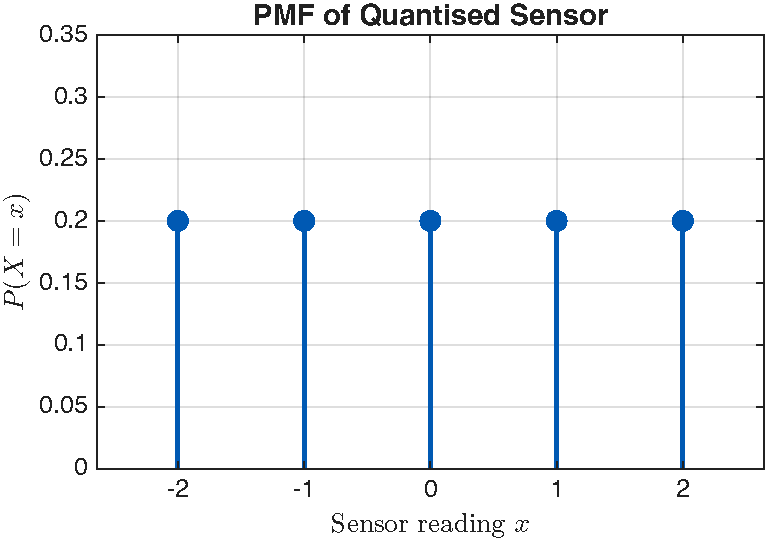
\includegraphics[width=0.65\textwidth]{Figures/fig_app_pmf_discrete.pdf}
\caption{PMF of the quantised sensor.  Each of the five possible readings has equal probability $1/5$.}
\label{fig:app_pmf_discrete}
\end{figure}

\subsection{Continuous Random Variables}
\label{subsec:app_continuous}

A continuous RV is characterised by its
\textbf{probability density function} (PDF) $f_X(x)$, defined so that:
\[
  P(a \leq X \leq b) = \int_a^b f_X(x)\,\mathrm{d}x,
  \qquad
  \int_{-\infty}^{\infty} f_X(x)\,\mathrm{d}x = 1.
\]

\begin{alertbox}{PDF values are NOT probabilities}
  $f_X(x)$ can exceed 1.  Only \emph{areas} under the PDF curve
  represent probabilities.  $P(X = x) = 0$ for any single point $x$
  (a continuous RV never takes an exact value).
\end{alertbox}

The \textbf{cumulative distribution function} (CDF) collects
probability up to $x$:
\[
  F_X(x) = P(X \leq x) = \int_{-\infty}^{x} f_X(t)\,\mathrm{d}t.
\]

% =============================================================
\section{Key Probability Distributions}
\label{sec:app_distributions}
% =============================================================

\subsection{Uniform Distribution}
\label{subsec:app_uniform}

\begin{defnbox}{Uniform Distribution $\mathcal{U}(a,b)$}
$X \sim \mathcal{U}(a,b)$ has constant density on $[a,b]$:
\[
  f_X(x) = \frac{1}{b-a}, \quad a \leq x \leq b;\qquad
  f_X(x) = 0 \text{ otherwise.}
\]
Mean: $(a+b)/2$.\quad Variance: $(b-a)^2/12$.
\end{defnbox}

\subsection{The Gaussian (Normal) Distribution}
\label{subsec:app_gaussian}

The Gaussian distribution is the most important distribution in
control engineering.  Its central role follows from the
\textbf{Central Limit Theorem}: the sum of many independent random
variables tends to a Gaussian, regardless of their individual
distributions.  Sensor noise, modelling errors, and thermal
fluctuations are all well approximated as Gaussian.

\begin{defnbox}{Gaussian Distribution $\mathcal{N}(\mu, \sigma^2)$}
A scalar RV $X \sim \mathcal{N}(\mu, \sigma^2)$ has PDF:
\[
  f_X(x) = \frac{1}{\sqrt{2\pi\sigma^2}}
            \exp\!\left(-\frac{(x-\mu)^2}{2\sigma^2}\right),
  \quad x \in \mathbb{R},
\]
where $\mu$ is the \textbf{mean} (centre) and $\sigma^2$ is the
\textbf{variance} (spread).  The \textbf{standard deviation} is
$\sigma = \sqrt{\sigma^2}$.
\end{defnbox}

\begin{figure}[htbp]
\centering
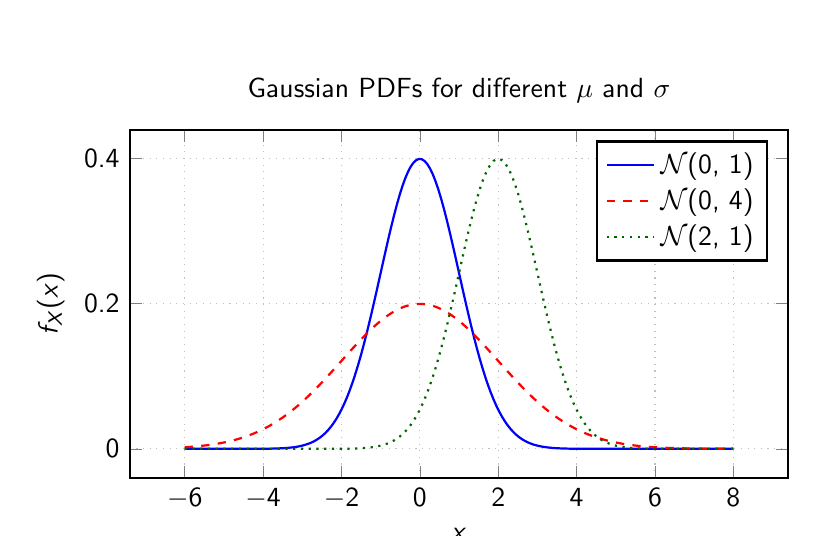
\begin{tikzpicture}
\begin{axis}[
  width=0.82\textwidth, height=6cm,
  xlabel={$x$}, ylabel={$f_X(x)$},
  title={Gaussian PDFs for different $\mu$ and $\sigma$},
  domain=-6:8, samples=200,
  legend pos=north east,
  grid=major, grid style={dotted, gray!50},
  thick
]
  \addplot[blue,  thick]{exp(-(x-0)^2/(2*1^2))/(sqrt(2*pi)*1)};
  \addlegendentry{$\mathcal{N}(0,\,1)$}

  \addplot[red,   thick, dashed]{exp(-(x-0)^2/(2*2^2))/(sqrt(2*pi)*2)};
  \addlegendentry{$\mathcal{N}(0,\,4)$}

  \addplot[black!60!green, thick, dotted]
          {exp(-(x-2)^2/(2*1^2))/(sqrt(2*pi)*1)};
  \addlegendentry{$\mathcal{N}(2,\,1)$}
\end{axis}
\end{tikzpicture}
\caption{Gaussian PDFs.  Increasing $\sigma^2$ widens the bell curve
  (more uncertainty); shifting $\mu$ moves its centre (different
  expected value).}
\label{fig:gauss_pdf}
\end{figure}

\textbf{The 68--95--99.7 rule} (essential for engineering):
\[
  P(\mu - \sigma \leq X \leq \mu + \sigma)    \approx 0.683,\quad
  P(\mu - 2\sigma \leq X \leq \mu + 2\sigma)  \approx 0.954,\quad
  P(\mu - 3\sigma \leq X \leq \mu + 3\sigma)  \approx 0.997.
\]

\begin{examplebox}{Gaussian sensor noise in MATLAB}
A temperature sensor measures a true value of $20\,^\circ$C with
additive Gaussian noise of standard deviation $\sigma = 0.5\,^\circ$C.
Simulate 10\,000 measurements and verify the 68--95--99.7 rule.

\begin{lstlisting}[language=Matlab]
mu    = 20;
sigma = 0.5;
N     = 10000;
rng(42);               % fix random seed for reproducibility

meas  = mu + sigma * randn(1, N);

% Verify 68-95-99.7 rule
in1sig = mean(abs(meas - mu) <= 1*sigma)   % ~0.683
in2sig = mean(abs(meas - mu) <= 2*sigma)   % ~0.954
in3sig = mean(abs(meas - mu) <= 3*sigma)   % ~0.997

% Plot histogram vs true PDF
figure;
histogram(meas, 60, 'Normalization', 'pdf', ...
          'FaceColor', [0.6 0.8 1], 'EdgeColor', 'none');
hold on;
x_range = linspace(17, 23, 300);
pdf_true = normpdf(x_range, mu, sigma);
plot(x_range, pdf_true, 'r-', 'LineWidth', 2);
xlabel('Measurement (deg C)');
ylabel('Probability density');
title('Simulated Gaussian sensor noise');
legend('Histogram','True PDF'); grid on;
\end{lstlisting}

\solution
Running the code confirms all three percentages to within 1\% of
their theoretical values.  \texttt{normpdf(x,mu,sigma)} evaluates the
Gaussian PDF; \texttt{normcdf} evaluates the CDF.

\end{examplebox}

\begin{figure}[htbp]
\centering
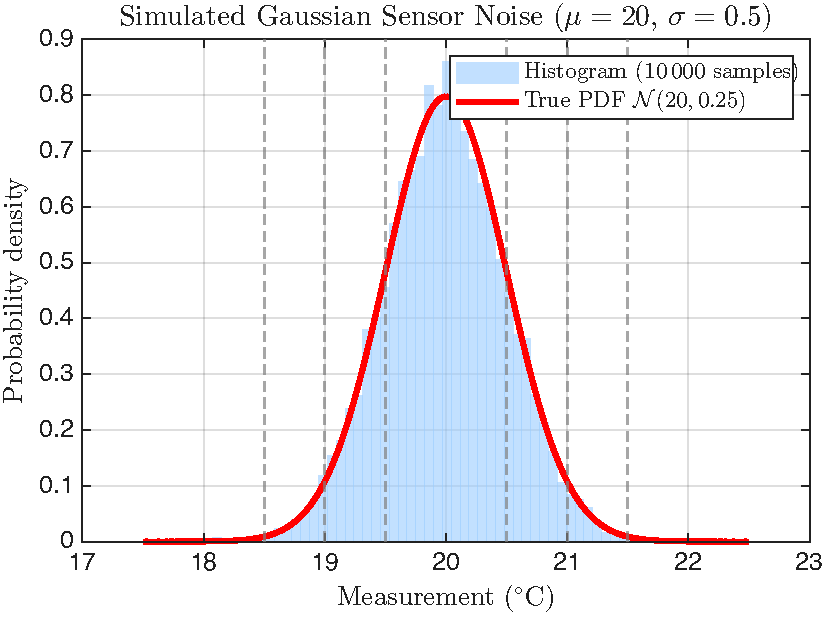
\includegraphics[width=0.72\textwidth]{Figures/fig_app_gauss_hist.pdf}
\caption{Histogram of 10\,000 simulated sensor measurements overlaid with the true Gaussian PDF $\mathcal{N}(20,\,0.25)$.  Dashed lines mark $\pm 1\sigma$, $\pm 2\sigma$, and $\pm 3\sigma$ bounds.}
\label{fig:app_gauss_hist}
\end{figure}

\subsection{Exponential and Other Useful Distributions}

\begin{center}
\renewcommand{\arraystretch}{1.3}
\begin{tabular}{>{\bfseries\sffamily\small}l >{\small}l >{\small}l >{\small}l}
\toprule
Distribution & PDF / PMF & Mean & Variance \\
\midrule
Uniform $\mathcal{U}(a,b)$ &
  $\tfrac{1}{b-a}$ &
  $\tfrac{a+b}{2}$ &
  $\tfrac{(b-a)^2}{12}$ \\
Gaussian $\mathcal{N}(\mu,\sigma^2)$ &
  $\tfrac{1}{\sqrt{2\pi\sigma^2}}e^{-(x-\mu)^2/2\sigma^2}$ &
  $\mu$ & $\sigma^2$ \\
Exponential $\mathrm{Exp}(\lambda)$ &
  $\lambda e^{-\lambda x}$, $x\geq0$ &
  $1/\lambda$ & $1/\lambda^2$ \\
Bernoulli $\mathrm{Bern}(p)$ &
  $p^x(1-p)^{1-x}$, $x\in\{0,1\}$ &
  $p$ & $p(1-p)$ \\
Poisson $\mathrm{Poi}(\lambda)$ &
  $e^{-\lambda}\lambda^k/k!$, $k=0,1,\ldots$ &
  $\lambda$ & $\lambda$ \\
\bottomrule
\end{tabular}
\end{center}

% =============================================================
\section{Expectation, Variance, and Standard Deviation}
\label{sec:app_moments}
% =============================================================

\begin{defnbox}{Expected Value (Mean)}
The \textbf{expected value} (or \textbf{mean}) of a random variable
$X$ is its probability-weighted average:
\[
  \mu = \mathbb{E}[X] =
  \begin{cases}
    \displaystyle\sum_x x\,p_X(x) & \text{(discrete)}, \\[6pt]
    \displaystyle\int_{-\infty}^{\infty} x\,f_X(x)\,\mathrm{d}x &
    \text{(continuous)}.
  \end{cases}
\]
\end{defnbox}

\begin{defnbox}{Variance and Standard Deviation}
The \textbf{variance} measures the average squared deviation from the
mean:
\[
  \sigma^2 = \mathrm{Var}(X) = \mathbb{E}\!\left[(X-\mu)^2\right]
           = \mathbb{E}[X^2] - \mu^2.
\]
The \textbf{standard deviation} $\sigma = \sqrt{\mathrm{Var}(X)}$ has
the same units as $X$ and is the most intuitive measure of spread.
\end{defnbox}

\textbf{Linearity of expectation} (always true, regardless of
dependence):
\[
  \mathbb{E}[aX + bY + c] = a\,\mathbb{E}[X] + b\,\mathbb{E}[Y] + c.
\]

\textbf{Variance under linear transformation:}
\[
  \mathrm{Var}(aX + b) = a^2\,\mathrm{Var}(X).
\]

\begin{examplebox}{Mean and variance of measurement noise}
The measurement noise in a Kalman filter is modelled as
$v_k \sim \mathcal{N}(0, R)$ with $R = 0.25$.  What fraction of
measurements lie within $\pm 1\,^\circ$C of the true value?

\solution
$\sigma = \sqrt{0.25} = 0.5$.  We need
$P(-1 \leq v_k \leq 1) = P(-2\sigma \leq v_k \leq 2\sigma) \approx
0.954$.

\begin{lstlisting}[language=Matlab]
R     = 0.25;
sigma = sqrt(R);        % 0.5

% Probability within +/- 1 degree
prob = normcdf(1, 0, sigma) - normcdf(-1, 0, sigma)  % 0.9545

% Alternatively, using the standard normal
z = 1 / sigma;          % 2 standard deviations
prob2 = 2*normcdf(z) - 1                             % 0.9545

% Mean and variance via Monte Carlo
v = sigma * randn(1, 1e6);
fprintf('Sample mean:     %.4f\n', mean(v))    % ~0
fprintf('Sample variance: %.4f\n', var(v))     % ~0.25
\end{lstlisting}
\end{examplebox}

% =============================================================
\section{Covariance and Correlation}
\label{sec:app_covariance}
% =============================================================

\begin{defnbox}{Covariance}
The \textbf{covariance} of two random variables $X$ and $Y$ measures
how they vary together:
\[
  \mathrm{Cov}(X,Y) = \mathbb{E}\!\left[(X - \mathbb{E}[X])
                       (Y - \mathbb{E}[Y])\right]
                     = \mathbb{E}[XY] - \mathbb{E}[X]\,\mathbb{E}[Y].
\]
Note that $\mathrm{Cov}(X,X) = \mathrm{Var}(X)$.  If $X$ and $Y$ are
independent, $\mathrm{Cov}(X,Y) = 0$ (but the converse is not
generally true).
\end{defnbox}

\begin{defnbox}{Pearson Correlation Coefficient}
The \textbf{correlation coefficient} normalises covariance to the
range $[-1,1]$:
\[
  \rho_{XY} = \frac{\mathrm{Cov}(X,Y)}{\sigma_X \sigma_Y}.
\]
$\rho = 1$: perfect positive linear relationship; $\rho = -1$:
perfect negative; $\rho = 0$: uncorrelated (no linear relationship).
\end{defnbox}

\begin{examplebox}{Covariance and correlation in MATLAB}
\begin{lstlisting}[language=Matlab]
rng(0);
N  = 1000;
x  = randn(N,1);
y1 = 2*x + 0.5*randn(N,1);   % highly correlated with x
y2 = randn(N,1);               % independent of x

% Covariance matrices
C1 = cov(x, y1)    % large off-diagonal entries
C2 = cov(x, y2)    % near-zero off-diagonal

% Correlation coefficients
rho1 = corr(x, y1)   % close to +1
rho2 = corr(x, y2)   % close to  0

% Scatter plots
figure;
subplot(1,2,1); scatter(x, y1, 5, '.'); grid on;
xlabel('x'); ylabel('y_1'); title(sprintf('\\rho = %.2f', rho1));
subplot(1,2,2); scatter(x, y2, 5, 'r.'); grid on;
xlabel('x'); ylabel('y_2'); title(sprintf('\\rho = %.2f', rho2));
\end{lstlisting}

\end{examplebox}

\begin{figure}[htbp]
\centering
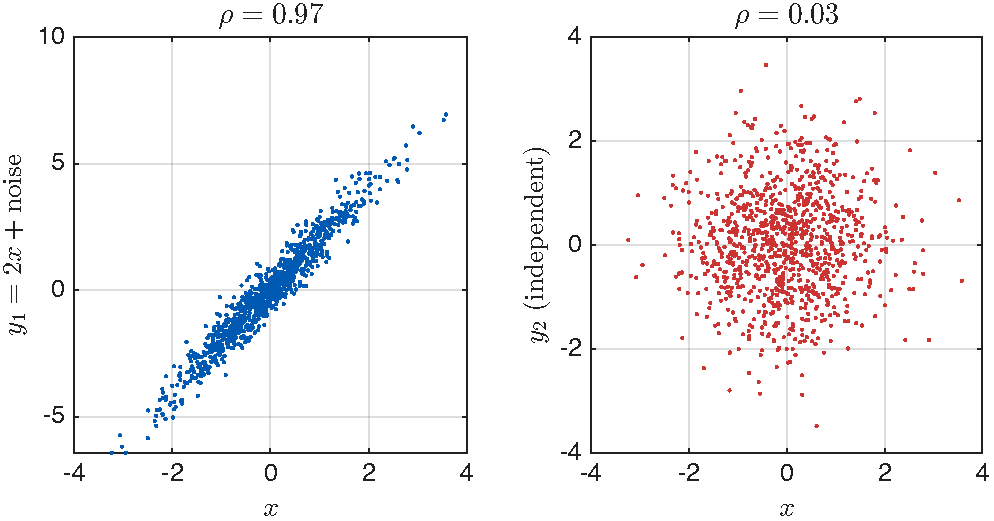
\includegraphics[width=0.85\textwidth]{Figures/fig_app_covariance_scatter.pdf}
\caption{Scatter plots illustrating correlation.  Left: $y_1 = 2x + \text{noise}$ shows strong positive correlation ($\rho \approx 0.97$).  Right: $y_2$ is independent of $x$ ($\rho \approx 0$).}
\label{fig:app_covariance_scatter}
\end{figure}

% =============================================================
\section{The Multivariate Gaussian Distribution}
\label{sec:app_mvgauss}
% =============================================================

State vectors in control systems are multi-dimensional.  The Kalman
filter propagates a full \emph{joint} probability distribution over all
state components simultaneously, which requires the multivariate
generalisation of the Gaussian.

\begin{defnbox}{Multivariate Gaussian $\mathcal{N}(\boldsymbol{\mu}, \Sigma)$}
A random vector $x \in \mathbb{R}^n$ follows a
\textbf{multivariate Gaussian} distribution with mean vector
$\boldsymbol{\mu} \in \mathbb{R}^n$ and
\textbf{covariance matrix} $\Sigma \in \mathbb{R}^{n\times n}$ if its
PDF is:
\[
  f(x) = \frac{1}{(2\pi)^{n/2}\sqrt{\det(\Sigma)}}
                  \exp\!\left(-\frac{1}{2}
                  (x-\boldsymbol{\mu})^\top
                  \Sigma^{-1}
                  (x-\boldsymbol{\mu})\right).
\]
The covariance matrix $\Sigma$ must be \textbf{symmetric positive
semi-definite}: $\Sigma = \Sigma^\top$ and $\Sigma \succeq 0$.
\end{defnbox}

The diagonal entries of $\Sigma$ are the individual variances:
$\Sigma_{ii} = \mathrm{Var}(x_i)$.  The off-diagonal entries are
covariances: $\Sigma_{ij} = \mathrm{Cov}(x_i, x_j)$.

\begin{figure}[htbp]
\centering
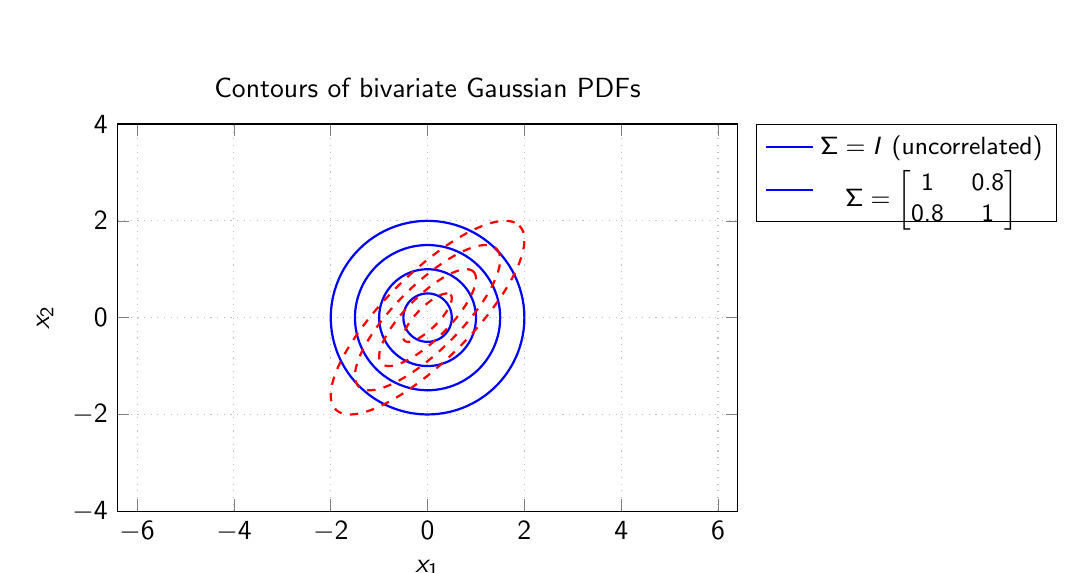
\begin{tikzpicture}
\begin{axis}[
  width=0.78\textwidth, height=6.5cm,
  title={Contours of bivariate Gaussian PDFs},
  xlabel={$x_1$}, ylabel={$x_2$},
  xmin=-4, xmax=4, ymin=-4, ymax=4,
  axis equal,
  grid=major, grid style={dotted, gray!50},
  legend pos=outer north east,
  legend style={font=\small}
]
  % Uncorrelated: contours are circles
  \foreach \r in {0.5, 1.0, 1.5, 2.0}{
    \addplot[blue, thick, domain=0:360, samples=100]
        ({\r*cos(x)}, {\r*sin(x)});
  }
  \addlegendentry{$\Sigma=I$ (uncorrelated)}

  % Correlated: contours are tilted ellipses
  % Sigma = [1 0.8; 0.8 1], eigendecomp gives tilt
  \foreach \r in {0.5, 1.0, 1.5, 2.0}{
    \addplot[red, dashed, thick, domain=0:360, samples=120]
        ({0.949*\r*cos(x) + 0.316*\r*sin(x)},
         {0.949*\r*cos(x) - 0.316*\r*sin(x)});
  }
  \addlegendentry{$\Sigma=\begin{bmatrix}1&0.8\\0.8&1\end{bmatrix}$}
\end{axis}
\end{tikzpicture}
\caption{Equal-probability contours of two bivariate Gaussian
  distributions.  When $\Sigma = I$ the contours are circles
  (independent components).  When off-diagonal covariance is large the
  contours tilt into ellipses aligned with the correlated direction.}
\label{fig:bivariate_gauss}
\end{figure}

\begin{notebox}{Covariance matrices in the Kalman filter}
  The Kalman filter maintains the state estimate as
  $x_k \sim \mathcal{N}(\hat{x}_k, P_k)$,
  where $P_k$ is the \textbf{error covariance matrix}.  At each step:
  \begin{itemize}[noitemsep]
    \item \textbf{Prediction}: $P$ grows (uncertainty increases
          because the model is imperfect).
    \item \textbf{Correction}: $P$ shrinks (the measurement reduces
          uncertainty).
  \end{itemize}
  The Kalman gain $K$ is precisely the factor that balances how much
  to trust the model prediction versus the new measurement.
\end{notebox}

\begin{examplebox}{Multivariate Gaussian samples in MATLAB}
Generate samples from a bivariate Gaussian with
$\boldsymbol{\mu} = [1,\;-2]^\top$ and
$\Sigma = \begin{bmatrix} 2 & 0.8 \\ 0.8 & 1 \end{bmatrix}$.

\begin{lstlisting}[language=Matlab]
mu    = [1; -2];
Sigma = [2, 0.8; 0.8, 1];

% Check Sigma is positive definite
eig(Sigma)           % both positive: [0.4781; 2.5219]

% Draw 2000 samples
rng(1);
N       = 2000;
samples = mvnrnd(mu', Sigma, N);  % N x 2 matrix

% Plot
figure;
scatter(samples(:,1), samples(:,2), 8, '.', ...
        'MarkerEdgeColor', [0.2 0.4 0.8]);
hold on;
plot(mu(1), mu(2), 'r+', 'MarkerSize', 15, 'LineWidth', 2);
xlabel('x_1'); ylabel('x_2');
title('Samples from \mathcal{N}(\mu, \Sigma)');
legend('Samples','Mean'); grid on; axis equal;

% Verify sample statistics
fprintf('Sample mean:  [%.3f, %.3f]\n', mean(samples));
disp('Sample covariance:'); disp(cov(samples))
\end{lstlisting}

\end{examplebox}

\begin{figure}[htbp]
\centering
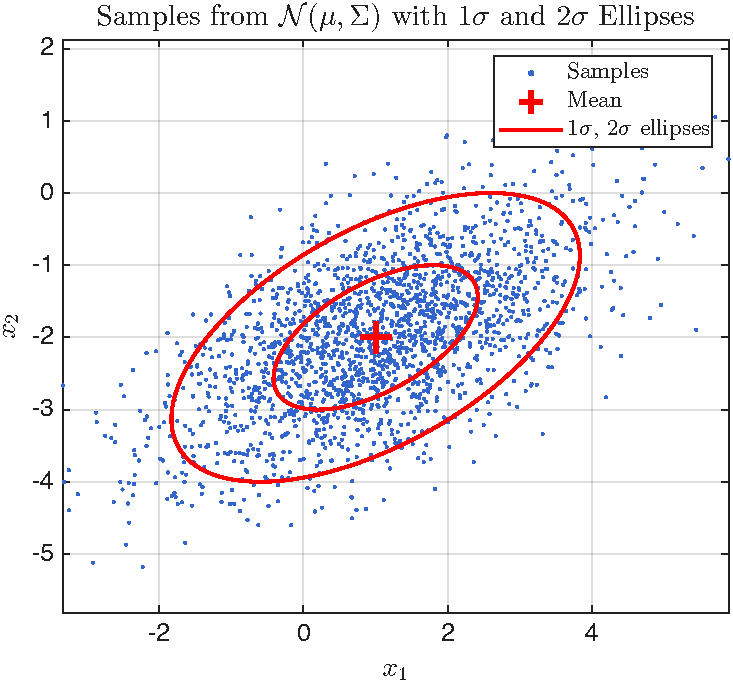
\includegraphics[width=0.65\textwidth]{Figures/fig_app_mvnrnd_samples.pdf}
\caption{2\,000 samples from a bivariate Gaussian with $\boldsymbol{\mu} = [1,\,-2]^\top$ and correlated covariance.  Red ellipses show the $1\sigma$ and $2\sigma$ contours, which are tilted due to the positive off-diagonal covariance.}
\label{fig:app_mvnrnd_samples}
\end{figure}

% =============================================================
\section{Conditional Multivariate Gaussian}
\label{sec:app_cond_gauss}
% =============================================================

A second closure property of Gaussians---equally important as linear transformations---is that \emph{conditioning} a joint Gaussian on some of its components produces another Gaussian. This is the mathematical foundation of both the Kalman filter update step and Gaussian process regression (Chapter~11).

\begin{defnbox}{Conditional Gaussian Distribution}
Suppose $\begin{bmatrix} x_a \\ x_b \end{bmatrix} \sim \mathcal{N}\!\left(\begin{bmatrix} \mu_a \\ \mu_b \end{bmatrix},\; \begin{bmatrix} \Sigma_{aa} & \Sigma_{ab} \\ \Sigma_{ba} & \Sigma_{bb} \end{bmatrix}\right)$.
Then the conditional distribution of $x_a$ given $x_b = \bar{x}_b$ is:
\[
	x_a \mid x_b = \bar{x}_b \;\sim\; \mathcal{N}\!\bigl(\mu_{a|b},\; \Sigma_{a|b}\bigr)
\]
where:
\begin{align*}
	\mu_{a|b} &= \mu_a + \Sigma_{ab}\,\Sigma_{bb}^{-1}\,(\bar{x}_b - \mu_b) \\
	\Sigma_{a|b} &= \Sigma_{aa} - \Sigma_{ab}\,\Sigma_{bb}^{-1}\,\Sigma_{ba}
\end{align*}
\end{defnbox}

Two observations are worth noting:
\begin{itemize}[noitemsep]
	\item The conditional mean $\mu_{a|b}$ is the prior mean $\mu_a$ plus a correction proportional to how far the observed value $\bar{x}_b$ deviates from its prior mean $\mu_b$. The matrix $\Sigma_{ab}\,\Sigma_{bb}^{-1}$ determines how much $x_a$ adjusts in response --- this is exactly the structure of the Kalman gain.
	\item The conditional covariance $\Sigma_{a|b}$ does not depend on the observed value $\bar{x}_b$; it depends only on the prior covariance structure. Observing $x_b$ always reduces variance by the same amount, regardless of what value is observed.
\end{itemize}

\begin{examplebox}{Conditional Gaussian: numerical example}
Let $\begin{bmatrix} x_1 \\ x_2 \end{bmatrix} \sim \mathcal{N}\!\left(\begin{bmatrix} 0 \\ 0 \end{bmatrix},\; \begin{bmatrix} 1 & 0.8 \\ 0.8 & 1 \end{bmatrix}\right)$. Compute $x_1 \mid x_2 = 1.5$.

\solution
Identify $\mu_a = 0$, $\mu_b = 0$, $\Sigma_{aa} = 1$, $\Sigma_{ab} = 0.8$, $\Sigma_{bb} = 1$. Then:
\begin{align*}
	\mu_{1|2} &= 0 + 0.8 \cdot 1^{-1} \cdot (1.5 - 0) = 1.2 \\
	\sigma^2_{1|2} &= 1 - 0.8 \cdot 1^{-1} \cdot 0.8 = 0.36
\end{align*}
So $x_1 \mid x_2 = 1.5 \;\sim\; \mathcal{N}(1.2,\; 0.36)$. Knowing $x_2 = 1.5$ shifts our prediction of $x_1$ from~0 to~1.2, and reduces the variance from~1 to~0.36.

This is exactly how Gaussian process prediction works (Chapter~11, Section~11.2.1): the ``training outputs'' play the role of $x_b$, and the ``test output'' plays the role of $x_a$. The kernel matrix provides the covariance structure.
\end{examplebox}

% =============================================================
\section{Chance Constraints and the Inverse CDF}
\label{sec:app_chance_constraints}
% =============================================================

In stochastic MPC and GP-MPC (Chapter~11), hard state constraints $x_k \le x_{\max}$ cannot be guaranteed when the state is uncertain. Instead, we require the constraint to hold with high probability:
\[
	\Pr(x_k \le x_{\max}) \ge 1 - \delta
\]
where $\delta \in (0, 1)$ is a small violation probability (e.g.\ $\delta = 0.05$ for 95\% confidence).

If $x_k \sim \mathcal{N}(\mu_k, \sigma_k^2)$, this chance constraint can be converted to a \emph{deterministic} constraint on the mean:
\[
	\mu_k + \Phi^{-1}(1-\delta)\,\sigma_k \le x_{\max}
\]
where $\Phi^{-1}$ is the inverse CDF (quantile function) of the standard normal distribution. Common values: $\Phi^{-1}(0.95) \approx 1.645$, $\Phi^{-1}(0.975) \approx 1.960$, $\Phi^{-1}(0.99) \approx 2.326$.

The term $\Phi^{-1}(1-\delta)\,\sigma_k$ is the \emph{constraint tightening}: the safety margin grows with uncertainty $\sigma_k$ and with the required confidence level $1-\delta$. In MATLAB: \texttt{kappa = norminv(1 - delta)}.

% =============================================================
\section{Linear Transformations of Gaussian Variables}
\label{sec:app_linear_gauss}
% =============================================================

A crucial property that makes Gaussian distributions so convenient for
control is that they are \emph{closed under linear transformations}: a
linear function of a Gaussian is still Gaussian.

\begin{defnbox}{Linear Transformation of a Gaussian Vector}
If $x \sim \mathcal{N}(\boldsymbol{\mu}, \Sigma)$ and
$y = Ax + b$, then:
\[
  y \sim \mathcal{N}\!\left(
    A\boldsymbol{\mu} + b,\;
    A\Sigma A^\top
  \right).
\]
\end{defnbox}

This is exactly the \textbf{predict step} of the Kalman filter.  If
the state $x_k \sim \mathcal{N}(\hat{x}_k, P_k)$
and the system evolves as $x_{k+1} = Ax_k +
w_k$ with process noise
$w_k \sim \mathcal{N}(0, Q)$, then the predicted
state distribution is:
\[
  x_{k+1} \sim \mathcal{N}\!\left(
    A\hat{x}_k,\;
    A P_k A^\top + Q
  \right).
\]
No approximation is involved — the result is exact because all
operations are linear and all distributions are Gaussian.

\begin{examplebox}{Propagating uncertainty through a linear system}
A one-dimensional system has $x_{k+1} = 0.9\,x_k + w_k$ with
$w_k \sim \mathcal{N}(0, 0.01)$.  The initial state is
$x_0 \sim \mathcal{N}(5, 1)$.  Propagate the mean and variance for
10 steps.

\solution
At each step: $\mu_{k+1} = 0.9\,\mu_k$ and
$\sigma^2_{k+1} = 0.81\,\sigma^2_k + 0.01$.  The variance decays
towards the steady-state value
$\sigma^2_\infty = 0.01/(1-0.81) \approx 0.053$.

\begin{lstlisting}[language=Matlab]
a     = 0.9;
Q     = 0.01;    % process noise variance
mu    = 5;
P     = 1;       % initial variance
N     = 10;

mu_log = zeros(1,N+1);  P_log = zeros(1,N+1);
mu_log(1) = mu;          P_log(1) = P;

for k = 1:N
    mu = a * mu;
    P  = a^2 * P + Q;
    mu_log(k+1) = mu;
    P_log(k+1)  = P;
end

figure;
subplot(2,1,1);
plot(0:N, mu_log, 'b-o', 'LineWidth', 1.5);
ylabel('\mu_k'); title('Propagated mean'); grid on;

subplot(2,1,2);
plot(0:N, P_log, 'r-o', 'LineWidth', 1.5);
yline(Q/(1-a^2), 'k--', 'Steady state', 'LineWidth', 1);
ylabel('\sigma^2_k'); xlabel('Step k');
title('Propagated variance'); grid on;
\end{lstlisting}

\end{examplebox}

\begin{figure}[htbp]
\centering
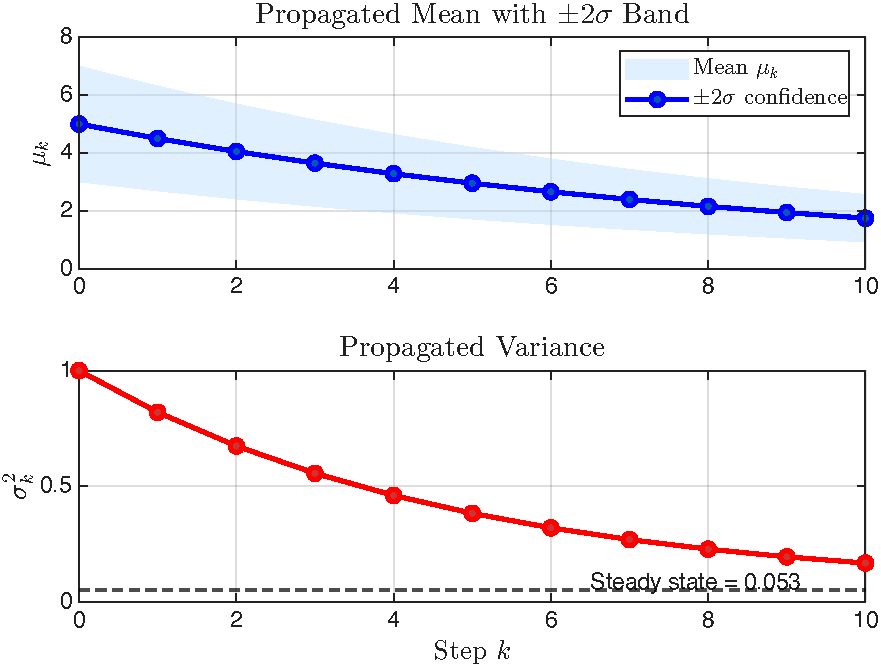
\includegraphics[width=0.75\textwidth]{Figures/fig_app_uncertainty_prop.pdf}
\caption{Propagation of a Gaussian state distribution through $x_{k+1} = 0.9\,x_k + w_k$.  Top: the mean decays towards zero with a $\pm 2\sigma$ confidence band.  Bottom: the variance converges to the steady-state value $\sigma^2_\infty = Q/(1 - a^2) \approx 0.053$.}
\label{fig:app_uncertainty_prop}
\end{figure}

% =============================================================
\section{Stochastic Processes}
\label{sec:app_stochastic}
% =============================================================

A \textbf{stochastic process} is a sequence of random variables
indexed by time: $\{X_k\}_{k=0}^{\infty}$ (discrete time) or
$\{X(t)\}_{t\geq0}$ (continuous time).  In control, the key
stochastic processes are:

\begin{itemize}[noitemsep]
  \item \textbf{White noise}: uncorrelated sequence where each sample
        is drawn independently from the same distribution.  Used to
        model process noise $w_k$ and measurement noise $v_k$ in state-space models.
  \item \textbf{Random walk}: $X_{k+1} = X_k + w_k$ where $w_k$ is
        white noise.  The variance grows without bound.
  \item \textbf{Markov process}: the future depends only on the
        present state, not the past.  State-space models are
        (first-order) Markov by construction: $x_{k+1} = f(x_k, u_k, w_k)$.
\end{itemize}

\begin{defnbox}{White Noise Assumptions in State-Space Control}
The standard Kalman filter assumptions are:
\begin{align*}
  w_k &\sim \mathcal{N}(0, Q), \quad
  \text{(process noise)} \\
  v_k &\sim \mathcal{N}(0, R), \quad
  \text{(measurement noise)} \\
  \mathbb{E}[w_k w_j^\top] &= Q\,\delta_{kj}, \quad
  \text{(uncorrelated across time)} \\
  \mathbb{E}[v_k v_j^\top] &= R\,\delta_{kj}, \quad
  \mathbb{E}[w_k v_j^\top] &= 0,
\end{align*}
where $\delta_{kj} = 1$ if $k=j$, else $0$ (Kronecker delta).
Matrices $Q \succeq 0$ and $R \succ 0$ are the noise covariance
matrices that appear explicitly in the Kalman filter equations.
\end{defnbox}

\begin{examplebox}{Simulating white noise and a random walk}
\begin{lstlisting}[language=Matlab]
N     = 200;
Q     = 0.5;      % process noise variance
rng(7);
w     = sqrt(Q) * randn(1, N);   % white noise sequence

% Verify whiteness: autocorrelation should be near zero for lag > 0
figure;
subplot(3,1,1);
plot(w); xlabel('k'); ylabel('w_k');
title('White noise sequence'); grid on;

subplot(3,1,2);
maxlag = 20;
acf = zeros(1, maxlag+1);
w_c = w - mean(w);
c0 = sum(w_c.^2);
for lag = 0:maxlag
    acf(lag+1) = sum(w_c(1:end-lag).*w_c(lag+1:end))/c0;
end
stem(0:maxlag, acf, 'filled', 'LineWidth', 1.5);
xlabel('Lag'); ylabel('ACF');
title('Autocorrelation of white noise');
yline(1.96/sqrt(N), 'r--'); yline(-1.96/sqrt(N), 'r--');

% Random walk: x_{k+1} = x_k + w_k
x = cumsum(w);
subplot(3,1,3);
plot(x, 'r'); xlabel('k'); ylabel('x_k');
title('Random walk (cumulative sum of white noise)'); grid on;
\end{lstlisting}
\solution
The autocorrelation plot confirms that white noise has zero
correlation at all non-zero lags (within statistical fluctuation).
The random walk drifts unpredictably because its variance grows as
$k \cdot Q$.

\end{examplebox}

\begin{figure}[htbp]
\centering
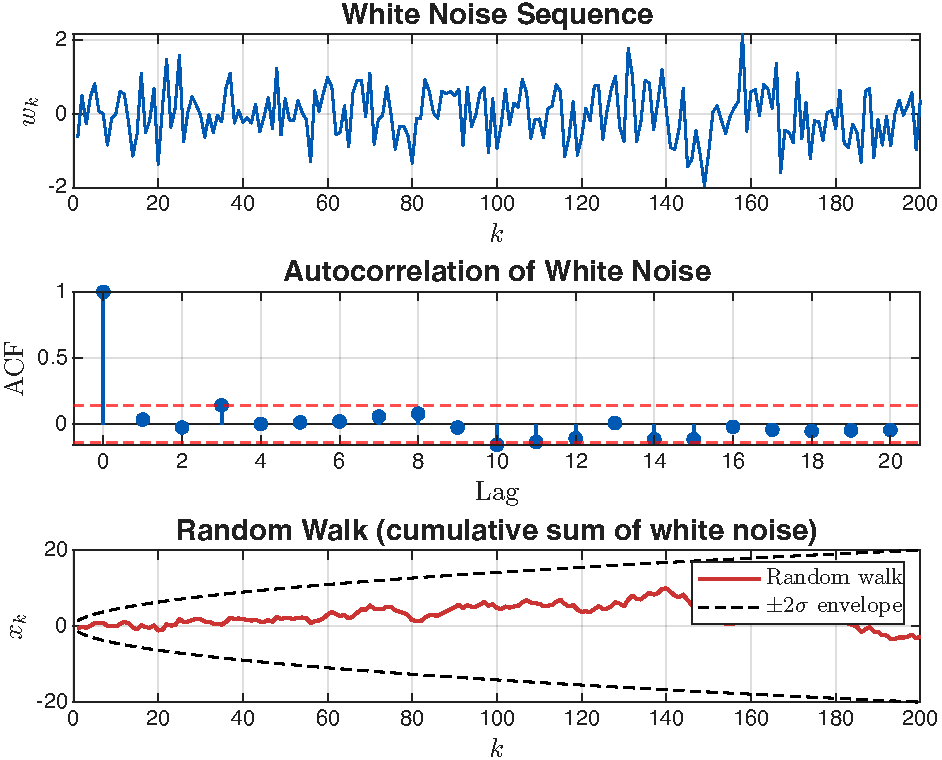
\includegraphics[width=0.82\textwidth]{Figures/fig_app_white_noise_rw.pdf}
\caption{Top: a white noise sequence $w_k \sim \mathcal{N}(0, 0.5)$.  Middle: its autocorrelation function, confirming zero correlation at all non-zero lags.  Bottom: the random walk $x_k = \sum_{i=1}^{k} w_i$ with the $\pm 2\sigma$ envelope $\pm 2\sqrt{kQ}$ showing unbounded variance growth.}
\label{fig:app_white_noise_rw}
\end{figure}

% =============================================================
\section{The Law of Large Numbers and the Central Limit Theorem}
\label{sec:app_lln_clt}
% =============================================================

These two theorems are the bedrock of statistical intuition.

\begin{defnbox}{Law of Large Numbers (LLN)}
Let $X_1, X_2, \ldots, X_N$ be independent, identically distributed
(i.i.d.) random variables with mean $\mu$.  The sample mean converges
to the true mean as the sample size grows:
\[
  \bar{X}_N = \frac{1}{N}\sum_{i=1}^N X_i \;\xrightarrow{\;N\to\infty\;}\; \mu.
\]
\end{defnbox}

\begin{defnbox}{Central Limit Theorem (CLT)}
Under the same conditions (i.i.d., finite variance $\sigma^2$), the
\emph{standardised} sample mean converges in distribution to a
standard Gaussian:
\[
  \frac{\bar{X}_N - \mu}{\sigma/\sqrt{N}}
  \;\xrightarrow{\;d\;}\;
  \mathcal{N}(0,1)
  \quad \text{as } N \to \infty.
\]
This is why Gaussian noise is such a universal model: it emerges
naturally as the aggregate effect of many small, independent
perturbations.
\end{defnbox}

\begin{examplebox}{Demonstrating the CLT in MATLAB}
Show that the sample mean of $N$ uniform random variables approaches
a Gaussian as $N$ increases.

\begin{lstlisting}[language=Matlab]
n_trials = 5000;
figure;

for idx = 1:4
    N = 10^idx;                          % N = 10, 100, 1000, 10000
    % Sum N uniform[0,1] samples, then standardise
    raw  = rand(n_trials, N);
    xbar = mean(raw, 2);                 % n_trials x 1 sample means
    mu_u = 0.5;  sig_u = 1/sqrt(12*N);  % theoretical mean and std
    z    = (xbar - mu_u) / sig_u;

    subplot(2,2,idx);
    histogram(z, 40, 'Normalization','pdf', ...
              'FaceColor',[0.6 0.8 1], 'EdgeColor','none');
    hold on;
    x_range = linspace(-4, 4, 200);
    plot(x_range, normpdf(x_range), 'r-', 'LineWidth', 2);
    title(sprintf('N = %d', N));
    xlabel('z'); ylabel('PDF'); grid on;
    xlim([-4 4]);
end
sgtitle('Central Limit Theorem: convergence to Gaussian');
\end{lstlisting}
\solution
Even for $N=10$ the histogram already resembles a bell curve.  By
$N=1000$ the agreement with the standard Gaussian (red curve) is
almost perfect.

\end{examplebox}

\begin{figure}[htbp]
\centering
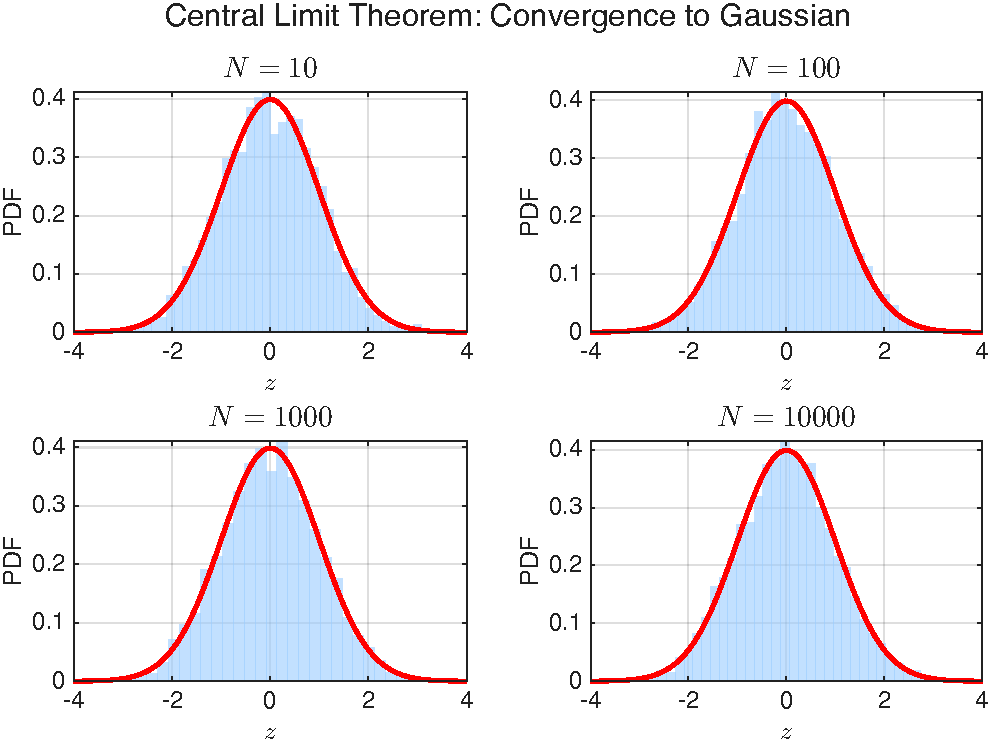
\includegraphics[width=0.82\textwidth]{Figures/fig_app_clt_demo.pdf}
\caption{Central Limit Theorem in action.  The standardised sample mean of $N$ uniform random variables (blue histogram) converges to the standard Gaussian (red curve) as $N$ increases.}
\label{fig:app_clt_demo}
\end{figure}

% =============================================================
\section{Monte Carlo Methods}
\label{sec:app_montecarlo}
% =============================================================

Monte Carlo methods approximate expectations and probabilities by
drawing many random samples.  They are used in stochastic MPC to
evaluate chance constraints (e.g.\ ``what fraction of scenarios
violate a temperature bound?'') and in RL to estimate policy value
functions.

\begin{defnbox}{Monte Carlo Estimation}
To estimate $\mathbb{E}[g(X)]$ for some function $g$ and random
variable $X$:
\begin{enumerate}[noitemsep]
  \item Draw $N$ i.i.d.\ samples $x^{(1)}, x^{(2)}, \ldots, x^{(N)}$
        from the distribution of $X$.
  \item Compute the sample average:
        $\hat{\mathbb{E}}[g(X)] = \dfrac{1}{N}\sum_{i=1}^N g(x^{(i)})$.
\end{enumerate}
By the LLN this estimate converges to the true expectation.  The
standard error of the estimate is $\sigma_{g(X)}/\sqrt{N}$, so
accuracy improves as $1/\sqrt{N}$.
\end{defnbox}

\begin{examplebox}{Monte Carlo chance constraint evaluation}
In a stochastic MPC application, room temperature at the next step is
$x_1 \sim \mathcal{N}(21.5,\; 0.04)$ (mean 21.5$^\circ$C, variance
0.04).  Estimate the probability that the comfort constraint
$x_1 \geq 21\,^\circ$C is satisfied.

\begin{lstlisting}[language=Matlab]
mu_x  = 21.5;
var_x = 0.04;
N     = 100000;
rng(3);
x_samples = mu_x + sqrt(var_x) * randn(1, N);

% Monte Carlo probability estimate
p_mc      = mean(x_samples >= 21)     % ~0.9938

% Exact answer via CDF
p_exact   = 1 - normcdf(21, mu_x, sqrt(var_x))  % 0.9938

fprintf('Monte Carlo: %.4f\n', p_mc);
fprintf('Exact:       %.4f\n', p_exact);
\end{lstlisting}
\solution
Both methods give $P(x_1 \geq 21) \approx 0.9938$, i.e.\ the
comfort constraint is satisfied 99.4\% of the time.  In stochastic
MPC this would be expressed as the chance constraint
$P(x_1 \geq 21) \geq 0.95$.

\end{examplebox}

\begin{figure}[htbp]
\centering
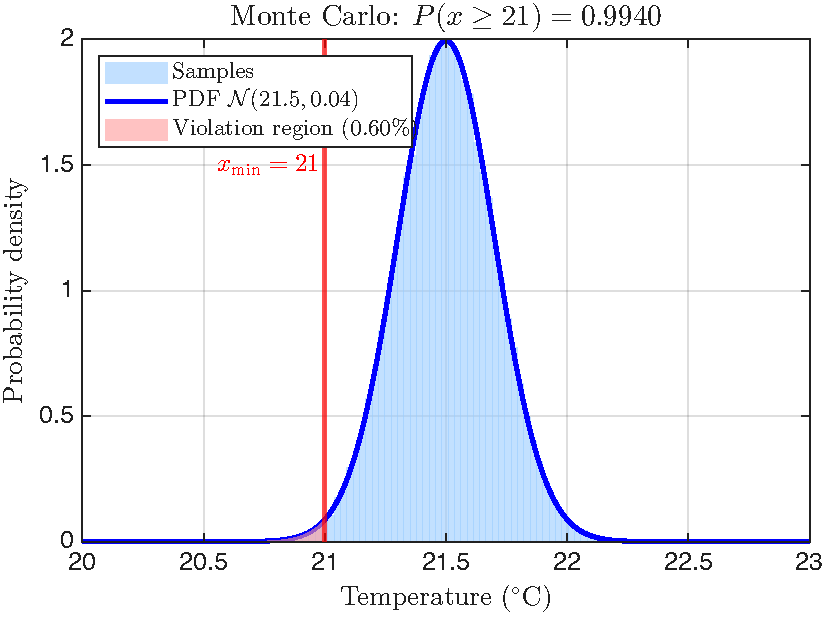
\includegraphics[width=0.72\textwidth]{Figures/fig_app_monte_carlo.pdf}
\caption{Monte Carlo evaluation of the chance constraint $P(x \geq 21) \geq 0.95$.  The shaded red region to the left of $x_{\min} = 21$ is the constraint violation area, which contains only $\approx 0.6\%$ of the probability mass.}
\label{fig:app_monte_carlo}
\end{figure}

% =============================================================
\section{Connecting Probability to the Kalman Filter}
\label{sec:app_kalman_prob}
% =============================================================

With the tools of this appendix, the Kalman filter equations can now
be understood probabilistically rather than just algorithmically.

The \textbf{state-space model} is:
\begin{align}
  {x}_{k+1} &= A{x}_k + B{u}_k + {w}_k,
  \qquad {w}_k \sim \mathcal{N}({0}, Q), \label{eq:ss1}\\
  {y}_k     &= C{x}_k + {v}_k,
  \qquad {v}_k \sim \mathcal{N}({0}, R). \label{eq:ss2}
\end{align}

The Kalman filter maintains a Gaussian belief over the state:
\[
  p({x}_k \mid {y}_{0:k}) = \mathcal{N}(\hat{{x}}_k, P_k).
\]

\textbf{Predict step} (propagate using the system model):
\begin{align}
  \hat{{x}}_{k|k-1} &= A\hat{{x}}_{k-1} + B{u}_{k-1}, \\
  P_{k|k-1}                 &= A P_{k-1} A^\top + Q.
\end{align}
This is the linear transformation rule from
Section~\ref{sec:app_linear_gauss}.

\textbf{Correct step} (update using the new measurement):
\begin{align}
  K_k               &= P_{k|k-1} C^\top
                        (C P_{k|k-1} C^\top + R)^{-1},
                        \quad\text{(Kalman gain)} \\
  \hat{{x}}_k &= \hat{{x}}_{k|k-1}
                        + K_k({y}_k - C\hat{{x}}_{k|k-1}), \\
  P_k               &= (I - K_k C)\,P_{k|k-1}.
\end{align}
The Kalman gain $K_k$ is the optimal Bayesian weighting between the
model prediction and the measurement.  When $R$ is large (noisy
sensor), $K_k \to 0$ and the filter trusts the model.  When $Q$ is
large (uncertain model), $K_k$ increases and the filter trusts the
measurement.

\begin{examplebox}{One-dimensional Kalman filter in MATLAB}
Estimate the position of a slowly drifting signal with process noise
$Q = 0.1$ and measurement noise $R = 2$.

\begin{lstlisting}[language=Matlab]
A = 1;  C = 1;  Q = 0.1;  R = 2;
N = 60;  rng(5);

% Simulate true state and measurements
x_true = cumsum([10, sqrt(Q)*randn(1,N-1)]);
y_meas = x_true + sqrt(R)*randn(1,N);

% Kalman filter
x_hat = zeros(1,N);  P = 10;  x_est = 10;

for k = 1:N
    % Predict
    x_pred = A * x_est;
    P_pred = A^2 * P + Q;

    % Correct
    K      = P_pred * C / (C^2 * P_pred + R);
    x_est  = x_pred + K * (y_meas(k) - C*x_pred);
    P      = (1 - K*C) * P_pred;
    x_hat(k) = x_est;
end

% Plot
figure;
plot(x_true, 'k-',  'LineWidth', 1.5); hold on;
plot(y_meas, 'b.',  'MarkerSize', 8);
plot(x_hat,  'r-',  'LineWidth', 2);
legend('True state','Measurements','Kalman estimate');
xlabel('Time step k'); ylabel('Position');
title('1-D Kalman Filter'); grid on;
\end{lstlisting}
\solution
The Kalman estimate (red) tracks the true state (black) much more
closely than the raw noisy measurements (blue dots), demonstrating the
filter's noise-rejection capability.

\end{examplebox}

\begin{figure}[htbp]
\centering
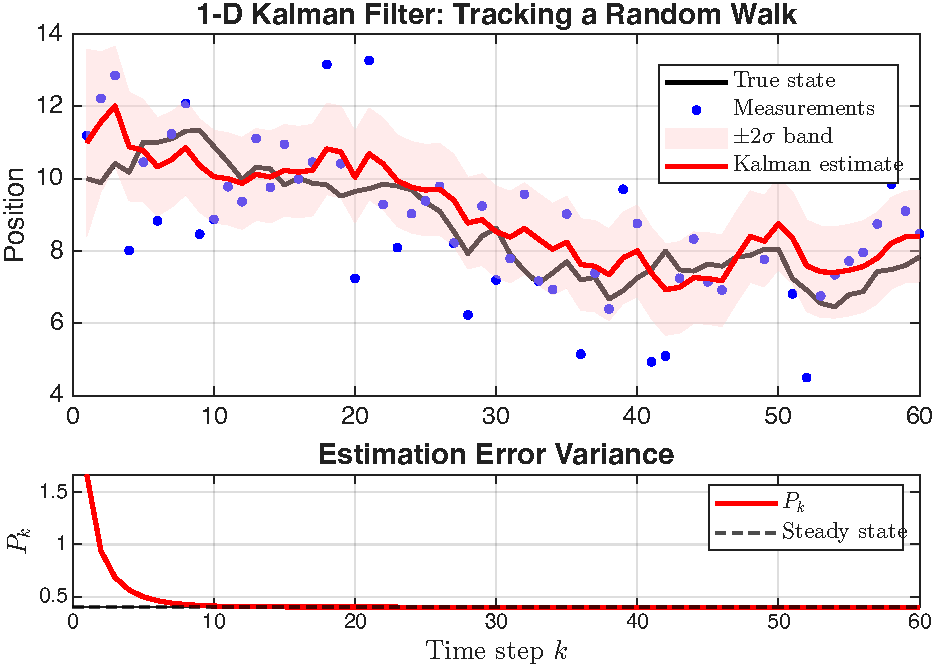
\includegraphics[width=0.82\textwidth]{Figures/fig_app_kalman_1d.pdf}
\caption{1-D Kalman filter tracking a random walk.  Top: the Kalman estimate (red) tracks the true state (black) far more closely than the noisy measurements (blue dots); the shaded band shows $\pm 2\sigma$ confidence.  Bottom: the estimation error variance $P_k$ converges quickly to its steady-state value.}
\label{fig:app_kalman_1d}
\end{figure}

% =============================================================
\section{Probability in Reinforcement Learning}
\label{sec:app_rl_prob}
% =============================================================

Reinforcement Learning frames the control problem as a
\textbf{Markov Decision Process} (MDP), which is a direct application
of the probabilistic tools developed in this appendix.

\begin{defnbox}{Markov Decision Process}
An MDP is defined by the tuple $(\mathcal{S}, \mathcal{A},
\mathcal{P}, r, \gamma)$:
\begin{itemize}[noitemsep]
  \item $\mathcal{S}$: state space (e.g.\ room temperatures)
  \item $\mathcal{A}$: action space (e.g.\ heater power levels)
  \item $\mathcal{P}(s' \mid s, a)$: \textbf{transition probability} —
        probability of reaching state $s'$ from state $s$ under action
        $a$
  \item $r(s,a)$: reward function (e.g.\ negative energy cost)
  \item $\gamma \in [0,1)$: discount factor for future rewards
\end{itemize}
The agent's goal is to find a policy $\pi(a \mid s)$ (a conditional
probability distribution over actions given states) that maximises
the \textbf{expected discounted return}:
\[
  J(\pi) = \mathbb{E}_\pi\!\left[\sum_{k=0}^{\infty} \gamma^k r(s_k, a_k)\right].
\]
\end{defnbox}

Every concept used in this definition — conditional probability,
expectation, Markov property — has been covered in the earlier sections
of this appendix.  The connection between RL and MPC is that both seek
to maximise a sum of future rewards/costs; RL does so by
\emph{learning} the optimal policy from data rather than by solving an
explicit optimisation problem at each step.

% =============================================================
\section{Quick Reference: MATLAB Commands for Probability}
\label{sec:app_prob_ref}
% =============================================================

\begin{center}
\renewcommand{\arraystretch}{1.35}
\begin{tabular}{>{\ttfamily\small}l >{\small}l >{\small}l}
\toprule
\normalfont\textbf{MATLAB command} & \textbf{Operation} &
\textbf{Notes} \\
\midrule
randn(m,n)           & Standard Gaussian samples     & $\mathcal{N}(0,1)$, size $m\times n$ \\
rand(m,n)            & Uniform $[0,1]$ samples       & Size $m\times n$ \\
rng(seed)            & Set random seed               & For reproducibility \\
normpdf(x,mu,sig)    & Gaussian PDF                  & Scalar or vector $x$ \\
normcdf(x,mu,sig)    & Gaussian CDF                  & $P(X\leq x)$ \\
norminv(p,mu,sig)    & Inverse CDF (quantile)        & $x$ such that $P(X\leq x)=p$ \\
mvnrnd(mu,Sigma,N)   & Multivariate Gaussian samples & $N$ rows \\
mvnpdf(X,mu,Sigma)   & Multivariate Gaussian PDF     & \\
mean(x)              & Sample mean                   & Along first non-singleton dim \\
var(x)               & Sample variance               & Unbiased ($N-1$ denominator) \\
std(x)               & Sample standard deviation     & $\sqrt{\texttt{var}(x)}$ \\
cov(X)               & Sample covariance matrix      & \texttt{X} is $N\times p$ data matrix \\
corr(x,y)            & Pearson correlation            & Returns scalar in $[-1,1]$ \\
autocorr(x,n)        & Sample autocorrelation         & Up to lag $n$ \\
histogram(x,k)       & Histogram                     & Use \texttt{'Normalization','pdf'} \\
eig(Sigma)           & Eigenvalues of $\Sigma$        & Check positive definiteness \\
chol(Sigma)          & Cholesky factorisation         & For sampling multivariate Gaussian \\
\bottomrule
\end{tabular}
\end{center}

\begin{summarybox}{Probability Summary for Control Engineers}
\begin{enumerate}[noitemsep]
  \item \textbf{Everything uncertain is a random variable.}  Sensor
        noise, model errors, and disturbances are all modelled as
        random variables with known distributions.
  \item \textbf{The Gaussian is central.}  Sensor noise and process
        disturbances are almost always modelled as Gaussian because of
        the CLT, and because Gaussians are closed under linear
        transformations.
  \item \textbf{Mean and covariance matrix} fully characterise a
        Gaussian distribution.  The Kalman filter propagates exactly
        these two quantities.
  \item \textbf{Bayes' theorem is the theoretical backbone} of all
        state estimation.  The Kalman filter is its exact solution
        under linearity and Gaussianity.
  \item \textbf{$Q$ and $R$ are design choices.}  The process noise
        covariance $Q$ and measurement noise covariance $R$ in the
        Kalman filter determine how much the filter trusts the model
        versus the sensor.  Larger $R$ $\Rightarrow$ trust the model
        more; larger $Q$ $\Rightarrow$ trust the sensor more.
  \item \textbf{Chance constraints in stochastic MPC} replace hard
        bounds with probabilistic ones:
        $P(Cx_k \leq d) \geq 1-\epsilon$.  Monte Carlo or analytical
        Gaussian CDF methods evaluate these constraints.
  \item \textbf{RL uses expectations everywhere.}  Value functions,
        policy gradients, and Bellman equations are all defined in
        terms of expected rewards under a probability distribution over
        future trajectories.
\end{enumerate}
\end{summarybox}


	\end{appendices}

	\backmatter
	\bibliographystyle{plainnat}
	\bibliography{references}
\end{document}